% Options for packages loaded elsewhere
\PassOptionsToPackage{unicode}{hyperref}
\PassOptionsToPackage{hyphens}{url}
%
\documentclass[
]{book}
\usepackage{amsmath,amssymb}
\usepackage{lmodern}
\usepackage{iftex}
\ifPDFTeX
  \usepackage[T1]{fontenc}
  \usepackage[utf8]{inputenc}
  \usepackage{textcomp} % provide euro and other symbols
\else % if luatex or xetex
  \usepackage{unicode-math}
  \defaultfontfeatures{Scale=MatchLowercase}
  \defaultfontfeatures[\rmfamily]{Ligatures=TeX,Scale=1}
\fi
% Use upquote if available, for straight quotes in verbatim environments
\IfFileExists{upquote.sty}{\usepackage{upquote}}{}
\IfFileExists{microtype.sty}{% use microtype if available
  \usepackage[]{microtype}
  \UseMicrotypeSet[protrusion]{basicmath} % disable protrusion for tt fonts
}{}
\makeatletter
\@ifundefined{KOMAClassName}{% if non-KOMA class
  \IfFileExists{parskip.sty}{%
    \usepackage{parskip}
  }{% else
    \setlength{\parindent}{0pt}
    \setlength{\parskip}{6pt plus 2pt minus 1pt}}
}{% if KOMA class
  \KOMAoptions{parskip=half}}
\makeatother
\usepackage{xcolor}
\usepackage{color}
\usepackage{fancyvrb}
\newcommand{\VerbBar}{|}
\newcommand{\VERB}{\Verb[commandchars=\\\{\}]}
\DefineVerbatimEnvironment{Highlighting}{Verbatim}{commandchars=\\\{\}}
% Add ',fontsize=\small' for more characters per line
\usepackage{framed}
\definecolor{shadecolor}{RGB}{248,248,248}
\newenvironment{Shaded}{\begin{snugshade}}{\end{snugshade}}
\newcommand{\AlertTok}[1]{\textcolor[rgb]{0.94,0.16,0.16}{#1}}
\newcommand{\AnnotationTok}[1]{\textcolor[rgb]{0.56,0.35,0.01}{\textbf{\textit{#1}}}}
\newcommand{\AttributeTok}[1]{\textcolor[rgb]{0.77,0.63,0.00}{#1}}
\newcommand{\BaseNTok}[1]{\textcolor[rgb]{0.00,0.00,0.81}{#1}}
\newcommand{\BuiltInTok}[1]{#1}
\newcommand{\CharTok}[1]{\textcolor[rgb]{0.31,0.60,0.02}{#1}}
\newcommand{\CommentTok}[1]{\textcolor[rgb]{0.56,0.35,0.01}{\textit{#1}}}
\newcommand{\CommentVarTok}[1]{\textcolor[rgb]{0.56,0.35,0.01}{\textbf{\textit{#1}}}}
\newcommand{\ConstantTok}[1]{\textcolor[rgb]{0.00,0.00,0.00}{#1}}
\newcommand{\ControlFlowTok}[1]{\textcolor[rgb]{0.13,0.29,0.53}{\textbf{#1}}}
\newcommand{\DataTypeTok}[1]{\textcolor[rgb]{0.13,0.29,0.53}{#1}}
\newcommand{\DecValTok}[1]{\textcolor[rgb]{0.00,0.00,0.81}{#1}}
\newcommand{\DocumentationTok}[1]{\textcolor[rgb]{0.56,0.35,0.01}{\textbf{\textit{#1}}}}
\newcommand{\ErrorTok}[1]{\textcolor[rgb]{0.64,0.00,0.00}{\textbf{#1}}}
\newcommand{\ExtensionTok}[1]{#1}
\newcommand{\FloatTok}[1]{\textcolor[rgb]{0.00,0.00,0.81}{#1}}
\newcommand{\FunctionTok}[1]{\textcolor[rgb]{0.00,0.00,0.00}{#1}}
\newcommand{\ImportTok}[1]{#1}
\newcommand{\InformationTok}[1]{\textcolor[rgb]{0.56,0.35,0.01}{\textbf{\textit{#1}}}}
\newcommand{\KeywordTok}[1]{\textcolor[rgb]{0.13,0.29,0.53}{\textbf{#1}}}
\newcommand{\NormalTok}[1]{#1}
\newcommand{\OperatorTok}[1]{\textcolor[rgb]{0.81,0.36,0.00}{\textbf{#1}}}
\newcommand{\OtherTok}[1]{\textcolor[rgb]{0.56,0.35,0.01}{#1}}
\newcommand{\PreprocessorTok}[1]{\textcolor[rgb]{0.56,0.35,0.01}{\textit{#1}}}
\newcommand{\RegionMarkerTok}[1]{#1}
\newcommand{\SpecialCharTok}[1]{\textcolor[rgb]{0.00,0.00,0.00}{#1}}
\newcommand{\SpecialStringTok}[1]{\textcolor[rgb]{0.31,0.60,0.02}{#1}}
\newcommand{\StringTok}[1]{\textcolor[rgb]{0.31,0.60,0.02}{#1}}
\newcommand{\VariableTok}[1]{\textcolor[rgb]{0.00,0.00,0.00}{#1}}
\newcommand{\VerbatimStringTok}[1]{\textcolor[rgb]{0.31,0.60,0.02}{#1}}
\newcommand{\WarningTok}[1]{\textcolor[rgb]{0.56,0.35,0.01}{\textbf{\textit{#1}}}}
\usepackage{longtable,booktabs,array}
\usepackage{calc} % for calculating minipage widths
% Correct order of tables after \paragraph or \subparagraph
\usepackage{etoolbox}
\makeatletter
\patchcmd\longtable{\par}{\if@noskipsec\mbox{}\fi\par}{}{}
\makeatother
% Allow footnotes in longtable head/foot
\IfFileExists{footnotehyper.sty}{\usepackage{footnotehyper}}{\usepackage{footnote}}
\makesavenoteenv{longtable}
\usepackage{graphicx}
\makeatletter
\def\maxwidth{\ifdim\Gin@nat@width>\linewidth\linewidth\else\Gin@nat@width\fi}
\def\maxheight{\ifdim\Gin@nat@height>\textheight\textheight\else\Gin@nat@height\fi}
\makeatother
% Scale images if necessary, so that they will not overflow the page
% margins by default, and it is still possible to overwrite the defaults
% using explicit options in \includegraphics[width, height, ...]{}
\setkeys{Gin}{width=\maxwidth,height=\maxheight,keepaspectratio}
% Set default figure placement to htbp
\makeatletter
\def\fps@figure{htbp}
\makeatother
\setlength{\emergencystretch}{3em} % prevent overfull lines
\providecommand{\tightlist}{%
  \setlength{\itemsep}{0pt}\setlength{\parskip}{0pt}}
\setcounter{secnumdepth}{5}
\usepackage{booktabs}
\usepackage{booktabs}
\usepackage{longtable}
\usepackage{array}
\usepackage{multirow}
\usepackage{wrapfig}
\usepackage{float}
\usepackage{colortbl}
\usepackage{pdflscape}
\usepackage{tabu}
\usepackage{threeparttable}
\usepackage{threeparttablex}
\usepackage[normalem]{ulem}
\usepackage{makecell}
\usepackage{xcolor}
\ifLuaTeX
  \usepackage{selnolig}  % disable illegal ligatures
\fi
\usepackage[]{natbib}
\bibliographystyle{plainnat}
\IfFileExists{bookmark.sty}{\usepackage{bookmark}}{\usepackage{hyperref}}
\IfFileExists{xurl.sty}{\usepackage{xurl}}{} % add URL line breaks if available
\urlstyle{same} % disable monospaced font for URLs
\hypersetup{
  pdftitle={GAM-NICHE: Shape-Constrained GAMs to build Species Distribution Models under the ecological niche theory},
  pdfauthor={AZTI},
  hidelinks,
  pdfcreator={LaTeX via pandoc}}

\title{GAM-NICHE: Shape-Constrained GAMs to build Species Distribution Models under the ecological niche theory}
\author{AZTI}
\date{2023-05-05}

\begin{document}
\maketitle

{
\setcounter{tocdepth}{1}
\tableofcontents
}
\hypertarget{about}{%
\chapter*{About}\label{about}}
\addcontentsline{toc}{chapter}{About}

This is a short tutorial for constructing species distribution models in R using shape-constrained generalized additive models, based on the development and application to marine fish by \citet{citores_etal_2020}.

The code is available in \href{https://github.com/Fundacion-AZTI/gam-niche}{AZTI's github repository} and the book is readily available \href{https://fundacion-azti.github.io/gam-niche/}{here}.

To cite this book, please use:

Valle, M., Citores, L., Ibaibarriaga, L., Chust, C. (2023) GAM-NICHE: Shape-Constrained GAMs to build Species Distribution Models under the ecological niche theory. \url{https://doi.org/10.57762/fzpy-6w51}

\hypertarget{introduction}{%
\chapter{Introduction}\label{introduction}}

Species distribution models (SDMs) are numerical tools that combine observations of species occurrence or abundance at known locations with information on the environmental and/or spatial characteristics of those locations \citep{elith_etal_2009}. SDMs are widely used as a tool for understanding species spatial ecology and are also known as ecological niche models (ENM) or habitat suitability models.

According to ecological niche theory, species response curves are unimodal with respect to environmental gradients \citep{hutchinson_1957}. While a variety of statistical methods have been developed for species distribution modelling, a general problem with most of these habitat modelling approaches is that the estimated response curves can display biologically implausible shapes which do not respect ecological niche theory. This is because species response curves are fit statistically with any assumption or restriction, which sometimes do not respect the ecological niche theory. To better understand species response to environmental changes, SDMs should consider theoretical background such as the ecological niche theory and pursue the unimodality of the response curve with respect to environmental gradients.

This book provides a tutorial on how to use Shape-Constrained Generalized Additive Models (SC-GAMs) to build SDMs under the ecological niche theory framework \citep{citores_etal_2020}. SC-GAMs impose monotonicity and concavity constraints in the linear predictor of the GAMs and avoid overfitting. SC-GAM is an effective alternative to fitting nonsymmetric parametric response curves, while retaining the unimodality constraint, required by ecological niche theory, for direct variables and limiting factors.

The book is organised following the key steps in good modelling practice of SDMs \citep{elith_etal_2009}. First, presence data of a selected species are downloaded from GBIF/OBIS global public datasets and pseudo-absence data are created. Then, environmental data are downloaded from public repositories and extracted at each of the presence/pseudo-absence data points. Based on this dataset, an exploratory analysis is conducted to help deciding on the best modelling approach. The model is fitted to the dataset and the quality of the fit and the realism of the fitted response function are evaluated. After selecting a threshold to transform the continuous probability predictions into binary responses, the model is validated using a k-fold approach. Finally, the predicted maps are generated for visualization.

\hypertarget{presence-absence-data}{%
\chapter{Presence-absence data}\label{presence-absence-data}}

In this chapter we first, download occurrence data from global open-access datasets such as Global Biodiversity Information Facility (GBIF, \url{https://www.gbif.org/}) and Ocean Biodiversity Information System (OBIS, \url{https://obis.org/}); second, clean downloaded data reformating, renaming fields and removing outliers data; and lastly, we generate a set of pseudoabsence points along our study area.

First we load a list of required libraries.

\begin{Shaded}
\begin{Highlighting}[]
\NormalTok{requiredPackages }\OtherTok{\textless{}{-}} \FunctionTok{c}\NormalTok{(}
  \CommentTok{\#GENERAL USE LIBRARIES {-}{-}{-}{-}{-}{-}{-}{-}\#}
  \StringTok{"here"}\NormalTok{, }\CommentTok{\# Library for reproducible workflow}
  \StringTok{"rstudioapi"}\NormalTok{,  }\CommentTok{\# Library for reproducible workflow}
  \StringTok{"maptools"}\NormalTok{, }\CommentTok{\#plotting world map}
  \StringTok{"ggplot2"}\NormalTok{, }\CommentTok{\#for plotting}
  
  \CommentTok{\#Download presence data{-}{-}{-}{-}{-}{-}{-}{-}\#}
  \StringTok{"robis"}\NormalTok{, }\CommentTok{\# Specific library to get the occurrence data}
  \StringTok{"rgbif"}\NormalTok{,}\CommentTok{\# Specific library to get the occurrence data}
  \StringTok{"CoordinateCleaner"}\NormalTok{, }\CommentTok{\#to remove outlier}
  \StringTok{"rgdal"}\NormalTok{, }\CommentTok{\# to work with Spatial data}
  \StringTok{"sf"}\NormalTok{, }\CommentTok{\# to work with spatial data (shapefiles)}
  \StringTok{"data.table"}\NormalTok{, }\CommentTok{\#for reading data,}
  \StringTok{"dplyr"}\NormalTok{, }\CommentTok{\#for reading data,}
  \StringTok{"tidyr"}\NormalTok{, }\CommentTok{\#for reading data}
  \StringTok{"marmap"}\NormalTok{, }\CommentTok{\#bathymetry getNOAA.bathy remotes::install\_github("ericpante/marmap")}
  
  \CommentTok{\#Create pseudo{-}absence data{-}{-}{-}{-}{-}{-}{-}{-}\#}
  \StringTok{"tidyverse"}\NormalTok{, }
  \StringTok{"scales"}\NormalTok{,}
  \StringTok{"ggridges"}\NormalTok{,}
  \StringTok{"maps"}\NormalTok{,     }\CommentTok{\# some basic country maps}
  \StringTok{"mapdata"}\NormalTok{,   }\CommentTok{\# higher resolution maps}
  \StringTok{"mapproj"}\NormalTok{,}
  \StringTok{"mapplots"}\NormalTok{,   }\CommentTok{\# ICES rectangles}
  \StringTok{"gridExtra"}\NormalTok{,}
  \StringTok{"lubridate"}\NormalTok{,}
  \StringTok{"raster"} \CommentTok{\# to work with Spatial data}
\NormalTok{    )}
\end{Highlighting}
\end{Shaded}

We run a function to install the required packages that are not in our system and load all the required packages.

\begin{Shaded}
\begin{Highlighting}[]
\NormalTok{install\_load\_function }\OtherTok{\textless{}{-}} \ControlFlowTok{function}\NormalTok{(pkg)\{}
\NormalTok{  new.pkg }\OtherTok{\textless{}{-}}\NormalTok{ pkg[}\SpecialCharTok{!}\NormalTok{(pkg }\SpecialCharTok{\%in\%} \FunctionTok{installed.packages}\NormalTok{()[, }\StringTok{"Package"}\NormalTok{])]}
  \ControlFlowTok{if}\NormalTok{ (}\FunctionTok{length}\NormalTok{(new.pkg))}
    \FunctionTok{install.packages}\NormalTok{(new.pkg, }\AttributeTok{dependencies =} \ConstantTok{TRUE}\NormalTok{)}
  \FunctionTok{sapply}\NormalTok{(pkg, require, }\AttributeTok{character.only =} \ConstantTok{TRUE}\NormalTok{)}
\NormalTok{\}}

\FunctionTok{install\_load\_function}\NormalTok{(requiredPackages)}
\end{Highlighting}
\end{Shaded}

\begin{verbatim}
##              here        rstudioapi          maptools           ggplot2 
##              TRUE              TRUE              TRUE              TRUE 
##             robis             rgbif CoordinateCleaner             rgdal 
##              TRUE              TRUE              TRUE              TRUE 
##                sf        data.table             dplyr             tidyr 
##              TRUE              TRUE              TRUE              TRUE 
##            marmap         tidyverse            scales          ggridges 
##              TRUE              TRUE              TRUE              TRUE 
##              maps           mapdata           mapproj          mapplots 
##              TRUE              TRUE              TRUE              TRUE 
##         gridExtra         lubridate            raster 
##              TRUE              TRUE              TRUE
\end{verbatim}

We define some overall settings.

\begin{Shaded}
\begin{Highlighting}[]
\CommentTok{\# General settings for ggplot (black{-}white background, larger base\_size)}
\FunctionTok{theme\_set}\NormalTok{(}\FunctionTok{theme\_bw}\NormalTok{(}\AttributeTok{base\_size =} \DecValTok{16}\NormalTok{))}
\end{Highlighting}
\end{Shaded}

\hypertarget{download-presence-data}{%
\section{Download presence data}\label{download-presence-data}}

In this section we download presence data from global public datasets.

To do so, we first define our study area, in this case we select the Atlantic ocean based on the The Food and Agriculture Organization (FAO) Major Fishing Areas for Statistical Purposes and we remove Black sea subarea.

\begin{Shaded}
\begin{Highlighting}[]
\CommentTok{\# url where FAO shapfile is stored}
\NormalTok{url}\OtherTok{\textless{}{-}}\StringTok{"https://www.fao.org/fishery/geoserver/area/ows?service=WFS\&version=1.0.0\&request=GetFeature\&typeName=area\%3AFAO\_AREAS\&maxFeatures=50\&outputFormat=SHAPE{-}ZIP"}

\CommentTok{\# Download file}
\FunctionTok{download.file}\NormalTok{(url,}\StringTok{"data/spatial/FAO\_AREAS.zip"}\NormalTok{,}\AttributeTok{mode=}\StringTok{"wb"}\NormalTok{)}

\CommentTok{\# Unzip downloaded file}
\FunctionTok{unzip}\NormalTok{(here}\SpecialCharTok{::}\FunctionTok{here}\NormalTok{ (}\StringTok{"data"}\NormalTok{, }\StringTok{"spatial"}\NormalTok{, }\StringTok{"FAO\_AREAS.zip"}\NormalTok{),}\AttributeTok{exdir=}\StringTok{"data/spatial"}\NormalTok{)}

\CommentTok{\# Load FAO (spatial multipolygon)}
\NormalTok{FAO}\OtherTok{\textless{}{-}} \FunctionTok{st\_read}\NormalTok{(}\FunctionTok{file.path}\NormalTok{(}\StringTok{"data"}\NormalTok{, }\StringTok{"spatial"}\NormalTok{, }\StringTok{"FAO\_AREAS.shp"}\NormalTok{))}
\end{Highlighting}
\end{Shaded}

\begin{verbatim}
## Reading layer `FAO_AREAS' from data source 
##   `D:\PROJECTS\github\gam-niche\data\spatial\FAO_AREAS.shp' using driver `ESRI Shapefile'
## Simple feature collection with 50 features and 15 fields
## Geometry type: MULTIPOLYGON
## Dimension:     XY
## Bounding box:  xmin: -180 ymin: -85.58276 xmax: 180 ymax: 89.99
## Geodetic CRS:  WGS 84
\end{verbatim}

\begin{Shaded}
\begin{Highlighting}[]
\CommentTok{\# Select Atlantic Ocean FAO Area }
\NormalTok{FAO\_Atl }\OtherTok{\textless{}{-}}\NormalTok{ FAO[FAO}\SpecialCharTok{$}\NormalTok{OCEAN}\SpecialCharTok{==}\StringTok{"Atlantic"}\NormalTok{,]}

\CommentTok{\# Select Black sea subarea }
\NormalTok{Black\_Sea }\OtherTok{\textless{}{-}}\NormalTok{ FAO\_Atl[FAO\_Atl}\SpecialCharTok{$}\NormalTok{ID}\SpecialCharTok{==}\StringTok{"20"}\NormalTok{,]}

\CommentTok{\# Transform to sf objects}
\NormalTok{FAO\_Atl.sf }\OtherTok{\textless{}{-}} \FunctionTok{st\_as\_sf}\NormalTok{(FAO\_Atl)}
\NormalTok{Black\_Sea.sf }\OtherTok{\textless{}{-}} \FunctionTok{st\_as\_sf}\NormalTok{(Black\_Sea)}

\CommentTok{\# Remove Black sea using st\_difference (reverse of st\_intersection)}
\NormalTok{FAO\_Atl\_no\_black\_sea }\OtherTok{\textless{}{-}} \FunctionTok{st\_difference}\NormalTok{(FAO\_Atl.sf,Black\_Sea.sf) }\SpecialCharTok{\%\textgreater{}\%}\NormalTok{   dplyr}\SpecialCharTok{::}\FunctionTok{select}\NormalTok{ (F\_AREA)}

\CommentTok{\# Transform to spatial polygons dataframe}
\NormalTok{study\_area}\OtherTok{\textless{}{-}}\NormalTok{ sf}\SpecialCharTok{:::}\FunctionTok{as\_Spatial}\NormalTok{(FAO\_Atl\_no\_black\_sea)}

\FunctionTok{plot}\NormalTok{(study\_area)}
\end{Highlighting}
\end{Shaded}

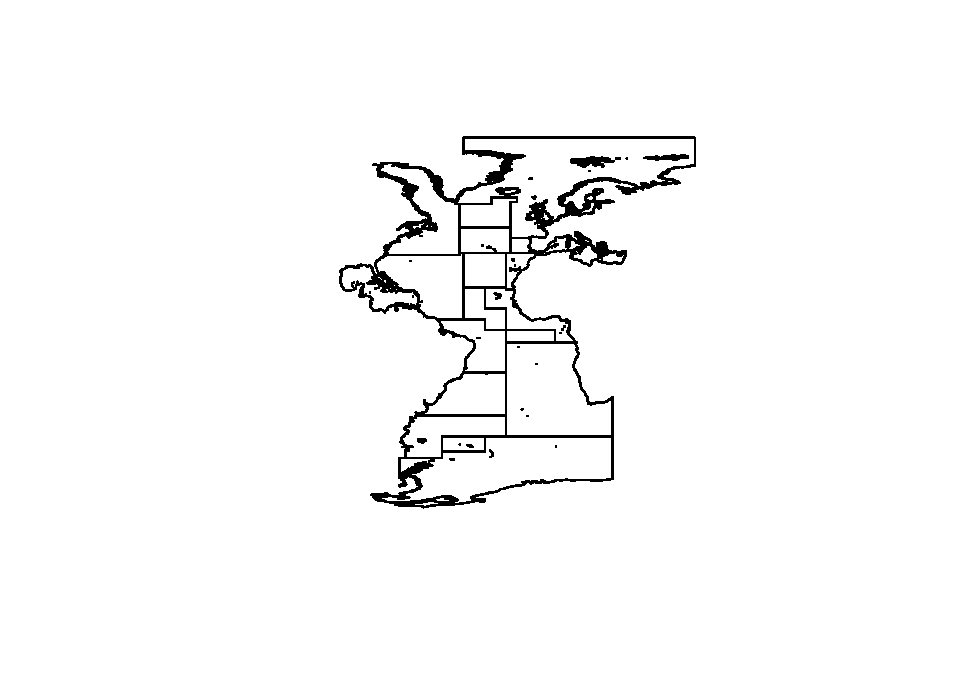
\includegraphics{_main_files/figure-latex/unnamed-chunk-4-1.pdf}

\begin{Shaded}
\begin{Highlighting}[]
\CommentTok{\# Remove unused files}
\FunctionTok{rm}\NormalTok{(FAO, FAO\_Atl, FAO\_Atl.sf, FAO\_Atl\_no\_black\_sea, Black\_Sea, Black\_Sea.sf)}
\end{Highlighting}
\end{Shaded}

Download occurrence data from OBIS and GBIF using scientific name.

In this case we select Albacore tuna species (Thunnus alalunga).

\begin{Shaded}
\begin{Highlighting}[]
\CommentTok{\# Get data from OBIS}
\CommentTok{\#mydata.obis\textless{}{-}robis::occurrence(scientificname="Thunnus alalunga")}
\CommentTok{\#save(mydata.obis, file=file.path("data","occurrences",file="mydata.obis.RData"))}
\FunctionTok{load}\NormalTok{(here}\SpecialCharTok{::}\FunctionTok{here}\NormalTok{ (}\StringTok{"data"}\NormalTok{, }\StringTok{"occurrences"}\NormalTok{, }\StringTok{"mydata.obis.RData"}\NormalTok{))}

\CommentTok{\# Get data from GBIF}
\CommentTok{\#mydata.gbif\textless{}{-}occ\_data(scientificName="Thunnus alalunga", hasCoordinate = TRUE, limit=100000)$data}
\CommentTok{\#save(mydata.gbif,file=file.path("data","occurrences",file="mydata.gbif.RData"))}
\FunctionTok{load}\NormalTok{(here}\SpecialCharTok{::}\FunctionTok{here}\NormalTok{ (}\StringTok{"data"}\NormalTok{, }\StringTok{"occurrences"}\NormalTok{, }\StringTok{"mydata.gbif.RData"}\NormalTok{))}
\end{Highlighting}
\end{Shaded}

We now check the downloaded data and select the fields of interest.

\begin{Shaded}
\begin{Highlighting}[]
\CommentTok{\# Check names for GBIF data}
\FunctionTok{names}\NormalTok{(mydata.gbif)}
\end{Highlighting}
\end{Shaded}

\begin{verbatim}
##   [1] "key"                              "scientificName"                  
##   [3] "decimalLatitude"                  "decimalLongitude"                
##   [5] "issues"                           "datasetKey"                      
##   [7] "publishingOrgKey"                 "installationKey"                 
##   [9] "publishingCountry"                "protocol"                        
##  [11] "lastCrawled"                      "lastParsed"                      
##  [13] "crawlId"                          "hostingOrganizationKey"          
##  [15] "basisOfRecord"                    "occurrenceStatus"                
##  [17] "taxonKey"                         "kingdomKey"                      
##  [19] "phylumKey"                        "orderKey"                        
##  [21] "familyKey"                        "genusKey"                        
##  [23] "speciesKey"                       "acceptedTaxonKey"                
##  [25] "acceptedScientificName"           "kingdom"                         
##  [27] "phylum"                           "order"                           
##  [29] "family"                           "genus"                           
##  [31] "species"                          "genericName"                     
##  [33] "specificEpithet"                  "taxonRank"                       
##  [35] "taxonomicStatus"                  "iucnRedListCategory"             
##  [37] "dateIdentified"                   "coordinateUncertaintyInMeters"   
##  [39] "year"                             "month"                           
##  [41] "day"                              "eventDate"                       
##  [43] "modified"                         "lastInterpreted"                 
##  [45] "references"                       "license"                         
##  [47] "isInCluster"                      "datasetName"                     
##  [49] "recordedBy"                       "identifiedBy"                    
##  [51] "geodeticDatum"                    "countryCode"                     
##  [53] "country"                          "rightsHolder"                    
##  [55] "identifier"                       "http://unknown.org/nick"         
##  [57] "informationWithheld"              "verbatimEventDate"               
##  [59] "collectionCode"                   "gbifID"                          
##  [61] "occurrenceID"                     "taxonID"                         
##  [63] "catalogNumber"                    "institutionCode"                 
##  [65] "eventTime"                        "http://unknown.org/captive"      
##  [67] "identificationID"                 "continent"                       
##  [69] "stateProvince"                    "verbatimLocality"                
##  [71] "occurrenceRemarks"                "lifeStage"                       
##  [73] "datasetID"                        "eventID"                         
##  [75] "footprintWKT"                     "originalNameUsage"               
##  [77] "county"                           "identificationVerificationStatus"
##  [79] "nameAccordingTo"                  "networkKeys"                     
##  [81] "individualCount"                  "elevation"                       
##  [83] "waterBody"                        "institutionKey"                  
##  [85] "otherCatalogNumbers"              "preparations"                    
##  [87] "recordNumber"                     "acceptedNameUsage"               
##  [89] "vernacularName"                   "institutionID"                   
##  [91] "language"                         "type"                            
##  [93] "identificationRemarks"            "projectId"                       
##  [95] "municipality"                     "collectionKey"                   
##  [97] "higherGeography"                  "georeferenceProtocol"            
##  [99] "island"                           "endDayOfYear"                    
## [101] "locality"                         "fieldNumber"                     
## [103] "startDayOfYear"                   "collectionID"                    
## [105] "higherClassification"             "materialSampleID"                
## [107] "disposition"                      "programmeAcronym"                
## [109] "organismQuantity"                 "organismQuantityType"            
## [111] "samplingProtocol"                 "locationAccordingTo"             
## [113] "coordinatePrecision"              "georeferencedDate"               
## [115] "nomenclaturalCode"                "associatedReferences"            
## [117] "taxonRemarks"                     "ownerInstitutionCode"            
## [119] "bibliographicCitation"            "habitat"                         
## [121] "locationRemarks"                  "depth"                           
## [123] "http://unknown.org/license"       "taxonConceptID"                  
## [125] "http://unknown.org/rightsHolder"  "depthAccuracy"                   
## [127] "dynamicProperties"                "elevationAccuracy"               
## [129] "rights"                           "georeferenceSources"             
## [131] "georeferenceRemarks"              "name"                            
## [133] "associatedSequences"              "establishmentMeans"              
## [135] "georeferenceVerificationStatus"   "accessRights"                    
## [137] "georeferencedBy"                  "verbatimSRS"                     
## [139] "previousIdentifications"          "locationID"                      
## [141] "acceptedNameUsageID"              "http://unknown.org/language"     
## [143] "http://unknown.org/modified"      "samplingEffort"                  
## [145] "verbatimDepth"                    "behavior"                        
## [147] "eventRemarks"                     "footprintSRS"                    
## [149] "namePublishedInYear"              "verbatimCoordinateSystem"        
## [151] "parentNameUsage"                  "http://unknown.org/taxonRankID"  
## [153] "http://unknown.org/species"       "higherGeographyID"               
## [155] "islandGroup"                      "organismID"                      
## [157] "distanceFromCentroidInMeters"     "http://unknown.org/orders"       
## [159] "typeStatus"
\end{verbatim}

\begin{Shaded}
\begin{Highlighting}[]
\CommentTok{\# Select columns of interest}
\NormalTok{mydata.gbif }\OtherTok{\textless{}{-}}\NormalTok{ mydata.gbif }\SpecialCharTok{\%\textgreater{}\%}
\NormalTok{                dplyr}\SpecialCharTok{::}\FunctionTok{select}\NormalTok{(}\StringTok{"acceptedScientificName"}\NormalTok{,}
                  \StringTok{"decimalLongitude"}\NormalTok{,}
                  \StringTok{"decimalLatitude"}\NormalTok{,}
                  \StringTok{"year"}\NormalTok{,}
                  \StringTok{"month"}\NormalTok{,}
                  \StringTok{"day"}\NormalTok{,}
                  \StringTok{"eventDate"}\NormalTok{,}
                  \StringTok{"depth"}\NormalTok{)}

\CommentTok{\# Check names in for OBIS data}
\FunctionTok{names}\NormalTok{(mydata.obis)}
\end{Highlighting}
\end{Shaded}

\begin{verbatim}
##   [1] "infraphylum"                    "country"                       
##   [3] "date_year"                      "scientificNameID"              
##   [5] "year"                           "scientificName"                
##   [7] "dropped"                        "gigaclassid"                   
##   [9] "aphiaID"                        "decimalLatitude"               
##  [11] "subclassid"                     "gigaclass"                     
##  [13] "infraphylumid"                  "phylumid"                      
##  [15] "familyid"                       "catalogNumber"                 
##  [17] "basisOfRecord"                  "terrestrial"                   
##  [19] "id"                             "day"                           
##  [21] "parvphylum"                     "order"                         
##  [23] "dataset_id"                     "locality"                      
##  [25] "decimalLongitude"               "collectionCode"                
##  [27] "date_end"                       "speciesid"                     
##  [29] "date_start"                     "month"                         
##  [31] "genus"                          "eventDate"                     
##  [33] "brackish"                       "absence"                       
##  [35] "subfamily"                      "genusid"                       
##  [37] "originalScientificName"         "marine"                        
##  [39] "subphylumid"                    "subfamilyid"                   
##  [41] "institutionCode"                "date_mid"                      
##  [43] "class"                          "orderid"                       
##  [45] "waterBody"                      "kingdom"                       
##  [47] "classid"                        "phylum"                        
##  [49] "species"                        "subphylum"                     
##  [51] "subclass"                       "family"                        
##  [53] "category"                       "kingdomid"                     
##  [55] "parvphylumid"                   "node_id"                       
##  [57] "flags"                          "sss"                           
##  [59] "shoredistance"                  "sst"                           
##  [61] "bathymetry"                     "maximumDepthInMeters"          
##  [63] "minimumDepthInMeters"           "sex"                           
##  [65] "depth"                          "coordinatePrecision"           
##  [67] "verbatimCoordinates"            "occurrenceRemarks"             
##  [69] "individualCount"                "occurrenceStatus"              
##  [71] "modified"                       "materialSampleID"              
##  [73] "occurrenceID"                   "scientificNameAuthorship"      
##  [75] "taxonRank"                      "datasetID"                     
##  [77] "associatedReferences"           "bibliographicCitation"         
##  [79] "coordinateUncertaintyInMeters"  "vernacularName"                
##  [81] "footprintWKT"                   "specificEpithet"               
##  [83] "recordNumber"                   "georeferenceRemarks"           
##  [85] "stateProvince"                  "continent"                     
##  [87] "recordedBy"                     "rightsHolder"                  
##  [89] "language"                       "type"                          
##  [91] "license"                        "ownerInstitutionCode"          
##  [93] "datasetName"                    "geodeticDatum"                 
##  [95] "accessRights"                   "dynamicProperties"             
##  [97] "county"                         "samplingEffort"                
##  [99] "lifeStage"                      "footprintSRS"                  
## [101] "samplingProtocol"               "parentEventID"                 
## [103] "eventID"                        "eventRemarks"                  
## [105] "identifiedBy"                   "georeferencedBy"               
## [107] "minimumElevationInMeters"       "maximumElevationInMeters"      
## [109] "dateIdentified"                 "behavior"                      
## [111] "georeferenceProtocol"           "verbatimDepth"                 
## [113] "organismQuantity"               "organismQuantityType"          
## [115] "startDayOfYear"                 "collectionID"                  
## [117] "typeStatus"                     "institutionID"                 
## [119] "acceptedNameUsage"              "preparations"                  
## [121] "countryCode"                    "otherCatalogNumbers"           
## [123] "references"                     "fieldNumber"                   
## [125] "endDayOfYear"                   "eventTime"                     
## [127] "locationID"                     "taxonRemarks"                  
## [129] "georeferencedDate"              "verbatimEventDate"             
## [131] "identificationRemarks"          "nomenclaturalCode"             
## [133] "taxonomicStatus"                "higherClassification"          
## [135] "higherGeography"                "verbatimLatitude"              
## [137] "verbatimLongitude"              "establishmentMeans"            
## [139] "verbatimLocality"               "georeferenceVerificationStatus"
## [141] "island"                         "identificationQualifier"       
## [143] "identificationID"               "informationWithheld"           
## [145] "islandGroup"                    "acceptedNameUsageID"           
## [147] "locationRemarks"                "verbatimSRS"                   
## [149] "previousIdentifications"
\end{verbatim}

\begin{Shaded}
\begin{Highlighting}[]
\CommentTok{\# Select columns of interest}
\NormalTok{mydata.obis }\OtherTok{\textless{}{-}}\NormalTok{  mydata.obis }\SpecialCharTok{\%\textgreater{}\%}
\NormalTok{                dplyr}\SpecialCharTok{::}\FunctionTok{select}\NormalTok{(}\StringTok{"scientificName"}\NormalTok{,}
                  \StringTok{"decimalLongitude"}\NormalTok{,}
                  \StringTok{"decimalLatitude"}\NormalTok{,}
                  \StringTok{"date\_year"}\NormalTok{,}
                  \StringTok{"month"}\NormalTok{,}
                  \StringTok{"day"}\NormalTok{,}
                  \StringTok{"eventDate"}\NormalTok{,}
                  \StringTok{"depth"}\NormalTok{,}
                  \StringTok{"bathymetry"}\NormalTok{,}
                  \StringTok{"occurrenceStatus"}\NormalTok{,}
                  \StringTok{"sst"}\NormalTok{)}
\end{Highlighting}
\end{Shaded}

Reformat the data adding a new field and renaming some columns from mydata.gbif dataframe in order to have the same columns and be able to join both downloaded datasets.

\begin{Shaded}
\begin{Highlighting}[]
\NormalTok{mydata.gbif }\OtherTok{\textless{}{-}}\NormalTok{ mydata.gbif }\SpecialCharTok{\%\textgreater{}\%} 
\NormalTok{    dplyr}\SpecialCharTok{::}\FunctionTok{rename}\NormalTok{(}\AttributeTok{scientificName=} \StringTok{"acceptedScientificName"}\NormalTok{) }\SpecialCharTok{\%\textgreater{}\%} 
\NormalTok{    dplyr}\SpecialCharTok{::}\FunctionTok{rename}\NormalTok{(}\AttributeTok{date\_year =} \StringTok{"year"}\NormalTok{) }\SpecialCharTok{\%\textgreater{}\%} 
\NormalTok{    dplyr}\SpecialCharTok{::}\FunctionTok{mutate}\NormalTok{(}\AttributeTok{bathymetry=} \ConstantTok{NA}\NormalTok{) }\SpecialCharTok{\%\textgreater{}\%} 
\NormalTok{    dplyr}\SpecialCharTok{::}\FunctionTok{mutate}\NormalTok{(}\AttributeTok{occurrenceStatus=}\DecValTok{1}\NormalTok{) }\SpecialCharTok{\%\textgreater{}\%} 
\NormalTok{    dplyr}\SpecialCharTok{::}\FunctionTok{mutate}\NormalTok{(}\AttributeTok{sst=} \ConstantTok{NA}\NormalTok{)}

\CommentTok{\# Join data from OBIS and GBIF }
\NormalTok{mydata.fus}\OtherTok{\textless{}{-}}\FunctionTok{rbind}\NormalTok{(mydata.obis,mydata.gbif)}
  
\CommentTok{\# Assign unique scientific name }
\NormalTok{mydata.fus }\OtherTok{\textless{}{-}}\NormalTok{ mydata.fus }\SpecialCharTok{\%\textgreater{}\%} 
\NormalTok{    dplyr}\SpecialCharTok{::}\FunctionTok{mutate}\NormalTok{(}\AttributeTok{scientificName=} \FunctionTok{paste}\NormalTok{(mydata.obis}\SpecialCharTok{$}\NormalTok{scientificName[}\DecValTok{1}\NormalTok{]))}

\CommentTok{\# Remove unused files}
\FunctionTok{rm}\NormalTok{(mydata.gbif, mydata.obis)}
\end{Highlighting}
\end{Shaded}

We now clean downloaded raw data.

\begin{Shaded}
\begin{Highlighting}[]
\CommentTok{\# Give date format to eventDate and fill out month and date\_year columns}
\NormalTok{  mydata.fus}\SpecialCharTok{$}\NormalTok{eventDate }\OtherTok{\textless{}{-}} \FunctionTok{as.Date}\NormalTok{(mydata.fus}\SpecialCharTok{$}\NormalTok{eventDate)}
\NormalTok{  mydata.fus}\SpecialCharTok{$}\NormalTok{date\_year }\OtherTok{\textless{}{-}} \FunctionTok{as.numeric}\NormalTok{(mydata.fus}\SpecialCharTok{$}\NormalTok{date\_year)}
\NormalTok{  mydata.fus}\SpecialCharTok{$}\NormalTok{month }\OtherTok{\textless{}{-}} \FunctionTok{as.numeric}\NormalTok{(mydata.fus}\SpecialCharTok{$}\NormalTok{month)}

\CommentTok{\# Mutate occurrenceStatus column giving them a value of 1}
\FunctionTok{unique}\NormalTok{ (mydata.fus}\SpecialCharTok{$}\NormalTok{occurrenceStatus)}
\end{Highlighting}
\end{Shaded}

\begin{verbatim}
## [1] NA        "present" "P"       "Present" "NA"      "1"
\end{verbatim}

\begin{Shaded}
\begin{Highlighting}[]
\CommentTok{\# Assign 1 value to all occurrences}
\NormalTok{mydata.fus }\OtherTok{\textless{}{-}}\NormalTok{ mydata.fus  }\SpecialCharTok{\%\textgreater{}\%} 
\NormalTok{    dplyr}\SpecialCharTok{::}\FunctionTok{mutate}\NormalTok{(}\AttributeTok{occurrenceStatus =} \DecValTok{1}\NormalTok{)}
\end{Highlighting}
\end{Shaded}

We remove outliers based on distance method (total distance= 1000 km).

\begin{Shaded}
\begin{Highlighting}[]
\NormalTok{out.dist }\OtherTok{\textless{}{-}} \FunctionTok{cc\_outl}\NormalTok{(}\AttributeTok{x=}\NormalTok{mydata.fus,}
                \AttributeTok{lon =} \StringTok{"decimalLongitude"}\NormalTok{, }\AttributeTok{lat =} \StringTok{"decimalLatitude"}\NormalTok{,}
                \AttributeTok{species =} \StringTok{"scientificName"}\NormalTok{,}
                \AttributeTok{method=}\StringTok{"distance"}\NormalTok{, }\AttributeTok{tdi=}\DecValTok{1000}\NormalTok{, }\CommentTok{\# distance method with tdi=1000km}
                \AttributeTok{thinning=}\NormalTok{T, }\AttributeTok{thinning\_res=}\FloatTok{0.5}\NormalTok{,}
                \AttributeTok{value=}\StringTok{"flagged"}\NormalTok{) }

\CommentTok{\# Remove outliers from the data}
\NormalTok{mydata.fus }\OtherTok{\textless{}{-}}\NormalTok{ mydata.fus[out.dist, ]}
\end{Highlighting}
\end{Shaded}

Remove duplicates.

\begin{Shaded}
\begin{Highlighting}[]
\CommentTok{\# First create a vector containing longitude, latitude and event date information}
\NormalTok{date }\OtherTok{\textless{}{-}} \FunctionTok{cbind}\NormalTok{(mydata.fus}\SpecialCharTok{$}\NormalTok{decimalLongitude,mydata.fus}\SpecialCharTok{$}\NormalTok{decimalLatitude,mydata.fus}\SpecialCharTok{$}\NormalTok{eventDate)}

\CommentTok{\# Remove the duplicated records}
\NormalTok{mydata.fus}\OtherTok{\textless{}{-}}\NormalTok{mydata.fus[}\SpecialCharTok{!}\FunctionTok{duplicated}\NormalTok{(date),]}

\CommentTok{\# Remove unused files}
\FunctionTok{rm}\NormalTok{(date)}
\end{Highlighting}
\end{Shaded}

Mask retrieved occurrence data to our study area and add bathymetry value to each occurrence point.

\begin{Shaded}
\begin{Highlighting}[]
\CommentTok{\# Assign coordinate format and projection to be able to use FAO Atlantic as a mask}
\NormalTok{dat }\OtherTok{\textless{}{-}} \FunctionTok{data.frame}\NormalTok{(}\FunctionTok{cbind}\NormalTok{(mydata.fus}\SpecialCharTok{$}\NormalTok{decimalLongitude,mydata.fus}\SpecialCharTok{$}\NormalTok{decimalLatitude))}
\NormalTok{ptos}\OtherTok{\textless{}{-}}\FunctionTok{as.data.table}\NormalTok{(dat,}\AttributeTok{keep.columnnames=}\ConstantTok{TRUE}\NormalTok{)}
  
\FunctionTok{coordinates}\NormalTok{(ptos) }\OtherTok{\textless{}{-}} \ErrorTok{\textasciitilde{}}\NormalTok{ X1 }\SpecialCharTok{+}\NormalTok{ X2}

\CommentTok{\# Assign projection}
\FunctionTok{proj4string}\NormalTok{(ptos) }\OtherTok{\textless{}{-}}\FunctionTok{proj4string}\NormalTok{(study\_area)}
  
\CommentTok{\# Select only occurrences from FAO Atlantic}

\NormalTok{match2}\OtherTok{\textless{}{-}}\FunctionTok{data.frame}\NormalTok{(}\FunctionTok{subset}\NormalTok{(mydata.fus,}\SpecialCharTok{!}\FunctionTok{is.na}\NormalTok{(}\FunctionTok{over}\NormalTok{(ptos, study\_area)[,}\DecValTok{1}\NormalTok{])))}
  
\CommentTok{\# Extract the FAO area of each point}
\NormalTok{match3}\OtherTok{\textless{}{-}}\FunctionTok{data.frame}\NormalTok{(}\FunctionTok{subset}\NormalTok{(}\FunctionTok{over}\NormalTok{(ptos, study\_area), }\SpecialCharTok{!}\FunctionTok{is.na}\NormalTok{(}\FunctionTok{over}\NormalTok{(ptos, study\_area)[,}\DecValTok{1}\NormalTok{])))}
  
\CommentTok{\# Create data frame with area, name, long, lat and year }
\NormalTok{df0}\OtherTok{\textless{}{-}}\FunctionTok{cbind}\NormalTok{(}\AttributeTok{F\_AREA=}\NormalTok{match3}\SpecialCharTok{$}\NormalTok{F\_AREA,match2)[,}\FunctionTok{c}\NormalTok{(}\StringTok{"F\_AREA"}\NormalTok{,}\StringTok{"scientificName"}\NormalTok{,}\StringTok{"decimalLongitude"}\NormalTok{,}\StringTok{"decimalLatitude"}\NormalTok{,}\StringTok{"date\_year"}\NormalTok{,}\StringTok{"occurrenceStatus"}\NormalTok{)]}

\CommentTok{\# Rename some columns}
\FunctionTok{names}\NormalTok{(df0)[}\DecValTok{3}\SpecialCharTok{:}\DecValTok{5}\NormalTok{]}\OtherTok{\textless{}{-}}\FunctionTok{c}\NormalTok{(}\StringTok{"LON"}\NormalTok{,}\StringTok{"LAT"}\NormalTok{,}\StringTok{"YEAR"}\NormalTok{)}

\CommentTok{\# Add bathymetry from NOAA}
\CommentTok{\#bathy \textless{}{-} marmap::getNOAA.bathy(lon1={-}100,lon2=30,lat1={-}41,lat2=55, resolution = 1,               keep=TRUE, antimeridian=FALSE, path= here::here("data", "spatial"))}
\FunctionTok{load}\NormalTok{(here}\SpecialCharTok{::}\FunctionTok{here}\NormalTok{ (}\StringTok{"data"}\NormalTok{, }\StringTok{"spatial"}\NormalTok{, }\StringTok{"bathy.RData"}\NormalTok{))}

\NormalTok{df0}\SpecialCharTok{$}\NormalTok{bathymetry }\OtherTok{\textless{}{-}} \FunctionTok{get.depth}\NormalTok{(bathy, df0[,}\FunctionTok{c}\NormalTok{(}\StringTok{"LON"}\NormalTok{,}\StringTok{"LAT"}\NormalTok{)], }\AttributeTok{locator=}\NormalTok{F)}\SpecialCharTok{$}\NormalTok{depth}

\CommentTok{\# Remove unused files}
\FunctionTok{rm}\NormalTok{(mydata.fus, match2, match3, dat, ptos)}
\end{Highlighting}
\end{Shaded}

We plot the occurrence data.

\begin{Shaded}
\begin{Highlighting}[]
\FunctionTok{ggplot}\NormalTok{() }\SpecialCharTok{+}
   \FunctionTok{geom\_path}\NormalTok{(}\AttributeTok{data =}\NormalTok{ study\_area, }
             \FunctionTok{aes}\NormalTok{(}\AttributeTok{x =}\NormalTok{ long, }\AttributeTok{y =}\NormalTok{ lat, }\AttributeTok{group =}\NormalTok{ group),}
             \AttributeTok{color =} \StringTok{\textquotesingle{}gray\textquotesingle{}}\NormalTok{, }\AttributeTok{linewidth =}\NormalTok{ .}\DecValTok{2}\NormalTok{) }\SpecialCharTok{+}
   \FunctionTok{geom\_point}\NormalTok{(}\AttributeTok{data=}\NormalTok{df0, }\FunctionTok{aes}\NormalTok{(}\AttributeTok{x=}\NormalTok{LON, }\AttributeTok{y=}\NormalTok{LAT)) }
\end{Highlighting}
\end{Shaded}

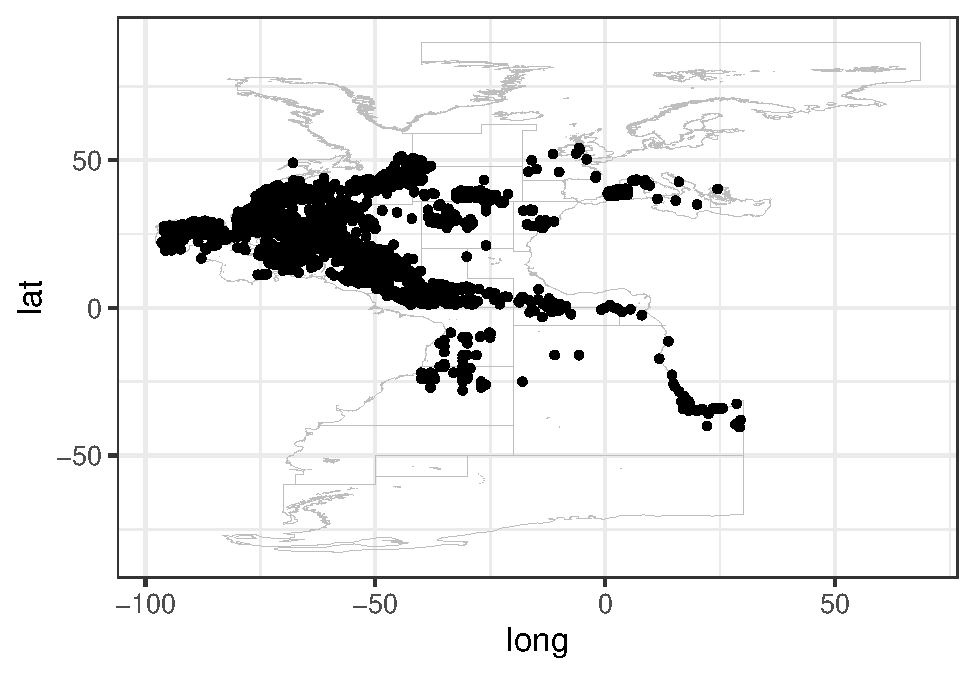
\includegraphics{_main_files/figure-latex/unnamed-chunk-12-1.pdf}

And, we save the data.

\begin{Shaded}
\begin{Highlighting}[]
\FunctionTok{save}\NormalTok{(df0, }\AttributeTok{file =} \StringTok{"data/occurrences/occ.RData"}\NormalTok{)}
\FunctionTok{save}\NormalTok{(study\_area, }\AttributeTok{file =} \StringTok{"data/spatial/study\_area.RData"}\NormalTok{)}
\end{Highlighting}
\end{Shaded}

\hypertarget{create-pseudo-absence-data}{%
\section{Create pseudo-absence data}\label{create-pseudo-absence-data}}

After saving presence data for the species of interest we need to generate absence data (with a constant prevalence of 50\%, \citet{mcpherson_2004},\citet{barbetmassin_etal_2012}), in order to work with logistic regression SDM afterwards. For that, we generate a buffer around each presence data point, with a radius of 100km, where no absences can be generated.

Before starting the pseudo-absence generation process, we delete observations in land (positive bathymetry) and select data between 2000 and 2014 (same temporal range as the environmental data that we will load later).

\begin{Shaded}
\begin{Highlighting}[]
\CommentTok{\#remove points in land}
\NormalTok{df0}\OtherTok{\textless{}{-}}\FunctionTok{subset}\NormalTok{(df0,bathymetry}\SpecialCharTok{\textless{}}\DecValTok{0}\NormalTok{)}

\CommentTok{\#use years from 2000 to 2014}
\NormalTok{df0}\OtherTok{\textless{}{-}} \FunctionTok{subset}\NormalTok{(df0, YEAR}\SpecialCharTok{\textless{}=}\DecValTok{2014} \SpecialCharTok{\&}\NormalTok{ YEAR}\SpecialCharTok{\textgreater{}=}\DecValTok{2000}\NormalTok{)}
\end{Highlighting}
\end{Shaded}

Then we transform the presence data frame to ``SpatialPointsDataFrame'' class object and the to ``sf'' class object so we can operate and plot easily with spatial data. We can see the characteristics of this object through its summary.

\begin{Shaded}
\begin{Highlighting}[]
\CommentTok{\#convert to spatial point data frame}
\NormalTok{df}\OtherTok{\textless{}{-}}\NormalTok{df0 ; }\FunctionTok{coordinates}\NormalTok{(df)}\OtherTok{\textless{}{-}} \ErrorTok{\textasciitilde{}}\NormalTok{LON}\SpecialCharTok{+}\NormalTok{LAT}
\FunctionTok{crs}\NormalTok{(df)}\OtherTok{\textless{}{-}}\FunctionTok{crs}\NormalTok{(study\_area)}

\CommentTok{\#convert to sf}
\NormalTok{study\_area.sf}\OtherTok{\textless{}{-}}\FunctionTok{st\_union}\NormalTok{(}\FunctionTok{st\_as\_sf}\NormalTok{(study\_area))}
\NormalTok{df.sf}\OtherTok{\textless{}{-}}\FunctionTok{st\_as\_sf}\NormalTok{(df)}

\FunctionTok{summary}\NormalTok{(df)}
\end{Highlighting}
\end{Shaded}

\begin{verbatim}
## Object of class SpatialPointsDataFrame
## Coordinates:
##        min      max
## LON -95.65 24.45000
## LAT -34.71 54.15014
## Is projected: FALSE 
## proj4string : [+proj=longlat +datum=WGS84 +no_defs]
## Number of points: 14903
## Data attributes:
##     F_AREA          scientificName          YEAR      occurrenceStatus
##  Length:14903       Length:14903       Min.   :2000   Min.   :1       
##  Class :character   Class :character   1st Qu.:2001   1st Qu.:1       
##  Mode  :character   Mode  :character   Median :2002   Median :1       
##                                        Mean   :2003   Mean   :1       
##                                        3rd Qu.:2004   3rd Qu.:1       
##                                        Max.   :2013   Max.   :1       
##    bathymetry      
##  Min.   :-8404.09  
##  1st Qu.:-1916.92  
##  Median :-1030.77  
##  Mean   :-1433.61  
##  3rd Qu.: -351.32  
##  Max.   :   -1.13
\end{verbatim}

We can easily plot sf objects using ggplot, here we plot the area of study and the presence data points.

\begin{Shaded}
\begin{Highlighting}[]
\FunctionTok{ggplot}\NormalTok{(study\_area.sf) }\SpecialCharTok{+} 
  \FunctionTok{geom\_sf}\NormalTok{() }\SpecialCharTok{+} 
  \FunctionTok{geom\_sf}\NormalTok{(}\AttributeTok{data=}\FunctionTok{st\_union}\NormalTok{(df.sf),}
          \AttributeTok{size=}\DecValTok{1}\NormalTok{,}
          \AttributeTok{alpha=}\FloatTok{0.5}\NormalTok{)}
\end{Highlighting}
\end{Shaded}

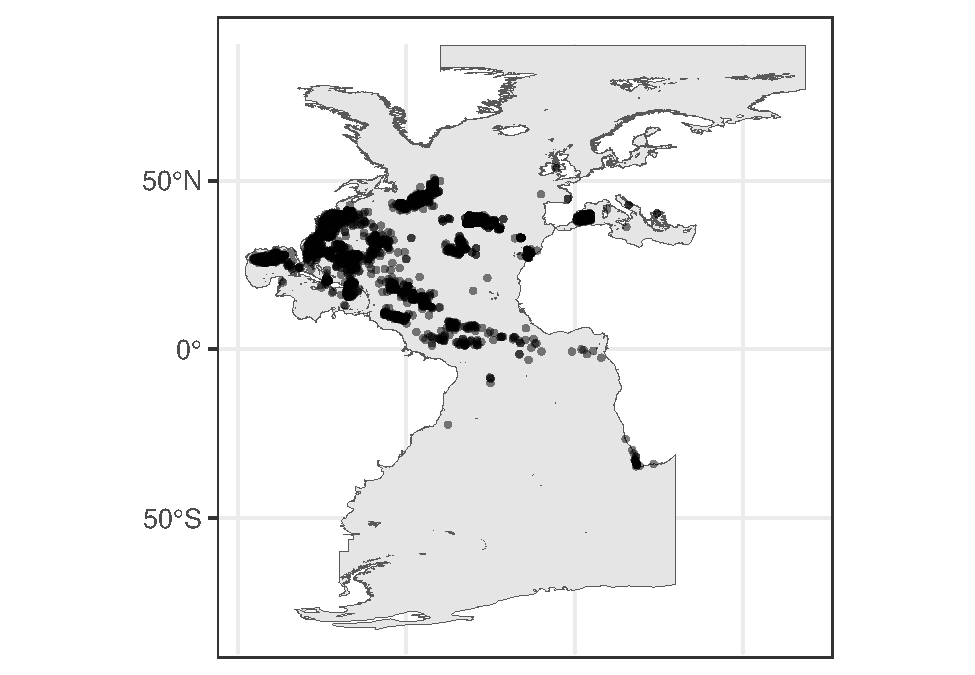
\includegraphics{_main_files/figure-latex/unnamed-chunk-16-1.pdf}

We save a base plot (p0) with the world map and our area of study in blue.

\begin{Shaded}
\begin{Highlighting}[]
\CommentTok{\# basic ggplot}
\NormalTok{global }\OtherTok{\textless{}{-}} \FunctionTok{map\_data}\NormalTok{(}\StringTok{"worldHires"}\NormalTok{)}

\NormalTok{p0 }\OtherTok{\textless{}{-}} \FunctionTok{ggplot}\NormalTok{() }\SpecialCharTok{+} 
  \FunctionTok{annotation\_map}\NormalTok{(}\AttributeTok{map=}\NormalTok{global, }\AttributeTok{fill=}\StringTok{"grey"}\NormalTok{)}\SpecialCharTok{+}
  \FunctionTok{geom\_sf}\NormalTok{(}\AttributeTok{data=}\NormalTok{study\_area.sf,}\AttributeTok{fill=}\DecValTok{5}\NormalTok{)}

\FunctionTok{print}\NormalTok{(p0)}
\end{Highlighting}
\end{Shaded}

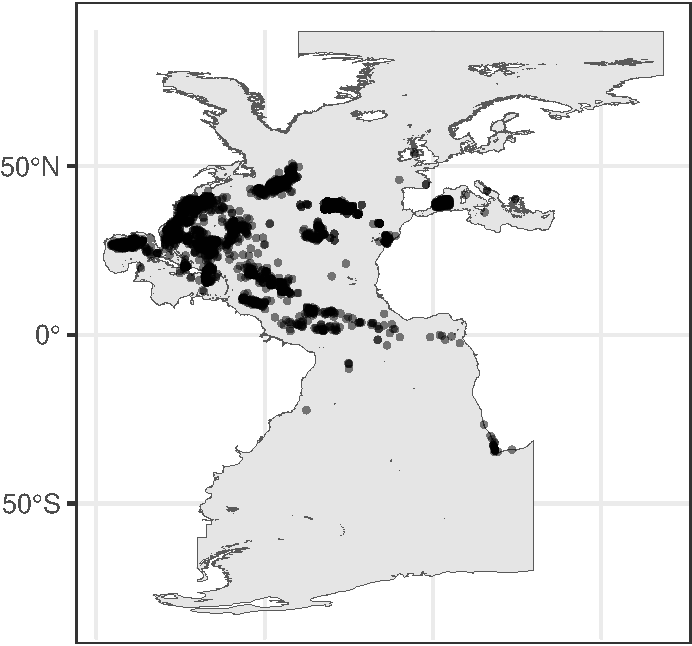
\includegraphics{_main_files/figure-latex/unnamed-chunk-17-1.pdf}

In order to generate a buffer around each occurrence data point, we need to work with euclidean distances, so first, we need to transform the decimal latitude and longitude values to UTM.

\begin{Shaded}
\begin{Highlighting}[]
\CommentTok{\# function to find your UTM. }
\NormalTok{lonlat2UTM }\OtherTok{=} \ControlFlowTok{function}\NormalTok{(lonlat) \{}
\NormalTok{  utm }\OtherTok{=}\NormalTok{ (}\FunctionTok{floor}\NormalTok{((lonlat[}\DecValTok{1}\NormalTok{] }\SpecialCharTok{+} \DecValTok{180}\NormalTok{) }\SpecialCharTok{/} \DecValTok{6}\NormalTok{) }\SpecialCharTok{\%\%} \DecValTok{60}\NormalTok{) }\SpecialCharTok{+} \DecValTok{1}
  \ControlFlowTok{if}\NormalTok{(lonlat[}\DecValTok{2}\NormalTok{] }\SpecialCharTok{\textgreater{}} \DecValTok{0}\NormalTok{) \{}
\NormalTok{    utm }\SpecialCharTok{+} \DecValTok{32600}
\NormalTok{  \} }\ControlFlowTok{else}\NormalTok{\{}
\NormalTok{    utm }\SpecialCharTok{+} \DecValTok{32700}
\NormalTok{  \}}
\NormalTok{\}}

\NormalTok{(EPSG\_2\_UTM }\OtherTok{\textless{}{-}} \FunctionTok{lonlat2UTM}\NormalTok{(}\FunctionTok{c}\NormalTok{(}\FunctionTok{mean}\NormalTok{(df}\SpecialCharTok{$}\NormalTok{LON), }\FunctionTok{mean}\NormalTok{(df}\SpecialCharTok{$}\NormalTok{LAT))))}
\end{Highlighting}
\end{Shaded}

\begin{verbatim}
## [1] 32623
\end{verbatim}

\begin{Shaded}
\begin{Highlighting}[]
\CommentTok{\# transform study\_area and data points to UTMs (in m)}
\NormalTok{aux }\OtherTok{\textless{}{-}} \FunctionTok{st\_transform}\NormalTok{(study\_area.sf, EPSG\_2\_UTM)}
\NormalTok{df.sf.utm }\OtherTok{\textless{}{-}} \FunctionTok{st\_transform}\NormalTok{(df.sf, EPSG\_2\_UTM)}
\end{Highlighting}
\end{Shaded}

Now, we can create buffers of 100 km around the points and join the resulting polygons. Then this buffer is intersected with the area of study defining the area where the pseudo-absences can be generated. To visualize the defined areas, we plot the buffers in red and the area that we will use to generate pseudo-absences in green.

\begin{Shaded}
\begin{Highlighting}[]
\CommentTok{\# create buffers of 100000m}
\NormalTok{buffer }\OtherTok{\textless{}{-}} \FunctionTok{st\_buffer}\NormalTok{(df.sf.utm, }\AttributeTok{dist=}\DecValTok{100000}\NormalTok{)}
\NormalTok{buffer }\OtherTok{\textless{}{-}} \FunctionTok{st\_union}\NormalTok{(buffer)}

\CommentTok{\# intersect the are with the buffer}
\NormalTok{aux0 }\OtherTok{\textless{}{-}} \FunctionTok{st\_difference}\NormalTok{(aux, buffer)}

\CommentTok{\# ggplot for all data}
\NormalTok{p0 }\SpecialCharTok{+}
  \FunctionTok{geom\_sf}\NormalTok{(}\AttributeTok{data=}\NormalTok{aux0,}\AttributeTok{fill=}\DecValTok{3}\NormalTok{) }\SpecialCharTok{+}
  \FunctionTok{geom\_sf}\NormalTok{(}\AttributeTok{data=}\NormalTok{buffer,}\AttributeTok{fill=}\DecValTok{2}\NormalTok{)}
\end{Highlighting}
\end{Shaded}

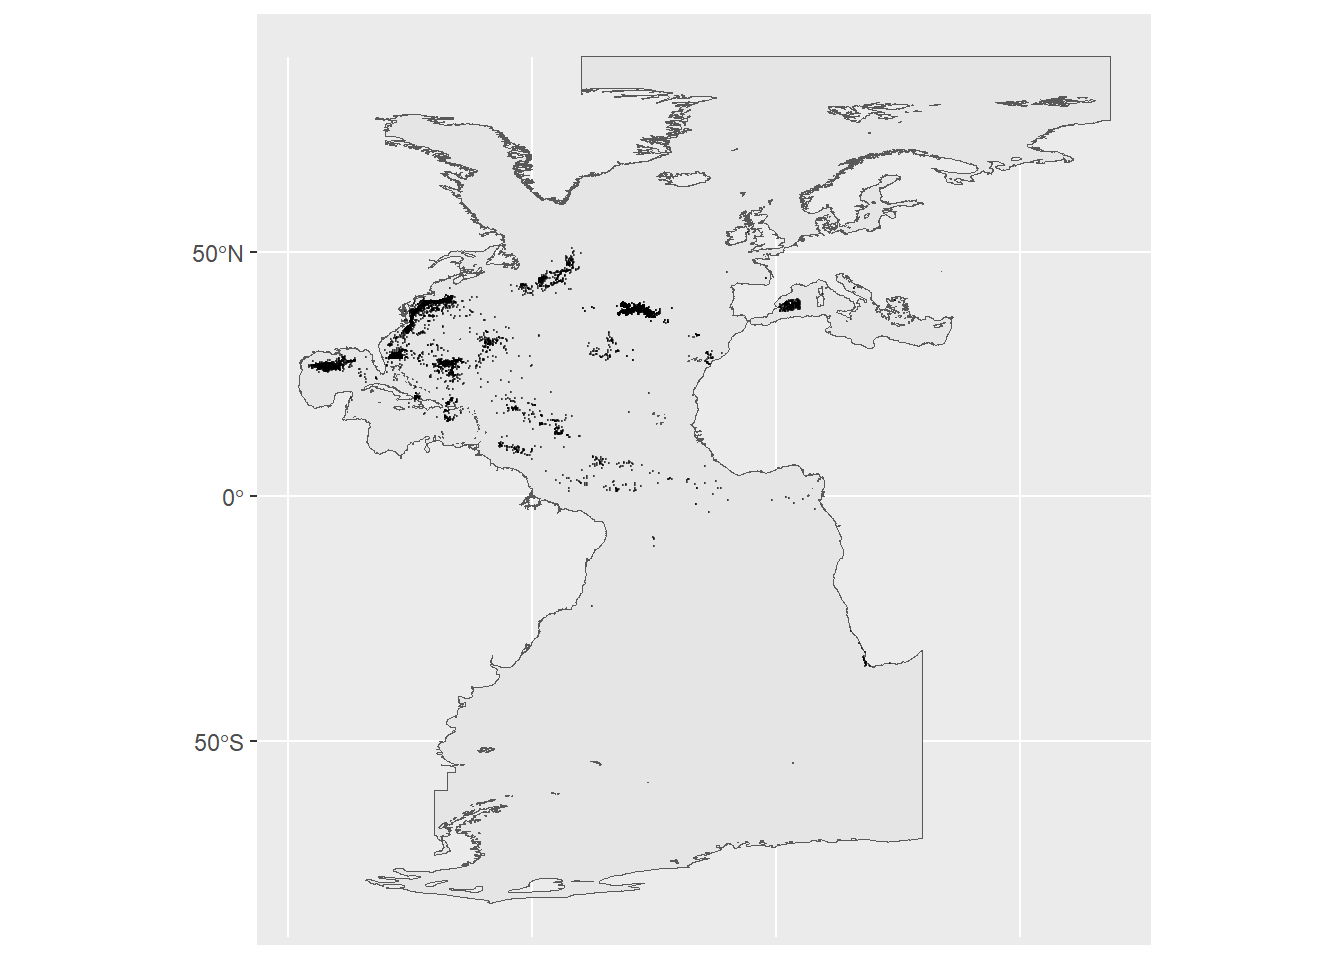
\includegraphics{_main_files/figure-latex/unnamed-chunk-19-1.pdf}

\begin{Shaded}
\begin{Highlighting}[]
\CommentTok{\#zoom}
\NormalTok{p0 }\SpecialCharTok{+}
  \FunctionTok{geom\_sf}\NormalTok{(}\AttributeTok{data=}\NormalTok{aux0,}\AttributeTok{fill=}\DecValTok{3}\NormalTok{) }\SpecialCharTok{+}
  \FunctionTok{geom\_sf}\NormalTok{(}\AttributeTok{data=}\NormalTok{buffer,}\AttributeTok{fill=}\DecValTok{2}\NormalTok{)}\SpecialCharTok{+}
  \FunctionTok{coord\_sf}\NormalTok{(}\AttributeTok{xlim=}\FunctionTok{c}\NormalTok{(}\SpecialCharTok{{-}}\DecValTok{95}\NormalTok{,}\SpecialCharTok{{-}}\DecValTok{82}\NormalTok{), }\AttributeTok{ylim=}\FunctionTok{c}\NormalTok{(}\DecValTok{22}\NormalTok{,}\DecValTok{31}\NormalTok{))}
\end{Highlighting}
\end{Shaded}

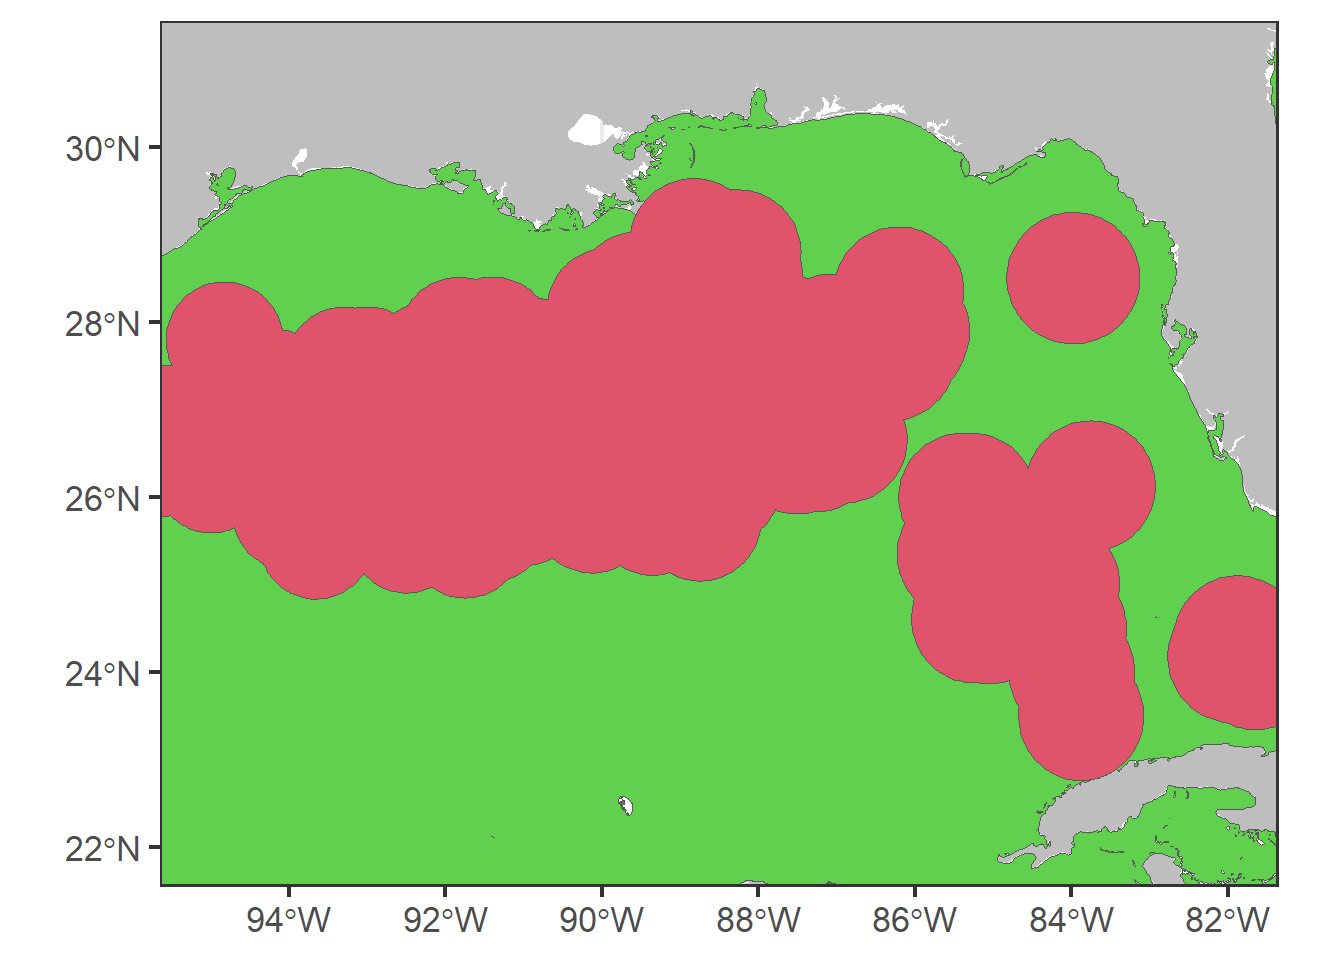
\includegraphics{_main_files/figure-latex/unnamed-chunk-19-2.pdf}

We create a data frame for pseudo-absences with the same dimensions as the presences data frame.

\begin{Shaded}
\begin{Highlighting}[]
\CommentTok{\# Generate the pseudo{-}absence data frame}
\NormalTok{pseudo }\OtherTok{\textless{}{-}} \FunctionTok{matrix}\NormalTok{(}\AttributeTok{data=}\ConstantTok{NA}\NormalTok{, }\AttributeTok{nrow=}\FunctionTok{dim}\NormalTok{(df0)[}\DecValTok{1}\NormalTok{], }\AttributeTok{ncol=}\FunctionTok{dim}\NormalTok{(df0)[}\DecValTok{2}\NormalTok{])}
\NormalTok{pseudo }\OtherTok{\textless{}{-}} \FunctionTok{data.frame}\NormalTok{(pseudo)}
\FunctionTok{names}\NormalTok{(pseudo) }\OtherTok{\textless{}{-}} \FunctionTok{names}\NormalTok{(df0)}
\end{Highlighting}
\end{Shaded}

To generate the pseudo-absence data points, we sample randomly from the defined area and we extract their latitude and longitude to incorporate them in the created data frame. We set the occurrenceStatus equal to 0 as they are absences.

\begin{Shaded}
\begin{Highlighting}[]
\CommentTok{\# set the seed}
\FunctionTok{set.seed}\NormalTok{(}\DecValTok{1}\NormalTok{)}

\CommentTok{\#sample from the defined area}
\NormalTok{rp.sf }\OtherTok{\textless{}{-}} \FunctionTok{st\_sample}\NormalTok{(aux0, }\AttributeTok{size=}\FunctionTok{dim}\NormalTok{(df.sf.utm)[}\DecValTok{1}\NormalTok{], }\AttributeTok{type=}\StringTok{"random"}\NormalTok{) }\CommentTok{\# randomly sample points}

\CommentTok{\# transform to lat and lon and extract coordinates as data.frame}
\NormalTok{rp.sf }\OtherTok{\textless{}{-}} \FunctionTok{st\_transform}\NormalTok{(rp.sf, }\DecValTok{4326}\NormalTok{)}
\NormalTok{rp }\OtherTok{\textless{}{-}} \FunctionTok{as.data.frame}\NormalTok{(}\FunctionTok{st\_coordinates}\NormalTok{(rp.sf)) }
\NormalTok{pseudo}\SpecialCharTok{$}\NormalTok{LON }\OtherTok{\textless{}{-}}\NormalTok{ rp}\SpecialCharTok{$}\NormalTok{X}
\NormalTok{pseudo}\SpecialCharTok{$}\NormalTok{LAT }\OtherTok{\textless{}{-}}\NormalTok{ rp}\SpecialCharTok{$}\NormalTok{Y}

\CommentTok{\# complete the rest of columns}
\NormalTok{pseudo}\SpecialCharTok{$}\NormalTok{scientificName }\OtherTok{\textless{}{-}}\NormalTok{ df0}\SpecialCharTok{$}\NormalTok{scientificName}
\NormalTok{pseudo}\SpecialCharTok{$}\NormalTok{occurrenceStatus  }\OtherTok{\textless{}{-}} \DecValTok{0}
\end{Highlighting}
\end{Shaded}

We can plot the generated pseudo-absence data (in pink) in the map, together with the presence data points (in black).

\begin{Shaded}
\begin{Highlighting}[]
\NormalTok{p0 }\SpecialCharTok{+}
  \FunctionTok{geom\_sf}\NormalTok{(}\AttributeTok{data=}\NormalTok{rp.sf, }\AttributeTok{col=}\DecValTok{6}\NormalTok{, }\AttributeTok{shape=}\DecValTok{4}\NormalTok{,}\AttributeTok{size=}\FloatTok{0.5}\NormalTok{)}\SpecialCharTok{+}
  \FunctionTok{geom\_sf}\NormalTok{(}\AttributeTok{data=}\NormalTok{df.sf.utm, }\AttributeTok{col=}\DecValTok{1}\NormalTok{, }\AttributeTok{alpha=}\FloatTok{0.8}\NormalTok{,}\AttributeTok{size=}\FloatTok{0.5}\NormalTok{)}\SpecialCharTok{+}
  \FunctionTok{ggtitle}\NormalTok{(}\FunctionTok{unique}\NormalTok{(df}\SpecialCharTok{$}\NormalTok{scientificName))}
\end{Highlighting}
\end{Shaded}

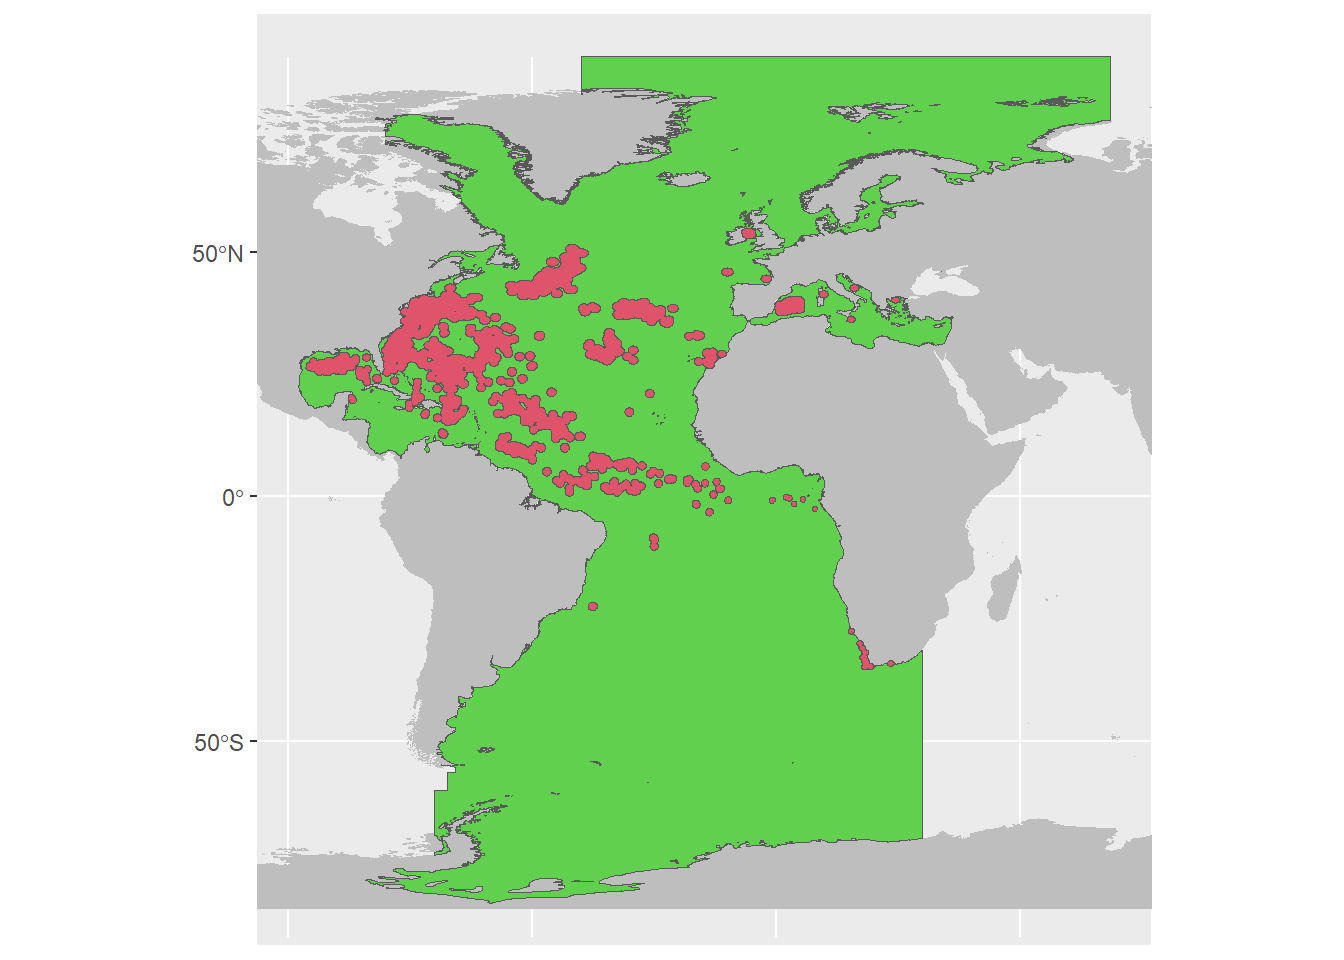
\includegraphics{_main_files/figure-latex/unnamed-chunk-22-1.pdf}

\begin{Shaded}
\begin{Highlighting}[]
\CommentTok{\#zoom}
\NormalTok{p0 }\SpecialCharTok{+}
  \FunctionTok{geom\_sf}\NormalTok{(}\AttributeTok{data=}\NormalTok{rp.sf, }\AttributeTok{col=}\DecValTok{6}\NormalTok{, }\AttributeTok{shape=}\DecValTok{4}\NormalTok{,}\AttributeTok{size=}\DecValTok{1}\NormalTok{)}\SpecialCharTok{+}
  \FunctionTok{geom\_sf}\NormalTok{(}\AttributeTok{data=}\NormalTok{df.sf.utm, }\AttributeTok{col=}\DecValTok{1}\NormalTok{, }\AttributeTok{alpha=}\FloatTok{0.8}\NormalTok{,}\AttributeTok{size=}\FloatTok{0.5}\NormalTok{)}\SpecialCharTok{+}
  \FunctionTok{coord\_sf}\NormalTok{(}\AttributeTok{xlim=}\FunctionTok{c}\NormalTok{(}\SpecialCharTok{{-}}\DecValTok{95}\NormalTok{,}\SpecialCharTok{{-}}\DecValTok{82}\NormalTok{), }\AttributeTok{ylim=}\FunctionTok{c}\NormalTok{(}\DecValTok{23}\NormalTok{,}\DecValTok{31}\NormalTok{))}\SpecialCharTok{+}
  \FunctionTok{ggtitle}\NormalTok{(}\FunctionTok{unique}\NormalTok{(df}\SpecialCharTok{$}\NormalTok{scientificName))}
\end{Highlighting}
\end{Shaded}

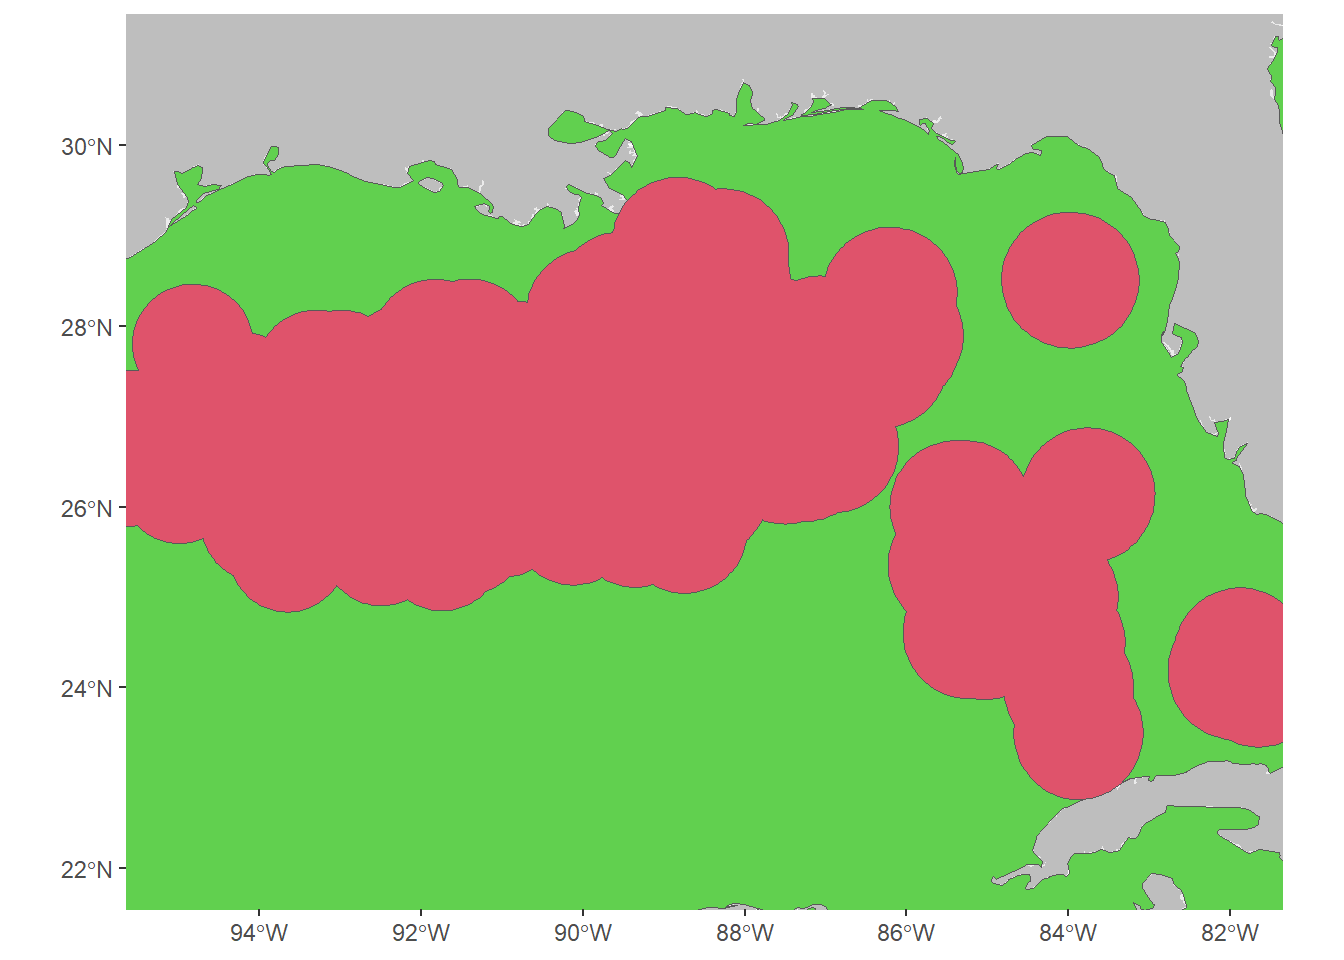
\includegraphics{_main_files/figure-latex/unnamed-chunk-22-2.pdf}

Finally we join the presence and pseudo-absence data frames selecting the columns of interest and save the new data frame as well as the area object.

\begin{Shaded}
\begin{Highlighting}[]
\CommentTok{\# Join the two data sets }
\NormalTok{PAdata }\OtherTok{\textless{}{-}} \FunctionTok{rbind}\NormalTok{(df0, pseudo)[,}\FunctionTok{c}\NormalTok{(}\StringTok{"scientificName"}\NormalTok{,}\StringTok{"LON"}\NormalTok{,}\StringTok{"LAT"}\NormalTok{,}\StringTok{"YEAR"}\NormalTok{,}\StringTok{"occurrenceStatus"}\NormalTok{)]}

\CommentTok{\# Save the final dataset of occurrence and pseudo{-}absence points}
\FunctionTok{save}\NormalTok{(}\AttributeTok{list=}\FunctionTok{c}\NormalTok{(}\StringTok{"PAdata"}\NormalTok{),}\AttributeTok{file=}\FunctionTok{file.path}\NormalTok{(}\StringTok{"data"}\NormalTok{,}\StringTok{"outputs\_for\_modelling"}\NormalTok{,}\AttributeTok{file=}\StringTok{"PAdata.RData"}\NormalTok{))}
\end{Highlighting}
\end{Shaded}

\hypertarget{environmental-data}{%
\chapter{Environmental data}\label{environmental-data}}

In this chapter we first, download environmental data from a public repository; second, we crop the data to our area of interest, and we save it as raster stack.

As in chapter 2, first, we load a list of required libraries.

\begin{Shaded}
\begin{Highlighting}[]
\NormalTok{requiredPackages }\OtherTok{\textless{}{-}} \FunctionTok{c}\NormalTok{(}
  \CommentTok{\#GENERAL USE LIBRARIES {-}{-}{-}{-}{-}{-}{-}{-}\#}
  \StringTok{"here"}\NormalTok{, }\CommentTok{\# Library for reproducible workflow}
  \StringTok{"rstudioapi"}\NormalTok{,  }\CommentTok{\# Library for reproducible workflow}
  \StringTok{"maptools"}\NormalTok{, }\CommentTok{\#plotting world map}
  \StringTok{"ggplot2"}\NormalTok{, }\CommentTok{\#for plotting}
  \StringTok{"knitr"}\NormalTok{,  }\CommentTok{\# format tables}
  \StringTok{"kableExtra"}\NormalTok{, }\CommentTok{\# format tables}
  \StringTok{"raster"}\NormalTok{, }\CommentTok{\# to work with spatial data}
  \StringTok{"dplyr"}\NormalTok{,}
  
  \CommentTok{\#DOWNLOAD FROM PUBLIC REPOSITORIES {-}{-}{-}{-}{-}{-}{-}{-}\#}
  \StringTok{"sdmpredictors"} \CommentTok{\#to access Bio{-}ORACLE dataset}
  
\NormalTok{    )}
\end{Highlighting}
\end{Shaded}

We run a function to install the required packages that are not in our system and load all the required packages.

\begin{Shaded}
\begin{Highlighting}[]
\NormalTok{install\_load\_function }\OtherTok{\textless{}{-}} \ControlFlowTok{function}\NormalTok{(pkg)\{}
\NormalTok{  new.pkg }\OtherTok{\textless{}{-}}\NormalTok{ pkg[}\SpecialCharTok{!}\NormalTok{(pkg }\SpecialCharTok{\%in\%} \FunctionTok{installed.packages}\NormalTok{()[, }\StringTok{"Package"}\NormalTok{])]}
  \ControlFlowTok{if}\NormalTok{ (}\FunctionTok{length}\NormalTok{(new.pkg))}
    \FunctionTok{install.packages}\NormalTok{(new.pkg, }\AttributeTok{dependencies =} \ConstantTok{TRUE}\NormalTok{)}
  \FunctionTok{sapply}\NormalTok{(pkg, require, }\AttributeTok{character.only =} \ConstantTok{TRUE}\NormalTok{)}
\NormalTok{\}}

\FunctionTok{install\_load\_function}\NormalTok{(requiredPackages)}
\end{Highlighting}
\end{Shaded}

\begin{verbatim}
##          here    rstudioapi      maptools       ggplot2         knitr 
##          TRUE          TRUE          TRUE          TRUE          TRUE 
##    kableExtra        raster         dplyr sdmpredictors 
##          TRUE          TRUE          TRUE          TRUE
\end{verbatim}

We define some overall settings.

\begin{Shaded}
\begin{Highlighting}[]
\CommentTok{\# General settings for ggplot (black{-}white background, larger base\_size)}
\FunctionTok{theme\_set}\NormalTok{(}\FunctionTok{theme\_bw}\NormalTok{(}\AttributeTok{base\_size =} \DecValTok{16}\NormalTok{))}
\end{Highlighting}
\end{Shaded}

\hypertarget{download-from-public-repositories}{%
\section{Download from public repositories}\label{download-from-public-repositories}}

Environmental data can be available from different sources. In this case, we used the Bio-ORACLE (ocean
rasters for analyses of climate and environment) database \citep{tyberghein_etal_2012, assis_etal_2017}. These data are publicly available and are easily accessible from the \texttt{sdmpredictors} package \href{https://cran.r-project.org/web/packages/sdmpredictors/index.html}{\texttt{sdmpredictors}}.

We can check the list of available datasets with the function \texttt{list\_datasets} from \texttt{sdmpredictors} package, as follows:

\begin{Shaded}
\begin{Highlighting}[]
\NormalTok{mydat }\OtherTok{\textless{}{-}} \FunctionTok{list\_datasets}\NormalTok{()}

\FunctionTok{kable}\NormalTok{(mydat)}\SpecialCharTok{\%\textgreater{}\%} 
  \FunctionTok{kable\_styling}\NormalTok{(}\StringTok{"striped"}\NormalTok{) }\SpecialCharTok{\%\textgreater{}\%} 
  \FunctionTok{scroll\_box}\NormalTok{(}\AttributeTok{height=}\StringTok{"600px"}\NormalTok{, }\AttributeTok{width =} \StringTok{"100\%"}\NormalTok{)}
\end{Highlighting}
\end{Shaded}

\begin{table}
\centering
\begin{tabular}{l|l|l|l|l|l}
\hline
dataset\_code & terrestrial & marine & url & description & citation\\
\hline
WorldClim & TRUE & FALSE & http://www.worldclim.org/ & WorldClim is a set of global climate layers (climate grids). Note that all data has been transformed back to real values, so there is no need to e.g. divide temperature layers by 10. & Hijmans, R.J., S.E. Cameron, J.L. Parra, P.G. Jones and A. Jarvis, 2005. Very high resolution interpolated climate surfaces for global land areas. International Journal of Climatology 25: 1965-1978.\\
\hline
Bio-ORACLE & FALSE & TRUE & https://bio-oracle.org/ & Bio-ORACLE is a set of GIS rasters providing geophysical, biotic and environmental data for surface and benthic marine realms at a spatial resolution 5 arcmin (9.2 km) in the ESRI ascii and tif format. & Tyberghein L., Verbruggen H., Pauly K., Troupin C., Mineur F. \& De Clerck O. Bio-ORACLE: a global environmental dataset for marine species distribution modeling. Global Ecology and Biogeography. doi: 10.1111/j.1466-8238.2011.00656.x\\
\hline
MARSPEC & FALSE & TRUE & http://marspec.org/ & MARSPEC is a set of high resolution climatic and geophysical GIS data layers for the world ocean. Seven geophysical variables were derived from the SRTM30\_PLUS high resolution bathymetry dataset.  These layers characterize the horizontal orientation (aspect), slope, and curvature of the seafloor and the distance from shore.  Ten "bioclimatic" variables were derived from NOAA's World Ocean Atlas and NASA's MODIS satellite imagery and characterize the inter-annual means, extremes, and variances in sea surface temperature and salinity. These variables will be useful to those interested in the spatial ecology of marine shallow-water and surface-associated pelagic organisms across the globe. Note that, in contrary to the original MARSPEC, all layers have unscaled values. & Sbrocco, EJ and Barber, PH (2013) MARSPEC: Ocean climate layers for marine spatial ecology. Ecology 94: 979. doi: 10.1890/12-1358.1\\
\hline
ENVIREM & TRUE & FALSE & https://envirem.github.io/ & The ENVIREM dataset is a set of 16 climatic and 2 topographic variables that can be used in modeling species' distributions. The strengths of this dataset include their close ties to ecological processes, and their availability at a global scale, at several spatial resolutions, and for several time periods. The underlying temperature and precipitation data that went into their construction comes from the WorldClim dataset (www.worldclim.org), and the solar radiation data comes from the Consortium for Spatial Information (www.cgiar-csi.org). The data are compatible with and expand the set of variables from WorldClim v1.4 (www.worldclim.org). & Title, P.O., Bemmels, J.B. 2017. ENVIREM: An expanded set of bioclimatic and topographic variables increases flexibility and improves performance of ecological niche modeling. Ecography doi: 10.1111/ecog.02880.\\
\hline
Freshwater & TRUE & FALSE & https://www.earthenv.org/streams & The dataset consists of near-global, spatially continuous, and freshwater-specific environmental variables in a standardized 1km grid. We delineated the sub-catchment for each grid cell along the HydroSHEDS river network and summarized the upstream environment (climate, topography, land cover, surface geology and soil) to each grid cell using various metrics (average, minimum, maximum, range, sum, inverse distance-weighted average and sum). All variables were subsequently averaged across single lakes and reservoirs of the Global lakes and Wetlands Database that are connected to the river network. Monthly climate variables were summarized into 19 long-term climatic variables following the <d2>bioclim<d3> framework. & Domisch, S., Amatulli, G., and Jetz, W. (2015) Near-global freshwater-specific environmental variables for biodiversity analyses in 1 km resolution. Scientific Data 2:150073 doi: 10.1038/sdata.2015.73\\
\hline
\end{tabular}
\end{table}

By default this function returns all the supported datasets. To return only marine datasets we can set the \texttt{marine} argument equal to \texttt{TRUE} or equivalently we could set the \texttt{terrestrial} and \texttt{freshwater} arguments equal to \texttt{FALSE}:

\begin{Shaded}
\begin{Highlighting}[]
\NormalTok{mydat }\OtherTok{\textless{}{-}} \FunctionTok{list\_datasets}\NormalTok{(}\AttributeTok{marine=}\NormalTok{T)}
\CommentTok{\# or equivalently: }
\CommentTok{\# mydat \textless{}{-} list\_datasets(terrestrial=F, freshwater=F)}
\CommentTok{\# mydat \textless{}{-} list\_datasets(marine=T, terrestrial=F, freshwater=F)}
\end{Highlighting}
\end{Shaded}

There are two datasets (Bio-ORACLE and MARSPEC) that have marine data. The function \texttt{list\_layers} returns information on the layers of one or more datasets. So, we can see the layers available in the Bio-ORACLE dataset as follows:

\begin{Shaded}
\begin{Highlighting}[]
\NormalTok{mytab }\OtherTok{\textless{}{-}} \FunctionTok{list\_layers}\NormalTok{(}\StringTok{"Bio{-}ORACLE"}\NormalTok{)}

\FunctionTok{kable}\NormalTok{(mytab)}\SpecialCharTok{\%\textgreater{}\%} 
  \FunctionTok{kable\_styling}\NormalTok{(}\StringTok{"striped"}\NormalTok{) }\SpecialCharTok{\%\textgreater{}\%} 
  \FunctionTok{scroll\_box}\NormalTok{(}\AttributeTok{height=}\StringTok{"600px"}\NormalTok{, }\AttributeTok{width =} \StringTok{"100\%"}\NormalTok{)}
\end{Highlighting}
\end{Shaded}

\begin{table}
\centering
\begin{tabular}{l|l|l|l|l|l|l|l|r|r|l|l|l|l|r|r|r|r|r|r|l|r|l|r|l}
\hline
  & dataset\_code & layer\_code & name & description & terrestrial & marine & freshwater & cellsize\_equalarea & cellsize\_lonlat & units & primary\_type & primary\_spatial\_resolution & primary\_source & start\_year & start\_month & start\_day & end\_year & end\_month & end\_day & derivation & month & is\_surface & version & layer\_url\\
\hline
74 & Bio-ORACLE & BO\_cloudmax & Cloud fraction (maximum) & Cloud fraction indicates how much of the earth is covered by clouds. & FALSE & TRUE & FALSE & 7000 & 0.0833333 & \% & Satellite (Terra-MODIS), monthly images & '' & Reference: (NASA 2010) URL: http://neo.sci.gsfc.nasa.gov/Search.html & 2005 & 1 & 1 & 2010 & 12 & 31 & maximum & NA & TRUE & 10 & https://bio-oracle.org/data/1.0/BO\_cloudmax.zip\\
\hline
452 & Bio-ORACLE & BO22\_calcite & Calcite (mean) & Calcite concentration indicates the mean concentration of calcite (CaCO3) in oceans. & FALSE & TRUE & FALSE & 7000 & 0.0833333 & mol/m\textasciicircum{}3 & Satellite (Aqua-MODIS), seasonal climatologies & '' & Reference: (Feldman \& McClain 2010) URL: http://oceancolor.gsfc.nasa.gov/ & 2002 & 1 & 1 & 2009 & 12 & 31 & mean & NA & TRUE & 22 & https://bio-oracle.org/data/2.2/Present.Surface.Calcite.Mean.BOv2\_2.tif.zip\\
\hline
453 & Bio-ORACLE & BO22\_cloudmax & Cloud fraction (maximum) & Cloud fraction indicates how much of the earth is covered by clouds. A bilinear interpolation was used to convert the data from 6 arcminutes to 5 arcminutes. & FALSE & TRUE & FALSE & 7000 & 0.0833333 & \% & Satellite (Terra-MODIS), monthly images & '' & Reference: (NASA 2010) URL: http://neo.sci.gsfc.nasa.gov/Search.html & 2005 & 1 & 1 & 2010 & 12 & 31 & maximum & NA & TRUE & 22 & https://bio-oracle.org/data/2.2/Present.Surface.Cloud.cover.Max.BOv2\_2.tif.zip\\
\hline
454 & Bio-ORACLE & BO22\_cloudmean & Cloud fraction (mean) & Cloud fraction indicates how much of the earth is covered by clouds. & FALSE & TRUE & FALSE & 7000 & 0.0833333 & \% & Satellite (Terra-MODIS), monthly images & '' & Reference: (NASA 2010) URL: http://neo.sci.gsfc.nasa.gov/Search.html & 2005 & 1 & 1 & 2010 & 12 & 31 & mean & NA & TRUE & 22 & https://bio-oracle.org/data/2.2/Present.Surface.Cloud.cover.Mean.BOv2\_2.tif.zip\\
\hline
455 & Bio-ORACLE & BO22\_cloudmin & Cloud fraction (minimum) & Cloud fraction indicates how much of the earth is covered by clouds. & FALSE & TRUE & FALSE & 7000 & 0.0833333 & \% & Satellite (Terra-MODIS), monthly images & '' & Reference: (NASA 2010) URL: http://neo.sci.gsfc.nasa.gov/Search.html & 2005 & 1 & 1 & 2010 & 12 & 31 & minimum & NA & TRUE & 22 & https://bio-oracle.org/data/2.2/Present.Surface.Cloud.cover.Min.BOv2\_2.tif.zip\\
\hline
456 & Bio-ORACLE & BO22\_damax & BO\_damax & Diffuse attenuation coefficient at 490 nm (maximum). The diffuse attenuation coefficient is an indicator of water clarity. It expresses how deeply visible light in the blue to the green region of the spectrum penetrates in to the water column. & FALSE & TRUE & FALSE & 7000 & 0.0833333 & m\textasciicircum{}-1 & Satellite (Aqua-MODIS), monthly climatologies & '' & Reference: (Feldman \& McClain 2010) URL: http://oceancolor.gsfc.nasa.gov/ & 2002 & 1 & 1 & 2009 & 12 & 31 & maximum & NA & TRUE & 22 & https://bio-oracle.org/data/2.2/Present.Surface.Diffuse.attenuation.Max.BOv2\_2.tif.zip\\
\hline
457 & Bio-ORACLE & BO22\_damean & BO\_damean & Diffuse attenuation coefficient at 490 nm (mean). The diffuse attenuation coefficient is an indicator of water clarity. It expresses how deeply visible light in the blue to the green region of the spectrum penetrates in to the water column. & FALSE & TRUE & FALSE & 7000 & 0.0833333 & m\textasciicircum{}-1 & Satellite (Aqua-MODIS), monthly climatologies & '' & Reference: (Feldman \& McClain 2010) URL: http://oceancolor.gsfc.nasa.gov/ & 2002 & 1 & 1 & 2009 & 12 & 31 & mean & NA & TRUE & 22 & https://bio-oracle.org/data/2.2/Present.Surface.Diffuse.attenuation.Mean.BOv2\_2.tif.zip\\
\hline
458 & Bio-ORACLE & BO22\_damin & BO\_damin & Diffuse attenuation coefficient at 490 nm (minimum). The diffuse attenuation coefficient is an indicator of water clarity. It expresses how deeply visible light in the blue to the green region of the spectrum penetrates in to the water column. & FALSE & TRUE & FALSE & 7000 & 0.0833333 & m\textasciicircum{}-1 & Satellite (Aqua-MODIS), monthly climatologies & '' & Reference: (Feldman \& McClain 2010) URL: http://oceancolor.gsfc.nasa.gov/ & 2002 & 1 & 1 & 2009 & 12 & 31 & minimum & NA & TRUE & 22 & https://bio-oracle.org/data/2.2/Present.Surface.Diffuse.attenuation.Min.BOv2\_2.tif.zip\\
\hline
459 & Bio-ORACLE & BO22\_parmax & BO\_parmax & Photosynthetically available radiation (maximum). Photosynthetically Available Radiation (PAR) indicates the quantum energy flux from the Sun (in the spectral range 400-700 nm) reaching the ocean surface. & FALSE & TRUE & FALSE & 7000 & 0.0833333 & Einstein/m\_/day & Satellite (SeaWIFS), monthly climatologies & '' & Reference: (Feldman \& McClain 2010) URL: http://oceancolor.gsfc.nasa.gov/ & 1997 & 1 & 1 & 2009 & 12 & 31 & maximum & NA & TRUE & 22 & https://bio-oracle.org/data/2.2/Present.Surface.Par.Max.BOv2\_2.tif.zip\\
\hline
460 & Bio-ORACLE & BO22\_parmean & BO\_parmean & Photosynthetically available radiation (mean). Photosynthetically Available Radiation (PAR) indicates the quantum energy flux from the Sun (in the spectral range 400-700 nm) reaching the ocean surface. & FALSE & TRUE & FALSE & 7000 & 0.0833333 & Einstein/m\_/day & Satellite (SeaWIFS), monthly climatologies & '' & Reference: (Feldman \& McClain 2010) URL: http://oceancolor.gsfc.nasa.gov/ & 1997 & 1 & 1 & 2009 & 12 & 31 & mean & NA & TRUE & 22 & https://bio-oracle.org/data/2.2/Present.Surface.Par.Mean.BOv2\_2.tif.zip\\
\hline
461 & Bio-ORACLE & BO22\_ph & BO\_ph & pH. Measure of acidity in the ocean. & FALSE & TRUE & FALSE & 7000 & 0.0833333 & unitless & in situ measurement & '' & World Ocean Database (2009) Reference: (Boyer et al. 2009) URL: http://www.nodc.noaa.gov/ & 1910 & 1 & 1 & 2007 & 12 & 31 & DIVA interpolation (117833 data points) & NA & TRUE & 22 & https://bio-oracle.org/data/2.2/Present.Surface.pH.BOv2\_2.tif.zip\\
\hline
462 & Bio-ORACLE & BO\_calcite & Calcite (mean) & Calcite concentration indicates the mean concentration of calcite (CaCO3) in oceans. & FALSE & TRUE & FALSE & 7000 & 0.0833333 & mol/m\textasciicircum{}3 & Satellite (Aqua-MODIS), seasonal climatologies & '' & Reference: (Feldman \& McClain 2010) URL: http://oceancolor.gsfc.nasa.gov/ & 2002 & 1 & 1 & 2009 & 12 & 31 & mean & NA & TRUE & 10 & https://bio-oracle.org/data/1.0/BO\_calcite.zip\\
\hline
463 & Bio-ORACLE & BO\_chlomax & Chlorophyll A (maximum) & Chlorophyll A concentration indicates the concentration of photosynthetic pigment chlorophyll A (the most common ""green"" chlorophyll) in oceans. Please note that in shallow water these values may reflect any kind of autotrophic biomass. & FALSE & TRUE & FALSE & 7000 & 0.0833333 & mg/m\textasciicircum{}3 & Satellite (Aqua-MODIS), monthly climatologies & '' & Reference: (Feldman \& McClain 2010) URL: http://oceancolor.gsfc.nasa.gov/ & 2002 & 1 & 1 & 2009 & 12 & 31 & maximum & NA & TRUE & 10 & https://bio-oracle.org/data/1.0/BO\_chlomax.zip\\
\hline
464 & Bio-ORACLE & BO\_chlomean & Chlorophyll A (mean) & Chlorophyll A concentration indicates the concentration of photosynthetic pigment chlorophyll A (the most common ""green"" chlorophyll) in oceans. Please note that in shallow water these values may reflect any kind of autotrophic biomass. & FALSE & TRUE & FALSE & 7000 & 0.0833333 & mg/m\textasciicircum{}3 & Satellite (Aqua-MODIS), monthly climatologies & '' & Reference: (Feldman \& McClain 2010) URL: http://oceancolor.gsfc.nasa.gov/ & 2002 & 1 & 1 & 2009 & 12 & 31 & mean & NA & TRUE & 10 & https://bio-oracle.org/data/1.0/BO\_chlomean.zip\\
\hline
465 & Bio-ORACLE & BO\_chlomin & Chlorophyll A (minimum) & Chlorophyll A concentration indicates the concentration of photosynthetic pigment chlorophyll A (the most common ""green"" chlorophyll) in oceans. Please note that in shallow water these values may reflect any kind of autotrophic biomass. & FALSE & TRUE & FALSE & 7000 & 0.0833333 & mg/m\textasciicircum{}3 & Satellite (Aqua-MODIS), monthly climatologies & '' & Reference: (Feldman \& McClain 2010) URL: http://oceancolor.gsfc.nasa.gov/ & 2002 & 1 & 1 & 2009 & 12 & 31 & mean & NA & TRUE & 10 & https://bio-oracle.org/data/1.0/BO\_chlomin.zip\\
\hline
466 & Bio-ORACLE & BO\_chlorange & Chlorophyll A (range) & Chlorophyll A concentration indicates the concentration of photosynthetic pigment chlorophyll A (the most common ""green"" chlorophyll) in oceans. Please note that in shallow water these values may reflect any kind of autotrophic biomass. & FALSE & TRUE & FALSE & 7000 & 0.0833333 & mg/m\textasciicircum{}3 & Satellite (Aqua-MODIS), monthly climatologies & '' & Reference: (Feldman \& McClain 2010) URL: http://oceancolor.gsfc.nasa.gov/ & 2002 & 1 & 1 & 2009 & 12 & 31 & range & NA & TRUE & 10 & https://bio-oracle.org/data/1.0/BO\_chlorange.zip\\
\hline
467 & Bio-ORACLE & BO\_cloudmean & Cloud fraction (mean) & Cloud fraction indicates how much of the earth is covered by clouds. & FALSE & TRUE & FALSE & 7000 & 0.0833333 & \% & Satellite (Terra-MODIS), monthly images & '' & Reference: (NASA 2010) URL: http://neo.sci.gsfc.nasa.gov/Search.html & 2005 & 1 & 1 & 2010 & 12 & 31 & mean & NA & TRUE & 10 & https://bio-oracle.org/data/1.0/BO\_cloudmean.zip\\
\hline
468 & Bio-ORACLE & BO\_cloudmin & Cloud fraction (minimum) & Cloud fraction indicates how much of the earth is covered by clouds. & FALSE & TRUE & FALSE & 7000 & 0.0833333 & \% & Satellite (Terra-MODIS), monthly images & '' & Reference: (NASA 2010) URL: http://neo.sci.gsfc.nasa.gov/Search.html & 2005 & 1 & 1 & 2010 & 12 & 31 & minimum & NA & TRUE & 10 & https://bio-oracle.org/data/1.0/BO\_cloudmin.zip\\
\hline
469 & Bio-ORACLE & BO\_damax & Diffuse attenuation coefficient at 490 nm (maximum) & The diffuse attenuation coefficient is an indicator of water clarity. It expresses how deeply visible light in the blue to the green region of the spectrum penetrates in to the water column. & FALSE & TRUE & FALSE & 7000 & 0.0833333 & m\textasciicircum{}-1 & Satellite (Aqua-MODIS), monthly climatologies & '' & Reference: (Feldman \& McClain 2010) URL: http://oceancolor.gsfc.nasa.gov/ & 2002 & 1 & 1 & 2009 & 12 & 31 & maximum & NA & TRUE & 10 & https://bio-oracle.org/data/1.0/BO\_damax.zip\\
\hline
470 & Bio-ORACLE & BO\_damean & Diffuse attenuation coefficient at 490 nm (mean) & The diffuse attenuation coefficient is an indicator of water clarity. It expresses how deeply visible light in the blue to the green region of the spectrum penetrates in to the water column. & FALSE & TRUE & FALSE & 7000 & 0.0833333 & m\textasciicircum{}-1 & Satellite (Aqua-MODIS), monthly climatologies & '' & Reference: (Feldman \& McClain 2010) URL: http://oceancolor.gsfc.nasa.gov/ & 2002 & 1 & 1 & 2009 & 12 & 31 & mean & NA & TRUE & 10 & https://bio-oracle.org/data/1.0/BO\_damean.zip\\
\hline
471 & Bio-ORACLE & BO\_damin & Diffuse attenuation coefficient at 490 nm (minimum) & The diffuse attenuation coefficient is an indicator of water clarity. It expresses how deeply visible light in the blue to the green region of the spectrum penetrates in to the water column. & FALSE & TRUE & FALSE & 7000 & 0.0833333 & m\textasciicircum{}-1 & Satellite (Aqua-MODIS), monthly climatologies & '' & Reference: (Feldman \& McClain 2010) URL: http://oceancolor.gsfc.nasa.gov/ & 2002 & 1 & 1 & 2009 & 12 & 31 & minimum & NA & TRUE & 10 & https://bio-oracle.org/data/1.0/BO\_damin.zip\\
\hline
472 & Bio-ORACLE & BO\_dissox & Dissolved oxygen & Dissolved oxygen concentration [02] & FALSE & TRUE & FALSE & 7000 & 0.0833333 & ml/l & in situ measurement & '' & World Ocean Database (2009) Reference: (Boyer et al. 2009) URL: http://www.nodc.noaa.gov/ & 1898 & 1 & 1 & 2009 & 12 & 31 & DIVA interpolation (540582 data points) & NA & TRUE & 10 & https://bio-oracle.org/data/1.0/BO\_dissox.zip\\
\hline
473 & Bio-ORACLE & BO\_nitrate & Nitrate & This layer contains both [NO3] and [NO3+NO2] data. By this we mean chemically reactive dissolved inorganic nitrate and nitrate or nitrite. (It is important to note that data reported as [NO3] in the WOD09 should be used with caution because it is difficult to verify that the [NO3] (nitrate) data are [NO3+NO2] or [NO3]. (Boyer et al. 2009)) & FALSE & TRUE & FALSE & 7000 & 0.0833333 & micromol/L & in situ measurement & '' & World Ocean Database (2009) Reference: (Boyer et al. 2009) URL: http://www.nodc.noaa.gov/ & 1928 & 1 & 1 & 2008 & 12 & 31 & DIVA interpolation (189530 data points) & NA & TRUE & 10 & https://bio-oracle.org/data/1.0/BO\_nitrate.zip\\
\hline
474 & Bio-ORACLE & BO\_parmax & Photosynthetically available radiation (maximum) & Photosynthetically Available Radiation (PAR) indicates the quantum energy flux from the Sun (in the spectral range 400-700 nm) reaching the ocean surface. & FALSE & TRUE & FALSE & 7000 & 0.0833333 & Einstein/m\_/day & Satellite (SeaWIFS), monthly climatologies & '' & Reference: (Feldman \& McClain 2010) URL: http://oceancolor.gsfc.nasa.gov/ & 1997 & 1 & 1 & 2009 & 12 & 31 & maximum & NA & TRUE & 10 & https://bio-oracle.org/data/1.0/BO\_parmax.zip\\
\hline
475 & Bio-ORACLE & BO\_parmean & Photosynthetically available radiation (mean) & Photosynthetically Available Radiation (PAR) indicates the quantum energy flux from the Sun (in the spectral range 400-700 nm) reaching the ocean surface. & FALSE & TRUE & FALSE & 7000 & 0.0833333 & Einstein/m\_/day & Satellite (SeaWIFS), monthly climatologies & '' & Reference: (Feldman \& McClain 2010) URL: http://oceancolor.gsfc.nasa.gov/ & 1997 & 1 & 1 & 2009 & 12 & 31 & mean & NA & TRUE & 10 & https://bio-oracle.org/data/1.0/BO\_parmean.zip\\
\hline
476 & Bio-ORACLE & BO\_ph & pH & Measure of acidity in the ocean. & FALSE & TRUE & FALSE & 7000 & 0.0833333 & unitless & in situ measurement & '' & World Ocean Database (2009) Reference: (Boyer et al. 2009) URL: http://www.nodc.noaa.gov/ & 1910 & 1 & 1 & 2007 & 12 & 31 & DIVA interpolation (117833 data points) & NA & TRUE & 10 & https://bio-oracle.org/data/1.0/BO\_ph.zip\\
\hline
477 & Bio-ORACLE & BO\_phosphate & Phosphate & Reactive ortho-phosphate concentration [HPO4\textasciicircum{}-2] in the ocean. & FALSE & TRUE & FALSE & 7000 & 0.0833333 & micromol/L & in situ measurement & '' & World Ocean Database (2009) Reference: (Boyer et al. 2009) URL: http://www.nodc.noaa.gov/ & 1922 & 1 & 1 & 1986 & 12 & 31 & DIVA interpolation (226816 data points) & NA & TRUE & 10 & https://bio-oracle.org/data/1.0/BO\_phosphate.zip\\
\hline
478 & Bio-ORACLE & BO\_salinity & Salinity & Salinity indicates the dissolved salt content in the ocean. & FALSE & TRUE & FALSE & 7000 & 0.0833333 & PSS & in situ measurement & '' & World Ocean Database (2009) Reference: (Boyer et al. 2009) URL: http://www.nodc.noaa.gov/ & 1961 & 1 & 1 & 2009 & 12 & 31 & DIVA interpolation (532377 data points) & NA & TRUE & 10 & https://bio-oracle.org/data/1.0/BO\_salinity.zip\\
\hline
479 & Bio-ORACLE & BO\_silicate & Silicate & This variable indicates the concentration of silicate or ortho-silicic acid [Si(OH)4] in the ocean & FALSE & TRUE & FALSE & 7000 & 0.0833333 & micromol/L & in situ measurement & '' & World Ocean Database (2009) Reference: (Boyer et al. 2009) URL: http://www.nodc.noaa.gov/ & 1930 & 1 & 1 & 2008 & 12 & 31 & DIVA interpolation (234417 data points) & NA & TRUE & 10 & https://bio-oracle.org/data/1.0/BO\_silicate.zip\\
\hline
480 & Bio-ORACLE & BO\_sstmax & Sea surface temperature (maximum) & Sea surface temperature is the temperature of the water at the ocean surface. This parameter indicates the temperature of the topmost meter of the ocean water column. & FALSE & TRUE & FALSE & 7000 & 0.0833333 & Celsius & Satellite (Aqua-MODIS), monthly climatologies & 5 arcmin (9.2 km) & Reference: (Feldman \& McClain 2010) URL: http://oceancolor.gsfc.nasa.gov/ & 2002 & 1 & 1 & 2009 & 12 & 31 & maximum & NA & TRUE & 10 & https://bio-oracle.org/data/1.0/BO\_sstmax.zip\\
\hline
481 & Bio-ORACLE & BO\_sstmean & Sea surface temperature (mean) & Sea surface temperature is the temperature of the water at the ocean surface. This parameter indicates the temperature of the topmost meter of the ocean water column. & FALSE & TRUE & FALSE & 7000 & 0.0833333 & Celsius & Satellite (Aqua-MODIS), monthly climatologies & 5 arcmin (9.2 km) & Reference: (Feldman \& McClain 2010) URL: http://oceancolor.gsfc.nasa.gov/ & 2002 & 1 & 1 & 2009 & 12 & 31 & mean & NA & TRUE & 10 & https://bio-oracle.org/data/1.0/BO\_sstmean.zip\\
\hline
482 & Bio-ORACLE & BO\_sstmin & Sea surface temperature (minimum) & Sea surface temperature is the temperature of the water at the ocean surface. This parameter indicates the temperature of the topmost meter of the ocean water column. & FALSE & TRUE & FALSE & 7000 & 0.0833333 & Celsius & Satellite (Aqua-MODIS), monthly climatologies & 5 arcmin (9.2 km) & Reference: (Feldman \& McClain 2010) URL: http://oceancolor.gsfc.nasa.gov/ & 2002 & 1 & 1 & 2009 & 12 & 31 & minimum & NA & TRUE & 10 & https://bio-oracle.org/data/1.0/BO\_sstmin.zip\\
\hline
483 & Bio-ORACLE & BO\_sstrange & Sea surface temperature (range) & Sea surface temperature is the temperature of the water at the ocean surface. This parameter indicates the temperature of the topmost meter of the ocean water column. & FALSE & TRUE & FALSE & 7000 & 0.0833333 & Celsius & Satellite (Aqua-MODIS), monthly climatologies & 5 arcmin (9.2 km) & Reference: (Feldman \& McClain 2010) URL: http://oceancolor.gsfc.nasa.gov/ & 2002 & 1 & 1 & 2009 & 12 & 31 & range & NA & TRUE & 10 & https://bio-oracle.org/data/1.0/BO\_sstrange.zip\\
\hline
484 & Bio-ORACLE & BO\_bathymin & Bathymetry (minimum) & Minimum depth of the seafloor & FALSE & TRUE & FALSE & 7000 & 0.0833333 & meters & GEBCO / EMODnet Bathymetry & 30 arcsecond & GEBCO URL: http://gebco.net EMODnet Bathymetry URL: http://www.emodnet-bathymetry.eu/ & 2016 & 3 & 18 & 2016 & 3 & 18 & minimum & NA & TRUE & 10 & https://bio-oracle.org/data/1.0/BO\_bathymin.zip\\
\hline
485 & Bio-ORACLE & BO\_bathymax & Bathymetry (maximum) & Maximum depth of the seafloor & FALSE & TRUE & FALSE & 7000 & 0.0833333 & meters & GEBCO / EMODnet Bathymetry & 30 arcsecond & GEBCO URL: http://gebco.net EMODnet Bathymetry URL: http://www.emodnet-bathymetry.eu/ & 2016 & 3 & 18 & 2016 & 3 & 18 & maximum & NA & TRUE & 10 & https://bio-oracle.org/data/1.0/BO\_bathymax.zip\\
\hline
486 & Bio-ORACLE & BO\_bathymean & Bathymetry (mean) & Average depth of the seafloor & FALSE & TRUE & FALSE & 7000 & 0.0833333 & meters & GEBCO / EMODnet Bathymetry & 30 arcsecond & GEBCO URL: http://gebco.net EMODnet Bathymetry URL: http://www.emodnet-bathymetry.eu/ & 2016 & 3 & 18 & 2016 & 3 & 18 & mean & NA & TRUE & 10 & https://bio-oracle.org/data/1.0/BO\_bathymean.zip\\
\hline
487 & Bio-ORACLE & BO2\_chlomax\_bdmax & Chlorophyll concentration (maximum at max depth) & Maximum mass concentration of chlorophyll in sea water at maximum bottom depth & FALSE & TRUE & FALSE & 7000 & 0.0833333 & mg/m\textasciicircum{}3 & Model & 0.25 arcdegree & Global Ocean Biogeochemistry NON ASSIMILATIVE Hindcast (PISCES) URL: http://marine.copernicus.eu/ & 2000 & NA & NA & 2014 & NA & NA & maximum value at maximum bottom depth & NA & FALSE & 20 & https://bio-oracle.org/data/2.0/Present.Benthic.Max.Depth.Chlorophyll.Max.tif.zip\\
\hline
488 & Bio-ORACLE & BO2\_chlomax\_bdmean & Chlorophyll concentration (maximum at mean depth) & Maximum mass concentration of chlorophyll in sea water at mean bottom depth & FALSE & TRUE & FALSE & 7000 & 0.0833333 & mg/m\textasciicircum{}3 & Model & 0.25 arcdegree & Global Ocean Biogeochemistry NON ASSIMILATIVE Hindcast (PISCES) URL: http://marine.copernicus.eu/ & 2000 & NA & NA & 2014 & NA & NA & maximum value at mean bottom depth & NA & FALSE & 20 & https://bio-oracle.org/data/2.0/Present.Benthic.Mean.Depth.Chlorophyll.Max.tif.zip\\
\hline
489 & Bio-ORACLE & BO2\_chlomax\_bdmin & Chlorophyll concentration (maximum at min depth) & Maximum mass concentration of chlorophyll in sea water at minimum bottom depth & FALSE & TRUE & FALSE & 7000 & 0.0833333 & mg/m\textasciicircum{}3 & Model & 0.25 arcdegree & Global Ocean Biogeochemistry NON ASSIMILATIVE Hindcast (PISCES) URL: http://marine.copernicus.eu/ & 2000 & NA & NA & 2014 & NA & NA & maximum value at minimum bottom depth & NA & FALSE & 20 & https://bio-oracle.org/data/2.0/Present.Benthic.Min.Depth.Chlorophyll.Max.tif.zip\\
\hline
490 & Bio-ORACLE & BO2\_chlomean\_bdmax & Chlorophyll concentration (mean at max depth) & Mean mass concentration of chlorophyll in sea water at maximum bottom depth & FALSE & TRUE & FALSE & 7000 & 0.0833333 & mg/m\textasciicircum{}3 & Model & 0.25 arcdegree & Global Ocean Biogeochemistry NON ASSIMILATIVE Hindcast (PISCES) URL: http://marine.copernicus.eu/ & 2000 & NA & NA & 2014 & NA & NA & mean value at maximum bottom depth & NA & FALSE & 20 & https://bio-oracle.org/data/2.0/Present.Benthic.Max.Depth.Chlorophyll.Mean.tif.zip\\
\hline
491 & Bio-ORACLE & BO2\_chlomean\_bdmean & Chlorophyll concentration (mean at mean depth) & Mean mass concentration of chlorophyll in sea water at mean bottom depth & FALSE & TRUE & FALSE & 7000 & 0.0833333 & mg/m\textasciicircum{}3 & Model & 0.25 arcdegree & Global Ocean Biogeochemistry NON ASSIMILATIVE Hindcast (PISCES) URL: http://marine.copernicus.eu/ & 2000 & NA & NA & 2014 & NA & NA & mean value at mean bottom depth & NA & FALSE & 20 & https://bio-oracle.org/data/2.0/Present.Benthic.Mean.Depth.Chlorophyll.Mean.tif.zip\\
\hline
492 & Bio-ORACLE & BO2\_chlomean\_bdmin & Chlorophyll concentration (mean at min depth) & Mean mass concentration of chlorophyll in sea water at minimum bottom depth & FALSE & TRUE & FALSE & 7000 & 0.0833333 & mg/m\textasciicircum{}3 & Model & 0.25 arcdegree & Global Ocean Biogeochemistry NON ASSIMILATIVE Hindcast (PISCES) URL: http://marine.copernicus.eu/ & 2000 & NA & NA & 2014 & NA & NA & mean value at minimum bottom depth & NA & FALSE & 20 & https://bio-oracle.org/data/2.0/Present.Benthic.Min.Depth.Chlorophyll.Mean.tif.zip\\
\hline
493 & Bio-ORACLE & BO2\_chlomin\_bdmax & Chlorophyll concentration (minimum at max depth) & Minimum mass concentration of chlorophyll in sea water at maximum bottom depth & FALSE & TRUE & FALSE & 7000 & 0.0833333 & mg/m\textasciicircum{}3 & Model & 0.25 arcdegree & Global Ocean Biogeochemistry NON ASSIMILATIVE Hindcast (PISCES) URL: http://marine.copernicus.eu/ & 2000 & NA & NA & 2014 & NA & NA & minimum value at maximum bottom depth & NA & FALSE & 20 & https://bio-oracle.org/data/2.0/Present.Benthic.Max.Depth.Chlorophyll.Min.tif.zip\\
\hline
494 & Bio-ORACLE & BO2\_chlomin\_bdmean & Chlorophyll concentration (minimum at mean depth) & Minimum mass concentration of chlorophyll in sea water at mean bottom depth & FALSE & TRUE & FALSE & 7000 & 0.0833333 & mg/m\textasciicircum{}3 & Model & 0.25 arcdegree & Global Ocean Biogeochemistry NON ASSIMILATIVE Hindcast (PISCES) URL: http://marine.copernicus.eu/ & 2000 & NA & NA & 2014 & NA & NA & minimum value at mean bottom depth & NA & FALSE & 20 & https://bio-oracle.org/data/2.0/Present.Benthic.Mean.Depth.Chlorophyll.Min.tif.zip\\
\hline
495 & Bio-ORACLE & BO2\_chlomin\_bdmin & Chlorophyll concentration (minimum at min depth) & Minimum mass concentration of chlorophyll in sea water at minimum bottom depth & FALSE & TRUE & FALSE & 7000 & 0.0833333 & mg/m\textasciicircum{}3 & Model & 0.25 arcdegree & Global Ocean Biogeochemistry NON ASSIMILATIVE Hindcast (PISCES) URL: http://marine.copernicus.eu/ & 2000 & NA & NA & 2014 & NA & NA & minimum value at minimum bottom depth & NA & FALSE & 20 & https://bio-oracle.org/data/2.0/Present.Benthic.Min.Depth.Chlorophyll.Min.tif.zip\\
\hline
496 & Bio-ORACLE & BO2\_chlorange\_bdmax & Chlorophyll concentration (range at max depth) & Range of the mass concentration of chlorophyll in sea water at maximum bottom depth & FALSE & TRUE & FALSE & 7000 & 0.0833333 & mg/m\textasciicircum{}3 & Model & 0.25 arcdegree & Global Ocean Biogeochemistry NON ASSIMILATIVE Hindcast (PISCES) URL: http://marine.copernicus.eu/ & 2000 & NA & NA & 2014 & NA & NA & range at maximum bottom depth & NA & FALSE & 20 & https://bio-oracle.org/data/2.0/Present.Benthic.Max.Depth.Chlorophyll.Range.tif.zip\\
\hline
497 & Bio-ORACLE & BO2\_chlorange\_bdmean & Chlorophyll concentration (range at mean depth) & Range of the mass concentration of chlorophyll in sea water at mean bottom depth & FALSE & TRUE & FALSE & 7000 & 0.0833333 & mg/m\textasciicircum{}3 & Model & 0.25 arcdegree & Global Ocean Biogeochemistry NON ASSIMILATIVE Hindcast (PISCES) URL: http://marine.copernicus.eu/ & 2000 & NA & NA & 2014 & NA & NA & range at mean bottom depth & NA & FALSE & 20 & https://bio-oracle.org/data/2.0/Present.Benthic.Mean.Depth.Chlorophyll.Range.tif.zip\\
\hline
498 & Bio-ORACLE & BO2\_chlorange\_bdmin & Chlorophyll concentration (range at min depth) & Range of the mass concentration of chlorophyll in sea water at minimum bottom depth & FALSE & TRUE & FALSE & 7000 & 0.0833333 & mg/m\textasciicircum{}3 & Model & 0.25 arcdegree & Global Ocean Biogeochemistry NON ASSIMILATIVE Hindcast (PISCES) URL: http://marine.copernicus.eu/ & 2000 & NA & NA & 2014 & NA & NA & range at minimum bottom depth & NA & FALSE & 20 & https://bio-oracle.org/data/2.0/Present.Benthic.Min.Depth.Chlorophyll.Range.tif.zip\\
\hline
499 & Bio-ORACLE & BO2\_chloltmax\_bdmax & Chlorophyll concentration (longterm max at max depth) & Longterm maximum mass concentration of chlorophyll in sea water at maximum bottom depth & FALSE & TRUE & FALSE & 7000 & 0.0833333 & mg/m\textasciicircum{}3 & Model & 0.25 arcdegree & Global Ocean Biogeochemistry NON ASSIMILATIVE Hindcast (PISCES) URL: http://marine.copernicus.eu/ & 2000 & NA & NA & 2014 & NA & NA & long term maximum value at maximum bottom depth & NA & FALSE & 20 & https://bio-oracle.org/data/2.0/Present.Benthic.Max.Depth.Chlorophyll.Lt.max.tif.zip\\
\hline
500 & Bio-ORACLE & BO2\_chloltmax\_bdmean & Chlorophyll concentration (longterm max at mean depth) & Longterm maximum mass concentration of chlorophyll in sea water at mean bottom depth & FALSE & TRUE & FALSE & 7000 & 0.0833333 & mg/m\textasciicircum{}3 & Model & 0.25 arcdegree & Global Ocean Biogeochemistry NON ASSIMILATIVE Hindcast (PISCES) URL: http://marine.copernicus.eu/ & 2000 & NA & NA & 2014 & NA & NA & long term maximum value at mean bottom depth & NA & FALSE & 20 & https://bio-oracle.org/data/2.0/Present.Benthic.Mean.Depth.Chlorophyll.Lt.max.tif.zip\\
\hline
501 & Bio-ORACLE & BO2\_chloltmax\_bdmin & Chlorophyll concentration (longterm max at min depth) & Longterm maximum mass concentration of chlorophyll in sea water at minimum bottom depth & FALSE & TRUE & FALSE & 7000 & 0.0833333 & mg/m\textasciicircum{}3 & Model & 0.25 arcdegree & Global Ocean Biogeochemistry NON ASSIMILATIVE Hindcast (PISCES) URL: http://marine.copernicus.eu/ & 2000 & NA & NA & 2014 & NA & NA & long term maximum value at minimum bottom depth & NA & FALSE & 20 & https://bio-oracle.org/data/2.0/Present.Benthic.Min.Depth.Chlorophyll.Lt.max.tif.zip\\
\hline
502 & Bio-ORACLE & BO2\_chloltmin\_bdmax & Chlorophyll concentration (longterm min at max depth) & Longterm minimum mass concentration of chlorophyll in sea water at maximum bottom depth & FALSE & TRUE & FALSE & 7000 & 0.0833333 & mg/m\textasciicircum{}3 & Model & 0.25 arcdegree & Global Ocean Biogeochemistry NON ASSIMILATIVE Hindcast (PISCES) URL: http://marine.copernicus.eu/ & 2000 & NA & NA & 2014 & NA & NA & long term minimum value at maximum bottom depth & NA & FALSE & 20 & https://bio-oracle.org/data/2.0/Present.Benthic.Max.Depth.Chlorophyll.Lt.min.tif.zip\\
\hline
503 & Bio-ORACLE & BO2\_chloltmin\_bdmean & Chlorophyll concentration (longterm max at mean depth) & Longterm minimum mass concentration of chlorophyll in sea water at mean bottom depth & FALSE & TRUE & FALSE & 7000 & 0.0833333 & mg/m\textasciicircum{}3 & Model & 0.25 arcdegree & Global Ocean Biogeochemistry NON ASSIMILATIVE Hindcast (PISCES) URL: http://marine.copernicus.eu/ & 2000 & NA & NA & 2014 & NA & NA & long term minimum value at mean bottom depth & NA & FALSE & 20 & https://bio-oracle.org/data/2.0/Present.Benthic.Mean.Depth.Chlorophyll.Lt.min.tif.zip\\
\hline
504 & Bio-ORACLE & BO2\_chloltmin\_bdmin & Chlorophyll concentration (longterm min at min depth) & Longterm minimum mass concentration of chlorophyll in sea water at minimum bottom depth & FALSE & TRUE & FALSE & 7000 & 0.0833333 & mg/m\textasciicircum{}3 & Model & 0.25 arcdegree & Global Ocean Biogeochemistry NON ASSIMILATIVE Hindcast (PISCES) URL: http://marine.copernicus.eu/ & 2000 & NA & NA & 2014 & NA & NA & long term minimum value at minimum bottom depth & NA & FALSE & 20 & https://bio-oracle.org/data/2.0/Present.Benthic.Min.Depth.Chlorophyll.Lt.min.tif.zip\\
\hline
505 & Bio-ORACLE & BO2\_curvelmax\_bdmax & Current velocity (maximum at max depth) & Maximum sea water velocity at maximum bottom depth & FALSE & TRUE & FALSE & 7000 & 0.0833333 & m/s & Model & 0.25 arcdegree & Global Ocean Physics Reanalysis ECMWF ORAP5.0 (1979-2013) URL: http://marine.copernicus.eu/ & 2000 & NA & NA & 2014 & NA & NA & maximum value at maximum bottom depth & NA & FALSE & 20 & https://bio-oracle.org/data/2.0/Present.Benthic.Max.Depth.Current.Velocity.Max.tif.zip\\
\hline
506 & Bio-ORACLE & BO2\_curvelmax\_bdmean & Current velocity (maximum at mean depth) & Maximum sea water velocity at mean bottom depth & FALSE & TRUE & FALSE & 7000 & 0.0833333 & m/s & Model & 0.25 arcdegree & Global Ocean Physics Reanalysis ECMWF ORAP5.0 (1979-2013) URL: http://marine.copernicus.eu/ & 2000 & NA & NA & 2014 & NA & NA & maximum value at mean bottom depth & NA & FALSE & 20 & https://bio-oracle.org/data/2.0/Present.Benthic.Mean.Depth.Current.Velocity.Max.tif.zip\\
\hline
507 & Bio-ORACLE & BO2\_curvelmax\_bdmin & Current velocity (maximum at min depth) & Maximum sea water velocity at mean bottom depth & FALSE & TRUE & FALSE & 7000 & 0.0833333 & m/s & Model & 0.25 arcdegree & Global Ocean Physics Reanalysis ECMWF ORAP5.0 (1979-2013) URL: http://marine.copernicus.eu/ & 2000 & NA & NA & 2014 & NA & NA & maximum value at minimum bottom depth & NA & FALSE & 20 & https://bio-oracle.org/data/2.0/Present.Benthic.Min.Depth.Current.Velocity.Max.tif.zip\\
\hline
508 & Bio-ORACLE & BO2\_curvelmean\_bdmax & Current velocity (mean at max depth) & Mean sea water velocity at maximum bottom depth & FALSE & TRUE & FALSE & 7000 & 0.0833333 & m/s & Model & 0.25 arcdegree & Global Ocean Physics Reanalysis ECMWF ORAP5.0 (1979-2013) URL: http://marine.copernicus.eu/ & 2000 & NA & NA & 2014 & NA & NA & mean value at maximum bottom depth & NA & FALSE & 20 & https://bio-oracle.org/data/2.0/Present.Benthic.Max.Depth.Current.Velocity.Mean.tif.zip\\
\hline
509 & Bio-ORACLE & BO2\_curvelmean\_bdmean & Current velocity (mean at mean depth) & Mean sea water velocity at mean bottom depth & FALSE & TRUE & FALSE & 7000 & 0.0833333 & m/s & Model & 0.25 arcdegree & Global Ocean Physics Reanalysis ECMWF ORAP5.0 (1979-2013) URL: http://marine.copernicus.eu/ & 2000 & NA & NA & 2014 & NA & NA & mean value at mean bottom depth & NA & FALSE & 20 & https://bio-oracle.org/data/2.0/Present.Benthic.Mean.Depth.Current.Velocity.Mean.tif.zip\\
\hline
510 & Bio-ORACLE & BO2\_curvelmean\_bdmin & Current velocity (mean at min depth) & Mean sea water velocity at minimum bottom depth & FALSE & TRUE & FALSE & 7000 & 0.0833333 & m/s & Model & 0.25 arcdegree & Global Ocean Physics Reanalysis ECMWF ORAP5.0 (1979-2013) URL: http://marine.copernicus.eu/ & 2000 & NA & NA & 2014 & NA & NA & mean value at minimum bottom depth & NA & FALSE & 20 & https://bio-oracle.org/data/2.0/Present.Benthic.Min.Depth.Current.Velocity.Mean.tif.zip\\
\hline
511 & Bio-ORACLE & BO2\_curvelmin\_bdmax & Current velocity (minimum at max depth) & Minimum sea water velocity at maximum bottom depth & FALSE & TRUE & FALSE & 7000 & 0.0833333 & m/s & Model & 0.25 arcdegree & Global Ocean Physics Reanalysis ECMWF ORAP5.0 (1979-2013) URL: http://marine.copernicus.eu/ & 2000 & NA & NA & 2014 & NA & NA & minimum value at maximum bottom depth & NA & FALSE & 20 & https://bio-oracle.org/data/2.0/Present.Benthic.Max.Depth.Current.Velocity.Min.tif.zip\\
\hline
512 & Bio-ORACLE & BO2\_curvelmin\_bdmean & Current velocity (minimum at mean depth) & Minimum sea water velocity at mean bottom depth & FALSE & TRUE & FALSE & 7000 & 0.0833333 & m/s & Model & 0.25 arcdegree & Global Ocean Physics Reanalysis ECMWF ORAP5.0 (1979-2013) URL: http://marine.copernicus.eu/ & 2000 & NA & NA & 2014 & NA & NA & minimum value at mean bottom depth & NA & FALSE & 20 & https://bio-oracle.org/data/2.0/Present.Benthic.Mean.Depth.Current.Velocity.Min.tif.zip\\
\hline
513 & Bio-ORACLE & BO2\_curvelmin\_bdmin & Current velocity (minimum at min depth) & Minimum sea water velocity at minimum bottom depth & FALSE & TRUE & FALSE & 7000 & 0.0833333 & m/s & Model & 0.25 arcdegree & Global Ocean Physics Reanalysis ECMWF ORAP5.0 (1979-2013) URL: http://marine.copernicus.eu/ & 2000 & NA & NA & 2014 & NA & NA & minimum value at minimum bottom depth & NA & FALSE & 20 & https://bio-oracle.org/data/2.0/Present.Benthic.Min.Depth.Current.Velocity.Min.tif.zip\\
\hline
514 & Bio-ORACLE & BO2\_curvelrange\_bdmax & Current velocity (range at max depth) & Range of the sea water velocity at maximum bottom depth & FALSE & TRUE & FALSE & 7000 & 0.0833333 & m/s & Model & 0.25 arcdegree & Global Ocean Physics Reanalysis ECMWF ORAP5.0 (1979-2013) URL: http://marine.copernicus.eu/ & 2000 & NA & NA & 2014 & NA & NA & range at maximum bottom depth & NA & FALSE & 20 & https://bio-oracle.org/data/2.0/Present.Benthic.Max.Depth.Current.Velocity.Range.tif.zip\\
\hline
515 & Bio-ORACLE & BO2\_curvelrange\_bdmean & Current velocity (range at mean depth) & Range of the sea water velocity at mean bottom depth & FALSE & TRUE & FALSE & 7000 & 0.0833333 & m/s & Model & 0.25 arcdegree & Global Ocean Physics Reanalysis ECMWF ORAP5.0 (1979-2013) URL: http://marine.copernicus.eu/ & 2000 & NA & NA & 2014 & NA & NA & range at mean bottom depth & NA & FALSE & 20 & https://bio-oracle.org/data/2.0/Present.Benthic.Mean.Depth.Current.Velocity.Range.tif.zip\\
\hline
516 & Bio-ORACLE & BO2\_curvelrange\_bdmin & Current velocity (range at min depth) & Range of the sea water velocity at minimum bottom depth & FALSE & TRUE & FALSE & 7000 & 0.0833333 & m/s & Model & 0.25 arcdegree & Global Ocean Physics Reanalysis ECMWF ORAP5.0 (1979-2013) URL: http://marine.copernicus.eu/ & 2000 & NA & NA & 2014 & NA & NA & range at minimum bottom depth & NA & FALSE & 20 & https://bio-oracle.org/data/2.0/Present.Benthic.Min.Depth.Current.Velocity.Range.tif.zip\\
\hline
517 & Bio-ORACLE & BO2\_curvelltmax\_bdmax & Current velocity (longterm max at max depth) & Longterm maximum sea water velocity at maximum bottom depth & FALSE & TRUE & FALSE & 7000 & 0.0833333 & m/s & Model & 0.25 arcdegree & Global Ocean Physics Reanalysis ECMWF ORAP5.0 (1979-2013) URL: http://marine.copernicus.eu/ & 2000 & NA & NA & 2014 & NA & NA & long term maximum value at maximum bottom depth & NA & FALSE & 20 & https://bio-oracle.org/data/2.0/Present.Benthic.Max.Depth.Current.Velocity.Lt.max.tif.zip\\
\hline
518 & Bio-ORACLE & BO2\_curvelltmax\_bdmean & Current velocity (longterm max at mean depth) & Longterm maximum sea water velocity at mean bottom depth & FALSE & TRUE & FALSE & 7000 & 0.0833333 & m/s & Model & 0.25 arcdegree & Global Ocean Physics Reanalysis ECMWF ORAP5.0 (1979-2013) URL: http://marine.copernicus.eu/ & 2000 & NA & NA & 2014 & NA & NA & long term maximum value at mean bottom depth & NA & FALSE & 20 & https://bio-oracle.org/data/2.0/Present.Benthic.Mean.Depth.Current.Velocity.Lt.max.tif.zip\\
\hline
519 & Bio-ORACLE & BO2\_curvelltmax\_bdmin & Current velocity (longterm max at min depth) & Longterm maximum sea water velocity at minimum bottom depth & FALSE & TRUE & FALSE & 7000 & 0.0833333 & m/s & Model & 0.25 arcdegree & Global Ocean Physics Reanalysis ECMWF ORAP5.0 (1979-2013) URL: http://marine.copernicus.eu/ & 2000 & NA & NA & 2014 & NA & NA & long term maximum value at minimum bottom depth & NA & FALSE & 20 & https://bio-oracle.org/data/2.0/Present.Benthic.Min.Depth.Current.Velocity.Lt.max.tif.zip\\
\hline
520 & Bio-ORACLE & BO2\_curvelltmin\_bdmax & Current velocity (longterm min at max depth) & Longterm minimum sea water velocity at maximum bottom depth & FALSE & TRUE & FALSE & 7000 & 0.0833333 & m/s & Model & 0.25 arcdegree & Global Ocean Physics Reanalysis ECMWF ORAP5.0 (1979-2013) URL: http://marine.copernicus.eu/ & 2000 & NA & NA & 2014 & NA & NA & long term minimum value at maximum bottom depth & NA & FALSE & 20 & https://bio-oracle.org/data/2.0/Present.Benthic.Max.Depth.Current.Velocity.Lt.min.tif.zip\\
\hline
521 & Bio-ORACLE & BO2\_curvelltmin\_bdmean & Current velocity (longterm max at mean depth) & Longterm minimum sea water velocity at mean bottom depth & FALSE & TRUE & FALSE & 7000 & 0.0833333 & m/s & Model & 0.25 arcdegree & Global Ocean Physics Reanalysis ECMWF ORAP5.0 (1979-2013) URL: http://marine.copernicus.eu/ & 2000 & NA & NA & 2014 & NA & NA & long term minimum value at mean bottom depth & NA & FALSE & 20 & https://bio-oracle.org/data/2.0/Present.Benthic.Mean.Depth.Current.Velocity.Lt.min.tif.zip\\
\hline
522 & Bio-ORACLE & BO2\_curvelltmin\_bdmin & Current velocity (longterm min at min depth) & Longterm minimum sea water velocity at minimum bottom depth & FALSE & TRUE & FALSE & 7000 & 0.0833333 & m/s & Model & 0.25 arcdegree & Global Ocean Physics Reanalysis ECMWF ORAP5.0 (1979-2013) URL: http://marine.copernicus.eu/ & 2000 & NA & NA & 2014 & NA & NA & long term minimum value at minimum bottom depth & NA & FALSE & 20 & https://bio-oracle.org/data/2.0/Present.Benthic.Min.Depth.Current.Velocity.Lt.min.tif.zip\\
\hline
523 & Bio-ORACLE & BO2\_dissoxmax\_bdmax & Dissolved oxygen concentration (maximum at max depth) & Maximum mole concentration of dissolved molecular oxygen in sea water at maximum bottom depth & FALSE & TRUE & FALSE & 7000 & 0.0833333 & micromol/m\textasciicircum{}3 & Model & 0.25 arcdegree & Global Ocean Biogeochemistry NON ASSIMILATIVE Hindcast (PISCES) URL: http://marine.copernicus.eu/ & 2000 & NA & NA & 2014 & NA & NA & maximum value at maximum bottom depth & NA & FALSE & 20 & https://bio-oracle.org/data/2.0/Present.Benthic.Max.Depth.Dissolved.oxygen.Max.tif.zip\\
\hline
524 & Bio-ORACLE & BO2\_dissoxmax\_bdmean & Dissolved oxygen concentration (maximum at mean depth) & Maximum mole concentration of dissolved molecular oxygen in sea water at mean bottom depth & FALSE & TRUE & FALSE & 7000 & 0.0833333 & micromol/m\textasciicircum{}3 & Model & 0.25 arcdegree & Global Ocean Biogeochemistry NON ASSIMILATIVE Hindcast (PISCES) URL: http://marine.copernicus.eu/ & 2000 & NA & NA & 2014 & NA & NA & maximum value at mean bottom depth & NA & FALSE & 20 & https://bio-oracle.org/data/2.0/Present.Benthic.Mean.Depth.Dissolved.oxygen.Max.tif.zip\\
\hline
525 & Bio-ORACLE & BO2\_dissoxmax\_bdmin & Dissolved oxygen concentration (maximum at min depth) & Maximum mole concentration of dissolved molecular oxygen in sea water at mean bottom depth & FALSE & TRUE & FALSE & 7000 & 0.0833333 & micromol/m\textasciicircum{}3 & Model & 0.25 arcdegree & Global Ocean Biogeochemistry NON ASSIMILATIVE Hindcast (PISCES) URL: http://marine.copernicus.eu/ & 2000 & NA & NA & 2014 & NA & NA & maximum value at minimum bottom depth & NA & FALSE & 20 & https://bio-oracle.org/data/2.0/Present.Benthic.Min.Depth.Dissolved.oxygen.Max.tif.zip\\
\hline
526 & Bio-ORACLE & BO2\_dissoxmean\_bdmax & Dissolved oxygen concentration (mean at max depth) & Mean mole concentration of dissolved molecular oxygen in sea water at maximum bottom depth & FALSE & TRUE & FALSE & 7000 & 0.0833333 & micromol/m\textasciicircum{}3 & Model & 0.25 arcdegree & Global Ocean Biogeochemistry NON ASSIMILATIVE Hindcast (PISCES) URL: http://marine.copernicus.eu/ & 2000 & NA & NA & 2014 & NA & NA & mean value at maximum bottom depth & NA & FALSE & 20 & https://bio-oracle.org/data/2.0/Present.Benthic.Max.Depth.Dissolved.oxygen.Mean.tif.zip\\
\hline
527 & Bio-ORACLE & BO2\_dissoxmean\_bdmean & Dissolved oxygen concentration (mean at mean depth) & Mean mole concentration of dissolved molecular oxygen in sea water at mean bottom depth & FALSE & TRUE & FALSE & 7000 & 0.0833333 & micromol/m\textasciicircum{}3 & Model & 0.25 arcdegree & Global Ocean Biogeochemistry NON ASSIMILATIVE Hindcast (PISCES) URL: http://marine.copernicus.eu/ & 2000 & NA & NA & 2014 & NA & NA & mean value at mean bottom depth & NA & FALSE & 20 & https://bio-oracle.org/data/2.0/Present.Benthic.Mean.Depth.Dissolved.oxygen.Mean.tif.zip\\
\hline
528 & Bio-ORACLE & BO2\_dissoxmean\_bdmin & Dissolved oxygen concentration (mean at min depth) & Mean mole concentration of dissolved molecular oxygen in sea water at minimum bottom depth & FALSE & TRUE & FALSE & 7000 & 0.0833333 & micromol/m\textasciicircum{}3 & Model & 0.25 arcdegree & Global Ocean Biogeochemistry NON ASSIMILATIVE Hindcast (PISCES) URL: http://marine.copernicus.eu/ & 2000 & NA & NA & 2014 & NA & NA & mean value at minimum bottom depth & NA & FALSE & 20 & https://bio-oracle.org/data/2.0/Present.Benthic.Min.Depth.Dissolved.oxygen.Mean.tif.zip\\
\hline
529 & Bio-ORACLE & BO2\_dissoxmin\_bdmax & Dissolved oxygen concentration (minimum at max depth) & Minimum mole concentration of dissolved molecular oxygen in sea water at maximum bottom depth & FALSE & TRUE & FALSE & 7000 & 0.0833333 & micromol/m\textasciicircum{}3 & Model & 0.25 arcdegree & Global Ocean Biogeochemistry NON ASSIMILATIVE Hindcast (PISCES) URL: http://marine.copernicus.eu/ & 2000 & NA & NA & 2014 & NA & NA & minimum value at maximum bottom depth & NA & FALSE & 20 & https://bio-oracle.org/data/2.0/Present.Benthic.Max.Depth.Dissolved.oxygen.Min.tif.zip\\
\hline
530 & Bio-ORACLE & BO2\_dissoxmin\_bdmean & Dissolved oxygen concentration (minimum at mean depth) & Minimum mole concentration of dissolved molecular oxygen in sea water at mean bottom depth & FALSE & TRUE & FALSE & 7000 & 0.0833333 & micromol/m\textasciicircum{}3 & Model & 0.25 arcdegree & Global Ocean Biogeochemistry NON ASSIMILATIVE Hindcast (PISCES) URL: http://marine.copernicus.eu/ & 2000 & NA & NA & 2014 & NA & NA & minimum value at mean bottom depth & NA & FALSE & 20 & https://bio-oracle.org/data/2.0/Present.Benthic.Mean.Depth.Dissolved.oxygen.Min.tif.zip\\
\hline
531 & Bio-ORACLE & BO2\_dissoxmin\_bdmin & Dissolved oxygen concentration (minimum at min depth) & Minimum mole concentration of dissolved molecular oxygen in sea water at minimum bottom depth & FALSE & TRUE & FALSE & 7000 & 0.0833333 & micromol/m\textasciicircum{}3 & Model & 0.25 arcdegree & Global Ocean Biogeochemistry NON ASSIMILATIVE Hindcast (PISCES) URL: http://marine.copernicus.eu/ & 2000 & NA & NA & 2014 & NA & NA & minimum value at minimum bottom depth & NA & FALSE & 20 & https://bio-oracle.org/data/2.0/Present.Benthic.Min.Depth.Dissolved.oxygen.Min.tif.zip\\
\hline
532 & Bio-ORACLE & BO2\_dissoxrange\_bdmax & Dissolved oxygen concentration (range at max depth) & Range of the mole concentration of dissolved molecular oxygen in sea water at maximum bottom depth & FALSE & TRUE & FALSE & 7000 & 0.0833333 & micromol/m\textasciicircum{}3 & Model & 0.25 arcdegree & Global Ocean Biogeochemistry NON ASSIMILATIVE Hindcast (PISCES) URL: http://marine.copernicus.eu/ & 2000 & NA & NA & 2014 & NA & NA & range at maximum bottom depth & NA & FALSE & 20 & https://bio-oracle.org/data/2.0/Present.Benthic.Max.Depth.Dissolved.oxygen.Range.tif.zip\\
\hline
533 & Bio-ORACLE & BO2\_dissoxrange\_bdmean & Dissolved oxygen concentration (range at mean depth) & Range of the mole concentration of dissolved molecular oxygen in sea water at mean bottom depth & FALSE & TRUE & FALSE & 7000 & 0.0833333 & micromol/m\textasciicircum{}3 & Model & 0.25 arcdegree & Global Ocean Biogeochemistry NON ASSIMILATIVE Hindcast (PISCES) URL: http://marine.copernicus.eu/ & 2000 & NA & NA & 2014 & NA & NA & range at mean bottom depth & NA & FALSE & 20 & https://bio-oracle.org/data/2.0/Present.Benthic.Mean.Depth.Dissolved.oxygen.Range.tif.zip\\
\hline
534 & Bio-ORACLE & BO2\_dissoxrange\_bdmin & Dissolved oxygen concentration (range at min depth) & Range of the mole concentration of dissolved molecular oxygen in sea water at minimum bottom depth & FALSE & TRUE & FALSE & 7000 & 0.0833333 & micromol/m\textasciicircum{}3 & Model & 0.25 arcdegree & Global Ocean Biogeochemistry NON ASSIMILATIVE Hindcast (PISCES) URL: http://marine.copernicus.eu/ & 2000 & NA & NA & 2014 & NA & NA & range at minimum bottom depth & NA & FALSE & 20 & https://bio-oracle.org/data/2.0/Present.Benthic.Min.Depth.Dissolved.oxygen.Range.tif.zip\\
\hline
535 & Bio-ORACLE & BO2\_dissoxltmax\_bdmax & Dissolved oxygen concentration (longterm max at max depth) & Longterm maximum mole concentration of dissolved molecular oxygen in sea water at maximum bottom depth & FALSE & TRUE & FALSE & 7000 & 0.0833333 & micromol/m\textasciicircum{}3 & Model & 0.25 arcdegree & Global Ocean Biogeochemistry NON ASSIMILATIVE Hindcast (PISCES) URL: http://marine.copernicus.eu/ & 2000 & NA & NA & 2014 & NA & NA & long term maximum value at maximum bottom depth & NA & FALSE & 20 & https://bio-oracle.org/data/2.0/Present.Benthic.Max.Depth.Dissolved.oxygen.Lt.max.tif.zip\\
\hline
536 & Bio-ORACLE & BO2\_dissoxltmax\_bdmean & Dissolved oxygen concentration (longterm max at mean depth) & Longterm maximum mole concentration of dissolved molecular oxygen in sea water at mean bottom depth & FALSE & TRUE & FALSE & 7000 & 0.0833333 & micromol/m\textasciicircum{}3 & Model & 0.25 arcdegree & Global Ocean Biogeochemistry NON ASSIMILATIVE Hindcast (PISCES) URL: http://marine.copernicus.eu/ & 2000 & NA & NA & 2014 & NA & NA & long term maximum value at mean bottom depth & NA & FALSE & 20 & https://bio-oracle.org/data/2.0/Present.Benthic.Mean.Depth.Dissolved.oxygen.Lt.max.tif.zip\\
\hline
537 & Bio-ORACLE & BO2\_dissoxltmax\_bdmin & Dissolved oxygen concentration (longterm max at min depth) & Longterm maximum mole concentration of dissolved molecular oxygen in sea water at minimum bottom depth & FALSE & TRUE & FALSE & 7000 & 0.0833333 & micromol/m\textasciicircum{}3 & Model & 0.25 arcdegree & Global Ocean Biogeochemistry NON ASSIMILATIVE Hindcast (PISCES) URL: http://marine.copernicus.eu/ & 2000 & NA & NA & 2014 & NA & NA & long term maximum value at minimum bottom depth & NA & FALSE & 20 & https://bio-oracle.org/data/2.0/Present.Benthic.Min.Depth.Dissolved.oxygen.Lt.max.tif.zip\\
\hline
538 & Bio-ORACLE & BO2\_dissoxltmin\_bdmax & Dissolved oxygen concentration (longterm min at max depth) & Longterm minimum mole concentration of dissolved molecular oxygen in sea water at maximum bottom depth & FALSE & TRUE & FALSE & 7000 & 0.0833333 & micromol/m\textasciicircum{}3 & Model & 0.25 arcdegree & Global Ocean Biogeochemistry NON ASSIMILATIVE Hindcast (PISCES) URL: http://marine.copernicus.eu/ & 2000 & NA & NA & 2014 & NA & NA & long term minimum value at maximum bottom depth & NA & FALSE & 20 & https://bio-oracle.org/data/2.0/Present.Benthic.Max.Depth.Dissolved.oxygen.Lt.min.tif.zip\\
\hline
539 & Bio-ORACLE & BO2\_dissoxltmin\_bdmean & Dissolved oxygen concentration (longterm max at mean depth) & Longterm minimum mole concentration of dissolved molecular oxygen in sea water at mean bottom depth & FALSE & TRUE & FALSE & 7000 & 0.0833333 & micromol/m\textasciicircum{}3 & Model & 0.25 arcdegree & Global Ocean Biogeochemistry NON ASSIMILATIVE Hindcast (PISCES) URL: http://marine.copernicus.eu/ & 2000 & NA & NA & 2014 & NA & NA & long term minimum value at mean bottom depth & NA & FALSE & 20 & https://bio-oracle.org/data/2.0/Present.Benthic.Mean.Depth.Dissolved.oxygen.Lt.min.tif.zip\\
\hline
540 & Bio-ORACLE & BO2\_dissoxltmin\_bdmin & Dissolved oxygen concentration (longterm min at min depth) & Longterm minimum mole concentration of dissolved molecular oxygen in sea water at minimum bottom depth & FALSE & TRUE & FALSE & 7000 & 0.0833333 & micromol/m\textasciicircum{}3 & Model & 0.25 arcdegree & Global Ocean Biogeochemistry NON ASSIMILATIVE Hindcast (PISCES) URL: http://marine.copernicus.eu/ & 2000 & NA & NA & 2014 & NA & NA & long term minimum value at minimum bottom depth & NA & FALSE & 20 & https://bio-oracle.org/data/2.0/Present.Benthic.Min.Depth.Dissolved.oxygen.Lt.min.tif.zip\\
\hline
541 & Bio-ORACLE & BO2\_ironmax\_bdmax & Iron concentration (maximum at max depth) & Maximum mole concentration of dissolved iron in sea water at maximum bottom depth & FALSE & TRUE & FALSE & 7000 & 0.0833333 & micromol/m\textasciicircum{}3 & Model & 0.25 arcdegree & Global Ocean Biogeochemistry NON ASSIMILATIVE Hindcast (PISCES) URL: http://marine.copernicus.eu/ & 2000 & NA & NA & 2014 & NA & NA & maximum value at maximum bottom depth & NA & FALSE & 20 & https://bio-oracle.org/data/2.0/Present.Benthic.Max.Depth.Iron.Max.tif.zip\\
\hline
542 & Bio-ORACLE & BO2\_ironmax\_bdmean & Iron concentration (maximum at mean depth) & Maximum mole concentration of dissolved iron in sea water at mean bottom depth & FALSE & TRUE & FALSE & 7000 & 0.0833333 & micromol/m\textasciicircum{}3 & Model & 0.25 arcdegree & Global Ocean Biogeochemistry NON ASSIMILATIVE Hindcast (PISCES) URL: http://marine.copernicus.eu/ & 2000 & NA & NA & 2014 & NA & NA & maximum value at mean bottom depth & NA & FALSE & 20 & https://bio-oracle.org/data/2.0/Present.Benthic.Mean.Depth.Iron.Max.tif.zip\\
\hline
543 & Bio-ORACLE & BO2\_ironmax\_bdmin & Iron concentration (maximum at min depth) & Maximum mole concentration of dissolved iron in sea water at mean bottom depth & FALSE & TRUE & FALSE & 7000 & 0.0833333 & micromol/m\textasciicircum{}3 & Model & 0.25 arcdegree & Global Ocean Biogeochemistry NON ASSIMILATIVE Hindcast (PISCES) URL: http://marine.copernicus.eu/ & 2000 & NA & NA & 2014 & NA & NA & maximum value at minimum bottom depth & NA & FALSE & 20 & https://bio-oracle.org/data/2.0/Present.Benthic.Min.Depth.Iron.Max.tif.zip\\
\hline
544 & Bio-ORACLE & BO2\_ironmean\_bdmax & Iron concentration (mean at max depth) & Mean mole concentration of dissolved iron in sea water at maximum bottom depth & FALSE & TRUE & FALSE & 7000 & 0.0833333 & micromol/m\textasciicircum{}3 & Model & 0.25 arcdegree & Global Ocean Biogeochemistry NON ASSIMILATIVE Hindcast (PISCES) URL: http://marine.copernicus.eu/ & 2000 & NA & NA & 2014 & NA & NA & mean value at maximum bottom depth & NA & FALSE & 20 & https://bio-oracle.org/data/2.0/Present.Benthic.Max.Depth.Iron.Mean.tif.zip\\
\hline
545 & Bio-ORACLE & BO2\_ironmean\_bdmean & Iron concentration (mean at mean depth) & Mean mole concentration of dissolved iron in sea water at mean bottom depth & FALSE & TRUE & FALSE & 7000 & 0.0833333 & micromol/m\textasciicircum{}3 & Model & 0.25 arcdegree & Global Ocean Biogeochemistry NON ASSIMILATIVE Hindcast (PISCES) URL: http://marine.copernicus.eu/ & 2000 & NA & NA & 2014 & NA & NA & mean value at mean bottom depth & NA & FALSE & 20 & https://bio-oracle.org/data/2.0/Present.Benthic.Mean.Depth.Iron.Mean.tif.zip\\
\hline
546 & Bio-ORACLE & BO2\_ironmean\_bdmin & Iron concentration (mean at min depth) & Mean mole concentration of dissolved iron in sea water at minimum bottom depth & FALSE & TRUE & FALSE & 7000 & 0.0833333 & micromol/m\textasciicircum{}3 & Model & 0.25 arcdegree & Global Ocean Biogeochemistry NON ASSIMILATIVE Hindcast (PISCES) URL: http://marine.copernicus.eu/ & 2000 & NA & NA & 2014 & NA & NA & mean value at minimum bottom depth & NA & FALSE & 20 & https://bio-oracle.org/data/2.0/Present.Benthic.Min.Depth.Iron.Mean.tif.zip\\
\hline
547 & Bio-ORACLE & BO2\_ironmin\_bdmax & Iron concentration (minimum at max depth) & Minimum mole concentration of dissolved iron in sea water at maximum bottom depth & FALSE & TRUE & FALSE & 7000 & 0.0833333 & micromol/m\textasciicircum{}3 & Model & 0.25 arcdegree & Global Ocean Biogeochemistry NON ASSIMILATIVE Hindcast (PISCES) URL: http://marine.copernicus.eu/ & 2000 & NA & NA & 2014 & NA & NA & minimum value at maximum bottom depth & NA & FALSE & 20 & https://bio-oracle.org/data/2.0/Present.Benthic.Max.Depth.Iron.Min.tif.zip\\
\hline
548 & Bio-ORACLE & BO2\_ironmin\_bdmean & Iron concentration (minimum at mean depth) & Minimum mole concentration of dissolved iron in sea water at mean bottom depth & FALSE & TRUE & FALSE & 7000 & 0.0833333 & micromol/m\textasciicircum{}3 & Model & 0.25 arcdegree & Global Ocean Biogeochemistry NON ASSIMILATIVE Hindcast (PISCES) URL: http://marine.copernicus.eu/ & 2000 & NA & NA & 2014 & NA & NA & minimum value at mean bottom depth & NA & FALSE & 20 & https://bio-oracle.org/data/2.0/Present.Benthic.Mean.Depth.Iron.Min.tif.zip\\
\hline
549 & Bio-ORACLE & BO2\_ironmin\_bdmin & Iron concentration (minimum at min depth) & Minimum mole concentration of dissolved iron in sea water at minimum bottom depth & FALSE & TRUE & FALSE & 7000 & 0.0833333 & micromol/m\textasciicircum{}3 & Model & 0.25 arcdegree & Global Ocean Biogeochemistry NON ASSIMILATIVE Hindcast (PISCES) URL: http://marine.copernicus.eu/ & 2000 & NA & NA & 2014 & NA & NA & minimum value at minimum bottom depth & NA & FALSE & 20 & https://bio-oracle.org/data/2.0/Present.Benthic.Min.Depth.Iron.Min.tif.zip\\
\hline
550 & Bio-ORACLE & BO2\_ironrange\_bdmax & Iron concentration (range at max depth) & Range of the mole concentration of dissolved iron in sea water at maximum bottom depth & FALSE & TRUE & FALSE & 7000 & 0.0833333 & micromol/m\textasciicircum{}3 & Model & 0.25 arcdegree & Global Ocean Biogeochemistry NON ASSIMILATIVE Hindcast (PISCES) URL: http://marine.copernicus.eu/ & 2000 & NA & NA & 2014 & NA & NA & range at maximum bottom depth & NA & FALSE & 20 & https://bio-oracle.org/data/2.0/Present.Benthic.Max.Depth.Iron.Range.tif.zip\\
\hline
551 & Bio-ORACLE & BO2\_ironrange\_bdmean & Iron concentration (range at mean depth) & Range of the mole concentration of dissolved iron in sea water at mean bottom depth & FALSE & TRUE & FALSE & 7000 & 0.0833333 & micromol/m\textasciicircum{}3 & Model & 0.25 arcdegree & Global Ocean Biogeochemistry NON ASSIMILATIVE Hindcast (PISCES) URL: http://marine.copernicus.eu/ & 2000 & NA & NA & 2014 & NA & NA & range at mean bottom depth & NA & FALSE & 20 & https://bio-oracle.org/data/2.0/Present.Benthic.Mean.Depth.Iron.Range.tif.zip\\
\hline
552 & Bio-ORACLE & BO2\_ironrange\_bdmin & Iron concentration (range at min depth) & Range of the mole concentration of dissolved iron in sea water at minimum bottom depth & FALSE & TRUE & FALSE & 7000 & 0.0833333 & micromol/m\textasciicircum{}3 & Model & 0.25 arcdegree & Global Ocean Biogeochemistry NON ASSIMILATIVE Hindcast (PISCES) URL: http://marine.copernicus.eu/ & 2000 & NA & NA & 2014 & NA & NA & range at minimum bottom depth & NA & FALSE & 20 & https://bio-oracle.org/data/2.0/Present.Benthic.Min.Depth.Iron.Range.tif.zip\\
\hline
553 & Bio-ORACLE & BO2\_ironltmax\_bdmax & Iron concentration (longterm max at max depth) & Longterm maximum mole concentration of dissolved iron in sea water at maximum bottom depth & FALSE & TRUE & FALSE & 7000 & 0.0833333 & micromol/m\textasciicircum{}3 & Model & 0.25 arcdegree & Global Ocean Biogeochemistry NON ASSIMILATIVE Hindcast (PISCES) URL: http://marine.copernicus.eu/ & 2000 & NA & NA & 2014 & NA & NA & long term maximum value at maximum bottom depth & NA & FALSE & 20 & https://bio-oracle.org/data/2.0/Present.Benthic.Max.Depth.Iron.Lt.max.tif.zip\\
\hline
554 & Bio-ORACLE & BO2\_ironltmax\_bdmean & Iron concentration (longterm max at mean depth) & Longterm maximum mole concentration of dissolved iron in sea water at mean bottom depth & FALSE & TRUE & FALSE & 7000 & 0.0833333 & micromol/m\textasciicircum{}3 & Model & 0.25 arcdegree & Global Ocean Biogeochemistry NON ASSIMILATIVE Hindcast (PISCES) URL: http://marine.copernicus.eu/ & 2000 & NA & NA & 2014 & NA & NA & long term maximum value at mean bottom depth & NA & FALSE & 20 & https://bio-oracle.org/data/2.0/Present.Benthic.Mean.Depth.Iron.Lt.max.tif.zip\\
\hline
555 & Bio-ORACLE & BO2\_ironltmax\_bdmin & Iron concentration (longterm max at min depth) & Longterm maximum mole concentration of dissolved iron in sea water at minimum bottom depth & FALSE & TRUE & FALSE & 7000 & 0.0833333 & micromol/m\textasciicircum{}3 & Model & 0.25 arcdegree & Global Ocean Biogeochemistry NON ASSIMILATIVE Hindcast (PISCES) URL: http://marine.copernicus.eu/ & 2000 & NA & NA & 2014 & NA & NA & long term maximum value at minimum bottom depth & NA & FALSE & 20 & https://bio-oracle.org/data/2.0/Present.Benthic.Min.Depth.Iron.Lt.max.tif.zip\\
\hline
556 & Bio-ORACLE & BO2\_ironltmin\_bdmax & Iron concentration (longterm min at max depth) & Longterm minimum mole concentration of dissolved iron in sea water at maximum bottom depth & FALSE & TRUE & FALSE & 7000 & 0.0833333 & micromol/m\textasciicircum{}3 & Model & 0.25 arcdegree & Global Ocean Biogeochemistry NON ASSIMILATIVE Hindcast (PISCES) URL: http://marine.copernicus.eu/ & 2000 & NA & NA & 2014 & NA & NA & long term minimum value at maximum bottom depth & NA & FALSE & 20 & https://bio-oracle.org/data/2.0/Present.Benthic.Max.Depth.Iron.Lt.min.tif.zip\\
\hline
557 & Bio-ORACLE & BO2\_ironltmin\_bdmean & Iron concentration (longterm max at mean depth) & Longterm minimum mole concentration of dissolved iron in sea water at mean bottom depth & FALSE & TRUE & FALSE & 7000 & 0.0833333 & micromol/m\textasciicircum{}3 & Model & 0.25 arcdegree & Global Ocean Biogeochemistry NON ASSIMILATIVE Hindcast (PISCES) URL: http://marine.copernicus.eu/ & 2000 & NA & NA & 2014 & NA & NA & long term minimum value at mean bottom depth & NA & FALSE & 20 & https://bio-oracle.org/data/2.0/Present.Benthic.Mean.Depth.Iron.Lt.min.tif.zip\\
\hline
558 & Bio-ORACLE & BO2\_ironltmin\_bdmin & Iron concentration (longterm min at min depth) & Longterm minimum mole concentration of dissolved iron in sea water at minimum bottom depth & FALSE & TRUE & FALSE & 7000 & 0.0833333 & micromol/m\textasciicircum{}3 & Model & 0.25 arcdegree & Global Ocean Biogeochemistry NON ASSIMILATIVE Hindcast (PISCES) URL: http://marine.copernicus.eu/ & 2000 & NA & NA & 2014 & NA & NA & long term minimum value at minimum bottom depth & NA & FALSE & 20 & https://bio-oracle.org/data/2.0/Present.Benthic.Min.Depth.Iron.Lt.min.tif.zip\\
\hline
559 & Bio-ORACLE & BO2\_phosphatemax\_bdmax & Phosphate concentration (maximum at max depth) & Maximum mole concentration of phosphate in sea water at maximum bottom depth & FALSE & TRUE & FALSE & 7000 & 0.0833333 & micromol/m\textasciicircum{}3 & Model & 0.25 arcdegree & Global Ocean Biogeochemistry NON ASSIMILATIVE Hindcast (PISCES) URL: http://marine.copernicus.eu/ & 2000 & NA & NA & 2014 & NA & NA & maximum value at maximum bottom depth & NA & FALSE & 20 & https://bio-oracle.org/data/2.0/Present.Benthic.Max.Depth.Phosphate.Max.tif.zip\\
\hline
560 & Bio-ORACLE & BO2\_phosphatemax\_bdmean & Phosphate concentration (maximum at mean depth) & Maximum mole concentration of phosphate in sea water at mean bottom depth & FALSE & TRUE & FALSE & 7000 & 0.0833333 & micromol/m\textasciicircum{}3 & Model & 0.25 arcdegree & Global Ocean Biogeochemistry NON ASSIMILATIVE Hindcast (PISCES) URL: http://marine.copernicus.eu/ & 2000 & NA & NA & 2014 & NA & NA & maximum value at mean bottom depth & NA & FALSE & 20 & https://bio-oracle.org/data/2.0/Present.Benthic.Mean.Depth.Phosphate.Max.tif.zip\\
\hline
561 & Bio-ORACLE & BO2\_phosphatemax\_bdmin & Phosphate concentration (maximum at min depth) & Maximum mole concentration of phosphate in sea water at mean bottom depth & FALSE & TRUE & FALSE & 7000 & 0.0833333 & micromol/m\textasciicircum{}3 & Model & 0.25 arcdegree & Global Ocean Biogeochemistry NON ASSIMILATIVE Hindcast (PISCES) URL: http://marine.copernicus.eu/ & 2000 & NA & NA & 2014 & NA & NA & maximum value at minimum bottom depth & NA & FALSE & 20 & https://bio-oracle.org/data/2.0/Present.Benthic.Min.Depth.Phosphate.Max.tif.zip\\
\hline
562 & Bio-ORACLE & BO2\_phosphatemean\_bdmax & Phosphate concentration (mean at max depth) & Mean mole concentration of phosphate in sea water at maximum bottom depth & FALSE & TRUE & FALSE & 7000 & 0.0833333 & micromol/m\textasciicircum{}3 & Model & 0.25 arcdegree & Global Ocean Biogeochemistry NON ASSIMILATIVE Hindcast (PISCES) URL: http://marine.copernicus.eu/ & 2000 & NA & NA & 2014 & NA & NA & mean value at maximum bottom depth & NA & FALSE & 20 & https://bio-oracle.org/data/2.0/Present.Benthic.Max.Depth.Phosphate.Mean.tif.zip\\
\hline
563 & Bio-ORACLE & BO2\_phosphatemean\_bdmean & Phosphate concentration (mean at mean depth) & Mean mole concentration of phosphate in sea water at mean bottom depth & FALSE & TRUE & FALSE & 7000 & 0.0833333 & micromol/m\textasciicircum{}3 & Model & 0.25 arcdegree & Global Ocean Biogeochemistry NON ASSIMILATIVE Hindcast (PISCES) URL: http://marine.copernicus.eu/ & 2000 & NA & NA & 2014 & NA & NA & mean value at mean bottom depth & NA & FALSE & 20 & https://bio-oracle.org/data/2.0/Present.Benthic.Mean.Depth.Phosphate.Mean.tif.zip\\
\hline
564 & Bio-ORACLE & BO2\_phosphatemean\_bdmin & Phosphate concentration (mean at min depth) & Mean mole concentration of phosphate in sea water at minimum bottom depth & FALSE & TRUE & FALSE & 7000 & 0.0833333 & micromol/m\textasciicircum{}3 & Model & 0.25 arcdegree & Global Ocean Biogeochemistry NON ASSIMILATIVE Hindcast (PISCES) URL: http://marine.copernicus.eu/ & 2000 & NA & NA & 2014 & NA & NA & mean value at minimum bottom depth & NA & FALSE & 20 & https://bio-oracle.org/data/2.0/Present.Benthic.Min.Depth.Phosphate.Mean.tif.zip\\
\hline
565 & Bio-ORACLE & BO2\_phosphatemin\_bdmax & Phosphate concentration (minimum at max depth) & Minimum mole concentration of phosphate in sea water at maximum bottom depth & FALSE & TRUE & FALSE & 7000 & 0.0833333 & micromol/m\textasciicircum{}3 & Model & 0.25 arcdegree & Global Ocean Biogeochemistry NON ASSIMILATIVE Hindcast (PISCES) URL: http://marine.copernicus.eu/ & 2000 & NA & NA & 2014 & NA & NA & minimum value at maximum bottom depth & NA & FALSE & 20 & https://bio-oracle.org/data/2.0/Present.Benthic.Max.Depth.Phosphate.Min.tif.zip\\
\hline
566 & Bio-ORACLE & BO2\_phosphatemin\_bdmean & Phosphate concentration (minimum at mean depth) & Minimum mole concentration of phosphate in sea water at mean bottom depth & FALSE & TRUE & FALSE & 7000 & 0.0833333 & micromol/m\textasciicircum{}3 & Model & 0.25 arcdegree & Global Ocean Biogeochemistry NON ASSIMILATIVE Hindcast (PISCES) URL: http://marine.copernicus.eu/ & 2000 & NA & NA & 2014 & NA & NA & minimum value at mean bottom depth & NA & FALSE & 20 & https://bio-oracle.org/data/2.0/Present.Benthic.Mean.Depth.Phosphate.Min.tif.zip\\
\hline
567 & Bio-ORACLE & BO2\_phosphatemin\_bdmin & Phosphate concentration (minimum at min depth) & Minimum mole concentration of phosphate in sea water at minimum bottom depth & FALSE & TRUE & FALSE & 7000 & 0.0833333 & micromol/m\textasciicircum{}3 & Model & 0.25 arcdegree & Global Ocean Biogeochemistry NON ASSIMILATIVE Hindcast (PISCES) URL: http://marine.copernicus.eu/ & 2000 & NA & NA & 2014 & NA & NA & minimum value at minimum bottom depth & NA & FALSE & 20 & https://bio-oracle.org/data/2.0/Present.Benthic.Min.Depth.Phosphate.Min.tif.zip\\
\hline
568 & Bio-ORACLE & BO2\_phosphaterange\_bdmax & Phosphate concentration (range at max depth) & Range of the mole concentration of phosphate in sea water at maximum bottom depth & FALSE & TRUE & FALSE & 7000 & 0.0833333 & micromol/m\textasciicircum{}3 & Model & 0.25 arcdegree & Global Ocean Biogeochemistry NON ASSIMILATIVE Hindcast (PISCES) URL: http://marine.copernicus.eu/ & 2000 & NA & NA & 2014 & NA & NA & range at maximum bottom depth & NA & FALSE & 20 & https://bio-oracle.org/data/2.0/Present.Benthic.Max.Depth.Phosphate.Range.tif.zip\\
\hline
569 & Bio-ORACLE & BO2\_phosphaterange\_bdmean & Phosphate concentration (range at mean depth) & Range of the mole concentration of phosphate in sea water at mean bottom depth & FALSE & TRUE & FALSE & 7000 & 0.0833333 & micromol/m\textasciicircum{}3 & Model & 0.25 arcdegree & Global Ocean Biogeochemistry NON ASSIMILATIVE Hindcast (PISCES) URL: http://marine.copernicus.eu/ & 2000 & NA & NA & 2014 & NA & NA & range at mean bottom depth & NA & FALSE & 20 & https://bio-oracle.org/data/2.0/Present.Benthic.Mean.Depth.Phosphate.Range.tif.zip\\
\hline
570 & Bio-ORACLE & BO2\_phosphaterange\_bdmin & Phosphate concentration (range at min depth) & Range of the mole concentration of phosphate in sea water at minimum bottom depth & FALSE & TRUE & FALSE & 7000 & 0.0833333 & micromol/m\textasciicircum{}3 & Model & 0.25 arcdegree & Global Ocean Biogeochemistry NON ASSIMILATIVE Hindcast (PISCES) URL: http://marine.copernicus.eu/ & 2000 & NA & NA & 2014 & NA & NA & range at minimum bottom depth & NA & FALSE & 20 & https://bio-oracle.org/data/2.0/Present.Benthic.Min.Depth.Phosphate.Range.tif.zip\\
\hline
571 & Bio-ORACLE & BO2\_phosphateltmax\_bdmax & Phosphate concentration (longterm max at max depth) & Longterm maximum mole concentration of phosphate in sea water at maximum bottom depth & FALSE & TRUE & FALSE & 7000 & 0.0833333 & micromol/m\textasciicircum{}3 & Model & 0.25 arcdegree & Global Ocean Biogeochemistry NON ASSIMILATIVE Hindcast (PISCES) URL: http://marine.copernicus.eu/ & 2000 & NA & NA & 2014 & NA & NA & long term maximum value at maximum bottom depth & NA & FALSE & 20 & https://bio-oracle.org/data/2.0/Present.Benthic.Max.Depth.Phosphate.Lt.max.tif.zip\\
\hline
572 & Bio-ORACLE & BO2\_phosphateltmax\_bdmean & Phosphate concentration (longterm max at mean depth) & Longterm maximum mole concentration of phosphate in sea water at mean bottom depth & FALSE & TRUE & FALSE & 7000 & 0.0833333 & micromol/m\textasciicircum{}3 & Model & 0.25 arcdegree & Global Ocean Biogeochemistry NON ASSIMILATIVE Hindcast (PISCES) URL: http://marine.copernicus.eu/ & 2000 & NA & NA & 2014 & NA & NA & long term maximum value at mean bottom depth & NA & FALSE & 20 & https://bio-oracle.org/data/2.0/Present.Benthic.Mean.Depth.Phosphate.Lt.max.tif.zip\\
\hline
573 & Bio-ORACLE & BO2\_phosphateltmax\_bdmin & Phosphate concentration (longterm max at min depth) & Longterm maximum mole concentration of phosphate in sea water at minimum bottom depth & FALSE & TRUE & FALSE & 7000 & 0.0833333 & micromol/m\textasciicircum{}3 & Model & 0.25 arcdegree & Global Ocean Biogeochemistry NON ASSIMILATIVE Hindcast (PISCES) URL: http://marine.copernicus.eu/ & 2000 & NA & NA & 2014 & NA & NA & long term maximum value at minimum bottom depth & NA & FALSE & 20 & https://bio-oracle.org/data/2.0/Present.Benthic.Min.Depth.Phosphate.Lt.max.tif.zip\\
\hline
574 & Bio-ORACLE & BO2\_phosphateltmin\_bdmax & Phosphate concentration (longterm min at max depth) & Longterm minimum mole concentration of phosphate in sea water at maximum bottom depth & FALSE & TRUE & FALSE & 7000 & 0.0833333 & micromol/m\textasciicircum{}3 & Model & 0.25 arcdegree & Global Ocean Biogeochemistry NON ASSIMILATIVE Hindcast (PISCES) URL: http://marine.copernicus.eu/ & 2000 & NA & NA & 2014 & NA & NA & long term minimum value at maximum bottom depth & NA & FALSE & 20 & https://bio-oracle.org/data/2.0/Present.Benthic.Max.Depth.Phosphate.Lt.min.tif.zip\\
\hline
575 & Bio-ORACLE & BO2\_phosphateltmin\_bdmean & Phosphate concentration (longterm max at mean depth) & Longterm minimum mole concentration of phosphate in sea water at mean bottom depth & FALSE & TRUE & FALSE & 7000 & 0.0833333 & micromol/m\textasciicircum{}3 & Model & 0.25 arcdegree & Global Ocean Biogeochemistry NON ASSIMILATIVE Hindcast (PISCES) URL: http://marine.copernicus.eu/ & 2000 & NA & NA & 2014 & NA & NA & long term minimum value at mean bottom depth & NA & FALSE & 20 & https://bio-oracle.org/data/2.0/Present.Benthic.Mean.Depth.Phosphate.Lt.min.tif.zip\\
\hline
576 & Bio-ORACLE & BO2\_phosphateltmin\_bdmin & Phosphate concentration (longterm min at min depth) & Longterm minimum mole concentration of phosphate in sea water at minimum bottom depth & FALSE & TRUE & FALSE & 7000 & 0.0833333 & micromol/m\textasciicircum{}3 & Model & 0.25 arcdegree & Global Ocean Biogeochemistry NON ASSIMILATIVE Hindcast (PISCES) URL: http://marine.copernicus.eu/ & 2000 & NA & NA & 2014 & NA & NA & long term minimum value at minimum bottom depth & NA & FALSE & 20 & https://bio-oracle.org/data/2.0/Present.Benthic.Min.Depth.Phosphate.Lt.min.tif.zip\\
\hline
577 & Bio-ORACLE & BO2\_lightbotmax\_bdmax & Light at bottom (maximum at max depth) & Maximum light penetration in the ocean at maximum bottom depth & FALSE & TRUE & FALSE & 7000 & 0.0833333 & E/m\textasciicircum{}2/year & Model & 0.05 arcdegree & Globcolour (Maritorena et al. 2010) & 2000 & NA & NA & 2014 & NA & NA & maximum value at maximum bottom depth & NA & FALSE & 20 & https://bio-oracle.org/data/2.0/Present.Benthic.Max.Depth.Light.bottom.Max.tif.zip\\
\hline
578 & Bio-ORACLE & BO2\_lightbotmax\_bdmean & Light at bottom (maximum at mean depth) & Maximum light penetration in the ocean at mean bottom depth & FALSE & TRUE & FALSE & 7000 & 0.0833333 & E/m\textasciicircum{}2/year & satellite imagery & 0.05 arcdegree & Globcolour (Maritorena et al. 2010) & 2000 & NA & NA & 2014 & NA & NA & maximum value at mean bottom depth & NA & FALSE & 20 & https://bio-oracle.org/data/2.0/Present.Benthic.Mean.Depth.Light.bottom.Max.tif.zip\\
\hline
579 & Bio-ORACLE & BO2\_lightbotmax\_bdmin & Light at bottom (maximum at min depth) & Maximum light penetration in the ocean at mean bottom depth & FALSE & TRUE & FALSE & 7000 & 0.0833333 & E/m\textasciicircum{}2/year & satellite imagery & 0.05 arcdegree & Globcolour (Maritorena et al. 2010) & 2000 & NA & NA & 2014 & NA & NA & maximum value at minimum bottom depth & NA & FALSE & 20 & https://bio-oracle.org/data/2.0/Present.Benthic.Min.Depth.Light.bottom.Max.tif.zip\\
\hline
580 & Bio-ORACLE & BO2\_lightbotmean\_bdmax & Light at bottom (mean at max depth) & Mean light penetration in the ocean at maximum bottom depth & FALSE & TRUE & FALSE & 7000 & 0.0833333 & E/m\textasciicircum{}2/year & satellite imagery & 0.05 arcdegree & Globcolour (Maritorena et al. 2010) & 2000 & NA & NA & 2014 & NA & NA & mean value at maximum bottom depth & NA & FALSE & 20 & https://bio-oracle.org/data/2.0/Present.Benthic.Max.Depth.Light.bottom.Mean.tif.zip\\
\hline
581 & Bio-ORACLE & BO2\_lightbotmean\_bdmean & Light at bottom (mean at mean depth) & Mean light penetration in the ocean at mean bottom depth & FALSE & TRUE & FALSE & 7000 & 0.0833333 & E/m\textasciicircum{}2/year & satellite imagery & 0.05 arcdegree & Globcolour (Maritorena et al. 2010) & 2000 & NA & NA & 2014 & NA & NA & mean value at mean bottom depth & NA & FALSE & 20 & https://bio-oracle.org/data/2.0/Present.Benthic.Mean.Depth.Light.bottom.Mean.tif.zip\\
\hline
582 & Bio-ORACLE & BO2\_lightbotmean\_bdmin & Light at bottom (mean at min depth) & Mean light penetration in the ocean at minimum bottom depth & FALSE & TRUE & FALSE & 7000 & 0.0833333 & E/m\textasciicircum{}2/year & satellite imagery & 0.05 arcdegree & Globcolour (Maritorena et al. 2010) & 2000 & NA & NA & 2014 & NA & NA & mean value at minimum bottom depth & NA & FALSE & 20 & https://bio-oracle.org/data/2.0/Present.Benthic.Min.Depth.Light.bottom.Mean.tif.zip\\
\hline
583 & Bio-ORACLE & BO2\_lightbotmin\_bdmax & Light at bottom (minimum at max depth) & Minimum light penetration in the ocean at maximum bottom depth & FALSE & TRUE & FALSE & 7000 & 0.0833333 & E/m\textasciicircum{}2/year & satellite imagery & 0.05 arcdegree & Globcolour (Maritorena et al. 2010) & 2000 & NA & NA & 2014 & NA & NA & minimum value at maximum bottom depth & NA & FALSE & 20 & https://bio-oracle.org/data/2.0/Present.Benthic.Max.Depth.Light.bottom.Min.tif.zip\\
\hline
584 & Bio-ORACLE & BO2\_lightbotmin\_bdmean & Light at bottom (minimum at mean depth) & Minimum light penetration in the ocean at mean bottom depth & FALSE & TRUE & FALSE & 7000 & 0.0833333 & E/m\textasciicircum{}2/year & satellite imagery & 0.05 arcdegree & Globcolour (Maritorena et al. 2010) & 2000 & NA & NA & 2014 & NA & NA & minimum value at mean bottom depth & NA & FALSE & 20 & https://bio-oracle.org/data/2.0/Present.Benthic.Mean.Depth.Light.bottom.Min.tif.zip\\
\hline
585 & Bio-ORACLE & BO2\_lightbotmin\_bdmin & Light at bottom (minimum at min depth) & Minimum light penetration in the ocean at minimum bottom depth & FALSE & TRUE & FALSE & 7000 & 0.0833333 & E/m\textasciicircum{}2/year & satellite imagery & 0.05 arcdegree & Globcolour (Maritorena et al. 2010) & 2000 & NA & NA & 2014 & NA & NA & minimum value at minimum bottom depth & NA & FALSE & 20 & https://bio-oracle.org/data/2.0/Present.Benthic.Min.Depth.Light.bottom.Min.tif.zip\\
\hline
586 & Bio-ORACLE & BO2\_lightbotrange\_bdmax & Light at bottom (range at max depth) & Range of the light penetration in the ocean at maximum bottom depth & FALSE & TRUE & FALSE & 7000 & 0.0833333 & E/m\textasciicircum{}2/year & satellite imagery & 0.05 arcdegree & Globcolour (Maritorena et al. 2010) & 2000 & NA & NA & 2014 & NA & NA & range at maximum bottom depth & NA & FALSE & 20 & https://bio-oracle.org/data/2.0/Present.Benthic.Max.Depth.Light.bottom.Range.tif.zip\\
\hline
587 & Bio-ORACLE & BO2\_lightbotrange\_bdmean & Light at bottom (range at mean depth) & Range of the light penetration in the ocean at mean bottom depth & FALSE & TRUE & FALSE & 7000 & 0.0833333 & E/m\textasciicircum{}2/year & satellite imagery & 0.05 arcdegree & Globcolour (Maritorena et al. 2010) & 2000 & NA & NA & 2014 & NA & NA & range at mean bottom depth & NA & FALSE & 20 & https://bio-oracle.org/data/2.0/Present.Benthic.Mean.Depth.Light.bottom.Range.tif.zip\\
\hline
588 & Bio-ORACLE & BO2\_lightbotrange\_bdmin & Light at bottom (range at min depth) & Range of the light penetration in the ocean at minimum bottom depth & FALSE & TRUE & FALSE & 7000 & 0.0833333 & E/m\textasciicircum{}2/year & satellite imagery & 0.05 arcdegree & Globcolour (Maritorena et al. 2010) & 2000 & NA & NA & 2014 & NA & NA & range at minimum bottom depth & NA & FALSE & 20 & https://bio-oracle.org/data/2.0/Present.Benthic.Min.Depth.Light.bottom.Range.tif.zip\\
\hline
589 & Bio-ORACLE & BO2\_lightbotltmax\_bdmax & Light at bottom (longterm max at max depth) & Longterm maximum light penetration in the ocean at maximum bottom depth & FALSE & TRUE & FALSE & 7000 & 0.0833333 & E/m\textasciicircum{}2/year & satellite imagery & 0.05 arcdegree & Globcolour (Maritorena et al. 2010) & 2000 & NA & NA & 2014 & NA & NA & long term maximum value at maximum bottom depth & NA & FALSE & 20 & https://bio-oracle.org/data/2.0/Present.Benthic.Max.Depth.Light.bottom.Lt.max.tif.zip\\
\hline
590 & Bio-ORACLE & BO2\_lightbotltmax\_bdmean & Light at bottom (longterm max at mean depth) & Longterm maximum light penetration in the ocean at mean bottom depth & FALSE & TRUE & FALSE & 7000 & 0.0833333 & E/m\textasciicircum{}2/year & satellite imagery & 0.05 arcdegree & Globcolour (Maritorena et al. 2010) & 2000 & NA & NA & 2014 & NA & NA & long term maximum value at mean bottom depth & NA & FALSE & 20 & https://bio-oracle.org/data/2.0/Present.Benthic.Mean.Depth.Light.bottom.Lt.max.tif.zip\\
\hline
591 & Bio-ORACLE & BO2\_lightbotltmax\_bdmin & Light at bottom (longterm max at min depth) & Longterm maximum light penetration in the ocean at minimum bottom depth & FALSE & TRUE & FALSE & 7000 & 0.0833333 & E/m\textasciicircum{}2/year & satellite imagery & 0.05 arcdegree & Globcolour (Maritorena et al. 2010) & 2000 & NA & NA & 2014 & NA & NA & long term maximum value at minimum bottom depth & NA & FALSE & 20 & https://bio-oracle.org/data/2.0/Present.Benthic.Min.Depth.Light.bottom.Lt.max.tif.zip\\
\hline
592 & Bio-ORACLE & BO2\_lightbotltmin\_bdmax & Light at bottom (longterm min at max depth) & Longterm minimum light penetration in the ocean at maximum bottom depth & FALSE & TRUE & FALSE & 7000 & 0.0833333 & E/m\textasciicircum{}2/year & satellite imagery & 0.05 arcdegree & Globcolour (Maritorena et al. 2010) & 2000 & NA & NA & 2014 & NA & NA & long term minimum value at maximum bottom depth & NA & FALSE & 20 & https://bio-oracle.org/data/2.0/Present.Benthic.Max.Depth.Light.bottom.Lt.min.tif.zip\\
\hline
593 & Bio-ORACLE & BO2\_lightbotltmin\_bdmean & Light at bottom (longterm max at mean depth) & Longterm minimum light penetration in the ocean at mean bottom depth & FALSE & TRUE & FALSE & 7000 & 0.0833333 & E/m\textasciicircum{}2/year & satellite imagery & 0.05 arcdegree & Globcolour (Maritorena et al. 2010) & 2000 & NA & NA & 2014 & NA & NA & long term minimum value at mean bottom depth & NA & FALSE & 20 & https://bio-oracle.org/data/2.0/Present.Benthic.Mean.Depth.Light.bottom.Lt.min.tif.zip\\
\hline
594 & Bio-ORACLE & BO2\_lightbotltmin\_bdmin & Light at bottom (longterm min at min depth) & Longterm minimum light penetration in the ocean at minimum bottom depth & FALSE & TRUE & FALSE & 7000 & 0.0833333 & E/m\textasciicircum{}2/year & satellite imagery & 0.05 arcdegree & Globcolour (Maritorena et al. 2010) & 2000 & NA & NA & 2014 & NA & NA & long term minimum value at minimum bottom depth & NA & FALSE & 20 & https://bio-oracle.org/data/2.0/Present.Benthic.Min.Depth.Light.bottom.Lt.min.tif.zip\\
\hline
595 & Bio-ORACLE & BO2\_nitratemax\_bdmax & Nitrate concentration (maximum at max depth) & Maximum mole concentration of nitrate in sea water at maximum bottom depth & FALSE & TRUE & FALSE & 7000 & 0.0833333 & micromol/m\textasciicircum{}3 & Model & 0.25 arcdegree & Global Ocean Biogeochemistry NON ASSIMILATIVE Hindcast (PISCES) URL: http://marine.copernicus.eu/ & 2000 & NA & NA & 2014 & NA & NA & maximum value at maximum bottom depth & NA & FALSE & 20 & https://bio-oracle.org/data/2.0/Present.Benthic.Max.Depth.Nitrate.Max.tif.zip\\
\hline
596 & Bio-ORACLE & BO2\_nitratemax\_bdmean & Nitrate concentration (maximum at mean depth) & Maximum mole concentration of nitrate in sea water at mean bottom depth & FALSE & TRUE & FALSE & 7000 & 0.0833333 & micromol/m\textasciicircum{}3 & Model & 0.25 arcdegree & Global Ocean Biogeochemistry NON ASSIMILATIVE Hindcast (PISCES) URL: http://marine.copernicus.eu/ & 2000 & NA & NA & 2014 & NA & NA & maximum value at mean bottom depth & NA & FALSE & 20 & https://bio-oracle.org/data/2.0/Present.Benthic.Mean.Depth.Nitrate.Max.tif.zip\\
\hline
597 & Bio-ORACLE & BO2\_nitratemax\_bdmin & Nitrate concentration (maximum at min depth) & Maximum mole concentration of nitrate in sea water at mean bottom depth & FALSE & TRUE & FALSE & 7000 & 0.0833333 & micromol/m\textasciicircum{}3 & Model & 0.25 arcdegree & Global Ocean Biogeochemistry NON ASSIMILATIVE Hindcast (PISCES) URL: http://marine.copernicus.eu/ & 2000 & NA & NA & 2014 & NA & NA & maximum value at minimum bottom depth & NA & FALSE & 20 & https://bio-oracle.org/data/2.0/Present.Benthic.Min.Depth.Nitrate.Max.tif.zip\\
\hline
598 & Bio-ORACLE & BO2\_nitratemean\_bdmax & Nitrate concentration (mean at max depth) & Mean mole concentration of nitrate in sea water at maximum bottom depth & FALSE & TRUE & FALSE & 7000 & 0.0833333 & micromol/m\textasciicircum{}3 & Model & 0.25 arcdegree & Global Ocean Biogeochemistry NON ASSIMILATIVE Hindcast (PISCES) URL: http://marine.copernicus.eu/ & 2000 & NA & NA & 2014 & NA & NA & mean value at maximum bottom depth & NA & FALSE & 20 & https://bio-oracle.org/data/2.0/Present.Benthic.Max.Depth.Nitrate.Mean.tif.zip\\
\hline
599 & Bio-ORACLE & BO2\_nitratemean\_bdmean & Nitrate concentration (mean at mean depth) & Mean mole concentration of nitrate in sea water at mean bottom depth & FALSE & TRUE & FALSE & 7000 & 0.0833333 & micromol/m\textasciicircum{}3 & Model & 0.25 arcdegree & Global Ocean Biogeochemistry NON ASSIMILATIVE Hindcast (PISCES) URL: http://marine.copernicus.eu/ & 2000 & NA & NA & 2014 & NA & NA & mean value at mean bottom depth & NA & FALSE & 20 & https://bio-oracle.org/data/2.0/Present.Benthic.Mean.Depth.Nitrate.Mean.tif.zip\\
\hline
600 & Bio-ORACLE & BO2\_nitratemean\_bdmin & Nitrate concentration (mean at min depth) & Mean mole concentration of nitrate in sea water at minimum bottom depth & FALSE & TRUE & FALSE & 7000 & 0.0833333 & micromol/m\textasciicircum{}3 & Model & 0.25 arcdegree & Global Ocean Biogeochemistry NON ASSIMILATIVE Hindcast (PISCES) URL: http://marine.copernicus.eu/ & 2000 & NA & NA & 2014 & NA & NA & mean value at minimum bottom depth & NA & FALSE & 20 & https://bio-oracle.org/data/2.0/Present.Benthic.Min.Depth.Nitrate.Mean.tif.zip\\
\hline
601 & Bio-ORACLE & BO2\_nitratemin\_bdmax & Nitrate concentration (minimum at max depth) & Minimum mole concentration of nitrate in sea water at maximum bottom depth & FALSE & TRUE & FALSE & 7000 & 0.0833333 & micromol/m\textasciicircum{}3 & Model & 0.25 arcdegree & Global Ocean Biogeochemistry NON ASSIMILATIVE Hindcast (PISCES) URL: http://marine.copernicus.eu/ & 2000 & NA & NA & 2014 & NA & NA & minimum value at maximum bottom depth & NA & FALSE & 20 & https://bio-oracle.org/data/2.0/Present.Benthic.Max.Depth.Nitrate.Min.tif.zip\\
\hline
602 & Bio-ORACLE & BO2\_nitratemin\_bdmean & Nitrate concentration (minimum at mean depth) & Minimum mole concentration of nitrate in sea water at mean bottom depth & FALSE & TRUE & FALSE & 7000 & 0.0833333 & micromol/m\textasciicircum{}3 & Model & 0.25 arcdegree & Global Ocean Biogeochemistry NON ASSIMILATIVE Hindcast (PISCES) URL: http://marine.copernicus.eu/ & 2000 & NA & NA & 2014 & NA & NA & minimum value at mean bottom depth & NA & FALSE & 20 & https://bio-oracle.org/data/2.0/Present.Benthic.Mean.Depth.Nitrate.Min.tif.zip\\
\hline
603 & Bio-ORACLE & BO2\_nitratemin\_bdmin & Nitrate concentration (minimum at min depth) & Minimum mole concentration of nitrate in sea water at minimum bottom depth & FALSE & TRUE & FALSE & 7000 & 0.0833333 & micromol/m\textasciicircum{}3 & Model & 0.25 arcdegree & Global Ocean Biogeochemistry NON ASSIMILATIVE Hindcast (PISCES) URL: http://marine.copernicus.eu/ & 2000 & NA & NA & 2014 & NA & NA & minimum value at minimum bottom depth & NA & FALSE & 20 & https://bio-oracle.org/data/2.0/Present.Benthic.Min.Depth.Nitrate.Min.tif.zip\\
\hline
604 & Bio-ORACLE & BO2\_nitraterange\_bdmax & Nitrate concentration (range at max depth) & Range of the mole concentration of nitrate in sea water at maximum bottom depth & FALSE & TRUE & FALSE & 7000 & 0.0833333 & micromol/m\textasciicircum{}3 & Model & 0.25 arcdegree & Global Ocean Biogeochemistry NON ASSIMILATIVE Hindcast (PISCES) URL: http://marine.copernicus.eu/ & 2000 & NA & NA & 2014 & NA & NA & range at maximum bottom depth & NA & FALSE & 20 & https://bio-oracle.org/data/2.0/Present.Benthic.Max.Depth.Nitrate.Range.tif.zip\\
\hline
605 & Bio-ORACLE & BO2\_nitraterange\_bdmean & Nitrate concentration (range at mean depth) & Range of the mole concentration of nitrate in sea water at mean bottom depth & FALSE & TRUE & FALSE & 7000 & 0.0833333 & micromol/m\textasciicircum{}3 & Model & 0.25 arcdegree & Global Ocean Biogeochemistry NON ASSIMILATIVE Hindcast (PISCES) URL: http://marine.copernicus.eu/ & 2000 & NA & NA & 2014 & NA & NA & range at mean bottom depth & NA & FALSE & 20 & https://bio-oracle.org/data/2.0/Present.Benthic.Mean.Depth.Nitrate.Range.tif.zip\\
\hline
606 & Bio-ORACLE & BO2\_nitraterange\_bdmin & Nitrate concentration (range at min depth) & Range of the mole concentration of nitrate in sea water at minimum bottom depth & FALSE & TRUE & FALSE & 7000 & 0.0833333 & micromol/m\textasciicircum{}3 & Model & 0.25 arcdegree & Global Ocean Biogeochemistry NON ASSIMILATIVE Hindcast (PISCES) URL: http://marine.copernicus.eu/ & 2000 & NA & NA & 2014 & NA & NA & range at minimum bottom depth & NA & FALSE & 20 & https://bio-oracle.org/data/2.0/Present.Benthic.Min.Depth.Nitrate.Range.tif.zip\\
\hline
607 & Bio-ORACLE & BO2\_nitrateltmax\_bdmax & Nitrate concentration (longterm max at max depth) & Longterm maximum mole concentration of nitrate in sea water at maximum bottom depth & FALSE & TRUE & FALSE & 7000 & 0.0833333 & micromol/m\textasciicircum{}3 & Model & 0.25 arcdegree & Global Ocean Biogeochemistry NON ASSIMILATIVE Hindcast (PISCES) URL: http://marine.copernicus.eu/ & 2000 & NA & NA & 2014 & NA & NA & long term maximum value at maximum bottom depth & NA & FALSE & 20 & https://bio-oracle.org/data/2.0/Present.Benthic.Max.Depth.Nitrate.Lt.max.tif.zip\\
\hline
608 & Bio-ORACLE & BO2\_nitrateltmax\_bdmean & Nitrate concentration (longterm max at mean depth) & Longterm maximum mole concentration of nitrate in sea water at mean bottom depth & FALSE & TRUE & FALSE & 7000 & 0.0833333 & micromol/m\textasciicircum{}3 & Model & 0.25 arcdegree & Global Ocean Biogeochemistry NON ASSIMILATIVE Hindcast (PISCES) URL: http://marine.copernicus.eu/ & 2000 & NA & NA & 2014 & NA & NA & long term maximum value at mean bottom depth & NA & FALSE & 20 & https://bio-oracle.org/data/2.0/Present.Benthic.Mean.Depth.Nitrate.Lt.max.tif.zip\\
\hline
609 & Bio-ORACLE & BO2\_nitrateltmax\_bdmin & Nitrate concentration (longterm max at min depth) & Longterm maximum mole concentration of nitrate in sea water at minimum bottom depth & FALSE & TRUE & FALSE & 7000 & 0.0833333 & micromol/m\textasciicircum{}3 & Model & 0.25 arcdegree & Global Ocean Biogeochemistry NON ASSIMILATIVE Hindcast (PISCES) URL: http://marine.copernicus.eu/ & 2000 & NA & NA & 2014 & NA & NA & long term maximum value at minimum bottom depth & NA & FALSE & 20 & https://bio-oracle.org/data/2.0/Present.Benthic.Min.Depth.Nitrate.Lt.max.tif.zip\\
\hline
610 & Bio-ORACLE & BO2\_nitrateltmin\_bdmax & Nitrate concentration (longterm min at max depth) & Longterm minimum mole concentration of nitrate in sea water at maximum bottom depth & FALSE & TRUE & FALSE & 7000 & 0.0833333 & micromol/m\textasciicircum{}3 & Model & 0.25 arcdegree & Global Ocean Biogeochemistry NON ASSIMILATIVE Hindcast (PISCES) URL: http://marine.copernicus.eu/ & 2000 & NA & NA & 2014 & NA & NA & long term minimum value at maximum bottom depth & NA & FALSE & 20 & https://bio-oracle.org/data/2.0/Present.Benthic.Max.Depth.Nitrate.Lt.min.tif.zip\\
\hline
611 & Bio-ORACLE & BO2\_nitrateltmin\_bdmean & Nitrate concentration (longterm max at mean depth) & Longterm minimum mole concentration of nitrate in sea water at mean bottom depth & FALSE & TRUE & FALSE & 7000 & 0.0833333 & micromol/m\textasciicircum{}3 & Model & 0.25 arcdegree & Global Ocean Biogeochemistry NON ASSIMILATIVE Hindcast (PISCES) URL: http://marine.copernicus.eu/ & 2000 & NA & NA & 2014 & NA & NA & long term minimum value at mean bottom depth & NA & FALSE & 20 & https://bio-oracle.org/data/2.0/Present.Benthic.Mean.Depth.Nitrate.Lt.min.tif.zip\\
\hline
612 & Bio-ORACLE & BO2\_nitrateltmin\_bdmin & Nitrate concentration (longterm min at min depth) & Longterm minimum mole concentration of nitrate in sea water at minimum bottom depth & FALSE & TRUE & FALSE & 7000 & 0.0833333 & micromol/m\textasciicircum{}3 & Model & 0.25 arcdegree & Global Ocean Biogeochemistry NON ASSIMILATIVE Hindcast (PISCES) URL: http://marine.copernicus.eu/ & 2000 & NA & NA & 2014 & NA & NA & long term minimum value at minimum bottom depth & NA & FALSE & 20 & https://bio-oracle.org/data/2.0/Present.Benthic.Min.Depth.Nitrate.Lt.min.tif.zip\\
\hline
613 & Bio-ORACLE & BO2\_tempmax\_bdmax & Sea water temperature (maximum at max depth) & Maximum sea water temperature at the bottom at maximum bottom depth & FALSE & TRUE & FALSE & 7000 & 0.0833333 & degrees Celcius & Model & 0.25 arcdegree & Global Ocean Physics Reanalysis ECMWF ORAP5.0 (1979-2013) URL: http://marine.copernicus.eu/ & 2000 & NA & NA & 2014 & NA & NA & maximum value at maximum bottom depth & NA & FALSE & 20 & https://bio-oracle.org/data/2.0/Present.Benthic.Max.Depth.Temperature.Max.tif.zip\\
\hline
614 & Bio-ORACLE & BO2\_tempmax\_bdmean & Sea water temperature (maximum at mean depth) & Maximum sea water temperature at the bottom at mean bottom depth & FALSE & TRUE & FALSE & 7000 & 0.0833333 & degrees Celcius & Model & 0.25 arcdegree & Global Ocean Physics Reanalysis ECMWF ORAP5.0 (1979-2013) URL: http://marine.copernicus.eu/ & 2000 & NA & NA & 2014 & NA & NA & maximum value at mean bottom depth & NA & FALSE & 20 & https://bio-oracle.org/data/2.0/Present.Benthic.Mean.Depth.Temperature.Max.tif.zip\\
\hline
615 & Bio-ORACLE & BO2\_tempmax\_bdmin & Sea water temperature (maximum at min depth) & Maximum sea water temperature at the bottom at mean bottom depth & FALSE & TRUE & FALSE & 7000 & 0.0833333 & degrees Celcius & Model & 0.25 arcdegree & Global Ocean Physics Reanalysis ECMWF ORAP5.0 (1979-2013) URL: http://marine.copernicus.eu/ & 2000 & NA & NA & 2014 & NA & NA & maximum value at minimum bottom depth & NA & FALSE & 20 & https://bio-oracle.org/data/2.0/Present.Benthic.Min.Depth.Temperature.Max.tif.zip\\
\hline
616 & Bio-ORACLE & BO2\_tempmean\_bdmax & Sea water temperature (mean at max depth) & Mean sea water temperature at the bottom at maximum bottom depth & FALSE & TRUE & FALSE & 7000 & 0.0833333 & degrees Celcius & Model & 0.25 arcdegree & Global Ocean Physics Reanalysis ECMWF ORAP5.0 (1979-2013) URL: http://marine.copernicus.eu/ & 2000 & NA & NA & 2014 & NA & NA & mean value at maximum bottom depth & NA & FALSE & 20 & https://bio-oracle.org/data/2.0/Present.Benthic.Max.Depth.Temperature.Mean.tif.zip\\
\hline
617 & Bio-ORACLE & BO2\_tempmean\_bdmean & Sea water temperature (mean at mean depth) & Mean sea water temperature at the bottom at mean bottom depth & FALSE & TRUE & FALSE & 7000 & 0.0833333 & degrees Celcius & Model & 0.25 arcdegree & Global Ocean Physics Reanalysis ECMWF ORAP5.0 (1979-2013) URL: http://marine.copernicus.eu/ & 2000 & NA & NA & 2014 & NA & NA & mean value at mean bottom depth & NA & FALSE & 20 & https://bio-oracle.org/data/2.0/Present.Benthic.Mean.Depth.Temperature.Mean.tif.zip\\
\hline
618 & Bio-ORACLE & BO2\_tempmean\_bdmin & Sea water temperature (mean at min depth) & Mean sea water temperature at the bottom at minimum bottom depth & FALSE & TRUE & FALSE & 7000 & 0.0833333 & degrees Celcius & Model & 0.25 arcdegree & Global Ocean Physics Reanalysis ECMWF ORAP5.0 (1979-2013) URL: http://marine.copernicus.eu/ & 2000 & NA & NA & 2014 & NA & NA & mean value at minimum bottom depth & NA & FALSE & 20 & https://bio-oracle.org/data/2.0/Present.Benthic.Min.Depth.Temperature.Mean.tif.zip\\
\hline
619 & Bio-ORACLE & BO2\_tempmin\_bdmax & Sea water temperature (minimum at max depth) & Minimum sea water temperature at the bottom at maximum bottom depth & FALSE & TRUE & FALSE & 7000 & 0.0833333 & degrees Celcius & Model & 0.25 arcdegree & Global Ocean Physics Reanalysis ECMWF ORAP5.0 (1979-2013) URL: http://marine.copernicus.eu/ & 2000 & NA & NA & 2014 & NA & NA & minimum value at maximum bottom depth & NA & FALSE & 20 & https://bio-oracle.org/data/2.0/Present.Benthic.Max.Depth.Temperature.Min.tif.zip\\
\hline
620 & Bio-ORACLE & BO2\_tempmin\_bdmean & Sea water temperature (minimum at mean depth) & Minimum sea water temperature at the bottom at mean bottom depth & FALSE & TRUE & FALSE & 7000 & 0.0833333 & degrees Celcius & Model & 0.25 arcdegree & Global Ocean Physics Reanalysis ECMWF ORAP5.0 (1979-2013) URL: http://marine.copernicus.eu/ & 2000 & NA & NA & 2014 & NA & NA & minimum value at mean bottom depth & NA & FALSE & 20 & https://bio-oracle.org/data/2.0/Present.Benthic.Mean.Depth.Temperature.Min.tif.zip\\
\hline
621 & Bio-ORACLE & BO2\_tempmin\_bdmin & Sea water temperature (minimum at min depth) & Minimum sea water temperature at the bottom at minimum bottom depth & FALSE & TRUE & FALSE & 7000 & 0.0833333 & degrees Celcius & Model & 0.25 arcdegree & Global Ocean Physics Reanalysis ECMWF ORAP5.0 (1979-2013) URL: http://marine.copernicus.eu/ & 2000 & NA & NA & 2014 & NA & NA & minimum value at minimum bottom depth & NA & FALSE & 20 & https://bio-oracle.org/data/2.0/Present.Benthic.Min.Depth.Temperature.Min.tif.zip\\
\hline
622 & Bio-ORACLE & BO2\_temprange\_bdmax & Sea water temperature (range at max depth) & Range of the sea water temperature at the bottom at maximum bottom depth & FALSE & TRUE & FALSE & 7000 & 0.0833333 & degrees Celcius & Model & 0.25 arcdegree & Global Ocean Physics Reanalysis ECMWF ORAP5.0 (1979-2013) URL: http://marine.copernicus.eu/ & 2000 & NA & NA & 2014 & NA & NA & range at maximum bottom depth & NA & FALSE & 20 & https://bio-oracle.org/data/2.0/Present.Benthic.Max.Depth.Temperature.Range.tif.zip\\
\hline
623 & Bio-ORACLE & BO2\_temprange\_bdmean & Sea water temperature (range at mean depth) & Range of the sea water temperature at the bottom at mean bottom depth & FALSE & TRUE & FALSE & 7000 & 0.0833333 & degrees Celcius & Model & 0.25 arcdegree & Global Ocean Physics Reanalysis ECMWF ORAP5.0 (1979-2013) URL: http://marine.copernicus.eu/ & 2000 & NA & NA & 2014 & NA & NA & range at mean bottom depth & NA & FALSE & 20 & https://bio-oracle.org/data/2.0/Present.Benthic.Mean.Depth.Temperature.Range.tif.zip\\
\hline
624 & Bio-ORACLE & BO2\_temprange\_bdmin & Sea water temperature (range at min depth) & Range of the sea water temperature at the bottom at minimum bottom depth & FALSE & TRUE & FALSE & 7000 & 0.0833333 & degrees Celcius & Model & 0.25 arcdegree & Global Ocean Physics Reanalysis ECMWF ORAP5.0 (1979-2013) URL: http://marine.copernicus.eu/ & 2000 & NA & NA & 2014 & NA & NA & range at minimum bottom depth & NA & FALSE & 20 & https://bio-oracle.org/data/2.0/Present.Benthic.Min.Depth.Temperature.Range.tif.zip\\
\hline
625 & Bio-ORACLE & BO2\_templtmax\_bdmax & Sea water temperature (longterm max at max depth) & Longterm maximum sea water temperature at the bottom at maximum bottom depth & FALSE & TRUE & FALSE & 7000 & 0.0833333 & degrees Celcius & Model & 0.25 arcdegree & Global Ocean Physics Reanalysis ECMWF ORAP5.0 (1979-2013) URL: http://marine.copernicus.eu/ & 2000 & NA & NA & 2014 & NA & NA & long term maximum value at maximum bottom depth & NA & FALSE & 20 & https://bio-oracle.org/data/2.0/Present.Benthic.Max.Depth.Temperature.Lt.max.tif.zip\\
\hline
626 & Bio-ORACLE & BO2\_templtmax\_bdmean & Sea water temperature (longterm max at mean depth) & Longterm maximum sea water temperature at the bottom at mean bottom depth & FALSE & TRUE & FALSE & 7000 & 0.0833333 & degrees Celcius & Model & 0.25 arcdegree & Global Ocean Physics Reanalysis ECMWF ORAP5.0 (1979-2013) URL: http://marine.copernicus.eu/ & 2000 & NA & NA & 2014 & NA & NA & long term maximum value at mean bottom depth & NA & FALSE & 20 & https://bio-oracle.org/data/2.0/Present.Benthic.Mean.Depth.Temperature.Lt.max.tif.zip\\
\hline
627 & Bio-ORACLE & BO2\_templtmax\_bdmin & Sea water temperature (longterm max at min depth) & Longterm maximum sea water temperature at the bottom at minimum bottom depth & FALSE & TRUE & FALSE & 7000 & 0.0833333 & degrees Celcius & Model & 0.25 arcdegree & Global Ocean Physics Reanalysis ECMWF ORAP5.0 (1979-2013) URL: http://marine.copernicus.eu/ & 2000 & NA & NA & 2014 & NA & NA & long term maximum value at minimum bottom depth & NA & FALSE & 20 & https://bio-oracle.org/data/2.0/Present.Benthic.Min.Depth.Temperature.Lt.max.tif.zip\\
\hline
628 & Bio-ORACLE & BO2\_templtmin\_bdmax & Sea water temperature (longterm min at max depth) & Longterm minimum sea water temperature at the bottom at maximum bottom depth & FALSE & TRUE & FALSE & 7000 & 0.0833333 & degrees Celcius & Model & 0.25 arcdegree & Global Ocean Physics Reanalysis ECMWF ORAP5.0 (1979-2013) URL: http://marine.copernicus.eu/ & 2000 & NA & NA & 2014 & NA & NA & long term minimum value at maximum bottom depth & NA & FALSE & 20 & https://bio-oracle.org/data/2.0/Present.Benthic.Max.Depth.Temperature.Lt.min.tif.zip\\
\hline
629 & Bio-ORACLE & BO2\_templtmin\_bdmean & Sea water temperature (longterm max at mean depth) & Longterm minimum sea water temperature at the bottom at mean bottom depth & FALSE & TRUE & FALSE & 7000 & 0.0833333 & degrees Celcius & Model & 0.25 arcdegree & Global Ocean Physics Reanalysis ECMWF ORAP5.0 (1979-2013) URL: http://marine.copernicus.eu/ & 2000 & NA & NA & 2014 & NA & NA & long term minimum value at mean bottom depth & NA & FALSE & 20 & https://bio-oracle.org/data/2.0/Present.Benthic.Mean.Depth.Temperature.Lt.min.tif.zip\\
\hline
630 & Bio-ORACLE & BO2\_templtmin\_bdmin & Sea water temperature (longterm min at min depth) & Longterm minimum sea water temperature at the bottom at minimum bottom depth & FALSE & TRUE & FALSE & 7000 & 0.0833333 & degrees Celcius & Model & 0.25 arcdegree & Global Ocean Physics Reanalysis ECMWF ORAP5.0 (1979-2013) URL: http://marine.copernicus.eu/ & 2000 & NA & NA & 2014 & NA & NA & long term minimum value at minimum bottom depth & NA & FALSE & 20 & https://bio-oracle.org/data/2.0/Present.Benthic.Min.Depth.Temperature.Lt.min.tif.zip\\
\hline
631 & Bio-ORACLE & BO2\_carbonphytomax\_bdmax & Carbon phytoplankton biomass (maximum at max depth) & Maximum mole concentration of phytoplankton expressed as carbon in sea water at maximum bottom depth & FALSE & TRUE & FALSE & 7000 & 0.0833333 & micromol/m\textasciicircum{}3 & Model & 0.25 arcdegree & Global Ocean Biogeochemistry NON ASSIMILATIVE Hindcast (PISCES) URL: http://marine.copernicus.eu/ & 2000 & NA & NA & 2014 & NA & NA & maximum value at maximum bottom depth & NA & FALSE & 20 & https://bio-oracle.org/data/2.0/Present.Benthic.Max.Depth.Phytoplankton.Max.tif.zip\\
\hline
632 & Bio-ORACLE & BO2\_carbonphytomax\_bdmean & Carbon phytoplankton biomass (maximum at mean depth) & Maximum mole concentration of phytoplankton expressed as carbon in sea water at mean bottom depth & FALSE & TRUE & FALSE & 7000 & 0.0833333 & micromol/m\textasciicircum{}3 & Model & 0.25 arcdegree & Global Ocean Biogeochemistry NON ASSIMILATIVE Hindcast (PISCES) URL: http://marine.copernicus.eu/ & 2000 & NA & NA & 2014 & NA & NA & maximum value at mean bottom depth & NA & FALSE & 20 & https://bio-oracle.org/data/2.0/Present.Benthic.Mean.Depth.Phytoplankton.Max.tif.zip\\
\hline
633 & Bio-ORACLE & BO2\_carbonphytomax\_bdmin & Carbon phytoplankton biomass (maximum at min depth) & Maximum mole concentration of phytoplankton expressed as carbon in sea water at mean bottom depth & FALSE & TRUE & FALSE & 7000 & 0.0833333 & micromol/m\textasciicircum{}3 & Model & 0.25 arcdegree & Global Ocean Biogeochemistry NON ASSIMILATIVE Hindcast (PISCES) URL: http://marine.copernicus.eu/ & 2000 & NA & NA & 2014 & NA & NA & maximum value at minimum bottom depth & NA & FALSE & 20 & https://bio-oracle.org/data/2.0/Present.Benthic.Min.Depth.Phytoplankton.Max.tif.zip\\
\hline
634 & Bio-ORACLE & BO2\_carbonphytomean\_bdmax & Carbon phytoplankton biomass (mean at max depth) & Mean mole concentration of phytoplankton expressed as carbon in sea water at maximum bottom depth & FALSE & TRUE & FALSE & 7000 & 0.0833333 & micromol/m\textasciicircum{}3 & Model & 0.25 arcdegree & Global Ocean Biogeochemistry NON ASSIMILATIVE Hindcast (PISCES) URL: http://marine.copernicus.eu/ & 2000 & NA & NA & 2014 & NA & NA & mean value at maximum bottom depth & NA & FALSE & 20 & https://bio-oracle.org/data/2.0/Present.Benthic.Max.Depth.Phytoplankton.Mean.tif.zip\\
\hline
635 & Bio-ORACLE & BO2\_carbonphytomean\_bdmean & Carbon phytoplankton biomass (mean at mean depth) & Mean mole concentration of phytoplankton expressed as carbon in sea water at mean bottom depth & FALSE & TRUE & FALSE & 7000 & 0.0833333 & micromol/m\textasciicircum{}3 & Model & 0.25 arcdegree & Global Ocean Biogeochemistry NON ASSIMILATIVE Hindcast (PISCES) URL: http://marine.copernicus.eu/ & 2000 & NA & NA & 2014 & NA & NA & mean value at mean bottom depth & NA & FALSE & 20 & https://bio-oracle.org/data/2.0/Present.Benthic.Mean.Depth.Phytoplankton.Mean.tif.zip\\
\hline
636 & Bio-ORACLE & BO2\_carbonphytomean\_bdmin & Carbon phytoplankton biomass (mean at min depth) & Mean mole concentration of phytoplankton expressed as carbon in sea water at minimum bottom depth & FALSE & TRUE & FALSE & 7000 & 0.0833333 & micromol/m\textasciicircum{}3 & Model & 0.25 arcdegree & Global Ocean Biogeochemistry NON ASSIMILATIVE Hindcast (PISCES) URL: http://marine.copernicus.eu/ & 2000 & NA & NA & 2014 & NA & NA & mean value at minimum bottom depth & NA & FALSE & 20 & https://bio-oracle.org/data/2.0/Present.Benthic.Min.Depth.Phytoplankton.Mean.tif.zip\\
\hline
637 & Bio-ORACLE & BO2\_carbonphytomin\_bdmax & Carbon phytoplankton biomass (minimum at max depth) & Minimum mole concentration of phytoplankton expressed as carbon in sea water at maximum bottom depth & FALSE & TRUE & FALSE & 7000 & 0.0833333 & micromol/m\textasciicircum{}3 & Model & 0.25 arcdegree & Global Ocean Biogeochemistry NON ASSIMILATIVE Hindcast (PISCES) URL: http://marine.copernicus.eu/ & 2000 & NA & NA & 2014 & NA & NA & minimum value at maximum bottom depth & NA & FALSE & 20 & https://bio-oracle.org/data/2.0/Present.Benthic.Max.Depth.Phytoplankton.Min.tif.zip\\
\hline
638 & Bio-ORACLE & BO2\_carbonphytomin\_bdmean & Carbon phytoplankton biomass (minimum at mean depth) & Minimum mole concentration of phytoplankton expressed as carbon in sea water at mean bottom depth & FALSE & TRUE & FALSE & 7000 & 0.0833333 & micromol/m\textasciicircum{}3 & Model & 0.25 arcdegree & Global Ocean Biogeochemistry NON ASSIMILATIVE Hindcast (PISCES) URL: http://marine.copernicus.eu/ & 2000 & NA & NA & 2014 & NA & NA & minimum value at mean bottom depth & NA & FALSE & 20 & https://bio-oracle.org/data/2.0/Present.Benthic.Mean.Depth.Phytoplankton.Min.tif.zip\\
\hline
639 & Bio-ORACLE & BO2\_carbonphytomin\_bdmin & Carbon phytoplankton biomass (minimum at min depth) & Minimum mole concentration of phytoplankton expressed as carbon in sea water at minimum bottom depth & FALSE & TRUE & FALSE & 7000 & 0.0833333 & micromol/m\textasciicircum{}3 & Model & 0.25 arcdegree & Global Ocean Biogeochemistry NON ASSIMILATIVE Hindcast (PISCES) URL: http://marine.copernicus.eu/ & 2000 & NA & NA & 2014 & NA & NA & minimum value at minimum bottom depth & NA & FALSE & 20 & https://bio-oracle.org/data/2.0/Present.Benthic.Min.Depth.Phytoplankton.Min.tif.zip\\
\hline
640 & Bio-ORACLE & BO2\_carbonphytorange\_bdmax & Carbon phytoplankton biomass (range at max depth) & Range of the mole concentration of phytoplankton expressed as carbon in sea water at maximum bottom depth & FALSE & TRUE & FALSE & 7000 & 0.0833333 & micromol/m\textasciicircum{}3 & Model & 0.25 arcdegree & Global Ocean Biogeochemistry NON ASSIMILATIVE Hindcast (PISCES) URL: http://marine.copernicus.eu/ & 2000 & NA & NA & 2014 & NA & NA & range at maximum bottom depth & NA & FALSE & 20 & https://bio-oracle.org/data/2.0/Present.Benthic.Max.Depth.Phytoplankton.Range.tif.zip\\
\hline
641 & Bio-ORACLE & BO2\_carbonphytorange\_bdmean & Carbon phytoplankton biomass (range at mean depth) & Range of the mole concentration of phytoplankton expressed as carbon in sea water at mean bottom depth & FALSE & TRUE & FALSE & 7000 & 0.0833333 & micromol/m\textasciicircum{}3 & Model & 0.25 arcdegree & Global Ocean Biogeochemistry NON ASSIMILATIVE Hindcast (PISCES) URL: http://marine.copernicus.eu/ & 2000 & NA & NA & 2014 & NA & NA & range at mean bottom depth & NA & FALSE & 20 & https://bio-oracle.org/data/2.0/Present.Benthic.Mean.Depth.Phytoplankton.Range.tif.zip\\
\hline
642 & Bio-ORACLE & BO2\_carbonphytorange\_bdmin & Carbon phytoplankton biomass (range at min depth) & Range of the mole concentration of phytoplankton expressed as carbon in sea water at minimum bottom depth & FALSE & TRUE & FALSE & 7000 & 0.0833333 & micromol/m\textasciicircum{}3 & Model & 0.25 arcdegree & Global Ocean Biogeochemistry NON ASSIMILATIVE Hindcast (PISCES) URL: http://marine.copernicus.eu/ & 2000 & NA & NA & 2014 & NA & NA & range at minimum bottom depth & NA & FALSE & 20 & https://bio-oracle.org/data/2.0/Present.Benthic.Min.Depth.Phytoplankton.Range.tif.zip\\
\hline
643 & Bio-ORACLE & BO2\_carbonphytoltmax\_bdmax & Carbon phytoplankton biomass (longterm max at max depth) & Longterm maximum mole concentration of phytoplankton expressed as carbon in sea water at maximum bottom depth & FALSE & TRUE & FALSE & 7000 & 0.0833333 & micromol/m\textasciicircum{}3 & Model & 0.25 arcdegree & Global Ocean Biogeochemistry NON ASSIMILATIVE Hindcast (PISCES) URL: http://marine.copernicus.eu/ & 2000 & NA & NA & 2014 & NA & NA & long term maximum value at maximum bottom depth & NA & FALSE & 20 & https://bio-oracle.org/data/2.0/Present.Benthic.Max.Depth.Phytoplankton.Lt.max.tif.zip\\
\hline
644 & Bio-ORACLE & BO2\_carbonphytoltmax\_bdmean & Carbon phytoplankton biomass (longterm max at mean depth) & Longterm maximum mole concentration of phytoplankton expressed as carbon in sea water at mean bottom depth & FALSE & TRUE & FALSE & 7000 & 0.0833333 & micromol/m\textasciicircum{}3 & Model & 0.25 arcdegree & Global Ocean Biogeochemistry NON ASSIMILATIVE Hindcast (PISCES) URL: http://marine.copernicus.eu/ & 2000 & NA & NA & 2014 & NA & NA & long term maximum value at mean bottom depth & NA & FALSE & 20 & https://bio-oracle.org/data/2.0/Present.Benthic.Mean.Depth.Phytoplankton.Lt.max.tif.zip\\
\hline
645 & Bio-ORACLE & BO2\_carbonphytoltmax\_bdmin & Carbon phytoplankton biomass (longterm max at min depth) & Longterm maximum mole concentration of phytoplankton expressed as carbon in sea water at minimum bottom depth & FALSE & TRUE & FALSE & 7000 & 0.0833333 & micromol/m\textasciicircum{}3 & Model & 0.25 arcdegree & Global Ocean Biogeochemistry NON ASSIMILATIVE Hindcast (PISCES) URL: http://marine.copernicus.eu/ & 2000 & NA & NA & 2014 & NA & NA & long term maximum value at minimum bottom depth & NA & FALSE & 20 & https://bio-oracle.org/data/2.0/Present.Benthic.Min.Depth.Phytoplankton.Lt.max.tif.zip\\
\hline
646 & Bio-ORACLE & BO2\_carbonphytoltmin\_bdmax & Carbon phytoplankton biomass (longterm min at max depth) & Longterm minimum mole concentration of phytoplankton expressed as carbon in sea water at maximum bottom depth & FALSE & TRUE & FALSE & 7000 & 0.0833333 & micromol/m\textasciicircum{}3 & Model & 0.25 arcdegree & Global Ocean Biogeochemistry NON ASSIMILATIVE Hindcast (PISCES) URL: http://marine.copernicus.eu/ & 2000 & NA & NA & 2014 & NA & NA & long term minimum value at maximum bottom depth & NA & FALSE & 20 & https://bio-oracle.org/data/2.0/Present.Benthic.Max.Depth.Phytoplankton.Lt.min.tif.zip\\
\hline
647 & Bio-ORACLE & BO2\_carbonphytoltmin\_bdmean & Carbon phytoplankton biomass (longterm max at mean depth) & Longterm minimum mole concentration of phytoplankton expressed as carbon in sea water at mean bottom depth & FALSE & TRUE & FALSE & 7000 & 0.0833333 & micromol/m\textasciicircum{}3 & Model & 0.25 arcdegree & Global Ocean Biogeochemistry NON ASSIMILATIVE Hindcast (PISCES) URL: http://marine.copernicus.eu/ & 2000 & NA & NA & 2014 & NA & NA & long term minimum value at mean bottom depth & NA & FALSE & 20 & https://bio-oracle.org/data/2.0/Present.Benthic.Mean.Depth.Phytoplankton.Lt.min.tif.zip\\
\hline
648 & Bio-ORACLE & BO2\_carbonphytoltmin\_bdmin & Carbon phytoplankton biomass (longterm min at min depth) & Longterm minimum mole concentration of phytoplankton expressed as carbon in sea water at minimum bottom depth & FALSE & TRUE & FALSE & 7000 & 0.0833333 & micromol/m\textasciicircum{}3 & Model & 0.25 arcdegree & Global Ocean Biogeochemistry NON ASSIMILATIVE Hindcast (PISCES) URL: http://marine.copernicus.eu/ & 2000 & NA & NA & 2014 & NA & NA & long term minimum value at minimum bottom depth & NA & FALSE & 20 & https://bio-oracle.org/data/2.0/Present.Benthic.Min.Depth.Phytoplankton.Lt.min.tif.zip\\
\hline
649 & Bio-ORACLE & BO2\_ppmax\_bdmax & Primary production (maximum at max depth) & Maximum net primary productivity of carbon at maximum bottom depth & FALSE & TRUE & FALSE & 7000 & 0.0833333 & g/m\textasciicircum{}3/day & Model & 0.25 arcdegree & Global Ocean Biogeochemistry NON ASSIMILATIVE Hindcast (PISCES) URL: http://marine.copernicus.eu/ & 2000 & NA & NA & 2014 & NA & NA & maximum value at maximum bottom depth & NA & FALSE & 20 & https://bio-oracle.org/data/2.0/Present.Benthic.Max.Depth.Primary.productivity.Max.tif.zip\\
\hline
650 & Bio-ORACLE & BO2\_ppmax\_bdmean & Primary production (maximum at mean depth) & Maximum net primary productivity of carbon at mean bottom depth & FALSE & TRUE & FALSE & 7000 & 0.0833333 & g/m\textasciicircum{}3/day & Model & 0.25 arcdegree & Global Ocean Biogeochemistry NON ASSIMILATIVE Hindcast (PISCES) URL: http://marine.copernicus.eu/ & 2000 & NA & NA & 2014 & NA & NA & maximum value at mean bottom depth & NA & FALSE & 20 & https://bio-oracle.org/data/2.0/Present.Benthic.Mean.Depth.Primary.productivity.Max.tif.zip\\
\hline
651 & Bio-ORACLE & BO2\_ppmax\_bdmin & Primary production (maximum at min depth) & Maximum net primary productivity of carbon at mean bottom depth & FALSE & TRUE & FALSE & 7000 & 0.0833333 & g/m\textasciicircum{}3/day & Model & 0.25 arcdegree & Global Ocean Biogeochemistry NON ASSIMILATIVE Hindcast (PISCES) URL: http://marine.copernicus.eu/ & 2000 & NA & NA & 2014 & NA & NA & maximum value at minimum bottom depth & NA & FALSE & 20 & https://bio-oracle.org/data/2.0/Present.Benthic.Min.Depth.Primary.productivity.Max.tif.zip\\
\hline
652 & Bio-ORACLE & BO2\_ppmean\_bdmax & Primary production (mean at max depth) & Mean net primary productivity of carbon at maximum bottom depth & FALSE & TRUE & FALSE & 7000 & 0.0833333 & g/m\textasciicircum{}3/day & Model & 0.25 arcdegree & Global Ocean Biogeochemistry NON ASSIMILATIVE Hindcast (PISCES) URL: http://marine.copernicus.eu/ & 2000 & NA & NA & 2014 & NA & NA & mean value at maximum bottom depth & NA & FALSE & 20 & https://bio-oracle.org/data/2.0/Present.Benthic.Max.Depth.Primary.productivity.Mean.tif.zip\\
\hline
653 & Bio-ORACLE & BO2\_ppmean\_bdmean & Primary production (mean at mean depth) & Mean net primary productivity of carbon at mean bottom depth & FALSE & TRUE & FALSE & 7000 & 0.0833333 & g/m\textasciicircum{}3/day & Model & 0.25 arcdegree & Global Ocean Biogeochemistry NON ASSIMILATIVE Hindcast (PISCES) URL: http://marine.copernicus.eu/ & 2000 & NA & NA & 2014 & NA & NA & mean value at mean bottom depth & NA & FALSE & 20 & https://bio-oracle.org/data/2.0/Present.Benthic.Mean.Depth.Primary.productivity.Mean.tif.zip\\
\hline
654 & Bio-ORACLE & BO2\_ppmean\_bdmin & Primary production (mean at min depth) & Mean net primary productivity of carbon at minimum bottom depth & FALSE & TRUE & FALSE & 7000 & 0.0833333 & g/m\textasciicircum{}3/day & Model & 0.25 arcdegree & Global Ocean Biogeochemistry NON ASSIMILATIVE Hindcast (PISCES) URL: http://marine.copernicus.eu/ & 2000 & NA & NA & 2014 & NA & NA & mean value at minimum bottom depth & NA & FALSE & 20 & https://bio-oracle.org/data/2.0/Present.Benthic.Min.Depth.Primary.productivity.Mean.tif.zip\\
\hline
655 & Bio-ORACLE & BO2\_ppmin\_bdmax & Primary production (minimum at max depth) & Minimum net primary productivity of carbon at maximum bottom depth & FALSE & TRUE & FALSE & 7000 & 0.0833333 & g/m\textasciicircum{}3/day & Model & 0.25 arcdegree & Global Ocean Biogeochemistry NON ASSIMILATIVE Hindcast (PISCES) URL: http://marine.copernicus.eu/ & 2000 & NA & NA & 2014 & NA & NA & minimum value at maximum bottom depth & NA & FALSE & 20 & https://bio-oracle.org/data/2.0/Present.Benthic.Max.Depth.Primary.productivity.Min.tif.zip\\
\hline
656 & Bio-ORACLE & BO2\_ppmin\_bdmean & Primary production (minimum at mean depth) & Minimum net primary productivity of carbon at mean bottom depth & FALSE & TRUE & FALSE & 7000 & 0.0833333 & g/m\textasciicircum{}3/day & Model & 0.25 arcdegree & Global Ocean Biogeochemistry NON ASSIMILATIVE Hindcast (PISCES) URL: http://marine.copernicus.eu/ & 2000 & NA & NA & 2014 & NA & NA & minimum value at mean bottom depth & NA & FALSE & 20 & https://bio-oracle.org/data/2.0/Present.Benthic.Mean.Depth.Primary.productivity.Min.tif.zip\\
\hline
657 & Bio-ORACLE & BO2\_ppmin\_bdmin & Primary production (minimum at min depth) & Minimum net primary productivity of carbon at minimum bottom depth & FALSE & TRUE & FALSE & 7000 & 0.0833333 & g/m\textasciicircum{}3/day & Model & 0.25 arcdegree & Global Ocean Biogeochemistry NON ASSIMILATIVE Hindcast (PISCES) URL: http://marine.copernicus.eu/ & 2000 & NA & NA & 2014 & NA & NA & minimum value at minimum bottom depth & NA & FALSE & 20 & https://bio-oracle.org/data/2.0/Present.Benthic.Min.Depth.Primary.productivity.Min.tif.zip\\
\hline
658 & Bio-ORACLE & BO2\_pprange\_bdmax & Primary production (range at max depth) & Range of the net primary productivity of carbon at maximum bottom depth & FALSE & TRUE & FALSE & 7000 & 0.0833333 & g/m\textasciicircum{}3/day & Model & 0.25 arcdegree & Global Ocean Biogeochemistry NON ASSIMILATIVE Hindcast (PISCES) URL: http://marine.copernicus.eu/ & 2000 & NA & NA & 2014 & NA & NA & range at maximum bottom depth & NA & FALSE & 20 & https://bio-oracle.org/data/2.0/Present.Benthic.Max.Depth.Primary.productivity.Range.tif.zip\\
\hline
659 & Bio-ORACLE & BO2\_pprange\_bdmean & Primary production (range at mean depth) & Range of the net primary productivity of carbon at mean bottom depth & FALSE & TRUE & FALSE & 7000 & 0.0833333 & g/m\textasciicircum{}3/day & Model & 0.25 arcdegree & Global Ocean Biogeochemistry NON ASSIMILATIVE Hindcast (PISCES) URL: http://marine.copernicus.eu/ & 2000 & NA & NA & 2014 & NA & NA & range at mean bottom depth & NA & FALSE & 20 & https://bio-oracle.org/data/2.0/Present.Benthic.Mean.Depth.Primary.productivity.Range.tif.zip\\
\hline
660 & Bio-ORACLE & BO2\_pprange\_bdmin & Primary production (range at min depth) & Range of the net primary productivity of carbon at minimum bottom depth & FALSE & TRUE & FALSE & 7000 & 0.0833333 & g/m\textasciicircum{}3/day & Model & 0.25 arcdegree & Global Ocean Biogeochemistry NON ASSIMILATIVE Hindcast (PISCES) URL: http://marine.copernicus.eu/ & 2000 & NA & NA & 2014 & NA & NA & range at minimum bottom depth & NA & FALSE & 20 & https://bio-oracle.org/data/2.0/Present.Benthic.Min.Depth.Primary.productivity.Range.tif.zip\\
\hline
661 & Bio-ORACLE & BO2\_ppltmax\_bdmax & Primary production (longterm max at max depth) & Longterm maximum net primary productivity of carbon at maximum bottom depth & FALSE & TRUE & FALSE & 7000 & 0.0833333 & g/m\textasciicircum{}3/day & Model & 0.25 arcdegree & Global Ocean Biogeochemistry NON ASSIMILATIVE Hindcast (PISCES) URL: http://marine.copernicus.eu/ & 2000 & NA & NA & 2014 & NA & NA & long term maximum value at maximum bottom depth & NA & FALSE & 20 & https://bio-oracle.org/data/2.0/Present.Benthic.Max.Depth.Primary.productivity.Lt.max.tif.zip\\
\hline
662 & Bio-ORACLE & BO2\_ppltmax\_bdmean & Primary production (longterm max at mean depth) & Longterm maximum net primary productivity of carbon at mean bottom depth & FALSE & TRUE & FALSE & 7000 & 0.0833333 & g/m\textasciicircum{}3/day & Model & 0.25 arcdegree & Global Ocean Biogeochemistry NON ASSIMILATIVE Hindcast (PISCES) URL: http://marine.copernicus.eu/ & 2000 & NA & NA & 2014 & NA & NA & long term maximum value at mean bottom depth & NA & FALSE & 20 & https://bio-oracle.org/data/2.0/Present.Benthic.Mean.Depth.Primary.productivity.Lt.max.tif.zip\\
\hline
663 & Bio-ORACLE & BO2\_ppltmax\_bdmin & Primary production (longterm max at min depth) & Longterm maximum net primary productivity of carbon at minimum bottom depth & FALSE & TRUE & FALSE & 7000 & 0.0833333 & g/m\textasciicircum{}3/day & Model & 0.25 arcdegree & Global Ocean Biogeochemistry NON ASSIMILATIVE Hindcast (PISCES) URL: http://marine.copernicus.eu/ & 2000 & NA & NA & 2014 & NA & NA & long term maximum value at minimum bottom depth & NA & FALSE & 20 & https://bio-oracle.org/data/2.0/Present.Benthic.Min.Depth.Primary.productivity.Lt.max.tif.zip\\
\hline
664 & Bio-ORACLE & BO2\_ppltmin\_bdmax & Primary production (longterm min at max depth) & Longterm minimum net primary productivity of carbon at maximum bottom depth & FALSE & TRUE & FALSE & 7000 & 0.0833333 & g/m\textasciicircum{}3/day & Model & 0.25 arcdegree & Global Ocean Biogeochemistry NON ASSIMILATIVE Hindcast (PISCES) URL: http://marine.copernicus.eu/ & 2000 & NA & NA & 2014 & NA & NA & long term minimum value at maximum bottom depth & NA & FALSE & 20 & https://bio-oracle.org/data/2.0/Present.Benthic.Max.Depth.Primary.productivity.Lt.min.tif.zip\\
\hline
665 & Bio-ORACLE & BO2\_ppltmin\_bdmean & Primary production (longterm max at mean depth) & Longterm minimum net primary productivity of carbon at mean bottom depth & FALSE & TRUE & FALSE & 7000 & 0.0833333 & g/m\textasciicircum{}3/day & Model & 0.25 arcdegree & Global Ocean Biogeochemistry NON ASSIMILATIVE Hindcast (PISCES) URL: http://marine.copernicus.eu/ & 2000 & NA & NA & 2014 & NA & NA & long term minimum value at mean bottom depth & NA & FALSE & 20 & https://bio-oracle.org/data/2.0/Present.Benthic.Mean.Depth.Primary.productivity.Lt.min.tif.zip\\
\hline
666 & Bio-ORACLE & BO2\_ppltmin\_bdmin & Primary production (longterm min at min depth) & Longterm minimum net primary productivity of carbon at minimum bottom depth & FALSE & TRUE & FALSE & 7000 & 0.0833333 & g/m\textasciicircum{}3/day & Model & 0.25 arcdegree & Global Ocean Biogeochemistry NON ASSIMILATIVE Hindcast (PISCES) URL: http://marine.copernicus.eu/ & 2000 & NA & NA & 2014 & NA & NA & long term minimum value at minimum bottom depth & NA & FALSE & 20 & https://bio-oracle.org/data/2.0/Present.Benthic.Min.Depth.Primary.productivity.Lt.min.tif.zip\\
\hline
667 & Bio-ORACLE & BO2\_salinitymax\_bdmax & Sea water salinity (maximum at max depth) & Maximum sea water salinity at the bottom at maximum bottom depth & FALSE & TRUE & FALSE & 7000 & 0.0833333 & PSS & Model & 0.25 arcdegree & Global Ocean Physics Reanalysis ECMWF ORAP5.0 (1979-2013) URL: http://marine.copernicus.eu/ & 2000 & NA & NA & 2014 & NA & NA & maximum value at maximum bottom depth & NA & FALSE & 20 & https://bio-oracle.org/data/2.0/Present.Benthic.Max.Depth.Salinity.Max.tif.zip\\
\hline
668 & Bio-ORACLE & BO2\_salinitymax\_bdmean & Sea water salinity (maximum at mean depth) & Maximum sea water salinity at the bottom at mean bottom depth & FALSE & TRUE & FALSE & 7000 & 0.0833333 & PSS & Model & 0.25 arcdegree & Global Ocean Physics Reanalysis ECMWF ORAP5.0 (1979-2013) URL: http://marine.copernicus.eu/ & 2000 & NA & NA & 2014 & NA & NA & maximum value at mean bottom depth & NA & FALSE & 20 & https://bio-oracle.org/data/2.0/Present.Benthic.Mean.Depth.Salinity.Max.tif.zip\\
\hline
669 & Bio-ORACLE & BO2\_salinitymax\_bdmin & Sea water salinity (maximum at min depth) & Maximum sea water salinity at the bottom at mean bottom depth & FALSE & TRUE & FALSE & 7000 & 0.0833333 & PSS & Model & 0.25 arcdegree & Global Ocean Physics Reanalysis ECMWF ORAP5.0 (1979-2013) URL: http://marine.copernicus.eu/ & 2000 & NA & NA & 2014 & NA & NA & maximum value at minimum bottom depth & NA & FALSE & 20 & https://bio-oracle.org/data/2.0/Present.Benthic.Min.Depth.Salinity.Max.tif.zip\\
\hline
670 & Bio-ORACLE & BO2\_salinitymean\_bdmax & Sea water salinity (mean at max depth) & Mean sea water salinity at the bottom at maximum bottom depth & FALSE & TRUE & FALSE & 7000 & 0.0833333 & PSS & Model & 0.25 arcdegree & Global Ocean Physics Reanalysis ECMWF ORAP5.0 (1979-2013) URL: http://marine.copernicus.eu/ & 2000 & NA & NA & 2014 & NA & NA & mean value at maximum bottom depth & NA & FALSE & 20 & https://bio-oracle.org/data/2.0/Present.Benthic.Max.Depth.Salinity.Mean.tif.zip\\
\hline
671 & Bio-ORACLE & BO2\_salinitymean\_bdmean & Sea water salinity (mean at mean depth) & Mean sea water salinity at the bottom at mean bottom depth & FALSE & TRUE & FALSE & 7000 & 0.0833333 & PSS & Model & 0.25 arcdegree & Global Ocean Physics Reanalysis ECMWF ORAP5.0 (1979-2013) URL: http://marine.copernicus.eu/ & 2000 & NA & NA & 2014 & NA & NA & mean value at mean bottom depth & NA & FALSE & 20 & https://bio-oracle.org/data/2.0/Present.Benthic.Mean.Depth.Salinity.Mean.tif.zip\\
\hline
672 & Bio-ORACLE & BO2\_salinitymean\_bdmin & Sea water salinity (mean at min depth) & Mean sea water salinity at the bottom at minimum bottom depth & FALSE & TRUE & FALSE & 7000 & 0.0833333 & PSS & Model & 0.25 arcdegree & Global Ocean Physics Reanalysis ECMWF ORAP5.0 (1979-2013) URL: http://marine.copernicus.eu/ & 2000 & NA & NA & 2014 & NA & NA & mean value at minimum bottom depth & NA & FALSE & 20 & https://bio-oracle.org/data/2.0/Present.Benthic.Min.Depth.Salinity.Mean.tif.zip\\
\hline
673 & Bio-ORACLE & BO2\_salinitymin\_bdmax & Sea water salinity (minimum at max depth) & Minimum sea water salinity at the bottom at maximum bottom depth & FALSE & TRUE & FALSE & 7000 & 0.0833333 & PSS & Model & 0.25 arcdegree & Global Ocean Physics Reanalysis ECMWF ORAP5.0 (1979-2013) URL: http://marine.copernicus.eu/ & 2000 & NA & NA & 2014 & NA & NA & minimum value at maximum bottom depth & NA & FALSE & 20 & https://bio-oracle.org/data/2.0/Present.Benthic.Max.Depth.Salinity.Min.tif.zip\\
\hline
674 & Bio-ORACLE & BO2\_salinitymin\_bdmean & Sea water salinity (minimum at mean depth) & Minimum sea water salinity at the bottom at mean bottom depth & FALSE & TRUE & FALSE & 7000 & 0.0833333 & PSS & Model & 0.25 arcdegree & Global Ocean Physics Reanalysis ECMWF ORAP5.0 (1979-2013) URL: http://marine.copernicus.eu/ & 2000 & NA & NA & 2014 & NA & NA & minimum value at mean bottom depth & NA & FALSE & 20 & https://bio-oracle.org/data/2.0/Present.Benthic.Mean.Depth.Salinity.Min.tif.zip\\
\hline
675 & Bio-ORACLE & BO2\_salinitymin\_bdmin & Sea water salinity (minimum at min depth) & Minimum sea water salinity at the bottom at minimum bottom depth & FALSE & TRUE & FALSE & 7000 & 0.0833333 & PSS & Model & 0.25 arcdegree & Global Ocean Physics Reanalysis ECMWF ORAP5.0 (1979-2013) URL: http://marine.copernicus.eu/ & 2000 & NA & NA & 2014 & NA & NA & minimum value at minimum bottom depth & NA & FALSE & 20 & https://bio-oracle.org/data/2.0/Present.Benthic.Min.Depth.Salinity.Min.tif.zip\\
\hline
676 & Bio-ORACLE & BO2\_salinityrange\_bdmax & Sea water salinity (range at max depth) & Range of the sea water salinity at the bottom at maximum bottom depth & FALSE & TRUE & FALSE & 7000 & 0.0833333 & PSS & Model & 0.25 arcdegree & Global Ocean Physics Reanalysis ECMWF ORAP5.0 (1979-2013) URL: http://marine.copernicus.eu/ & 2000 & NA & NA & 2014 & NA & NA & range at maximum bottom depth & NA & FALSE & 20 & https://bio-oracle.org/data/2.0/Present.Benthic.Max.Depth.Salinity.Range.tif.zip\\
\hline
677 & Bio-ORACLE & BO2\_salinityrange\_bdmean & Sea water salinity (range at mean depth) & Range of the sea water salinity at the bottom at mean bottom depth & FALSE & TRUE & FALSE & 7000 & 0.0833333 & PSS & Model & 0.25 arcdegree & Global Ocean Physics Reanalysis ECMWF ORAP5.0 (1979-2013) URL: http://marine.copernicus.eu/ & 2000 & NA & NA & 2014 & NA & NA & range at mean bottom depth & NA & FALSE & 20 & https://bio-oracle.org/data/2.0/Present.Benthic.Mean.Depth.Salinity.Range.tif.zip\\
\hline
678 & Bio-ORACLE & BO2\_salinityrange\_bdmin & Sea water salinity (range at min depth) & Range of the sea water salinity at the bottom at minimum bottom depth & FALSE & TRUE & FALSE & 7000 & 0.0833333 & PSS & Model & 0.25 arcdegree & Global Ocean Physics Reanalysis ECMWF ORAP5.0 (1979-2013) URL: http://marine.copernicus.eu/ & 2000 & NA & NA & 2014 & NA & NA & range at minimum bottom depth & NA & FALSE & 20 & https://bio-oracle.org/data/2.0/Present.Benthic.Min.Depth.Salinity.Range.tif.zip\\
\hline
679 & Bio-ORACLE & BO2\_salinityltmax\_bdmax & Sea water salinity (longterm max at max depth) & Longterm maximum sea water salinity at the bottom at maximum bottom depth & FALSE & TRUE & FALSE & 7000 & 0.0833333 & PSS & Model & 0.25 arcdegree & Global Ocean Physics Reanalysis ECMWF ORAP5.0 (1979-2013) URL: http://marine.copernicus.eu/ & 2000 & NA & NA & 2014 & NA & NA & long term maximum value at maximum bottom depth & NA & FALSE & 20 & https://bio-oracle.org/data/2.0/Present.Benthic.Max.Depth.Salinity.Lt.max.tif.zip\\
\hline
680 & Bio-ORACLE & BO2\_salinityltmax\_bdmean & Sea water salinity (longterm max at mean depth) & Longterm maximum sea water salinity at the bottom at mean bottom depth & FALSE & TRUE & FALSE & 7000 & 0.0833333 & PSS & Model & 0.25 arcdegree & Global Ocean Physics Reanalysis ECMWF ORAP5.0 (1979-2013) URL: http://marine.copernicus.eu/ & 2000 & NA & NA & 2014 & NA & NA & long term maximum value at mean bottom depth & NA & FALSE & 20 & https://bio-oracle.org/data/2.0/Present.Benthic.Mean.Depth.Salinity.Lt.max.tif.zip\\
\hline
681 & Bio-ORACLE & BO2\_salinityltmax\_bdmin & Sea water salinity (longterm max at min depth) & Longterm maximum sea water salinity at the bottom at minimum bottom depth & FALSE & TRUE & FALSE & 7000 & 0.0833333 & PSS & Model & 0.25 arcdegree & Global Ocean Physics Reanalysis ECMWF ORAP5.0 (1979-2013) URL: http://marine.copernicus.eu/ & 2000 & NA & NA & 2014 & NA & NA & long term maximum value at minimum bottom depth & NA & FALSE & 20 & https://bio-oracle.org/data/2.0/Present.Benthic.Min.Depth.Salinity.Lt.max.tif.zip\\
\hline
682 & Bio-ORACLE & BO2\_salinityltmin\_bdmax & Sea water salinity (longterm min at max depth) & Longterm minimum sea water salinity at the bottom at maximum bottom depth & FALSE & TRUE & FALSE & 7000 & 0.0833333 & PSS & Model & 0.25 arcdegree & Global Ocean Physics Reanalysis ECMWF ORAP5.0 (1979-2013) URL: http://marine.copernicus.eu/ & 2000 & NA & NA & 2014 & NA & NA & long term minimum value at maximum bottom depth & NA & FALSE & 20 & https://bio-oracle.org/data/2.0/Present.Benthic.Max.Depth.Salinity.Lt.min.tif.zip\\
\hline
683 & Bio-ORACLE & BO2\_salinityltmin\_bdmean & Sea water salinity (longterm max at mean depth) & Longterm minimum sea water salinity at the bottom at mean bottom depth & FALSE & TRUE & FALSE & 7000 & 0.0833333 & PSS & Model & 0.25 arcdegree & Global Ocean Physics Reanalysis ECMWF ORAP5.0 (1979-2013) URL: http://marine.copernicus.eu/ & 2000 & NA & NA & 2014 & NA & NA & long term minimum value at mean bottom depth & NA & FALSE & 20 & https://bio-oracle.org/data/2.0/Present.Benthic.Mean.Depth.Salinity.Lt.min.tif.zip\\
\hline
684 & Bio-ORACLE & BO2\_salinityltmin\_bdmin & Sea water salinity (longterm min at min depth) & Longterm minimum sea water salinity at the bottom at minimum bottom depth & FALSE & TRUE & FALSE & 7000 & 0.0833333 & PSS & Model & 0.25 arcdegree & Global Ocean Physics Reanalysis ECMWF ORAP5.0 (1979-2013) URL: http://marine.copernicus.eu/ & 2000 & NA & NA & 2014 & NA & NA & long term minimum value at minimum bottom depth & NA & FALSE & 20 & https://bio-oracle.org/data/2.0/Present.Benthic.Min.Depth.Salinity.Lt.min.tif.zip\\
\hline
685 & Bio-ORACLE & BO2\_silicatemax\_bdmax & Silicate concentration (maximum at max depth) & Maximum mole concentration of silicate in sea water at maximum bottom depth & FALSE & TRUE & FALSE & 7000 & 0.0833333 & micromol/m\textasciicircum{}3 & Model & 0.25 arcdegree & Global Ocean Biogeochemistry NON ASSIMILATIVE Hindcast (PISCES) URL: http://marine.copernicus.eu/ & 2000 & NA & NA & 2014 & NA & NA & maximum value at maximum bottom depth & NA & FALSE & 20 & https://bio-oracle.org/data/2.0/Present.Benthic.Max.Depth.Silicate.Max.tif.zip\\
\hline
686 & Bio-ORACLE & BO2\_silicatemax\_bdmean & Silicate concentration (maximum at mean depth) & Maximum mole concentration of silicate in sea water at mean bottom depth & FALSE & TRUE & FALSE & 7000 & 0.0833333 & micromol/m\textasciicircum{}3 & Model & 0.25 arcdegree & Global Ocean Biogeochemistry NON ASSIMILATIVE Hindcast (PISCES) URL: http://marine.copernicus.eu/ & 2000 & NA & NA & 2014 & NA & NA & maximum value at mean bottom depth & NA & FALSE & 20 & https://bio-oracle.org/data/2.0/Present.Benthic.Mean.Depth.Silicate.Max.tif.zip\\
\hline
687 & Bio-ORACLE & BO2\_silicatemax\_bdmin & Silicate concentration (maximum at min depth) & Maximum mole concentration of silicate in sea water at mean bottom depth & FALSE & TRUE & FALSE & 7000 & 0.0833333 & micromol/m\textasciicircum{}3 & Model & 0.25 arcdegree & Global Ocean Biogeochemistry NON ASSIMILATIVE Hindcast (PISCES) URL: http://marine.copernicus.eu/ & 2000 & NA & NA & 2014 & NA & NA & maximum value at minimum bottom depth & NA & FALSE & 20 & https://bio-oracle.org/data/2.0/Present.Benthic.Min.Depth.Silicate.Max.tif.zip\\
\hline
688 & Bio-ORACLE & BO2\_silicatemean\_bdmax & Silicate concentration (mean at max depth) & Mean mole concentration of silicate in sea water at maximum bottom depth & FALSE & TRUE & FALSE & 7000 & 0.0833333 & micromol/m\textasciicircum{}3 & Model & 0.25 arcdegree & Global Ocean Biogeochemistry NON ASSIMILATIVE Hindcast (PISCES) URL: http://marine.copernicus.eu/ & 2000 & NA & NA & 2014 & NA & NA & mean value at maximum bottom depth & NA & FALSE & 20 & https://bio-oracle.org/data/2.0/Present.Benthic.Max.Depth.Silicate.Mean.tif.zip\\
\hline
689 & Bio-ORACLE & BO2\_silicatemean\_bdmean & Silicate concentration (mean at mean depth) & Mean mole concentration of silicate in sea water at mean bottom depth & FALSE & TRUE & FALSE & 7000 & 0.0833333 & micromol/m\textasciicircum{}3 & Model & 0.25 arcdegree & Global Ocean Biogeochemistry NON ASSIMILATIVE Hindcast (PISCES) URL: http://marine.copernicus.eu/ & 2000 & NA & NA & 2014 & NA & NA & mean value at mean bottom depth & NA & FALSE & 20 & https://bio-oracle.org/data/2.0/Present.Benthic.Mean.Depth.Silicate.Mean.tif.zip\\
\hline
690 & Bio-ORACLE & BO2\_silicatemean\_bdmin & Silicate concentration (mean at min depth) & Mean mole concentration of silicate in sea water at minimum bottom depth & FALSE & TRUE & FALSE & 7000 & 0.0833333 & micromol/m\textasciicircum{}3 & Model & 0.25 arcdegree & Global Ocean Biogeochemistry NON ASSIMILATIVE Hindcast (PISCES) URL: http://marine.copernicus.eu/ & 2000 & NA & NA & 2014 & NA & NA & mean value at minimum bottom depth & NA & FALSE & 20 & https://bio-oracle.org/data/2.0/Present.Benthic.Min.Depth.Silicate.Mean.tif.zip\\
\hline
691 & Bio-ORACLE & BO2\_silicatemin\_bdmax & Silicate concentration (minimum at max depth) & Minimum mole concentration of silicate in sea water at maximum bottom depth & FALSE & TRUE & FALSE & 7000 & 0.0833333 & micromol/m\textasciicircum{}3 & Model & 0.25 arcdegree & Global Ocean Biogeochemistry NON ASSIMILATIVE Hindcast (PISCES) URL: http://marine.copernicus.eu/ & 2000 & NA & NA & 2014 & NA & NA & minimum value at maximum bottom depth & NA & FALSE & 20 & https://bio-oracle.org/data/2.0/Present.Benthic.Max.Depth.Silicate.Min.tif.zip\\
\hline
692 & Bio-ORACLE & BO2\_silicatemin\_bdmean & Silicate concentration (minimum at mean depth) & Minimum mole concentration of silicate in sea water at mean bottom depth & FALSE & TRUE & FALSE & 7000 & 0.0833333 & micromol/m\textasciicircum{}3 & Model & 0.25 arcdegree & Global Ocean Biogeochemistry NON ASSIMILATIVE Hindcast (PISCES) URL: http://marine.copernicus.eu/ & 2000 & NA & NA & 2014 & NA & NA & minimum value at mean bottom depth & NA & FALSE & 20 & https://bio-oracle.org/data/2.0/Present.Benthic.Mean.Depth.Silicate.Min.tif.zip\\
\hline
693 & Bio-ORACLE & BO2\_silicatemin\_bdmin & Silicate concentration (minimum at min depth) & Minimum mole concentration of silicate in sea water at minimum bottom depth & FALSE & TRUE & FALSE & 7000 & 0.0833333 & micromol/m\textasciicircum{}3 & Model & 0.25 arcdegree & Global Ocean Biogeochemistry NON ASSIMILATIVE Hindcast (PISCES) URL: http://marine.copernicus.eu/ & 2000 & NA & NA & 2014 & NA & NA & minimum value at minimum bottom depth & NA & FALSE & 20 & https://bio-oracle.org/data/2.0/Present.Benthic.Min.Depth.Silicate.Min.tif.zip\\
\hline
694 & Bio-ORACLE & BO2\_silicaterange\_bdmax & Silicate concentration (range at max depth) & Range of the mole concentration of silicate in sea water at maximum bottom depth & FALSE & TRUE & FALSE & 7000 & 0.0833333 & micromol/m\textasciicircum{}3 & Model & 0.25 arcdegree & Global Ocean Biogeochemistry NON ASSIMILATIVE Hindcast (PISCES) URL: http://marine.copernicus.eu/ & 2000 & NA & NA & 2014 & NA & NA & range at maximum bottom depth & NA & FALSE & 20 & https://bio-oracle.org/data/2.0/Present.Benthic.Max.Depth.Silicate.Range.tif.zip\\
\hline
695 & Bio-ORACLE & BO2\_silicaterange\_bdmean & Silicate concentration (range at mean depth) & Range of the mole concentration of silicate in sea water at mean bottom depth & FALSE & TRUE & FALSE & 7000 & 0.0833333 & micromol/m\textasciicircum{}3 & Model & 0.25 arcdegree & Global Ocean Biogeochemistry NON ASSIMILATIVE Hindcast (PISCES) URL: http://marine.copernicus.eu/ & 2000 & NA & NA & 2014 & NA & NA & range at mean bottom depth & NA & FALSE & 20 & https://bio-oracle.org/data/2.0/Present.Benthic.Mean.Depth.Silicate.Range.tif.zip\\
\hline
696 & Bio-ORACLE & BO2\_silicaterange\_bdmin & Silicate concentration (range at min depth) & Range of the mole concentration of silicate in sea water at minimum bottom depth & FALSE & TRUE & FALSE & 7000 & 0.0833333 & micromol/m\textasciicircum{}3 & Model & 0.25 arcdegree & Global Ocean Biogeochemistry NON ASSIMILATIVE Hindcast (PISCES) URL: http://marine.copernicus.eu/ & 2000 & NA & NA & 2014 & NA & NA & range at minimum bottom depth & NA & FALSE & 20 & https://bio-oracle.org/data/2.0/Present.Benthic.Min.Depth.Silicate.Range.tif.zip\\
\hline
697 & Bio-ORACLE & BO2\_silicateltmax\_bdmax & Silicate concentration (longterm max at max depth) & Longterm maximum mole concentration of silicate in sea water at maximum bottom depth & FALSE & TRUE & FALSE & 7000 & 0.0833333 & micromol/m\textasciicircum{}3 & Model & 0.25 arcdegree & Global Ocean Biogeochemistry NON ASSIMILATIVE Hindcast (PISCES) URL: http://marine.copernicus.eu/ & 2000 & NA & NA & 2014 & NA & NA & long term maximum value at maximum bottom depth & NA & FALSE & 20 & https://bio-oracle.org/data/2.0/Present.Benthic.Max.Depth.Silicate.Lt.max.tif.zip\\
\hline
698 & Bio-ORACLE & BO2\_silicateltmax\_bdmean & Silicate concentration (longterm max at mean depth) & Longterm maximum mole concentration of silicate in sea water at mean bottom depth & FALSE & TRUE & FALSE & 7000 & 0.0833333 & micromol/m\textasciicircum{}3 & Model & 0.25 arcdegree & Global Ocean Biogeochemistry NON ASSIMILATIVE Hindcast (PISCES) URL: http://marine.copernicus.eu/ & 2000 & NA & NA & 2014 & NA & NA & long term maximum value at mean bottom depth & NA & FALSE & 20 & https://bio-oracle.org/data/2.0/Present.Benthic.Mean.Depth.Silicate.Lt.max.tif.zip\\
\hline
699 & Bio-ORACLE & BO2\_silicateltmax\_bdmin & Silicate concentration (longterm max at min depth) & Longterm maximum mole concentration of silicate in sea water at minimum bottom depth & FALSE & TRUE & FALSE & 7000 & 0.0833333 & micromol/m\textasciicircum{}3 & Model & 0.25 arcdegree & Global Ocean Biogeochemistry NON ASSIMILATIVE Hindcast (PISCES) URL: http://marine.copernicus.eu/ & 2000 & NA & NA & 2014 & NA & NA & long term maximum value at minimum bottom depth & NA & FALSE & 20 & https://bio-oracle.org/data/2.0/Present.Benthic.Min.Depth.Silicate.Lt.max.tif.zip\\
\hline
700 & Bio-ORACLE & BO2\_silicateltmin\_bdmax & Silicate concentration (longterm min at max depth) & Longterm minimum mole concentration of silicate in sea water at maximum bottom depth & FALSE & TRUE & FALSE & 7000 & 0.0833333 & micromol/m\textasciicircum{}3 & Model & 0.25 arcdegree & Global Ocean Biogeochemistry NON ASSIMILATIVE Hindcast (PISCES) URL: http://marine.copernicus.eu/ & 2000 & NA & NA & 2014 & NA & NA & long term minimum value at maximum bottom depth & NA & FALSE & 20 & https://bio-oracle.org/data/2.0/Present.Benthic.Max.Depth.Silicate.Lt.min.tif.zip\\
\hline
701 & Bio-ORACLE & BO2\_silicateltmin\_bdmean & Silicate concentration (longterm max at mean depth) & Longterm minimum mole concentration of silicate in sea water at mean bottom depth & FALSE & TRUE & FALSE & 7000 & 0.0833333 & micromol/m\textasciicircum{}3 & Model & 0.25 arcdegree & Global Ocean Biogeochemistry NON ASSIMILATIVE Hindcast (PISCES) URL: http://marine.copernicus.eu/ & 2000 & NA & NA & 2014 & NA & NA & long term minimum value at mean bottom depth & NA & FALSE & 20 & https://bio-oracle.org/data/2.0/Present.Benthic.Mean.Depth.Silicate.Lt.min.tif.zip\\
\hline
702 & Bio-ORACLE & BO2\_silicateltmin\_bdmin & Silicate concentration (longterm min at min depth) & Longterm minimum mole concentration of silicate in sea water at minimum bottom depth & FALSE & TRUE & FALSE & 7000 & 0.0833333 & micromol/m\textasciicircum{}3 & Model & 0.25 arcdegree & Global Ocean Biogeochemistry NON ASSIMILATIVE Hindcast (PISCES) URL: http://marine.copernicus.eu/ & 2000 & NA & NA & 2014 & NA & NA & long term minimum value at minimum bottom depth & NA & FALSE & 20 & https://bio-oracle.org/data/2.0/Present.Benthic.Min.Depth.Silicate.Lt.min.tif.zip\\
\hline
703 & Bio-ORACLE & BO2\_icecoverltmax\_ss & Sea ice concentration (longterm max) & Longterm maximum sea ice concentration & FALSE & TRUE & FALSE & 7000 & 0.0833333 & fraction & Model & 0.25 arcdegree & Global Ocean Physics Reanalysis ECMWF ORAP5.0 (1979-2013) URL: http://marine.copernicus.eu/ & 2000 & NA & NA & 2014 & NA & NA & long term maximum & NA & TRUE & 20 & https://bio-oracle.org/data/2.0/Present.Surface.Ice.cover.Lt.max.tif.zip\\
\hline
704 & Bio-ORACLE & BO2\_icecoverltmin\_ss & Sea ice concentration (longterm min) & Longterm minimum sea ice concentration & FALSE & TRUE & FALSE & 7000 & 0.0833333 & fraction & Model & 0.25 arcdegree & Global Ocean Physics Reanalysis ECMWF ORAP5.0 (1979-2013) URL: http://marine.copernicus.eu/ & 2000 & NA & NA & 2014 & NA & NA & long term minimum & NA & TRUE & 20 & https://bio-oracle.org/data/2.0/Present.Surface.Ice.cover.Lt.min.tif.zip\\
\hline
705 & Bio-ORACLE & BO2\_icecovermax\_ss & Sea ice concentration (maximum) & Maximum sea ice concentration & FALSE & TRUE & FALSE & 7000 & 0.0833333 & fraction & Model & 0.25 arcdegree & Global Ocean Physics Reanalysis ECMWF ORAP5.0 (1979-2013) URL: http://marine.copernicus.eu/ & 2000 & NA & NA & 2014 & NA & NA & maximum & NA & TRUE & 20 & https://bio-oracle.org/data/2.0/Present.Surface.Ice.cover.Max.tif.zip\\
\hline
706 & Bio-ORACLE & BO2\_icecovermean\_ss & Sea ice concentration (mean) & Mean sea ice concentration & FALSE & TRUE & FALSE & 7000 & 0.0833333 & fraction & Model & 0.25 arcdegree & Global Ocean Physics Reanalysis ECMWF ORAP5.0 (1979-2013) URL: http://marine.copernicus.eu/ & 2000 & NA & NA & 2014 & NA & NA & mean & NA & TRUE & 20 & https://bio-oracle.org/data/2.0/Present.Surface.Ice.cover.Mean.tif.zip\\
\hline
707 & Bio-ORACLE & BO2\_icecovermin\_ss & Sea ice concentration (minimum) & Minimum sea ice concentration & FALSE & TRUE & FALSE & 7000 & 0.0833333 & fraction & Model & 0.25 arcdegree & Global Ocean Physics Reanalysis ECMWF ORAP5.0 (1979-2013) URL: http://marine.copernicus.eu/ & 2000 & NA & NA & 2014 & NA & NA & min & NA & TRUE & 20 & https://bio-oracle.org/data/2.0/Present.Surface.Ice.cover.Min.tif.zip\\
\hline
708 & Bio-ORACLE & BO2\_icecoverrange\_ss & Sea ice concentration (range) & Range of sea ice concentration & FALSE & TRUE & FALSE & 7000 & 0.0833333 & fraction & Model & 0.25 arcdegree & Global Ocean Physics Reanalysis ECMWF ORAP5.0 (1979-2013) URL: http://marine.copernicus.eu/ & 2000 & NA & NA & 2014 & NA & NA & range & NA & TRUE & 20 & https://bio-oracle.org/data/2.0/Present.Surface.Ice.cover.Range.tif.zip\\
\hline
709 & Bio-ORACLE & BO2\_icethickltmax\_ss & Sea ice thickness (longterm max) & Longterm maximum sea ice thickness & FALSE & TRUE & FALSE & 7000 & 0.0833333 & m & Model & 0.25 arcdegree & Global Ocean Physics Reanalysis ECMWF ORAP5.0 (1979-2013) URL: http://marine.copernicus.eu/ & 2000 & NA & NA & 2014 & NA & NA & long term maximum & NA & TRUE & 20 & https://bio-oracle.org/data/2.0/Present.Surface.Ice.thickness.Lt.max.tif.zip\\
\hline
710 & Bio-ORACLE & BO2\_icethickltmin\_ss & Sea ice thickness (longterm min) & Longterm minimum sea ice thickness & FALSE & TRUE & FALSE & 7000 & 0.0833333 & m & Model & 0.25 arcdegree & Global Ocean Physics Reanalysis ECMWF ORAP5.0 (1979-2013) URL: http://marine.copernicus.eu/ & 2000 & NA & NA & 2014 & NA & NA & long term minimum & NA & TRUE & 20 & https://bio-oracle.org/data/2.0/Present.Surface.Ice.thickness.Lt.min.tif.zip\\
\hline
711 & Bio-ORACLE & BO2\_icethickmax\_ss & Sea ice thickness (maximum) & Maximum sea ice thickness & FALSE & TRUE & FALSE & 7000 & 0.0833333 & m & Model & 0.25 arcdegree & Global Ocean Physics Reanalysis ECMWF ORAP5.0 (1979-2013) URL: http://marine.copernicus.eu/ & 2000 & NA & NA & 2014 & NA & NA & maximum & NA & TRUE & 20 & https://bio-oracle.org/data/2.0/Present.Surface.Ice.thickness.Max.tif.zip\\
\hline
712 & Bio-ORACLE & BO2\_icethickmean\_ss & Sea ice thickness (mean) & Mean sea ice thickness & FALSE & TRUE & FALSE & 7000 & 0.0833333 & m & Model & 0.25 arcdegree & Global Ocean Physics Reanalysis ECMWF ORAP5.0 (1979-2013) URL: http://marine.copernicus.eu/ & 2000 & NA & NA & 2014 & NA & NA & mean & NA & TRUE & 20 & https://bio-oracle.org/data/2.0/Present.Surface.Ice.thickness.Mean.tif.zip\\
\hline
713 & Bio-ORACLE & BO2\_icethickmin\_ss & Sea ice thickness (minimum) & Minimum sea ice thickness & FALSE & TRUE & FALSE & 7000 & 0.0833333 & m & Model & 0.25 arcdegree & Global Ocean Physics Reanalysis ECMWF ORAP5.0 (1979-2013) URL: http://marine.copernicus.eu/ & 2000 & NA & NA & 2014 & NA & NA & min & NA & TRUE & 20 & https://bio-oracle.org/data/2.0/Present.Surface.Ice.thickness.Min.tif.zip\\
\hline
714 & Bio-ORACLE & BO2\_icethickrange\_ss & Sea ice thickness (range) & Range of sea ice thickness & FALSE & TRUE & FALSE & 7000 & 0.0833333 & m & Model & 0.25 arcdegree & Global Ocean Physics Reanalysis ECMWF ORAP5.0 (1979-2013) URL: http://marine.copernicus.eu/ & 2000 & NA & NA & 2014 & NA & NA & range & NA & TRUE & 20 & https://bio-oracle.org/data/2.0/Present.Surface.Ice.thickness.Range.tif.zip\\
\hline
715 & Bio-ORACLE & BO2\_templtmax\_ss & Sea surface temperature (longterm max) & Longterm maximum sea surface temperature & FALSE & TRUE & FALSE & 7000 & 0.0833333 & degrees Celcius & Model & 0.25 arcdegree & Global Ocean Physics Reanalysis ECMWF ORAP5.0 (1979-2013) URL: http://marine.copernicus.eu/ & 2000 & NA & NA & 2014 & NA & NA & long term maximum & NA & TRUE & 20 & https://bio-oracle.org/data/2.0/Present.Surface.Temperature.Lt.max.tif.zip\\
\hline
716 & Bio-ORACLE & BO2\_templtmin\_ss & Sea surface temperature (longterm min) & Longterm minimum sea surface temperature & FALSE & TRUE & FALSE & 7000 & 0.0833333 & degrees Celcius & Model & 0.25 arcdegree & Global Ocean Physics Reanalysis ECMWF ORAP5.0 (1979-2013) URL: http://marine.copernicus.eu/ & 2000 & NA & NA & 2014 & NA & NA & long term minimum & NA & TRUE & 20 & https://bio-oracle.org/data/2.0/Present.Surface.Temperature.Lt.min.tif.zip\\
\hline
717 & Bio-ORACLE & BO2\_tempmax\_ss & Sea surface temperature (maximum) & Maximum sea surface temperature & FALSE & TRUE & FALSE & 7000 & 0.0833333 & degrees Celcius & Model & 0.25 arcdegree & Global Ocean Physics Reanalysis ECMWF ORAP5.0 (1979-2013) URL: http://marine.copernicus.eu/ & 2000 & NA & NA & 2014 & NA & NA & maximum & NA & TRUE & 20 & https://bio-oracle.org/data/2.0/Present.Surface.Temperature.Max.tif.zip\\
\hline
718 & Bio-ORACLE & BO2\_tempmean\_ss & Sea surface temperature (mean) & Mean sea surface temperature & FALSE & TRUE & FALSE & 7000 & 0.0833333 & degrees Celcius & Model & 0.25 arcdegree & Global Ocean Physics Reanalysis ECMWF ORAP5.0 (1979-2013) URL: http://marine.copernicus.eu/ & 2000 & NA & NA & 2014 & NA & NA & mean & NA & TRUE & 20 & https://bio-oracle.org/data/2.0/Present.Surface.Temperature.Mean.tif.zip\\
\hline
719 & Bio-ORACLE & BO2\_tempmin\_ss & Sea surface temperature (minimum) & Minimum sea surface temperature & FALSE & TRUE & FALSE & 7000 & 0.0833333 & degrees Celcius & Model & 0.25 arcdegree & Global Ocean Physics Reanalysis ECMWF ORAP5.0 (1979-2013) URL: http://marine.copernicus.eu/ & 2000 & NA & NA & 2014 & NA & NA & min & NA & TRUE & 20 & https://bio-oracle.org/data/2.0/Present.Surface.Temperature.Min.tif.zip\\
\hline
720 & Bio-ORACLE & BO2\_temprange\_ss & Sea surface temperature (range) & Range of sea surface temperature & FALSE & TRUE & FALSE & 7000 & 0.0833333 & degrees Celcius & Model & 0.25 arcdegree & Global Ocean Physics Reanalysis ECMWF ORAP5.0 (1979-2013) URL: http://marine.copernicus.eu/ & 2000 & NA & NA & 2014 & NA & NA & range & NA & TRUE & 20 & https://bio-oracle.org/data/2.0/Present.Surface.Temperature.Range.tif.zip\\
\hline
721 & Bio-ORACLE & BO2\_chlomax\_ss & Chlorophyll concentration (maximum) & Maximum mass concentration of chlorophyll at the sea surface & FALSE & TRUE & FALSE & 7000 & 0.0833333 & mg/m\textasciicircum{}3 & Model & 0.25 arcdegree & Global Ocean Biogeochemistry NON ASSIMILATIVE Hindcast (PISCES) URL: http://marine.copernicus.eu/ & 2000 & NA & NA & 2014 & NA & NA & maximum value at sea surface & NA & TRUE & 20 & https://bio-oracle.org/data/2.0/Present.Surface.Chlorophyll.Max.tif.zip\\
\hline
722 & Bio-ORACLE & BO2\_chlomean\_ss & Chlorophyll concentration (mean) & Mean mass concentration of chlorophyll at the sea surface & FALSE & TRUE & FALSE & 7000 & 0.0833333 & mg/m\textasciicircum{}3 & Model & 0.25 arcdegree & Global Ocean Biogeochemistry NON ASSIMILATIVE Hindcast (PISCES) URL: http://marine.copernicus.eu/ & 2000 & NA & NA & 2014 & NA & NA & mean value at sea surface & NA & TRUE & 20 & https://bio-oracle.org/data/2.0/Present.Surface.Chlorophyll.Mean.tif.zip\\
\hline
723 & Bio-ORACLE & BO2\_chlomin\_ss & Chlorophyll concentration (minimum) & Minimum mass concentration of chlorophyll at the sea surface & FALSE & TRUE & FALSE & 7000 & 0.0833333 & mg/m\textasciicircum{}3 & Model & 0.25 arcdegree & Global Ocean Biogeochemistry NON ASSIMILATIVE Hindcast (PISCES) URL: http://marine.copernicus.eu/ & 2000 & NA & NA & 2014 & NA & NA & minimum value at sea surface & NA & TRUE & 20 & https://bio-oracle.org/data/2.0/Present.Surface.Chlorophyll.Min.tif.zip\\
\hline
724 & Bio-ORACLE & BO2\_chlorange\_ss & Chlorophyll concentration (range) & Range of mass concentration of chlorophyll at the sea surface & FALSE & TRUE & FALSE & 7000 & 0.0833333 & mg/m\textasciicircum{}3 & Model & 0.25 arcdegree & Global Ocean Biogeochemistry NON ASSIMILATIVE Hindcast (PISCES) URL: http://marine.copernicus.eu/ & 2000 & NA & NA & 2014 & NA & NA & range at sea surface & NA & TRUE & 20 & https://bio-oracle.org/data/2.0/Present.Surface.Chlorophyll.Range.tif.zip\\
\hline
725 & Bio-ORACLE & BO2\_chloltmax\_ss & Chlorophyll concentration (longterm max) & Longterm maximum mass concentration of chlorophyll at the sea surface & FALSE & TRUE & FALSE & 7000 & 0.0833333 & mg/m\textasciicircum{}3 & Model & 0.25 arcdegree & Global Ocean Biogeochemistry NON ASSIMILATIVE Hindcast (PISCES) URL: http://marine.copernicus.eu/ & 2000 & NA & NA & 2014 & NA & NA & long term maximum value at sea surface & NA & TRUE & 20 & https://bio-oracle.org/data/2.0/Present.Surface.Chlorophyll.Lt.max.tif.zip\\
\hline
726 & Bio-ORACLE & BO2\_chloltmin\_ss & Chlorophyll concentration (longterm min) & Longterm minimum mass concentration of chlorophyll at the sea surface & FALSE & TRUE & FALSE & 7000 & 0.0833333 & mg/m\textasciicircum{}3 & Model & 0.25 arcdegree & Global Ocean Biogeochemistry NON ASSIMILATIVE Hindcast (PISCES) URL: http://marine.copernicus.eu/ & 2000 & NA & NA & 2014 & NA & NA & long term minimum value at sea surface & NA & TRUE & 20 & https://bio-oracle.org/data/2.0/Present.Surface.Chlorophyll.Lt.min.tif.zip\\
\hline
727 & Bio-ORACLE & BO2\_curvelmax\_ss & Current velocity (maximum) & Maximum surface current velocity & FALSE & TRUE & FALSE & 7000 & 0.0833333 & m/s & Model & 0.25 arcdegree & Global Ocean Physics Reanalysis ECMWF ORAP5.0 (1979-2013) URL: http://marine.copernicus.eu/ & 2000 & NA & NA & 2014 & NA & NA & maximum value at sea surface & NA & TRUE & 20 & https://bio-oracle.org/data/2.0/Present.Surface.Current.Velocity.Max.tif.zip\\
\hline
728 & Bio-ORACLE & BO2\_curvelmean\_ss & Current velocity (mean) & Mean surface current velocity & FALSE & TRUE & FALSE & 7000 & 0.0833333 & m/s & Model & 0.25 arcdegree & Global Ocean Physics Reanalysis ECMWF ORAP5.0 (1979-2013) URL: http://marine.copernicus.eu/ & 2000 & NA & NA & 2014 & NA & NA & mean value at sea surface & NA & TRUE & 20 & https://bio-oracle.org/data/2.0/Present.Surface.Current.Velocity.Mean.tif.zip\\
\hline
729 & Bio-ORACLE & BO2\_curvelmin\_ss & Current velocity (minimum) & Minimum surface current velocity & FALSE & TRUE & FALSE & 7000 & 0.0833333 & m/s & Model & 0.25 arcdegree & Global Ocean Physics Reanalysis ECMWF ORAP5.0 (1979-2013) URL: http://marine.copernicus.eu/ & 2000 & NA & NA & 2014 & NA & NA & minimum value at sea surface & NA & TRUE & 20 & https://bio-oracle.org/data/2.0/Present.Surface.Current.Velocity.Min.tif.zip\\
\hline
730 & Bio-ORACLE & BO2\_curvelrange\_ss & Current velocity (range) & Range of surface current velocity & FALSE & TRUE & FALSE & 7000 & 0.0833333 & m/s & Model & 0.25 arcdegree & Global Ocean Physics Reanalysis ECMWF ORAP5.0 (1979-2013) URL: http://marine.copernicus.eu/ & 2000 & NA & NA & 2014 & NA & NA & range at sea surface & NA & TRUE & 20 & https://bio-oracle.org/data/2.0/Present.Surface.Current.Velocity.Range.tif.zip\\
\hline
731 & Bio-ORACLE & BO2\_curvelltmax\_ss & Current velocity (longterm max) & Longterm maximum surface current velocity & FALSE & TRUE & FALSE & 7000 & 0.0833333 & m/s & Model & 0.25 arcdegree & Global Ocean Physics Reanalysis ECMWF ORAP5.0 (1979-2013) URL: http://marine.copernicus.eu/ & 2000 & NA & NA & 2014 & NA & NA & long term maximum value at sea surface & NA & TRUE & 20 & https://bio-oracle.org/data/2.0/Present.Surface.Current.Velocity.Lt.max.tif.zip\\
\hline
732 & Bio-ORACLE & BO2\_curvelltmin\_ss & Current velocity (longterm min) & Longterm minimum surface current velocity & FALSE & TRUE & FALSE & 7000 & 0.0833333 & m/s & Model & 0.25 arcdegree & Global Ocean Physics Reanalysis ECMWF ORAP5.0 (1979-2013) URL: http://marine.copernicus.eu/ & 2000 & NA & NA & 2014 & NA & NA & long term minimum value at sea surface & NA & TRUE & 20 & https://bio-oracle.org/data/2.0/Present.Surface.Current.Velocity.Lt.min.tif.zip\\
\hline
733 & Bio-ORACLE & BO2\_dissoxmax\_ss & Dissolved oxygen concentration (maximum) & Maximum dissolved oxygen concentration & FALSE & TRUE & FALSE & 7000 & 0.0833333 & micromol/m\textasciicircum{}3 & Model & 0.25 arcdegree & Global Ocean Biogeochemistry NON ASSIMILATIVE Hindcast (PISCES) URL: http://marine.copernicus.eu/ & 2000 & NA & NA & 2014 & NA & NA & maximum value at sea surface & NA & TRUE & 20 & https://bio-oracle.org/data/2.0/Present.Surface.Dissolved.oxygen.Max.tif.zip\\
\hline
734 & Bio-ORACLE & BO2\_dissoxmean\_ss & Dissolved oxygen concentration (mean) & Mean dissolved oxygen concentration & FALSE & TRUE & FALSE & 7000 & 0.0833333 & micromol/m\textasciicircum{}3 & Model & 0.25 arcdegree & Global Ocean Biogeochemistry NON ASSIMILATIVE Hindcast (PISCES) URL: http://marine.copernicus.eu/ & 2000 & NA & NA & 2014 & NA & NA & mean value at sea surface & NA & TRUE & 20 & https://bio-oracle.org/data/2.0/Present.Surface.Dissolved.oxygen.Mean.tif.zip\\
\hline
735 & Bio-ORACLE & BO2\_dissoxmin\_ss & Dissolved oxygen concentration (minimum) & Minimum dissolved oxygen concentration & FALSE & TRUE & FALSE & 7000 & 0.0833333 & micromol/m\textasciicircum{}3 & Model & 0.25 arcdegree & Global Ocean Biogeochemistry NON ASSIMILATIVE Hindcast (PISCES) URL: http://marine.copernicus.eu/ & 2000 & NA & NA & 2014 & NA & NA & minimum value at sea surface & NA & TRUE & 20 & https://bio-oracle.org/data/2.0/Present.Surface.Dissolved.oxygen.Min.tif.zip\\
\hline
736 & Bio-ORACLE & BO2\_dissoxrange\_ss & Dissolved oxygen concentration (range) & Range of dissolved oxygen concentration & FALSE & TRUE & FALSE & 7000 & 0.0833333 & micromol/m\textasciicircum{}3 & Model & 0.25 arcdegree & Global Ocean Biogeochemistry NON ASSIMILATIVE Hindcast (PISCES) URL: http://marine.copernicus.eu/ & 2000 & NA & NA & 2014 & NA & NA & range at sea surface & NA & TRUE & 20 & https://bio-oracle.org/data/2.0/Present.Surface.Dissolved.oxygen.Range.tif.zip\\
\hline
737 & Bio-ORACLE & BO2\_dissoxltmax\_ss & Dissolved oxygen concentration (longterm max) & Longterm maximum dissolved oxygen concentration & FALSE & TRUE & FALSE & 7000 & 0.0833333 & micromol/m\textasciicircum{}3 & Model & 0.25 arcdegree & Global Ocean Biogeochemistry NON ASSIMILATIVE Hindcast (PISCES) URL: http://marine.copernicus.eu/ & 2000 & NA & NA & 2014 & NA & NA & long term maximum value at sea surface & NA & TRUE & 20 & https://bio-oracle.org/data/2.0/Present.Surface.Dissolved.oxygen.Lt.max.tif.zip\\
\hline
738 & Bio-ORACLE & BO2\_dissoxltmin\_ss & Dissolved oxygen concentration (longterm min) & Longterm minimum dissolved oxygen concentration & FALSE & TRUE & FALSE & 7000 & 0.0833333 & micromol/m\textasciicircum{}3 & Model & 0.25 arcdegree & Global Ocean Biogeochemistry NON ASSIMILATIVE Hindcast (PISCES) URL: http://marine.copernicus.eu/ & 2000 & NA & NA & 2014 & NA & NA & long term minimum value at sea surface & NA & TRUE & 20 & https://bio-oracle.org/data/2.0/Present.Surface.Dissolved.oxygen.Lt.min.tif.zip\\
\hline
739 & Bio-ORACLE & BO2\_ironmax\_ss & Iron concentration (maximum) & Maximum mole concentration of dissolved iron at the sea surface & FALSE & TRUE & FALSE & 7000 & 0.0833333 & micromol/m\textasciicircum{}3 & Model & 0.25 arcdegree & Global Ocean Biogeochemistry NON ASSIMILATIVE Hindcast (PISCES) URL: http://marine.copernicus.eu/ & 2000 & NA & NA & 2014 & NA & NA & maximum value at sea surface & NA & TRUE & 20 & https://bio-oracle.org/data/2.0/Present.Surface.Iron.Max.tif.zip\\
\hline
740 & Bio-ORACLE & BO2\_ironmean\_ss & Iron concentration (mean) & Mean mole concentration of dissolved iron at the sea surface & FALSE & TRUE & FALSE & 7000 & 0.0833333 & micromol/m\textasciicircum{}3 & Model & 0.25 arcdegree & Global Ocean Biogeochemistry NON ASSIMILATIVE Hindcast (PISCES) URL: http://marine.copernicus.eu/ & 2000 & NA & NA & 2014 & NA & NA & mean value at sea surface & NA & TRUE & 20 & https://bio-oracle.org/data/2.0/Present.Surface.Iron.Mean.tif.zip\\
\hline
741 & Bio-ORACLE & BO2\_ironmin\_ss & Iron concentration (minimum) & Minimum mole concentration of dissolved iron at the sea surface & FALSE & TRUE & FALSE & 7000 & 0.0833333 & micromol/m\textasciicircum{}3 & Model & 0.25 arcdegree & Global Ocean Biogeochemistry NON ASSIMILATIVE Hindcast (PISCES) URL: http://marine.copernicus.eu/ & 2000 & NA & NA & 2014 & NA & NA & minimum value at sea surface & NA & TRUE & 20 & https://bio-oracle.org/data/2.0/Present.Surface.Iron.Min.tif.zip\\
\hline
742 & Bio-ORACLE & BO2\_ironrange\_ss & Iron concentration (range) & Range of mole concentration of dissolved iron at the sea surface & FALSE & TRUE & FALSE & 7000 & 0.0833333 & micromol/m\textasciicircum{}3 & Model & 0.25 arcdegree & Global Ocean Biogeochemistry NON ASSIMILATIVE Hindcast (PISCES) URL: http://marine.copernicus.eu/ & 2000 & NA & NA & 2014 & NA & NA & range at sea surface & NA & TRUE & 20 & https://bio-oracle.org/data/2.0/Present.Surface.Iron.Range.tif.zip\\
\hline
743 & Bio-ORACLE & BO2\_ironltmax\_ss & Iron concentration (longterm max) & Longterm maximum mole concentration of dissolved iron at the sea surface & FALSE & TRUE & FALSE & 7000 & 0.0833333 & micromol/m\textasciicircum{}3 & Model & 0.25 arcdegree & Global Ocean Biogeochemistry NON ASSIMILATIVE Hindcast (PISCES) URL: http://marine.copernicus.eu/ & 2000 & NA & NA & 2014 & NA & NA & long term maximum value at sea surface & NA & TRUE & 20 & https://bio-oracle.org/data/2.0/Present.Surface.Iron.Lt.max.tif.zip\\
\hline
744 & Bio-ORACLE & BO2\_ironltmin\_ss & Iron concentration (longterm min) & Longterm minimum mole concentration of dissolved iron at the sea surface & FALSE & TRUE & FALSE & 7000 & 0.0833333 & micromol/m\textasciicircum{}3 & Model & 0.25 arcdegree & Global Ocean Biogeochemistry NON ASSIMILATIVE Hindcast (PISCES) URL: http://marine.copernicus.eu/ & 2000 & NA & NA & 2014 & NA & NA & long term minimum value at sea surface & NA & TRUE & 20 & https://bio-oracle.org/data/2.0/Present.Surface.Iron.Lt.min.tif.zip\\
\hline
745 & Bio-ORACLE & BO2\_phosphatemax\_ss & Phosphate concentration (maximum) & Maximum mole concentration of phosphate at the sea surface & FALSE & TRUE & FALSE & 7000 & 0.0833333 & micromol/m\textasciicircum{}3 & Model & 0.25 arcdegree & Global Ocean Biogeochemistry NON ASSIMILATIVE Hindcast (PISCES) URL: http://marine.copernicus.eu/ & 2000 & NA & NA & 2014 & NA & NA & maximum value at sea surface & NA & TRUE & 20 & https://bio-oracle.org/data/2.0/Present.Surface.Phosphate.Max.tif.zip\\
\hline
746 & Bio-ORACLE & BO2\_phosphatemean\_ss & Phosphate concentration (mean) & Mean mole concentration of phosphate at the sea surface & FALSE & TRUE & FALSE & 7000 & 0.0833333 & micromol/m\textasciicircum{}3 & Model & 0.25 arcdegree & Global Ocean Biogeochemistry NON ASSIMILATIVE Hindcast (PISCES) URL: http://marine.copernicus.eu/ & 2000 & NA & NA & 2014 & NA & NA & mean value at sea surface & NA & TRUE & 20 & https://bio-oracle.org/data/2.0/Present.Surface.Phosphate.Mean.tif.zip\\
\hline
747 & Bio-ORACLE & BO2\_phosphatemin\_ss & Phosphate concentration (minimum) & Minimum mole concentration of phosphate at the sea surface & FALSE & TRUE & FALSE & 7000 & 0.0833333 & micromol/m\textasciicircum{}3 & Model & 0.25 arcdegree & Global Ocean Biogeochemistry NON ASSIMILATIVE Hindcast (PISCES) URL: http://marine.copernicus.eu/ & 2000 & NA & NA & 2014 & NA & NA & minimum value at sea surface & NA & TRUE & 20 & https://bio-oracle.org/data/2.0/Present.Surface.Phosphate.Min.tif.zip\\
\hline
748 & Bio-ORACLE & BO2\_phosphaterange\_ss & Phosphate concentration (range) & Range of mole concentration of phosphate at the sea surface & FALSE & TRUE & FALSE & 7000 & 0.0833333 & micromol/m\textasciicircum{}3 & Model & 0.25 arcdegree & Global Ocean Biogeochemistry NON ASSIMILATIVE Hindcast (PISCES) URL: http://marine.copernicus.eu/ & 2000 & NA & NA & 2014 & NA & NA & range at sea surface & NA & TRUE & 20 & https://bio-oracle.org/data/2.0/Present.Surface.Phosphate.Range.tif.zip\\
\hline
749 & Bio-ORACLE & BO2\_phosphateltmax\_ss & Phosphate concentration (longterm max) & Longterm maximum mole concentration of phosphate at the sea surface & FALSE & TRUE & FALSE & 7000 & 0.0833333 & micromol/m\textasciicircum{}3 & Model & 0.25 arcdegree & Global Ocean Biogeochemistry NON ASSIMILATIVE Hindcast (PISCES) URL: http://marine.copernicus.eu/ & 2000 & NA & NA & 2014 & NA & NA & long term maximum value at sea surface & NA & TRUE & 20 & https://bio-oracle.org/data/2.0/Present.Surface.Phosphate.Lt.max.tif.zip\\
\hline
750 & Bio-ORACLE & BO2\_phosphateltmin\_ss & Phosphate concentration (longterm min) & Longterm minimum mole concentration of phosphate at the sea surface & FALSE & TRUE & FALSE & 7000 & 0.0833333 & micromol/m\textasciicircum{}3 & Model & 0.25 arcdegree & Global Ocean Biogeochemistry NON ASSIMILATIVE Hindcast (PISCES) URL: http://marine.copernicus.eu/ & 2000 & NA & NA & 2014 & NA & NA & long term minimum value at sea surface & NA & TRUE & 20 & https://bio-oracle.org/data/2.0/Present.Surface.Phosphate.Lt.min.tif.zip\\
\hline
751 & Bio-ORACLE & BO2\_nitratemax\_ss & Nitrate concentration (maximum) & Maximum mole concentration of nitrate at the sea surface & FALSE & TRUE & FALSE & 7000 & 0.0833333 & micromol/m\textasciicircum{}3 & Model & 0.25 arcdegree & Global Ocean Biogeochemistry NON ASSIMILATIVE Hindcast (PISCES) URL: http://marine.copernicus.eu/ & 2000 & NA & NA & 2014 & NA & NA & maximum value at sea surface & NA & TRUE & 20 & https://bio-oracle.org/data/2.0/Present.Surface.Nitrate.Max.tif.zip\\
\hline
752 & Bio-ORACLE & BO2\_nitratemean\_ss & Nitrate concentration (mean) & Mean mole concentration of nitrate at the sea surface & FALSE & TRUE & FALSE & 7000 & 0.0833333 & micromol/m\textasciicircum{}3 & Model & 0.25 arcdegree & Global Ocean Biogeochemistry NON ASSIMILATIVE Hindcast (PISCES) URL: http://marine.copernicus.eu/ & 2000 & NA & NA & 2014 & NA & NA & mean value at sea surface & NA & TRUE & 20 & https://bio-oracle.org/data/2.0/Present.Surface.Nitrate.Mean.tif.zip\\
\hline
753 & Bio-ORACLE & BO2\_nitratemin\_ss & Nitrate concentration (minimum) & Minimum mole concentration of nitrate at the sea surface & FALSE & TRUE & FALSE & 7000 & 0.0833333 & micromol/m\textasciicircum{}3 & Model & 0.25 arcdegree & Global Ocean Biogeochemistry NON ASSIMILATIVE Hindcast (PISCES) URL: http://marine.copernicus.eu/ & 2000 & NA & NA & 2014 & NA & NA & minimum value at sea surface & NA & TRUE & 20 & https://bio-oracle.org/data/2.0/Present.Surface.Nitrate.Min.tif.zip\\
\hline
754 & Bio-ORACLE & BO2\_nitraterange\_ss & Nitrate concentration (range) & Range of mole concentration of nitrate at the sea surface & FALSE & TRUE & FALSE & 7000 & 0.0833333 & micromol/m\textasciicircum{}3 & Model & 0.25 arcdegree & Global Ocean Biogeochemistry NON ASSIMILATIVE Hindcast (PISCES) URL: http://marine.copernicus.eu/ & 2000 & NA & NA & 2014 & NA & NA & range at sea surface & NA & TRUE & 20 & https://bio-oracle.org/data/2.0/Present.Surface.Nitrate.Range.tif.zip\\
\hline
755 & Bio-ORACLE & BO2\_nitrateltmax\_ss & Nitrate concentration (longterm max) & Longterm maximum mole concentration of nitrate at the sea surface & FALSE & TRUE & FALSE & 7000 & 0.0833333 & micromol/m\textasciicircum{}3 & Model & 0.25 arcdegree & Global Ocean Biogeochemistry NON ASSIMILATIVE Hindcast (PISCES) URL: http://marine.copernicus.eu/ & 2000 & NA & NA & 2014 & NA & NA & long term maximum value at sea surface & NA & TRUE & 20 & https://bio-oracle.org/data/2.0/Present.Surface.Nitrate.Lt.max.tif.zip\\
\hline
756 & Bio-ORACLE & BO2\_nitrateltmin\_ss & Nitrate concentration (longterm min) & Longterm minimum mole concentration of nitrate at the sea surface & FALSE & TRUE & FALSE & 7000 & 0.0833333 & micromol/m\textasciicircum{}3 & Model & 0.25 arcdegree & Global Ocean Biogeochemistry NON ASSIMILATIVE Hindcast (PISCES) URL: http://marine.copernicus.eu/ & 2000 & NA & NA & 2014 & NA & NA & long term minimum value at sea surface & NA & TRUE & 20 & https://bio-oracle.org/data/2.0/Present.Surface.Nitrate.Lt.min.tif.zip\\
\hline
757 & Bio-ORACLE & BO2\_carbonphytomax\_ss & Carbon phytoplankton biomass (maximum) & Maximum mole concentration of phytoplankton expressed as carbon at the sea surface & FALSE & TRUE & FALSE & 7000 & 0.0833333 & micromol/m\textasciicircum{}3 & Model & 0.25 arcdegree & Global Ocean Biogeochemistry NON ASSIMILATIVE Hindcast (PISCES) URL: http://marine.copernicus.eu/ & 2000 & NA & NA & 2014 & NA & NA & maximum value at sea surface & NA & TRUE & 20 & https://bio-oracle.org/data/2.0/Present.Surface.Phytoplankton.Max.tif.zip\\
\hline
758 & Bio-ORACLE & BO2\_carbonphytomean\_ss & Carbon phytoplankton biomass (mean) & Mean mole concentration of phytoplankton expressed as carbon at the sea surface & FALSE & TRUE & FALSE & 7000 & 0.0833333 & micromol/m\textasciicircum{}3 & Model & 0.25 arcdegree & Global Ocean Biogeochemistry NON ASSIMILATIVE Hindcast (PISCES) URL: http://marine.copernicus.eu/ & 2000 & NA & NA & 2014 & NA & NA & mean value at sea surface & NA & TRUE & 20 & https://bio-oracle.org/data/2.0/Present.Surface.Phytoplankton.Mean.tif.zip\\
\hline
759 & Bio-ORACLE & BO2\_carbonphytomin\_ss & Carbon phytoplankton biomass (minimum) & Minimum mole concentration of phytoplankton expressed as carbon at the sea surface & FALSE & TRUE & FALSE & 7000 & 0.0833333 & micromol/m\textasciicircum{}3 & Model & 0.25 arcdegree & Global Ocean Biogeochemistry NON ASSIMILATIVE Hindcast (PISCES) URL: http://marine.copernicus.eu/ & 2000 & NA & NA & 2014 & NA & NA & minimum value at sea surface & NA & TRUE & 20 & https://bio-oracle.org/data/2.0/Present.Surface.Phytoplankton.Min.tif.zip\\
\hline
760 & Bio-ORACLE & BO2\_carbonphytorange\_ss & Carbon phytoplankton biomass (range) & Range of mole concentration of phytoplankton expressed as carbon at the sea surface & FALSE & TRUE & FALSE & 7000 & 0.0833333 & micromol/m\textasciicircum{}3 & Model & 0.25 arcdegree & Global Ocean Biogeochemistry NON ASSIMILATIVE Hindcast (PISCES) URL: http://marine.copernicus.eu/ & 2000 & NA & NA & 2014 & NA & NA & range at sea surface & NA & TRUE & 20 & https://bio-oracle.org/data/2.0/Present.Surface.Phytoplankton.Range.tif.zip\\
\hline
761 & Bio-ORACLE & BO2\_carbonphytoltmax\_ss & Carbon phytoplankton biomass (longterm max) & Longterm maximum mole concentration of phytoplankton expressed as carbon at the sea surface & FALSE & TRUE & FALSE & 7000 & 0.0833333 & micromol/m\textasciicircum{}3 & Model & 0.25 arcdegree & Global Ocean Biogeochemistry NON ASSIMILATIVE Hindcast (PISCES) URL: http://marine.copernicus.eu/ & 2000 & NA & NA & 2014 & NA & NA & long term maximum value at sea surface & NA & TRUE & 20 & https://bio-oracle.org/data/2.0/Present.Surface.Phytoplankton.Lt.max.tif.zip\\
\hline
762 & Bio-ORACLE & BO2\_carbonphytoltmin\_ss & Carbon phytoplankton biomass (longterm min) & Longterm minimum mole concentration of phytoplankton expressed as carbon at the sea surface & FALSE & TRUE & FALSE & 7000 & 0.0833333 & micromol/m\textasciicircum{}3 & Model & 0.25 arcdegree & Global Ocean Biogeochemistry NON ASSIMILATIVE Hindcast (PISCES) URL: http://marine.copernicus.eu/ & 2000 & NA & NA & 2014 & NA & NA & long term minimum value at sea surface & NA & TRUE & 20 & https://bio-oracle.org/data/2.0/Present.Surface.Phytoplankton.Lt.min.tif.zip\\
\hline
763 & Bio-ORACLE & BO2\_ppmax\_ss & Primary production (maximum) & Maximum sea surface net primary productivity of carbon & FALSE & TRUE & FALSE & 7000 & 0.0833333 & g/m\textasciicircum{}3/day & Model & 0.25 arcdegree & Global Ocean Biogeochemistry NON ASSIMILATIVE Hindcast (PISCES) URL: http://marine.copernicus.eu/ & 2000 & NA & NA & 2014 & NA & NA & maximum value at sea surface & NA & TRUE & 20 & https://bio-oracle.org/data/2.0/Present.Surface.Primary.productivity.Max.tif.zip\\
\hline
764 & Bio-ORACLE & BO2\_ppmean\_ss & Primary production (mean) & Mean sea surface net primary productivity of carbon & FALSE & TRUE & FALSE & 7000 & 0.0833333 & g/m\textasciicircum{}3/day & Model & 0.25 arcdegree & Global Ocean Biogeochemistry NON ASSIMILATIVE Hindcast (PISCES) URL: http://marine.copernicus.eu/ & 2000 & NA & NA & 2014 & NA & NA & mean value at sea surface & NA & TRUE & 20 & https://bio-oracle.org/data/2.0/Present.Surface.Primary.productivity.Mean.tif.zip\\
\hline
765 & Bio-ORACLE & BO2\_ppmin\_ss & Primary production (minimum) & Minimum sea surface net primary productivity of carbon & FALSE & TRUE & FALSE & 7000 & 0.0833333 & g/m\textasciicircum{}3/day & Model & 0.25 arcdegree & Global Ocean Biogeochemistry NON ASSIMILATIVE Hindcast (PISCES) URL: http://marine.copernicus.eu/ & 2000 & NA & NA & 2014 & NA & NA & minimum value at sea surface & NA & TRUE & 20 & https://bio-oracle.org/data/2.0/Present.Surface.Primary.productivity.Min.tif.zip\\
\hline
766 & Bio-ORACLE & BO2\_pprange\_ss & Primary production (range) & Range of sea surface net primary productivity of carbon & FALSE & TRUE & FALSE & 7000 & 0.0833333 & g/m\textasciicircum{}3/day & Model & 0.25 arcdegree & Global Ocean Biogeochemistry NON ASSIMILATIVE Hindcast (PISCES) URL: http://marine.copernicus.eu/ & 2000 & NA & NA & 2014 & NA & NA & range at sea surface & NA & TRUE & 20 & https://bio-oracle.org/data/2.0/Present.Surface.Primary.productivity.Range.tif.zip\\
\hline
767 & Bio-ORACLE & BO2\_ppltmax\_ss & Primary production (longterm max) & Longterm maximum sea surface net primary productivity of carbon & FALSE & TRUE & FALSE & 7000 & 0.0833333 & g/m\textasciicircum{}3/day & Model & 0.25 arcdegree & Global Ocean Biogeochemistry NON ASSIMILATIVE Hindcast (PISCES) URL: http://marine.copernicus.eu/ & 2000 & NA & NA & 2014 & NA & NA & long term maximum value at sea surface & NA & TRUE & 20 & https://bio-oracle.org/data/2.0/Present.Surface.Primary.productivity.Lt.max.tif.zip\\
\hline
768 & Bio-ORACLE & BO2\_ppltmin\_ss & Primary production (longterm min) & Longterm minimum sea surface net primary productivity of carbon & FALSE & TRUE & FALSE & 7000 & 0.0833333 & g/m\textasciicircum{}3/day & Model & 0.25 arcdegree & Global Ocean Biogeochemistry NON ASSIMILATIVE Hindcast (PISCES) URL: http://marine.copernicus.eu/ & 2000 & NA & NA & 2014 & NA & NA & long term minimum value at sea surface & NA & TRUE & 20 & https://bio-oracle.org/data/2.0/Present.Surface.Primary.productivity.Lt.min.tif.zip\\
\hline
769 & Bio-ORACLE & BO2\_salinitymax\_ss & Sea surface salinity (maximum) & Maximum sea surface salinity & FALSE & TRUE & FALSE & 7000 & 0.0833333 & PSS & Model & 0.25 arcdegree & Global Ocean Physics Reanalysis ECMWF ORAP5.0 (1979-2013) URL: http://marine.copernicus.eu/ & 2000 & NA & NA & 2014 & NA & NA & maximum value at sea surface & NA & TRUE & 20 & https://bio-oracle.org/data/2.0/Present.Surface.Salinity.Max.tif.zip\\
\hline
770 & Bio-ORACLE & BO2\_salinitymean\_ss & Sea surface salinity (mean) & Mean sea surface salinity & FALSE & TRUE & FALSE & 7000 & 0.0833333 & PSS & Model & 0.25 arcdegree & Global Ocean Physics Reanalysis ECMWF ORAP5.0 (1979-2013) URL: http://marine.copernicus.eu/ & 2000 & NA & NA & 2014 & NA & NA & mean value at sea surface & NA & TRUE & 20 & https://bio-oracle.org/data/2.0/Present.Surface.Salinity.Mean.tif.zip\\
\hline
771 & Bio-ORACLE & BO2\_salinitymin\_ss & Sea surface salinity (minimum) & Minimum sea surface salinity & FALSE & TRUE & FALSE & 7000 & 0.0833333 & PSS & Model & 0.25 arcdegree & Global Ocean Physics Reanalysis ECMWF ORAP5.0 (1979-2013) URL: http://marine.copernicus.eu/ & 2000 & NA & NA & 2014 & NA & NA & minimum value at sea surface & NA & TRUE & 20 & https://bio-oracle.org/data/2.0/Present.Surface.Salinity.Min.tif.zip\\
\hline
772 & Bio-ORACLE & BO2\_salinityrange\_ss & Sea surface salinity (range) & Range of sea surface salinity & FALSE & TRUE & FALSE & 7000 & 0.0833333 & PSS & Model & 0.25 arcdegree & Global Ocean Physics Reanalysis ECMWF ORAP5.0 (1979-2013) URL: http://marine.copernicus.eu/ & 2000 & NA & NA & 2014 & NA & NA & range at sea surface & NA & TRUE & 20 & https://bio-oracle.org/data/2.0/Present.Surface.Salinity.Range.tif.zip\\
\hline
773 & Bio-ORACLE & BO2\_salinityltmax\_ss & Sea surface salinity (longterm max) & Longterm maximum sea surface salinity & FALSE & TRUE & FALSE & 7000 & 0.0833333 & PSS & Model & 0.25 arcdegree & Global Ocean Physics Reanalysis ECMWF ORAP5.0 (1979-2013) URL: http://marine.copernicus.eu/ & 2000 & NA & NA & 2014 & NA & NA & long term maximum value at sea surface & NA & TRUE & 20 & https://bio-oracle.org/data/2.0/Present.Surface.Salinity.Lt.max.tif.zip\\
\hline
774 & Bio-ORACLE & BO2\_salinityltmin\_ss & Sea surface salinity (longterm min) & Longterm minimum sea surface salinity & FALSE & TRUE & FALSE & 7000 & 0.0833333 & PSS & Model & 0.25 arcdegree & Global Ocean Physics Reanalysis ECMWF ORAP5.0 (1979-2013) URL: http://marine.copernicus.eu/ & 2000 & NA & NA & 2014 & NA & NA & long term minimum value at sea surface & NA & TRUE & 20 & https://bio-oracle.org/data/2.0/Present.Surface.Salinity.Lt.min.tif.zip\\
\hline
775 & Bio-ORACLE & BO2\_silicatemax\_ss & Silicate concentration (maximum) & Maximum mole concentration of silicate at the sea surface & FALSE & TRUE & FALSE & 7000 & 0.0833333 & micromol/m\textasciicircum{}3 & Model & 0.25 arcdegree & Global Ocean Biogeochemistry NON ASSIMILATIVE Hindcast (PISCES) URL: http://marine.copernicus.eu/ & 2000 & NA & NA & 2014 & NA & NA & maximum value at sea surface & NA & TRUE & 20 & https://bio-oracle.org/data/2.0/Present.Surface.Silicate.Max.tif.zip\\
\hline
776 & Bio-ORACLE & BO2\_silicatemean\_ss & Silicate concentration (mean) & Mean mole concentration of silicate at the sea surface & FALSE & TRUE & FALSE & 7000 & 0.0833333 & micromol/m\textasciicircum{}3 & Model & 0.25 arcdegree & Global Ocean Biogeochemistry NON ASSIMILATIVE Hindcast (PISCES) URL: http://marine.copernicus.eu/ & 2000 & NA & NA & 2014 & NA & NA & mean value at sea surface & NA & TRUE & 20 & https://bio-oracle.org/data/2.0/Present.Surface.Silicate.Mean.tif.zip\\
\hline
777 & Bio-ORACLE & BO2\_silicatemin\_ss & Silicate concentration (minimum) & Minimum mole concentration of silicate at the sea surface & FALSE & TRUE & FALSE & 7000 & 0.0833333 & micromol/m\textasciicircum{}3 & Model & 0.25 arcdegree & Global Ocean Biogeochemistry NON ASSIMILATIVE Hindcast (PISCES) URL: http://marine.copernicus.eu/ & 2000 & NA & NA & 2014 & NA & NA & minimum value at sea surface & NA & TRUE & 20 & https://bio-oracle.org/data/2.0/Present.Surface.Silicate.Min.tif.zip\\
\hline
778 & Bio-ORACLE & BO2\_silicaterange\_ss & Silicate concentration (range) & Range of mole concentration of silicate at the sea surface & FALSE & TRUE & FALSE & 7000 & 0.0833333 & micromol/m\textasciicircum{}3 & Model & 0.25 arcdegree & Global Ocean Biogeochemistry NON ASSIMILATIVE Hindcast (PISCES) URL: http://marine.copernicus.eu/ & 2000 & NA & NA & 2014 & NA & NA & range at sea surface & NA & TRUE & 20 & https://bio-oracle.org/data/2.0/Present.Surface.Silicate.Range.tif.zip\\
\hline
779 & Bio-ORACLE & BO2\_silicateltmax\_ss & Silicate concentration (longterm max) & Longterm maximum mole concentration of silicate at the sea surface & FALSE & TRUE & FALSE & 7000 & 0.0833333 & micromol/m\textasciicircum{}3 & Model & 0.25 arcdegree & Global Ocean Biogeochemistry NON ASSIMILATIVE Hindcast (PISCES) URL: http://marine.copernicus.eu/ & 2000 & NA & NA & 2014 & NA & NA & long term maximum value at sea surface & NA & TRUE & 20 & https://bio-oracle.org/data/2.0/Present.Surface.Silicate.Lt.max.tif.zip\\
\hline
780 & Bio-ORACLE & BO2\_silicateltmin\_ss & Silicate concentration (longterm min) & Longterm minimum mole concentration of silicate at the sea surface & FALSE & TRUE & FALSE & 7000 & 0.0833333 & micromol/m\textasciicircum{}3 & Model & 0.25 arcdegree & Global Ocean Biogeochemistry NON ASSIMILATIVE Hindcast (PISCES) URL: http://marine.copernicus.eu/ & 2000 & NA & NA & 2014 & NA & NA & long term minimum value at sea surface & NA & TRUE & 20 & https://bio-oracle.org/data/2.0/Present.Surface.Silicate.Lt.min.tif.zip\\
\hline
781 & Bio-ORACLE & BO21\_carbonphytoltmax\_bdmax & Carbon phytoplankton biomass (longterm max at max depth) & Longterm maximum mole concentration of phytoplankton expressed as carbon in sea water at maximum bottom depth & FALSE & TRUE & FALSE & 7000 & 0.0833333 & micromol/m\textasciicircum{}3 & Model & 0.25 arcdegree & Global Ocean Biogeochemistry NON ASSIMILATIVE Hindcast (PISCES) URL: http://marine.copernicus.eu/ & 2000 & NA & NA & 2014 & NA & NA & long term maximum value at maximum bottom depth & NA & FALSE & 21 & https://bio-oracle.org/data/2.1/Present.Benthic.Max.Depth.Phytoplankton.Lt.max.BOv2\_1.tif.zip\\
\hline
782 & Bio-ORACLE & BO21\_carbonphytoltmax\_bdmean & Carbon phytoplankton biomass (longterm max at mean depth) & Longterm maximum mole concentration of phytoplankton expressed as carbon in sea water at mean bottom depth & FALSE & TRUE & FALSE & 7000 & 0.0833333 & micromol/m\textasciicircum{}3 & Model & 0.25 arcdegree & Global Ocean Biogeochemistry NON ASSIMILATIVE Hindcast (PISCES) URL: http://marine.copernicus.eu/ & 2000 & NA & NA & 2014 & NA & NA & long term maximum value at mean bottom depth & NA & FALSE & 21 & https://bio-oracle.org/data/2.1/Present.Benthic.Mean.Depth.Phytoplankton.Lt.max.BOv2\_1.tif.zip\\
\hline
783 & Bio-ORACLE & BO21\_carbonphytoltmax\_bdmin & Carbon phytoplankton biomass (longterm max at min depth) & Longterm maximum mole concentration of phytoplankton expressed as carbon in sea water at minimum bottom depth & FALSE & TRUE & FALSE & 7000 & 0.0833333 & micromol/m\textasciicircum{}3 & Model & 0.25 arcdegree & Global Ocean Biogeochemistry NON ASSIMILATIVE Hindcast (PISCES) URL: http://marine.copernicus.eu/ & 2000 & NA & NA & 2014 & NA & NA & long term maximum value at minimum bottom depth & NA & FALSE & 21 & https://bio-oracle.org/data/2.1/Present.Benthic.Min.Depth.Phytoplankton.Lt.max.BOv2\_1.tif.zip\\
\hline
784 & Bio-ORACLE & BO21\_carbonphytoltmax\_ss & Carbon phytoplankton biomass (longterm max) & Longterm maximum mole concentration of phytoplankton expressed as carbon at the sea surface & FALSE & TRUE & FALSE & 7000 & 0.0833333 & micromol/m\textasciicircum{}3 & Model & 0.25 arcdegree & Global Ocean Biogeochemistry NON ASSIMILATIVE Hindcast (PISCES) URL: http://marine.copernicus.eu/ & 2000 & NA & NA & 2014 & NA & NA & long term maximum value at sea surface & NA & TRUE & 21 & https://bio-oracle.org/data/2.1/Present.Surface.Phytoplankton.Lt.max.BOv2\_1.tif.zip\\
\hline
785 & Bio-ORACLE & BO21\_carbonphytoltmin\_bdmax & Carbon phytoplankton biomass (longterm min at max depth) & Longterm minimum mole concentration of phytoplankton expressed as carbon in sea water at maximum bottom depth & FALSE & TRUE & FALSE & 7000 & 0.0833333 & micromol/m\textasciicircum{}3 & Model & 0.25 arcdegree & Global Ocean Biogeochemistry NON ASSIMILATIVE Hindcast (PISCES) URL: http://marine.copernicus.eu/ & 2000 & NA & NA & 2014 & NA & NA & long term minimum value at maximum bottom depth & NA & FALSE & 21 & https://bio-oracle.org/data/2.1/Present.Benthic.Max.Depth.Phytoplankton.Lt.min.BOv2\_1.tif.zip\\
\hline
786 & Bio-ORACLE & BO21\_carbonphytoltmin\_bdmean & Carbon phytoplankton biomass (longterm max at mean depth) & Longterm minimum mole concentration of phytoplankton expressed as carbon in sea water at mean bottom depth & FALSE & TRUE & FALSE & 7000 & 0.0833333 & micromol/m\textasciicircum{}3 & Model & 0.25 arcdegree & Global Ocean Biogeochemistry NON ASSIMILATIVE Hindcast (PISCES) URL: http://marine.copernicus.eu/ & 2000 & NA & NA & 2014 & NA & NA & long term minimum value at mean bottom depth & NA & FALSE & 21 & https://bio-oracle.org/data/2.1/Present.Benthic.Mean.Depth.Phytoplankton.Lt.min.BOv2\_1.tif.zip\\
\hline
787 & Bio-ORACLE & BO21\_carbonphytoltmin\_bdmin & Carbon phytoplankton biomass (longterm min at min depth) & Longterm minimum mole concentration of phytoplankton expressed as carbon in sea water at minimum bottom depth & FALSE & TRUE & FALSE & 7000 & 0.0833333 & micromol/m\textasciicircum{}3 & Model & 0.25 arcdegree & Global Ocean Biogeochemistry NON ASSIMILATIVE Hindcast (PISCES) URL: http://marine.copernicus.eu/ & 2000 & NA & NA & 2014 & NA & NA & long term minimum value at minimum bottom depth & NA & FALSE & 21 & https://bio-oracle.org/data/2.1/Present.Benthic.Min.Depth.Phytoplankton.Lt.min.BOv2\_1.tif.zip\\
\hline
788 & Bio-ORACLE & BO21\_carbonphytoltmin\_ss & Carbon phytoplankton biomass (longterm min) & Longterm minimum mole concentration of phytoplankton expressed as carbon at the sea surface & FALSE & TRUE & FALSE & 7000 & 0.0833333 & micromol/m\textasciicircum{}3 & Model & 0.25 arcdegree & Global Ocean Biogeochemistry NON ASSIMILATIVE Hindcast (PISCES) URL: http://marine.copernicus.eu/ & 2000 & NA & NA & 2014 & NA & NA & long term minimum value at sea surface & NA & TRUE & 21 & https://bio-oracle.org/data/2.1/Present.Surface.Phytoplankton.Lt.min.BOv2\_1.tif.zip\\
\hline
789 & Bio-ORACLE & BO21\_carbonphytomax\_bdmax & Carbon phytoplankton biomass (maximum at max depth) & Maximum mole concentration of phytoplankton expressed as carbon in sea water at maximum bottom depth & FALSE & TRUE & FALSE & 7000 & 0.0833333 & micromol/m\textasciicircum{}3 & Model & 0.25 arcdegree & Global Ocean Biogeochemistry NON ASSIMILATIVE Hindcast (PISCES) URL: http://marine.copernicus.eu/ & 2000 & NA & NA & 2014 & NA & NA & maximum value at maximum bottom depth & NA & FALSE & 21 & https://bio-oracle.org/data/2.1/Present.Benthic.Max.Depth.Phytoplankton.Max.BOv2\_1.tif.zip\\
\hline
790 & Bio-ORACLE & BO21\_carbonphytomax\_bdmean & Carbon phytoplankton biomass (maximum at mean depth) & Maximum mole concentration of phytoplankton expressed as carbon in sea water at mean bottom depth & FALSE & TRUE & FALSE & 7000 & 0.0833333 & micromol/m\textasciicircum{}3 & Model & 0.25 arcdegree & Global Ocean Biogeochemistry NON ASSIMILATIVE Hindcast (PISCES) URL: http://marine.copernicus.eu/ & 2000 & NA & NA & 2014 & NA & NA & maximum value at mean bottom depth & NA & FALSE & 21 & https://bio-oracle.org/data/2.1/Present.Benthic.Mean.Depth.Phytoplankton.Max.BOv2\_1.tif.zip\\
\hline
791 & Bio-ORACLE & BO21\_carbonphytomax\_bdmin & Carbon phytoplankton biomass (maximum at min depth) & Maximum mole concentration of phytoplankton expressed as carbon in sea water at mean bottom depth & FALSE & TRUE & FALSE & 7000 & 0.0833333 & micromol/m\textasciicircum{}3 & Model & 0.25 arcdegree & Global Ocean Biogeochemistry NON ASSIMILATIVE Hindcast (PISCES) URL: http://marine.copernicus.eu/ & 2000 & NA & NA & 2014 & NA & NA & maximum value at minimum bottom depth & NA & FALSE & 21 & https://bio-oracle.org/data/2.1/Present.Benthic.Min.Depth.Phytoplankton.Max.BOv2\_1.tif.zip\\
\hline
792 & Bio-ORACLE & BO21\_carbonphytomax\_ss & Carbon phytoplankton biomass (maximum) & Maximum mole concentration of phytoplankton expressed as carbon at the sea surface & FALSE & TRUE & FALSE & 7000 & 0.0833333 & micromol/m\textasciicircum{}3 & Model & 0.25 arcdegree & Global Ocean Biogeochemistry NON ASSIMILATIVE Hindcast (PISCES) URL: http://marine.copernicus.eu/ & 2000 & NA & NA & 2014 & NA & NA & maximum value at sea surface & NA & TRUE & 21 & https://bio-oracle.org/data/2.1/Present.Surface.Phytoplankton.Max.BOv2\_1.tif.zip\\
\hline
793 & Bio-ORACLE & BO21\_carbonphytomean\_bdmax & Carbon phytoplankton biomass (mean at max depth) & Mean mole concentration of phytoplankton expressed as carbon in sea water at maximum bottom depth & FALSE & TRUE & FALSE & 7000 & 0.0833333 & micromol/m\textasciicircum{}3 & Model & 0.25 arcdegree & Global Ocean Biogeochemistry NON ASSIMILATIVE Hindcast (PISCES) URL: http://marine.copernicus.eu/ & 2000 & NA & NA & 2014 & NA & NA & mean value at maximum bottom depth & NA & FALSE & 21 & https://bio-oracle.org/data/2.1/Present.Benthic.Max.Depth.Phytoplankton.Mean.BOv2\_1.tif.zip\\
\hline
794 & Bio-ORACLE & BO21\_carbonphytomean\_bdmean & Carbon phytoplankton biomass (mean at mean depth) & Mean mole concentration of phytoplankton expressed as carbon in sea water at mean bottom depth & FALSE & TRUE & FALSE & 7000 & 0.0833333 & micromol/m\textasciicircum{}3 & Model & 0.25 arcdegree & Global Ocean Biogeochemistry NON ASSIMILATIVE Hindcast (PISCES) URL: http://marine.copernicus.eu/ & 2000 & NA & NA & 2014 & NA & NA & mean value at mean bottom depth & NA & FALSE & 21 & https://bio-oracle.org/data/2.1/Present.Benthic.Mean.Depth.Phytoplankton.Mean.BOv2\_1.tif.zip\\
\hline
795 & Bio-ORACLE & BO21\_carbonphytomean\_bdmin & Carbon phytoplankton biomass (mean at min depth) & Mean mole concentration of phytoplankton expressed as carbon in sea water at minimum bottom depth & FALSE & TRUE & FALSE & 7000 & 0.0833333 & micromol/m\textasciicircum{}3 & Model & 0.25 arcdegree & Global Ocean Biogeochemistry NON ASSIMILATIVE Hindcast (PISCES) URL: http://marine.copernicus.eu/ & 2000 & NA & NA & 2014 & NA & NA & mean value at minimum bottom depth & NA & FALSE & 21 & https://bio-oracle.org/data/2.1/Present.Benthic.Min.Depth.Phytoplankton.Mean.BOv2\_1.tif.zip\\
\hline
796 & Bio-ORACLE & BO21\_carbonphytomean\_ss & Carbon phytoplankton biomass (mean) & Mean mole concentration of phytoplankton expressed as carbon at the sea surface & FALSE & TRUE & FALSE & 7000 & 0.0833333 & micromol/m\textasciicircum{}3 & Model & 0.25 arcdegree & Global Ocean Biogeochemistry NON ASSIMILATIVE Hindcast (PISCES) URL: http://marine.copernicus.eu/ & 2000 & NA & NA & 2014 & NA & NA & mean value at sea surface & NA & TRUE & 21 & https://bio-oracle.org/data/2.1/Present.Surface.Phytoplankton.Mean.BOv2\_1.tif.zip\\
\hline
797 & Bio-ORACLE & BO21\_carbonphytomin\_bdmax & Carbon phytoplankton biomass (minimum at max depth) & Minimum mole concentration of phytoplankton expressed as carbon in sea water at maximum bottom depth & FALSE & TRUE & FALSE & 7000 & 0.0833333 & micromol/m\textasciicircum{}3 & Model & 0.25 arcdegree & Global Ocean Biogeochemistry NON ASSIMILATIVE Hindcast (PISCES) URL: http://marine.copernicus.eu/ & 2000 & NA & NA & 2014 & NA & NA & minimum value at maximum bottom depth & NA & FALSE & 21 & https://bio-oracle.org/data/2.1/Present.Benthic.Max.Depth.Phytoplankton.Min.BOv2\_1.tif.zip\\
\hline
798 & Bio-ORACLE & BO21\_carbonphytomin\_bdmean & Carbon phytoplankton biomass (minimum at mean depth) & Minimum mole concentration of phytoplankton expressed as carbon in sea water at mean bottom depth & FALSE & TRUE & FALSE & 7000 & 0.0833333 & micromol/m\textasciicircum{}3 & Model & 0.25 arcdegree & Global Ocean Biogeochemistry NON ASSIMILATIVE Hindcast (PISCES) URL: http://marine.copernicus.eu/ & 2000 & NA & NA & 2014 & NA & NA & minimum value at mean bottom depth & NA & FALSE & 21 & https://bio-oracle.org/data/2.1/Present.Benthic.Mean.Depth.Phytoplankton.Min.BOv2\_1.tif.zip\\
\hline
799 & Bio-ORACLE & BO21\_carbonphytomin\_bdmin & Carbon phytoplankton biomass (minimum at min depth) & Minimum mole concentration of phytoplankton expressed as carbon in sea water at minimum bottom depth & FALSE & TRUE & FALSE & 7000 & 0.0833333 & micromol/m\textasciicircum{}3 & Model & 0.25 arcdegree & Global Ocean Biogeochemistry NON ASSIMILATIVE Hindcast (PISCES) URL: http://marine.copernicus.eu/ & 2000 & NA & NA & 2014 & NA & NA & minimum value at minimum bottom depth & NA & FALSE & 21 & https://bio-oracle.org/data/2.1/Present.Benthic.Min.Depth.Phytoplankton.Min.BOv2\_1.tif.zip\\
\hline
800 & Bio-ORACLE & BO21\_carbonphytomin\_ss & Carbon phytoplankton biomass (minimum) & Minimum mole concentration of phytoplankton expressed as carbon at the sea surface & FALSE & TRUE & FALSE & 7000 & 0.0833333 & micromol/m\textasciicircum{}3 & Model & 0.25 arcdegree & Global Ocean Biogeochemistry NON ASSIMILATIVE Hindcast (PISCES) URL: http://marine.copernicus.eu/ & 2000 & NA & NA & 2014 & NA & NA & minimum value at sea surface & NA & TRUE & 21 & https://bio-oracle.org/data/2.1/Present.Surface.Phytoplankton.Min.BOv2\_1.tif.zip\\
\hline
801 & Bio-ORACLE & BO21\_carbonphytorange\_bdmax & Carbon phytoplankton biomass (range at max depth) & Range of the mole concentration of phytoplankton expressed as carbon in sea water at maximum bottom depth & FALSE & TRUE & FALSE & 7000 & 0.0833333 & micromol/m\textasciicircum{}3 & Model & 0.25 arcdegree & Global Ocean Biogeochemistry NON ASSIMILATIVE Hindcast (PISCES) URL: http://marine.copernicus.eu/ & 2000 & NA & NA & 2014 & NA & NA & range at maximum bottom depth & NA & FALSE & 21 & https://bio-oracle.org/data/2.1/Present.Benthic.Max.Depth.Phytoplankton.Range.BOv2\_1.tif.zip\\
\hline
802 & Bio-ORACLE & BO21\_carbonphytorange\_bdmean & Carbon phytoplankton biomass (range at mean depth) & Range of the mole concentration of phytoplankton expressed as carbon in sea water at mean bottom depth & FALSE & TRUE & FALSE & 7000 & 0.0833333 & micromol/m\textasciicircum{}3 & Model & 0.25 arcdegree & Global Ocean Biogeochemistry NON ASSIMILATIVE Hindcast (PISCES) URL: http://marine.copernicus.eu/ & 2000 & NA & NA & 2014 & NA & NA & range at mean bottom depth & NA & FALSE & 21 & https://bio-oracle.org/data/2.1/Present.Benthic.Mean.Depth.Phytoplankton.Range.BOv2\_1.tif.zip\\
\hline
803 & Bio-ORACLE & BO21\_carbonphytorange\_bdmin & Carbon phytoplankton biomass (range at min depth) & Range of the mole concentration of phytoplankton expressed as carbon in sea water at minimum bottom depth & FALSE & TRUE & FALSE & 7000 & 0.0833333 & micromol/m\textasciicircum{}3 & Model & 0.25 arcdegree & Global Ocean Biogeochemistry NON ASSIMILATIVE Hindcast (PISCES) URL: http://marine.copernicus.eu/ & 2000 & NA & NA & 2014 & NA & NA & range at minimum bottom depth & NA & FALSE & 21 & https://bio-oracle.org/data/2.1/Present.Benthic.Min.Depth.Phytoplankton.Range.BOv2\_1.tif.zip\\
\hline
804 & Bio-ORACLE & BO21\_carbonphytorange\_ss & Carbon phytoplankton biomass (range) & Range of mole concentration of phytoplankton expressed as carbon at the sea surface & FALSE & TRUE & FALSE & 7000 & 0.0833333 & micromol/m\textasciicircum{}3 & Model & 0.25 arcdegree & Global Ocean Biogeochemistry NON ASSIMILATIVE Hindcast (PISCES) URL: http://marine.copernicus.eu/ & 2000 & NA & NA & 2014 & NA & NA & range at sea surface & NA & TRUE & 21 & https://bio-oracle.org/data/2.1/Present.Surface.Phytoplankton.Range.BOv2\_1.tif.zip\\
\hline
805 & Bio-ORACLE & BO21\_chloltmax\_bdmax & Chlorophyll concentration (longterm max at max depth) & Longterm maximum mass concentration of chlorophyll in sea water at maximum bottom depth & FALSE & TRUE & FALSE & 7000 & 0.0833333 & mg/m\textasciicircum{}3 & Model & 0.25 arcdegree & Global Ocean Biogeochemistry NON ASSIMILATIVE Hindcast (PISCES) URL: http://marine.copernicus.eu/ & 2000 & NA & NA & 2014 & NA & NA & long term maximum value at maximum bottom depth & NA & FALSE & 21 & https://bio-oracle.org/data/2.1/Present.Benthic.Max.Depth.Chlorophyll.Lt.max.BOv2\_1.tif.zip\\
\hline
806 & Bio-ORACLE & BO21\_chloltmax\_bdmean & Chlorophyll concentration (longterm max at mean depth) & Longterm maximum mass concentration of chlorophyll in sea water at mean bottom depth & FALSE & TRUE & FALSE & 7000 & 0.0833333 & mg/m\textasciicircum{}3 & Model & 0.25 arcdegree & Global Ocean Biogeochemistry NON ASSIMILATIVE Hindcast (PISCES) URL: http://marine.copernicus.eu/ & 2000 & NA & NA & 2014 & NA & NA & long term maximum value at mean bottom depth & NA & FALSE & 21 & https://bio-oracle.org/data/2.1/Present.Benthic.Mean.Depth.Chlorophyll.Lt.max.BOv2\_1.tif.zip\\
\hline
807 & Bio-ORACLE & BO21\_chloltmax\_bdmin & Chlorophyll concentration (longterm max at min depth) & Longterm maximum mass concentration of chlorophyll in sea water at minimum bottom depth & FALSE & TRUE & FALSE & 7000 & 0.0833333 & mg/m\textasciicircum{}3 & Model & 0.25 arcdegree & Global Ocean Biogeochemistry NON ASSIMILATIVE Hindcast (PISCES) URL: http://marine.copernicus.eu/ & 2000 & NA & NA & 2014 & NA & NA & long term maximum value at minimum bottom depth & NA & FALSE & 21 & https://bio-oracle.org/data/2.1/Present.Benthic.Min.Depth.Chlorophyll.Lt.max.BOv2\_1.tif.zip\\
\hline
808 & Bio-ORACLE & BO21\_chloltmax\_ss & Chlorophyll concentration (longterm max) & Longterm maximum mass concentration of chlorophyll at the sea surface & FALSE & TRUE & FALSE & 7000 & 0.0833333 & mg/m\textasciicircum{}3 & Model & 0.25 arcdegree & Global Ocean Biogeochemistry NON ASSIMILATIVE Hindcast (PISCES) URL: http://marine.copernicus.eu/ & 2000 & NA & NA & 2014 & NA & NA & long term maximum value at sea surface & NA & TRUE & 21 & https://bio-oracle.org/data/2.1/Present.Surface.Chlorophyll.Lt.max.BOv2\_1.tif.zip\\
\hline
809 & Bio-ORACLE & BO21\_chloltmin\_bdmax & Chlorophyll concentration (longterm min at max depth) & Longterm minimum mass concentration of chlorophyll in sea water at maximum bottom depth & FALSE & TRUE & FALSE & 7000 & 0.0833333 & mg/m\textasciicircum{}3 & Model & 0.25 arcdegree & Global Ocean Biogeochemistry NON ASSIMILATIVE Hindcast (PISCES) URL: http://marine.copernicus.eu/ & 2000 & NA & NA & 2014 & NA & NA & long term minimum value at maximum bottom depth & NA & FALSE & 21 & https://bio-oracle.org/data/2.1/Present.Benthic.Max.Depth.Chlorophyll.Lt.min.BOv2\_1.tif.zip\\
\hline
810 & Bio-ORACLE & BO21\_chloltmin\_bdmean & Chlorophyll concentration (longterm max at mean depth) & Longterm minimum mass concentration of chlorophyll in sea water at mean bottom depth & FALSE & TRUE & FALSE & 7000 & 0.0833333 & mg/m\textasciicircum{}3 & Model & 0.25 arcdegree & Global Ocean Biogeochemistry NON ASSIMILATIVE Hindcast (PISCES) URL: http://marine.copernicus.eu/ & 2000 & NA & NA & 2014 & NA & NA & long term minimum value at mean bottom depth & NA & FALSE & 21 & https://bio-oracle.org/data/2.1/Present.Benthic.Mean.Depth.Chlorophyll.Lt.min.BOv2\_1.tif.zip\\
\hline
811 & Bio-ORACLE & BO21\_chloltmin\_bdmin & Chlorophyll concentration (longterm min at min depth) & Longterm minimum mass concentration of chlorophyll in sea water at minimum bottom depth & FALSE & TRUE & FALSE & 7000 & 0.0833333 & mg/m\textasciicircum{}3 & Model & 0.25 arcdegree & Global Ocean Biogeochemistry NON ASSIMILATIVE Hindcast (PISCES) URL: http://marine.copernicus.eu/ & 2000 & NA & NA & 2014 & NA & NA & long term minimum value at minimum bottom depth & NA & FALSE & 21 & https://bio-oracle.org/data/2.1/Present.Benthic.Min.Depth.Chlorophyll.Lt.min.BOv2\_1.tif.zip\\
\hline
812 & Bio-ORACLE & BO21\_chloltmin\_ss & Chlorophyll concentration (longterm min) & Longterm minimum mass concentration of chlorophyll at the sea surface & FALSE & TRUE & FALSE & 7000 & 0.0833333 & mg/m\textasciicircum{}3 & Model & 0.25 arcdegree & Global Ocean Biogeochemistry NON ASSIMILATIVE Hindcast (PISCES) URL: http://marine.copernicus.eu/ & 2000 & NA & NA & 2014 & NA & NA & long term minimum value at sea surface & NA & TRUE & 21 & https://bio-oracle.org/data/2.1/Present.Surface.Chlorophyll.Lt.min.BOv2\_1.tif.zip\\
\hline
813 & Bio-ORACLE & BO21\_chlomax\_bdmax & Chlorophyll concentration (maximum at max depth) & Maximum mass concentration of chlorophyll in sea water at maximum bottom depth & FALSE & TRUE & FALSE & 7000 & 0.0833333 & mg/m\textasciicircum{}3 & Model & 0.25 arcdegree & Global Ocean Biogeochemistry NON ASSIMILATIVE Hindcast (PISCES) URL: http://marine.copernicus.eu/ & 2000 & NA & NA & 2014 & NA & NA & maximum value at maximum bottom depth & NA & FALSE & 21 & https://bio-oracle.org/data/2.1/Present.Benthic.Max.Depth.Chlorophyll.Max.BOv2\_1.tif.zip\\
\hline
814 & Bio-ORACLE & BO21\_chlomax\_bdmean & Chlorophyll concentration (maximum at mean depth) & Maximum mass concentration of chlorophyll in sea water at mean bottom depth & FALSE & TRUE & FALSE & 7000 & 0.0833333 & mg/m\textasciicircum{}3 & Model & 0.25 arcdegree & Global Ocean Biogeochemistry NON ASSIMILATIVE Hindcast (PISCES) URL: http://marine.copernicus.eu/ & 2000 & NA & NA & 2014 & NA & NA & maximum value at mean bottom depth & NA & FALSE & 21 & https://bio-oracle.org/data/2.1/Present.Benthic.Mean.Depth.Chlorophyll.Max.BOv2\_1.tif.zip\\
\hline
815 & Bio-ORACLE & BO21\_chlomax\_bdmin & Chlorophyll concentration (maximum at min depth) & Maximum mass concentration of chlorophyll in sea water at minimum bottom depth & FALSE & TRUE & FALSE & 7000 & 0.0833333 & mg/m\textasciicircum{}3 & Model & 0.25 arcdegree & Global Ocean Biogeochemistry NON ASSIMILATIVE Hindcast (PISCES) URL: http://marine.copernicus.eu/ & 2000 & NA & NA & 2014 & NA & NA & maximum value at minimum bottom depth & NA & FALSE & 21 & https://bio-oracle.org/data/2.1/Present.Benthic.Min.Depth.Chlorophyll.Max.BOv2\_1.tif.zip\\
\hline
816 & Bio-ORACLE & BO21\_chlomax\_ss & Chlorophyll concentration (maximum) & Maximum mass concentration of chlorophyll at the sea surface & FALSE & TRUE & FALSE & 7000 & 0.0833333 & mg/m\textasciicircum{}3 & Model & 0.25 arcdegree & Global Ocean Biogeochemistry NON ASSIMILATIVE Hindcast (PISCES) URL: http://marine.copernicus.eu/ & 2000 & NA & NA & 2014 & NA & NA & maximum value at sea surface & NA & TRUE & 21 & https://bio-oracle.org/data/2.1/Present.Surface.Chlorophyll.Max.BOv2\_1.tif.zip\\
\hline
817 & Bio-ORACLE & BO21\_chlomean\_bdmax & Chlorophyll concentration (mean at max depth) & Mean mass concentration of chlorophyll in sea water at maximum bottom depth & FALSE & TRUE & FALSE & 7000 & 0.0833333 & mg/m\textasciicircum{}3 & Model & 0.25 arcdegree & Global Ocean Biogeochemistry NON ASSIMILATIVE Hindcast (PISCES) URL: http://marine.copernicus.eu/ & 2000 & NA & NA & 2014 & NA & NA & mean value at maximum bottom depth & NA & FALSE & 21 & https://bio-oracle.org/data/2.1/Present.Benthic.Max.Depth.Chlorophyll.Mean.BOv2\_1.tif.zip\\
\hline
818 & Bio-ORACLE & BO21\_chlomean\_bdmean & Chlorophyll concentration (mean at mean depth) & Mean mass concentration of chlorophyll in sea water at mean bottom depth & FALSE & TRUE & FALSE & 7000 & 0.0833333 & mg/m\textasciicircum{}3 & Model & 0.25 arcdegree & Global Ocean Biogeochemistry NON ASSIMILATIVE Hindcast (PISCES) URL: http://marine.copernicus.eu/ & 2000 & NA & NA & 2014 & NA & NA & mean value at mean bottom depth & NA & FALSE & 21 & https://bio-oracle.org/data/2.1/Present.Benthic.Mean.Depth.Chlorophyll.Mean.BOv2\_1.tif.zip\\
\hline
819 & Bio-ORACLE & BO21\_chlomean\_bdmin & Chlorophyll concentration (mean at min depth) & Mean mass concentration of chlorophyll in sea water at minimum bottom depth & FALSE & TRUE & FALSE & 7000 & 0.0833333 & mg/m\textasciicircum{}3 & Model & 0.25 arcdegree & Global Ocean Biogeochemistry NON ASSIMILATIVE Hindcast (PISCES) URL: http://marine.copernicus.eu/ & 2000 & NA & NA & 2014 & NA & NA & mean value at minimum bottom depth & NA & FALSE & 21 & https://bio-oracle.org/data/2.1/Present.Benthic.Min.Depth.Chlorophyll.Mean.BOv2\_1.tif.zip\\
\hline
820 & Bio-ORACLE & BO21\_chlomean\_ss & Chlorophyll concentration (mean) & Mean mass concentration of chlorophyll at the sea surface & FALSE & TRUE & FALSE & 7000 & 0.0833333 & mg/m\textasciicircum{}3 & Model & 0.25 arcdegree & Global Ocean Biogeochemistry NON ASSIMILATIVE Hindcast (PISCES) URL: http://marine.copernicus.eu/ & 2000 & NA & NA & 2014 & NA & NA & mean value at sea surface & NA & TRUE & 21 & https://bio-oracle.org/data/2.1/Present.Surface.Chlorophyll.Mean.BOv2\_1.tif.zip\\
\hline
821 & Bio-ORACLE & BO21\_chlomin\_bdmax & Chlorophyll concentration (minimum at max depth) & Minimum mass concentration of chlorophyll in sea water at maximum bottom depth & FALSE & TRUE & FALSE & 7000 & 0.0833333 & mg/m\textasciicircum{}3 & Model & 0.25 arcdegree & Global Ocean Biogeochemistry NON ASSIMILATIVE Hindcast (PISCES) URL: http://marine.copernicus.eu/ & 2000 & NA & NA & 2014 & NA & NA & minimum value at maximum bottom depth & NA & FALSE & 21 & https://bio-oracle.org/data/2.1/Present.Benthic.Max.Depth.Chlorophyll.Min.BOv2\_1.tif.zip\\
\hline
822 & Bio-ORACLE & BO21\_chlomin\_bdmean & Chlorophyll concentration (minimum at mean depth) & Minimum mass concentration of chlorophyll in sea water at mean bottom depth & FALSE & TRUE & FALSE & 7000 & 0.0833333 & mg/m\textasciicircum{}3 & Model & 0.25 arcdegree & Global Ocean Biogeochemistry NON ASSIMILATIVE Hindcast (PISCES) URL: http://marine.copernicus.eu/ & 2000 & NA & NA & 2014 & NA & NA & minimum value at mean bottom depth & NA & FALSE & 21 & https://bio-oracle.org/data/2.1/Present.Benthic.Mean.Depth.Chlorophyll.Min.BOv2\_1.tif.zip\\
\hline
823 & Bio-ORACLE & BO21\_chlomin\_bdmin & Chlorophyll concentration (minimum at min depth) & Minimum mass concentration of chlorophyll in sea water at minimum bottom depth & FALSE & TRUE & FALSE & 7000 & 0.0833333 & mg/m\textasciicircum{}3 & Model & 0.25 arcdegree & Global Ocean Biogeochemistry NON ASSIMILATIVE Hindcast (PISCES) URL: http://marine.copernicus.eu/ & 2000 & NA & NA & 2014 & NA & NA & minimum value at minimum bottom depth & NA & FALSE & 21 & https://bio-oracle.org/data/2.1/Present.Benthic.Min.Depth.Chlorophyll.Min.BOv2\_1.tif.zip\\
\hline
824 & Bio-ORACLE & BO21\_chlomin\_ss & Chlorophyll concentration (minimum) & Minimum mass concentration of chlorophyll at the sea surface & FALSE & TRUE & FALSE & 7000 & 0.0833333 & mg/m\textasciicircum{}3 & Model & 0.25 arcdegree & Global Ocean Biogeochemistry NON ASSIMILATIVE Hindcast (PISCES) URL: http://marine.copernicus.eu/ & 2000 & NA & NA & 2014 & NA & NA & minimum value at sea surface & NA & TRUE & 21 & https://bio-oracle.org/data/2.1/Present.Surface.Chlorophyll.Min.BOv2\_1.tif.zip\\
\hline
825 & Bio-ORACLE & BO21\_chlorange\_bdmax & Chlorophyll concentration (range at max depth) & Range of the mass concentration of chlorophyll in sea water at maximum bottom depth & FALSE & TRUE & FALSE & 7000 & 0.0833333 & mg/m\textasciicircum{}3 & Model & 0.25 arcdegree & Global Ocean Biogeochemistry NON ASSIMILATIVE Hindcast (PISCES) URL: http://marine.copernicus.eu/ & 2000 & NA & NA & 2014 & NA & NA & range at maximum bottom depth & NA & FALSE & 21 & https://bio-oracle.org/data/2.1/Present.Benthic.Max.Depth.Chlorophyll.Range.BOv2\_1.tif.zip\\
\hline
826 & Bio-ORACLE & BO21\_chlorange\_bdmean & Chlorophyll concentration (range at mean depth) & Range of the mass concentration of chlorophyll in sea water at mean bottom depth & FALSE & TRUE & FALSE & 7000 & 0.0833333 & mg/m\textasciicircum{}3 & Model & 0.25 arcdegree & Global Ocean Biogeochemistry NON ASSIMILATIVE Hindcast (PISCES) URL: http://marine.copernicus.eu/ & 2000 & NA & NA & 2014 & NA & NA & range at mean bottom depth & NA & FALSE & 21 & https://bio-oracle.org/data/2.1/Present.Benthic.Mean.Depth.Chlorophyll.Range.BOv2\_1.tif.zip\\
\hline
827 & Bio-ORACLE & BO21\_chlorange\_bdmin & Chlorophyll concentration (range at min depth) & Range of the mass concentration of chlorophyll in sea water at minimum bottom depth & FALSE & TRUE & FALSE & 7000 & 0.0833333 & mg/m\textasciicircum{}3 & Model & 0.25 arcdegree & Global Ocean Biogeochemistry NON ASSIMILATIVE Hindcast (PISCES) URL: http://marine.copernicus.eu/ & 2000 & NA & NA & 2014 & NA & NA & range at minimum bottom depth & NA & FALSE & 21 & https://bio-oracle.org/data/2.1/Present.Benthic.Min.Depth.Chlorophyll.Range.BOv2\_1.tif.zip\\
\hline
828 & Bio-ORACLE & BO21\_chlorange\_ss & Chlorophyll concentration (range) & Range of mass concentration of chlorophyll at the sea surface & FALSE & TRUE & FALSE & 7000 & 0.0833333 & mg/m\textasciicircum{}3 & Model & 0.25 arcdegree & Global Ocean Biogeochemistry NON ASSIMILATIVE Hindcast (PISCES) URL: http://marine.copernicus.eu/ & 2000 & NA & NA & 2014 & NA & NA & range at sea surface & NA & TRUE & 21 & https://bio-oracle.org/data/2.1/Present.Surface.Chlorophyll.Range.BOv2\_1.tif.zip\\
\hline
829 & Bio-ORACLE & BO21\_curvelltmax\_bdmax & Current velocity (longterm max at max depth) & Longterm maximum sea water velocity at maximum bottom depth & FALSE & TRUE & FALSE & 7000 & 0.0833333 & m/s & Model & 0.25 arcdegree & Global Ocean Physics Reanalysis ECMWF ORAP5.0 (1979-2013) URL: http://marine.copernicus.eu/ & 2000 & NA & NA & 2014 & NA & NA & long term maximum value at maximum bottom depth & NA & FALSE & 21 & https://bio-oracle.org/data/2.1/Present.Benthic.Max.Depth.Current.Velocity.Lt.max.BOv2\_1.tif.zip\\
\hline
830 & Bio-ORACLE & BO21\_curvelltmax\_bdmean & Current velocity (longterm max at mean depth) & Longterm maximum sea water velocity at mean bottom depth & FALSE & TRUE & FALSE & 7000 & 0.0833333 & m/s & Model & 0.25 arcdegree & Global Ocean Physics Reanalysis ECMWF ORAP5.0 (1979-2013) URL: http://marine.copernicus.eu/ & 2000 & NA & NA & 2014 & NA & NA & long term maximum value at mean bottom depth & NA & FALSE & 21 & https://bio-oracle.org/data/2.1/Present.Benthic.Mean.Depth.Current.Velocity.Lt.max.BOv2\_1.tif.zip\\
\hline
831 & Bio-ORACLE & BO21\_curvelltmax\_bdmin & Current velocity (longterm max at min depth) & Longterm maximum sea water velocity at minimum bottom depth & FALSE & TRUE & FALSE & 7000 & 0.0833333 & m/s & Model & 0.25 arcdegree & Global Ocean Physics Reanalysis ECMWF ORAP5.0 (1979-2013) URL: http://marine.copernicus.eu/ & 2000 & NA & NA & 2014 & NA & NA & long term maximum value at minimum bottom depth & NA & FALSE & 21 & https://bio-oracle.org/data/2.1/Present.Benthic.Min.Depth.Current.Velocity.Lt.max.BOv2\_1.tif.zip\\
\hline
832 & Bio-ORACLE & BO21\_curvelltmax\_ss & Current velocity (longterm max) & Longterm maximum surface current velocity & FALSE & TRUE & FALSE & 7000 & 0.0833333 & m/s & Model & 0.25 arcdegree & Global Ocean Physics Reanalysis ECMWF ORAP5.0 (1979-2013) URL: http://marine.copernicus.eu/ & 2000 & NA & NA & 2014 & NA & NA & long term maximum value at sea surface & NA & TRUE & 21 & https://bio-oracle.org/data/2.1/Present.Surface.Current.Velocity.Lt.max.BOv2\_1.tif.zip\\
\hline
833 & Bio-ORACLE & BO21\_curvelltmin\_bdmax & Current velocity (longterm min at max depth) & Longterm minimum sea water velocity at maximum bottom depth & FALSE & TRUE & FALSE & 7000 & 0.0833333 & m/s & Model & 0.25 arcdegree & Global Ocean Physics Reanalysis ECMWF ORAP5.0 (1979-2013) URL: http://marine.copernicus.eu/ & 2000 & NA & NA & 2014 & NA & NA & long term minimum value at maximum bottom depth & NA & FALSE & 21 & https://bio-oracle.org/data/2.1/Present.Benthic.Max.Depth.Current.Velocity.Lt.min.BOv2\_1.tif.zip\\
\hline
834 & Bio-ORACLE & BO21\_curvelltmin\_bdmean & Current velocity (longterm max at mean depth) & Longterm minimum sea water velocity at mean bottom depth & FALSE & TRUE & FALSE & 7000 & 0.0833333 & m/s & Model & 0.25 arcdegree & Global Ocean Physics Reanalysis ECMWF ORAP5.0 (1979-2013) URL: http://marine.copernicus.eu/ & 2000 & NA & NA & 2014 & NA & NA & long term minimum value at mean bottom depth & NA & FALSE & 21 & https://bio-oracle.org/data/2.1/Present.Benthic.Mean.Depth.Current.Velocity.Lt.min.BOv2\_1.tif.zip\\
\hline
835 & Bio-ORACLE & BO21\_curvelltmin\_bdmin & Current velocity (longterm min at min depth) & Longterm minimum sea water velocity at minimum bottom depth & FALSE & TRUE & FALSE & 7000 & 0.0833333 & m/s & Model & 0.25 arcdegree & Global Ocean Physics Reanalysis ECMWF ORAP5.0 (1979-2013) URL: http://marine.copernicus.eu/ & 2000 & NA & NA & 2014 & NA & NA & long term minimum value at minimum bottom depth & NA & FALSE & 21 & https://bio-oracle.org/data/2.1/Present.Benthic.Min.Depth.Current.Velocity.Lt.min.BOv2\_1.tif.zip\\
\hline
836 & Bio-ORACLE & BO21\_curvelltmin\_ss & Current velocity (longterm min) & Longterm minimum surface current velocity & FALSE & TRUE & FALSE & 7000 & 0.0833333 & m/s & Model & 0.25 arcdegree & Global Ocean Physics Reanalysis ECMWF ORAP5.0 (1979-2013) URL: http://marine.copernicus.eu/ & 2000 & NA & NA & 2014 & NA & NA & long term minimum value at sea surface & NA & TRUE & 21 & https://bio-oracle.org/data/2.1/Present.Surface.Current.Velocity.Lt.min.BOv2\_1.tif.zip\\
\hline
837 & Bio-ORACLE & BO21\_curvelmax\_bdmax & Current velocity (maximum at max depth) & Maximum sea water velocity at maximum bottom depth & FALSE & TRUE & FALSE & 7000 & 0.0833333 & m/s & Model & 0.25 arcdegree & Global Ocean Physics Reanalysis ECMWF ORAP5.0 (1979-2013) URL: http://marine.copernicus.eu/ & 2000 & NA & NA & 2014 & NA & NA & maximum value at maximum bottom depth & NA & FALSE & 21 & https://bio-oracle.org/data/2.1/Present.Benthic.Max.Depth.Current.Velocity.Max.BOv2\_1.tif.zip\\
\hline
838 & Bio-ORACLE & BO21\_curvelmax\_bdmean & Current velocity (maximum at mean depth) & Maximum sea water velocity at mean bottom depth & FALSE & TRUE & FALSE & 7000 & 0.0833333 & m/s & Model & 0.25 arcdegree & Global Ocean Physics Reanalysis ECMWF ORAP5.0 (1979-2013) URL: http://marine.copernicus.eu/ & 2000 & NA & NA & 2014 & NA & NA & maximum value at mean bottom depth & NA & FALSE & 21 & https://bio-oracle.org/data/2.1/Present.Benthic.Mean.Depth.Current.Velocity.Max.BOv2\_1.tif.zip\\
\hline
839 & Bio-ORACLE & BO21\_curvelmax\_bdmin & Current velocity (maximum at min depth) & Maximum sea water velocity at mean bottom depth & FALSE & TRUE & FALSE & 7000 & 0.0833333 & m/s & Model & 0.25 arcdegree & Global Ocean Physics Reanalysis ECMWF ORAP5.0 (1979-2013) URL: http://marine.copernicus.eu/ & 2000 & NA & NA & 2014 & NA & NA & maximum value at minimum bottom depth & NA & FALSE & 21 & https://bio-oracle.org/data/2.1/Present.Benthic.Min.Depth.Current.Velocity.Max.BOv2\_1.tif.zip\\
\hline
840 & Bio-ORACLE & BO21\_curvelmax\_ss & Current velocity (maximum) & Maximum surface current velocity & FALSE & TRUE & FALSE & 7000 & 0.0833333 & m/s & Model & 0.25 arcdegree & Global Ocean Physics Reanalysis ECMWF ORAP5.0 (1979-2013) URL: http://marine.copernicus.eu/ & 2000 & NA & NA & 2014 & NA & NA & maximum value at sea surface & NA & TRUE & 21 & https://bio-oracle.org/data/2.1/Present.Surface.Current.Velocity.Max.BOv2\_1.tif.zip\\
\hline
841 & Bio-ORACLE & BO21\_curvelmean\_bdmax & Current velocity (mean at max depth) & Mean sea water velocity at maximum bottom depth & FALSE & TRUE & FALSE & 7000 & 0.0833333 & m/s & Model & 0.25 arcdegree & Global Ocean Physics Reanalysis ECMWF ORAP5.0 (1979-2013) URL: http://marine.copernicus.eu/ & 2000 & NA & NA & 2014 & NA & NA & mean value at maximum bottom depth & NA & FALSE & 21 & https://bio-oracle.org/data/2.1/Present.Benthic.Max.Depth.Current.Velocity.Mean.BOv2\_1.tif.zip\\
\hline
842 & Bio-ORACLE & BO21\_curvelmean\_bdmean & Current velocity (mean at mean depth) & Mean sea water velocity at mean bottom depth & FALSE & TRUE & FALSE & 7000 & 0.0833333 & m/s & Model & 0.25 arcdegree & Global Ocean Physics Reanalysis ECMWF ORAP5.0 (1979-2013) URL: http://marine.copernicus.eu/ & 2000 & NA & NA & 2014 & NA & NA & mean value at mean bottom depth & NA & FALSE & 21 & https://bio-oracle.org/data/2.1/Present.Benthic.Mean.Depth.Current.Velocity.Mean.BOv2\_1.tif.zip\\
\hline
843 & Bio-ORACLE & BO21\_curvelmean\_bdmin & Current velocity (mean at min depth) & Mean sea water velocity at minimum bottom depth & FALSE & TRUE & FALSE & 7000 & 0.0833333 & m/s & Model & 0.25 arcdegree & Global Ocean Physics Reanalysis ECMWF ORAP5.0 (1979-2013) URL: http://marine.copernicus.eu/ & 2000 & NA & NA & 2014 & NA & NA & mean value at minimum bottom depth & NA & FALSE & 21 & https://bio-oracle.org/data/2.1/Present.Benthic.Min.Depth.Current.Velocity.Mean.BOv2\_1.tif.zip\\
\hline
844 & Bio-ORACLE & BO21\_curvelmean\_ss & Current velocity (mean) & Mean surface current velocity & FALSE & TRUE & FALSE & 7000 & 0.0833333 & m/s & Model & 0.25 arcdegree & Global Ocean Physics Reanalysis ECMWF ORAP5.0 (1979-2013) URL: http://marine.copernicus.eu/ & 2000 & NA & NA & 2014 & NA & NA & mean value at sea surface & NA & TRUE & 21 & https://bio-oracle.org/data/2.1/Present.Surface.Current.Velocity.Mean.BOv2\_1.tif.zip\\
\hline
845 & Bio-ORACLE & BO21\_curvelmin\_bdmax & Current velocity (minimum at max depth) & Minimum sea water velocity at maximum bottom depth & FALSE & TRUE & FALSE & 7000 & 0.0833333 & m/s & Model & 0.25 arcdegree & Global Ocean Physics Reanalysis ECMWF ORAP5.0 (1979-2013) URL: http://marine.copernicus.eu/ & 2000 & NA & NA & 2014 & NA & NA & minimum value at maximum bottom depth & NA & FALSE & 21 & https://bio-oracle.org/data/2.1/Present.Benthic.Max.Depth.Current.Velocity.Min.BOv2\_1.tif.zip\\
\hline
846 & Bio-ORACLE & BO21\_curvelmin\_bdmean & Current velocity (minimum at mean depth) & Minimum sea water velocity at mean bottom depth & FALSE & TRUE & FALSE & 7000 & 0.0833333 & m/s & Model & 0.25 arcdegree & Global Ocean Physics Reanalysis ECMWF ORAP5.0 (1979-2013) URL: http://marine.copernicus.eu/ & 2000 & NA & NA & 2014 & NA & NA & minimum value at mean bottom depth & NA & FALSE & 21 & https://bio-oracle.org/data/2.1/Present.Benthic.Mean.Depth.Current.Velocity.Min.BOv2\_1.tif.zip\\
\hline
847 & Bio-ORACLE & BO21\_curvelmin\_bdmin & Current velocity (minimum at min depth) & Minimum sea water velocity at minimum bottom depth & FALSE & TRUE & FALSE & 7000 & 0.0833333 & m/s & Model & 0.25 arcdegree & Global Ocean Physics Reanalysis ECMWF ORAP5.0 (1979-2013) URL: http://marine.copernicus.eu/ & 2000 & NA & NA & 2014 & NA & NA & minimum value at minimum bottom depth & NA & FALSE & 21 & https://bio-oracle.org/data/2.1/Present.Benthic.Min.Depth.Current.Velocity.Min.BOv2\_1.tif.zip\\
\hline
848 & Bio-ORACLE & BO21\_curvelmin\_ss & Current velocity (minimum) & Minimum surface current velocity & FALSE & TRUE & FALSE & 7000 & 0.0833333 & m/s & Model & 0.25 arcdegree & Global Ocean Physics Reanalysis ECMWF ORAP5.0 (1979-2013) URL: http://marine.copernicus.eu/ & 2000 & NA & NA & 2014 & NA & NA & minimum value at sea surface & NA & TRUE & 21 & https://bio-oracle.org/data/2.1/Present.Surface.Current.Velocity.Min.BOv2\_1.tif.zip\\
\hline
849 & Bio-ORACLE & BO21\_curvelrange\_bdmax & Current velocity (range at max depth) & Range of the sea water velocity at maximum bottom depth & FALSE & TRUE & FALSE & 7000 & 0.0833333 & m/s & Model & 0.25 arcdegree & Global Ocean Physics Reanalysis ECMWF ORAP5.0 (1979-2013) URL: http://marine.copernicus.eu/ & 2000 & NA & NA & 2014 & NA & NA & range at maximum bottom depth & NA & FALSE & 21 & https://bio-oracle.org/data/2.1/Present.Benthic.Max.Depth.Current.Velocity.Range.BOv2\_1.tif.zip\\
\hline
850 & Bio-ORACLE & BO21\_curvelrange\_bdmean & Current velocity (range at mean depth) & Range of the sea water velocity at mean bottom depth & FALSE & TRUE & FALSE & 7000 & 0.0833333 & m/s & Model & 0.25 arcdegree & Global Ocean Physics Reanalysis ECMWF ORAP5.0 (1979-2013) URL: http://marine.copernicus.eu/ & 2000 & NA & NA & 2014 & NA & NA & range at mean bottom depth & NA & FALSE & 21 & https://bio-oracle.org/data/2.1/Present.Benthic.Mean.Depth.Current.Velocity.Range.BOv2\_1.tif.zip\\
\hline
851 & Bio-ORACLE & BO21\_curvelrange\_bdmin & Current velocity (range at min depth) & Range of the sea water velocity at minimum bottom depth & FALSE & TRUE & FALSE & 7000 & 0.0833333 & m/s & Model & 0.25 arcdegree & Global Ocean Physics Reanalysis ECMWF ORAP5.0 (1979-2013) URL: http://marine.copernicus.eu/ & 2000 & NA & NA & 2014 & NA & NA & range at minimum bottom depth & NA & FALSE & 21 & https://bio-oracle.org/data/2.1/Present.Benthic.Min.Depth.Current.Velocity.Range.BOv2\_1.tif.zip\\
\hline
852 & Bio-ORACLE & BO21\_curvelrange\_ss & Current velocity (range) & Range of surface current velocity & FALSE & TRUE & FALSE & 7000 & 0.0833333 & m/s & Model & 0.25 arcdegree & Global Ocean Physics Reanalysis ECMWF ORAP5.0 (1979-2013) URL: http://marine.copernicus.eu/ & 2000 & NA & NA & 2014 & NA & NA & range at sea surface & NA & TRUE & 21 & https://bio-oracle.org/data/2.1/Present.Surface.Current.Velocity.Range.BOv2\_1.tif.zip\\
\hline
853 & Bio-ORACLE & BO21\_dissoxltmax\_bdmax & Dissolved oxygen concentration (longterm max at max depth) & Longterm maximum mole concentration of dissolved molecular oxygen in sea water at maximum bottom depth & FALSE & TRUE & FALSE & 7000 & 0.0833333 & micromol/m\textasciicircum{}3 & Model & 0.25 arcdegree & Global Ocean Biogeochemistry NON ASSIMILATIVE Hindcast (PISCES) URL: http://marine.copernicus.eu/ & 2000 & NA & NA & 2014 & NA & NA & long term maximum value at maximum bottom depth & NA & FALSE & 21 & https://bio-oracle.org/data/2.1/Present.Benthic.Max.Depth.Dissolved.oxygen.Lt.max.BOv2\_1.tif.zip\\
\hline
854 & Bio-ORACLE & BO21\_dissoxltmax\_bdmean & Dissolved oxygen concentration (longterm max at mean depth) & Longterm maximum mole concentration of dissolved molecular oxygen in sea water at mean bottom depth & FALSE & TRUE & FALSE & 7000 & 0.0833333 & micromol/m\textasciicircum{}3 & Model & 0.25 arcdegree & Global Ocean Biogeochemistry NON ASSIMILATIVE Hindcast (PISCES) URL: http://marine.copernicus.eu/ & 2000 & NA & NA & 2014 & NA & NA & long term maximum value at mean bottom depth & NA & FALSE & 21 & https://bio-oracle.org/data/2.1/Present.Benthic.Mean.Depth.Dissolved.oxygen.Lt.max.BOv2\_1.tif.zip\\
\hline
855 & Bio-ORACLE & BO21\_dissoxltmax\_bdmin & Dissolved oxygen concentration (longterm max at min depth) & Longterm maximum mole concentration of dissolved molecular oxygen in sea water at minimum bottom depth & FALSE & TRUE & FALSE & 7000 & 0.0833333 & micromol/m\textasciicircum{}3 & Model & 0.25 arcdegree & Global Ocean Biogeochemistry NON ASSIMILATIVE Hindcast (PISCES) URL: http://marine.copernicus.eu/ & 2000 & NA & NA & 2014 & NA & NA & long term maximum value at minimum bottom depth & NA & FALSE & 21 & https://bio-oracle.org/data/2.1/Present.Benthic.Min.Depth.Dissolved.oxygen.Lt.max.BOv2\_1.tif.zip\\
\hline
856 & Bio-ORACLE & BO21\_dissoxltmax\_ss & Dissolved oxygen concentration (longterm max) & Longterm maximum dissolved oxygen concentration & FALSE & TRUE & FALSE & 7000 & 0.0833333 & micromol/m\textasciicircum{}3 & Model & 0.25 arcdegree & Global Ocean Biogeochemistry NON ASSIMILATIVE Hindcast (PISCES) URL: http://marine.copernicus.eu/ & 2000 & NA & NA & 2014 & NA & NA & long term maximum value at sea surface & NA & TRUE & 21 & https://bio-oracle.org/data/2.1/Present.Surface.Dissolved.oxygen.Lt.max.BOv2\_1.tif.zip\\
\hline
857 & Bio-ORACLE & BO21\_dissoxltmin\_bdmax & Dissolved oxygen concentration (longterm min at max depth) & Longterm minimum mole concentration of dissolved molecular oxygen in sea water at maximum bottom depth & FALSE & TRUE & FALSE & 7000 & 0.0833333 & micromol/m\textasciicircum{}3 & Model & 0.25 arcdegree & Global Ocean Biogeochemistry NON ASSIMILATIVE Hindcast (PISCES) URL: http://marine.copernicus.eu/ & 2000 & NA & NA & 2014 & NA & NA & long term minimum value at maximum bottom depth & NA & FALSE & 21 & https://bio-oracle.org/data/2.1/Present.Benthic.Max.Depth.Dissolved.oxygen.Lt.min.BOv2\_1.tif.zip\\
\hline
858 & Bio-ORACLE & BO21\_dissoxltmin\_bdmean & Dissolved oxygen concentration (longterm max at mean depth) & Longterm minimum mole concentration of dissolved molecular oxygen in sea water at mean bottom depth & FALSE & TRUE & FALSE & 7000 & 0.0833333 & micromol/m\textasciicircum{}3 & Model & 0.25 arcdegree & Global Ocean Biogeochemistry NON ASSIMILATIVE Hindcast (PISCES) URL: http://marine.copernicus.eu/ & 2000 & NA & NA & 2014 & NA & NA & long term minimum value at mean bottom depth & NA & FALSE & 21 & https://bio-oracle.org/data/2.1/Present.Benthic.Mean.Depth.Dissolved.oxygen.Lt.min.BOv2\_1.tif.zip\\
\hline
859 & Bio-ORACLE & BO21\_dissoxltmin\_bdmin & Dissolved oxygen concentration (longterm min at min depth) & Longterm minimum mole concentration of dissolved molecular oxygen in sea water at minimum bottom depth & FALSE & TRUE & FALSE & 7000 & 0.0833333 & micromol/m\textasciicircum{}3 & Model & 0.25 arcdegree & Global Ocean Biogeochemistry NON ASSIMILATIVE Hindcast (PISCES) URL: http://marine.copernicus.eu/ & 2000 & NA & NA & 2014 & NA & NA & long term minimum value at minimum bottom depth & NA & FALSE & 21 & https://bio-oracle.org/data/2.1/Present.Benthic.Min.Depth.Dissolved.oxygen.Lt.min.BOv2\_1.tif.zip\\
\hline
860 & Bio-ORACLE & BO21\_dissoxltmin\_ss & Dissolved oxygen concentration (longterm min) & Longterm minimum dissolved oxygen concentration & FALSE & TRUE & FALSE & 7000 & 0.0833333 & micromol/m\textasciicircum{}3 & Model & 0.25 arcdegree & Global Ocean Biogeochemistry NON ASSIMILATIVE Hindcast (PISCES) URL: http://marine.copernicus.eu/ & 2000 & NA & NA & 2014 & NA & NA & long term minimum value at sea surface & NA & TRUE & 21 & https://bio-oracle.org/data/2.1/Present.Surface.Dissolved.oxygen.Lt.min.BOv2\_1.tif.zip\\
\hline
861 & Bio-ORACLE & BO21\_dissoxmax\_bdmax & Dissolved oxygen concentration (maximum at max depth) & Maximum mole concentration of dissolved molecular oxygen in sea water at maximum bottom depth & FALSE & TRUE & FALSE & 7000 & 0.0833333 & micromol/m\textasciicircum{}3 & Model & 0.25 arcdegree & Global Ocean Biogeochemistry NON ASSIMILATIVE Hindcast (PISCES) URL: http://marine.copernicus.eu/ & 2000 & NA & NA & 2014 & NA & NA & maximum value at maximum bottom depth & NA & FALSE & 21 & https://bio-oracle.org/data/2.1/Present.Benthic.Max.Depth.Dissolved.oxygen.Max.BOv2\_1.tif.zip\\
\hline
862 & Bio-ORACLE & BO21\_dissoxmax\_bdmean & Dissolved oxygen concentration (maximum at mean depth) & Maximum mole concentration of dissolved molecular oxygen in sea water at mean bottom depth & FALSE & TRUE & FALSE & 7000 & 0.0833333 & micromol/m\textasciicircum{}3 & Model & 0.25 arcdegree & Global Ocean Biogeochemistry NON ASSIMILATIVE Hindcast (PISCES) URL: http://marine.copernicus.eu/ & 2000 & NA & NA & 2014 & NA & NA & maximum value at mean bottom depth & NA & FALSE & 21 & https://bio-oracle.org/data/2.1/Present.Benthic.Mean.Depth.Dissolved.oxygen.Max.BOv2\_1.tif.zip\\
\hline
863 & Bio-ORACLE & BO21\_dissoxmax\_bdmin & Dissolved oxygen concentration (maximum at min depth) & Maximum mole concentration of dissolved molecular oxygen in sea water at mean bottom depth & FALSE & TRUE & FALSE & 7000 & 0.0833333 & micromol/m\textasciicircum{}3 & Model & 0.25 arcdegree & Global Ocean Biogeochemistry NON ASSIMILATIVE Hindcast (PISCES) URL: http://marine.copernicus.eu/ & 2000 & NA & NA & 2014 & NA & NA & maximum value at minimum bottom depth & NA & FALSE & 21 & https://bio-oracle.org/data/2.1/Present.Benthic.Min.Depth.Dissolved.oxygen.Max.BOv2\_1.tif.zip\\
\hline
864 & Bio-ORACLE & BO21\_dissoxmax\_ss & Dissolved oxygen concentration (maximum) & Maximum dissolved oxygen concentration & FALSE & TRUE & FALSE & 7000 & 0.0833333 & micromol/m\textasciicircum{}3 & Model & 0.25 arcdegree & Global Ocean Biogeochemistry NON ASSIMILATIVE Hindcast (PISCES) URL: http://marine.copernicus.eu/ & 2000 & NA & NA & 2014 & NA & NA & maximum value at sea surface & NA & TRUE & 21 & https://bio-oracle.org/data/2.1/Present.Surface.Dissolved.oxygen.Max.BOv2\_1.tif.zip\\
\hline
865 & Bio-ORACLE & BO21\_dissoxmean\_bdmax & Dissolved oxygen concentration (mean at max depth) & Mean mole concentration of dissolved molecular oxygen in sea water at maximum bottom depth & FALSE & TRUE & FALSE & 7000 & 0.0833333 & micromol/m\textasciicircum{}3 & Model & 0.25 arcdegree & Global Ocean Biogeochemistry NON ASSIMILATIVE Hindcast (PISCES) URL: http://marine.copernicus.eu/ & 2000 & NA & NA & 2014 & NA & NA & mean value at maximum bottom depth & NA & FALSE & 21 & https://bio-oracle.org/data/2.1/Present.Benthic.Max.Depth.Dissolved.oxygen.Mean.BOv2\_1.tif.zip\\
\hline
866 & Bio-ORACLE & BO21\_dissoxmean\_bdmean & Dissolved oxygen concentration (mean at mean depth) & Mean mole concentration of dissolved molecular oxygen in sea water at mean bottom depth & FALSE & TRUE & FALSE & 7000 & 0.0833333 & micromol/m\textasciicircum{}3 & Model & 0.25 arcdegree & Global Ocean Biogeochemistry NON ASSIMILATIVE Hindcast (PISCES) URL: http://marine.copernicus.eu/ & 2000 & NA & NA & 2014 & NA & NA & mean value at mean bottom depth & NA & FALSE & 21 & https://bio-oracle.org/data/2.1/Present.Benthic.Mean.Depth.Dissolved.oxygen.Mean.BOv2\_1.tif.zip\\
\hline
867 & Bio-ORACLE & BO21\_dissoxmean\_bdmin & Dissolved oxygen concentration (mean at min depth) & Mean mole concentration of dissolved molecular oxygen in sea water at minimum bottom depth & FALSE & TRUE & FALSE & 7000 & 0.0833333 & micromol/m\textasciicircum{}3 & Model & 0.25 arcdegree & Global Ocean Biogeochemistry NON ASSIMILATIVE Hindcast (PISCES) URL: http://marine.copernicus.eu/ & 2000 & NA & NA & 2014 & NA & NA & mean value at minimum bottom depth & NA & FALSE & 21 & https://bio-oracle.org/data/2.1/Present.Benthic.Min.Depth.Dissolved.oxygen.Mean.BOv2\_1.tif.zip\\
\hline
868 & Bio-ORACLE & BO21\_dissoxmean\_ss & Dissolved oxygen concentration (mean) & Mean dissolved oxygen concentration & FALSE & TRUE & FALSE & 7000 & 0.0833333 & micromol/m\textasciicircum{}3 & Model & 0.25 arcdegree & Global Ocean Biogeochemistry NON ASSIMILATIVE Hindcast (PISCES) URL: http://marine.copernicus.eu/ & 2000 & NA & NA & 2014 & NA & NA & mean value at sea surface & NA & TRUE & 21 & https://bio-oracle.org/data/2.1/Present.Surface.Dissolved.oxygen.Mean.BOv2\_1.tif.zip\\
\hline
869 & Bio-ORACLE & BO21\_dissoxmin\_bdmax & Dissolved oxygen concentration (minimum at max depth) & Minimum mole concentration of dissolved molecular oxygen in sea water at maximum bottom depth & FALSE & TRUE & FALSE & 7000 & 0.0833333 & micromol/m\textasciicircum{}3 & Model & 0.25 arcdegree & Global Ocean Biogeochemistry NON ASSIMILATIVE Hindcast (PISCES) URL: http://marine.copernicus.eu/ & 2000 & NA & NA & 2014 & NA & NA & minimum value at maximum bottom depth & NA & FALSE & 21 & https://bio-oracle.org/data/2.1/Present.Benthic.Max.Depth.Dissolved.oxygen.Min.BOv2\_1.tif.zip\\
\hline
870 & Bio-ORACLE & BO21\_dissoxmin\_bdmean & Dissolved oxygen concentration (minimum at mean depth) & Minimum mole concentration of dissolved molecular oxygen in sea water at mean bottom depth & FALSE & TRUE & FALSE & 7000 & 0.0833333 & micromol/m\textasciicircum{}3 & Model & 0.25 arcdegree & Global Ocean Biogeochemistry NON ASSIMILATIVE Hindcast (PISCES) URL: http://marine.copernicus.eu/ & 2000 & NA & NA & 2014 & NA & NA & minimum value at mean bottom depth & NA & FALSE & 21 & https://bio-oracle.org/data/2.1/Present.Benthic.Mean.Depth.Dissolved.oxygen.Min.BOv2\_1.tif.zip\\
\hline
871 & Bio-ORACLE & BO21\_dissoxmin\_bdmin & Dissolved oxygen concentration (minimum at min depth) & Minimum mole concentration of dissolved molecular oxygen in sea water at minimum bottom depth & FALSE & TRUE & FALSE & 7000 & 0.0833333 & micromol/m\textasciicircum{}3 & Model & 0.25 arcdegree & Global Ocean Biogeochemistry NON ASSIMILATIVE Hindcast (PISCES) URL: http://marine.copernicus.eu/ & 2000 & NA & NA & 2014 & NA & NA & minimum value at minimum bottom depth & NA & FALSE & 21 & https://bio-oracle.org/data/2.1/Present.Benthic.Min.Depth.Dissolved.oxygen.Min.BOv2\_1.tif.zip\\
\hline
872 & Bio-ORACLE & BO21\_dissoxmin\_ss & Dissolved oxygen concentration (minimum) & Minimum dissolved oxygen concentration & FALSE & TRUE & FALSE & 7000 & 0.0833333 & micromol/m\textasciicircum{}3 & Model & 0.25 arcdegree & Global Ocean Biogeochemistry NON ASSIMILATIVE Hindcast (PISCES) URL: http://marine.copernicus.eu/ & 2000 & NA & NA & 2014 & NA & NA & minimum value at sea surface & NA & TRUE & 21 & https://bio-oracle.org/data/2.1/Present.Surface.Dissolved.oxygen.Min.BOv2\_1.tif.zip\\
\hline
873 & Bio-ORACLE & BO21\_dissoxrange\_bdmax & Dissolved oxygen concentration (range at max depth) & Range of the mole concentration of dissolved molecular oxygen in sea water at maximum bottom depth & FALSE & TRUE & FALSE & 7000 & 0.0833333 & micromol/m\textasciicircum{}3 & Model & 0.25 arcdegree & Global Ocean Biogeochemistry NON ASSIMILATIVE Hindcast (PISCES) URL: http://marine.copernicus.eu/ & 2000 & NA & NA & 2014 & NA & NA & range at maximum bottom depth & NA & FALSE & 21 & https://bio-oracle.org/data/2.1/Present.Benthic.Max.Depth.Dissolved.oxygen.Range.BOv2\_1.tif.zip\\
\hline
874 & Bio-ORACLE & BO21\_dissoxrange\_bdmean & Dissolved oxygen concentration (range at mean depth) & Range of the mole concentration of dissolved molecular oxygen in sea water at mean bottom depth & FALSE & TRUE & FALSE & 7000 & 0.0833333 & micromol/m\textasciicircum{}3 & Model & 0.25 arcdegree & Global Ocean Biogeochemistry NON ASSIMILATIVE Hindcast (PISCES) URL: http://marine.copernicus.eu/ & 2000 & NA & NA & 2014 & NA & NA & range at mean bottom depth & NA & FALSE & 21 & https://bio-oracle.org/data/2.1/Present.Benthic.Mean.Depth.Dissolved.oxygen.Range.BOv2\_1.tif.zip\\
\hline
875 & Bio-ORACLE & BO21\_dissoxrange\_bdmin & Dissolved oxygen concentration (range at min depth) & Range of the mole concentration of dissolved molecular oxygen in sea water at minimum bottom depth & FALSE & TRUE & FALSE & 7000 & 0.0833333 & micromol/m\textasciicircum{}3 & Model & 0.25 arcdegree & Global Ocean Biogeochemistry NON ASSIMILATIVE Hindcast (PISCES) URL: http://marine.copernicus.eu/ & 2000 & NA & NA & 2014 & NA & NA & range at minimum bottom depth & NA & FALSE & 21 & https://bio-oracle.org/data/2.1/Present.Benthic.Min.Depth.Dissolved.oxygen.Range.BOv2\_1.tif.zip\\
\hline
876 & Bio-ORACLE & BO21\_dissoxrange\_ss & Dissolved oxygen concentration (range) & Range of dissolved oxygen concentration & FALSE & TRUE & FALSE & 7000 & 0.0833333 & micromol/m\textasciicircum{}3 & Model & 0.25 arcdegree & Global Ocean Biogeochemistry NON ASSIMILATIVE Hindcast (PISCES) URL: http://marine.copernicus.eu/ & 2000 & NA & NA & 2014 & NA & NA & range at sea surface & NA & TRUE & 21 & https://bio-oracle.org/data/2.1/Present.Surface.Dissolved.oxygen.Range.BOv2\_1.tif.zip\\
\hline
877 & Bio-ORACLE & BO21\_icecoverltmax\_ss & Sea ice concentration (longterm max) & Longterm maximum sea ice concentration & FALSE & TRUE & FALSE & 7000 & 0.0833333 & fraction & Model & 0.25 arcdegree & Global Ocean Physics Reanalysis ECMWF ORAP5.0 (1979-2013) URL: http://marine.copernicus.eu/ & 2000 & NA & NA & 2014 & NA & NA & long term maximum & NA & TRUE & 21 & https://bio-oracle.org/data/2.1/Present.Surface.Ice.cover.Lt.max.BOv2\_1.tif.zip\\
\hline
878 & Bio-ORACLE & BO21\_icecoverltmin\_ss & Sea ice concentration (longterm min) & Longterm minimum sea ice concentration & FALSE & TRUE & FALSE & 7000 & 0.0833333 & fraction & Model & 0.25 arcdegree & Global Ocean Physics Reanalysis ECMWF ORAP5.0 (1979-2013) URL: http://marine.copernicus.eu/ & 2000 & NA & NA & 2014 & NA & NA & long term minimum & NA & TRUE & 21 & https://bio-oracle.org/data/2.1/Present.Surface.Ice.cover.Lt.min.BOv2\_1.tif.zip\\
\hline
879 & Bio-ORACLE & BO21\_icecovermax\_ss & Sea ice concentration (maximum) & Maximum sea ice concentration & FALSE & TRUE & FALSE & 7000 & 0.0833333 & fraction & Model & 0.25 arcdegree & Global Ocean Physics Reanalysis ECMWF ORAP5.0 (1979-2013) URL: http://marine.copernicus.eu/ & 2000 & NA & NA & 2014 & NA & NA & maximum & NA & TRUE & 21 & https://bio-oracle.org/data/2.1/Present.Surface.Ice.cover.Max.BOv2\_1.tif.zip\\
\hline
880 & Bio-ORACLE & BO21\_icecovermean\_ss & Sea ice concentration (mean) & Mean sea ice concentration & FALSE & TRUE & FALSE & 7000 & 0.0833333 & fraction & Model & 0.25 arcdegree & Global Ocean Physics Reanalysis ECMWF ORAP5.0 (1979-2013) URL: http://marine.copernicus.eu/ & 2000 & NA & NA & 2014 & NA & NA & mean & NA & TRUE & 21 & https://bio-oracle.org/data/2.1/Present.Surface.Ice.cover.Mean.BOv2\_1.tif.zip\\
\hline
881 & Bio-ORACLE & BO21\_icecovermin\_ss & Sea ice concentration (minimum) & Minimum sea ice concentration & FALSE & TRUE & FALSE & 7000 & 0.0833333 & fraction & Model & 0.25 arcdegree & Global Ocean Physics Reanalysis ECMWF ORAP5.0 (1979-2013) URL: http://marine.copernicus.eu/ & 2000 & NA & NA & 2014 & NA & NA & min & NA & TRUE & 21 & https://bio-oracle.org/data/2.1/Present.Surface.Ice.cover.Min.BOv2\_1.tif.zip\\
\hline
882 & Bio-ORACLE & BO21\_icecoverrange\_ss & Sea ice concentration (range) & Range of sea ice concentration & FALSE & TRUE & FALSE & 7000 & 0.0833333 & fraction & Model & 0.25 arcdegree & Global Ocean Physics Reanalysis ECMWF ORAP5.0 (1979-2013) URL: http://marine.copernicus.eu/ & 2000 & NA & NA & 2014 & NA & NA & range & NA & TRUE & 21 & https://bio-oracle.org/data/2.1/Present.Surface.Ice.cover.Range.BOv2\_1.tif.zip\\
\hline
883 & Bio-ORACLE & BO21\_icethickltmax\_ss & Sea ice thickness (longterm max) & Longterm maximum sea ice thickness & FALSE & TRUE & FALSE & 7000 & 0.0833333 & m & Model & 0.25 arcdegree & Global Ocean Physics Reanalysis ECMWF ORAP5.0 (1979-2013) URL: http://marine.copernicus.eu/ & 2000 & NA & NA & 2014 & NA & NA & long term maximum & NA & TRUE & 21 & https://bio-oracle.org/data/2.1/Present.Surface.Ice.thickness.Lt.max.BOv2\_1.tif.zip\\
\hline
884 & Bio-ORACLE & BO21\_icethickltmin\_ss & Sea ice thickness (longterm min) & Longterm minimum sea ice thickness & FALSE & TRUE & FALSE & 7000 & 0.0833333 & m & Model & 0.25 arcdegree & Global Ocean Physics Reanalysis ECMWF ORAP5.0 (1979-2013) URL: http://marine.copernicus.eu/ & 2000 & NA & NA & 2014 & NA & NA & long term minimum & NA & TRUE & 21 & https://bio-oracle.org/data/2.1/Present.Surface.Ice.thickness.Lt.min.BOv2\_1.tif.zip\\
\hline
885 & Bio-ORACLE & BO21\_icethickmax\_ss & Sea ice thickness (maximum) & Maximum sea ice thickness & FALSE & TRUE & FALSE & 7000 & 0.0833333 & m & Model & 0.25 arcdegree & Global Ocean Physics Reanalysis ECMWF ORAP5.0 (1979-2013) URL: http://marine.copernicus.eu/ & 2000 & NA & NA & 2014 & NA & NA & maximum & NA & TRUE & 21 & https://bio-oracle.org/data/2.1/Present.Surface.Ice.thickness.Max.BOv2\_1.tif.zip\\
\hline
886 & Bio-ORACLE & BO21\_icethickmean\_ss & Sea ice thickness (mean) & Mean sea ice thickness & FALSE & TRUE & FALSE & 7000 & 0.0833333 & m & Model & 0.25 arcdegree & Global Ocean Physics Reanalysis ECMWF ORAP5.0 (1979-2013) URL: http://marine.copernicus.eu/ & 2000 & NA & NA & 2014 & NA & NA & mean & NA & TRUE & 21 & https://bio-oracle.org/data/2.1/Present.Surface.Ice.thickness.Mean.BOv2\_1.tif.zip\\
\hline
887 & Bio-ORACLE & BO21\_icethickmin\_ss & Sea ice thickness (minimum) & Minimum sea ice thickness & FALSE & TRUE & FALSE & 7000 & 0.0833333 & m & Model & 0.25 arcdegree & Global Ocean Physics Reanalysis ECMWF ORAP5.0 (1979-2013) URL: http://marine.copernicus.eu/ & 2000 & NA & NA & 2014 & NA & NA & min & NA & TRUE & 21 & https://bio-oracle.org/data/2.1/Present.Surface.Ice.thickness.Min.BOv2\_1.tif.zip\\
\hline
888 & Bio-ORACLE & BO21\_icethickrange\_ss & Sea ice thickness (range) & Range of sea ice thickness & FALSE & TRUE & FALSE & 7000 & 0.0833333 & m & Model & 0.25 arcdegree & Global Ocean Physics Reanalysis ECMWF ORAP5.0 (1979-2013) URL: http://marine.copernicus.eu/ & 2000 & NA & NA & 2014 & NA & NA & range & NA & TRUE & 21 & https://bio-oracle.org/data/2.1/Present.Surface.Ice.thickness.Range.BOv2\_1.tif.zip\\
\hline
889 & Bio-ORACLE & BO21\_ironltmax\_bdmax & Iron concentration (longterm max at max depth) & Longterm maximum mole concentration of dissolved iron in sea water at maximum bottom depth & FALSE & TRUE & FALSE & 7000 & 0.0833333 & micromol/m\textasciicircum{}3 & Model & 0.25 arcdegree & Global Ocean Biogeochemistry NON ASSIMILATIVE Hindcast (PISCES) URL: http://marine.copernicus.eu/ & 2000 & NA & NA & 2014 & NA & NA & long term maximum value at maximum bottom depth & NA & FALSE & 21 & https://bio-oracle.org/data/2.1/Present.Benthic.Max.Depth.Iron.Lt.max.BOv2\_1.tif.zip\\
\hline
890 & Bio-ORACLE & BO21\_ironltmax\_bdmean & Iron concentration (longterm max at mean depth) & Longterm maximum mole concentration of dissolved iron in sea water at mean bottom depth & FALSE & TRUE & FALSE & 7000 & 0.0833333 & micromol/m\textasciicircum{}3 & Model & 0.25 arcdegree & Global Ocean Biogeochemistry NON ASSIMILATIVE Hindcast (PISCES) URL: http://marine.copernicus.eu/ & 2000 & NA & NA & 2014 & NA & NA & long term maximum value at mean bottom depth & NA & FALSE & 21 & https://bio-oracle.org/data/2.1/Present.Benthic.Mean.Depth.Iron.Lt.max.BOv2\_1.tif.zip\\
\hline
891 & Bio-ORACLE & BO21\_ironltmax\_bdmin & Iron concentration (longterm max at min depth) & Longterm maximum mole concentration of dissolved iron in sea water at minimum bottom depth & FALSE & TRUE & FALSE & 7000 & 0.0833333 & micromol/m\textasciicircum{}3 & Model & 0.25 arcdegree & Global Ocean Biogeochemistry NON ASSIMILATIVE Hindcast (PISCES) URL: http://marine.copernicus.eu/ & 2000 & NA & NA & 2014 & NA & NA & long term maximum value at minimum bottom depth & NA & FALSE & 21 & https://bio-oracle.org/data/2.1/Present.Benthic.Min.Depth.Iron.Lt.max.BOv2\_1.tif.zip\\
\hline
892 & Bio-ORACLE & BO21\_ironltmax\_ss & Iron concentration (longterm max) & Longterm maximum mole concentration of dissolved iron at the sea surface & FALSE & TRUE & FALSE & 7000 & 0.0833333 & micromol/m\textasciicircum{}3 & Model & 0.25 arcdegree & Global Ocean Biogeochemistry NON ASSIMILATIVE Hindcast (PISCES) URL: http://marine.copernicus.eu/ & 2000 & NA & NA & 2014 & NA & NA & long term maximum value at sea surface & NA & TRUE & 21 & https://bio-oracle.org/data/2.1/Present.Surface.Iron.Lt.max.BOv2\_1.tif.zip\\
\hline
893 & Bio-ORACLE & BO21\_ironltmin\_bdmax & Iron concentration (longterm min at max depth) & Longterm minimum mole concentration of dissolved iron in sea water at maximum bottom depth & FALSE & TRUE & FALSE & 7000 & 0.0833333 & micromol/m\textasciicircum{}3 & Model & 0.25 arcdegree & Global Ocean Biogeochemistry NON ASSIMILATIVE Hindcast (PISCES) URL: http://marine.copernicus.eu/ & 2000 & NA & NA & 2014 & NA & NA & long term minimum value at maximum bottom depth & NA & FALSE & 21 & https://bio-oracle.org/data/2.1/Present.Benthic.Max.Depth.Iron.Lt.min.BOv2\_1.tif.zip\\
\hline
894 & Bio-ORACLE & BO21\_ironltmin\_bdmean & Iron concentration (longterm max at mean depth) & Longterm minimum mole concentration of dissolved iron in sea water at mean bottom depth & FALSE & TRUE & FALSE & 7000 & 0.0833333 & micromol/m\textasciicircum{}3 & Model & 0.25 arcdegree & Global Ocean Biogeochemistry NON ASSIMILATIVE Hindcast (PISCES) URL: http://marine.copernicus.eu/ & 2000 & NA & NA & 2014 & NA & NA & long term minimum value at mean bottom depth & NA & FALSE & 21 & https://bio-oracle.org/data/2.1/Present.Benthic.Mean.Depth.Iron.Lt.min.BOv2\_1.tif.zip\\
\hline
895 & Bio-ORACLE & BO21\_ironltmin\_bdmin & Iron concentration (longterm min at min depth) & Longterm minimum mole concentration of dissolved iron in sea water at minimum bottom depth & FALSE & TRUE & FALSE & 7000 & 0.0833333 & micromol/m\textasciicircum{}3 & Model & 0.25 arcdegree & Global Ocean Biogeochemistry NON ASSIMILATIVE Hindcast (PISCES) URL: http://marine.copernicus.eu/ & 2000 & NA & NA & 2014 & NA & NA & long term minimum value at minimum bottom depth & NA & FALSE & 21 & https://bio-oracle.org/data/2.1/Present.Benthic.Min.Depth.Iron.Lt.min.BOv2\_1.tif.zip\\
\hline
896 & Bio-ORACLE & BO21\_ironltmin\_ss & Iron concentration (longterm min) & Longterm minimum mole concentration of dissolved iron at the sea surface & FALSE & TRUE & FALSE & 7000 & 0.0833333 & micromol/m\textasciicircum{}3 & Model & 0.25 arcdegree & Global Ocean Biogeochemistry NON ASSIMILATIVE Hindcast (PISCES) URL: http://marine.copernicus.eu/ & 2000 & NA & NA & 2014 & NA & NA & long term minimum value at sea surface & NA & TRUE & 21 & https://bio-oracle.org/data/2.1/Present.Surface.Iron.Lt.min.BOv2\_1.tif.zip\\
\hline
897 & Bio-ORACLE & BO21\_ironmax\_bdmax & Iron concentration (maximum at max depth) & Maximum mole concentration of dissolved iron in sea water at maximum bottom depth & FALSE & TRUE & FALSE & 7000 & 0.0833333 & micromol/m\textasciicircum{}3 & Model & 0.25 arcdegree & Global Ocean Biogeochemistry NON ASSIMILATIVE Hindcast (PISCES) URL: http://marine.copernicus.eu/ & 2000 & NA & NA & 2014 & NA & NA & maximum value at maximum bottom depth & NA & FALSE & 21 & https://bio-oracle.org/data/2.1/Present.Benthic.Max.Depth.Iron.Max.BOv2\_1.tif.zip\\
\hline
898 & Bio-ORACLE & BO21\_ironmax\_bdmean & Iron concentration (maximum at mean depth) & Maximum mole concentration of dissolved iron in sea water at mean bottom depth & FALSE & TRUE & FALSE & 7000 & 0.0833333 & micromol/m\textasciicircum{}3 & Model & 0.25 arcdegree & Global Ocean Biogeochemistry NON ASSIMILATIVE Hindcast (PISCES) URL: http://marine.copernicus.eu/ & 2000 & NA & NA & 2014 & NA & NA & maximum value at mean bottom depth & NA & FALSE & 21 & https://bio-oracle.org/data/2.1/Present.Benthic.Mean.Depth.Iron.Max.BOv2\_1.tif.zip\\
\hline
899 & Bio-ORACLE & BO21\_ironmax\_bdmin & Iron concentration (maximum at min depth) & Maximum mole concentration of dissolved iron in sea water at mean bottom depth & FALSE & TRUE & FALSE & 7000 & 0.0833333 & micromol/m\textasciicircum{}3 & Model & 0.25 arcdegree & Global Ocean Biogeochemistry NON ASSIMILATIVE Hindcast (PISCES) URL: http://marine.copernicus.eu/ & 2000 & NA & NA & 2014 & NA & NA & maximum value at minimum bottom depth & NA & FALSE & 21 & https://bio-oracle.org/data/2.1/Present.Benthic.Min.Depth.Iron.Max.BOv2\_1.tif.zip\\
\hline
900 & Bio-ORACLE & BO21\_ironmax\_ss & Iron concentration (maximum) & Maximum mole concentration of dissolved iron at the sea surface & FALSE & TRUE & FALSE & 7000 & 0.0833333 & micromol/m\textasciicircum{}3 & Model & 0.25 arcdegree & Global Ocean Biogeochemistry NON ASSIMILATIVE Hindcast (PISCES) URL: http://marine.copernicus.eu/ & 2000 & NA & NA & 2014 & NA & NA & maximum value at sea surface & NA & TRUE & 21 & https://bio-oracle.org/data/2.1/Present.Surface.Iron.Max.BOv2\_1.tif.zip\\
\hline
901 & Bio-ORACLE & BO21\_ironmean\_bdmax & Iron concentration (mean at max depth) & Mean mole concentration of dissolved iron in sea water at maximum bottom depth & FALSE & TRUE & FALSE & 7000 & 0.0833333 & micromol/m\textasciicircum{}3 & Model & 0.25 arcdegree & Global Ocean Biogeochemistry NON ASSIMILATIVE Hindcast (PISCES) URL: http://marine.copernicus.eu/ & 2000 & NA & NA & 2014 & NA & NA & mean value at maximum bottom depth & NA & FALSE & 21 & https://bio-oracle.org/data/2.1/Present.Benthic.Max.Depth.Iron.Mean.BOv2\_1.tif.zip\\
\hline
902 & Bio-ORACLE & BO21\_ironmean\_bdmean & Iron concentration (mean at mean depth) & Mean mole concentration of dissolved iron in sea water at mean bottom depth & FALSE & TRUE & FALSE & 7000 & 0.0833333 & micromol/m\textasciicircum{}3 & Model & 0.25 arcdegree & Global Ocean Biogeochemistry NON ASSIMILATIVE Hindcast (PISCES) URL: http://marine.copernicus.eu/ & 2000 & NA & NA & 2014 & NA & NA & mean value at mean bottom depth & NA & FALSE & 21 & https://bio-oracle.org/data/2.1/Present.Benthic.Mean.Depth.Iron.Mean.BOv2\_1.tif.zip\\
\hline
903 & Bio-ORACLE & BO21\_ironmean\_bdmin & Iron concentration (mean at min depth) & Mean mole concentration of dissolved iron in sea water at minimum bottom depth & FALSE & TRUE & FALSE & 7000 & 0.0833333 & micromol/m\textasciicircum{}3 & Model & 0.25 arcdegree & Global Ocean Biogeochemistry NON ASSIMILATIVE Hindcast (PISCES) URL: http://marine.copernicus.eu/ & 2000 & NA & NA & 2014 & NA & NA & mean value at minimum bottom depth & NA & FALSE & 21 & https://bio-oracle.org/data/2.1/Present.Benthic.Min.Depth.Iron.Mean.BOv2\_1.tif.zip\\
\hline
904 & Bio-ORACLE & BO21\_ironmean\_ss & Iron concentration (mean) & Mean mole concentration of dissolved iron at the sea surface & FALSE & TRUE & FALSE & 7000 & 0.0833333 & micromol/m\textasciicircum{}3 & Model & 0.25 arcdegree & Global Ocean Biogeochemistry NON ASSIMILATIVE Hindcast (PISCES) URL: http://marine.copernicus.eu/ & 2000 & NA & NA & 2014 & NA & NA & mean value at sea surface & NA & TRUE & 21 & https://bio-oracle.org/data/2.1/Present.Surface.Iron.Mean.BOv2\_1.tif.zip\\
\hline
905 & Bio-ORACLE & BO21\_ironmin\_bdmax & Iron concentration (minimum at max depth) & Minimum mole concentration of dissolved iron in sea water at maximum bottom depth & FALSE & TRUE & FALSE & 7000 & 0.0833333 & micromol/m\textasciicircum{}3 & Model & 0.25 arcdegree & Global Ocean Biogeochemistry NON ASSIMILATIVE Hindcast (PISCES) URL: http://marine.copernicus.eu/ & 2000 & NA & NA & 2014 & NA & NA & minimum value at maximum bottom depth & NA & FALSE & 21 & https://bio-oracle.org/data/2.1/Present.Benthic.Max.Depth.Iron.Min.BOv2\_1.tif.zip\\
\hline
906 & Bio-ORACLE & BO21\_ironmin\_bdmean & Iron concentration (minimum at mean depth) & Minimum mole concentration of dissolved iron in sea water at mean bottom depth & FALSE & TRUE & FALSE & 7000 & 0.0833333 & micromol/m\textasciicircum{}3 & Model & 0.25 arcdegree & Global Ocean Biogeochemistry NON ASSIMILATIVE Hindcast (PISCES) URL: http://marine.copernicus.eu/ & 2000 & NA & NA & 2014 & NA & NA & minimum value at mean bottom depth & NA & FALSE & 21 & https://bio-oracle.org/data/2.1/Present.Benthic.Mean.Depth.Iron.Min.BOv2\_1.tif.zip\\
\hline
907 & Bio-ORACLE & BO21\_ironmin\_bdmin & Iron concentration (minimum at min depth) & Minimum mole concentration of dissolved iron in sea water at minimum bottom depth & FALSE & TRUE & FALSE & 7000 & 0.0833333 & micromol/m\textasciicircum{}3 & Model & 0.25 arcdegree & Global Ocean Biogeochemistry NON ASSIMILATIVE Hindcast (PISCES) URL: http://marine.copernicus.eu/ & 2000 & NA & NA & 2014 & NA & NA & minimum value at minimum bottom depth & NA & FALSE & 21 & https://bio-oracle.org/data/2.1/Present.Benthic.Min.Depth.Iron.Min.BOv2\_1.tif.zip\\
\hline
908 & Bio-ORACLE & BO21\_ironmin\_ss & Iron concentration (minimum) & Minimum mole concentration of dissolved iron at the sea surface & FALSE & TRUE & FALSE & 7000 & 0.0833333 & micromol/m\textasciicircum{}3 & Model & 0.25 arcdegree & Global Ocean Biogeochemistry NON ASSIMILATIVE Hindcast (PISCES) URL: http://marine.copernicus.eu/ & 2000 & NA & NA & 2014 & NA & NA & minimum value at sea surface & NA & TRUE & 21 & https://bio-oracle.org/data/2.1/Present.Surface.Iron.Min.BOv2\_1.tif.zip\\
\hline
909 & Bio-ORACLE & BO21\_ironrange\_bdmax & Iron concentration (range at max depth) & Range of the mole concentration of dissolved iron in sea water at maximum bottom depth & FALSE & TRUE & FALSE & 7000 & 0.0833333 & micromol/m\textasciicircum{}3 & Model & 0.25 arcdegree & Global Ocean Biogeochemistry NON ASSIMILATIVE Hindcast (PISCES) URL: http://marine.copernicus.eu/ & 2000 & NA & NA & 2014 & NA & NA & range at maximum bottom depth & NA & FALSE & 21 & https://bio-oracle.org/data/2.1/Present.Benthic.Max.Depth.Iron.Range.BOv2\_1.tif.zip\\
\hline
910 & Bio-ORACLE & BO21\_ironrange\_bdmean & Iron concentration (range at mean depth) & Range of the mole concentration of dissolved iron in sea water at mean bottom depth & FALSE & TRUE & FALSE & 7000 & 0.0833333 & micromol/m\textasciicircum{}3 & Model & 0.25 arcdegree & Global Ocean Biogeochemistry NON ASSIMILATIVE Hindcast (PISCES) URL: http://marine.copernicus.eu/ & 2000 & NA & NA & 2014 & NA & NA & range at mean bottom depth & NA & FALSE & 21 & https://bio-oracle.org/data/2.1/Present.Benthic.Mean.Depth.Iron.Range.BOv2\_1.tif.zip\\
\hline
911 & Bio-ORACLE & BO21\_ironrange\_bdmin & Iron concentration (range at min depth) & Range of the mole concentration of dissolved iron in sea water at minimum bottom depth & FALSE & TRUE & FALSE & 7000 & 0.0833333 & micromol/m\textasciicircum{}3 & Model & 0.25 arcdegree & Global Ocean Biogeochemistry NON ASSIMILATIVE Hindcast (PISCES) URL: http://marine.copernicus.eu/ & 2000 & NA & NA & 2014 & NA & NA & range at minimum bottom depth & NA & FALSE & 21 & https://bio-oracle.org/data/2.1/Present.Benthic.Min.Depth.Iron.Range.BOv2\_1.tif.zip\\
\hline
912 & Bio-ORACLE & BO21\_ironrange\_ss & Iron concentration (range) & Range of mole concentration of dissolved iron at the sea surface & FALSE & TRUE & FALSE & 7000 & 0.0833333 & micromol/m\textasciicircum{}3 & Model & 0.25 arcdegree & Global Ocean Biogeochemistry NON ASSIMILATIVE Hindcast (PISCES) URL: http://marine.copernicus.eu/ & 2000 & NA & NA & 2014 & NA & NA & range at sea surface & NA & TRUE & 21 & https://bio-oracle.org/data/2.1/Present.Surface.Iron.Range.BOv2\_1.tif.zip\\
\hline
913 & Bio-ORACLE & BO21\_lightbotltmax\_bdmax & Light at bottom (longterm max at max depth) & Longterm maximum light penetration in the ocean at maximum bottom depth & FALSE & TRUE & FALSE & 7000 & 0.0833333 & E/m\textasciicircum{}2/year & satellite imagery & 0.05 arcdegree & Globcolour (Maritorena et al. 2010) & 2000 & NA & NA & 2014 & NA & NA & long term maximum value at maximum bottom depth & NA & FALSE & 21 & https://bio-oracle.org/data/2.1/Present.Benthic.Max.Depth.Light.bottom.Lt.max.BOv2\_1.tif.zip\\
\hline
914 & Bio-ORACLE & BO21\_lightbotltmax\_bdmean & Light at bottom (longterm max at mean depth) & Longterm maximum light penetration in the ocean at mean bottom depth & FALSE & TRUE & FALSE & 7000 & 0.0833333 & E/m\textasciicircum{}2/year & satellite imagery & 0.05 arcdegree & Globcolour (Maritorena et al. 2010) & 2000 & NA & NA & 2014 & NA & NA & long term maximum value at mean bottom depth & NA & FALSE & 21 & https://bio-oracle.org/data/2.1/Present.Benthic.Mean.Depth.Light.bottom.Lt.max.BOv2\_1.tif.zip\\
\hline
915 & Bio-ORACLE & BO21\_lightbotltmax\_bdmin & Light at bottom (longterm max at min depth) & Longterm maximum light penetration in the ocean at minimum bottom depth & FALSE & TRUE & FALSE & 7000 & 0.0833333 & E/m\textasciicircum{}2/year & satellite imagery & 0.05 arcdegree & Globcolour (Maritorena et al. 2010) & 2000 & NA & NA & 2014 & NA & NA & long term maximum value at minimum bottom depth & NA & FALSE & 21 & https://bio-oracle.org/data/2.1/Present.Benthic.Min.Depth.Light.bottom.Lt.max.BOv2\_1.tif.zip\\
\hline
916 & Bio-ORACLE & BO21\_lightbotltmin\_bdmax & Light at bottom (longterm min at max depth) & Longterm minimum light penetration in the ocean at maximum bottom depth & FALSE & TRUE & FALSE & 7000 & 0.0833333 & E/m\textasciicircum{}2/year & satellite imagery & 0.05 arcdegree & Globcolour (Maritorena et al. 2010) & 2000 & NA & NA & 2014 & NA & NA & long term minimum value at maximum bottom depth & NA & FALSE & 21 & https://bio-oracle.org/data/2.1/Present.Benthic.Max.Depth.Light.bottom.Lt.min.BOv2\_1.tif.zip\\
\hline
917 & Bio-ORACLE & BO21\_lightbotltmin\_bdmean & Light at bottom (longterm max at mean depth) & Longterm minimum light penetration in the ocean at mean bottom depth & FALSE & TRUE & FALSE & 7000 & 0.0833333 & E/m\textasciicircum{}2/year & satellite imagery & 0.05 arcdegree & Globcolour (Maritorena et al. 2010) & 2000 & NA & NA & 2014 & NA & NA & long term minimum value at mean bottom depth & NA & FALSE & 21 & https://bio-oracle.org/data/2.1/Present.Benthic.Mean.Depth.Light.bottom.Lt.min.BOv2\_1.tif.zip\\
\hline
918 & Bio-ORACLE & BO21\_lightbotltmin\_bdmin & Light at bottom (longterm min at min depth) & Longterm minimum light penetration in the ocean at minimum bottom depth & FALSE & TRUE & FALSE & 7000 & 0.0833333 & E/m\textasciicircum{}2/year & satellite imagery & 0.05 arcdegree & Globcolour (Maritorena et al. 2010) & 2000 & NA & NA & 2014 & NA & NA & long term minimum value at minimum bottom depth & NA & FALSE & 21 & https://bio-oracle.org/data/2.1/Present.Benthic.Min.Depth.Light.bottom.Lt.min.BOv2\_1.tif.zip\\
\hline
919 & Bio-ORACLE & BO21\_lightbotmax\_bdmax & Light at bottom (maximum at max depth) & Maximum light penetration in the ocean at maximum bottom depth & FALSE & TRUE & FALSE & 7000 & 0.0833333 & E/m\textasciicircum{}2/year & Model & 0.05 arcdegree & Globcolour (Maritorena et al. 2010) & 2000 & NA & NA & 2014 & NA & NA & maximum value at maximum bottom depth & NA & FALSE & 21 & https://bio-oracle.org/data/2.1/Present.Benthic.Max.Depth.Light.bottom.Max.BOv2\_1.tif.zip\\
\hline
920 & Bio-ORACLE & BO21\_lightbotmax\_bdmean & Light at bottom (maximum at mean depth) & Maximum light penetration in the ocean at mean bottom depth & FALSE & TRUE & FALSE & 7000 & 0.0833333 & E/m\textasciicircum{}2/year & satellite imagery & 0.05 arcdegree & Globcolour (Maritorena et al. 2010) & 2000 & NA & NA & 2014 & NA & NA & maximum value at mean bottom depth & NA & FALSE & 21 & https://bio-oracle.org/data/2.1/Present.Benthic.Mean.Depth.Light.bottom.Max.BOv2\_1.tif.zip\\
\hline
921 & Bio-ORACLE & BO21\_lightbotmax\_bdmin & Light at bottom (maximum at min depth) & Maximum light penetration in the ocean at mean bottom depth & FALSE & TRUE & FALSE & 7000 & 0.0833333 & E/m\textasciicircum{}2/year & satellite imagery & 0.05 arcdegree & Globcolour (Maritorena et al. 2010) & 2000 & NA & NA & 2014 & NA & NA & maximum value at minimum bottom depth & NA & FALSE & 21 & https://bio-oracle.org/data/2.1/Present.Benthic.Min.Depth.Light.bottom.Max.BOv2\_1.tif.zip\\
\hline
922 & Bio-ORACLE & BO21\_lightbotmean\_bdmax & Light at bottom (mean at max depth) & Mean light penetration in the ocean at maximum bottom depth & FALSE & TRUE & FALSE & 7000 & 0.0833333 & E/m\textasciicircum{}2/year & satellite imagery & 0.05 arcdegree & Globcolour (Maritorena et al. 2010) & 2000 & NA & NA & 2014 & NA & NA & mean value at maximum bottom depth & NA & FALSE & 21 & https://bio-oracle.org/data/2.1/Present.Benthic.Max.Depth.Light.bottom.Mean.BOv2\_1.tif.zip\\
\hline
923 & Bio-ORACLE & BO21\_lightbotmean\_bdmean & Light at bottom (mean at mean depth) & Mean light penetration in the ocean at mean bottom depth & FALSE & TRUE & FALSE & 7000 & 0.0833333 & E/m\textasciicircum{}2/year & satellite imagery & 0.05 arcdegree & Globcolour (Maritorena et al. 2010) & 2000 & NA & NA & 2014 & NA & NA & mean value at mean bottom depth & NA & FALSE & 21 & https://bio-oracle.org/data/2.1/Present.Benthic.Mean.Depth.Light.bottom.Mean.BOv2\_1.tif.zip\\
\hline
924 & Bio-ORACLE & BO21\_lightbotmean\_bdmin & Light at bottom (mean at min depth) & Mean light penetration in the ocean at minimum bottom depth & FALSE & TRUE & FALSE & 7000 & 0.0833333 & E/m\textasciicircum{}2/year & satellite imagery & 0.05 arcdegree & Globcolour (Maritorena et al. 2010) & 2000 & NA & NA & 2014 & NA & NA & mean value at minimum bottom depth & NA & FALSE & 21 & https://bio-oracle.org/data/2.1/Present.Benthic.Min.Depth.Light.bottom.Mean.BOv2\_1.tif.zip\\
\hline
925 & Bio-ORACLE & BO21\_lightbotmin\_bdmax & Light at bottom (minimum at max depth) & Minimum light penetration in the ocean at maximum bottom depth & FALSE & TRUE & FALSE & 7000 & 0.0833333 & E/m\textasciicircum{}2/year & satellite imagery & 0.05 arcdegree & Globcolour (Maritorena et al. 2010) & 2000 & NA & NA & 2014 & NA & NA & minimum value at maximum bottom depth & NA & FALSE & 21 & https://bio-oracle.org/data/2.1/Present.Benthic.Max.Depth.Light.bottom.Min.BOv2\_1.tif.zip\\
\hline
926 & Bio-ORACLE & BO21\_lightbotmin\_bdmean & Light at bottom (minimum at mean depth) & Minimum light penetration in the ocean at mean bottom depth & FALSE & TRUE & FALSE & 7000 & 0.0833333 & E/m\textasciicircum{}2/year & satellite imagery & 0.05 arcdegree & Globcolour (Maritorena et al. 2010) & 2000 & NA & NA & 2014 & NA & NA & minimum value at mean bottom depth & NA & FALSE & 21 & https://bio-oracle.org/data/2.1/Present.Benthic.Mean.Depth.Light.bottom.Min.BOv2\_1.tif.zip\\
\hline
927 & Bio-ORACLE & BO21\_lightbotmin\_bdmin & Light at bottom (minimum at min depth) & Minimum light penetration in the ocean at minimum bottom depth & FALSE & TRUE & FALSE & 7000 & 0.0833333 & E/m\textasciicircum{}2/year & satellite imagery & 0.05 arcdegree & Globcolour (Maritorena et al. 2010) & 2000 & NA & NA & 2014 & NA & NA & minimum value at minimum bottom depth & NA & FALSE & 21 & https://bio-oracle.org/data/2.1/Present.Benthic.Min.Depth.Light.bottom.Min.BOv2\_1.tif.zip\\
\hline
928 & Bio-ORACLE & BO21\_lightbotrange\_bdmax & Light at bottom (range at max depth) & Range of the light penetration in the ocean at maximum bottom depth & FALSE & TRUE & FALSE & 7000 & 0.0833333 & E/m\textasciicircum{}2/year & satellite imagery & 0.05 arcdegree & Globcolour (Maritorena et al. 2010) & 2000 & NA & NA & 2014 & NA & NA & range at maximum bottom depth & NA & FALSE & 21 & https://bio-oracle.org/data/2.1/Present.Benthic.Max.Depth.Light.bottom.Range.BOv2\_1.tif.zip\\
\hline
929 & Bio-ORACLE & BO21\_lightbotrange\_bdmean & Light at bottom (range at mean depth) & Range of the light penetration in the ocean at mean bottom depth & FALSE & TRUE & FALSE & 7000 & 0.0833333 & E/m\textasciicircum{}2/year & satellite imagery & 0.05 arcdegree & Globcolour (Maritorena et al. 2010) & 2000 & NA & NA & 2014 & NA & NA & range at mean bottom depth & NA & FALSE & 21 & https://bio-oracle.org/data/2.1/Present.Benthic.Mean.Depth.Light.bottom.Range.BOv2\_1.tif.zip\\
\hline
930 & Bio-ORACLE & BO21\_lightbotrange\_bdmin & Light at bottom (range at min depth) & Range of the light penetration in the ocean at minimum bottom depth & FALSE & TRUE & FALSE & 7000 & 0.0833333 & E/m\textasciicircum{}2/year & satellite imagery & 0.05 arcdegree & Globcolour (Maritorena et al. 2010) & 2000 & NA & NA & 2014 & NA & NA & range at minimum bottom depth & NA & FALSE & 21 & https://bio-oracle.org/data/2.1/Present.Benthic.Min.Depth.Light.bottom.Range.BOv2\_1.tif.zip\\
\hline
931 & Bio-ORACLE & BO21\_nitrateltmax\_bdmax & Nitrate concentration (longterm max at max depth) & Longterm maximum mole concentration of nitrate in sea water at maximum bottom depth & FALSE & TRUE & FALSE & 7000 & 0.0833333 & micromol/m\textasciicircum{}3 & Model & 0.25 arcdegree & Global Ocean Biogeochemistry NON ASSIMILATIVE Hindcast (PISCES) URL: http://marine.copernicus.eu/ & 2000 & NA & NA & 2014 & NA & NA & long term maximum value at maximum bottom depth & NA & FALSE & 21 & https://bio-oracle.org/data/2.1/Present.Benthic.Max.Depth.Nitrate.Lt.max.BOv2\_1.tif.zip\\
\hline
932 & Bio-ORACLE & BO21\_nitrateltmax\_bdmean & Nitrate concentration (longterm max at mean depth) & Longterm maximum mole concentration of nitrate in sea water at mean bottom depth & FALSE & TRUE & FALSE & 7000 & 0.0833333 & micromol/m\textasciicircum{}3 & Model & 0.25 arcdegree & Global Ocean Biogeochemistry NON ASSIMILATIVE Hindcast (PISCES) URL: http://marine.copernicus.eu/ & 2000 & NA & NA & 2014 & NA & NA & long term maximum value at mean bottom depth & NA & FALSE & 21 & https://bio-oracle.org/data/2.1/Present.Benthic.Mean.Depth.Nitrate.Lt.max.BOv2\_1.tif.zip\\
\hline
933 & Bio-ORACLE & BO21\_nitrateltmax\_bdmin & Nitrate concentration (longterm max at min depth) & Longterm maximum mole concentration of nitrate in sea water at minimum bottom depth & FALSE & TRUE & FALSE & 7000 & 0.0833333 & micromol/m\textasciicircum{}3 & Model & 0.25 arcdegree & Global Ocean Biogeochemistry NON ASSIMILATIVE Hindcast (PISCES) URL: http://marine.copernicus.eu/ & 2000 & NA & NA & 2014 & NA & NA & long term maximum value at minimum bottom depth & NA & FALSE & 21 & https://bio-oracle.org/data/2.1/Present.Benthic.Min.Depth.Nitrate.Lt.max.BOv2\_1.tif.zip\\
\hline
934 & Bio-ORACLE & BO21\_nitrateltmax\_ss & Nitrate concentration (longterm max) & Longterm maximum mole concentration of nitrate at the sea surface & FALSE & TRUE & FALSE & 7000 & 0.0833333 & micromol/m\textasciicircum{}3 & Model & 0.25 arcdegree & Global Ocean Biogeochemistry NON ASSIMILATIVE Hindcast (PISCES) URL: http://marine.copernicus.eu/ & 2000 & NA & NA & 2014 & NA & NA & long term maximum value at sea surface & NA & TRUE & 21 & https://bio-oracle.org/data/2.1/Present.Surface.Nitrate.Lt.max.BOv2\_1.tif.zip\\
\hline
935 & Bio-ORACLE & BO21\_nitrateltmin\_bdmax & Nitrate concentration (longterm min at max depth) & Longterm minimum mole concentration of nitrate in sea water at maximum bottom depth & FALSE & TRUE & FALSE & 7000 & 0.0833333 & micromol/m\textasciicircum{}3 & Model & 0.25 arcdegree & Global Ocean Biogeochemistry NON ASSIMILATIVE Hindcast (PISCES) URL: http://marine.copernicus.eu/ & 2000 & NA & NA & 2014 & NA & NA & long term minimum value at maximum bottom depth & NA & FALSE & 21 & https://bio-oracle.org/data/2.1/Present.Benthic.Max.Depth.Nitrate.Lt.min.BOv2\_1.tif.zip\\
\hline
936 & Bio-ORACLE & BO21\_nitrateltmin\_bdmean & Nitrate concentration (longterm max at mean depth) & Longterm minimum mole concentration of nitrate in sea water at mean bottom depth & FALSE & TRUE & FALSE & 7000 & 0.0833333 & micromol/m\textasciicircum{}3 & Model & 0.25 arcdegree & Global Ocean Biogeochemistry NON ASSIMILATIVE Hindcast (PISCES) URL: http://marine.copernicus.eu/ & 2000 & NA & NA & 2014 & NA & NA & long term minimum value at mean bottom depth & NA & FALSE & 21 & https://bio-oracle.org/data/2.1/Present.Benthic.Mean.Depth.Nitrate.Lt.min.BOv2\_1.tif.zip\\
\hline
937 & Bio-ORACLE & BO21\_nitrateltmin\_bdmin & Nitrate concentration (longterm min at min depth) & Longterm minimum mole concentration of nitrate in sea water at minimum bottom depth & FALSE & TRUE & FALSE & 7000 & 0.0833333 & micromol/m\textasciicircum{}3 & Model & 0.25 arcdegree & Global Ocean Biogeochemistry NON ASSIMILATIVE Hindcast (PISCES) URL: http://marine.copernicus.eu/ & 2000 & NA & NA & 2014 & NA & NA & long term minimum value at minimum bottom depth & NA & FALSE & 21 & https://bio-oracle.org/data/2.1/Present.Benthic.Min.Depth.Nitrate.Lt.min.BOv2\_1.tif.zip\\
\hline
938 & Bio-ORACLE & BO21\_nitrateltmin\_ss & Nitrate concentration (longterm min) & Longterm minimum mole concentration of nitrate at the sea surface & FALSE & TRUE & FALSE & 7000 & 0.0833333 & micromol/m\textasciicircum{}3 & Model & 0.25 arcdegree & Global Ocean Biogeochemistry NON ASSIMILATIVE Hindcast (PISCES) URL: http://marine.copernicus.eu/ & 2000 & NA & NA & 2014 & NA & NA & long term minimum value at sea surface & NA & TRUE & 21 & https://bio-oracle.org/data/2.1/Present.Surface.Nitrate.Lt.min.BOv2\_1.tif.zip\\
\hline
939 & Bio-ORACLE & BO21\_nitratemax\_bdmax & Nitrate concentration (maximum at max depth) & Maximum mole concentration of nitrate in sea water at maximum bottom depth & FALSE & TRUE & FALSE & 7000 & 0.0833333 & micromol/m\textasciicircum{}3 & Model & 0.25 arcdegree & Global Ocean Biogeochemistry NON ASSIMILATIVE Hindcast (PISCES) URL: http://marine.copernicus.eu/ & 2000 & NA & NA & 2014 & NA & NA & maximum value at maximum bottom depth & NA & FALSE & 21 & https://bio-oracle.org/data/2.1/Present.Benthic.Max.Depth.Nitrate.Max.BOv2\_1.tif.zip\\
\hline
940 & Bio-ORACLE & BO21\_nitratemax\_bdmean & Nitrate concentration (maximum at mean depth) & Maximum mole concentration of nitrate in sea water at mean bottom depth & FALSE & TRUE & FALSE & 7000 & 0.0833333 & micromol/m\textasciicircum{}3 & Model & 0.25 arcdegree & Global Ocean Biogeochemistry NON ASSIMILATIVE Hindcast (PISCES) URL: http://marine.copernicus.eu/ & 2000 & NA & NA & 2014 & NA & NA & maximum value at mean bottom depth & NA & FALSE & 21 & https://bio-oracle.org/data/2.1/Present.Benthic.Mean.Depth.Nitrate.Max.BOv2\_1.tif.zip\\
\hline
941 & Bio-ORACLE & BO21\_nitratemax\_bdmin & Nitrate concentration (maximum at min depth) & Maximum mole concentration of nitrate in sea water at mean bottom depth & FALSE & TRUE & FALSE & 7000 & 0.0833333 & micromol/m\textasciicircum{}3 & Model & 0.25 arcdegree & Global Ocean Biogeochemistry NON ASSIMILATIVE Hindcast (PISCES) URL: http://marine.copernicus.eu/ & 2000 & NA & NA & 2014 & NA & NA & maximum value at minimum bottom depth & NA & FALSE & 21 & https://bio-oracle.org/data/2.1/Present.Benthic.Min.Depth.Nitrate.Max.BOv2\_1.tif.zip\\
\hline
942 & Bio-ORACLE & BO21\_nitratemax\_ss & Nitrate concentration (maximum) & Maximum mole concentration of nitrate at the sea surface & FALSE & TRUE & FALSE & 7000 & 0.0833333 & micromol/m\textasciicircum{}3 & Model & 0.25 arcdegree & Global Ocean Biogeochemistry NON ASSIMILATIVE Hindcast (PISCES) URL: http://marine.copernicus.eu/ & 2000 & NA & NA & 2014 & NA & NA & maximum value at sea surface & NA & TRUE & 21 & https://bio-oracle.org/data/2.1/Present.Surface.Nitrate.Max.BOv2\_1.tif.zip\\
\hline
943 & Bio-ORACLE & BO21\_nitratemean\_bdmax & Nitrate concentration (mean at max depth) & Mean mole concentration of nitrate in sea water at maximum bottom depth & FALSE & TRUE & FALSE & 7000 & 0.0833333 & micromol/m\textasciicircum{}3 & Model & 0.25 arcdegree & Global Ocean Biogeochemistry NON ASSIMILATIVE Hindcast (PISCES) URL: http://marine.copernicus.eu/ & 2000 & NA & NA & 2014 & NA & NA & mean value at maximum bottom depth & NA & FALSE & 21 & https://bio-oracle.org/data/2.1/Present.Benthic.Max.Depth.Nitrate.Mean.BOv2\_1.tif.zip\\
\hline
944 & Bio-ORACLE & BO21\_nitratemean\_bdmean & Nitrate concentration (mean at mean depth) & Mean mole concentration of nitrate in sea water at mean bottom depth & FALSE & TRUE & FALSE & 7000 & 0.0833333 & micromol/m\textasciicircum{}3 & Model & 0.25 arcdegree & Global Ocean Biogeochemistry NON ASSIMILATIVE Hindcast (PISCES) URL: http://marine.copernicus.eu/ & 2000 & NA & NA & 2014 & NA & NA & mean value at mean bottom depth & NA & FALSE & 21 & https://bio-oracle.org/data/2.1/Present.Benthic.Mean.Depth.Nitrate.Mean.BOv2\_1.tif.zip\\
\hline
945 & Bio-ORACLE & BO21\_nitratemean\_bdmin & Nitrate concentration (mean at min depth) & Mean mole concentration of nitrate in sea water at minimum bottom depth & FALSE & TRUE & FALSE & 7000 & 0.0833333 & micromol/m\textasciicircum{}3 & Model & 0.25 arcdegree & Global Ocean Biogeochemistry NON ASSIMILATIVE Hindcast (PISCES) URL: http://marine.copernicus.eu/ & 2000 & NA & NA & 2014 & NA & NA & mean value at minimum bottom depth & NA & FALSE & 21 & https://bio-oracle.org/data/2.1/Present.Benthic.Min.Depth.Nitrate.Mean.BOv2\_1.tif.zip\\
\hline
946 & Bio-ORACLE & BO21\_nitratemean\_ss & Nitrate concentration (mean) & Mean mole concentration of nitrate at the sea surface & FALSE & TRUE & FALSE & 7000 & 0.0833333 & micromol/m\textasciicircum{}3 & Model & 0.25 arcdegree & Global Ocean Biogeochemistry NON ASSIMILATIVE Hindcast (PISCES) URL: http://marine.copernicus.eu/ & 2000 & NA & NA & 2014 & NA & NA & mean value at sea surface & NA & TRUE & 21 & https://bio-oracle.org/data/2.1/Present.Surface.Nitrate.Mean.BOv2\_1.tif.zip\\
\hline
947 & Bio-ORACLE & BO21\_nitratemin\_bdmax & Nitrate concentration (minimum at max depth) & Minimum mole concentration of nitrate in sea water at maximum bottom depth & FALSE & TRUE & FALSE & 7000 & 0.0833333 & micromol/m\textasciicircum{}3 & Model & 0.25 arcdegree & Global Ocean Biogeochemistry NON ASSIMILATIVE Hindcast (PISCES) URL: http://marine.copernicus.eu/ & 2000 & NA & NA & 2014 & NA & NA & minimum value at maximum bottom depth & NA & FALSE & 21 & https://bio-oracle.org/data/2.1/Present.Benthic.Max.Depth.Nitrate.Min.BOv2\_1.tif.zip\\
\hline
948 & Bio-ORACLE & BO21\_nitratemin\_bdmean & Nitrate concentration (minimum at mean depth) & Minimum mole concentration of nitrate in sea water at mean bottom depth & FALSE & TRUE & FALSE & 7000 & 0.0833333 & micromol/m\textasciicircum{}3 & Model & 0.25 arcdegree & Global Ocean Biogeochemistry NON ASSIMILATIVE Hindcast (PISCES) URL: http://marine.copernicus.eu/ & 2000 & NA & NA & 2014 & NA & NA & minimum value at mean bottom depth & NA & FALSE & 21 & https://bio-oracle.org/data/2.1/Present.Benthic.Mean.Depth.Nitrate.Min.BOv2\_1.tif.zip\\
\hline
949 & Bio-ORACLE & BO21\_nitratemin\_bdmin & Nitrate concentration (minimum at min depth) & Minimum mole concentration of nitrate in sea water at minimum bottom depth & FALSE & TRUE & FALSE & 7000 & 0.0833333 & micromol/m\textasciicircum{}3 & Model & 0.25 arcdegree & Global Ocean Biogeochemistry NON ASSIMILATIVE Hindcast (PISCES) URL: http://marine.copernicus.eu/ & 2000 & NA & NA & 2014 & NA & NA & minimum value at minimum bottom depth & NA & FALSE & 21 & https://bio-oracle.org/data/2.1/Present.Benthic.Min.Depth.Nitrate.Min.BOv2\_1.tif.zip\\
\hline
950 & Bio-ORACLE & BO21\_nitratemin\_ss & Nitrate concentration (minimum) & Minimum mole concentration of nitrate at the sea surface & FALSE & TRUE & FALSE & 7000 & 0.0833333 & micromol/m\textasciicircum{}3 & Model & 0.25 arcdegree & Global Ocean Biogeochemistry NON ASSIMILATIVE Hindcast (PISCES) URL: http://marine.copernicus.eu/ & 2000 & NA & NA & 2014 & NA & NA & minimum value at sea surface & NA & TRUE & 21 & https://bio-oracle.org/data/2.1/Present.Surface.Nitrate.Min.BOv2\_1.tif.zip\\
\hline
951 & Bio-ORACLE & BO21\_nitraterange\_bdmax & Nitrate concentration (range at max depth) & Range of the mole concentration of nitrate in sea water at maximum bottom depth & FALSE & TRUE & FALSE & 7000 & 0.0833333 & micromol/m\textasciicircum{}3 & Model & 0.25 arcdegree & Global Ocean Biogeochemistry NON ASSIMILATIVE Hindcast (PISCES) URL: http://marine.copernicus.eu/ & 2000 & NA & NA & 2014 & NA & NA & range at maximum bottom depth & NA & FALSE & 21 & https://bio-oracle.org/data/2.1/Present.Benthic.Max.Depth.Nitrate.Range.BOv2\_1.tif.zip\\
\hline
952 & Bio-ORACLE & BO21\_nitraterange\_bdmean & Nitrate concentration (range at mean depth) & Range of the mole concentration of nitrate in sea water at mean bottom depth & FALSE & TRUE & FALSE & 7000 & 0.0833333 & micromol/m\textasciicircum{}3 & Model & 0.25 arcdegree & Global Ocean Biogeochemistry NON ASSIMILATIVE Hindcast (PISCES) URL: http://marine.copernicus.eu/ & 2000 & NA & NA & 2014 & NA & NA & range at mean bottom depth & NA & FALSE & 21 & https://bio-oracle.org/data/2.1/Present.Benthic.Mean.Depth.Nitrate.Range.BOv2\_1.tif.zip\\
\hline
953 & Bio-ORACLE & BO21\_nitraterange\_bdmin & Nitrate concentration (range at min depth) & Range of the mole concentration of nitrate in sea water at minimum bottom depth & FALSE & TRUE & FALSE & 7000 & 0.0833333 & micromol/m\textasciicircum{}3 & Model & 0.25 arcdegree & Global Ocean Biogeochemistry NON ASSIMILATIVE Hindcast (PISCES) URL: http://marine.copernicus.eu/ & 2000 & NA & NA & 2014 & NA & NA & range at minimum bottom depth & NA & FALSE & 21 & https://bio-oracle.org/data/2.1/Present.Benthic.Min.Depth.Nitrate.Range.BOv2\_1.tif.zip\\
\hline
954 & Bio-ORACLE & BO21\_nitraterange\_ss & Nitrate concentration (range) & Range of mole concentration of nitrate at the sea surface & FALSE & TRUE & FALSE & 7000 & 0.0833333 & micromol/m\textasciicircum{}3 & Model & 0.25 arcdegree & Global Ocean Biogeochemistry NON ASSIMILATIVE Hindcast (PISCES) URL: http://marine.copernicus.eu/ & 2000 & NA & NA & 2014 & NA & NA & range at sea surface & NA & TRUE & 21 & https://bio-oracle.org/data/2.1/Present.Surface.Nitrate.Range.BOv2\_1.tif.zip\\
\hline
955 & Bio-ORACLE & BO21\_phosphateltmax\_bdmax & Phosphate concentration (longterm max at max depth) & Longterm maximum mole concentration of phosphate in sea water at maximum bottom depth & FALSE & TRUE & FALSE & 7000 & 0.0833333 & micromol/m\textasciicircum{}3 & Model & 0.25 arcdegree & Global Ocean Biogeochemistry NON ASSIMILATIVE Hindcast (PISCES) URL: http://marine.copernicus.eu/ & 2000 & NA & NA & 2014 & NA & NA & long term maximum value at maximum bottom depth & NA & FALSE & 21 & https://bio-oracle.org/data/2.1/Present.Benthic.Max.Depth.Phosphate.Lt.max.BOv2\_1.tif.zip\\
\hline
956 & Bio-ORACLE & BO21\_phosphateltmax\_bdmean & Phosphate concentration (longterm max at mean depth) & Longterm maximum mole concentration of phosphate in sea water at mean bottom depth & FALSE & TRUE & FALSE & 7000 & 0.0833333 & micromol/m\textasciicircum{}3 & Model & 0.25 arcdegree & Global Ocean Biogeochemistry NON ASSIMILATIVE Hindcast (PISCES) URL: http://marine.copernicus.eu/ & 2000 & NA & NA & 2014 & NA & NA & long term maximum value at mean bottom depth & NA & FALSE & 21 & https://bio-oracle.org/data/2.1/Present.Benthic.Mean.Depth.Phosphate.Lt.max.BOv2\_1.tif.zip\\
\hline
957 & Bio-ORACLE & BO21\_phosphateltmax\_bdmin & Phosphate concentration (longterm max at min depth) & Longterm maximum mole concentration of phosphate in sea water at minimum bottom depth & FALSE & TRUE & FALSE & 7000 & 0.0833333 & micromol/m\textasciicircum{}3 & Model & 0.25 arcdegree & Global Ocean Biogeochemistry NON ASSIMILATIVE Hindcast (PISCES) URL: http://marine.copernicus.eu/ & 2000 & NA & NA & 2014 & NA & NA & long term maximum value at minimum bottom depth & NA & FALSE & 21 & https://bio-oracle.org/data/2.1/Present.Benthic.Min.Depth.Phosphate.Lt.max.BOv2\_1.tif.zip\\
\hline
958 & Bio-ORACLE & BO21\_phosphateltmax\_ss & Phosphate concentration (longterm max) & Longterm maximum mole concentration of phosphate at the sea surface & FALSE & TRUE & FALSE & 7000 & 0.0833333 & micromol/m\textasciicircum{}3 & Model & 0.25 arcdegree & Global Ocean Biogeochemistry NON ASSIMILATIVE Hindcast (PISCES) URL: http://marine.copernicus.eu/ & 2000 & NA & NA & 2014 & NA & NA & long term maximum value at sea surface & NA & TRUE & 21 & https://bio-oracle.org/data/2.1/Present.Surface.Phosphate.Lt.max.BOv2\_1.tif.zip\\
\hline
959 & Bio-ORACLE & BO21\_phosphateltmin\_bdmax & Phosphate concentration (longterm min at max depth) & Longterm minimum mole concentration of phosphate in sea water at maximum bottom depth & FALSE & TRUE & FALSE & 7000 & 0.0833333 & micromol/m\textasciicircum{}3 & Model & 0.25 arcdegree & Global Ocean Biogeochemistry NON ASSIMILATIVE Hindcast (PISCES) URL: http://marine.copernicus.eu/ & 2000 & NA & NA & 2014 & NA & NA & long term minimum value at maximum bottom depth & NA & FALSE & 21 & https://bio-oracle.org/data/2.1/Present.Benthic.Max.Depth.Phosphate.Lt.min.BOv2\_1.tif.zip\\
\hline
960 & Bio-ORACLE & BO21\_phosphateltmin\_bdmean & Phosphate concentration (longterm max at mean depth) & Longterm minimum mole concentration of phosphate in sea water at mean bottom depth & FALSE & TRUE & FALSE & 7000 & 0.0833333 & micromol/m\textasciicircum{}3 & Model & 0.25 arcdegree & Global Ocean Biogeochemistry NON ASSIMILATIVE Hindcast (PISCES) URL: http://marine.copernicus.eu/ & 2000 & NA & NA & 2014 & NA & NA & long term minimum value at mean bottom depth & NA & FALSE & 21 & https://bio-oracle.org/data/2.1/Present.Benthic.Mean.Depth.Phosphate.Lt.min.BOv2\_1.tif.zip\\
\hline
961 & Bio-ORACLE & BO21\_phosphateltmin\_bdmin & Phosphate concentration (longterm min at min depth) & Longterm minimum mole concentration of phosphate in sea water at minimum bottom depth & FALSE & TRUE & FALSE & 7000 & 0.0833333 & micromol/m\textasciicircum{}3 & Model & 0.25 arcdegree & Global Ocean Biogeochemistry NON ASSIMILATIVE Hindcast (PISCES) URL: http://marine.copernicus.eu/ & 2000 & NA & NA & 2014 & NA & NA & long term minimum value at minimum bottom depth & NA & FALSE & 21 & https://bio-oracle.org/data/2.1/Present.Benthic.Min.Depth.Phosphate.Lt.min.BOv2\_1.tif.zip\\
\hline
962 & Bio-ORACLE & BO21\_phosphateltmin\_ss & Phosphate concentration (longterm min) & Longterm minimum mole concentration of phosphate at the sea surface & FALSE & TRUE & FALSE & 7000 & 0.0833333 & micromol/m\textasciicircum{}3 & Model & 0.25 arcdegree & Global Ocean Biogeochemistry NON ASSIMILATIVE Hindcast (PISCES) URL: http://marine.copernicus.eu/ & 2000 & NA & NA & 2014 & NA & NA & long term minimum value at sea surface & NA & TRUE & 21 & https://bio-oracle.org/data/2.1/Present.Surface.Phosphate.Lt.min.BOv2\_1.tif.zip\\
\hline
963 & Bio-ORACLE & BO21\_phosphatemax\_bdmax & Phosphate concentration (maximum at max depth) & Maximum mole concentration of phosphate in sea water at maximum bottom depth & FALSE & TRUE & FALSE & 7000 & 0.0833333 & micromol/m\textasciicircum{}3 & Model & 0.25 arcdegree & Global Ocean Biogeochemistry NON ASSIMILATIVE Hindcast (PISCES) URL: http://marine.copernicus.eu/ & 2000 & NA & NA & 2014 & NA & NA & maximum value at maximum bottom depth & NA & FALSE & 21 & https://bio-oracle.org/data/2.1/Present.Benthic.Max.Depth.Phosphate.Max.BOv2\_1.tif.zip\\
\hline
964 & Bio-ORACLE & BO21\_phosphatemax\_bdmean & Phosphate concentration (maximum at mean depth) & Maximum mole concentration of phosphate in sea water at mean bottom depth & FALSE & TRUE & FALSE & 7000 & 0.0833333 & micromol/m\textasciicircum{}3 & Model & 0.25 arcdegree & Global Ocean Biogeochemistry NON ASSIMILATIVE Hindcast (PISCES) URL: http://marine.copernicus.eu/ & 2000 & NA & NA & 2014 & NA & NA & maximum value at mean bottom depth & NA & FALSE & 21 & https://bio-oracle.org/data/2.1/Present.Benthic.Mean.Depth.Phosphate.Max.BOv2\_1.tif.zip\\
\hline
965 & Bio-ORACLE & BO21\_phosphatemax\_bdmin & Phosphate concentration (maximum at min depth) & Maximum mole concentration of phosphate in sea water at mean bottom depth & FALSE & TRUE & FALSE & 7000 & 0.0833333 & micromol/m\textasciicircum{}3 & Model & 0.25 arcdegree & Global Ocean Biogeochemistry NON ASSIMILATIVE Hindcast (PISCES) URL: http://marine.copernicus.eu/ & 2000 & NA & NA & 2014 & NA & NA & maximum value at minimum bottom depth & NA & FALSE & 21 & https://bio-oracle.org/data/2.1/Present.Benthic.Min.Depth.Phosphate.Max.BOv2\_1.tif.zip\\
\hline
966 & Bio-ORACLE & BO21\_phosphatemax\_ss & Phosphate concentration (maximum) & Maximum mole concentration of phosphate at the sea surface & FALSE & TRUE & FALSE & 7000 & 0.0833333 & micromol/m\textasciicircum{}3 & Model & 0.25 arcdegree & Global Ocean Biogeochemistry NON ASSIMILATIVE Hindcast (PISCES) URL: http://marine.copernicus.eu/ & 2000 & NA & NA & 2014 & NA & NA & maximum value at sea surface & NA & TRUE & 21 & https://bio-oracle.org/data/2.1/Present.Surface.Phosphate.Max.BOv2\_1.tif.zip\\
\hline
967 & Bio-ORACLE & BO21\_phosphatemean\_bdmax & Phosphate concentration (mean at max depth) & Mean mole concentration of phosphate in sea water at maximum bottom depth & FALSE & TRUE & FALSE & 7000 & 0.0833333 & micromol/m\textasciicircum{}3 & Model & 0.25 arcdegree & Global Ocean Biogeochemistry NON ASSIMILATIVE Hindcast (PISCES) URL: http://marine.copernicus.eu/ & 2000 & NA & NA & 2014 & NA & NA & mean value at maximum bottom depth & NA & FALSE & 21 & https://bio-oracle.org/data/2.1/Present.Benthic.Max.Depth.Phosphate.Mean.BOv2\_1.tif.zip\\
\hline
968 & Bio-ORACLE & BO21\_phosphatemean\_bdmean & Phosphate concentration (mean at mean depth) & Mean mole concentration of phosphate in sea water at mean bottom depth & FALSE & TRUE & FALSE & 7000 & 0.0833333 & micromol/m\textasciicircum{}3 & Model & 0.25 arcdegree & Global Ocean Biogeochemistry NON ASSIMILATIVE Hindcast (PISCES) URL: http://marine.copernicus.eu/ & 2000 & NA & NA & 2014 & NA & NA & mean value at mean bottom depth & NA & FALSE & 21 & https://bio-oracle.org/data/2.1/Present.Benthic.Mean.Depth.Phosphate.Mean.BOv2\_1.tif.zip\\
\hline
969 & Bio-ORACLE & BO21\_phosphatemean\_bdmin & Phosphate concentration (mean at min depth) & Mean mole concentration of phosphate in sea water at minimum bottom depth & FALSE & TRUE & FALSE & 7000 & 0.0833333 & micromol/m\textasciicircum{}3 & Model & 0.25 arcdegree & Global Ocean Biogeochemistry NON ASSIMILATIVE Hindcast (PISCES) URL: http://marine.copernicus.eu/ & 2000 & NA & NA & 2014 & NA & NA & mean value at minimum bottom depth & NA & FALSE & 21 & https://bio-oracle.org/data/2.1/Present.Benthic.Min.Depth.Phosphate.Mean.BOv2\_1.tif.zip\\
\hline
970 & Bio-ORACLE & BO21\_phosphatemean\_ss & Phosphate concentration (mean) & Mean mole concentration of phosphate at the sea surface & FALSE & TRUE & FALSE & 7000 & 0.0833333 & micromol/m\textasciicircum{}3 & Model & 0.25 arcdegree & Global Ocean Biogeochemistry NON ASSIMILATIVE Hindcast (PISCES) URL: http://marine.copernicus.eu/ & 2000 & NA & NA & 2014 & NA & NA & mean value at sea surface & NA & TRUE & 21 & https://bio-oracle.org/data/2.1/Present.Surface.Phosphate.Mean.BOv2\_1.tif.zip\\
\hline
971 & Bio-ORACLE & BO21\_phosphatemin\_bdmax & Phosphate concentration (minimum at max depth) & Minimum mole concentration of phosphate in sea water at maximum bottom depth & FALSE & TRUE & FALSE & 7000 & 0.0833333 & micromol/m\textasciicircum{}3 & Model & 0.25 arcdegree & Global Ocean Biogeochemistry NON ASSIMILATIVE Hindcast (PISCES) URL: http://marine.copernicus.eu/ & 2000 & NA & NA & 2014 & NA & NA & minimum value at maximum bottom depth & NA & FALSE & 21 & https://bio-oracle.org/data/2.1/Present.Benthic.Max.Depth.Phosphate.Min.BOv2\_1.tif.zip\\
\hline
972 & Bio-ORACLE & BO21\_phosphatemin\_bdmean & Phosphate concentration (minimum at mean depth) & Minimum mole concentration of phosphate in sea water at mean bottom depth & FALSE & TRUE & FALSE & 7000 & 0.0833333 & micromol/m\textasciicircum{}3 & Model & 0.25 arcdegree & Global Ocean Biogeochemistry NON ASSIMILATIVE Hindcast (PISCES) URL: http://marine.copernicus.eu/ & 2000 & NA & NA & 2014 & NA & NA & minimum value at mean bottom depth & NA & FALSE & 21 & https://bio-oracle.org/data/2.1/Present.Benthic.Mean.Depth.Phosphate.Min.BOv2\_1.tif.zip\\
\hline
973 & Bio-ORACLE & BO21\_phosphatemin\_bdmin & Phosphate concentration (minimum at min depth) & Minimum mole concentration of phosphate in sea water at minimum bottom depth & FALSE & TRUE & FALSE & 7000 & 0.0833333 & micromol/m\textasciicircum{}3 & Model & 0.25 arcdegree & Global Ocean Biogeochemistry NON ASSIMILATIVE Hindcast (PISCES) URL: http://marine.copernicus.eu/ & 2000 & NA & NA & 2014 & NA & NA & minimum value at minimum bottom depth & NA & FALSE & 21 & https://bio-oracle.org/data/2.1/Present.Benthic.Min.Depth.Phosphate.Min.BOv2\_1.tif.zip\\
\hline
974 & Bio-ORACLE & BO21\_phosphatemin\_ss & Phosphate concentration (minimum) & Minimum mole concentration of phosphate at the sea surface & FALSE & TRUE & FALSE & 7000 & 0.0833333 & micromol/m\textasciicircum{}3 & Model & 0.25 arcdegree & Global Ocean Biogeochemistry NON ASSIMILATIVE Hindcast (PISCES) URL: http://marine.copernicus.eu/ & 2000 & NA & NA & 2014 & NA & NA & minimum value at sea surface & NA & TRUE & 21 & https://bio-oracle.org/data/2.1/Present.Surface.Phosphate.Min.BOv2\_1.tif.zip\\
\hline
975 & Bio-ORACLE & BO21\_phosphaterange\_bdmax & Phosphate concentration (range at max depth) & Range of the mole concentration of phosphate in sea water at maximum bottom depth & FALSE & TRUE & FALSE & 7000 & 0.0833333 & micromol/m\textasciicircum{}3 & Model & 0.25 arcdegree & Global Ocean Biogeochemistry NON ASSIMILATIVE Hindcast (PISCES) URL: http://marine.copernicus.eu/ & 2000 & NA & NA & 2014 & NA & NA & range at maximum bottom depth & NA & FALSE & 21 & https://bio-oracle.org/data/2.1/Present.Benthic.Max.Depth.Phosphate.Range.BOv2\_1.tif.zip\\
\hline
976 & Bio-ORACLE & BO21\_phosphaterange\_bdmean & Phosphate concentration (range at mean depth) & Range of the mole concentration of phosphate in sea water at mean bottom depth & FALSE & TRUE & FALSE & 7000 & 0.0833333 & micromol/m\textasciicircum{}3 & Model & 0.25 arcdegree & Global Ocean Biogeochemistry NON ASSIMILATIVE Hindcast (PISCES) URL: http://marine.copernicus.eu/ & 2000 & NA & NA & 2014 & NA & NA & range at mean bottom depth & NA & FALSE & 21 & https://bio-oracle.org/data/2.1/Present.Benthic.Mean.Depth.Phosphate.Range.BOv2\_1.tif.zip\\
\hline
977 & Bio-ORACLE & BO21\_phosphaterange\_bdmin & Phosphate concentration (range at min depth) & Range of the mole concentration of phosphate in sea water at minimum bottom depth & FALSE & TRUE & FALSE & 7000 & 0.0833333 & micromol/m\textasciicircum{}3 & Model & 0.25 arcdegree & Global Ocean Biogeochemistry NON ASSIMILATIVE Hindcast (PISCES) URL: http://marine.copernicus.eu/ & 2000 & NA & NA & 2014 & NA & NA & range at minimum bottom depth & NA & FALSE & 21 & https://bio-oracle.org/data/2.1/Present.Benthic.Min.Depth.Phosphate.Range.BOv2\_1.tif.zip\\
\hline
978 & Bio-ORACLE & BO21\_phosphaterange\_ss & Phosphate concentration (range) & Range of mole concentration of phosphate at the sea surface & FALSE & TRUE & FALSE & 7000 & 0.0833333 & micromol/m\textasciicircum{}3 & Model & 0.25 arcdegree & Global Ocean Biogeochemistry NON ASSIMILATIVE Hindcast (PISCES) URL: http://marine.copernicus.eu/ & 2000 & NA & NA & 2014 & NA & NA & range at sea surface & NA & TRUE & 21 & https://bio-oracle.org/data/2.1/Present.Surface.Phosphate.Range.BOv2\_1.tif.zip\\
\hline
979 & Bio-ORACLE & BO21\_ppltmax\_bdmax & Primary production (longterm max at max depth) & Longterm maximum net primary productivity of carbon at maximum bottom depth & FALSE & TRUE & FALSE & 7000 & 0.0833333 & g/m\textasciicircum{}3/day & Model & 0.25 arcdegree & Global Ocean Biogeochemistry NON ASSIMILATIVE Hindcast (PISCES) URL: http://marine.copernicus.eu/ & 2000 & NA & NA & 2014 & NA & NA & long term maximum value at maximum bottom depth & NA & FALSE & 21 & https://bio-oracle.org/data/2.1/Present.Benthic.Max.Depth.Primary.productivity.Lt.max.BOv2\_1.tif.zip\\
\hline
980 & Bio-ORACLE & BO21\_ppltmax\_bdmean & Primary production (longterm max at mean depth) & Longterm maximum net primary productivity of carbon at mean bottom depth & FALSE & TRUE & FALSE & 7000 & 0.0833333 & g/m\textasciicircum{}3/day & Model & 0.25 arcdegree & Global Ocean Biogeochemistry NON ASSIMILATIVE Hindcast (PISCES) URL: http://marine.copernicus.eu/ & 2000 & NA & NA & 2014 & NA & NA & long term maximum value at mean bottom depth & NA & FALSE & 21 & https://bio-oracle.org/data/2.1/Present.Benthic.Mean.Depth.Primary.productivity.Lt.max.BOv2\_1.tif.zip\\
\hline
981 & Bio-ORACLE & BO21\_ppltmax\_bdmin & Primary production (longterm max at min depth) & Longterm maximum net primary productivity of carbon at minimum bottom depth & FALSE & TRUE & FALSE & 7000 & 0.0833333 & g/m\textasciicircum{}3/day & Model & 0.25 arcdegree & Global Ocean Biogeochemistry NON ASSIMILATIVE Hindcast (PISCES) URL: http://marine.copernicus.eu/ & 2000 & NA & NA & 2014 & NA & NA & long term maximum value at minimum bottom depth & NA & FALSE & 21 & https://bio-oracle.org/data/2.1/Present.Benthic.Min.Depth.Primary.productivity.Lt.max.BOv2\_1.tif.zip\\
\hline
982 & Bio-ORACLE & BO21\_ppltmax\_ss & Primary production (longterm max) & Longterm maximum sea surface net primary productivity of carbon & FALSE & TRUE & FALSE & 7000 & 0.0833333 & g/m\textasciicircum{}3/day & Model & 0.25 arcdegree & Global Ocean Biogeochemistry NON ASSIMILATIVE Hindcast (PISCES) URL: http://marine.copernicus.eu/ & 2000 & NA & NA & 2014 & NA & NA & long term maximum value at sea surface & NA & TRUE & 21 & https://bio-oracle.org/data/2.1/Present.Surface.Primary.productivity.Lt.max.BOv2\_1.tif.zip\\
\hline
983 & Bio-ORACLE & BO21\_ppltmin\_bdmax & Primary production (longterm min at max depth) & Longterm minimum net primary productivity of carbon at maximum bottom depth & FALSE & TRUE & FALSE & 7000 & 0.0833333 & g/m\textasciicircum{}3/day & Model & 0.25 arcdegree & Global Ocean Biogeochemistry NON ASSIMILATIVE Hindcast (PISCES) URL: http://marine.copernicus.eu/ & 2000 & NA & NA & 2014 & NA & NA & long term minimum value at maximum bottom depth & NA & FALSE & 21 & https://bio-oracle.org/data/2.1/Present.Benthic.Max.Depth.Primary.productivity.Lt.min.BOv2\_1.tif.zip\\
\hline
984 & Bio-ORACLE & BO21\_ppltmin\_bdmean & Primary production (longterm max at mean depth) & Longterm minimum net primary productivity of carbon at mean bottom depth & FALSE & TRUE & FALSE & 7000 & 0.0833333 & g/m\textasciicircum{}3/day & Model & 0.25 arcdegree & Global Ocean Biogeochemistry NON ASSIMILATIVE Hindcast (PISCES) URL: http://marine.copernicus.eu/ & 2000 & NA & NA & 2014 & NA & NA & long term minimum value at mean bottom depth & NA & FALSE & 21 & https://bio-oracle.org/data/2.1/Present.Benthic.Mean.Depth.Primary.productivity.Lt.min.BOv2\_1.tif.zip\\
\hline
985 & Bio-ORACLE & BO21\_ppltmin\_bdmin & Primary production (longterm min at min depth) & Longterm minimum net primary productivity of carbon at minimum bottom depth & FALSE & TRUE & FALSE & 7000 & 0.0833333 & g/m\textasciicircum{}3/day & Model & 0.25 arcdegree & Global Ocean Biogeochemistry NON ASSIMILATIVE Hindcast (PISCES) URL: http://marine.copernicus.eu/ & 2000 & NA & NA & 2014 & NA & NA & long term minimum value at minimum bottom depth & NA & FALSE & 21 & https://bio-oracle.org/data/2.1/Present.Benthic.Min.Depth.Primary.productivity.Lt.min.BOv2\_1.tif.zip\\
\hline
986 & Bio-ORACLE & BO21\_ppltmin\_ss & Primary production (longterm min) & Longterm minimum sea surface net primary productivity of carbon & FALSE & TRUE & FALSE & 7000 & 0.0833333 & g/m\textasciicircum{}3/day & Model & 0.25 arcdegree & Global Ocean Biogeochemistry NON ASSIMILATIVE Hindcast (PISCES) URL: http://marine.copernicus.eu/ & 2000 & NA & NA & 2014 & NA & NA & long term minimum value at sea surface & NA & TRUE & 21 & https://bio-oracle.org/data/2.1/Present.Surface.Primary.productivity.Lt.min.BOv2\_1.tif.zip\\
\hline
987 & Bio-ORACLE & BO21\_ppmax\_bdmax & Primary production (maximum at max depth) & Maximum net primary productivity of carbon at maximum bottom depth & FALSE & TRUE & FALSE & 7000 & 0.0833333 & g/m\textasciicircum{}3/day & Model & 0.25 arcdegree & Global Ocean Biogeochemistry NON ASSIMILATIVE Hindcast (PISCES) URL: http://marine.copernicus.eu/ & 2000 & NA & NA & 2014 & NA & NA & maximum value at maximum bottom depth & NA & FALSE & 21 & https://bio-oracle.org/data/2.1/Present.Benthic.Max.Depth.Primary.productivity.Max.BOv2\_1.tif.zip\\
\hline
988 & Bio-ORACLE & BO21\_ppmax\_bdmean & Primary production (maximum at mean depth) & Maximum net primary productivity of carbon at mean bottom depth & FALSE & TRUE & FALSE & 7000 & 0.0833333 & g/m\textasciicircum{}3/day & Model & 0.25 arcdegree & Global Ocean Biogeochemistry NON ASSIMILATIVE Hindcast (PISCES) URL: http://marine.copernicus.eu/ & 2000 & NA & NA & 2014 & NA & NA & maximum value at mean bottom depth & NA & FALSE & 21 & https://bio-oracle.org/data/2.1/Present.Benthic.Mean.Depth.Primary.productivity.Max.BOv2\_1.tif.zip\\
\hline
989 & Bio-ORACLE & BO21\_ppmax\_bdmin & Primary production (maximum at min depth) & Maximum net primary productivity of carbon at mean bottom depth & FALSE & TRUE & FALSE & 7000 & 0.0833333 & g/m\textasciicircum{}3/day & Model & 0.25 arcdegree & Global Ocean Biogeochemistry NON ASSIMILATIVE Hindcast (PISCES) URL: http://marine.copernicus.eu/ & 2000 & NA & NA & 2014 & NA & NA & maximum value at minimum bottom depth & NA & FALSE & 21 & https://bio-oracle.org/data/2.1/Present.Benthic.Min.Depth.Primary.productivity.Max.BOv2\_1.tif.zip\\
\hline
990 & Bio-ORACLE & BO21\_ppmax\_ss & Primary production (maximum) & Maximum sea surface net primary productivity of carbon & FALSE & TRUE & FALSE & 7000 & 0.0833333 & g/m\textasciicircum{}3/day & Model & 0.25 arcdegree & Global Ocean Biogeochemistry NON ASSIMILATIVE Hindcast (PISCES) URL: http://marine.copernicus.eu/ & 2000 & NA & NA & 2014 & NA & NA & maximum value at sea surface & NA & TRUE & 21 & https://bio-oracle.org/data/2.1/Present.Surface.Primary.productivity.Max.BOv2\_1.tif.zip\\
\hline
991 & Bio-ORACLE & BO21\_ppmean\_bdmax & Primary production (mean at max depth) & Mean net primary productivity of carbon at maximum bottom depth & FALSE & TRUE & FALSE & 7000 & 0.0833333 & g/m\textasciicircum{}3/day & Model & 0.25 arcdegree & Global Ocean Biogeochemistry NON ASSIMILATIVE Hindcast (PISCES) URL: http://marine.copernicus.eu/ & 2000 & NA & NA & 2014 & NA & NA & mean value at maximum bottom depth & NA & FALSE & 21 & https://bio-oracle.org/data/2.1/Present.Benthic.Max.Depth.Primary.productivity.Mean.BOv2\_1.tif.zip\\
\hline
992 & Bio-ORACLE & BO21\_ppmean\_bdmean & Primary production (mean at mean depth) & Mean net primary productivity of carbon at mean bottom depth & FALSE & TRUE & FALSE & 7000 & 0.0833333 & g/m\textasciicircum{}3/day & Model & 0.25 arcdegree & Global Ocean Biogeochemistry NON ASSIMILATIVE Hindcast (PISCES) URL: http://marine.copernicus.eu/ & 2000 & NA & NA & 2014 & NA & NA & mean value at mean bottom depth & NA & FALSE & 21 & https://bio-oracle.org/data/2.1/Present.Benthic.Mean.Depth.Primary.productivity.Mean.BOv2\_1.tif.zip\\
\hline
993 & Bio-ORACLE & BO21\_ppmean\_bdmin & Primary production (mean at min depth) & Mean net primary productivity of carbon at minimum bottom depth & FALSE & TRUE & FALSE & 7000 & 0.0833333 & g/m\textasciicircum{}3/day & Model & 0.25 arcdegree & Global Ocean Biogeochemistry NON ASSIMILATIVE Hindcast (PISCES) URL: http://marine.copernicus.eu/ & 2000 & NA & NA & 2014 & NA & NA & mean value at minimum bottom depth & NA & FALSE & 21 & https://bio-oracle.org/data/2.1/Present.Benthic.Min.Depth.Primary.productivity.Mean.BOv2\_1.tif.zip\\
\hline
994 & Bio-ORACLE & BO21\_ppmean\_ss & Primary production (mean) & Mean sea surface net primary productivity of carbon & FALSE & TRUE & FALSE & 7000 & 0.0833333 & g/m\textasciicircum{}3/day & Model & 0.25 arcdegree & Global Ocean Biogeochemistry NON ASSIMILATIVE Hindcast (PISCES) URL: http://marine.copernicus.eu/ & 2000 & NA & NA & 2014 & NA & NA & mean value at sea surface & NA & TRUE & 21 & https://bio-oracle.org/data/2.1/Present.Surface.Primary.productivity.Mean.BOv2\_1.tif.zip\\
\hline
995 & Bio-ORACLE & BO21\_ppmin\_bdmax & Primary production (minimum at max depth) & Minimum net primary productivity of carbon at maximum bottom depth & FALSE & TRUE & FALSE & 7000 & 0.0833333 & g/m\textasciicircum{}3/day & Model & 0.25 arcdegree & Global Ocean Biogeochemistry NON ASSIMILATIVE Hindcast (PISCES) URL: http://marine.copernicus.eu/ & 2000 & NA & NA & 2014 & NA & NA & minimum value at maximum bottom depth & NA & FALSE & 21 & https://bio-oracle.org/data/2.1/Present.Benthic.Max.Depth.Primary.productivity.Min.BOv2\_1.tif.zip\\
\hline
996 & Bio-ORACLE & BO21\_ppmin\_bdmean & Primary production (minimum at mean depth) & Minimum net primary productivity of carbon at mean bottom depth & FALSE & TRUE & FALSE & 7000 & 0.0833333 & g/m\textasciicircum{}3/day & Model & 0.25 arcdegree & Global Ocean Biogeochemistry NON ASSIMILATIVE Hindcast (PISCES) URL: http://marine.copernicus.eu/ & 2000 & NA & NA & 2014 & NA & NA & minimum value at mean bottom depth & NA & FALSE & 21 & https://bio-oracle.org/data/2.1/Present.Benthic.Mean.Depth.Primary.productivity.Min.BOv2\_1.tif.zip\\
\hline
997 & Bio-ORACLE & BO21\_ppmin\_bdmin & Primary production (minimum at min depth) & Minimum net primary productivity of carbon at minimum bottom depth & FALSE & TRUE & FALSE & 7000 & 0.0833333 & g/m\textasciicircum{}3/day & Model & 0.25 arcdegree & Global Ocean Biogeochemistry NON ASSIMILATIVE Hindcast (PISCES) URL: http://marine.copernicus.eu/ & 2000 & NA & NA & 2014 & NA & NA & minimum value at minimum bottom depth & NA & FALSE & 21 & https://bio-oracle.org/data/2.1/Present.Benthic.Min.Depth.Primary.productivity.Min.BOv2\_1.tif.zip\\
\hline
998 & Bio-ORACLE & BO21\_ppmin\_ss & Primary production (minimum) & Minimum sea surface net primary productivity of carbon & FALSE & TRUE & FALSE & 7000 & 0.0833333 & g/m\textasciicircum{}3/day & Model & 0.25 arcdegree & Global Ocean Biogeochemistry NON ASSIMILATIVE Hindcast (PISCES) URL: http://marine.copernicus.eu/ & 2000 & NA & NA & 2014 & NA & NA & minimum value at sea surface & NA & TRUE & 21 & https://bio-oracle.org/data/2.1/Present.Surface.Primary.productivity.Min.BOv2\_1.tif.zip\\
\hline
999 & Bio-ORACLE & BO21\_pprange\_bdmax & Primary production (range at max depth) & Range of the net primary productivity of carbon at maximum bottom depth & FALSE & TRUE & FALSE & 7000 & 0.0833333 & g/m\textasciicircum{}3/day & Model & 0.25 arcdegree & Global Ocean Biogeochemistry NON ASSIMILATIVE Hindcast (PISCES) URL: http://marine.copernicus.eu/ & 2000 & NA & NA & 2014 & NA & NA & range at maximum bottom depth & NA & FALSE & 21 & https://bio-oracle.org/data/2.1/Present.Benthic.Max.Depth.Primary.productivity.Range.BOv2\_1.tif.zip\\
\hline
1000 & Bio-ORACLE & BO21\_pprange\_bdmean & Primary production (range at mean depth) & Range of the net primary productivity of carbon at mean bottom depth & FALSE & TRUE & FALSE & 7000 & 0.0833333 & g/m\textasciicircum{}3/day & Model & 0.25 arcdegree & Global Ocean Biogeochemistry NON ASSIMILATIVE Hindcast (PISCES) URL: http://marine.copernicus.eu/ & 2000 & NA & NA & 2014 & NA & NA & range at mean bottom depth & NA & FALSE & 21 & https://bio-oracle.org/data/2.1/Present.Benthic.Mean.Depth.Primary.productivity.Range.BOv2\_1.tif.zip\\
\hline
1001 & Bio-ORACLE & BO21\_pprange\_bdmin & Primary production (range at min depth) & Range of the net primary productivity of carbon at minimum bottom depth & FALSE & TRUE & FALSE & 7000 & 0.0833333 & g/m\textasciicircum{}3/day & Model & 0.25 arcdegree & Global Ocean Biogeochemistry NON ASSIMILATIVE Hindcast (PISCES) URL: http://marine.copernicus.eu/ & 2000 & NA & NA & 2014 & NA & NA & range at minimum bottom depth & NA & FALSE & 21 & https://bio-oracle.org/data/2.1/Present.Benthic.Min.Depth.Primary.productivity.Range.BOv2\_1.tif.zip\\
\hline
1002 & Bio-ORACLE & BO21\_pprange\_ss & Primary production (range) & Range of sea surface net primary productivity of carbon & FALSE & TRUE & FALSE & 7000 & 0.0833333 & g/m\textasciicircum{}3/day & Model & 0.25 arcdegree & Global Ocean Biogeochemistry NON ASSIMILATIVE Hindcast (PISCES) URL: http://marine.copernicus.eu/ & 2000 & NA & NA & 2014 & NA & NA & range at sea surface & NA & TRUE & 21 & https://bio-oracle.org/data/2.1/Present.Surface.Primary.productivity.Range.BOv2\_1.tif.zip\\
\hline
1003 & Bio-ORACLE & BO21\_salinityltmax\_bdmax & Sea water salinity (longterm max at max depth) & Longterm maximum sea water salinity at the bottom at maximum bottom depth & FALSE & TRUE & FALSE & 7000 & 0.0833333 & PSS & Model & 0.25 arcdegree & Global Ocean Physics Reanalysis ECMWF ORAP5.0 (1979-2013) URL: http://marine.copernicus.eu/ & 2000 & NA & NA & 2014 & NA & NA & long term maximum value at maximum bottom depth & NA & FALSE & 21 & https://bio-oracle.org/data/2.1/Present.Benthic.Max.Depth.Salinity.Lt.max.BOv2\_1.tif.zip\\
\hline
1004 & Bio-ORACLE & BO21\_salinityltmax\_bdmean & Sea water salinity (longterm max at mean depth) & Longterm maximum sea water salinity at the bottom at mean bottom depth & FALSE & TRUE & FALSE & 7000 & 0.0833333 & PSS & Model & 0.25 arcdegree & Global Ocean Physics Reanalysis ECMWF ORAP5.0 (1979-2013) URL: http://marine.copernicus.eu/ & 2000 & NA & NA & 2014 & NA & NA & long term maximum value at mean bottom depth & NA & FALSE & 21 & https://bio-oracle.org/data/2.1/Present.Benthic.Mean.Depth.Salinity.Lt.max.BOv2\_1.tif.zip\\
\hline
1005 & Bio-ORACLE & BO21\_salinityltmax\_bdmin & Sea water salinity (longterm max at min depth) & Longterm maximum sea water salinity at the bottom at minimum bottom depth & FALSE & TRUE & FALSE & 7000 & 0.0833333 & PSS & Model & 0.25 arcdegree & Global Ocean Physics Reanalysis ECMWF ORAP5.0 (1979-2013) URL: http://marine.copernicus.eu/ & 2000 & NA & NA & 2014 & NA & NA & long term maximum value at minimum bottom depth & NA & FALSE & 21 & https://bio-oracle.org/data/2.1/Present.Benthic.Min.Depth.Salinity.Lt.max.BOv2\_1.tif.zip\\
\hline
1006 & Bio-ORACLE & BO21\_salinityltmax\_ss & Sea surface salinity (longterm max) & Longterm maximum sea surface salinity & FALSE & TRUE & FALSE & 7000 & 0.0833333 & PSS & Model & 0.25 arcdegree & Global Ocean Physics Reanalysis ECMWF ORAP5.0 (1979-2013) URL: http://marine.copernicus.eu/ & 2000 & NA & NA & 2014 & NA & NA & long term maximum value at sea surface & NA & TRUE & 21 & https://bio-oracle.org/data/2.1/Present.Surface.Salinity.Lt.max.BOv2\_1.tif.zip\\
\hline
1007 & Bio-ORACLE & BO21\_salinityltmin\_bdmax & Sea water salinity (longterm min at max depth) & Longterm minimum sea water salinity at the bottom at maximum bottom depth & FALSE & TRUE & FALSE & 7000 & 0.0833333 & PSS & Model & 0.25 arcdegree & Global Ocean Physics Reanalysis ECMWF ORAP5.0 (1979-2013) URL: http://marine.copernicus.eu/ & 2000 & NA & NA & 2014 & NA & NA & long term minimum value at maximum bottom depth & NA & FALSE & 21 & https://bio-oracle.org/data/2.1/Present.Benthic.Max.Depth.Salinity.Lt.min.BOv2\_1.tif.zip\\
\hline
1008 & Bio-ORACLE & BO21\_salinityltmin\_bdmean & Sea water salinity (longterm max at mean depth) & Longterm minimum sea water salinity at the bottom at mean bottom depth & FALSE & TRUE & FALSE & 7000 & 0.0833333 & PSS & Model & 0.25 arcdegree & Global Ocean Physics Reanalysis ECMWF ORAP5.0 (1979-2013) URL: http://marine.copernicus.eu/ & 2000 & NA & NA & 2014 & NA & NA & long term minimum value at mean bottom depth & NA & FALSE & 21 & https://bio-oracle.org/data/2.1/Present.Benthic.Mean.Depth.Salinity.Lt.min.BOv2\_1.tif.zip\\
\hline
1009 & Bio-ORACLE & BO21\_salinityltmin\_bdmin & Sea water salinity (longterm min at min depth) & Longterm minimum sea water salinity at the bottom at minimum bottom depth & FALSE & TRUE & FALSE & 7000 & 0.0833333 & PSS & Model & 0.25 arcdegree & Global Ocean Physics Reanalysis ECMWF ORAP5.0 (1979-2013) URL: http://marine.copernicus.eu/ & 2000 & NA & NA & 2014 & NA & NA & long term minimum value at minimum bottom depth & NA & FALSE & 21 & https://bio-oracle.org/data/2.1/Present.Benthic.Min.Depth.Salinity.Lt.min.BOv2\_1.tif.zip\\
\hline
1010 & Bio-ORACLE & BO21\_salinityltmin\_ss & Sea surface salinity (longterm min) & Longterm minimum sea surface salinity & FALSE & TRUE & FALSE & 7000 & 0.0833333 & PSS & Model & 0.25 arcdegree & Global Ocean Physics Reanalysis ECMWF ORAP5.0 (1979-2013) URL: http://marine.copernicus.eu/ & 2000 & NA & NA & 2014 & NA & NA & long term minimum value at sea surface & NA & TRUE & 21 & https://bio-oracle.org/data/2.1/Present.Surface.Salinity.Lt.min.BOv2\_1.tif.zip\\
\hline
1011 & Bio-ORACLE & BO21\_salinitymax\_bdmax & Sea water salinity (maximum at max depth) & Maximum sea water salinity at the bottom at maximum bottom depth & FALSE & TRUE & FALSE & 7000 & 0.0833333 & PSS & Model & 0.25 arcdegree & Global Ocean Physics Reanalysis ECMWF ORAP5.0 (1979-2013) URL: http://marine.copernicus.eu/ & 2000 & NA & NA & 2014 & NA & NA & maximum value at maximum bottom depth & NA & FALSE & 21 & https://bio-oracle.org/data/2.1/Present.Benthic.Max.Depth.Salinity.Max.BOv2\_1.tif.zip\\
\hline
1012 & Bio-ORACLE & BO21\_salinitymax\_bdmean & Sea water salinity (maximum at mean depth) & Maximum sea water salinity at the bottom at mean bottom depth & FALSE & TRUE & FALSE & 7000 & 0.0833333 & PSS & Model & 0.25 arcdegree & Global Ocean Physics Reanalysis ECMWF ORAP5.0 (1979-2013) URL: http://marine.copernicus.eu/ & 2000 & NA & NA & 2014 & NA & NA & maximum value at mean bottom depth & NA & FALSE & 21 & https://bio-oracle.org/data/2.1/Present.Benthic.Mean.Depth.Salinity.Max.BOv2\_1.tif.zip\\
\hline
1013 & Bio-ORACLE & BO21\_salinitymax\_bdmin & Sea water salinity (maximum at min depth) & Maximum sea water salinity at the bottom at mean bottom depth & FALSE & TRUE & FALSE & 7000 & 0.0833333 & PSS & Model & 0.25 arcdegree & Global Ocean Physics Reanalysis ECMWF ORAP5.0 (1979-2013) URL: http://marine.copernicus.eu/ & 2000 & NA & NA & 2014 & NA & NA & maximum value at minimum bottom depth & NA & FALSE & 21 & https://bio-oracle.org/data/2.1/Present.Benthic.Min.Depth.Salinity.Max.BOv2\_1.tif.zip\\
\hline
1014 & Bio-ORACLE & BO21\_salinitymax\_ss & Sea surface salinity (maximum) & Maximum sea surface salinity & FALSE & TRUE & FALSE & 7000 & 0.0833333 & PSS & Model & 0.25 arcdegree & Global Ocean Physics Reanalysis ECMWF ORAP5.0 (1979-2013) URL: http://marine.copernicus.eu/ & 2000 & NA & NA & 2014 & NA & NA & maximum value at sea surface & NA & TRUE & 21 & https://bio-oracle.org/data/2.1/Present.Surface.Salinity.Max.BOv2\_1.tif.zip\\
\hline
1015 & Bio-ORACLE & BO21\_salinitymean\_bdmax & Sea water salinity (mean at max depth) & Mean sea water salinity at the bottom at maximum bottom depth & FALSE & TRUE & FALSE & 7000 & 0.0833333 & PSS & Model & 0.25 arcdegree & Global Ocean Physics Reanalysis ECMWF ORAP5.0 (1979-2013) URL: http://marine.copernicus.eu/ & 2000 & NA & NA & 2014 & NA & NA & mean value at maximum bottom depth & NA & FALSE & 21 & https://bio-oracle.org/data/2.1/Present.Benthic.Max.Depth.Salinity.Mean.BOv2\_1.tif.zip\\
\hline
1016 & Bio-ORACLE & BO21\_salinitymean\_bdmean & Sea water salinity (mean at mean depth) & Mean sea water salinity at the bottom at mean bottom depth & FALSE & TRUE & FALSE & 7000 & 0.0833333 & PSS & Model & 0.25 arcdegree & Global Ocean Physics Reanalysis ECMWF ORAP5.0 (1979-2013) URL: http://marine.copernicus.eu/ & 2000 & NA & NA & 2014 & NA & NA & mean value at mean bottom depth & NA & FALSE & 21 & https://bio-oracle.org/data/2.1/Present.Benthic.Mean.Depth.Salinity.Mean.BOv2\_1.tif.zip\\
\hline
1017 & Bio-ORACLE & BO21\_salinitymean\_bdmin & Sea water salinity (mean at min depth) & Mean sea water salinity at the bottom at minimum bottom depth & FALSE & TRUE & FALSE & 7000 & 0.0833333 & PSS & Model & 0.25 arcdegree & Global Ocean Physics Reanalysis ECMWF ORAP5.0 (1979-2013) URL: http://marine.copernicus.eu/ & 2000 & NA & NA & 2014 & NA & NA & mean value at minimum bottom depth & NA & FALSE & 21 & https://bio-oracle.org/data/2.1/Present.Benthic.Min.Depth.Salinity.Mean.BOv2\_1.tif.zip\\
\hline
1018 & Bio-ORACLE & BO21\_salinitymean\_ss & Sea surface salinity (mean) & Mean sea surface salinity & FALSE & TRUE & FALSE & 7000 & 0.0833333 & PSS & Model & 0.25 arcdegree & Global Ocean Physics Reanalysis ECMWF ORAP5.0 (1979-2013) URL: http://marine.copernicus.eu/ & 2000 & NA & NA & 2014 & NA & NA & mean value at sea surface & NA & TRUE & 21 & https://bio-oracle.org/data/2.1/Present.Surface.Salinity.Mean.BOv2\_1.tif.zip\\
\hline
1019 & Bio-ORACLE & BO21\_salinitymin\_bdmax & Sea water salinity (minimum at max depth) & Minimum sea water salinity at the bottom at maximum bottom depth & FALSE & TRUE & FALSE & 7000 & 0.0833333 & PSS & Model & 0.25 arcdegree & Global Ocean Physics Reanalysis ECMWF ORAP5.0 (1979-2013) URL: http://marine.copernicus.eu/ & 2000 & NA & NA & 2014 & NA & NA & minimum value at maximum bottom depth & NA & FALSE & 21 & https://bio-oracle.org/data/2.1/Present.Benthic.Max.Depth.Salinity.Min.BOv2\_1.tif.zip\\
\hline
1020 & Bio-ORACLE & BO21\_salinitymin\_bdmean & Sea water salinity (minimum at mean depth) & Minimum sea water salinity at the bottom at mean bottom depth & FALSE & TRUE & FALSE & 7000 & 0.0833333 & PSS & Model & 0.25 arcdegree & Global Ocean Physics Reanalysis ECMWF ORAP5.0 (1979-2013) URL: http://marine.copernicus.eu/ & 2000 & NA & NA & 2014 & NA & NA & minimum value at mean bottom depth & NA & FALSE & 21 & https://bio-oracle.org/data/2.1/Present.Benthic.Mean.Depth.Salinity.Min.BOv2\_1.tif.zip\\
\hline
1021 & Bio-ORACLE & BO21\_salinitymin\_bdmin & Sea water salinity (minimum at min depth) & Minimum sea water salinity at the bottom at minimum bottom depth & FALSE & TRUE & FALSE & 7000 & 0.0833333 & PSS & Model & 0.25 arcdegree & Global Ocean Physics Reanalysis ECMWF ORAP5.0 (1979-2013) URL: http://marine.copernicus.eu/ & 2000 & NA & NA & 2014 & NA & NA & minimum value at minimum bottom depth & NA & FALSE & 21 & https://bio-oracle.org/data/2.1/Present.Benthic.Min.Depth.Salinity.Min.BOv2\_1.tif.zip\\
\hline
1022 & Bio-ORACLE & BO21\_salinitymin\_ss & Sea surface salinity (minimum) & Minimum sea surface salinity & FALSE & TRUE & FALSE & 7000 & 0.0833333 & PSS & Model & 0.25 arcdegree & Global Ocean Physics Reanalysis ECMWF ORAP5.0 (1979-2013) URL: http://marine.copernicus.eu/ & 2000 & NA & NA & 2014 & NA & NA & minimum value at sea surface & NA & TRUE & 21 & https://bio-oracle.org/data/2.1/Present.Surface.Salinity.Min.BOv2\_1.tif.zip\\
\hline
1023 & Bio-ORACLE & BO21\_salinityrange\_bdmax & Sea water salinity (range at max depth) & Range of the sea water salinity at the bottom at maximum bottom depth & FALSE & TRUE & FALSE & 7000 & 0.0833333 & PSS & Model & 0.25 arcdegree & Global Ocean Physics Reanalysis ECMWF ORAP5.0 (1979-2013) URL: http://marine.copernicus.eu/ & 2000 & NA & NA & 2014 & NA & NA & range at maximum bottom depth & NA & FALSE & 21 & https://bio-oracle.org/data/2.1/Present.Benthic.Max.Depth.Salinity.Range.BOv2\_1.tif.zip\\
\hline
1024 & Bio-ORACLE & BO21\_salinityrange\_bdmean & Sea water salinity (range at mean depth) & Range of the sea water salinity at the bottom at mean bottom depth & FALSE & TRUE & FALSE & 7000 & 0.0833333 & PSS & Model & 0.25 arcdegree & Global Ocean Physics Reanalysis ECMWF ORAP5.0 (1979-2013) URL: http://marine.copernicus.eu/ & 2000 & NA & NA & 2014 & NA & NA & range at mean bottom depth & NA & FALSE & 21 & https://bio-oracle.org/data/2.1/Present.Benthic.Mean.Depth.Salinity.Range.BOv2\_1.tif.zip\\
\hline
1025 & Bio-ORACLE & BO21\_salinityrange\_bdmin & Sea water salinity (range at min depth) & Range of the sea water salinity at the bottom at minimum bottom depth & FALSE & TRUE & FALSE & 7000 & 0.0833333 & PSS & Model & 0.25 arcdegree & Global Ocean Physics Reanalysis ECMWF ORAP5.0 (1979-2013) URL: http://marine.copernicus.eu/ & 2000 & NA & NA & 2014 & NA & NA & range at minimum bottom depth & NA & FALSE & 21 & https://bio-oracle.org/data/2.1/Present.Benthic.Min.Depth.Salinity.Range.BOv2\_1.tif.zip\\
\hline
1026 & Bio-ORACLE & BO21\_salinityrange\_ss & Sea surface salinity (range) & Range of sea surface salinity & FALSE & TRUE & FALSE & 7000 & 0.0833333 & PSS & Model & 0.25 arcdegree & Global Ocean Physics Reanalysis ECMWF ORAP5.0 (1979-2013) URL: http://marine.copernicus.eu/ & 2000 & NA & NA & 2014 & NA & NA & range at sea surface & NA & TRUE & 21 & https://bio-oracle.org/data/2.1/Present.Surface.Salinity.Range.BOv2\_1.tif.zip\\
\hline
1027 & Bio-ORACLE & BO21\_silicateltmax\_bdmax & Silicate concentration (longterm max at max depth) & Longterm maximum mole concentration of silicate in sea water at maximum bottom depth & FALSE & TRUE & FALSE & 7000 & 0.0833333 & micromol/m\textasciicircum{}3 & Model & 0.25 arcdegree & Global Ocean Biogeochemistry NON ASSIMILATIVE Hindcast (PISCES) URL: http://marine.copernicus.eu/ & 2000 & NA & NA & 2014 & NA & NA & long term maximum value at maximum bottom depth & NA & FALSE & 21 & https://bio-oracle.org/data/2.1/Present.Benthic.Max.Depth.Silicate.Lt.max.BOv2\_1.tif.zip\\
\hline
1028 & Bio-ORACLE & BO21\_silicateltmax\_bdmean & Silicate concentration (longterm max at mean depth) & Longterm maximum mole concentration of silicate in sea water at mean bottom depth & FALSE & TRUE & FALSE & 7000 & 0.0833333 & micromol/m\textasciicircum{}3 & Model & 0.25 arcdegree & Global Ocean Biogeochemistry NON ASSIMILATIVE Hindcast (PISCES) URL: http://marine.copernicus.eu/ & 2000 & NA & NA & 2014 & NA & NA & long term maximum value at mean bottom depth & NA & FALSE & 21 & https://bio-oracle.org/data/2.1/Present.Benthic.Mean.Depth.Silicate.Lt.max.BOv2\_1.tif.zip\\
\hline
1029 & Bio-ORACLE & BO21\_silicateltmax\_bdmin & Silicate concentration (longterm max at min depth) & Longterm maximum mole concentration of silicate in sea water at minimum bottom depth & FALSE & TRUE & FALSE & 7000 & 0.0833333 & micromol/m\textasciicircum{}3 & Model & 0.25 arcdegree & Global Ocean Biogeochemistry NON ASSIMILATIVE Hindcast (PISCES) URL: http://marine.copernicus.eu/ & 2000 & NA & NA & 2014 & NA & NA & long term maximum value at minimum bottom depth & NA & FALSE & 21 & https://bio-oracle.org/data/2.1/Present.Benthic.Min.Depth.Silicate.Lt.max.BOv2\_1.tif.zip\\
\hline
1030 & Bio-ORACLE & BO21\_silicateltmax\_ss & Silicate concentration (longterm max) & Longterm maximum mole concentration of silicate at the sea surface & FALSE & TRUE & FALSE & 7000 & 0.0833333 & micromol/m\textasciicircum{}3 & Model & 0.25 arcdegree & Global Ocean Biogeochemistry NON ASSIMILATIVE Hindcast (PISCES) URL: http://marine.copernicus.eu/ & 2000 & NA & NA & 2014 & NA & NA & long term maximum value at sea surface & NA & TRUE & 21 & https://bio-oracle.org/data/2.1/Present.Surface.Silicate.Lt.max.BOv2\_1.tif.zip\\
\hline
1031 & Bio-ORACLE & BO21\_silicateltmin\_bdmax & Silicate concentration (longterm min at max depth) & Longterm minimum mole concentration of silicate in sea water at maximum bottom depth & FALSE & TRUE & FALSE & 7000 & 0.0833333 & micromol/m\textasciicircum{}3 & Model & 0.25 arcdegree & Global Ocean Biogeochemistry NON ASSIMILATIVE Hindcast (PISCES) URL: http://marine.copernicus.eu/ & 2000 & NA & NA & 2014 & NA & NA & long term minimum value at maximum bottom depth & NA & FALSE & 21 & https://bio-oracle.org/data/2.1/Present.Benthic.Max.Depth.Silicate.Lt.min.BOv2\_1.tif.zip\\
\hline
1032 & Bio-ORACLE & BO21\_silicateltmin\_bdmean & Silicate concentration (longterm max at mean depth) & Longterm minimum mole concentration of silicate in sea water at mean bottom depth & FALSE & TRUE & FALSE & 7000 & 0.0833333 & micromol/m\textasciicircum{}3 & Model & 0.25 arcdegree & Global Ocean Biogeochemistry NON ASSIMILATIVE Hindcast (PISCES) URL: http://marine.copernicus.eu/ & 2000 & NA & NA & 2014 & NA & NA & long term minimum value at mean bottom depth & NA & FALSE & 21 & https://bio-oracle.org/data/2.1/Present.Benthic.Mean.Depth.Silicate.Lt.min.BOv2\_1.tif.zip\\
\hline
1033 & Bio-ORACLE & BO21\_silicateltmin\_bdmin & Silicate concentration (longterm min at min depth) & Longterm minimum mole concentration of silicate in sea water at minimum bottom depth & FALSE & TRUE & FALSE & 7000 & 0.0833333 & micromol/m\textasciicircum{}3 & Model & 0.25 arcdegree & Global Ocean Biogeochemistry NON ASSIMILATIVE Hindcast (PISCES) URL: http://marine.copernicus.eu/ & 2000 & NA & NA & 2014 & NA & NA & long term minimum value at minimum bottom depth & NA & FALSE & 21 & https://bio-oracle.org/data/2.1/Present.Benthic.Min.Depth.Silicate.Lt.min.BOv2\_1.tif.zip\\
\hline
1034 & Bio-ORACLE & BO21\_silicateltmin\_ss & Silicate concentration (longterm min) & Longterm minimum mole concentration of silicate at the sea surface & FALSE & TRUE & FALSE & 7000 & 0.0833333 & micromol/m\textasciicircum{}3 & Model & 0.25 arcdegree & Global Ocean Biogeochemistry NON ASSIMILATIVE Hindcast (PISCES) URL: http://marine.copernicus.eu/ & 2000 & NA & NA & 2014 & NA & NA & long term minimum value at sea surface & NA & TRUE & 21 & https://bio-oracle.org/data/2.1/Present.Surface.Silicate.Lt.min.BOv2\_1.tif.zip\\
\hline
1035 & Bio-ORACLE & BO21\_silicatemax\_bdmax & Silicate concentration (maximum at max depth) & Maximum mole concentration of silicate in sea water at maximum bottom depth & FALSE & TRUE & FALSE & 7000 & 0.0833333 & micromol/m\textasciicircum{}3 & Model & 0.25 arcdegree & Global Ocean Biogeochemistry NON ASSIMILATIVE Hindcast (PISCES) URL: http://marine.copernicus.eu/ & 2000 & NA & NA & 2014 & NA & NA & maximum value at maximum bottom depth & NA & FALSE & 21 & https://bio-oracle.org/data/2.1/Present.Benthic.Max.Depth.Silicate.Max.BOv2\_1.tif.zip\\
\hline
1036 & Bio-ORACLE & BO21\_silicatemax\_bdmean & Silicate concentration (maximum at mean depth) & Maximum mole concentration of silicate in sea water at mean bottom depth & FALSE & TRUE & FALSE & 7000 & 0.0833333 & micromol/m\textasciicircum{}3 & Model & 0.25 arcdegree & Global Ocean Biogeochemistry NON ASSIMILATIVE Hindcast (PISCES) URL: http://marine.copernicus.eu/ & 2000 & NA & NA & 2014 & NA & NA & maximum value at mean bottom depth & NA & FALSE & 21 & https://bio-oracle.org/data/2.1/Present.Benthic.Mean.Depth.Silicate.Max.BOv2\_1.tif.zip\\
\hline
1037 & Bio-ORACLE & BO21\_silicatemax\_bdmin & Silicate concentration (maximum at min depth) & Maximum mole concentration of silicate in sea water at mean bottom depth & FALSE & TRUE & FALSE & 7000 & 0.0833333 & micromol/m\textasciicircum{}3 & Model & 0.25 arcdegree & Global Ocean Biogeochemistry NON ASSIMILATIVE Hindcast (PISCES) URL: http://marine.copernicus.eu/ & 2000 & NA & NA & 2014 & NA & NA & maximum value at minimum bottom depth & NA & FALSE & 21 & https://bio-oracle.org/data/2.1/Present.Benthic.Min.Depth.Silicate.Max.BOv2\_1.tif.zip\\
\hline
1038 & Bio-ORACLE & BO21\_silicatemax\_ss & Silicate concentration (maximum) & Maximum mole concentration of silicate at the sea surface & FALSE & TRUE & FALSE & 7000 & 0.0833333 & micromol/m\textasciicircum{}3 & Model & 0.25 arcdegree & Global Ocean Biogeochemistry NON ASSIMILATIVE Hindcast (PISCES) URL: http://marine.copernicus.eu/ & 2000 & NA & NA & 2014 & NA & NA & maximum value at sea surface & NA & TRUE & 21 & https://bio-oracle.org/data/2.1/Present.Surface.Silicate.Max.BOv2\_1.tif.zip\\
\hline
1039 & Bio-ORACLE & BO21\_silicatemean\_bdmax & Silicate concentration (mean at max depth) & Mean mole concentration of silicate in sea water at maximum bottom depth & FALSE & TRUE & FALSE & 7000 & 0.0833333 & micromol/m\textasciicircum{}3 & Model & 0.25 arcdegree & Global Ocean Biogeochemistry NON ASSIMILATIVE Hindcast (PISCES) URL: http://marine.copernicus.eu/ & 2000 & NA & NA & 2014 & NA & NA & mean value at maximum bottom depth & NA & FALSE & 21 & https://bio-oracle.org/data/2.1/Present.Benthic.Max.Depth.Silicate.Mean.BOv2\_1.tif.zip\\
\hline
1040 & Bio-ORACLE & BO21\_silicatemean\_bdmean & Silicate concentration (mean at mean depth) & Mean mole concentration of silicate in sea water at mean bottom depth & FALSE & TRUE & FALSE & 7000 & 0.0833333 & micromol/m\textasciicircum{}3 & Model & 0.25 arcdegree & Global Ocean Biogeochemistry NON ASSIMILATIVE Hindcast (PISCES) URL: http://marine.copernicus.eu/ & 2000 & NA & NA & 2014 & NA & NA & mean value at mean bottom depth & NA & FALSE & 21 & https://bio-oracle.org/data/2.1/Present.Benthic.Mean.Depth.Silicate.Mean.BOv2\_1.tif.zip\\
\hline
1041 & Bio-ORACLE & BO21\_silicatemean\_bdmin & Silicate concentration (mean at min depth) & Mean mole concentration of silicate in sea water at minimum bottom depth & FALSE & TRUE & FALSE & 7000 & 0.0833333 & micromol/m\textasciicircum{}3 & Model & 0.25 arcdegree & Global Ocean Biogeochemistry NON ASSIMILATIVE Hindcast (PISCES) URL: http://marine.copernicus.eu/ & 2000 & NA & NA & 2014 & NA & NA & mean value at minimum bottom depth & NA & FALSE & 21 & https://bio-oracle.org/data/2.1/Present.Benthic.Min.Depth.Silicate.Mean.BOv2\_1.tif.zip\\
\hline
1042 & Bio-ORACLE & BO21\_silicatemean\_ss & Silicate concentration (mean) & Mean mole concentration of silicate at the sea surface & FALSE & TRUE & FALSE & 7000 & 0.0833333 & micromol/m\textasciicircum{}3 & Model & 0.25 arcdegree & Global Ocean Biogeochemistry NON ASSIMILATIVE Hindcast (PISCES) URL: http://marine.copernicus.eu/ & 2000 & NA & NA & 2014 & NA & NA & mean value at sea surface & NA & TRUE & 21 & https://bio-oracle.org/data/2.1/Present.Surface.Silicate.Mean.BOv2\_1.tif.zip\\
\hline
1043 & Bio-ORACLE & BO21\_silicatemin\_bdmax & Silicate concentration (minimum at max depth) & Minimum mole concentration of silicate in sea water at maximum bottom depth & FALSE & TRUE & FALSE & 7000 & 0.0833333 & micromol/m\textasciicircum{}3 & Model & 0.25 arcdegree & Global Ocean Biogeochemistry NON ASSIMILATIVE Hindcast (PISCES) URL: http://marine.copernicus.eu/ & 2000 & NA & NA & 2014 & NA & NA & minimum value at maximum bottom depth & NA & FALSE & 21 & https://bio-oracle.org/data/2.1/Present.Benthic.Max.Depth.Silicate.Min.BOv2\_1.tif.zip\\
\hline
1044 & Bio-ORACLE & BO21\_silicatemin\_bdmean & Silicate concentration (minimum at mean depth) & Minimum mole concentration of silicate in sea water at mean bottom depth & FALSE & TRUE & FALSE & 7000 & 0.0833333 & micromol/m\textasciicircum{}3 & Model & 0.25 arcdegree & Global Ocean Biogeochemistry NON ASSIMILATIVE Hindcast (PISCES) URL: http://marine.copernicus.eu/ & 2000 & NA & NA & 2014 & NA & NA & minimum value at mean bottom depth & NA & FALSE & 21 & https://bio-oracle.org/data/2.1/Present.Benthic.Mean.Depth.Silicate.Min.BOv2\_1.tif.zip\\
\hline
1045 & Bio-ORACLE & BO21\_silicatemin\_bdmin & Silicate concentration (minimum at min depth) & Minimum mole concentration of silicate in sea water at minimum bottom depth & FALSE & TRUE & FALSE & 7000 & 0.0833333 & micromol/m\textasciicircum{}3 & Model & 0.25 arcdegree & Global Ocean Biogeochemistry NON ASSIMILATIVE Hindcast (PISCES) URL: http://marine.copernicus.eu/ & 2000 & NA & NA & 2014 & NA & NA & minimum value at minimum bottom depth & NA & FALSE & 21 & https://bio-oracle.org/data/2.1/Present.Benthic.Min.Depth.Silicate.Min.BOv2\_1.tif.zip\\
\hline
1046 & Bio-ORACLE & BO21\_silicatemin\_ss & Silicate concentration (minimum) & Minimum mole concentration of silicate at the sea surface & FALSE & TRUE & FALSE & 7000 & 0.0833333 & micromol/m\textasciicircum{}3 & Model & 0.25 arcdegree & Global Ocean Biogeochemistry NON ASSIMILATIVE Hindcast (PISCES) URL: http://marine.copernicus.eu/ & 2000 & NA & NA & 2014 & NA & NA & minimum value at sea surface & NA & TRUE & 21 & https://bio-oracle.org/data/2.1/Present.Surface.Silicate.Min.BOv2\_1.tif.zip\\
\hline
1047 & Bio-ORACLE & BO21\_silicaterange\_bdmax & Silicate concentration (range at max depth) & Range of the mole concentration of silicate in sea water at maximum bottom depth & FALSE & TRUE & FALSE & 7000 & 0.0833333 & micromol/m\textasciicircum{}3 & Model & 0.25 arcdegree & Global Ocean Biogeochemistry NON ASSIMILATIVE Hindcast (PISCES) URL: http://marine.copernicus.eu/ & 2000 & NA & NA & 2014 & NA & NA & range at maximum bottom depth & NA & FALSE & 21 & https://bio-oracle.org/data/2.1/Present.Benthic.Max.Depth.Silicate.Range.BOv2\_1.tif.zip\\
\hline
1048 & Bio-ORACLE & BO21\_silicaterange\_bdmean & Silicate concentration (range at mean depth) & Range of the mole concentration of silicate in sea water at mean bottom depth & FALSE & TRUE & FALSE & 7000 & 0.0833333 & micromol/m\textasciicircum{}3 & Model & 0.25 arcdegree & Global Ocean Biogeochemistry NON ASSIMILATIVE Hindcast (PISCES) URL: http://marine.copernicus.eu/ & 2000 & NA & NA & 2014 & NA & NA & range at mean bottom depth & NA & FALSE & 21 & https://bio-oracle.org/data/2.1/Present.Benthic.Mean.Depth.Silicate.Range.BOv2\_1.tif.zip\\
\hline
1049 & Bio-ORACLE & BO21\_silicaterange\_bdmin & Silicate concentration (range at min depth) & Range of the mole concentration of silicate in sea water at minimum bottom depth & FALSE & TRUE & FALSE & 7000 & 0.0833333 & micromol/m\textasciicircum{}3 & Model & 0.25 arcdegree & Global Ocean Biogeochemistry NON ASSIMILATIVE Hindcast (PISCES) URL: http://marine.copernicus.eu/ & 2000 & NA & NA & 2014 & NA & NA & range at minimum bottom depth & NA & FALSE & 21 & https://bio-oracle.org/data/2.1/Present.Benthic.Min.Depth.Silicate.Range.BOv2\_1.tif.zip\\
\hline
1050 & Bio-ORACLE & BO21\_silicaterange\_ss & Silicate concentration (range) & Range of mole concentration of silicate at the sea surface & FALSE & TRUE & FALSE & 7000 & 0.0833333 & micromol/m\textasciicircum{}3 & Model & 0.25 arcdegree & Global Ocean Biogeochemistry NON ASSIMILATIVE Hindcast (PISCES) URL: http://marine.copernicus.eu/ & 2000 & NA & NA & 2014 & NA & NA & range at sea surface & NA & TRUE & 21 & https://bio-oracle.org/data/2.1/Present.Surface.Silicate.Range.BOv2\_1.tif.zip\\
\hline
1051 & Bio-ORACLE & BO21\_templtmax\_bdmax & Sea water temperature (longterm max at max depth) & Longterm maximum sea water temperature at the bottom at maximum bottom depth & FALSE & TRUE & FALSE & 7000 & 0.0833333 & degrees Celcius & Model & 0.25 arcdegree & Global Ocean Physics Reanalysis ECMWF ORAP5.0 (1979-2013) URL: http://marine.copernicus.eu/ & 2000 & NA & NA & 2014 & NA & NA & long term maximum value at maximum bottom depth & NA & FALSE & 21 & https://bio-oracle.org/data/2.1/Present.Benthic.Max.Depth.Temperature.Lt.max.BOv2\_1.tif.zip\\
\hline
1052 & Bio-ORACLE & BO21\_templtmax\_bdmean & Sea water temperature (longterm max at mean depth) & Longterm maximum sea water temperature at the bottom at mean bottom depth & FALSE & TRUE & FALSE & 7000 & 0.0833333 & degrees Celcius & Model & 0.25 arcdegree & Global Ocean Physics Reanalysis ECMWF ORAP5.0 (1979-2013) URL: http://marine.copernicus.eu/ & 2000 & NA & NA & 2014 & NA & NA & long term maximum value at mean bottom depth & NA & FALSE & 21 & https://bio-oracle.org/data/2.1/Present.Benthic.Mean.Depth.Temperature.Lt.max.BOv2\_1.tif.zip\\
\hline
1053 & Bio-ORACLE & BO21\_templtmax\_bdmin & Sea water temperature (longterm max at min depth) & Longterm maximum sea water temperature at the bottom at minimum bottom depth & FALSE & TRUE & FALSE & 7000 & 0.0833333 & degrees Celcius & Model & 0.25 arcdegree & Global Ocean Physics Reanalysis ECMWF ORAP5.0 (1979-2013) URL: http://marine.copernicus.eu/ & 2000 & NA & NA & 2014 & NA & NA & long term maximum value at minimum bottom depth & NA & FALSE & 21 & https://bio-oracle.org/data/2.1/Present.Benthic.Min.Depth.Temperature.Lt.max.BOv2\_1.tif.zip\\
\hline
1054 & Bio-ORACLE & BO21\_templtmax\_ss & Sea surface temperature (longterm max) & Longterm maximum sea surface temperature & FALSE & TRUE & FALSE & 7000 & 0.0833333 & degrees Celcius & Model & 0.25 arcdegree & Global Ocean Physics Reanalysis ECMWF ORAP5.0 (1979-2013) URL: http://marine.copernicus.eu/ & 2000 & NA & NA & 2014 & NA & NA & long term maximum & NA & TRUE & 21 & https://bio-oracle.org/data/2.1/Present.Surface.Temperature.Lt.max.BOv2\_1.tif.zip\\
\hline
1055 & Bio-ORACLE & BO21\_templtmin\_bdmax & Sea water temperature (longterm min at max depth) & Longterm minimum sea water temperature at the bottom at maximum bottom depth & FALSE & TRUE & FALSE & 7000 & 0.0833333 & degrees Celcius & Model & 0.25 arcdegree & Global Ocean Physics Reanalysis ECMWF ORAP5.0 (1979-2013) URL: http://marine.copernicus.eu/ & 2000 & NA & NA & 2014 & NA & NA & long term minimum value at maximum bottom depth & NA & FALSE & 21 & https://bio-oracle.org/data/2.1/Present.Benthic.Max.Depth.Temperature.Lt.min.BOv2\_1.tif.zip\\
\hline
1056 & Bio-ORACLE & BO21\_templtmin\_bdmean & Sea water temperature (longterm max at mean depth) & Longterm minimum sea water temperature at the bottom at mean bottom depth & FALSE & TRUE & FALSE & 7000 & 0.0833333 & degrees Celcius & Model & 0.25 arcdegree & Global Ocean Physics Reanalysis ECMWF ORAP5.0 (1979-2013) URL: http://marine.copernicus.eu/ & 2000 & NA & NA & 2014 & NA & NA & long term minimum value at mean bottom depth & NA & FALSE & 21 & https://bio-oracle.org/data/2.1/Present.Benthic.Mean.Depth.Temperature.Lt.min.BOv2\_1.tif.zip\\
\hline
1057 & Bio-ORACLE & BO21\_templtmin\_bdmin & Sea water temperature (longterm min at min depth) & Longterm minimum sea water temperature at the bottom at minimum bottom depth & FALSE & TRUE & FALSE & 7000 & 0.0833333 & degrees Celcius & Model & 0.25 arcdegree & Global Ocean Physics Reanalysis ECMWF ORAP5.0 (1979-2013) URL: http://marine.copernicus.eu/ & 2000 & NA & NA & 2014 & NA & NA & long term minimum value at minimum bottom depth & NA & FALSE & 21 & https://bio-oracle.org/data/2.1/Present.Benthic.Min.Depth.Temperature.Lt.min.BOv2\_1.tif.zip\\
\hline
1058 & Bio-ORACLE & BO21\_templtmin\_ss & Sea surface temperature (longterm min) & Longterm minimum sea surface temperature & FALSE & TRUE & FALSE & 7000 & 0.0833333 & degrees Celcius & Model & 0.25 arcdegree & Global Ocean Physics Reanalysis ECMWF ORAP5.0 (1979-2013) URL: http://marine.copernicus.eu/ & 2000 & NA & NA & 2014 & NA & NA & long term minimum & NA & TRUE & 21 & https://bio-oracle.org/data/2.1/Present.Surface.Temperature.Lt.min.BOv2\_1.tif.zip\\
\hline
1059 & Bio-ORACLE & BO21\_tempmax\_bdmax & Sea water temperature (maximum at max depth) & Maximum sea water temperature at the bottom at maximum bottom depth & FALSE & TRUE & FALSE & 7000 & 0.0833333 & degrees Celcius & Model & 0.25 arcdegree & Global Ocean Physics Reanalysis ECMWF ORAP5.0 (1979-2013) URL: http://marine.copernicus.eu/ & 2000 & NA & NA & 2014 & NA & NA & maximum value at maximum bottom depth & NA & FALSE & 21 & https://bio-oracle.org/data/2.1/Present.Benthic.Max.Depth.Temperature.Max.BOv2\_1.tif.zip\\
\hline
1060 & Bio-ORACLE & BO21\_tempmax\_bdmean & Sea water temperature (maximum at mean depth) & Maximum sea water temperature at the bottom at mean bottom depth & FALSE & TRUE & FALSE & 7000 & 0.0833333 & degrees Celcius & Model & 0.25 arcdegree & Global Ocean Physics Reanalysis ECMWF ORAP5.0 (1979-2013) URL: http://marine.copernicus.eu/ & 2000 & NA & NA & 2014 & NA & NA & maximum value at mean bottom depth & NA & FALSE & 21 & https://bio-oracle.org/data/2.1/Present.Benthic.Mean.Depth.Temperature.Max.BOv2\_1.tif.zip\\
\hline
1061 & Bio-ORACLE & BO21\_tempmax\_bdmin & Sea water temperature (maximum at min depth) & Maximum sea water temperature at the bottom at mean bottom depth & FALSE & TRUE & FALSE & 7000 & 0.0833333 & degrees Celcius & Model & 0.25 arcdegree & Global Ocean Physics Reanalysis ECMWF ORAP5.0 (1979-2013) URL: http://marine.copernicus.eu/ & 2000 & NA & NA & 2014 & NA & NA & maximum value at minimum bottom depth & NA & FALSE & 21 & https://bio-oracle.org/data/2.1/Present.Benthic.Min.Depth.Temperature.Max.BOv2\_1.tif.zip\\
\hline
1062 & Bio-ORACLE & BO21\_tempmax\_ss & Sea surface temperature (maximum) & Maximum sea surface temperature & FALSE & TRUE & FALSE & 7000 & 0.0833333 & degrees Celcius & Model & 0.25 arcdegree & Global Ocean Physics Reanalysis ECMWF ORAP5.0 (1979-2013) URL: http://marine.copernicus.eu/ & 2000 & NA & NA & 2014 & NA & NA & maximum & NA & TRUE & 21 & https://bio-oracle.org/data/2.1/Present.Surface.Temperature.Max.BOv2\_1.tif.zip\\
\hline
1063 & Bio-ORACLE & BO21\_tempmean\_bdmax & Sea water temperature (mean at max depth) & Mean sea water temperature at the bottom at maximum bottom depth & FALSE & TRUE & FALSE & 7000 & 0.0833333 & degrees Celcius & Model & 0.25 arcdegree & Global Ocean Physics Reanalysis ECMWF ORAP5.0 (1979-2013) URL: http://marine.copernicus.eu/ & 2000 & NA & NA & 2014 & NA & NA & mean value at maximum bottom depth & NA & FALSE & 21 & https://bio-oracle.org/data/2.1/Present.Benthic.Max.Depth.Temperature.Mean.BOv2\_1.tif.zip\\
\hline
1064 & Bio-ORACLE & BO21\_tempmean\_bdmean & Sea water temperature (mean at mean depth) & Mean sea water temperature at the bottom at mean bottom depth & FALSE & TRUE & FALSE & 7000 & 0.0833333 & degrees Celcius & Model & 0.25 arcdegree & Global Ocean Physics Reanalysis ECMWF ORAP5.0 (1979-2013) URL: http://marine.copernicus.eu/ & 2000 & NA & NA & 2014 & NA & NA & mean value at mean bottom depth & NA & FALSE & 21 & https://bio-oracle.org/data/2.1/Present.Benthic.Mean.Depth.Temperature.Mean.BOv2\_1.tif.zip\\
\hline
1065 & Bio-ORACLE & BO21\_tempmean\_bdmin & Sea water temperature (mean at min depth) & Mean sea water temperature at the bottom at minimum bottom depth & FALSE & TRUE & FALSE & 7000 & 0.0833333 & degrees Celcius & Model & 0.25 arcdegree & Global Ocean Physics Reanalysis ECMWF ORAP5.0 (1979-2013) URL: http://marine.copernicus.eu/ & 2000 & NA & NA & 2014 & NA & NA & mean value at minimum bottom depth & NA & FALSE & 21 & https://bio-oracle.org/data/2.1/Present.Benthic.Min.Depth.Temperature.Mean.BOv2\_1.tif.zip\\
\hline
1066 & Bio-ORACLE & BO21\_tempmean\_ss & Sea surface temperature (mean) & Mean sea surface temperature & FALSE & TRUE & FALSE & 7000 & 0.0833333 & degrees Celcius & Model & 0.25 arcdegree & Global Ocean Physics Reanalysis ECMWF ORAP5.0 (1979-2013) URL: http://marine.copernicus.eu/ & 2000 & NA & NA & 2014 & NA & NA & mean & NA & TRUE & 21 & https://bio-oracle.org/data/2.1/Present.Surface.Temperature.Mean.BOv2\_1.tif.zip\\
\hline
1067 & Bio-ORACLE & BO21\_tempmin\_bdmax & Sea water temperature (minimum at max depth) & Minimum sea water temperature at the bottom at maximum bottom depth & FALSE & TRUE & FALSE & 7000 & 0.0833333 & degrees Celcius & Model & 0.25 arcdegree & Global Ocean Physics Reanalysis ECMWF ORAP5.0 (1979-2013) URL: http://marine.copernicus.eu/ & 2000 & NA & NA & 2014 & NA & NA & minimum value at maximum bottom depth & NA & FALSE & 21 & https://bio-oracle.org/data/2.1/Present.Benthic.Max.Depth.Temperature.Min.BOv2\_1.tif.zip\\
\hline
1068 & Bio-ORACLE & BO21\_tempmin\_bdmean & Sea water temperature (minimum at mean depth) & Minimum sea water temperature at the bottom at mean bottom depth & FALSE & TRUE & FALSE & 7000 & 0.0833333 & degrees Celcius & Model & 0.25 arcdegree & Global Ocean Physics Reanalysis ECMWF ORAP5.0 (1979-2013) URL: http://marine.copernicus.eu/ & 2000 & NA & NA & 2014 & NA & NA & minimum value at mean bottom depth & NA & FALSE & 21 & https://bio-oracle.org/data/2.1/Present.Benthic.Mean.Depth.Temperature.Min.BOv2\_1.tif.zip\\
\hline
1069 & Bio-ORACLE & BO21\_tempmin\_bdmin & Sea water temperature (minimum at min depth) & Minimum sea water temperature at the bottom at minimum bottom depth & FALSE & TRUE & FALSE & 7000 & 0.0833333 & degrees Celcius & Model & 0.25 arcdegree & Global Ocean Physics Reanalysis ECMWF ORAP5.0 (1979-2013) URL: http://marine.copernicus.eu/ & 2000 & NA & NA & 2014 & NA & NA & minimum value at minimum bottom depth & NA & FALSE & 21 & https://bio-oracle.org/data/2.1/Present.Benthic.Min.Depth.Temperature.Min.BOv2\_1.tif.zip\\
\hline
1070 & Bio-ORACLE & BO21\_tempmin\_ss & Sea surface temperature (minimum) & Minimum sea surface temperature & FALSE & TRUE & FALSE & 7000 & 0.0833333 & degrees Celcius & Model & 0.25 arcdegree & Global Ocean Physics Reanalysis ECMWF ORAP5.0 (1979-2013) URL: http://marine.copernicus.eu/ & 2000 & NA & NA & 2014 & NA & NA & min & NA & TRUE & 21 & https://bio-oracle.org/data/2.1/Present.Surface.Temperature.Min.BOv2\_1.tif.zip\\
\hline
1071 & Bio-ORACLE & BO21\_temprange\_bdmax & Sea water temperature (range at max depth) & Range of the sea water temperature at the bottom at maximum bottom depth & FALSE & TRUE & FALSE & 7000 & 0.0833333 & degrees Celcius & Model & 0.25 arcdegree & Global Ocean Physics Reanalysis ECMWF ORAP5.0 (1979-2013) URL: http://marine.copernicus.eu/ & 2000 & NA & NA & 2014 & NA & NA & range at maximum bottom depth & NA & FALSE & 21 & https://bio-oracle.org/data/2.1/Present.Benthic.Max.Depth.Temperature.Range.BOv2\_1.tif.zip\\
\hline
1072 & Bio-ORACLE & BO21\_temprange\_bdmean & Sea water temperature (range at mean depth) & Range of the sea water temperature at the bottom at mean bottom depth & FALSE & TRUE & FALSE & 7000 & 0.0833333 & degrees Celcius & Model & 0.25 arcdegree & Global Ocean Physics Reanalysis ECMWF ORAP5.0 (1979-2013) URL: http://marine.copernicus.eu/ & 2000 & NA & NA & 2014 & NA & NA & range at mean bottom depth & NA & FALSE & 21 & https://bio-oracle.org/data/2.1/Present.Benthic.Mean.Depth.Temperature.Range.BOv2\_1.tif.zip\\
\hline
1073 & Bio-ORACLE & BO21\_temprange\_bdmin & Sea water temperature (range at min depth) & Range of the sea water temperature at the bottom at minimum bottom depth & FALSE & TRUE & FALSE & 7000 & 0.0833333 & degrees Celcius & Model & 0.25 arcdegree & Global Ocean Physics Reanalysis ECMWF ORAP5.0 (1979-2013) URL: http://marine.copernicus.eu/ & 2000 & NA & NA & 2014 & NA & NA & range at minimum bottom depth & NA & FALSE & 21 & https://bio-oracle.org/data/2.1/Present.Benthic.Min.Depth.Temperature.Range.BOv2\_1.tif.zip\\
\hline
1074 & Bio-ORACLE & BO21\_temprange\_ss & Sea surface temperature (range) & Range of sea surface temperature & FALSE & TRUE & FALSE & 7000 & 0.0833333 & degrees Celcius & Model & 0.25 arcdegree & Global Ocean Physics Reanalysis ECMWF ORAP5.0 (1979-2013) URL: http://marine.copernicus.eu/ & 2000 & NA & NA & 2014 & NA & NA & range & NA & TRUE & 21 & https://bio-oracle.org/data/2.1/Present.Surface.Temperature.Range.BOv2\_1.tif.zip\\
\hline
1075 & Bio-ORACLE & BO22\_carbonphytoltmax\_bdmax & Carbon phytoplankton biomass (longterm max at max depth) & Longterm maximum mole concentration of phytoplankton expressed as carbon in sea water at maximum bottom depth & FALSE & TRUE & FALSE & 7000 & 0.0833333 & micromol/m\textasciicircum{}3 & Model & 0.25 arcdegree & Global Ocean Biogeochemistry NON ASSIMILATIVE Hindcast (PISCES) URL: http://marine.copernicus.eu/ & 2000 & NA & NA & 2014 & NA & NA & long term maximum value at maximum bottom depth & NA & FALSE & 22 & https://bio-oracle.org/data/2.0/Present.Benthic.Max.Depth.Phytoplankton.Lt.max.tif.zip\\
\hline
1076 & Bio-ORACLE & BO22\_carbonphytoltmax\_bdmean & Carbon phytoplankton biomass (longterm max at mean depth) & Longterm maximum mole concentration of phytoplankton expressed as carbon in sea water at mean bottom depth & FALSE & TRUE & FALSE & 7000 & 0.0833333 & micromol/m\textasciicircum{}3 & Model & 0.25 arcdegree & Global Ocean Biogeochemistry NON ASSIMILATIVE Hindcast (PISCES) URL: http://marine.copernicus.eu/ & 2000 & NA & NA & 2014 & NA & NA & long term maximum value at mean bottom depth & NA & FALSE & 22 & https://bio-oracle.org/data/2.0/Present.Benthic.Mean.Depth.Phytoplankton.Lt.max.tif.zip\\
\hline
1077 & Bio-ORACLE & BO22\_carbonphytoltmax\_bdmin & Carbon phytoplankton biomass (longterm max at min depth) & Longterm maximum mole concentration of phytoplankton expressed as carbon in sea water at minimum bottom depth & FALSE & TRUE & FALSE & 7000 & 0.0833333 & micromol/m\textasciicircum{}3 & Model & 0.25 arcdegree & Global Ocean Biogeochemistry NON ASSIMILATIVE Hindcast (PISCES) URL: http://marine.copernicus.eu/ & 2000 & NA & NA & 2014 & NA & NA & long term maximum value at minimum bottom depth & NA & FALSE & 22 & https://bio-oracle.org/data/2.0/Present.Benthic.Min.Depth.Phytoplankton.Lt.max.tif.zip\\
\hline
1078 & Bio-ORACLE & BO22\_carbonphytoltmax\_ss & Carbon phytoplankton biomass (longterm max) & Longterm maximum mole concentration of phytoplankton expressed as carbon at the sea surface & FALSE & TRUE & FALSE & 7000 & 0.0833333 & micromol/m\textasciicircum{}3 & Model & 0.25 arcdegree & Global Ocean Biogeochemistry NON ASSIMILATIVE Hindcast (PISCES) URL: http://marine.copernicus.eu/ & 2000 & NA & NA & 2014 & NA & NA & long term maximum value at sea surface & NA & TRUE & 22 & https://bio-oracle.org/data/2.0/Present.Surface.Phytoplankton.Lt.max.tif.zip\\
\hline
1079 & Bio-ORACLE & BO22\_carbonphytoltmin\_bdmax & Carbon phytoplankton biomass (longterm min at max depth) & Longterm minimum mole concentration of phytoplankton expressed as carbon in sea water at maximum bottom depth & FALSE & TRUE & FALSE & 7000 & 0.0833333 & micromol/m\textasciicircum{}3 & Model & 0.25 arcdegree & Global Ocean Biogeochemistry NON ASSIMILATIVE Hindcast (PISCES) URL: http://marine.copernicus.eu/ & 2000 & NA & NA & 2014 & NA & NA & long term minimum value at maximum bottom depth & NA & FALSE & 22 & https://bio-oracle.org/data/2.0/Present.Benthic.Max.Depth.Phytoplankton.Lt.min.tif.zip\\
\hline
1080 & Bio-ORACLE & BO22\_carbonphytoltmin\_bdmean & Carbon phytoplankton biomass (longterm max at mean depth) & Longterm minimum mole concentration of phytoplankton expressed as carbon in sea water at mean bottom depth & FALSE & TRUE & FALSE & 7000 & 0.0833333 & micromol/m\textasciicircum{}3 & Model & 0.25 arcdegree & Global Ocean Biogeochemistry NON ASSIMILATIVE Hindcast (PISCES) URL: http://marine.copernicus.eu/ & 2000 & NA & NA & 2014 & NA & NA & long term minimum value at mean bottom depth & NA & FALSE & 22 & https://bio-oracle.org/data/2.0/Present.Benthic.Mean.Depth.Phytoplankton.Lt.min.tif.zip\\
\hline
1081 & Bio-ORACLE & BO22\_carbonphytoltmin\_bdmin & Carbon phytoplankton biomass (longterm min at min depth) & Longterm minimum mole concentration of phytoplankton expressed as carbon in sea water at minimum bottom depth & FALSE & TRUE & FALSE & 7000 & 0.0833333 & micromol/m\textasciicircum{}3 & Model & 0.25 arcdegree & Global Ocean Biogeochemistry NON ASSIMILATIVE Hindcast (PISCES) URL: http://marine.copernicus.eu/ & 2000 & NA & NA & 2014 & NA & NA & long term minimum value at minimum bottom depth & NA & FALSE & 22 & https://bio-oracle.org/data/2.0/Present.Benthic.Min.Depth.Phytoplankton.Lt.min.tif.zip\\
\hline
1082 & Bio-ORACLE & BO22\_carbonphytoltmin\_ss & Carbon phytoplankton biomass (longterm min) & Longterm minimum mole concentration of phytoplankton expressed as carbon at the sea surface & FALSE & TRUE & FALSE & 7000 & 0.0833333 & micromol/m\textasciicircum{}3 & Model & 0.25 arcdegree & Global Ocean Biogeochemistry NON ASSIMILATIVE Hindcast (PISCES) URL: http://marine.copernicus.eu/ & 2000 & NA & NA & 2014 & NA & NA & long term minimum value at sea surface & NA & TRUE & 22 & https://bio-oracle.org/data/2.0/Present.Surface.Phytoplankton.Lt.min.tif.zip\\
\hline
1083 & Bio-ORACLE & BO22\_carbonphytomax\_bdmax & Carbon phytoplankton biomass (maximum at max depth) & Maximum mole concentration of phytoplankton expressed as carbon in sea water at maximum bottom depth & FALSE & TRUE & FALSE & 7000 & 0.0833333 & micromol/m\textasciicircum{}3 & Model & 0.25 arcdegree & Global Ocean Biogeochemistry NON ASSIMILATIVE Hindcast (PISCES) URL: http://marine.copernicus.eu/ & 2000 & NA & NA & 2014 & NA & NA & maximum value at maximum bottom depth & NA & FALSE & 22 & https://bio-oracle.org/data/2.0/Present.Benthic.Max.Depth.Phytoplankton.Max.tif.zip\\
\hline
1084 & Bio-ORACLE & BO22\_carbonphytomax\_bdmean & Carbon phytoplankton biomass (maximum at mean depth) & Maximum mole concentration of phytoplankton expressed as carbon in sea water at mean bottom depth & FALSE & TRUE & FALSE & 7000 & 0.0833333 & micromol/m\textasciicircum{}3 & Model & 0.25 arcdegree & Global Ocean Biogeochemistry NON ASSIMILATIVE Hindcast (PISCES) URL: http://marine.copernicus.eu/ & 2000 & NA & NA & 2014 & NA & NA & maximum value at mean bottom depth & NA & FALSE & 22 & https://bio-oracle.org/data/2.0/Present.Benthic.Mean.Depth.Phytoplankton.Max.tif.zip\\
\hline
1085 & Bio-ORACLE & BO22\_carbonphytomax\_bdmin & Carbon phytoplankton biomass (maximum at min depth) & Maximum mole concentration of phytoplankton expressed as carbon in sea water at mean bottom depth & FALSE & TRUE & FALSE & 7000 & 0.0833333 & micromol/m\textasciicircum{}3 & Model & 0.25 arcdegree & Global Ocean Biogeochemistry NON ASSIMILATIVE Hindcast (PISCES) URL: http://marine.copernicus.eu/ & 2000 & NA & NA & 2014 & NA & NA & maximum value at minimum bottom depth & NA & FALSE & 22 & https://bio-oracle.org/data/2.0/Present.Benthic.Min.Depth.Phytoplankton.Max.tif.zip\\
\hline
1086 & Bio-ORACLE & BO22\_carbonphytomax\_ss & Carbon phytoplankton biomass (maximum) & Maximum mole concentration of phytoplankton expressed as carbon at the sea surface & FALSE & TRUE & FALSE & 7000 & 0.0833333 & micromol/m\textasciicircum{}3 & Model & 0.25 arcdegree & Global Ocean Biogeochemistry NON ASSIMILATIVE Hindcast (PISCES) URL: http://marine.copernicus.eu/ & 2000 & NA & NA & 2014 & NA & NA & maximum value at sea surface & NA & TRUE & 22 & https://bio-oracle.org/data/2.0/Present.Surface.Phytoplankton.Max.tif.zip\\
\hline
1087 & Bio-ORACLE & BO22\_carbonphytomean\_bdmax & Carbon phytoplankton biomass (mean at max depth) & Mean mole concentration of phytoplankton expressed as carbon in sea water at maximum bottom depth & FALSE & TRUE & FALSE & 7000 & 0.0833333 & micromol/m\textasciicircum{}3 & Model & 0.25 arcdegree & Global Ocean Biogeochemistry NON ASSIMILATIVE Hindcast (PISCES) URL: http://marine.copernicus.eu/ & 2000 & NA & NA & 2014 & NA & NA & mean value at maximum bottom depth & NA & FALSE & 22 & https://bio-oracle.org/data/2.0/Present.Benthic.Max.Depth.Phytoplankton.Mean.tif.zip\\
\hline
1088 & Bio-ORACLE & BO22\_carbonphytomean\_bdmean & Carbon phytoplankton biomass (mean at mean depth) & Mean mole concentration of phytoplankton expressed as carbon in sea water at mean bottom depth & FALSE & TRUE & FALSE & 7000 & 0.0833333 & micromol/m\textasciicircum{}3 & Model & 0.25 arcdegree & Global Ocean Biogeochemistry NON ASSIMILATIVE Hindcast (PISCES) URL: http://marine.copernicus.eu/ & 2000 & NA & NA & 2014 & NA & NA & mean value at mean bottom depth & NA & FALSE & 22 & https://bio-oracle.org/data/2.0/Present.Benthic.Mean.Depth.Phytoplankton.Mean.tif.zip\\
\hline
1089 & Bio-ORACLE & BO22\_carbonphytomean\_bdmin & Carbon phytoplankton biomass (mean at min depth) & Mean mole concentration of phytoplankton expressed as carbon in sea water at minimum bottom depth & FALSE & TRUE & FALSE & 7000 & 0.0833333 & micromol/m\textasciicircum{}3 & Model & 0.25 arcdegree & Global Ocean Biogeochemistry NON ASSIMILATIVE Hindcast (PISCES) URL: http://marine.copernicus.eu/ & 2000 & NA & NA & 2014 & NA & NA & mean value at minimum bottom depth & NA & FALSE & 22 & https://bio-oracle.org/data/2.0/Present.Benthic.Min.Depth.Phytoplankton.Mean.tif.zip\\
\hline
1090 & Bio-ORACLE & BO22\_carbonphytomean\_ss & Carbon phytoplankton biomass (mean) & Mean mole concentration of phytoplankton expressed as carbon at the sea surface & FALSE & TRUE & FALSE & 7000 & 0.0833333 & micromol/m\textasciicircum{}3 & Model & 0.25 arcdegree & Global Ocean Biogeochemistry NON ASSIMILATIVE Hindcast (PISCES) URL: http://marine.copernicus.eu/ & 2000 & NA & NA & 2014 & NA & NA & mean value at sea surface & NA & TRUE & 22 & https://bio-oracle.org/data/2.0/Present.Surface.Phytoplankton.Mean.tif.zip\\
\hline
1091 & Bio-ORACLE & BO22\_carbonphytomin\_bdmax & Carbon phytoplankton biomass (minimum at max depth) & Minimum mole concentration of phytoplankton expressed as carbon in sea water at maximum bottom depth & FALSE & TRUE & FALSE & 7000 & 0.0833333 & micromol/m\textasciicircum{}3 & Model & 0.25 arcdegree & Global Ocean Biogeochemistry NON ASSIMILATIVE Hindcast (PISCES) URL: http://marine.copernicus.eu/ & 2000 & NA & NA & 2014 & NA & NA & minimum value at maximum bottom depth & NA & FALSE & 22 & https://bio-oracle.org/data/2.0/Present.Benthic.Max.Depth.Phytoplankton.Min.tif.zip\\
\hline
1092 & Bio-ORACLE & BO22\_carbonphytomin\_bdmean & Carbon phytoplankton biomass (minimum at mean depth) & Minimum mole concentration of phytoplankton expressed as carbon in sea water at mean bottom depth & FALSE & TRUE & FALSE & 7000 & 0.0833333 & micromol/m\textasciicircum{}3 & Model & 0.25 arcdegree & Global Ocean Biogeochemistry NON ASSIMILATIVE Hindcast (PISCES) URL: http://marine.copernicus.eu/ & 2000 & NA & NA & 2014 & NA & NA & minimum value at mean bottom depth & NA & FALSE & 22 & https://bio-oracle.org/data/2.0/Present.Benthic.Mean.Depth.Phytoplankton.Min.tif.zip\\
\hline
1093 & Bio-ORACLE & BO22\_carbonphytomin\_bdmin & Carbon phytoplankton biomass (minimum at min depth) & Minimum mole concentration of phytoplankton expressed as carbon in sea water at minimum bottom depth & FALSE & TRUE & FALSE & 7000 & 0.0833333 & micromol/m\textasciicircum{}3 & Model & 0.25 arcdegree & Global Ocean Biogeochemistry NON ASSIMILATIVE Hindcast (PISCES) URL: http://marine.copernicus.eu/ & 2000 & NA & NA & 2014 & NA & NA & minimum value at minimum bottom depth & NA & FALSE & 22 & https://bio-oracle.org/data/2.0/Present.Benthic.Min.Depth.Phytoplankton.Min.tif.zip\\
\hline
1094 & Bio-ORACLE & BO22\_carbonphytomin\_ss & Carbon phytoplankton biomass (minimum) & Minimum mole concentration of phytoplankton expressed as carbon at the sea surface & FALSE & TRUE & FALSE & 7000 & 0.0833333 & micromol/m\textasciicircum{}3 & Model & 0.25 arcdegree & Global Ocean Biogeochemistry NON ASSIMILATIVE Hindcast (PISCES) URL: http://marine.copernicus.eu/ & 2000 & NA & NA & 2014 & NA & NA & minimum value at sea surface & NA & TRUE & 22 & https://bio-oracle.org/data/2.0/Present.Surface.Phytoplankton.Min.tif.zip\\
\hline
1095 & Bio-ORACLE & BO22\_carbonphytorange\_bdmax & Carbon phytoplankton biomass (range at max depth) & Range of the mole concentration of phytoplankton expressed as carbon in sea water at maximum bottom depth & FALSE & TRUE & FALSE & 7000 & 0.0833333 & micromol/m\textasciicircum{}3 & Model & 0.25 arcdegree & Global Ocean Biogeochemistry NON ASSIMILATIVE Hindcast (PISCES) URL: http://marine.copernicus.eu/ & 2000 & NA & NA & 2014 & NA & NA & range at maximum bottom depth & NA & FALSE & 22 & https://bio-oracle.org/data/2.0/Present.Benthic.Max.Depth.Phytoplankton.Range.tif.zip\\
\hline
1096 & Bio-ORACLE & BO22\_carbonphytorange\_bdmean & Carbon phytoplankton biomass (range at mean depth) & Range of the mole concentration of phytoplankton expressed as carbon in sea water at mean bottom depth & FALSE & TRUE & FALSE & 7000 & 0.0833333 & micromol/m\textasciicircum{}3 & Model & 0.25 arcdegree & Global Ocean Biogeochemistry NON ASSIMILATIVE Hindcast (PISCES) URL: http://marine.copernicus.eu/ & 2000 & NA & NA & 2014 & NA & NA & range at mean bottom depth & NA & FALSE & 22 & https://bio-oracle.org/data/2.0/Present.Benthic.Mean.Depth.Phytoplankton.Range.tif.zip\\
\hline
1097 & Bio-ORACLE & BO22\_carbonphytorange\_bdmin & Carbon phytoplankton biomass (range at min depth) & Range of the mole concentration of phytoplankton expressed as carbon in sea water at minimum bottom depth & FALSE & TRUE & FALSE & 7000 & 0.0833333 & micromol/m\textasciicircum{}3 & Model & 0.25 arcdegree & Global Ocean Biogeochemistry NON ASSIMILATIVE Hindcast (PISCES) URL: http://marine.copernicus.eu/ & 2000 & NA & NA & 2014 & NA & NA & range at minimum bottom depth & NA & FALSE & 22 & https://bio-oracle.org/data/2.0/Present.Benthic.Min.Depth.Phytoplankton.Range.tif.zip\\
\hline
1098 & Bio-ORACLE & BO22\_carbonphytorange\_ss & Carbon phytoplankton biomass (range) & Range of mole concentration of phytoplankton expressed as carbon at the sea surface & FALSE & TRUE & FALSE & 7000 & 0.0833333 & micromol/m\textasciicircum{}3 & Model & 0.25 arcdegree & Global Ocean Biogeochemistry NON ASSIMILATIVE Hindcast (PISCES) URL: http://marine.copernicus.eu/ & 2000 & NA & NA & 2014 & NA & NA & range at sea surface & NA & TRUE & 22 & https://bio-oracle.org/data/2.0/Present.Surface.Phytoplankton.Range.tif.zip\\
\hline
1099 & Bio-ORACLE & BO22\_chloltmax\_bdmax & Chlorophyll concentration (longterm max at max depth) & Longterm maximum mass concentration of chlorophyll in sea water at maximum bottom depth & FALSE & TRUE & FALSE & 7000 & 0.0833333 & mg/m\textasciicircum{}3 & Model & 0.25 arcdegree & Global Ocean Biogeochemistry NON ASSIMILATIVE Hindcast (PISCES) URL: http://marine.copernicus.eu/ & 2000 & NA & NA & 2014 & NA & NA & long term maximum value at maximum bottom depth & NA & FALSE & 22 & https://bio-oracle.org/data/2.0/Present.Benthic.Max.Depth.Chlorophyll.Lt.max.tif.zip\\
\hline
1100 & Bio-ORACLE & BO22\_chloltmax\_bdmean & Chlorophyll concentration (longterm max at mean depth) & Longterm maximum mass concentration of chlorophyll in sea water at mean bottom depth & FALSE & TRUE & FALSE & 7000 & 0.0833333 & mg/m\textasciicircum{}3 & Model & 0.25 arcdegree & Global Ocean Biogeochemistry NON ASSIMILATIVE Hindcast (PISCES) URL: http://marine.copernicus.eu/ & 2000 & NA & NA & 2014 & NA & NA & long term maximum value at mean bottom depth & NA & FALSE & 22 & https://bio-oracle.org/data/2.0/Present.Benthic.Mean.Depth.Chlorophyll.Lt.max.tif.zip\\
\hline
1101 & Bio-ORACLE & BO22\_chloltmax\_bdmin & Chlorophyll concentration (longterm max at min depth) & Longterm maximum mass concentration of chlorophyll in sea water at minimum bottom depth & FALSE & TRUE & FALSE & 7000 & 0.0833333 & mg/m\textasciicircum{}3 & Model & 0.25 arcdegree & Global Ocean Biogeochemistry NON ASSIMILATIVE Hindcast (PISCES) URL: http://marine.copernicus.eu/ & 2000 & NA & NA & 2014 & NA & NA & long term maximum value at minimum bottom depth & NA & FALSE & 22 & https://bio-oracle.org/data/2.0/Present.Benthic.Min.Depth.Chlorophyll.Lt.max.tif.zip\\
\hline
1102 & Bio-ORACLE & BO22\_chloltmax\_ss & Chlorophyll concentration (longterm max) & Longterm maximum mass concentration of chlorophyll at the sea surface & FALSE & TRUE & FALSE & 7000 & 0.0833333 & mg/m\textasciicircum{}3 & Model & 0.25 arcdegree & Global Ocean Biogeochemistry NON ASSIMILATIVE Hindcast (PISCES) URL: http://marine.copernicus.eu/ & 2000 & NA & NA & 2014 & NA & NA & long term maximum value at sea surface & NA & TRUE & 22 & https://bio-oracle.org/data/2.0/Present.Surface.Chlorophyll.Lt.max.tif.zip\\
\hline
1103 & Bio-ORACLE & BO22\_chloltmin\_bdmax & Chlorophyll concentration (longterm min at max depth) & Longterm minimum mass concentration of chlorophyll in sea water at maximum bottom depth & FALSE & TRUE & FALSE & 7000 & 0.0833333 & mg/m\textasciicircum{}3 & Model & 0.25 arcdegree & Global Ocean Biogeochemistry NON ASSIMILATIVE Hindcast (PISCES) URL: http://marine.copernicus.eu/ & 2000 & NA & NA & 2014 & NA & NA & long term minimum value at maximum bottom depth & NA & FALSE & 22 & https://bio-oracle.org/data/2.0/Present.Benthic.Max.Depth.Chlorophyll.Lt.min.tif.zip\\
\hline
1104 & Bio-ORACLE & BO22\_chloltmin\_bdmean & Chlorophyll concentration (longterm max at mean depth) & Longterm minimum mass concentration of chlorophyll in sea water at mean bottom depth & FALSE & TRUE & FALSE & 7000 & 0.0833333 & mg/m\textasciicircum{}3 & Model & 0.25 arcdegree & Global Ocean Biogeochemistry NON ASSIMILATIVE Hindcast (PISCES) URL: http://marine.copernicus.eu/ & 2000 & NA & NA & 2014 & NA & NA & long term minimum value at mean bottom depth & NA & FALSE & 22 & https://bio-oracle.org/data/2.0/Present.Benthic.Mean.Depth.Chlorophyll.Lt.min.tif.zip\\
\hline
1105 & Bio-ORACLE & BO22\_chloltmin\_bdmin & Chlorophyll concentration (longterm min at min depth) & Longterm minimum mass concentration of chlorophyll in sea water at minimum bottom depth & FALSE & TRUE & FALSE & 7000 & 0.0833333 & mg/m\textasciicircum{}3 & Model & 0.25 arcdegree & Global Ocean Biogeochemistry NON ASSIMILATIVE Hindcast (PISCES) URL: http://marine.copernicus.eu/ & 2000 & NA & NA & 2014 & NA & NA & long term minimum value at minimum bottom depth & NA & FALSE & 22 & https://bio-oracle.org/data/2.0/Present.Benthic.Min.Depth.Chlorophyll.Lt.min.tif.zip\\
\hline
1106 & Bio-ORACLE & BO22\_chloltmin\_ss & Chlorophyll concentration (longterm min) & Longterm minimum mass concentration of chlorophyll at the sea surface & FALSE & TRUE & FALSE & 7000 & 0.0833333 & mg/m\textasciicircum{}3 & Model & 0.25 arcdegree & Global Ocean Biogeochemistry NON ASSIMILATIVE Hindcast (PISCES) URL: http://marine.copernicus.eu/ & 2000 & NA & NA & 2014 & NA & NA & long term minimum value at sea surface & NA & TRUE & 22 & https://bio-oracle.org/data/2.0/Present.Surface.Chlorophyll.Lt.min.tif.zip\\
\hline
1107 & Bio-ORACLE & BO22\_chlomax\_bdmax & Chlorophyll concentration (maximum at max depth) & Maximum mass concentration of chlorophyll in sea water at maximum bottom depth & FALSE & TRUE & FALSE & 7000 & 0.0833333 & mg/m\textasciicircum{}3 & Model & 0.25 arcdegree & Global Ocean Biogeochemistry NON ASSIMILATIVE Hindcast (PISCES) URL: http://marine.copernicus.eu/ & 2000 & NA & NA & 2014 & NA & NA & maximum value at maximum bottom depth & NA & FALSE & 22 & https://bio-oracle.org/data/2.0/Present.Benthic.Max.Depth.Chlorophyll.Max.tif.zip\\
\hline
1108 & Bio-ORACLE & BO22\_chlomax\_bdmean & Chlorophyll concentration (maximum at mean depth) & Maximum mass concentration of chlorophyll in sea water at mean bottom depth & FALSE & TRUE & FALSE & 7000 & 0.0833333 & mg/m\textasciicircum{}3 & Model & 0.25 arcdegree & Global Ocean Biogeochemistry NON ASSIMILATIVE Hindcast (PISCES) URL: http://marine.copernicus.eu/ & 2000 & NA & NA & 2014 & NA & NA & maximum value at mean bottom depth & NA & FALSE & 22 & https://bio-oracle.org/data/2.0/Present.Benthic.Mean.Depth.Chlorophyll.Max.tif.zip\\
\hline
1109 & Bio-ORACLE & BO22\_chlomax\_bdmin & Chlorophyll concentration (maximum at min depth) & Maximum mass concentration of chlorophyll in sea water at minimum bottom depth & FALSE & TRUE & FALSE & 7000 & 0.0833333 & mg/m\textasciicircum{}3 & Model & 0.25 arcdegree & Global Ocean Biogeochemistry NON ASSIMILATIVE Hindcast (PISCES) URL: http://marine.copernicus.eu/ & 2000 & NA & NA & 2014 & NA & NA & maximum value at minimum bottom depth & NA & FALSE & 22 & https://bio-oracle.org/data/2.0/Present.Benthic.Min.Depth.Chlorophyll.Max.tif.zip\\
\hline
1110 & Bio-ORACLE & BO22\_chlomax\_ss & Chlorophyll concentration (maximum) & Maximum mass concentration of chlorophyll at the sea surface & FALSE & TRUE & FALSE & 7000 & 0.0833333 & mg/m\textasciicircum{}3 & Model & 0.25 arcdegree & Global Ocean Biogeochemistry NON ASSIMILATIVE Hindcast (PISCES) URL: http://marine.copernicus.eu/ & 2000 & NA & NA & 2014 & NA & NA & maximum value at sea surface & NA & TRUE & 22 & https://bio-oracle.org/data/2.0/Present.Surface.Chlorophyll.Max.tif.zip\\
\hline
1111 & Bio-ORACLE & BO22\_chlomean\_bdmax & Chlorophyll concentration (mean at max depth) & Mean mass concentration of chlorophyll in sea water at maximum bottom depth & FALSE & TRUE & FALSE & 7000 & 0.0833333 & mg/m\textasciicircum{}3 & Model & 0.25 arcdegree & Global Ocean Biogeochemistry NON ASSIMILATIVE Hindcast (PISCES) URL: http://marine.copernicus.eu/ & 2000 & NA & NA & 2014 & NA & NA & mean value at maximum bottom depth & NA & FALSE & 22 & https://bio-oracle.org/data/2.0/Present.Benthic.Max.Depth.Chlorophyll.Mean.tif.zip\\
\hline
1112 & Bio-ORACLE & BO22\_chlomean\_bdmean & Chlorophyll concentration (mean at mean depth) & Mean mass concentration of chlorophyll in sea water at mean bottom depth & FALSE & TRUE & FALSE & 7000 & 0.0833333 & mg/m\textasciicircum{}3 & Model & 0.25 arcdegree & Global Ocean Biogeochemistry NON ASSIMILATIVE Hindcast (PISCES) URL: http://marine.copernicus.eu/ & 2000 & NA & NA & 2014 & NA & NA & mean value at mean bottom depth & NA & FALSE & 22 & https://bio-oracle.org/data/2.0/Present.Benthic.Mean.Depth.Chlorophyll.Mean.tif.zip\\
\hline
1113 & Bio-ORACLE & BO22\_chlomean\_bdmin & Chlorophyll concentration (mean at min depth) & Mean mass concentration of chlorophyll in sea water at minimum bottom depth & FALSE & TRUE & FALSE & 7000 & 0.0833333 & mg/m\textasciicircum{}3 & Model & 0.25 arcdegree & Global Ocean Biogeochemistry NON ASSIMILATIVE Hindcast (PISCES) URL: http://marine.copernicus.eu/ & 2000 & NA & NA & 2014 & NA & NA & mean value at minimum bottom depth & NA & FALSE & 22 & https://bio-oracle.org/data/2.0/Present.Benthic.Min.Depth.Chlorophyll.Mean.tif.zip\\
\hline
1114 & Bio-ORACLE & BO22\_chlomean\_ss & Chlorophyll concentration (mean) & Mean mass concentration of chlorophyll at the sea surface & FALSE & TRUE & FALSE & 7000 & 0.0833333 & mg/m\textasciicircum{}3 & Model & 0.25 arcdegree & Global Ocean Biogeochemistry NON ASSIMILATIVE Hindcast (PISCES) URL: http://marine.copernicus.eu/ & 2000 & NA & NA & 2014 & NA & NA & mean value at sea surface & NA & TRUE & 22 & https://bio-oracle.org/data/2.0/Present.Surface.Chlorophyll.Mean.tif.zip\\
\hline
1115 & Bio-ORACLE & BO22\_chlomin\_bdmax & Chlorophyll concentration (minimum at max depth) & Minimum mass concentration of chlorophyll in sea water at maximum bottom depth & FALSE & TRUE & FALSE & 7000 & 0.0833333 & mg/m\textasciicircum{}3 & Model & 0.25 arcdegree & Global Ocean Biogeochemistry NON ASSIMILATIVE Hindcast (PISCES) URL: http://marine.copernicus.eu/ & 2000 & NA & NA & 2014 & NA & NA & minimum value at maximum bottom depth & NA & FALSE & 22 & https://bio-oracle.org/data/2.0/Present.Benthic.Max.Depth.Chlorophyll.Min.tif.zip\\
\hline
1116 & Bio-ORACLE & BO22\_chlomin\_bdmean & Chlorophyll concentration (minimum at mean depth) & Minimum mass concentration of chlorophyll in sea water at mean bottom depth & FALSE & TRUE & FALSE & 7000 & 0.0833333 & mg/m\textasciicircum{}3 & Model & 0.25 arcdegree & Global Ocean Biogeochemistry NON ASSIMILATIVE Hindcast (PISCES) URL: http://marine.copernicus.eu/ & 2000 & NA & NA & 2014 & NA & NA & minimum value at mean bottom depth & NA & FALSE & 22 & https://bio-oracle.org/data/2.0/Present.Benthic.Mean.Depth.Chlorophyll.Min.tif.zip\\
\hline
1117 & Bio-ORACLE & BO22\_chlomin\_bdmin & Chlorophyll concentration (minimum at min depth) & Minimum mass concentration of chlorophyll in sea water at minimum bottom depth & FALSE & TRUE & FALSE & 7000 & 0.0833333 & mg/m\textasciicircum{}3 & Model & 0.25 arcdegree & Global Ocean Biogeochemistry NON ASSIMILATIVE Hindcast (PISCES) URL: http://marine.copernicus.eu/ & 2000 & NA & NA & 2014 & NA & NA & minimum value at minimum bottom depth & NA & FALSE & 22 & https://bio-oracle.org/data/2.0/Present.Benthic.Min.Depth.Chlorophyll.Min.tif.zip\\
\hline
1118 & Bio-ORACLE & BO22\_chlomin\_ss & Chlorophyll concentration (minimum) & Minimum mass concentration of chlorophyll at the sea surface & FALSE & TRUE & FALSE & 7000 & 0.0833333 & mg/m\textasciicircum{}3 & Model & 0.25 arcdegree & Global Ocean Biogeochemistry NON ASSIMILATIVE Hindcast (PISCES) URL: http://marine.copernicus.eu/ & 2000 & NA & NA & 2014 & NA & NA & minimum value at sea surface & NA & TRUE & 22 & https://bio-oracle.org/data/2.0/Present.Surface.Chlorophyll.Min.tif.zip\\
\hline
1119 & Bio-ORACLE & BO22\_chlorange\_bdmax & Chlorophyll concentration (range at max depth) & Range of the mass concentration of chlorophyll in sea water at maximum bottom depth & FALSE & TRUE & FALSE & 7000 & 0.0833333 & mg/m\textasciicircum{}3 & Model & 0.25 arcdegree & Global Ocean Biogeochemistry NON ASSIMILATIVE Hindcast (PISCES) URL: http://marine.copernicus.eu/ & 2000 & NA & NA & 2014 & NA & NA & range at maximum bottom depth & NA & FALSE & 22 & https://bio-oracle.org/data/2.0/Present.Benthic.Max.Depth.Chlorophyll.Range.tif.zip\\
\hline
1120 & Bio-ORACLE & BO22\_chlorange\_bdmean & Chlorophyll concentration (range at mean depth) & Range of the mass concentration of chlorophyll in sea water at mean bottom depth & FALSE & TRUE & FALSE & 7000 & 0.0833333 & mg/m\textasciicircum{}3 & Model & 0.25 arcdegree & Global Ocean Biogeochemistry NON ASSIMILATIVE Hindcast (PISCES) URL: http://marine.copernicus.eu/ & 2000 & NA & NA & 2014 & NA & NA & range at mean bottom depth & NA & FALSE & 22 & https://bio-oracle.org/data/2.0/Present.Benthic.Mean.Depth.Chlorophyll.Range.tif.zip\\
\hline
1121 & Bio-ORACLE & BO22\_chlorange\_bdmin & Chlorophyll concentration (range at min depth) & Range of the mass concentration of chlorophyll in sea water at minimum bottom depth & FALSE & TRUE & FALSE & 7000 & 0.0833333 & mg/m\textasciicircum{}3 & Model & 0.25 arcdegree & Global Ocean Biogeochemistry NON ASSIMILATIVE Hindcast (PISCES) URL: http://marine.copernicus.eu/ & 2000 & NA & NA & 2014 & NA & NA & range at minimum bottom depth & NA & FALSE & 22 & https://bio-oracle.org/data/2.0/Present.Benthic.Min.Depth.Chlorophyll.Range.tif.zip\\
\hline
1122 & Bio-ORACLE & BO22\_chlorange\_ss & Chlorophyll concentration (range) & Range of mass concentration of chlorophyll at the sea surface & FALSE & TRUE & FALSE & 7000 & 0.0833333 & mg/m\textasciicircum{}3 & Model & 0.25 arcdegree & Global Ocean Biogeochemistry NON ASSIMILATIVE Hindcast (PISCES) URL: http://marine.copernicus.eu/ & 2000 & NA & NA & 2014 & NA & NA & range at sea surface & NA & TRUE & 22 & https://bio-oracle.org/data/2.0/Present.Surface.Chlorophyll.Range.tif.zip\\
\hline
1123 & Bio-ORACLE & BO22\_curvelltmax\_bdmax & Current velocity (longterm max at max depth) & Longterm maximum sea water velocity at maximum bottom depth & FALSE & TRUE & FALSE & 7000 & 0.0833333 & m/s & Model & 0.25 arcdegree & Global Ocean Physics Reanalysis ECMWF ORAP5.0 (1979-2013) URL: http://marine.copernicus.eu/ & 2000 & NA & NA & 2014 & NA & NA & long term maximum value at maximum bottom depth & NA & FALSE & 22 & https://bio-oracle.org/data/2.0/Present.Benthic.Max.Depth.Current.Velocity.Lt.max.tif.zip\\
\hline
1124 & Bio-ORACLE & BO22\_curvelltmax\_bdmean & Current velocity (longterm max at mean depth) & Longterm maximum sea water velocity at mean bottom depth & FALSE & TRUE & FALSE & 7000 & 0.0833333 & m/s & Model & 0.25 arcdegree & Global Ocean Physics Reanalysis ECMWF ORAP5.0 (1979-2013) URL: http://marine.copernicus.eu/ & 2000 & NA & NA & 2014 & NA & NA & long term maximum value at mean bottom depth & NA & FALSE & 22 & https://bio-oracle.org/data/2.0/Present.Benthic.Mean.Depth.Current.Velocity.Lt.max.tif.zip\\
\hline
1125 & Bio-ORACLE & BO22\_curvelltmax\_bdmin & Current velocity (longterm max at min depth) & Longterm maximum sea water velocity at minimum bottom depth & FALSE & TRUE & FALSE & 7000 & 0.0833333 & m/s & Model & 0.25 arcdegree & Global Ocean Physics Reanalysis ECMWF ORAP5.0 (1979-2013) URL: http://marine.copernicus.eu/ & 2000 & NA & NA & 2014 & NA & NA & long term maximum value at minimum bottom depth & NA & FALSE & 22 & https://bio-oracle.org/data/2.0/Present.Benthic.Min.Depth.Current.Velocity.Lt.max.tif.zip\\
\hline
1126 & Bio-ORACLE & BO22\_curvelltmax\_ss & Current velocity (longterm max) & Longterm maximum surface current velocity & FALSE & TRUE & FALSE & 7000 & 0.0833333 & m/s & Model & 0.25 arcdegree & Global Ocean Physics Reanalysis ECMWF ORAP5.0 (1979-2013) URL: http://marine.copernicus.eu/ & 2000 & NA & NA & 2014 & NA & NA & long term maximum value at sea surface & NA & TRUE & 22 & https://bio-oracle.org/data/2.0/Present.Surface.Current.Velocity.Lt.max.tif.zip\\
\hline
1127 & Bio-ORACLE & BO22\_curvelltmin\_bdmax & Current velocity (longterm min at max depth) & Longterm minimum sea water velocity at maximum bottom depth & FALSE & TRUE & FALSE & 7000 & 0.0833333 & m/s & Model & 0.25 arcdegree & Global Ocean Physics Reanalysis ECMWF ORAP5.0 (1979-2013) URL: http://marine.copernicus.eu/ & 2000 & NA & NA & 2014 & NA & NA & long term minimum value at maximum bottom depth & NA & FALSE & 22 & https://bio-oracle.org/data/2.0/Present.Benthic.Max.Depth.Current.Velocity.Lt.min.tif.zip\\
\hline
1128 & Bio-ORACLE & BO22\_curvelltmin\_bdmean & Current velocity (longterm max at mean depth) & Longterm minimum sea water velocity at mean bottom depth & FALSE & TRUE & FALSE & 7000 & 0.0833333 & m/s & Model & 0.25 arcdegree & Global Ocean Physics Reanalysis ECMWF ORAP5.0 (1979-2013) URL: http://marine.copernicus.eu/ & 2000 & NA & NA & 2014 & NA & NA & long term minimum value at mean bottom depth & NA & FALSE & 22 & https://bio-oracle.org/data/2.0/Present.Benthic.Mean.Depth.Current.Velocity.Lt.min.tif.zip\\
\hline
1129 & Bio-ORACLE & BO22\_curvelltmin\_bdmin & Current velocity (longterm min at min depth) & Longterm minimum sea water velocity at minimum bottom depth & FALSE & TRUE & FALSE & 7000 & 0.0833333 & m/s & Model & 0.25 arcdegree & Global Ocean Physics Reanalysis ECMWF ORAP5.0 (1979-2013) URL: http://marine.copernicus.eu/ & 2000 & NA & NA & 2014 & NA & NA & long term minimum value at minimum bottom depth & NA & FALSE & 22 & https://bio-oracle.org/data/2.0/Present.Benthic.Min.Depth.Current.Velocity.Lt.min.tif.zip\\
\hline
1130 & Bio-ORACLE & BO22\_curvelltmin\_ss & Current velocity (longterm min) & Longterm minimum surface current velocity & FALSE & TRUE & FALSE & 7000 & 0.0833333 & m/s & Model & 0.25 arcdegree & Global Ocean Physics Reanalysis ECMWF ORAP5.0 (1979-2013) URL: http://marine.copernicus.eu/ & 2000 & NA & NA & 2014 & NA & NA & long term minimum value at sea surface & NA & TRUE & 22 & https://bio-oracle.org/data/2.0/Present.Surface.Current.Velocity.Lt.min.tif.zip\\
\hline
1131 & Bio-ORACLE & BO22\_curvelmax\_bdmax & Current velocity (maximum at max depth) & Maximum sea water velocity at maximum bottom depth & FALSE & TRUE & FALSE & 7000 & 0.0833333 & m/s & Model & 0.25 arcdegree & Global Ocean Physics Reanalysis ECMWF ORAP5.0 (1979-2013) URL: http://marine.copernicus.eu/ & 2000 & NA & NA & 2014 & NA & NA & maximum value at maximum bottom depth & NA & FALSE & 22 & https://bio-oracle.org/data/2.0/Present.Benthic.Max.Depth.Current.Velocity.Max.tif.zip\\
\hline
1132 & Bio-ORACLE & BO22\_curvelmax\_bdmean & Current velocity (maximum at mean depth) & Maximum sea water velocity at mean bottom depth & FALSE & TRUE & FALSE & 7000 & 0.0833333 & m/s & Model & 0.25 arcdegree & Global Ocean Physics Reanalysis ECMWF ORAP5.0 (1979-2013) URL: http://marine.copernicus.eu/ & 2000 & NA & NA & 2014 & NA & NA & maximum value at mean bottom depth & NA & FALSE & 22 & https://bio-oracle.org/data/2.0/Present.Benthic.Mean.Depth.Current.Velocity.Max.tif.zip\\
\hline
1133 & Bio-ORACLE & BO22\_curvelmax\_bdmin & Current velocity (maximum at min depth) & Maximum sea water velocity at mean bottom depth & FALSE & TRUE & FALSE & 7000 & 0.0833333 & m/s & Model & 0.25 arcdegree & Global Ocean Physics Reanalysis ECMWF ORAP5.0 (1979-2013) URL: http://marine.copernicus.eu/ & 2000 & NA & NA & 2014 & NA & NA & maximum value at minimum bottom depth & NA & FALSE & 22 & https://bio-oracle.org/data/2.0/Present.Benthic.Min.Depth.Current.Velocity.Max.tif.zip\\
\hline
1134 & Bio-ORACLE & BO22\_curvelmax\_ss & Current velocity (maximum) & Maximum surface current velocity & FALSE & TRUE & FALSE & 7000 & 0.0833333 & m/s & Model & 0.25 arcdegree & Global Ocean Physics Reanalysis ECMWF ORAP5.0 (1979-2013) URL: http://marine.copernicus.eu/ & 2000 & NA & NA & 2014 & NA & NA & maximum value at sea surface & NA & TRUE & 22 & https://bio-oracle.org/data/2.0/Present.Surface.Current.Velocity.Max.tif.zip\\
\hline
1135 & Bio-ORACLE & BO22\_curvelmean\_bdmax & Current velocity (mean at max depth) & Mean sea water velocity at maximum bottom depth & FALSE & TRUE & FALSE & 7000 & 0.0833333 & m/s & Model & 0.25 arcdegree & Global Ocean Physics Reanalysis ECMWF ORAP5.0 (1979-2013) URL: http://marine.copernicus.eu/ & 2000 & NA & NA & 2014 & NA & NA & mean value at maximum bottom depth & NA & FALSE & 22 & https://bio-oracle.org/data/2.0/Present.Benthic.Max.Depth.Current.Velocity.Mean.tif.zip\\
\hline
1136 & Bio-ORACLE & BO22\_curvelmean\_bdmean & Current velocity (mean at mean depth) & Mean sea water velocity at mean bottom depth & FALSE & TRUE & FALSE & 7000 & 0.0833333 & m/s & Model & 0.25 arcdegree & Global Ocean Physics Reanalysis ECMWF ORAP5.0 (1979-2013) URL: http://marine.copernicus.eu/ & 2000 & NA & NA & 2014 & NA & NA & mean value at mean bottom depth & NA & FALSE & 22 & https://bio-oracle.org/data/2.0/Present.Benthic.Mean.Depth.Current.Velocity.Mean.tif.zip\\
\hline
1137 & Bio-ORACLE & BO22\_curvelmean\_bdmin & Current velocity (mean at min depth) & Mean sea water velocity at minimum bottom depth & FALSE & TRUE & FALSE & 7000 & 0.0833333 & m/s & Model & 0.25 arcdegree & Global Ocean Physics Reanalysis ECMWF ORAP5.0 (1979-2013) URL: http://marine.copernicus.eu/ & 2000 & NA & NA & 2014 & NA & NA & mean value at minimum bottom depth & NA & FALSE & 22 & https://bio-oracle.org/data/2.0/Present.Benthic.Min.Depth.Current.Velocity.Mean.tif.zip\\
\hline
1138 & Bio-ORACLE & BO22\_curvelmean\_ss & Current velocity (mean) & Mean surface current velocity & FALSE & TRUE & FALSE & 7000 & 0.0833333 & m/s & Model & 0.25 arcdegree & Global Ocean Physics Reanalysis ECMWF ORAP5.0 (1979-2013) URL: http://marine.copernicus.eu/ & 2000 & NA & NA & 2014 & NA & NA & mean value at sea surface & NA & TRUE & 22 & https://bio-oracle.org/data/2.0/Present.Surface.Current.Velocity.Mean.tif.zip\\
\hline
1139 & Bio-ORACLE & BO22\_curvelmin\_bdmax & Current velocity (minimum at max depth) & Minimum sea water velocity at maximum bottom depth & FALSE & TRUE & FALSE & 7000 & 0.0833333 & m/s & Model & 0.25 arcdegree & Global Ocean Physics Reanalysis ECMWF ORAP5.0 (1979-2013) URL: http://marine.copernicus.eu/ & 2000 & NA & NA & 2014 & NA & NA & minimum value at maximum bottom depth & NA & FALSE & 22 & https://bio-oracle.org/data/2.0/Present.Benthic.Max.Depth.Current.Velocity.Min.tif.zip\\
\hline
1140 & Bio-ORACLE & BO22\_curvelmin\_bdmean & Current velocity (minimum at mean depth) & Minimum sea water velocity at mean bottom depth & FALSE & TRUE & FALSE & 7000 & 0.0833333 & m/s & Model & 0.25 arcdegree & Global Ocean Physics Reanalysis ECMWF ORAP5.0 (1979-2013) URL: http://marine.copernicus.eu/ & 2000 & NA & NA & 2014 & NA & NA & minimum value at mean bottom depth & NA & FALSE & 22 & https://bio-oracle.org/data/2.0/Present.Benthic.Mean.Depth.Current.Velocity.Min.tif.zip\\
\hline
1141 & Bio-ORACLE & BO22\_curvelmin\_bdmin & Current velocity (minimum at min depth) & Minimum sea water velocity at minimum bottom depth & FALSE & TRUE & FALSE & 7000 & 0.0833333 & m/s & Model & 0.25 arcdegree & Global Ocean Physics Reanalysis ECMWF ORAP5.0 (1979-2013) URL: http://marine.copernicus.eu/ & 2000 & NA & NA & 2014 & NA & NA & minimum value at minimum bottom depth & NA & FALSE & 22 & https://bio-oracle.org/data/2.0/Present.Benthic.Min.Depth.Current.Velocity.Min.tif.zip\\
\hline
1142 & Bio-ORACLE & BO22\_curvelmin\_ss & Current velocity (minimum) & Minimum surface current velocity & FALSE & TRUE & FALSE & 7000 & 0.0833333 & m/s & Model & 0.25 arcdegree & Global Ocean Physics Reanalysis ECMWF ORAP5.0 (1979-2013) URL: http://marine.copernicus.eu/ & 2000 & NA & NA & 2014 & NA & NA & minimum value at sea surface & NA & TRUE & 22 & https://bio-oracle.org/data/2.0/Present.Surface.Current.Velocity.Min.tif.zip\\
\hline
1143 & Bio-ORACLE & BO22\_curvelrange\_bdmax & Current velocity (range at max depth) & Range of the sea water velocity at maximum bottom depth & FALSE & TRUE & FALSE & 7000 & 0.0833333 & m/s & Model & 0.25 arcdegree & Global Ocean Physics Reanalysis ECMWF ORAP5.0 (1979-2013) URL: http://marine.copernicus.eu/ & 2000 & NA & NA & 2014 & NA & NA & range at maximum bottom depth & NA & FALSE & 22 & https://bio-oracle.org/data/2.0/Present.Benthic.Max.Depth.Current.Velocity.Range.tif.zip\\
\hline
1144 & Bio-ORACLE & BO22\_curvelrange\_bdmean & Current velocity (range at mean depth) & Range of the sea water velocity at mean bottom depth & FALSE & TRUE & FALSE & 7000 & 0.0833333 & m/s & Model & 0.25 arcdegree & Global Ocean Physics Reanalysis ECMWF ORAP5.0 (1979-2013) URL: http://marine.copernicus.eu/ & 2000 & NA & NA & 2014 & NA & NA & range at mean bottom depth & NA & FALSE & 22 & https://bio-oracle.org/data/2.0/Present.Benthic.Mean.Depth.Current.Velocity.Range.tif.zip\\
\hline
1145 & Bio-ORACLE & BO22\_curvelrange\_bdmin & Current velocity (range at min depth) & Range of the sea water velocity at minimum bottom depth & FALSE & TRUE & FALSE & 7000 & 0.0833333 & m/s & Model & 0.25 arcdegree & Global Ocean Physics Reanalysis ECMWF ORAP5.0 (1979-2013) URL: http://marine.copernicus.eu/ & 2000 & NA & NA & 2014 & NA & NA & range at minimum bottom depth & NA & FALSE & 22 & https://bio-oracle.org/data/2.0/Present.Benthic.Min.Depth.Current.Velocity.Range.tif.zip\\
\hline
1146 & Bio-ORACLE & BO22\_curvelrange\_ss & Current velocity (range) & Range of surface current velocity & FALSE & TRUE & FALSE & 7000 & 0.0833333 & m/s & Model & 0.25 arcdegree & Global Ocean Physics Reanalysis ECMWF ORAP5.0 (1979-2013) URL: http://marine.copernicus.eu/ & 2000 & NA & NA & 2014 & NA & NA & range at sea surface & NA & TRUE & 22 & https://bio-oracle.org/data/2.0/Present.Surface.Current.Velocity.Range.tif.zip\\
\hline
1147 & Bio-ORACLE & BO22\_dissoxltmax\_bdmax & Dissolved oxygen concentration (longterm max at max depth) & Longterm maximum mole concentration of dissolved molecular oxygen in sea water at maximum bottom depth & FALSE & TRUE & FALSE & 7000 & 0.0833333 & micromol/m\textasciicircum{}3 & Model & 0.25 arcdegree & Global Ocean Biogeochemistry NON ASSIMILATIVE Hindcast (PISCES) URL: http://marine.copernicus.eu/ & 2000 & NA & NA & 2014 & NA & NA & long term maximum value at maximum bottom depth & NA & FALSE & 22 & https://bio-oracle.org/data/2.0/Present.Benthic.Max.Depth.Dissolved.oxygen.Lt.max.tif.zip\\
\hline
1148 & Bio-ORACLE & BO22\_dissoxltmax\_bdmean & Dissolved oxygen concentration (longterm max at mean depth) & Longterm maximum mole concentration of dissolved molecular oxygen in sea water at mean bottom depth & FALSE & TRUE & FALSE & 7000 & 0.0833333 & micromol/m\textasciicircum{}3 & Model & 0.25 arcdegree & Global Ocean Biogeochemistry NON ASSIMILATIVE Hindcast (PISCES) URL: http://marine.copernicus.eu/ & 2000 & NA & NA & 2014 & NA & NA & long term maximum value at mean bottom depth & NA & FALSE & 22 & https://bio-oracle.org/data/2.0/Present.Benthic.Mean.Depth.Dissolved.oxygen.Lt.max.tif.zip\\
\hline
1149 & Bio-ORACLE & BO22\_dissoxltmax\_bdmin & Dissolved oxygen concentration (longterm max at min depth) & Longterm maximum mole concentration of dissolved molecular oxygen in sea water at minimum bottom depth & FALSE & TRUE & FALSE & 7000 & 0.0833333 & micromol/m\textasciicircum{}3 & Model & 0.25 arcdegree & Global Ocean Biogeochemistry NON ASSIMILATIVE Hindcast (PISCES) URL: http://marine.copernicus.eu/ & 2000 & NA & NA & 2014 & NA & NA & long term maximum value at minimum bottom depth & NA & FALSE & 22 & https://bio-oracle.org/data/2.0/Present.Benthic.Min.Depth.Dissolved.oxygen.Lt.max.tif.zip\\
\hline
1150 & Bio-ORACLE & BO22\_dissoxltmax\_ss & Dissolved oxygen concentration (longterm max) & Longterm maximum dissolved oxygen concentration & FALSE & TRUE & FALSE & 7000 & 0.0833333 & micromol/m\textasciicircum{}3 & Model & 0.25 arcdegree & Global Ocean Biogeochemistry NON ASSIMILATIVE Hindcast (PISCES) URL: http://marine.copernicus.eu/ & 2000 & NA & NA & 2014 & NA & NA & long term maximum value at sea surface & NA & TRUE & 22 & https://bio-oracle.org/data/2.0/Present.Surface.Dissolved.oxygen.Lt.max.tif.zip\\
\hline
1151 & Bio-ORACLE & BO22\_dissoxltmin\_bdmax & Dissolved oxygen concentration (longterm min at max depth) & Longterm minimum mole concentration of dissolved molecular oxygen in sea water at maximum bottom depth & FALSE & TRUE & FALSE & 7000 & 0.0833333 & micromol/m\textasciicircum{}3 & Model & 0.25 arcdegree & Global Ocean Biogeochemistry NON ASSIMILATIVE Hindcast (PISCES) URL: http://marine.copernicus.eu/ & 2000 & NA & NA & 2014 & NA & NA & long term minimum value at maximum bottom depth & NA & FALSE & 22 & https://bio-oracle.org/data/2.0/Present.Benthic.Max.Depth.Dissolved.oxygen.Lt.min.tif.zip\\
\hline
1152 & Bio-ORACLE & BO22\_dissoxltmin\_bdmean & Dissolved oxygen concentration (longterm max at mean depth) & Longterm minimum mole concentration of dissolved molecular oxygen in sea water at mean bottom depth & FALSE & TRUE & FALSE & 7000 & 0.0833333 & micromol/m\textasciicircum{}3 & Model & 0.25 arcdegree & Global Ocean Biogeochemistry NON ASSIMILATIVE Hindcast (PISCES) URL: http://marine.copernicus.eu/ & 2000 & NA & NA & 2014 & NA & NA & long term minimum value at mean bottom depth & NA & FALSE & 22 & https://bio-oracle.org/data/2.0/Present.Benthic.Mean.Depth.Dissolved.oxygen.Lt.min.tif.zip\\
\hline
1153 & Bio-ORACLE & BO22\_dissoxltmin\_bdmin & Dissolved oxygen concentration (longterm min at min depth) & Longterm minimum mole concentration of dissolved molecular oxygen in sea water at minimum bottom depth & FALSE & TRUE & FALSE & 7000 & 0.0833333 & micromol/m\textasciicircum{}3 & Model & 0.25 arcdegree & Global Ocean Biogeochemistry NON ASSIMILATIVE Hindcast (PISCES) URL: http://marine.copernicus.eu/ & 2000 & NA & NA & 2014 & NA & NA & long term minimum value at minimum bottom depth & NA & FALSE & 22 & https://bio-oracle.org/data/2.0/Present.Benthic.Min.Depth.Dissolved.oxygen.Lt.min.tif.zip\\
\hline
1154 & Bio-ORACLE & BO22\_dissoxltmin\_ss & Dissolved oxygen concentration (longterm min) & Longterm minimum dissolved oxygen concentration & FALSE & TRUE & FALSE & 7000 & 0.0833333 & micromol/m\textasciicircum{}3 & Model & 0.25 arcdegree & Global Ocean Biogeochemistry NON ASSIMILATIVE Hindcast (PISCES) URL: http://marine.copernicus.eu/ & 2000 & NA & NA & 2014 & NA & NA & long term minimum value at sea surface & NA & TRUE & 22 & https://bio-oracle.org/data/2.0/Present.Surface.Dissolved.oxygen.Lt.min.tif.zip\\
\hline
1155 & Bio-ORACLE & BO22\_dissoxmax\_bdmax & Dissolved oxygen concentration (maximum at max depth) & Maximum mole concentration of dissolved molecular oxygen in sea water at maximum bottom depth & FALSE & TRUE & FALSE & 7000 & 0.0833333 & micromol/m\textasciicircum{}3 & Model & 0.25 arcdegree & Global Ocean Biogeochemistry NON ASSIMILATIVE Hindcast (PISCES) URL: http://marine.copernicus.eu/ & 2000 & NA & NA & 2014 & NA & NA & maximum value at maximum bottom depth & NA & FALSE & 22 & https://bio-oracle.org/data/2.0/Present.Benthic.Max.Depth.Dissolved.oxygen.Max.tif.zip\\
\hline
1156 & Bio-ORACLE & BO22\_dissoxmax\_bdmean & Dissolved oxygen concentration (maximum at mean depth) & Maximum mole concentration of dissolved molecular oxygen in sea water at mean bottom depth & FALSE & TRUE & FALSE & 7000 & 0.0833333 & micromol/m\textasciicircum{}3 & Model & 0.25 arcdegree & Global Ocean Biogeochemistry NON ASSIMILATIVE Hindcast (PISCES) URL: http://marine.copernicus.eu/ & 2000 & NA & NA & 2014 & NA & NA & maximum value at mean bottom depth & NA & FALSE & 22 & https://bio-oracle.org/data/2.0/Present.Benthic.Mean.Depth.Dissolved.oxygen.Max.tif.zip\\
\hline
1157 & Bio-ORACLE & BO22\_dissoxmax\_bdmin & Dissolved oxygen concentration (maximum at min depth) & Maximum mole concentration of dissolved molecular oxygen in sea water at mean bottom depth & FALSE & TRUE & FALSE & 7000 & 0.0833333 & micromol/m\textasciicircum{}3 & Model & 0.25 arcdegree & Global Ocean Biogeochemistry NON ASSIMILATIVE Hindcast (PISCES) URL: http://marine.copernicus.eu/ & 2000 & NA & NA & 2014 & NA & NA & maximum value at minimum bottom depth & NA & FALSE & 22 & https://bio-oracle.org/data/2.0/Present.Benthic.Min.Depth.Dissolved.oxygen.Max.tif.zip\\
\hline
1158 & Bio-ORACLE & BO22\_dissoxmax\_ss & Dissolved oxygen concentration (maximum) & Maximum dissolved oxygen concentration & FALSE & TRUE & FALSE & 7000 & 0.0833333 & micromol/m\textasciicircum{}3 & Model & 0.25 arcdegree & Global Ocean Biogeochemistry NON ASSIMILATIVE Hindcast (PISCES) URL: http://marine.copernicus.eu/ & 2000 & NA & NA & 2014 & NA & NA & maximum value at sea surface & NA & TRUE & 22 & https://bio-oracle.org/data/2.0/Present.Surface.Dissolved.oxygen.Max.tif.zip\\
\hline
1159 & Bio-ORACLE & BO22\_dissoxmean\_bdmax & Dissolved oxygen concentration (mean at max depth) & Mean mole concentration of dissolved molecular oxygen in sea water at maximum bottom depth & FALSE & TRUE & FALSE & 7000 & 0.0833333 & micromol/m\textasciicircum{}3 & Model & 0.25 arcdegree & Global Ocean Biogeochemistry NON ASSIMILATIVE Hindcast (PISCES) URL: http://marine.copernicus.eu/ & 2000 & NA & NA & 2014 & NA & NA & mean value at maximum bottom depth & NA & FALSE & 22 & https://bio-oracle.org/data/2.0/Present.Benthic.Max.Depth.Dissolved.oxygen.Mean.tif.zip\\
\hline
1160 & Bio-ORACLE & BO22\_dissoxmean\_bdmean & Dissolved oxygen concentration (mean at mean depth) & Mean mole concentration of dissolved molecular oxygen in sea water at mean bottom depth & FALSE & TRUE & FALSE & 7000 & 0.0833333 & micromol/m\textasciicircum{}3 & Model & 0.25 arcdegree & Global Ocean Biogeochemistry NON ASSIMILATIVE Hindcast (PISCES) URL: http://marine.copernicus.eu/ & 2000 & NA & NA & 2014 & NA & NA & mean value at mean bottom depth & NA & FALSE & 22 & https://bio-oracle.org/data/2.0/Present.Benthic.Mean.Depth.Dissolved.oxygen.Mean.tif.zip\\
\hline
1161 & Bio-ORACLE & BO22\_dissoxmean\_bdmin & Dissolved oxygen concentration (mean at min depth) & Mean mole concentration of dissolved molecular oxygen in sea water at minimum bottom depth & FALSE & TRUE & FALSE & 7000 & 0.0833333 & micromol/m\textasciicircum{}3 & Model & 0.25 arcdegree & Global Ocean Biogeochemistry NON ASSIMILATIVE Hindcast (PISCES) URL: http://marine.copernicus.eu/ & 2000 & NA & NA & 2014 & NA & NA & mean value at minimum bottom depth & NA & FALSE & 22 & https://bio-oracle.org/data/2.0/Present.Benthic.Min.Depth.Dissolved.oxygen.Mean.tif.zip\\
\hline
1162 & Bio-ORACLE & BO22\_dissoxmean\_ss & Dissolved oxygen concentration (mean) & Mean dissolved oxygen concentration & FALSE & TRUE & FALSE & 7000 & 0.0833333 & micromol/m\textasciicircum{}3 & Model & 0.25 arcdegree & Global Ocean Biogeochemistry NON ASSIMILATIVE Hindcast (PISCES) URL: http://marine.copernicus.eu/ & 2000 & NA & NA & 2014 & NA & NA & mean value at sea surface & NA & TRUE & 22 & https://bio-oracle.org/data/2.0/Present.Surface.Dissolved.oxygen.Mean.tif.zip\\
\hline
1163 & Bio-ORACLE & BO22\_dissoxmin\_bdmax & Dissolved oxygen concentration (minimum at max depth) & Minimum mole concentration of dissolved molecular oxygen in sea water at maximum bottom depth & FALSE & TRUE & FALSE & 7000 & 0.0833333 & micromol/m\textasciicircum{}3 & Model & 0.25 arcdegree & Global Ocean Biogeochemistry NON ASSIMILATIVE Hindcast (PISCES) URL: http://marine.copernicus.eu/ & 2000 & NA & NA & 2014 & NA & NA & minimum value at maximum bottom depth & NA & FALSE & 22 & https://bio-oracle.org/data/2.0/Present.Benthic.Max.Depth.Dissolved.oxygen.Min.tif.zip\\
\hline
1164 & Bio-ORACLE & BO22\_dissoxmin\_bdmean & Dissolved oxygen concentration (minimum at mean depth) & Minimum mole concentration of dissolved molecular oxygen in sea water at mean bottom depth & FALSE & TRUE & FALSE & 7000 & 0.0833333 & micromol/m\textasciicircum{}3 & Model & 0.25 arcdegree & Global Ocean Biogeochemistry NON ASSIMILATIVE Hindcast (PISCES) URL: http://marine.copernicus.eu/ & 2000 & NA & NA & 2014 & NA & NA & minimum value at mean bottom depth & NA & FALSE & 22 & https://bio-oracle.org/data/2.0/Present.Benthic.Mean.Depth.Dissolved.oxygen.Min.tif.zip\\
\hline
1165 & Bio-ORACLE & BO22\_dissoxmin\_bdmin & Dissolved oxygen concentration (minimum at min depth) & Minimum mole concentration of dissolved molecular oxygen in sea water at minimum bottom depth & FALSE & TRUE & FALSE & 7000 & 0.0833333 & micromol/m\textasciicircum{}3 & Model & 0.25 arcdegree & Global Ocean Biogeochemistry NON ASSIMILATIVE Hindcast (PISCES) URL: http://marine.copernicus.eu/ & 2000 & NA & NA & 2014 & NA & NA & minimum value at minimum bottom depth & NA & FALSE & 22 & https://bio-oracle.org/data/2.0/Present.Benthic.Min.Depth.Dissolved.oxygen.Min.tif.zip\\
\hline
1166 & Bio-ORACLE & BO22\_dissoxmin\_ss & Dissolved oxygen concentration (minimum) & Minimum dissolved oxygen concentration & FALSE & TRUE & FALSE & 7000 & 0.0833333 & micromol/m\textasciicircum{}3 & Model & 0.25 arcdegree & Global Ocean Biogeochemistry NON ASSIMILATIVE Hindcast (PISCES) URL: http://marine.copernicus.eu/ & 2000 & NA & NA & 2014 & NA & NA & minimum value at sea surface & NA & TRUE & 22 & https://bio-oracle.org/data/2.0/Present.Surface.Dissolved.oxygen.Min.tif.zip\\
\hline
1167 & Bio-ORACLE & BO22\_dissoxrange\_bdmax & Dissolved oxygen concentration (range at max depth) & Range of the mole concentration of dissolved molecular oxygen in sea water at maximum bottom depth & FALSE & TRUE & FALSE & 7000 & 0.0833333 & micromol/m\textasciicircum{}3 & Model & 0.25 arcdegree & Global Ocean Biogeochemistry NON ASSIMILATIVE Hindcast (PISCES) URL: http://marine.copernicus.eu/ & 2000 & NA & NA & 2014 & NA & NA & range at maximum bottom depth & NA & FALSE & 22 & https://bio-oracle.org/data/2.0/Present.Benthic.Max.Depth.Dissolved.oxygen.Range.tif.zip\\
\hline
1168 & Bio-ORACLE & BO22\_dissoxrange\_bdmean & Dissolved oxygen concentration (range at mean depth) & Range of the mole concentration of dissolved molecular oxygen in sea water at mean bottom depth & FALSE & TRUE & FALSE & 7000 & 0.0833333 & micromol/m\textasciicircum{}3 & Model & 0.25 arcdegree & Global Ocean Biogeochemistry NON ASSIMILATIVE Hindcast (PISCES) URL: http://marine.copernicus.eu/ & 2000 & NA & NA & 2014 & NA & NA & range at mean bottom depth & NA & FALSE & 22 & https://bio-oracle.org/data/2.0/Present.Benthic.Mean.Depth.Dissolved.oxygen.Range.tif.zip\\
\hline
1169 & Bio-ORACLE & BO22\_dissoxrange\_bdmin & Dissolved oxygen concentration (range at min depth) & Range of the mole concentration of dissolved molecular oxygen in sea water at minimum bottom depth & FALSE & TRUE & FALSE & 7000 & 0.0833333 & micromol/m\textasciicircum{}3 & Model & 0.25 arcdegree & Global Ocean Biogeochemistry NON ASSIMILATIVE Hindcast (PISCES) URL: http://marine.copernicus.eu/ & 2000 & NA & NA & 2014 & NA & NA & range at minimum bottom depth & NA & FALSE & 22 & https://bio-oracle.org/data/2.0/Present.Benthic.Min.Depth.Dissolved.oxygen.Range.tif.zip\\
\hline
1170 & Bio-ORACLE & BO22\_dissoxrange\_ss & Dissolved oxygen concentration (range) & Range of dissolved oxygen concentration & FALSE & TRUE & FALSE & 7000 & 0.0833333 & micromol/m\textasciicircum{}3 & Model & 0.25 arcdegree & Global Ocean Biogeochemistry NON ASSIMILATIVE Hindcast (PISCES) URL: http://marine.copernicus.eu/ & 2000 & NA & NA & 2014 & NA & NA & range at sea surface & NA & TRUE & 22 & https://bio-oracle.org/data/2.0/Present.Surface.Dissolved.oxygen.Range.tif.zip\\
\hline
1171 & Bio-ORACLE & BO22\_icecoverltmax\_ss & Sea ice concentration (longterm max) & Longterm maximum sea ice concentration & FALSE & TRUE & FALSE & 7000 & 0.0833333 & fraction & Model & 0.25 arcdegree & Global Ocean Physics Reanalysis ECMWF ORAP5.0 (1979-2013) URL: http://marine.copernicus.eu/ & 2000 & NA & NA & 2014 & NA & NA & long term maximum & NA & TRUE & 22 & https://bio-oracle.org/data/2.0/Present.Surface.Ice.cover.Lt.max.tif.zip\\
\hline
1172 & Bio-ORACLE & BO22\_icecoverltmin\_ss & Sea ice concentration (longterm min) & Longterm minimum sea ice concentration & FALSE & TRUE & FALSE & 7000 & 0.0833333 & fraction & Model & 0.25 arcdegree & Global Ocean Physics Reanalysis ECMWF ORAP5.0 (1979-2013) URL: http://marine.copernicus.eu/ & 2000 & NA & NA & 2014 & NA & NA & long term minimum & NA & TRUE & 22 & https://bio-oracle.org/data/2.0/Present.Surface.Ice.cover.Lt.min.tif.zip\\
\hline
1173 & Bio-ORACLE & BO22\_icecovermax\_ss & Sea ice concentration (maximum) & Maximum sea ice concentration & FALSE & TRUE & FALSE & 7000 & 0.0833333 & fraction & Model & 0.25 arcdegree & Global Ocean Physics Reanalysis ECMWF ORAP5.0 (1979-2013) URL: http://marine.copernicus.eu/ & 2000 & NA & NA & 2014 & NA & NA & maximum & NA & TRUE & 22 & https://bio-oracle.org/data/2.0/Present.Surface.Ice.cover.Max.tif.zip\\
\hline
1174 & Bio-ORACLE & BO22\_icecovermean\_ss & Sea ice concentration (mean) & Mean sea ice concentration & FALSE & TRUE & FALSE & 7000 & 0.0833333 & fraction & Model & 0.25 arcdegree & Global Ocean Physics Reanalysis ECMWF ORAP5.0 (1979-2013) URL: http://marine.copernicus.eu/ & 2000 & NA & NA & 2014 & NA & NA & mean & NA & TRUE & 22 & https://bio-oracle.org/data/2.0/Present.Surface.Ice.cover.Mean.tif.zip\\
\hline
1175 & Bio-ORACLE & BO22\_icecovermin\_ss & Sea ice concentration (minimum) & Minimum sea ice concentration & FALSE & TRUE & FALSE & 7000 & 0.0833333 & fraction & Model & 0.25 arcdegree & Global Ocean Physics Reanalysis ECMWF ORAP5.0 (1979-2013) URL: http://marine.copernicus.eu/ & 2000 & NA & NA & 2014 & NA & NA & min & NA & TRUE & 22 & https://bio-oracle.org/data/2.0/Present.Surface.Ice.cover.Min.tif.zip\\
\hline
1176 & Bio-ORACLE & BO22\_icecoverrange\_ss & Sea ice concentration (range) & Range of sea ice concentration & FALSE & TRUE & FALSE & 7000 & 0.0833333 & fraction & Model & 0.25 arcdegree & Global Ocean Physics Reanalysis ECMWF ORAP5.0 (1979-2013) URL: http://marine.copernicus.eu/ & 2000 & NA & NA & 2014 & NA & NA & range & NA & TRUE & 22 & https://bio-oracle.org/data/2.0/Present.Surface.Ice.cover.Range.tif.zip\\
\hline
1177 & Bio-ORACLE & BO22\_icethickltmax\_ss & Sea ice thickness (longterm max) & Longterm maximum sea ice thickness & FALSE & TRUE & FALSE & 7000 & 0.0833333 & m & Model & 0.25 arcdegree & Global Ocean Physics Reanalysis ECMWF ORAP5.0 (1979-2013) URL: http://marine.copernicus.eu/ & 2000 & NA & NA & 2014 & NA & NA & long term maximum & NA & TRUE & 22 & https://bio-oracle.org/data/2.0/Present.Surface.Ice.thickness.Lt.max.tif.zip\\
\hline
1178 & Bio-ORACLE & BO22\_icethickltmin\_ss & Sea ice thickness (longterm min) & Longterm minimum sea ice thickness & FALSE & TRUE & FALSE & 7000 & 0.0833333 & m & Model & 0.25 arcdegree & Global Ocean Physics Reanalysis ECMWF ORAP5.0 (1979-2013) URL: http://marine.copernicus.eu/ & 2000 & NA & NA & 2014 & NA & NA & long term minimum & NA & TRUE & 22 & https://bio-oracle.org/data/2.0/Present.Surface.Ice.thickness.Lt.min.tif.zip\\
\hline
1179 & Bio-ORACLE & BO22\_icethickmax\_ss & Sea ice thickness (maximum) & Maximum sea ice thickness & FALSE & TRUE & FALSE & 7000 & 0.0833333 & m & Model & 0.25 arcdegree & Global Ocean Physics Reanalysis ECMWF ORAP5.0 (1979-2013) URL: http://marine.copernicus.eu/ & 2000 & NA & NA & 2014 & NA & NA & maximum & NA & TRUE & 22 & https://bio-oracle.org/data/2.0/Present.Surface.Ice.thickness.Max.tif.zip\\
\hline
1180 & Bio-ORACLE & BO22\_icethickmean\_ss & Sea ice thickness (mean) & Mean sea ice thickness & FALSE & TRUE & FALSE & 7000 & 0.0833333 & m & Model & 0.25 arcdegree & Global Ocean Physics Reanalysis ECMWF ORAP5.0 (1979-2013) URL: http://marine.copernicus.eu/ & 2000 & NA & NA & 2014 & NA & NA & mean & NA & TRUE & 22 & https://bio-oracle.org/data/2.0/Present.Surface.Ice.thickness.Mean.tif.zip\\
\hline
1181 & Bio-ORACLE & BO22\_icethickmin\_ss & Sea ice thickness (minimum) & Minimum sea ice thickness & FALSE & TRUE & FALSE & 7000 & 0.0833333 & m & Model & 0.25 arcdegree & Global Ocean Physics Reanalysis ECMWF ORAP5.0 (1979-2013) URL: http://marine.copernicus.eu/ & 2000 & NA & NA & 2014 & NA & NA & min & NA & TRUE & 22 & https://bio-oracle.org/data/2.0/Present.Surface.Ice.thickness.Min.tif.zip\\
\hline
1182 & Bio-ORACLE & BO22\_icethickrange\_ss & Sea ice thickness (range) & Range of sea ice thickness & FALSE & TRUE & FALSE & 7000 & 0.0833333 & m & Model & 0.25 arcdegree & Global Ocean Physics Reanalysis ECMWF ORAP5.0 (1979-2013) URL: http://marine.copernicus.eu/ & 2000 & NA & NA & 2014 & NA & NA & range & NA & TRUE & 22 & https://bio-oracle.org/data/2.0/Present.Surface.Ice.thickness.Range.tif.zip\\
\hline
1183 & Bio-ORACLE & BO22\_ironltmax\_bdmax & Iron concentration (longterm max at max depth) & Longterm maximum mole concentration of dissolved iron in sea water at maximum bottom depth & FALSE & TRUE & FALSE & 7000 & 0.0833333 & micromol/m\textasciicircum{}3 & Model & 0.25 arcdegree & Global Ocean Biogeochemistry NON ASSIMILATIVE Hindcast (PISCES) URL: http://marine.copernicus.eu/ & 2000 & NA & NA & 2014 & NA & NA & long term maximum value at maximum bottom depth & NA & FALSE & 22 & https://bio-oracle.org/data/2.0/Present.Benthic.Max.Depth.Iron.Lt.max.tif.zip\\
\hline
1184 & Bio-ORACLE & BO22\_ironltmax\_bdmean & Iron concentration (longterm max at mean depth) & Longterm maximum mole concentration of dissolved iron in sea water at mean bottom depth & FALSE & TRUE & FALSE & 7000 & 0.0833333 & micromol/m\textasciicircum{}3 & Model & 0.25 arcdegree & Global Ocean Biogeochemistry NON ASSIMILATIVE Hindcast (PISCES) URL: http://marine.copernicus.eu/ & 2000 & NA & NA & 2014 & NA & NA & long term maximum value at mean bottom depth & NA & FALSE & 22 & https://bio-oracle.org/data/2.0/Present.Benthic.Mean.Depth.Iron.Lt.max.tif.zip\\
\hline
1185 & Bio-ORACLE & BO22\_ironltmax\_bdmin & Iron concentration (longterm max at min depth) & Longterm maximum mole concentration of dissolved iron in sea water at minimum bottom depth & FALSE & TRUE & FALSE & 7000 & 0.0833333 & micromol/m\textasciicircum{}3 & Model & 0.25 arcdegree & Global Ocean Biogeochemistry NON ASSIMILATIVE Hindcast (PISCES) URL: http://marine.copernicus.eu/ & 2000 & NA & NA & 2014 & NA & NA & long term maximum value at minimum bottom depth & NA & FALSE & 22 & https://bio-oracle.org/data/2.0/Present.Benthic.Min.Depth.Iron.Lt.max.tif.zip\\
\hline
1186 & Bio-ORACLE & BO22\_ironltmax\_ss & Iron concentration (longterm max) & Longterm maximum mole concentration of dissolved iron at the sea surface & FALSE & TRUE & FALSE & 7000 & 0.0833333 & micromol/m\textasciicircum{}3 & Model & 0.25 arcdegree & Global Ocean Biogeochemistry NON ASSIMILATIVE Hindcast (PISCES) URL: http://marine.copernicus.eu/ & 2000 & NA & NA & 2014 & NA & NA & long term maximum value at sea surface & NA & TRUE & 22 & https://bio-oracle.org/data/2.0/Present.Surface.Iron.Lt.max.tif.zip\\
\hline
1187 & Bio-ORACLE & BO22\_ironltmin\_bdmax & Iron concentration (longterm min at max depth) & Longterm minimum mole concentration of dissolved iron in sea water at maximum bottom depth & FALSE & TRUE & FALSE & 7000 & 0.0833333 & micromol/m\textasciicircum{}3 & Model & 0.25 arcdegree & Global Ocean Biogeochemistry NON ASSIMILATIVE Hindcast (PISCES) URL: http://marine.copernicus.eu/ & 2000 & NA & NA & 2014 & NA & NA & long term minimum value at maximum bottom depth & NA & FALSE & 22 & https://bio-oracle.org/data/2.0/Present.Benthic.Max.Depth.Iron.Lt.min.tif.zip\\
\hline
1188 & Bio-ORACLE & BO22\_ironltmin\_bdmean & Iron concentration (longterm max at mean depth) & Longterm minimum mole concentration of dissolved iron in sea water at mean bottom depth & FALSE & TRUE & FALSE & 7000 & 0.0833333 & micromol/m\textasciicircum{}3 & Model & 0.25 arcdegree & Global Ocean Biogeochemistry NON ASSIMILATIVE Hindcast (PISCES) URL: http://marine.copernicus.eu/ & 2000 & NA & NA & 2014 & NA & NA & long term minimum value at mean bottom depth & NA & FALSE & 22 & https://bio-oracle.org/data/2.0/Present.Benthic.Mean.Depth.Iron.Lt.min.tif.zip\\
\hline
1189 & Bio-ORACLE & BO22\_ironltmin\_bdmin & Iron concentration (longterm min at min depth) & Longterm minimum mole concentration of dissolved iron in sea water at minimum bottom depth & FALSE & TRUE & FALSE & 7000 & 0.0833333 & micromol/m\textasciicircum{}3 & Model & 0.25 arcdegree & Global Ocean Biogeochemistry NON ASSIMILATIVE Hindcast (PISCES) URL: http://marine.copernicus.eu/ & 2000 & NA & NA & 2014 & NA & NA & long term minimum value at minimum bottom depth & NA & FALSE & 22 & https://bio-oracle.org/data/2.0/Present.Benthic.Min.Depth.Iron.Lt.min.tif.zip\\
\hline
1190 & Bio-ORACLE & BO22\_ironltmin\_ss & Iron concentration (longterm min) & Longterm minimum mole concentration of dissolved iron at the sea surface & FALSE & TRUE & FALSE & 7000 & 0.0833333 & micromol/m\textasciicircum{}3 & Model & 0.25 arcdegree & Global Ocean Biogeochemistry NON ASSIMILATIVE Hindcast (PISCES) URL: http://marine.copernicus.eu/ & 2000 & NA & NA & 2014 & NA & NA & long term minimum value at sea surface & NA & TRUE & 22 & https://bio-oracle.org/data/2.0/Present.Surface.Iron.Lt.min.tif.zip\\
\hline
1191 & Bio-ORACLE & BO22\_ironmax\_bdmax & Iron concentration (maximum at max depth) & Maximum mole concentration of dissolved iron in sea water at maximum bottom depth & FALSE & TRUE & FALSE & 7000 & 0.0833333 & micromol/m\textasciicircum{}3 & Model & 0.25 arcdegree & Global Ocean Biogeochemistry NON ASSIMILATIVE Hindcast (PISCES) URL: http://marine.copernicus.eu/ & 2000 & NA & NA & 2014 & NA & NA & maximum value at maximum bottom depth & NA & FALSE & 22 & https://bio-oracle.org/data/2.0/Present.Benthic.Max.Depth.Iron.Max.tif.zip\\
\hline
1192 & Bio-ORACLE & BO22\_ironmax\_bdmean & Iron concentration (maximum at mean depth) & Maximum mole concentration of dissolved iron in sea water at mean bottom depth & FALSE & TRUE & FALSE & 7000 & 0.0833333 & micromol/m\textasciicircum{}3 & Model & 0.25 arcdegree & Global Ocean Biogeochemistry NON ASSIMILATIVE Hindcast (PISCES) URL: http://marine.copernicus.eu/ & 2000 & NA & NA & 2014 & NA & NA & maximum value at mean bottom depth & NA & FALSE & 22 & https://bio-oracle.org/data/2.0/Present.Benthic.Mean.Depth.Iron.Max.tif.zip\\
\hline
1193 & Bio-ORACLE & BO22\_ironmax\_bdmin & Iron concentration (maximum at min depth) & Maximum mole concentration of dissolved iron in sea water at mean bottom depth & FALSE & TRUE & FALSE & 7000 & 0.0833333 & micromol/m\textasciicircum{}3 & Model & 0.25 arcdegree & Global Ocean Biogeochemistry NON ASSIMILATIVE Hindcast (PISCES) URL: http://marine.copernicus.eu/ & 2000 & NA & NA & 2014 & NA & NA & maximum value at minimum bottom depth & NA & FALSE & 22 & https://bio-oracle.org/data/2.0/Present.Benthic.Min.Depth.Iron.Max.tif.zip\\
\hline
1194 & Bio-ORACLE & BO22\_ironmax\_ss & Iron concentration (maximum) & Maximum mole concentration of dissolved iron at the sea surface & FALSE & TRUE & FALSE & 7000 & 0.0833333 & micromol/m\textasciicircum{}3 & Model & 0.25 arcdegree & Global Ocean Biogeochemistry NON ASSIMILATIVE Hindcast (PISCES) URL: http://marine.copernicus.eu/ & 2000 & NA & NA & 2014 & NA & NA & maximum value at sea surface & NA & TRUE & 22 & https://bio-oracle.org/data/2.0/Present.Surface.Iron.Max.tif.zip\\
\hline
1195 & Bio-ORACLE & BO22\_ironmean\_bdmax & Iron concentration (mean at max depth) & Mean mole concentration of dissolved iron in sea water at maximum bottom depth & FALSE & TRUE & FALSE & 7000 & 0.0833333 & micromol/m\textasciicircum{}3 & Model & 0.25 arcdegree & Global Ocean Biogeochemistry NON ASSIMILATIVE Hindcast (PISCES) URL: http://marine.copernicus.eu/ & 2000 & NA & NA & 2014 & NA & NA & mean value at maximum bottom depth & NA & FALSE & 22 & https://bio-oracle.org/data/2.0/Present.Benthic.Max.Depth.Iron.Mean.tif.zip\\
\hline
1196 & Bio-ORACLE & BO22\_ironmean\_bdmean & Iron concentration (mean at mean depth) & Mean mole concentration of dissolved iron in sea water at mean bottom depth & FALSE & TRUE & FALSE & 7000 & 0.0833333 & micromol/m\textasciicircum{}3 & Model & 0.25 arcdegree & Global Ocean Biogeochemistry NON ASSIMILATIVE Hindcast (PISCES) URL: http://marine.copernicus.eu/ & 2000 & NA & NA & 2014 & NA & NA & mean value at mean bottom depth & NA & FALSE & 22 & https://bio-oracle.org/data/2.0/Present.Benthic.Mean.Depth.Iron.Mean.tif.zip\\
\hline
1197 & Bio-ORACLE & BO22\_ironmean\_bdmin & Iron concentration (mean at min depth) & Mean mole concentration of dissolved iron in sea water at minimum bottom depth & FALSE & TRUE & FALSE & 7000 & 0.0833333 & micromol/m\textasciicircum{}3 & Model & 0.25 arcdegree & Global Ocean Biogeochemistry NON ASSIMILATIVE Hindcast (PISCES) URL: http://marine.copernicus.eu/ & 2000 & NA & NA & 2014 & NA & NA & mean value at minimum bottom depth & NA & FALSE & 22 & https://bio-oracle.org/data/2.0/Present.Benthic.Min.Depth.Iron.Mean.tif.zip\\
\hline
1198 & Bio-ORACLE & BO22\_ironmean\_ss & Iron concentration (mean) & Mean mole concentration of dissolved iron at the sea surface & FALSE & TRUE & FALSE & 7000 & 0.0833333 & micromol/m\textasciicircum{}3 & Model & 0.25 arcdegree & Global Ocean Biogeochemistry NON ASSIMILATIVE Hindcast (PISCES) URL: http://marine.copernicus.eu/ & 2000 & NA & NA & 2014 & NA & NA & mean value at sea surface & NA & TRUE & 22 & https://bio-oracle.org/data/2.0/Present.Surface.Iron.Mean.tif.zip\\
\hline
1199 & Bio-ORACLE & BO22\_ironmin\_bdmax & Iron concentration (minimum at max depth) & Minimum mole concentration of dissolved iron in sea water at maximum bottom depth & FALSE & TRUE & FALSE & 7000 & 0.0833333 & micromol/m\textasciicircum{}3 & Model & 0.25 arcdegree & Global Ocean Biogeochemistry NON ASSIMILATIVE Hindcast (PISCES) URL: http://marine.copernicus.eu/ & 2000 & NA & NA & 2014 & NA & NA & minimum value at maximum bottom depth & NA & FALSE & 22 & https://bio-oracle.org/data/2.0/Present.Benthic.Max.Depth.Iron.Min.tif.zip\\
\hline
1200 & Bio-ORACLE & BO22\_ironmin\_bdmean & Iron concentration (minimum at mean depth) & Minimum mole concentration of dissolved iron in sea water at mean bottom depth & FALSE & TRUE & FALSE & 7000 & 0.0833333 & micromol/m\textasciicircum{}3 & Model & 0.25 arcdegree & Global Ocean Biogeochemistry NON ASSIMILATIVE Hindcast (PISCES) URL: http://marine.copernicus.eu/ & 2000 & NA & NA & 2014 & NA & NA & minimum value at mean bottom depth & NA & FALSE & 22 & https://bio-oracle.org/data/2.0/Present.Benthic.Mean.Depth.Iron.Min.tif.zip\\
\hline
1201 & Bio-ORACLE & BO22\_ironmin\_bdmin & Iron concentration (minimum at min depth) & Minimum mole concentration of dissolved iron in sea water at minimum bottom depth & FALSE & TRUE & FALSE & 7000 & 0.0833333 & micromol/m\textasciicircum{}3 & Model & 0.25 arcdegree & Global Ocean Biogeochemistry NON ASSIMILATIVE Hindcast (PISCES) URL: http://marine.copernicus.eu/ & 2000 & NA & NA & 2014 & NA & NA & minimum value at minimum bottom depth & NA & FALSE & 22 & https://bio-oracle.org/data/2.0/Present.Benthic.Min.Depth.Iron.Min.tif.zip\\
\hline
1202 & Bio-ORACLE & BO22\_ironmin\_ss & Iron concentration (minimum) & Minimum mole concentration of dissolved iron at the sea surface & FALSE & TRUE & FALSE & 7000 & 0.0833333 & micromol/m\textasciicircum{}3 & Model & 0.25 arcdegree & Global Ocean Biogeochemistry NON ASSIMILATIVE Hindcast (PISCES) URL: http://marine.copernicus.eu/ & 2000 & NA & NA & 2014 & NA & NA & minimum value at sea surface & NA & TRUE & 22 & https://bio-oracle.org/data/2.0/Present.Surface.Iron.Min.tif.zip\\
\hline
1203 & Bio-ORACLE & BO22\_ironrange\_bdmax & Iron concentration (range at max depth) & Range of the mole concentration of dissolved iron in sea water at maximum bottom depth & FALSE & TRUE & FALSE & 7000 & 0.0833333 & micromol/m\textasciicircum{}3 & Model & 0.25 arcdegree & Global Ocean Biogeochemistry NON ASSIMILATIVE Hindcast (PISCES) URL: http://marine.copernicus.eu/ & 2000 & NA & NA & 2014 & NA & NA & range at maximum bottom depth & NA & FALSE & 22 & https://bio-oracle.org/data/2.0/Present.Benthic.Max.Depth.Iron.Range.tif.zip\\
\hline
1204 & Bio-ORACLE & BO22\_ironrange\_bdmean & Iron concentration (range at mean depth) & Range of the mole concentration of dissolved iron in sea water at mean bottom depth & FALSE & TRUE & FALSE & 7000 & 0.0833333 & micromol/m\textasciicircum{}3 & Model & 0.25 arcdegree & Global Ocean Biogeochemistry NON ASSIMILATIVE Hindcast (PISCES) URL: http://marine.copernicus.eu/ & 2000 & NA & NA & 2014 & NA & NA & range at mean bottom depth & NA & FALSE & 22 & https://bio-oracle.org/data/2.0/Present.Benthic.Mean.Depth.Iron.Range.tif.zip\\
\hline
1205 & Bio-ORACLE & BO22\_ironrange\_bdmin & Iron concentration (range at min depth) & Range of the mole concentration of dissolved iron in sea water at minimum bottom depth & FALSE & TRUE & FALSE & 7000 & 0.0833333 & micromol/m\textasciicircum{}3 & Model & 0.25 arcdegree & Global Ocean Biogeochemistry NON ASSIMILATIVE Hindcast (PISCES) URL: http://marine.copernicus.eu/ & 2000 & NA & NA & 2014 & NA & NA & range at minimum bottom depth & NA & FALSE & 22 & https://bio-oracle.org/data/2.0/Present.Benthic.Min.Depth.Iron.Range.tif.zip\\
\hline
1206 & Bio-ORACLE & BO22\_ironrange\_ss & Iron concentration (range) & Range of mole concentration of dissolved iron at the sea surface & FALSE & TRUE & FALSE & 7000 & 0.0833333 & micromol/m\textasciicircum{}3 & Model & 0.25 arcdegree & Global Ocean Biogeochemistry NON ASSIMILATIVE Hindcast (PISCES) URL: http://marine.copernicus.eu/ & 2000 & NA & NA & 2014 & NA & NA & range at sea surface & NA & TRUE & 22 & https://bio-oracle.org/data/2.0/Present.Surface.Iron.Range.tif.zip\\
\hline
1207 & Bio-ORACLE & BO22\_lightbotltmax\_bdmax & Light at bottom (longterm max at max depth) & Longterm maximum light penetration in the ocean at maximum bottom depth & FALSE & TRUE & FALSE & 7000 & 0.0833333 & E/m\textasciicircum{}2/year & satellite imagery & 0.05 arcdegree & Globcolour (Maritorena et al. 2010) & 2000 & NA & NA & 2014 & NA & NA & long term maximum value at maximum bottom depth & NA & FALSE & 22 & https://bio-oracle.org/data/2.0/Present.Benthic.Max.Depth.Light.bottom.Lt.max.tif.zip\\
\hline
1208 & Bio-ORACLE & BO22\_lightbotltmax\_bdmean & Light at bottom (longterm max at mean depth) & Longterm maximum light penetration in the ocean at mean bottom depth & FALSE & TRUE & FALSE & 7000 & 0.0833333 & E/m\textasciicircum{}2/year & satellite imagery & 0.05 arcdegree & Globcolour (Maritorena et al. 2010) & 2000 & NA & NA & 2014 & NA & NA & long term maximum value at mean bottom depth & NA & FALSE & 22 & https://bio-oracle.org/data/2.0/Present.Benthic.Mean.Depth.Light.bottom.Lt.max.tif.zip\\
\hline
1209 & Bio-ORACLE & BO22\_lightbotltmax\_bdmin & Light at bottom (longterm max at min depth) & Longterm maximum light penetration in the ocean at minimum bottom depth & FALSE & TRUE & FALSE & 7000 & 0.0833333 & E/m\textasciicircum{}2/year & satellite imagery & 0.05 arcdegree & Globcolour (Maritorena et al. 2010) & 2000 & NA & NA & 2014 & NA & NA & long term maximum value at minimum bottom depth & NA & FALSE & 22 & https://bio-oracle.org/data/2.0/Present.Benthic.Min.Depth.Light.bottom.Lt.max.tif.zip\\
\hline
1210 & Bio-ORACLE & BO22\_lightbotltmin\_bdmax & Light at bottom (longterm min at max depth) & Longterm minimum light penetration in the ocean at maximum bottom depth & FALSE & TRUE & FALSE & 7000 & 0.0833333 & E/m\textasciicircum{}2/year & satellite imagery & 0.05 arcdegree & Globcolour (Maritorena et al. 2010) & 2000 & NA & NA & 2014 & NA & NA & long term minimum value at maximum bottom depth & NA & FALSE & 22 & https://bio-oracle.org/data/2.0/Present.Benthic.Max.Depth.Light.bottom.Lt.min.tif.zip\\
\hline
1211 & Bio-ORACLE & BO22\_lightbotltmin\_bdmean & Light at bottom (longterm max at mean depth) & Longterm minimum light penetration in the ocean at mean bottom depth & FALSE & TRUE & FALSE & 7000 & 0.0833333 & E/m\textasciicircum{}2/year & satellite imagery & 0.05 arcdegree & Globcolour (Maritorena et al. 2010) & 2000 & NA & NA & 2014 & NA & NA & long term minimum value at mean bottom depth & NA & FALSE & 22 & https://bio-oracle.org/data/2.0/Present.Benthic.Mean.Depth.Light.bottom.Lt.min.tif.zip\\
\hline
1212 & Bio-ORACLE & BO22\_lightbotltmin\_bdmin & Light at bottom (longterm min at min depth) & Longterm minimum light penetration in the ocean at minimum bottom depth & FALSE & TRUE & FALSE & 7000 & 0.0833333 & E/m\textasciicircum{}2/year & satellite imagery & 0.05 arcdegree & Globcolour (Maritorena et al. 2010) & 2000 & NA & NA & 2014 & NA & NA & long term minimum value at minimum bottom depth & NA & FALSE & 22 & https://bio-oracle.org/data/2.0/Present.Benthic.Min.Depth.Light.bottom.Lt.min.tif.zip\\
\hline
1213 & Bio-ORACLE & BO22\_lightbotmax\_bdmax & Light at bottom (maximum at max depth) & Maximum light penetration in the ocean at maximum bottom depth & FALSE & TRUE & FALSE & 7000 & 0.0833333 & E/m\textasciicircum{}2/year & Model & 0.05 arcdegree & Globcolour (Maritorena et al. 2010) & 2000 & NA & NA & 2014 & NA & NA & maximum value at maximum bottom depth & NA & FALSE & 22 & https://bio-oracle.org/data/2.0/Present.Benthic.Max.Depth.Light.bottom.Max.tif.zip\\
\hline
1214 & Bio-ORACLE & BO22\_lightbotmax\_bdmean & Light at bottom (maximum at mean depth) & Maximum light penetration in the ocean at mean bottom depth & FALSE & TRUE & FALSE & 7000 & 0.0833333 & E/m\textasciicircum{}2/year & satellite imagery & 0.05 arcdegree & Globcolour (Maritorena et al. 2010) & 2000 & NA & NA & 2014 & NA & NA & maximum value at mean bottom depth & NA & FALSE & 22 & https://bio-oracle.org/data/2.0/Present.Benthic.Mean.Depth.Light.bottom.Max.tif.zip\\
\hline
1215 & Bio-ORACLE & BO22\_lightbotmax\_bdmin & Light at bottom (maximum at min depth) & Maximum light penetration in the ocean at mean bottom depth & FALSE & TRUE & FALSE & 7000 & 0.0833333 & E/m\textasciicircum{}2/year & satellite imagery & 0.05 arcdegree & Globcolour (Maritorena et al. 2010) & 2000 & NA & NA & 2014 & NA & NA & maximum value at minimum bottom depth & NA & FALSE & 22 & https://bio-oracle.org/data/2.0/Present.Benthic.Min.Depth.Light.bottom.Max.tif.zip\\
\hline
1216 & Bio-ORACLE & BO22\_lightbotmean\_bdmax & Light at bottom (mean at max depth) & Mean light penetration in the ocean at maximum bottom depth & FALSE & TRUE & FALSE & 7000 & 0.0833333 & E/m\textasciicircum{}2/year & satellite imagery & 0.05 arcdegree & Globcolour (Maritorena et al. 2010) & 2000 & NA & NA & 2014 & NA & NA & mean value at maximum bottom depth & NA & FALSE & 22 & https://bio-oracle.org/data/2.0/Present.Benthic.Max.Depth.Light.bottom.Mean.tif.zip\\
\hline
1217 & Bio-ORACLE & BO22\_lightbotmean\_bdmean & Light at bottom (mean at mean depth) & Mean light penetration in the ocean at mean bottom depth & FALSE & TRUE & FALSE & 7000 & 0.0833333 & E/m\textasciicircum{}2/year & satellite imagery & 0.05 arcdegree & Globcolour (Maritorena et al. 2010) & 2000 & NA & NA & 2014 & NA & NA & mean value at mean bottom depth & NA & FALSE & 22 & https://bio-oracle.org/data/2.0/Present.Benthic.Mean.Depth.Light.bottom.Mean.tif.zip\\
\hline
1218 & Bio-ORACLE & BO22\_lightbotmean\_bdmin & Light at bottom (mean at min depth) & Mean light penetration in the ocean at minimum bottom depth & FALSE & TRUE & FALSE & 7000 & 0.0833333 & E/m\textasciicircum{}2/year & satellite imagery & 0.05 arcdegree & Globcolour (Maritorena et al. 2010) & 2000 & NA & NA & 2014 & NA & NA & mean value at minimum bottom depth & NA & FALSE & 22 & https://bio-oracle.org/data/2.0/Present.Benthic.Min.Depth.Light.bottom.Mean.tif.zip\\
\hline
1219 & Bio-ORACLE & BO22\_lightbotmin\_bdmax & Light at bottom (minimum at max depth) & Minimum light penetration in the ocean at maximum bottom depth & FALSE & TRUE & FALSE & 7000 & 0.0833333 & E/m\textasciicircum{}2/year & satellite imagery & 0.05 arcdegree & Globcolour (Maritorena et al. 2010) & 2000 & NA & NA & 2014 & NA & NA & minimum value at maximum bottom depth & NA & FALSE & 22 & https://bio-oracle.org/data/2.0/Present.Benthic.Max.Depth.Light.bottom.Min.tif.zip\\
\hline
1220 & Bio-ORACLE & BO22\_lightbotmin\_bdmean & Light at bottom (minimum at mean depth) & Minimum light penetration in the ocean at mean bottom depth & FALSE & TRUE & FALSE & 7000 & 0.0833333 & E/m\textasciicircum{}2/year & satellite imagery & 0.05 arcdegree & Globcolour (Maritorena et al. 2010) & 2000 & NA & NA & 2014 & NA & NA & minimum value at mean bottom depth & NA & FALSE & 22 & https://bio-oracle.org/data/2.0/Present.Benthic.Mean.Depth.Light.bottom.Min.tif.zip\\
\hline
1221 & Bio-ORACLE & BO22\_lightbotmin\_bdmin & Light at bottom (minimum at min depth) & Minimum light penetration in the ocean at minimum bottom depth & FALSE & TRUE & FALSE & 7000 & 0.0833333 & E/m\textasciicircum{}2/year & satellite imagery & 0.05 arcdegree & Globcolour (Maritorena et al. 2010) & 2000 & NA & NA & 2014 & NA & NA & minimum value at minimum bottom depth & NA & FALSE & 22 & https://bio-oracle.org/data/2.0/Present.Benthic.Min.Depth.Light.bottom.Min.tif.zip\\
\hline
1222 & Bio-ORACLE & BO22\_lightbotrange\_bdmax & Light at bottom (range at max depth) & Range of the light penetration in the ocean at maximum bottom depth & FALSE & TRUE & FALSE & 7000 & 0.0833333 & E/m\textasciicircum{}2/year & satellite imagery & 0.05 arcdegree & Globcolour (Maritorena et al. 2010) & 2000 & NA & NA & 2014 & NA & NA & range at maximum bottom depth & NA & FALSE & 22 & https://bio-oracle.org/data/2.0/Present.Benthic.Max.Depth.Light.bottom.Range.tif.zip\\
\hline
1223 & Bio-ORACLE & BO22\_lightbotrange\_bdmean & Light at bottom (range at mean depth) & Range of the light penetration in the ocean at mean bottom depth & FALSE & TRUE & FALSE & 7000 & 0.0833333 & E/m\textasciicircum{}2/year & satellite imagery & 0.05 arcdegree & Globcolour (Maritorena et al. 2010) & 2000 & NA & NA & 2014 & NA & NA & range at mean bottom depth & NA & FALSE & 22 & https://bio-oracle.org/data/2.0/Present.Benthic.Mean.Depth.Light.bottom.Range.tif.zip\\
\hline
1224 & Bio-ORACLE & BO22\_lightbotrange\_bdmin & Light at bottom (range at min depth) & Range of the light penetration in the ocean at minimum bottom depth & FALSE & TRUE & FALSE & 7000 & 0.0833333 & E/m\textasciicircum{}2/year & satellite imagery & 0.05 arcdegree & Globcolour (Maritorena et al. 2010) & 2000 & NA & NA & 2014 & NA & NA & range at minimum bottom depth & NA & FALSE & 22 & https://bio-oracle.org/data/2.0/Present.Benthic.Min.Depth.Light.bottom.Range.tif.zip\\
\hline
1225 & Bio-ORACLE & BO22\_nitrateltmax\_bdmax & Nitrate concentration (longterm max at max depth) & Longterm maximum mole concentration of nitrate in sea water at maximum bottom depth & FALSE & TRUE & FALSE & 7000 & 0.0833333 & micromol/m\textasciicircum{}3 & Model & 0.25 arcdegree & Global Ocean Biogeochemistry NON ASSIMILATIVE Hindcast (PISCES) URL: http://marine.copernicus.eu/ & 2000 & NA & NA & 2014 & NA & NA & long term maximum value at maximum bottom depth & NA & FALSE & 22 & https://bio-oracle.org/data/2.0/Present.Benthic.Max.Depth.Nitrate.Lt.max.tif.zip\\
\hline
1226 & Bio-ORACLE & BO22\_nitrateltmax\_bdmean & Nitrate concentration (longterm max at mean depth) & Longterm maximum mole concentration of nitrate in sea water at mean bottom depth & FALSE & TRUE & FALSE & 7000 & 0.0833333 & micromol/m\textasciicircum{}3 & Model & 0.25 arcdegree & Global Ocean Biogeochemistry NON ASSIMILATIVE Hindcast (PISCES) URL: http://marine.copernicus.eu/ & 2000 & NA & NA & 2014 & NA & NA & long term maximum value at mean bottom depth & NA & FALSE & 22 & https://bio-oracle.org/data/2.0/Present.Benthic.Mean.Depth.Nitrate.Lt.max.tif.zip\\
\hline
1227 & Bio-ORACLE & BO22\_nitrateltmax\_bdmin & Nitrate concentration (longterm max at min depth) & Longterm maximum mole concentration of nitrate in sea water at minimum bottom depth & FALSE & TRUE & FALSE & 7000 & 0.0833333 & micromol/m\textasciicircum{}3 & Model & 0.25 arcdegree & Global Ocean Biogeochemistry NON ASSIMILATIVE Hindcast (PISCES) URL: http://marine.copernicus.eu/ & 2000 & NA & NA & 2014 & NA & NA & long term maximum value at minimum bottom depth & NA & FALSE & 22 & https://bio-oracle.org/data/2.0/Present.Benthic.Min.Depth.Nitrate.Lt.max.tif.zip\\
\hline
1228 & Bio-ORACLE & BO22\_nitrateltmax\_ss & Nitrate concentration (longterm max) & Longterm maximum mole concentration of nitrate at the sea surface & FALSE & TRUE & FALSE & 7000 & 0.0833333 & micromol/m\textasciicircum{}3 & Model & 0.25 arcdegree & Global Ocean Biogeochemistry NON ASSIMILATIVE Hindcast (PISCES) URL: http://marine.copernicus.eu/ & 2000 & NA & NA & 2014 & NA & NA & long term maximum value at sea surface & NA & TRUE & 22 & https://bio-oracle.org/data/2.0/Present.Surface.Nitrate.Lt.max.tif.zip\\
\hline
1229 & Bio-ORACLE & BO22\_nitrateltmin\_bdmax & Nitrate concentration (longterm min at max depth) & Longterm minimum mole concentration of nitrate in sea water at maximum bottom depth & FALSE & TRUE & FALSE & 7000 & 0.0833333 & micromol/m\textasciicircum{}3 & Model & 0.25 arcdegree & Global Ocean Biogeochemistry NON ASSIMILATIVE Hindcast (PISCES) URL: http://marine.copernicus.eu/ & 2000 & NA & NA & 2014 & NA & NA & long term minimum value at maximum bottom depth & NA & FALSE & 22 & https://bio-oracle.org/data/2.0/Present.Benthic.Max.Depth.Nitrate.Lt.min.tif.zip\\
\hline
1230 & Bio-ORACLE & BO22\_nitrateltmin\_bdmean & Nitrate concentration (longterm max at mean depth) & Longterm minimum mole concentration of nitrate in sea water at mean bottom depth & FALSE & TRUE & FALSE & 7000 & 0.0833333 & micromol/m\textasciicircum{}3 & Model & 0.25 arcdegree & Global Ocean Biogeochemistry NON ASSIMILATIVE Hindcast (PISCES) URL: http://marine.copernicus.eu/ & 2000 & NA & NA & 2014 & NA & NA & long term minimum value at mean bottom depth & NA & FALSE & 22 & https://bio-oracle.org/data/2.0/Present.Benthic.Mean.Depth.Nitrate.Lt.min.tif.zip\\
\hline
1231 & Bio-ORACLE & BO22\_nitrateltmin\_bdmin & Nitrate concentration (longterm min at min depth) & Longterm minimum mole concentration of nitrate in sea water at minimum bottom depth & FALSE & TRUE & FALSE & 7000 & 0.0833333 & micromol/m\textasciicircum{}3 & Model & 0.25 arcdegree & Global Ocean Biogeochemistry NON ASSIMILATIVE Hindcast (PISCES) URL: http://marine.copernicus.eu/ & 2000 & NA & NA & 2014 & NA & NA & long term minimum value at minimum bottom depth & NA & FALSE & 22 & https://bio-oracle.org/data/2.0/Present.Benthic.Min.Depth.Nitrate.Lt.min.tif.zip\\
\hline
1232 & Bio-ORACLE & BO22\_nitrateltmin\_ss & Nitrate concentration (longterm min) & Longterm minimum mole concentration of nitrate at the sea surface & FALSE & TRUE & FALSE & 7000 & 0.0833333 & micromol/m\textasciicircum{}3 & Model & 0.25 arcdegree & Global Ocean Biogeochemistry NON ASSIMILATIVE Hindcast (PISCES) URL: http://marine.copernicus.eu/ & 2000 & NA & NA & 2014 & NA & NA & long term minimum value at sea surface & NA & TRUE & 22 & https://bio-oracle.org/data/2.0/Present.Surface.Nitrate.Lt.min.tif.zip\\
\hline
1233 & Bio-ORACLE & BO22\_nitratemax\_bdmax & Nitrate concentration (maximum at max depth) & Maximum mole concentration of nitrate in sea water at maximum bottom depth & FALSE & TRUE & FALSE & 7000 & 0.0833333 & micromol/m\textasciicircum{}3 & Model & 0.25 arcdegree & Global Ocean Biogeochemistry NON ASSIMILATIVE Hindcast (PISCES) URL: http://marine.copernicus.eu/ & 2000 & NA & NA & 2014 & NA & NA & maximum value at maximum bottom depth & NA & FALSE & 22 & https://bio-oracle.org/data/2.0/Present.Benthic.Max.Depth.Nitrate.Max.tif.zip\\
\hline
1234 & Bio-ORACLE & BO22\_nitratemax\_bdmean & Nitrate concentration (maximum at mean depth) & Maximum mole concentration of nitrate in sea water at mean bottom depth & FALSE & TRUE & FALSE & 7000 & 0.0833333 & micromol/m\textasciicircum{}3 & Model & 0.25 arcdegree & Global Ocean Biogeochemistry NON ASSIMILATIVE Hindcast (PISCES) URL: http://marine.copernicus.eu/ & 2000 & NA & NA & 2014 & NA & NA & maximum value at mean bottom depth & NA & FALSE & 22 & https://bio-oracle.org/data/2.0/Present.Benthic.Mean.Depth.Nitrate.Max.tif.zip\\
\hline
1235 & Bio-ORACLE & BO22\_nitratemax\_bdmin & Nitrate concentration (maximum at min depth) & Maximum mole concentration of nitrate in sea water at mean bottom depth & FALSE & TRUE & FALSE & 7000 & 0.0833333 & micromol/m\textasciicircum{}3 & Model & 0.25 arcdegree & Global Ocean Biogeochemistry NON ASSIMILATIVE Hindcast (PISCES) URL: http://marine.copernicus.eu/ & 2000 & NA & NA & 2014 & NA & NA & maximum value at minimum bottom depth & NA & FALSE & 22 & https://bio-oracle.org/data/2.0/Present.Benthic.Min.Depth.Nitrate.Max.tif.zip\\
\hline
1236 & Bio-ORACLE & BO22\_nitratemax\_ss & Nitrate concentration (maximum) & Maximum mole concentration of nitrate at the sea surface & FALSE & TRUE & FALSE & 7000 & 0.0833333 & micromol/m\textasciicircum{}3 & Model & 0.25 arcdegree & Global Ocean Biogeochemistry NON ASSIMILATIVE Hindcast (PISCES) URL: http://marine.copernicus.eu/ & 2000 & NA & NA & 2014 & NA & NA & maximum value at sea surface & NA & TRUE & 22 & https://bio-oracle.org/data/2.0/Present.Surface.Nitrate.Max.tif.zip\\
\hline
1237 & Bio-ORACLE & BO22\_nitratemean\_bdmax & Nitrate concentration (mean at max depth) & Mean mole concentration of nitrate in sea water at maximum bottom depth & FALSE & TRUE & FALSE & 7000 & 0.0833333 & micromol/m\textasciicircum{}3 & Model & 0.25 arcdegree & Global Ocean Biogeochemistry NON ASSIMILATIVE Hindcast (PISCES) URL: http://marine.copernicus.eu/ & 2000 & NA & NA & 2014 & NA & NA & mean value at maximum bottom depth & NA & FALSE & 22 & https://bio-oracle.org/data/2.0/Present.Benthic.Max.Depth.Nitrate.Mean.tif.zip\\
\hline
1238 & Bio-ORACLE & BO22\_nitratemean\_bdmean & Nitrate concentration (mean at mean depth) & Mean mole concentration of nitrate in sea water at mean bottom depth & FALSE & TRUE & FALSE & 7000 & 0.0833333 & micromol/m\textasciicircum{}3 & Model & 0.25 arcdegree & Global Ocean Biogeochemistry NON ASSIMILATIVE Hindcast (PISCES) URL: http://marine.copernicus.eu/ & 2000 & NA & NA & 2014 & NA & NA & mean value at mean bottom depth & NA & FALSE & 22 & https://bio-oracle.org/data/2.0/Present.Benthic.Mean.Depth.Nitrate.Mean.tif.zip\\
\hline
1239 & Bio-ORACLE & BO22\_nitratemean\_bdmin & Nitrate concentration (mean at min depth) & Mean mole concentration of nitrate in sea water at minimum bottom depth & FALSE & TRUE & FALSE & 7000 & 0.0833333 & micromol/m\textasciicircum{}3 & Model & 0.25 arcdegree & Global Ocean Biogeochemistry NON ASSIMILATIVE Hindcast (PISCES) URL: http://marine.copernicus.eu/ & 2000 & NA & NA & 2014 & NA & NA & mean value at minimum bottom depth & NA & FALSE & 22 & https://bio-oracle.org/data/2.0/Present.Benthic.Min.Depth.Nitrate.Mean.tif.zip\\
\hline
1240 & Bio-ORACLE & BO22\_nitratemean\_ss & Nitrate concentration (mean) & Mean mole concentration of nitrate at the sea surface & FALSE & TRUE & FALSE & 7000 & 0.0833333 & micromol/m\textasciicircum{}3 & Model & 0.25 arcdegree & Global Ocean Biogeochemistry NON ASSIMILATIVE Hindcast (PISCES) URL: http://marine.copernicus.eu/ & 2000 & NA & NA & 2014 & NA & NA & mean value at sea surface & NA & TRUE & 22 & https://bio-oracle.org/data/2.0/Present.Surface.Nitrate.Mean.tif.zip\\
\hline
1241 & Bio-ORACLE & BO22\_nitratemin\_bdmax & Nitrate concentration (minimum at max depth) & Minimum mole concentration of nitrate in sea water at maximum bottom depth & FALSE & TRUE & FALSE & 7000 & 0.0833333 & micromol/m\textasciicircum{}3 & Model & 0.25 arcdegree & Global Ocean Biogeochemistry NON ASSIMILATIVE Hindcast (PISCES) URL: http://marine.copernicus.eu/ & 2000 & NA & NA & 2014 & NA & NA & minimum value at maximum bottom depth & NA & FALSE & 22 & https://bio-oracle.org/data/2.0/Present.Benthic.Max.Depth.Nitrate.Min.tif.zip\\
\hline
1242 & Bio-ORACLE & BO22\_nitratemin\_bdmean & Nitrate concentration (minimum at mean depth) & Minimum mole concentration of nitrate in sea water at mean bottom depth & FALSE & TRUE & FALSE & 7000 & 0.0833333 & micromol/m\textasciicircum{}3 & Model & 0.25 arcdegree & Global Ocean Biogeochemistry NON ASSIMILATIVE Hindcast (PISCES) URL: http://marine.copernicus.eu/ & 2000 & NA & NA & 2014 & NA & NA & minimum value at mean bottom depth & NA & FALSE & 22 & https://bio-oracle.org/data/2.0/Present.Benthic.Mean.Depth.Nitrate.Min.tif.zip\\
\hline
1243 & Bio-ORACLE & BO22\_nitratemin\_bdmin & Nitrate concentration (minimum at min depth) & Minimum mole concentration of nitrate in sea water at minimum bottom depth & FALSE & TRUE & FALSE & 7000 & 0.0833333 & micromol/m\textasciicircum{}3 & Model & 0.25 arcdegree & Global Ocean Biogeochemistry NON ASSIMILATIVE Hindcast (PISCES) URL: http://marine.copernicus.eu/ & 2000 & NA & NA & 2014 & NA & NA & minimum value at minimum bottom depth & NA & FALSE & 22 & https://bio-oracle.org/data/2.0/Present.Benthic.Min.Depth.Nitrate.Min.tif.zip\\
\hline
1244 & Bio-ORACLE & BO22\_nitratemin\_ss & Nitrate concentration (minimum) & Minimum mole concentration of nitrate at the sea surface & FALSE & TRUE & FALSE & 7000 & 0.0833333 & micromol/m\textasciicircum{}3 & Model & 0.25 arcdegree & Global Ocean Biogeochemistry NON ASSIMILATIVE Hindcast (PISCES) URL: http://marine.copernicus.eu/ & 2000 & NA & NA & 2014 & NA & NA & minimum value at sea surface & NA & TRUE & 22 & https://bio-oracle.org/data/2.0/Present.Surface.Nitrate.Min.tif.zip\\
\hline
1245 & Bio-ORACLE & BO22\_nitraterange\_bdmax & Nitrate concentration (range at max depth) & Range of the mole concentration of nitrate in sea water at maximum bottom depth & FALSE & TRUE & FALSE & 7000 & 0.0833333 & micromol/m\textasciicircum{}3 & Model & 0.25 arcdegree & Global Ocean Biogeochemistry NON ASSIMILATIVE Hindcast (PISCES) URL: http://marine.copernicus.eu/ & 2000 & NA & NA & 2014 & NA & NA & range at maximum bottom depth & NA & FALSE & 22 & https://bio-oracle.org/data/2.0/Present.Benthic.Max.Depth.Nitrate.Range.tif.zip\\
\hline
1246 & Bio-ORACLE & BO22\_nitraterange\_bdmean & Nitrate concentration (range at mean depth) & Range of the mole concentration of nitrate in sea water at mean bottom depth & FALSE & TRUE & FALSE & 7000 & 0.0833333 & micromol/m\textasciicircum{}3 & Model & 0.25 arcdegree & Global Ocean Biogeochemistry NON ASSIMILATIVE Hindcast (PISCES) URL: http://marine.copernicus.eu/ & 2000 & NA & NA & 2014 & NA & NA & range at mean bottom depth & NA & FALSE & 22 & https://bio-oracle.org/data/2.0/Present.Benthic.Mean.Depth.Nitrate.Range.tif.zip\\
\hline
1247 & Bio-ORACLE & BO22\_nitraterange\_bdmin & Nitrate concentration (range at min depth) & Range of the mole concentration of nitrate in sea water at minimum bottom depth & FALSE & TRUE & FALSE & 7000 & 0.0833333 & micromol/m\textasciicircum{}3 & Model & 0.25 arcdegree & Global Ocean Biogeochemistry NON ASSIMILATIVE Hindcast (PISCES) URL: http://marine.copernicus.eu/ & 2000 & NA & NA & 2014 & NA & NA & range at minimum bottom depth & NA & FALSE & 22 & https://bio-oracle.org/data/2.0/Present.Benthic.Min.Depth.Nitrate.Range.tif.zip\\
\hline
1248 & Bio-ORACLE & BO22\_nitraterange\_ss & Nitrate concentration (range) & Range of mole concentration of nitrate at the sea surface & FALSE & TRUE & FALSE & 7000 & 0.0833333 & micromol/m\textasciicircum{}3 & Model & 0.25 arcdegree & Global Ocean Biogeochemistry NON ASSIMILATIVE Hindcast (PISCES) URL: http://marine.copernicus.eu/ & 2000 & NA & NA & 2014 & NA & NA & range at sea surface & NA & TRUE & 22 & https://bio-oracle.org/data/2.0/Present.Surface.Nitrate.Range.tif.zip\\
\hline
1249 & Bio-ORACLE & BO22\_phosphateltmax\_bdmax & Phosphate concentration (longterm max at max depth) & Longterm maximum mole concentration of phosphate in sea water at maximum bottom depth & FALSE & TRUE & FALSE & 7000 & 0.0833333 & micromol/m\textasciicircum{}3 & Model & 0.25 arcdegree & Global Ocean Biogeochemistry NON ASSIMILATIVE Hindcast (PISCES) URL: http://marine.copernicus.eu/ & 2000 & NA & NA & 2014 & NA & NA & long term maximum value at maximum bottom depth & NA & FALSE & 22 & https://bio-oracle.org/data/2.0/Present.Benthic.Max.Depth.Phosphate.Lt.max.tif.zip\\
\hline
1250 & Bio-ORACLE & BO22\_phosphateltmax\_bdmean & Phosphate concentration (longterm max at mean depth) & Longterm maximum mole concentration of phosphate in sea water at mean bottom depth & FALSE & TRUE & FALSE & 7000 & 0.0833333 & micromol/m\textasciicircum{}3 & Model & 0.25 arcdegree & Global Ocean Biogeochemistry NON ASSIMILATIVE Hindcast (PISCES) URL: http://marine.copernicus.eu/ & 2000 & NA & NA & 2014 & NA & NA & long term maximum value at mean bottom depth & NA & FALSE & 22 & https://bio-oracle.org/data/2.0/Present.Benthic.Mean.Depth.Phosphate.Lt.max.tif.zip\\
\hline
1251 & Bio-ORACLE & BO22\_phosphateltmax\_bdmin & Phosphate concentration (longterm max at min depth) & Longterm maximum mole concentration of phosphate in sea water at minimum bottom depth & FALSE & TRUE & FALSE & 7000 & 0.0833333 & micromol/m\textasciicircum{}3 & Model & 0.25 arcdegree & Global Ocean Biogeochemistry NON ASSIMILATIVE Hindcast (PISCES) URL: http://marine.copernicus.eu/ & 2000 & NA & NA & 2014 & NA & NA & long term maximum value at minimum bottom depth & NA & FALSE & 22 & https://bio-oracle.org/data/2.0/Present.Benthic.Min.Depth.Phosphate.Lt.max.tif.zip\\
\hline
1252 & Bio-ORACLE & BO22\_phosphateltmax\_ss & Phosphate concentration (longterm max) & Longterm maximum mole concentration of phosphate at the sea surface & FALSE & TRUE & FALSE & 7000 & 0.0833333 & micromol/m\textasciicircum{}3 & Model & 0.25 arcdegree & Global Ocean Biogeochemistry NON ASSIMILATIVE Hindcast (PISCES) URL: http://marine.copernicus.eu/ & 2000 & NA & NA & 2014 & NA & NA & long term maximum value at sea surface & NA & TRUE & 22 & https://bio-oracle.org/data/2.0/Present.Surface.Phosphate.Lt.max.tif.zip\\
\hline
1253 & Bio-ORACLE & BO22\_phosphateltmin\_bdmax & Phosphate concentration (longterm min at max depth) & Longterm minimum mole concentration of phosphate in sea water at maximum bottom depth & FALSE & TRUE & FALSE & 7000 & 0.0833333 & micromol/m\textasciicircum{}3 & Model & 0.25 arcdegree & Global Ocean Biogeochemistry NON ASSIMILATIVE Hindcast (PISCES) URL: http://marine.copernicus.eu/ & 2000 & NA & NA & 2014 & NA & NA & long term minimum value at maximum bottom depth & NA & FALSE & 22 & https://bio-oracle.org/data/2.0/Present.Benthic.Max.Depth.Phosphate.Lt.min.tif.zip\\
\hline
1254 & Bio-ORACLE & BO22\_phosphateltmin\_bdmean & Phosphate concentration (longterm max at mean depth) & Longterm minimum mole concentration of phosphate in sea water at mean bottom depth & FALSE & TRUE & FALSE & 7000 & 0.0833333 & micromol/m\textasciicircum{}3 & Model & 0.25 arcdegree & Global Ocean Biogeochemistry NON ASSIMILATIVE Hindcast (PISCES) URL: http://marine.copernicus.eu/ & 2000 & NA & NA & 2014 & NA & NA & long term minimum value at mean bottom depth & NA & FALSE & 22 & https://bio-oracle.org/data/2.0/Present.Benthic.Mean.Depth.Phosphate.Lt.min.tif.zip\\
\hline
1255 & Bio-ORACLE & BO22\_phosphateltmin\_bdmin & Phosphate concentration (longterm min at min depth) & Longterm minimum mole concentration of phosphate in sea water at minimum bottom depth & FALSE & TRUE & FALSE & 7000 & 0.0833333 & micromol/m\textasciicircum{}3 & Model & 0.25 arcdegree & Global Ocean Biogeochemistry NON ASSIMILATIVE Hindcast (PISCES) URL: http://marine.copernicus.eu/ & 2000 & NA & NA & 2014 & NA & NA & long term minimum value at minimum bottom depth & NA & FALSE & 22 & https://bio-oracle.org/data/2.0/Present.Benthic.Min.Depth.Phosphate.Lt.min.tif.zip\\
\hline
1256 & Bio-ORACLE & BO22\_phosphateltmin\_ss & Phosphate concentration (longterm min) & Longterm minimum mole concentration of phosphate at the sea surface & FALSE & TRUE & FALSE & 7000 & 0.0833333 & micromol/m\textasciicircum{}3 & Model & 0.25 arcdegree & Global Ocean Biogeochemistry NON ASSIMILATIVE Hindcast (PISCES) URL: http://marine.copernicus.eu/ & 2000 & NA & NA & 2014 & NA & NA & long term minimum value at sea surface & NA & TRUE & 22 & https://bio-oracle.org/data/2.0/Present.Surface.Phosphate.Lt.min.tif.zip\\
\hline
1257 & Bio-ORACLE & BO22\_phosphatemax\_bdmax & Phosphate concentration (maximum at max depth) & Maximum mole concentration of phosphate in sea water at maximum bottom depth & FALSE & TRUE & FALSE & 7000 & 0.0833333 & micromol/m\textasciicircum{}3 & Model & 0.25 arcdegree & Global Ocean Biogeochemistry NON ASSIMILATIVE Hindcast (PISCES) URL: http://marine.copernicus.eu/ & 2000 & NA & NA & 2014 & NA & NA & maximum value at maximum bottom depth & NA & FALSE & 22 & https://bio-oracle.org/data/2.0/Present.Benthic.Max.Depth.Phosphate.Max.tif.zip\\
\hline
1258 & Bio-ORACLE & BO22\_phosphatemax\_bdmean & Phosphate concentration (maximum at mean depth) & Maximum mole concentration of phosphate in sea water at mean bottom depth & FALSE & TRUE & FALSE & 7000 & 0.0833333 & micromol/m\textasciicircum{}3 & Model & 0.25 arcdegree & Global Ocean Biogeochemistry NON ASSIMILATIVE Hindcast (PISCES) URL: http://marine.copernicus.eu/ & 2000 & NA & NA & 2014 & NA & NA & maximum value at mean bottom depth & NA & FALSE & 22 & https://bio-oracle.org/data/2.0/Present.Benthic.Mean.Depth.Phosphate.Max.tif.zip\\
\hline
1259 & Bio-ORACLE & BO22\_phosphatemax\_bdmin & Phosphate concentration (maximum at min depth) & Maximum mole concentration of phosphate in sea water at mean bottom depth & FALSE & TRUE & FALSE & 7000 & 0.0833333 & micromol/m\textasciicircum{}3 & Model & 0.25 arcdegree & Global Ocean Biogeochemistry NON ASSIMILATIVE Hindcast (PISCES) URL: http://marine.copernicus.eu/ & 2000 & NA & NA & 2014 & NA & NA & maximum value at minimum bottom depth & NA & FALSE & 22 & https://bio-oracle.org/data/2.0/Present.Benthic.Min.Depth.Phosphate.Max.tif.zip\\
\hline
1260 & Bio-ORACLE & BO22\_phosphatemax\_ss & Phosphate concentration (maximum) & Maximum mole concentration of phosphate at the sea surface & FALSE & TRUE & FALSE & 7000 & 0.0833333 & micromol/m\textasciicircum{}3 & Model & 0.25 arcdegree & Global Ocean Biogeochemistry NON ASSIMILATIVE Hindcast (PISCES) URL: http://marine.copernicus.eu/ & 2000 & NA & NA & 2014 & NA & NA & maximum value at sea surface & NA & TRUE & 22 & https://bio-oracle.org/data/2.0/Present.Surface.Phosphate.Max.tif.zip\\
\hline
1261 & Bio-ORACLE & BO22\_phosphatemean\_bdmax & Phosphate concentration (mean at max depth) & Mean mole concentration of phosphate in sea water at maximum bottom depth & FALSE & TRUE & FALSE & 7000 & 0.0833333 & micromol/m\textasciicircum{}3 & Model & 0.25 arcdegree & Global Ocean Biogeochemistry NON ASSIMILATIVE Hindcast (PISCES) URL: http://marine.copernicus.eu/ & 2000 & NA & NA & 2014 & NA & NA & mean value at maximum bottom depth & NA & FALSE & 22 & https://bio-oracle.org/data/2.0/Present.Benthic.Max.Depth.Phosphate.Mean.tif.zip\\
\hline
1262 & Bio-ORACLE & BO22\_phosphatemean\_bdmean & Phosphate concentration (mean at mean depth) & Mean mole concentration of phosphate in sea water at mean bottom depth & FALSE & TRUE & FALSE & 7000 & 0.0833333 & micromol/m\textasciicircum{}3 & Model & 0.25 arcdegree & Global Ocean Biogeochemistry NON ASSIMILATIVE Hindcast (PISCES) URL: http://marine.copernicus.eu/ & 2000 & NA & NA & 2014 & NA & NA & mean value at mean bottom depth & NA & FALSE & 22 & https://bio-oracle.org/data/2.0/Present.Benthic.Mean.Depth.Phosphate.Mean.tif.zip\\
\hline
1263 & Bio-ORACLE & BO22\_phosphatemean\_bdmin & Phosphate concentration (mean at min depth) & Mean mole concentration of phosphate in sea water at minimum bottom depth & FALSE & TRUE & FALSE & 7000 & 0.0833333 & micromol/m\textasciicircum{}3 & Model & 0.25 arcdegree & Global Ocean Biogeochemistry NON ASSIMILATIVE Hindcast (PISCES) URL: http://marine.copernicus.eu/ & 2000 & NA & NA & 2014 & NA & NA & mean value at minimum bottom depth & NA & FALSE & 22 & https://bio-oracle.org/data/2.0/Present.Benthic.Min.Depth.Phosphate.Mean.tif.zip\\
\hline
1264 & Bio-ORACLE & BO22\_phosphatemean\_ss & Phosphate concentration (mean) & Mean mole concentration of phosphate at the sea surface & FALSE & TRUE & FALSE & 7000 & 0.0833333 & micromol/m\textasciicircum{}3 & Model & 0.25 arcdegree & Global Ocean Biogeochemistry NON ASSIMILATIVE Hindcast (PISCES) URL: http://marine.copernicus.eu/ & 2000 & NA & NA & 2014 & NA & NA & mean value at sea surface & NA & TRUE & 22 & https://bio-oracle.org/data/2.0/Present.Surface.Phosphate.Mean.tif.zip\\
\hline
1265 & Bio-ORACLE & BO22\_phosphatemin\_bdmax & Phosphate concentration (minimum at max depth) & Minimum mole concentration of phosphate in sea water at maximum bottom depth & FALSE & TRUE & FALSE & 7000 & 0.0833333 & micromol/m\textasciicircum{}3 & Model & 0.25 arcdegree & Global Ocean Biogeochemistry NON ASSIMILATIVE Hindcast (PISCES) URL: http://marine.copernicus.eu/ & 2000 & NA & NA & 2014 & NA & NA & minimum value at maximum bottom depth & NA & FALSE & 22 & https://bio-oracle.org/data/2.0/Present.Benthic.Max.Depth.Phosphate.Min.tif.zip\\
\hline
1266 & Bio-ORACLE & BO22\_phosphatemin\_bdmean & Phosphate concentration (minimum at mean depth) & Minimum mole concentration of phosphate in sea water at mean bottom depth & FALSE & TRUE & FALSE & 7000 & 0.0833333 & micromol/m\textasciicircum{}3 & Model & 0.25 arcdegree & Global Ocean Biogeochemistry NON ASSIMILATIVE Hindcast (PISCES) URL: http://marine.copernicus.eu/ & 2000 & NA & NA & 2014 & NA & NA & minimum value at mean bottom depth & NA & FALSE & 22 & https://bio-oracle.org/data/2.0/Present.Benthic.Mean.Depth.Phosphate.Min.tif.zip\\
\hline
1267 & Bio-ORACLE & BO22\_phosphatemin\_bdmin & Phosphate concentration (minimum at min depth) & Minimum mole concentration of phosphate in sea water at minimum bottom depth & FALSE & TRUE & FALSE & 7000 & 0.0833333 & micromol/m\textasciicircum{}3 & Model & 0.25 arcdegree & Global Ocean Biogeochemistry NON ASSIMILATIVE Hindcast (PISCES) URL: http://marine.copernicus.eu/ & 2000 & NA & NA & 2014 & NA & NA & minimum value at minimum bottom depth & NA & FALSE & 22 & https://bio-oracle.org/data/2.0/Present.Benthic.Min.Depth.Phosphate.Min.tif.zip\\
\hline
1268 & Bio-ORACLE & BO22\_phosphatemin\_ss & Phosphate concentration (minimum) & Minimum mole concentration of phosphate at the sea surface & FALSE & TRUE & FALSE & 7000 & 0.0833333 & micromol/m\textasciicircum{}3 & Model & 0.25 arcdegree & Global Ocean Biogeochemistry NON ASSIMILATIVE Hindcast (PISCES) URL: http://marine.copernicus.eu/ & 2000 & NA & NA & 2014 & NA & NA & minimum value at sea surface & NA & TRUE & 22 & https://bio-oracle.org/data/2.0/Present.Surface.Phosphate.Min.tif.zip\\
\hline
1269 & Bio-ORACLE & BO22\_phosphaterange\_bdmax & Phosphate concentration (range at max depth) & Range of the mole concentration of phosphate in sea water at maximum bottom depth & FALSE & TRUE & FALSE & 7000 & 0.0833333 & micromol/m\textasciicircum{}3 & Model & 0.25 arcdegree & Global Ocean Biogeochemistry NON ASSIMILATIVE Hindcast (PISCES) URL: http://marine.copernicus.eu/ & 2000 & NA & NA & 2014 & NA & NA & range at maximum bottom depth & NA & FALSE & 22 & https://bio-oracle.org/data/2.0/Present.Benthic.Max.Depth.Phosphate.Range.tif.zip\\
\hline
1270 & Bio-ORACLE & BO22\_phosphaterange\_bdmean & Phosphate concentration (range at mean depth) & Range of the mole concentration of phosphate in sea water at mean bottom depth & FALSE & TRUE & FALSE & 7000 & 0.0833333 & micromol/m\textasciicircum{}3 & Model & 0.25 arcdegree & Global Ocean Biogeochemistry NON ASSIMILATIVE Hindcast (PISCES) URL: http://marine.copernicus.eu/ & 2000 & NA & NA & 2014 & NA & NA & range at mean bottom depth & NA & FALSE & 22 & https://bio-oracle.org/data/2.0/Present.Benthic.Mean.Depth.Phosphate.Range.tif.zip\\
\hline
1271 & Bio-ORACLE & BO22\_phosphaterange\_bdmin & Phosphate concentration (range at min depth) & Range of the mole concentration of phosphate in sea water at minimum bottom depth & FALSE & TRUE & FALSE & 7000 & 0.0833333 & micromol/m\textasciicircum{}3 & Model & 0.25 arcdegree & Global Ocean Biogeochemistry NON ASSIMILATIVE Hindcast (PISCES) URL: http://marine.copernicus.eu/ & 2000 & NA & NA & 2014 & NA & NA & range at minimum bottom depth & NA & FALSE & 22 & https://bio-oracle.org/data/2.0/Present.Benthic.Min.Depth.Phosphate.Range.tif.zip\\
\hline
1272 & Bio-ORACLE & BO22\_phosphaterange\_ss & Phosphate concentration (range) & Range of mole concentration of phosphate at the sea surface & FALSE & TRUE & FALSE & 7000 & 0.0833333 & micromol/m\textasciicircum{}3 & Model & 0.25 arcdegree & Global Ocean Biogeochemistry NON ASSIMILATIVE Hindcast (PISCES) URL: http://marine.copernicus.eu/ & 2000 & NA & NA & 2014 & NA & NA & range at sea surface & NA & TRUE & 22 & https://bio-oracle.org/data/2.0/Present.Surface.Phosphate.Range.tif.zip\\
\hline
1273 & Bio-ORACLE & BO22\_ppltmax\_bdmax & Primary production (longterm max at max depth) & Longterm maximum net primary productivity of carbon at maximum bottom depth & FALSE & TRUE & FALSE & 7000 & 0.0833333 & g/m\textasciicircum{}3/day & Model & 0.25 arcdegree & Global Ocean Biogeochemistry NON ASSIMILATIVE Hindcast (PISCES) URL: http://marine.copernicus.eu/ & 2000 & NA & NA & 2014 & NA & NA & long term maximum value at maximum bottom depth & NA & FALSE & 22 & https://bio-oracle.org/data/2.0/Present.Benthic.Max.Depth.Primary.productivity.Lt.max.tif.zip\\
\hline
1274 & Bio-ORACLE & BO22\_ppltmax\_bdmean & Primary production (longterm max at mean depth) & Longterm maximum net primary productivity of carbon at mean bottom depth & FALSE & TRUE & FALSE & 7000 & 0.0833333 & g/m\textasciicircum{}3/day & Model & 0.25 arcdegree & Global Ocean Biogeochemistry NON ASSIMILATIVE Hindcast (PISCES) URL: http://marine.copernicus.eu/ & 2000 & NA & NA & 2014 & NA & NA & long term maximum value at mean bottom depth & NA & FALSE & 22 & https://bio-oracle.org/data/2.0/Present.Benthic.Mean.Depth.Primary.productivity.Lt.max.tif.zip\\
\hline
1275 & Bio-ORACLE & BO22\_ppltmax\_bdmin & Primary production (longterm max at min depth) & Longterm maximum net primary productivity of carbon at minimum bottom depth & FALSE & TRUE & FALSE & 7000 & 0.0833333 & g/m\textasciicircum{}3/day & Model & 0.25 arcdegree & Global Ocean Biogeochemistry NON ASSIMILATIVE Hindcast (PISCES) URL: http://marine.copernicus.eu/ & 2000 & NA & NA & 2014 & NA & NA & long term maximum value at minimum bottom depth & NA & FALSE & 22 & https://bio-oracle.org/data/2.0/Present.Benthic.Min.Depth.Primary.productivity.Lt.max.tif.zip\\
\hline
1276 & Bio-ORACLE & BO22\_ppltmax\_ss & Primary production (longterm max) & Longterm maximum sea surface net primary productivity of carbon & FALSE & TRUE & FALSE & 7000 & 0.0833333 & g/m\textasciicircum{}3/day & Model & 0.25 arcdegree & Global Ocean Biogeochemistry NON ASSIMILATIVE Hindcast (PISCES) URL: http://marine.copernicus.eu/ & 2000 & NA & NA & 2014 & NA & NA & long term maximum value at sea surface & NA & TRUE & 22 & https://bio-oracle.org/data/2.0/Present.Surface.Primary.productivity.Lt.max.tif.zip\\
\hline
1277 & Bio-ORACLE & BO22\_ppltmin\_bdmax & Primary production (longterm min at max depth) & Longterm minimum net primary productivity of carbon at maximum bottom depth & FALSE & TRUE & FALSE & 7000 & 0.0833333 & g/m\textasciicircum{}3/day & Model & 0.25 arcdegree & Global Ocean Biogeochemistry NON ASSIMILATIVE Hindcast (PISCES) URL: http://marine.copernicus.eu/ & 2000 & NA & NA & 2014 & NA & NA & long term minimum value at maximum bottom depth & NA & FALSE & 22 & https://bio-oracle.org/data/2.0/Present.Benthic.Max.Depth.Primary.productivity.Lt.min.tif.zip\\
\hline
1278 & Bio-ORACLE & BO22\_ppltmin\_bdmean & Primary production (longterm max at mean depth) & Longterm minimum net primary productivity of carbon at mean bottom depth & FALSE & TRUE & FALSE & 7000 & 0.0833333 & g/m\textasciicircum{}3/day & Model & 0.25 arcdegree & Global Ocean Biogeochemistry NON ASSIMILATIVE Hindcast (PISCES) URL: http://marine.copernicus.eu/ & 2000 & NA & NA & 2014 & NA & NA & long term minimum value at mean bottom depth & NA & FALSE & 22 & https://bio-oracle.org/data/2.0/Present.Benthic.Mean.Depth.Primary.productivity.Lt.min.tif.zip\\
\hline
1279 & Bio-ORACLE & BO22\_ppltmin\_bdmin & Primary production (longterm min at min depth) & Longterm minimum net primary productivity of carbon at minimum bottom depth & FALSE & TRUE & FALSE & 7000 & 0.0833333 & g/m\textasciicircum{}3/day & Model & 0.25 arcdegree & Global Ocean Biogeochemistry NON ASSIMILATIVE Hindcast (PISCES) URL: http://marine.copernicus.eu/ & 2000 & NA & NA & 2014 & NA & NA & long term minimum value at minimum bottom depth & NA & FALSE & 22 & https://bio-oracle.org/data/2.0/Present.Benthic.Min.Depth.Primary.productivity.Lt.min.tif.zip\\
\hline
1280 & Bio-ORACLE & BO22\_ppltmin\_ss & Primary production (longterm min) & Longterm minimum sea surface net primary productivity of carbon & FALSE & TRUE & FALSE & 7000 & 0.0833333 & g/m\textasciicircum{}3/day & Model & 0.25 arcdegree & Global Ocean Biogeochemistry NON ASSIMILATIVE Hindcast (PISCES) URL: http://marine.copernicus.eu/ & 2000 & NA & NA & 2014 & NA & NA & long term minimum value at sea surface & NA & TRUE & 22 & https://bio-oracle.org/data/2.0/Present.Surface.Primary.productivity.Lt.min.tif.zip\\
\hline
1281 & Bio-ORACLE & BO22\_ppmax\_bdmax & Primary production (maximum at max depth) & Maximum net primary productivity of carbon at maximum bottom depth & FALSE & TRUE & FALSE & 7000 & 0.0833333 & g/m\textasciicircum{}3/day & Model & 0.25 arcdegree & Global Ocean Biogeochemistry NON ASSIMILATIVE Hindcast (PISCES) URL: http://marine.copernicus.eu/ & 2000 & NA & NA & 2014 & NA & NA & maximum value at maximum bottom depth & NA & FALSE & 22 & https://bio-oracle.org/data/2.0/Present.Benthic.Max.Depth.Primary.productivity.Max.tif.zip\\
\hline
1282 & Bio-ORACLE & BO22\_ppmax\_bdmean & Primary production (maximum at mean depth) & Maximum net primary productivity of carbon at mean bottom depth & FALSE & TRUE & FALSE & 7000 & 0.0833333 & g/m\textasciicircum{}3/day & Model & 0.25 arcdegree & Global Ocean Biogeochemistry NON ASSIMILATIVE Hindcast (PISCES) URL: http://marine.copernicus.eu/ & 2000 & NA & NA & 2014 & NA & NA & maximum value at mean bottom depth & NA & FALSE & 22 & https://bio-oracle.org/data/2.0/Present.Benthic.Mean.Depth.Primary.productivity.Max.tif.zip\\
\hline
1283 & Bio-ORACLE & BO22\_ppmax\_bdmin & Primary production (maximum at min depth) & Maximum net primary productivity of carbon at mean bottom depth & FALSE & TRUE & FALSE & 7000 & 0.0833333 & g/m\textasciicircum{}3/day & Model & 0.25 arcdegree & Global Ocean Biogeochemistry NON ASSIMILATIVE Hindcast (PISCES) URL: http://marine.copernicus.eu/ & 2000 & NA & NA & 2014 & NA & NA & maximum value at minimum bottom depth & NA & FALSE & 22 & https://bio-oracle.org/data/2.0/Present.Benthic.Min.Depth.Primary.productivity.Max.tif.zip\\
\hline
1284 & Bio-ORACLE & BO22\_ppmax\_ss & Primary production (maximum) & Maximum sea surface net primary productivity of carbon & FALSE & TRUE & FALSE & 7000 & 0.0833333 & g/m\textasciicircum{}3/day & Model & 0.25 arcdegree & Global Ocean Biogeochemistry NON ASSIMILATIVE Hindcast (PISCES) URL: http://marine.copernicus.eu/ & 2000 & NA & NA & 2014 & NA & NA & maximum value at sea surface & NA & TRUE & 22 & https://bio-oracle.org/data/2.0/Present.Surface.Primary.productivity.Max.tif.zip\\
\hline
1285 & Bio-ORACLE & BO22\_ppmean\_bdmax & Primary production (mean at max depth) & Mean net primary productivity of carbon at maximum bottom depth & FALSE & TRUE & FALSE & 7000 & 0.0833333 & g/m\textasciicircum{}3/day & Model & 0.25 arcdegree & Global Ocean Biogeochemistry NON ASSIMILATIVE Hindcast (PISCES) URL: http://marine.copernicus.eu/ & 2000 & NA & NA & 2014 & NA & NA & mean value at maximum bottom depth & NA & FALSE & 22 & https://bio-oracle.org/data/2.0/Present.Benthic.Max.Depth.Primary.productivity.Mean.tif.zip\\
\hline
1286 & Bio-ORACLE & BO22\_ppmean\_bdmean & Primary production (mean at mean depth) & Mean net primary productivity of carbon at mean bottom depth & FALSE & TRUE & FALSE & 7000 & 0.0833333 & g/m\textasciicircum{}3/day & Model & 0.25 arcdegree & Global Ocean Biogeochemistry NON ASSIMILATIVE Hindcast (PISCES) URL: http://marine.copernicus.eu/ & 2000 & NA & NA & 2014 & NA & NA & mean value at mean bottom depth & NA & FALSE & 22 & https://bio-oracle.org/data/2.0/Present.Benthic.Mean.Depth.Primary.productivity.Mean.tif.zip\\
\hline
1287 & Bio-ORACLE & BO22\_ppmean\_bdmin & Primary production (mean at min depth) & Mean net primary productivity of carbon at minimum bottom depth & FALSE & TRUE & FALSE & 7000 & 0.0833333 & g/m\textasciicircum{}3/day & Model & 0.25 arcdegree & Global Ocean Biogeochemistry NON ASSIMILATIVE Hindcast (PISCES) URL: http://marine.copernicus.eu/ & 2000 & NA & NA & 2014 & NA & NA & mean value at minimum bottom depth & NA & FALSE & 22 & https://bio-oracle.org/data/2.0/Present.Benthic.Min.Depth.Primary.productivity.Mean.tif.zip\\
\hline
1288 & Bio-ORACLE & BO22\_ppmean\_ss & Primary production (mean) & Mean sea surface net primary productivity of carbon & FALSE & TRUE & FALSE & 7000 & 0.0833333 & g/m\textasciicircum{}3/day & Model & 0.25 arcdegree & Global Ocean Biogeochemistry NON ASSIMILATIVE Hindcast (PISCES) URL: http://marine.copernicus.eu/ & 2000 & NA & NA & 2014 & NA & NA & mean value at sea surface & NA & TRUE & 22 & https://bio-oracle.org/data/2.0/Present.Surface.Primary.productivity.Mean.tif.zip\\
\hline
1289 & Bio-ORACLE & BO22\_ppmin\_bdmax & Primary production (minimum at max depth) & Minimum net primary productivity of carbon at maximum bottom depth & FALSE & TRUE & FALSE & 7000 & 0.0833333 & g/m\textasciicircum{}3/day & Model & 0.25 arcdegree & Global Ocean Biogeochemistry NON ASSIMILATIVE Hindcast (PISCES) URL: http://marine.copernicus.eu/ & 2000 & NA & NA & 2014 & NA & NA & minimum value at maximum bottom depth & NA & FALSE & 22 & https://bio-oracle.org/data/2.0/Present.Benthic.Max.Depth.Primary.productivity.Min.tif.zip\\
\hline
1290 & Bio-ORACLE & BO22\_ppmin\_bdmean & Primary production (minimum at mean depth) & Minimum net primary productivity of carbon at mean bottom depth & FALSE & TRUE & FALSE & 7000 & 0.0833333 & g/m\textasciicircum{}3/day & Model & 0.25 arcdegree & Global Ocean Biogeochemistry NON ASSIMILATIVE Hindcast (PISCES) URL: http://marine.copernicus.eu/ & 2000 & NA & NA & 2014 & NA & NA & minimum value at mean bottom depth & NA & FALSE & 22 & https://bio-oracle.org/data/2.0/Present.Benthic.Mean.Depth.Primary.productivity.Min.tif.zip\\
\hline
1291 & Bio-ORACLE & BO22\_ppmin\_bdmin & Primary production (minimum at min depth) & Minimum net primary productivity of carbon at minimum bottom depth & FALSE & TRUE & FALSE & 7000 & 0.0833333 & g/m\textasciicircum{}3/day & Model & 0.25 arcdegree & Global Ocean Biogeochemistry NON ASSIMILATIVE Hindcast (PISCES) URL: http://marine.copernicus.eu/ & 2000 & NA & NA & 2014 & NA & NA & minimum value at minimum bottom depth & NA & FALSE & 22 & https://bio-oracle.org/data/2.0/Present.Benthic.Min.Depth.Primary.productivity.Min.tif.zip\\
\hline
1292 & Bio-ORACLE & BO22\_ppmin\_ss & Primary production (minimum) & Minimum sea surface net primary productivity of carbon & FALSE & TRUE & FALSE & 7000 & 0.0833333 & g/m\textasciicircum{}3/day & Model & 0.25 arcdegree & Global Ocean Biogeochemistry NON ASSIMILATIVE Hindcast (PISCES) URL: http://marine.copernicus.eu/ & 2000 & NA & NA & 2014 & NA & NA & minimum value at sea surface & NA & TRUE & 22 & https://bio-oracle.org/data/2.0/Present.Surface.Primary.productivity.Min.tif.zip\\
\hline
1293 & Bio-ORACLE & BO22\_pprange\_bdmax & Primary production (range at max depth) & Range of the net primary productivity of carbon at maximum bottom depth & FALSE & TRUE & FALSE & 7000 & 0.0833333 & g/m\textasciicircum{}3/day & Model & 0.25 arcdegree & Global Ocean Biogeochemistry NON ASSIMILATIVE Hindcast (PISCES) URL: http://marine.copernicus.eu/ & 2000 & NA & NA & 2014 & NA & NA & range at maximum bottom depth & NA & FALSE & 22 & https://bio-oracle.org/data/2.0/Present.Benthic.Max.Depth.Primary.productivity.Range.tif.zip\\
\hline
1294 & Bio-ORACLE & BO22\_pprange\_bdmean & Primary production (range at mean depth) & Range of the net primary productivity of carbon at mean bottom depth & FALSE & TRUE & FALSE & 7000 & 0.0833333 & g/m\textasciicircum{}3/day & Model & 0.25 arcdegree & Global Ocean Biogeochemistry NON ASSIMILATIVE Hindcast (PISCES) URL: http://marine.copernicus.eu/ & 2000 & NA & NA & 2014 & NA & NA & range at mean bottom depth & NA & FALSE & 22 & https://bio-oracle.org/data/2.0/Present.Benthic.Mean.Depth.Primary.productivity.Range.tif.zip\\
\hline
1295 & Bio-ORACLE & BO22\_pprange\_bdmin & Primary production (range at min depth) & Range of the net primary productivity of carbon at minimum bottom depth & FALSE & TRUE & FALSE & 7000 & 0.0833333 & g/m\textasciicircum{}3/day & Model & 0.25 arcdegree & Global Ocean Biogeochemistry NON ASSIMILATIVE Hindcast (PISCES) URL: http://marine.copernicus.eu/ & 2000 & NA & NA & 2014 & NA & NA & range at minimum bottom depth & NA & FALSE & 22 & https://bio-oracle.org/data/2.0/Present.Benthic.Min.Depth.Primary.productivity.Range.tif.zip\\
\hline
1296 & Bio-ORACLE & BO22\_pprange\_ss & Primary production (range) & Range of sea surface net primary productivity of carbon & FALSE & TRUE & FALSE & 7000 & 0.0833333 & g/m\textasciicircum{}3/day & Model & 0.25 arcdegree & Global Ocean Biogeochemistry NON ASSIMILATIVE Hindcast (PISCES) URL: http://marine.copernicus.eu/ & 2000 & NA & NA & 2014 & NA & NA & range at sea surface & NA & TRUE & 22 & https://bio-oracle.org/data/2.0/Present.Surface.Primary.productivity.Range.tif.zip\\
\hline
1297 & Bio-ORACLE & BO22\_salinityltmax\_bdmax & Sea water salinity (longterm max at max depth) & Longterm maximum sea water salinity at the bottom at maximum bottom depth & FALSE & TRUE & FALSE & 7000 & 0.0833333 & PSS & Model & 0.25 arcdegree & Global Ocean Physics Reanalysis ECMWF ORAP5.0 (1979-2013) URL: http://marine.copernicus.eu/ & 2000 & NA & NA & 2014 & NA & NA & long term maximum value at maximum bottom depth & NA & FALSE & 22 & https://bio-oracle.org/data/2.0/Present.Benthic.Max.Depth.Salinity.Lt.max.tif.zip\\
\hline
1298 & Bio-ORACLE & BO22\_salinityltmax\_bdmean & Sea water salinity (longterm max at mean depth) & Longterm maximum sea water salinity at the bottom at mean bottom depth & FALSE & TRUE & FALSE & 7000 & 0.0833333 & PSS & Model & 0.25 arcdegree & Global Ocean Physics Reanalysis ECMWF ORAP5.0 (1979-2013) URL: http://marine.copernicus.eu/ & 2000 & NA & NA & 2014 & NA & NA & long term maximum value at mean bottom depth & NA & FALSE & 22 & https://bio-oracle.org/data/2.0/Present.Benthic.Mean.Depth.Salinity.Lt.max.tif.zip\\
\hline
1299 & Bio-ORACLE & BO22\_salinityltmax\_bdmin & Sea water salinity (longterm max at min depth) & Longterm maximum sea water salinity at the bottom at minimum bottom depth & FALSE & TRUE & FALSE & 7000 & 0.0833333 & PSS & Model & 0.25 arcdegree & Global Ocean Physics Reanalysis ECMWF ORAP5.0 (1979-2013) URL: http://marine.copernicus.eu/ & 2000 & NA & NA & 2014 & NA & NA & long term maximum value at minimum bottom depth & NA & FALSE & 22 & https://bio-oracle.org/data/2.0/Present.Benthic.Min.Depth.Salinity.Lt.max.tif.zip\\
\hline
1300 & Bio-ORACLE & BO22\_salinityltmax\_ss & Sea surface salinity (longterm max) & Longterm maximum sea surface salinity & FALSE & TRUE & FALSE & 7000 & 0.0833333 & PSS & Model & 0.25 arcdegree & Global Ocean Physics Reanalysis ECMWF ORAP5.0 (1979-2013) URL: http://marine.copernicus.eu/ & 2000 & NA & NA & 2014 & NA & NA & long term maximum value at sea surface & NA & TRUE & 22 & https://bio-oracle.org/data/2.0/Present.Surface.Salinity.Lt.max.tif.zip\\
\hline
1301 & Bio-ORACLE & BO22\_salinityltmin\_bdmax & Sea water salinity (longterm min at max depth) & Longterm minimum sea water salinity at the bottom at maximum bottom depth & FALSE & TRUE & FALSE & 7000 & 0.0833333 & PSS & Model & 0.25 arcdegree & Global Ocean Physics Reanalysis ECMWF ORAP5.0 (1979-2013) URL: http://marine.copernicus.eu/ & 2000 & NA & NA & 2014 & NA & NA & long term minimum value at maximum bottom depth & NA & FALSE & 22 & https://bio-oracle.org/data/2.0/Present.Benthic.Max.Depth.Salinity.Lt.min.tif.zip\\
\hline
1302 & Bio-ORACLE & BO22\_salinityltmin\_bdmean & Sea water salinity (longterm max at mean depth) & Longterm minimum sea water salinity at the bottom at mean bottom depth & FALSE & TRUE & FALSE & 7000 & 0.0833333 & PSS & Model & 0.25 arcdegree & Global Ocean Physics Reanalysis ECMWF ORAP5.0 (1979-2013) URL: http://marine.copernicus.eu/ & 2000 & NA & NA & 2014 & NA & NA & long term minimum value at mean bottom depth & NA & FALSE & 22 & https://bio-oracle.org/data/2.0/Present.Benthic.Mean.Depth.Salinity.Lt.min.tif.zip\\
\hline
1303 & Bio-ORACLE & BO22\_salinityltmin\_bdmin & Sea water salinity (longterm min at min depth) & Longterm minimum sea water salinity at the bottom at minimum bottom depth & FALSE & TRUE & FALSE & 7000 & 0.0833333 & PSS & Model & 0.25 arcdegree & Global Ocean Physics Reanalysis ECMWF ORAP5.0 (1979-2013) URL: http://marine.copernicus.eu/ & 2000 & NA & NA & 2014 & NA & NA & long term minimum value at minimum bottom depth & NA & FALSE & 22 & https://bio-oracle.org/data/2.0/Present.Benthic.Min.Depth.Salinity.Lt.min.tif.zip\\
\hline
1304 & Bio-ORACLE & BO22\_salinityltmin\_ss & Sea surface salinity (longterm min) & Longterm minimum sea surface salinity & FALSE & TRUE & FALSE & 7000 & 0.0833333 & PSS & Model & 0.25 arcdegree & Global Ocean Physics Reanalysis ECMWF ORAP5.0 (1979-2013) URL: http://marine.copernicus.eu/ & 2000 & NA & NA & 2014 & NA & NA & long term minimum value at sea surface & NA & TRUE & 22 & https://bio-oracle.org/data/2.0/Present.Surface.Salinity.Lt.min.tif.zip\\
\hline
1305 & Bio-ORACLE & BO22\_salinitymax\_bdmax & Sea water salinity (maximum at max depth) & Maximum sea water salinity at the bottom at maximum bottom depth & FALSE & TRUE & FALSE & 7000 & 0.0833333 & PSS & Model & 0.25 arcdegree & Global Ocean Physics Reanalysis ECMWF ORAP5.0 (1979-2013) URL: http://marine.copernicus.eu/ & 2000 & NA & NA & 2014 & NA & NA & maximum value at maximum bottom depth & NA & FALSE & 22 & https://bio-oracle.org/data/2.0/Present.Benthic.Max.Depth.Salinity.Max.tif.zip\\
\hline
1306 & Bio-ORACLE & BO22\_salinitymax\_bdmean & Sea water salinity (maximum at mean depth) & Maximum sea water salinity at the bottom at mean bottom depth & FALSE & TRUE & FALSE & 7000 & 0.0833333 & PSS & Model & 0.25 arcdegree & Global Ocean Physics Reanalysis ECMWF ORAP5.0 (1979-2013) URL: http://marine.copernicus.eu/ & 2000 & NA & NA & 2014 & NA & NA & maximum value at mean bottom depth & NA & FALSE & 22 & https://bio-oracle.org/data/2.0/Present.Benthic.Mean.Depth.Salinity.Max.tif.zip\\
\hline
1307 & Bio-ORACLE & BO22\_salinitymax\_bdmin & Sea water salinity (maximum at min depth) & Maximum sea water salinity at the bottom at mean bottom depth & FALSE & TRUE & FALSE & 7000 & 0.0833333 & PSS & Model & 0.25 arcdegree & Global Ocean Physics Reanalysis ECMWF ORAP5.0 (1979-2013) URL: http://marine.copernicus.eu/ & 2000 & NA & NA & 2014 & NA & NA & maximum value at minimum bottom depth & NA & FALSE & 22 & https://bio-oracle.org/data/2.0/Present.Benthic.Min.Depth.Salinity.Max.tif.zip\\
\hline
1308 & Bio-ORACLE & BO22\_salinitymax\_ss & Sea surface salinity (maximum) & Maximum sea surface salinity & FALSE & TRUE & FALSE & 7000 & 0.0833333 & PSS & Model & 0.25 arcdegree & Global Ocean Physics Reanalysis ECMWF ORAP5.0 (1979-2013) URL: http://marine.copernicus.eu/ & 2000 & NA & NA & 2014 & NA & NA & maximum value at sea surface & NA & TRUE & 22 & https://bio-oracle.org/data/2.0/Present.Surface.Salinity.Max.tif.zip\\
\hline
1309 & Bio-ORACLE & BO22\_salinitymean\_bdmax & Sea water salinity (mean at max depth) & Mean sea water salinity at the bottom at maximum bottom depth & FALSE & TRUE & FALSE & 7000 & 0.0833333 & PSS & Model & 0.25 arcdegree & Global Ocean Physics Reanalysis ECMWF ORAP5.0 (1979-2013) URL: http://marine.copernicus.eu/ & 2000 & NA & NA & 2014 & NA & NA & mean value at maximum bottom depth & NA & FALSE & 22 & https://bio-oracle.org/data/2.0/Present.Benthic.Max.Depth.Salinity.Mean.tif.zip\\
\hline
1310 & Bio-ORACLE & BO22\_salinitymean\_bdmean & Sea water salinity (mean at mean depth) & Mean sea water salinity at the bottom at mean bottom depth & FALSE & TRUE & FALSE & 7000 & 0.0833333 & PSS & Model & 0.25 arcdegree & Global Ocean Physics Reanalysis ECMWF ORAP5.0 (1979-2013) URL: http://marine.copernicus.eu/ & 2000 & NA & NA & 2014 & NA & NA & mean value at mean bottom depth & NA & FALSE & 22 & https://bio-oracle.org/data/2.0/Present.Benthic.Mean.Depth.Salinity.Mean.tif.zip\\
\hline
1311 & Bio-ORACLE & BO22\_salinitymean\_bdmin & Sea water salinity (mean at min depth) & Mean sea water salinity at the bottom at minimum bottom depth & FALSE & TRUE & FALSE & 7000 & 0.0833333 & PSS & Model & 0.25 arcdegree & Global Ocean Physics Reanalysis ECMWF ORAP5.0 (1979-2013) URL: http://marine.copernicus.eu/ & 2000 & NA & NA & 2014 & NA & NA & mean value at minimum bottom depth & NA & FALSE & 22 & https://bio-oracle.org/data/2.0/Present.Benthic.Min.Depth.Salinity.Mean.tif.zip\\
\hline
1312 & Bio-ORACLE & BO22\_salinitymean\_ss & Sea surface salinity (mean) & Mean sea surface salinity & FALSE & TRUE & FALSE & 7000 & 0.0833333 & PSS & Model & 0.25 arcdegree & Global Ocean Physics Reanalysis ECMWF ORAP5.0 (1979-2013) URL: http://marine.copernicus.eu/ & 2000 & NA & NA & 2014 & NA & NA & mean value at sea surface & NA & TRUE & 22 & https://bio-oracle.org/data/2.0/Present.Surface.Salinity.Mean.tif.zip\\
\hline
1313 & Bio-ORACLE & BO22\_salinitymin\_bdmax & Sea water salinity (minimum at max depth) & Minimum sea water salinity at the bottom at maximum bottom depth & FALSE & TRUE & FALSE & 7000 & 0.0833333 & PSS & Model & 0.25 arcdegree & Global Ocean Physics Reanalysis ECMWF ORAP5.0 (1979-2013) URL: http://marine.copernicus.eu/ & 2000 & NA & NA & 2014 & NA & NA & minimum value at maximum bottom depth & NA & FALSE & 22 & https://bio-oracle.org/data/2.0/Present.Benthic.Max.Depth.Salinity.Min.tif.zip\\
\hline
1314 & Bio-ORACLE & BO22\_salinitymin\_bdmean & Sea water salinity (minimum at mean depth) & Minimum sea water salinity at the bottom at mean bottom depth & FALSE & TRUE & FALSE & 7000 & 0.0833333 & PSS & Model & 0.25 arcdegree & Global Ocean Physics Reanalysis ECMWF ORAP5.0 (1979-2013) URL: http://marine.copernicus.eu/ & 2000 & NA & NA & 2014 & NA & NA & minimum value at mean bottom depth & NA & FALSE & 22 & https://bio-oracle.org/data/2.0/Present.Benthic.Mean.Depth.Salinity.Min.tif.zip\\
\hline
1315 & Bio-ORACLE & BO22\_salinitymin\_bdmin & Sea water salinity (minimum at min depth) & Minimum sea water salinity at the bottom at minimum bottom depth & FALSE & TRUE & FALSE & 7000 & 0.0833333 & PSS & Model & 0.25 arcdegree & Global Ocean Physics Reanalysis ECMWF ORAP5.0 (1979-2013) URL: http://marine.copernicus.eu/ & 2000 & NA & NA & 2014 & NA & NA & minimum value at minimum bottom depth & NA & FALSE & 22 & https://bio-oracle.org/data/2.0/Present.Benthic.Min.Depth.Salinity.Min.tif.zip\\
\hline
1316 & Bio-ORACLE & BO22\_salinitymin\_ss & Sea surface salinity (minimum) & Minimum sea surface salinity & FALSE & TRUE & FALSE & 7000 & 0.0833333 & PSS & Model & 0.25 arcdegree & Global Ocean Physics Reanalysis ECMWF ORAP5.0 (1979-2013) URL: http://marine.copernicus.eu/ & 2000 & NA & NA & 2014 & NA & NA & minimum value at sea surface & NA & TRUE & 22 & https://bio-oracle.org/data/2.0/Present.Surface.Salinity.Min.tif.zip\\
\hline
1317 & Bio-ORACLE & BO22\_salinityrange\_bdmax & Sea water salinity (range at max depth) & Range of the sea water salinity at the bottom at maximum bottom depth & FALSE & TRUE & FALSE & 7000 & 0.0833333 & PSS & Model & 0.25 arcdegree & Global Ocean Physics Reanalysis ECMWF ORAP5.0 (1979-2013) URL: http://marine.copernicus.eu/ & 2000 & NA & NA & 2014 & NA & NA & range at maximum bottom depth & NA & FALSE & 22 & https://bio-oracle.org/data/2.0/Present.Benthic.Max.Depth.Salinity.Range.tif.zip\\
\hline
1318 & Bio-ORACLE & BO22\_salinityrange\_bdmean & Sea water salinity (range at mean depth) & Range of the sea water salinity at the bottom at mean bottom depth & FALSE & TRUE & FALSE & 7000 & 0.0833333 & PSS & Model & 0.25 arcdegree & Global Ocean Physics Reanalysis ECMWF ORAP5.0 (1979-2013) URL: http://marine.copernicus.eu/ & 2000 & NA & NA & 2014 & NA & NA & range at mean bottom depth & NA & FALSE & 22 & https://bio-oracle.org/data/2.0/Present.Benthic.Mean.Depth.Salinity.Range.tif.zip\\
\hline
1319 & Bio-ORACLE & BO22\_salinityrange\_bdmin & Sea water salinity (range at min depth) & Range of the sea water salinity at the bottom at minimum bottom depth & FALSE & TRUE & FALSE & 7000 & 0.0833333 & PSS & Model & 0.25 arcdegree & Global Ocean Physics Reanalysis ECMWF ORAP5.0 (1979-2013) URL: http://marine.copernicus.eu/ & 2000 & NA & NA & 2014 & NA & NA & range at minimum bottom depth & NA & FALSE & 22 & https://bio-oracle.org/data/2.0/Present.Benthic.Min.Depth.Salinity.Range.tif.zip\\
\hline
1320 & Bio-ORACLE & BO22\_salinityrange\_ss & Sea surface salinity (range) & Range of sea surface salinity & FALSE & TRUE & FALSE & 7000 & 0.0833333 & PSS & Model & 0.25 arcdegree & Global Ocean Physics Reanalysis ECMWF ORAP5.0 (1979-2013) URL: http://marine.copernicus.eu/ & 2000 & NA & NA & 2014 & NA & NA & range at sea surface & NA & TRUE & 22 & https://bio-oracle.org/data/2.0/Present.Surface.Salinity.Range.tif.zip\\
\hline
1321 & Bio-ORACLE & BO22\_silicateltmax\_bdmax & Silicate concentration (longterm max at max depth) & Longterm maximum mole concentration of silicate in sea water at maximum bottom depth & FALSE & TRUE & FALSE & 7000 & 0.0833333 & micromol/m\textasciicircum{}3 & Model & 0.25 arcdegree & Global Ocean Biogeochemistry NON ASSIMILATIVE Hindcast (PISCES) URL: http://marine.copernicus.eu/ & 2000 & NA & NA & 2014 & NA & NA & long term maximum value at maximum bottom depth & NA & FALSE & 22 & https://bio-oracle.org/data/2.0/Present.Benthic.Max.Depth.Silicate.Lt.max.tif.zip\\
\hline
1322 & Bio-ORACLE & BO22\_silicateltmax\_bdmean & Silicate concentration (longterm max at mean depth) & Longterm maximum mole concentration of silicate in sea water at mean bottom depth & FALSE & TRUE & FALSE & 7000 & 0.0833333 & micromol/m\textasciicircum{}3 & Model & 0.25 arcdegree & Global Ocean Biogeochemistry NON ASSIMILATIVE Hindcast (PISCES) URL: http://marine.copernicus.eu/ & 2000 & NA & NA & 2014 & NA & NA & long term maximum value at mean bottom depth & NA & FALSE & 22 & https://bio-oracle.org/data/2.0/Present.Benthic.Mean.Depth.Silicate.Lt.max.tif.zip\\
\hline
1323 & Bio-ORACLE & BO22\_silicateltmax\_bdmin & Silicate concentration (longterm max at min depth) & Longterm maximum mole concentration of silicate in sea water at minimum bottom depth & FALSE & TRUE & FALSE & 7000 & 0.0833333 & micromol/m\textasciicircum{}3 & Model & 0.25 arcdegree & Global Ocean Biogeochemistry NON ASSIMILATIVE Hindcast (PISCES) URL: http://marine.copernicus.eu/ & 2000 & NA & NA & 2014 & NA & NA & long term maximum value at minimum bottom depth & NA & FALSE & 22 & https://bio-oracle.org/data/2.0/Present.Benthic.Min.Depth.Silicate.Lt.max.tif.zip\\
\hline
1324 & Bio-ORACLE & BO22\_silicateltmax\_ss & Silicate concentration (longterm max) & Longterm maximum mole concentration of silicate at the sea surface & FALSE & TRUE & FALSE & 7000 & 0.0833333 & micromol/m\textasciicircum{}3 & Model & 0.25 arcdegree & Global Ocean Biogeochemistry NON ASSIMILATIVE Hindcast (PISCES) URL: http://marine.copernicus.eu/ & 2000 & NA & NA & 2014 & NA & NA & long term maximum value at sea surface & NA & TRUE & 22 & https://bio-oracle.org/data/2.0/Present.Surface.Silicate.Lt.max.tif.zip\\
\hline
1325 & Bio-ORACLE & BO22\_silicateltmin\_bdmax & Silicate concentration (longterm min at max depth) & Longterm minimum mole concentration of silicate in sea water at maximum bottom depth & FALSE & TRUE & FALSE & 7000 & 0.0833333 & micromol/m\textasciicircum{}3 & Model & 0.25 arcdegree & Global Ocean Biogeochemistry NON ASSIMILATIVE Hindcast (PISCES) URL: http://marine.copernicus.eu/ & 2000 & NA & NA & 2014 & NA & NA & long term minimum value at maximum bottom depth & NA & FALSE & 22 & https://bio-oracle.org/data/2.0/Present.Benthic.Max.Depth.Silicate.Lt.min.tif.zip\\
\hline
1326 & Bio-ORACLE & BO22\_silicateltmin\_bdmean & Silicate concentration (longterm max at mean depth) & Longterm minimum mole concentration of silicate in sea water at mean bottom depth & FALSE & TRUE & FALSE & 7000 & 0.0833333 & micromol/m\textasciicircum{}3 & Model & 0.25 arcdegree & Global Ocean Biogeochemistry NON ASSIMILATIVE Hindcast (PISCES) URL: http://marine.copernicus.eu/ & 2000 & NA & NA & 2014 & NA & NA & long term minimum value at mean bottom depth & NA & FALSE & 22 & https://bio-oracle.org/data/2.0/Present.Benthic.Mean.Depth.Silicate.Lt.min.tif.zip\\
\hline
1327 & Bio-ORACLE & BO22\_silicateltmin\_bdmin & Silicate concentration (longterm min at min depth) & Longterm minimum mole concentration of silicate in sea water at minimum bottom depth & FALSE & TRUE & FALSE & 7000 & 0.0833333 & micromol/m\textasciicircum{}3 & Model & 0.25 arcdegree & Global Ocean Biogeochemistry NON ASSIMILATIVE Hindcast (PISCES) URL: http://marine.copernicus.eu/ & 2000 & NA & NA & 2014 & NA & NA & long term minimum value at minimum bottom depth & NA & FALSE & 22 & https://bio-oracle.org/data/2.0/Present.Benthic.Min.Depth.Silicate.Lt.min.tif.zip\\
\hline
1328 & Bio-ORACLE & BO22\_silicateltmin\_ss & Silicate concentration (longterm min) & Longterm minimum mole concentration of silicate at the sea surface & FALSE & TRUE & FALSE & 7000 & 0.0833333 & micromol/m\textasciicircum{}3 & Model & 0.25 arcdegree & Global Ocean Biogeochemistry NON ASSIMILATIVE Hindcast (PISCES) URL: http://marine.copernicus.eu/ & 2000 & NA & NA & 2014 & NA & NA & long term minimum value at sea surface & NA & TRUE & 22 & https://bio-oracle.org/data/2.0/Present.Surface.Silicate.Lt.min.tif.zip\\
\hline
1329 & Bio-ORACLE & BO22\_silicatemax\_bdmax & Silicate concentration (maximum at max depth) & Maximum mole concentration of silicate in sea water at maximum bottom depth & FALSE & TRUE & FALSE & 7000 & 0.0833333 & micromol/m\textasciicircum{}3 & Model & 0.25 arcdegree & Global Ocean Biogeochemistry NON ASSIMILATIVE Hindcast (PISCES) URL: http://marine.copernicus.eu/ & 2000 & NA & NA & 2014 & NA & NA & maximum value at maximum bottom depth & NA & FALSE & 22 & https://bio-oracle.org/data/2.0/Present.Benthic.Max.Depth.Silicate.Max.tif.zip\\
\hline
1330 & Bio-ORACLE & BO22\_silicatemax\_bdmean & Silicate concentration (maximum at mean depth) & Maximum mole concentration of silicate in sea water at mean bottom depth & FALSE & TRUE & FALSE & 7000 & 0.0833333 & micromol/m\textasciicircum{}3 & Model & 0.25 arcdegree & Global Ocean Biogeochemistry NON ASSIMILATIVE Hindcast (PISCES) URL: http://marine.copernicus.eu/ & 2000 & NA & NA & 2014 & NA & NA & maximum value at mean bottom depth & NA & FALSE & 22 & https://bio-oracle.org/data/2.0/Present.Benthic.Mean.Depth.Silicate.Max.tif.zip\\
\hline
1331 & Bio-ORACLE & BO22\_silicatemax\_bdmin & Silicate concentration (maximum at min depth) & Maximum mole concentration of silicate in sea water at mean bottom depth & FALSE & TRUE & FALSE & 7000 & 0.0833333 & micromol/m\textasciicircum{}3 & Model & 0.25 arcdegree & Global Ocean Biogeochemistry NON ASSIMILATIVE Hindcast (PISCES) URL: http://marine.copernicus.eu/ & 2000 & NA & NA & 2014 & NA & NA & maximum value at minimum bottom depth & NA & FALSE & 22 & https://bio-oracle.org/data/2.0/Present.Benthic.Min.Depth.Silicate.Max.tif.zip\\
\hline
1332 & Bio-ORACLE & BO22\_silicatemax\_ss & Silicate concentration (maximum) & Maximum mole concentration of silicate at the sea surface & FALSE & TRUE & FALSE & 7000 & 0.0833333 & micromol/m\textasciicircum{}3 & Model & 0.25 arcdegree & Global Ocean Biogeochemistry NON ASSIMILATIVE Hindcast (PISCES) URL: http://marine.copernicus.eu/ & 2000 & NA & NA & 2014 & NA & NA & maximum value at sea surface & NA & TRUE & 22 & https://bio-oracle.org/data/2.0/Present.Surface.Silicate.Max.tif.zip\\
\hline
1333 & Bio-ORACLE & BO22\_silicatemean\_bdmax & Silicate concentration (mean at max depth) & Mean mole concentration of silicate in sea water at maximum bottom depth & FALSE & TRUE & FALSE & 7000 & 0.0833333 & micromol/m\textasciicircum{}3 & Model & 0.25 arcdegree & Global Ocean Biogeochemistry NON ASSIMILATIVE Hindcast (PISCES) URL: http://marine.copernicus.eu/ & 2000 & NA & NA & 2014 & NA & NA & mean value at maximum bottom depth & NA & FALSE & 22 & https://bio-oracle.org/data/2.0/Present.Benthic.Max.Depth.Silicate.Mean.tif.zip\\
\hline
1334 & Bio-ORACLE & BO22\_silicatemean\_bdmean & Silicate concentration (mean at mean depth) & Mean mole concentration of silicate in sea water at mean bottom depth & FALSE & TRUE & FALSE & 7000 & 0.0833333 & micromol/m\textasciicircum{}3 & Model & 0.25 arcdegree & Global Ocean Biogeochemistry NON ASSIMILATIVE Hindcast (PISCES) URL: http://marine.copernicus.eu/ & 2000 & NA & NA & 2014 & NA & NA & mean value at mean bottom depth & NA & FALSE & 22 & https://bio-oracle.org/data/2.0/Present.Benthic.Mean.Depth.Silicate.Mean.tif.zip\\
\hline
1335 & Bio-ORACLE & BO22\_silicatemean\_bdmin & Silicate concentration (mean at min depth) & Mean mole concentration of silicate in sea water at minimum bottom depth & FALSE & TRUE & FALSE & 7000 & 0.0833333 & micromol/m\textasciicircum{}3 & Model & 0.25 arcdegree & Global Ocean Biogeochemistry NON ASSIMILATIVE Hindcast (PISCES) URL: http://marine.copernicus.eu/ & 2000 & NA & NA & 2014 & NA & NA & mean value at minimum bottom depth & NA & FALSE & 22 & https://bio-oracle.org/data/2.0/Present.Benthic.Min.Depth.Silicate.Mean.tif.zip\\
\hline
1336 & Bio-ORACLE & BO22\_silicatemean\_ss & Silicate concentration (mean) & Mean mole concentration of silicate at the sea surface & FALSE & TRUE & FALSE & 7000 & 0.0833333 & micromol/m\textasciicircum{}3 & Model & 0.25 arcdegree & Global Ocean Biogeochemistry NON ASSIMILATIVE Hindcast (PISCES) URL: http://marine.copernicus.eu/ & 2000 & NA & NA & 2014 & NA & NA & mean value at sea surface & NA & TRUE & 22 & https://bio-oracle.org/data/2.0/Present.Surface.Silicate.Mean.tif.zip\\
\hline
1337 & Bio-ORACLE & BO22\_silicatemin\_bdmax & Silicate concentration (minimum at max depth) & Minimum mole concentration of silicate in sea water at maximum bottom depth & FALSE & TRUE & FALSE & 7000 & 0.0833333 & micromol/m\textasciicircum{}3 & Model & 0.25 arcdegree & Global Ocean Biogeochemistry NON ASSIMILATIVE Hindcast (PISCES) URL: http://marine.copernicus.eu/ & 2000 & NA & NA & 2014 & NA & NA & minimum value at maximum bottom depth & NA & FALSE & 22 & https://bio-oracle.org/data/2.0/Present.Benthic.Max.Depth.Silicate.Min.tif.zip\\
\hline
1338 & Bio-ORACLE & BO22\_silicatemin\_bdmean & Silicate concentration (minimum at mean depth) & Minimum mole concentration of silicate in sea water at mean bottom depth & FALSE & TRUE & FALSE & 7000 & 0.0833333 & micromol/m\textasciicircum{}3 & Model & 0.25 arcdegree & Global Ocean Biogeochemistry NON ASSIMILATIVE Hindcast (PISCES) URL: http://marine.copernicus.eu/ & 2000 & NA & NA & 2014 & NA & NA & minimum value at mean bottom depth & NA & FALSE & 22 & https://bio-oracle.org/data/2.0/Present.Benthic.Mean.Depth.Silicate.Min.tif.zip\\
\hline
1339 & Bio-ORACLE & BO22\_silicatemin\_bdmin & Silicate concentration (minimum at min depth) & Minimum mole concentration of silicate in sea water at minimum bottom depth & FALSE & TRUE & FALSE & 7000 & 0.0833333 & micromol/m\textasciicircum{}3 & Model & 0.25 arcdegree & Global Ocean Biogeochemistry NON ASSIMILATIVE Hindcast (PISCES) URL: http://marine.copernicus.eu/ & 2000 & NA & NA & 2014 & NA & NA & minimum value at minimum bottom depth & NA & FALSE & 22 & https://bio-oracle.org/data/2.0/Present.Benthic.Min.Depth.Silicate.Min.tif.zip\\
\hline
1340 & Bio-ORACLE & BO22\_silicatemin\_ss & Silicate concentration (minimum) & Minimum mole concentration of silicate at the sea surface & FALSE & TRUE & FALSE & 7000 & 0.0833333 & micromol/m\textasciicircum{}3 & Model & 0.25 arcdegree & Global Ocean Biogeochemistry NON ASSIMILATIVE Hindcast (PISCES) URL: http://marine.copernicus.eu/ & 2000 & NA & NA & 2014 & NA & NA & minimum value at sea surface & NA & TRUE & 22 & https://bio-oracle.org/data/2.0/Present.Surface.Silicate.Min.tif.zip\\
\hline
1341 & Bio-ORACLE & BO22\_silicaterange\_bdmax & Silicate concentration (range at max depth) & Range of the mole concentration of silicate in sea water at maximum bottom depth & FALSE & TRUE & FALSE & 7000 & 0.0833333 & micromol/m\textasciicircum{}3 & Model & 0.25 arcdegree & Global Ocean Biogeochemistry NON ASSIMILATIVE Hindcast (PISCES) URL: http://marine.copernicus.eu/ & 2000 & NA & NA & 2014 & NA & NA & range at maximum bottom depth & NA & FALSE & 22 & https://bio-oracle.org/data/2.0/Present.Benthic.Max.Depth.Silicate.Range.tif.zip\\
\hline
1342 & Bio-ORACLE & BO22\_silicaterange\_bdmean & Silicate concentration (range at mean depth) & Range of the mole concentration of silicate in sea water at mean bottom depth & FALSE & TRUE & FALSE & 7000 & 0.0833333 & micromol/m\textasciicircum{}3 & Model & 0.25 arcdegree & Global Ocean Biogeochemistry NON ASSIMILATIVE Hindcast (PISCES) URL: http://marine.copernicus.eu/ & 2000 & NA & NA & 2014 & NA & NA & range at mean bottom depth & NA & FALSE & 22 & https://bio-oracle.org/data/2.0/Present.Benthic.Mean.Depth.Silicate.Range.tif.zip\\
\hline
1343 & Bio-ORACLE & BO22\_silicaterange\_bdmin & Silicate concentration (range at min depth) & Range of the mole concentration of silicate in sea water at minimum bottom depth & FALSE & TRUE & FALSE & 7000 & 0.0833333 & micromol/m\textasciicircum{}3 & Model & 0.25 arcdegree & Global Ocean Biogeochemistry NON ASSIMILATIVE Hindcast (PISCES) URL: http://marine.copernicus.eu/ & 2000 & NA & NA & 2014 & NA & NA & range at minimum bottom depth & NA & FALSE & 22 & https://bio-oracle.org/data/2.0/Present.Benthic.Min.Depth.Silicate.Range.tif.zip\\
\hline
1344 & Bio-ORACLE & BO22\_silicaterange\_ss & Silicate concentration (range) & Range of mole concentration of silicate at the sea surface & FALSE & TRUE & FALSE & 7000 & 0.0833333 & micromol/m\textasciicircum{}3 & Model & 0.25 arcdegree & Global Ocean Biogeochemistry NON ASSIMILATIVE Hindcast (PISCES) URL: http://marine.copernicus.eu/ & 2000 & NA & NA & 2014 & NA & NA & range at sea surface & NA & TRUE & 22 & https://bio-oracle.org/data/2.0/Present.Surface.Silicate.Range.tif.zip\\
\hline
1345 & Bio-ORACLE & BO22\_templtmax\_bdmax & Sea water temperature (longterm max at max depth) & Longterm maximum sea water temperature at the bottom at maximum bottom depth & FALSE & TRUE & FALSE & 7000 & 0.0833333 & degrees Celcius & Model & 0.25 arcdegree & Global Ocean Physics Reanalysis ECMWF ORAP5.0 (1979-2013) URL: http://marine.copernicus.eu/ & 2000 & NA & NA & 2014 & NA & NA & long term maximum value at maximum bottom depth & NA & FALSE & 22 & https://bio-oracle.org/data/2.0/Present.Benthic.Max.Depth.Temperature.Lt.max.tif.zip\\
\hline
1346 & Bio-ORACLE & BO22\_templtmax\_bdmean & Sea water temperature (longterm max at mean depth) & Longterm maximum sea water temperature at the bottom at mean bottom depth & FALSE & TRUE & FALSE & 7000 & 0.0833333 & degrees Celcius & Model & 0.25 arcdegree & Global Ocean Physics Reanalysis ECMWF ORAP5.0 (1979-2013) URL: http://marine.copernicus.eu/ & 2000 & NA & NA & 2014 & NA & NA & long term maximum value at mean bottom depth & NA & FALSE & 22 & https://bio-oracle.org/data/2.0/Present.Benthic.Mean.Depth.Temperature.Lt.max.tif.zip\\
\hline
1347 & Bio-ORACLE & BO22\_templtmax\_bdmin & Sea water temperature (longterm max at min depth) & Longterm maximum sea water temperature at the bottom at minimum bottom depth & FALSE & TRUE & FALSE & 7000 & 0.0833333 & degrees Celcius & Model & 0.25 arcdegree & Global Ocean Physics Reanalysis ECMWF ORAP5.0 (1979-2013) URL: http://marine.copernicus.eu/ & 2000 & NA & NA & 2014 & NA & NA & long term maximum value at minimum bottom depth & NA & FALSE & 22 & https://bio-oracle.org/data/2.0/Present.Benthic.Min.Depth.Temperature.Lt.max.tif.zip\\
\hline
1348 & Bio-ORACLE & BO22\_templtmax\_ss & Sea surface temperature (longterm max) & Longterm maximum sea surface temperature & FALSE & TRUE & FALSE & 7000 & 0.0833333 & degrees Celcius & Model & 0.25 arcdegree & Global Ocean Physics Reanalysis ECMWF ORAP5.0 (1979-2013) URL: http://marine.copernicus.eu/ & 2000 & NA & NA & 2014 & NA & NA & long term maximum & NA & TRUE & 22 & https://bio-oracle.org/data/2.0/Present.Surface.Temperature.Lt.max.tif.zip\\
\hline
1349 & Bio-ORACLE & BO22\_templtmin\_bdmax & Sea water temperature (longterm min at max depth) & Longterm minimum sea water temperature at the bottom at maximum bottom depth & FALSE & TRUE & FALSE & 7000 & 0.0833333 & degrees Celcius & Model & 0.25 arcdegree & Global Ocean Physics Reanalysis ECMWF ORAP5.0 (1979-2013) URL: http://marine.copernicus.eu/ & 2000 & NA & NA & 2014 & NA & NA & long term minimum value at maximum bottom depth & NA & FALSE & 22 & https://bio-oracle.org/data/2.0/Present.Benthic.Max.Depth.Temperature.Lt.min.tif.zip\\
\hline
1350 & Bio-ORACLE & BO22\_templtmin\_bdmean & Sea water temperature (longterm max at mean depth) & Longterm minimum sea water temperature at the bottom at mean bottom depth & FALSE & TRUE & FALSE & 7000 & 0.0833333 & degrees Celcius & Model & 0.25 arcdegree & Global Ocean Physics Reanalysis ECMWF ORAP5.0 (1979-2013) URL: http://marine.copernicus.eu/ & 2000 & NA & NA & 2014 & NA & NA & long term minimum value at mean bottom depth & NA & FALSE & 22 & https://bio-oracle.org/data/2.0/Present.Benthic.Mean.Depth.Temperature.Lt.min.tif.zip\\
\hline
1351 & Bio-ORACLE & BO22\_templtmin\_bdmin & Sea water temperature (longterm min at min depth) & Longterm minimum sea water temperature at the bottom at minimum bottom depth & FALSE & TRUE & FALSE & 7000 & 0.0833333 & degrees Celcius & Model & 0.25 arcdegree & Global Ocean Physics Reanalysis ECMWF ORAP5.0 (1979-2013) URL: http://marine.copernicus.eu/ & 2000 & NA & NA & 2014 & NA & NA & long term minimum value at minimum bottom depth & NA & FALSE & 22 & https://bio-oracle.org/data/2.0/Present.Benthic.Min.Depth.Temperature.Lt.min.tif.zip\\
\hline
1352 & Bio-ORACLE & BO22\_templtmin\_ss & Sea surface temperature (longterm min) & Longterm minimum sea surface temperature & FALSE & TRUE & FALSE & 7000 & 0.0833333 & degrees Celcius & Model & 0.25 arcdegree & Global Ocean Physics Reanalysis ECMWF ORAP5.0 (1979-2013) URL: http://marine.copernicus.eu/ & 2000 & NA & NA & 2014 & NA & NA & long term minimum & NA & TRUE & 22 & https://bio-oracle.org/data/2.0/Present.Surface.Temperature.Lt.min.tif.zip\\
\hline
1353 & Bio-ORACLE & BO22\_tempmax\_bdmax & Sea water temperature (maximum at max depth) & Maximum sea water temperature at the bottom at maximum bottom depth & FALSE & TRUE & FALSE & 7000 & 0.0833333 & degrees Celcius & Model & 0.25 arcdegree & Global Ocean Physics Reanalysis ECMWF ORAP5.0 (1979-2013) URL: http://marine.copernicus.eu/ & 2000 & NA & NA & 2014 & NA & NA & maximum value at maximum bottom depth & NA & FALSE & 22 & https://bio-oracle.org/data/2.0/Present.Benthic.Max.Depth.Temperature.Max.tif.zip\\
\hline
1354 & Bio-ORACLE & BO22\_tempmax\_bdmean & Sea water temperature (maximum at mean depth) & Maximum sea water temperature at the bottom at mean bottom depth & FALSE & TRUE & FALSE & 7000 & 0.0833333 & degrees Celcius & Model & 0.25 arcdegree & Global Ocean Physics Reanalysis ECMWF ORAP5.0 (1979-2013) URL: http://marine.copernicus.eu/ & 2000 & NA & NA & 2014 & NA & NA & maximum value at mean bottom depth & NA & FALSE & 22 & https://bio-oracle.org/data/2.0/Present.Benthic.Mean.Depth.Temperature.Max.tif.zip\\
\hline
1355 & Bio-ORACLE & BO22\_tempmax\_bdmin & Sea water temperature (maximum at min depth) & Maximum sea water temperature at the bottom at mean bottom depth & FALSE & TRUE & FALSE & 7000 & 0.0833333 & degrees Celcius & Model & 0.25 arcdegree & Global Ocean Physics Reanalysis ECMWF ORAP5.0 (1979-2013) URL: http://marine.copernicus.eu/ & 2000 & NA & NA & 2014 & NA & NA & maximum value at minimum bottom depth & NA & FALSE & 22 & https://bio-oracle.org/data/2.0/Present.Benthic.Min.Depth.Temperature.Max.tif.zip\\
\hline
1356 & Bio-ORACLE & BO22\_tempmax\_ss & Sea surface temperature (maximum) & Maximum sea surface temperature & FALSE & TRUE & FALSE & 7000 & 0.0833333 & degrees Celcius & Model & 0.25 arcdegree & Global Ocean Physics Reanalysis ECMWF ORAP5.0 (1979-2013) URL: http://marine.copernicus.eu/ & 2000 & NA & NA & 2014 & NA & NA & maximum & NA & TRUE & 22 & https://bio-oracle.org/data/2.0/Present.Surface.Temperature.Max.tif.zip\\
\hline
1357 & Bio-ORACLE & BO22\_tempmean\_bdmax & Sea water temperature (mean at max depth) & Mean sea water temperature at the bottom at maximum bottom depth & FALSE & TRUE & FALSE & 7000 & 0.0833333 & degrees Celcius & Model & 0.25 arcdegree & Global Ocean Physics Reanalysis ECMWF ORAP5.0 (1979-2013) URL: http://marine.copernicus.eu/ & 2000 & NA & NA & 2014 & NA & NA & mean value at maximum bottom depth & NA & FALSE & 22 & https://bio-oracle.org/data/2.0/Present.Benthic.Max.Depth.Temperature.Mean.tif.zip\\
\hline
1358 & Bio-ORACLE & BO22\_tempmean\_bdmean & Sea water temperature (mean at mean depth) & Mean sea water temperature at the bottom at mean bottom depth & FALSE & TRUE & FALSE & 7000 & 0.0833333 & degrees Celcius & Model & 0.25 arcdegree & Global Ocean Physics Reanalysis ECMWF ORAP5.0 (1979-2013) URL: http://marine.copernicus.eu/ & 2000 & NA & NA & 2014 & NA & NA & mean value at mean bottom depth & NA & FALSE & 22 & https://bio-oracle.org/data/2.0/Present.Benthic.Mean.Depth.Temperature.Mean.tif.zip\\
\hline
1359 & Bio-ORACLE & BO22\_tempmean\_bdmin & Sea water temperature (mean at min depth) & Mean sea water temperature at the bottom at minimum bottom depth & FALSE & TRUE & FALSE & 7000 & 0.0833333 & degrees Celcius & Model & 0.25 arcdegree & Global Ocean Physics Reanalysis ECMWF ORAP5.0 (1979-2013) URL: http://marine.copernicus.eu/ & 2000 & NA & NA & 2014 & NA & NA & mean value at minimum bottom depth & NA & FALSE & 22 & https://bio-oracle.org/data/2.0/Present.Benthic.Min.Depth.Temperature.Mean.tif.zip\\
\hline
1360 & Bio-ORACLE & BO22\_tempmean\_ss & Sea surface temperature (mean) & Mean sea surface temperature & FALSE & TRUE & FALSE & 7000 & 0.0833333 & degrees Celcius & Model & 0.25 arcdegree & Global Ocean Physics Reanalysis ECMWF ORAP5.0 (1979-2013) URL: http://marine.copernicus.eu/ & 2000 & NA & NA & 2014 & NA & NA & mean & NA & TRUE & 22 & https://bio-oracle.org/data/2.0/Present.Surface.Temperature.Mean.tif.zip\\
\hline
1361 & Bio-ORACLE & BO22\_tempmin\_bdmax & Sea water temperature (minimum at max depth) & Minimum sea water temperature at the bottom at maximum bottom depth & FALSE & TRUE & FALSE & 7000 & 0.0833333 & degrees Celcius & Model & 0.25 arcdegree & Global Ocean Physics Reanalysis ECMWF ORAP5.0 (1979-2013) URL: http://marine.copernicus.eu/ & 2000 & NA & NA & 2014 & NA & NA & minimum value at maximum bottom depth & NA & FALSE & 22 & https://bio-oracle.org/data/2.0/Present.Benthic.Max.Depth.Temperature.Min.tif.zip\\
\hline
1362 & Bio-ORACLE & BO22\_tempmin\_bdmean & Sea water temperature (minimum at mean depth) & Minimum sea water temperature at the bottom at mean bottom depth & FALSE & TRUE & FALSE & 7000 & 0.0833333 & degrees Celcius & Model & 0.25 arcdegree & Global Ocean Physics Reanalysis ECMWF ORAP5.0 (1979-2013) URL: http://marine.copernicus.eu/ & 2000 & NA & NA & 2014 & NA & NA & minimum value at mean bottom depth & NA & FALSE & 22 & https://bio-oracle.org/data/2.0/Present.Benthic.Mean.Depth.Temperature.Min.tif.zip\\
\hline
1363 & Bio-ORACLE & BO22\_tempmin\_bdmin & Sea water temperature (minimum at min depth) & Minimum sea water temperature at the bottom at minimum bottom depth & FALSE & TRUE & FALSE & 7000 & 0.0833333 & degrees Celcius & Model & 0.25 arcdegree & Global Ocean Physics Reanalysis ECMWF ORAP5.0 (1979-2013) URL: http://marine.copernicus.eu/ & 2000 & NA & NA & 2014 & NA & NA & minimum value at minimum bottom depth & NA & FALSE & 22 & https://bio-oracle.org/data/2.0/Present.Benthic.Min.Depth.Temperature.Min.tif.zip\\
\hline
1364 & Bio-ORACLE & BO22\_tempmin\_ss & Sea surface temperature (minimum) & Minimum sea surface temperature & FALSE & TRUE & FALSE & 7000 & 0.0833333 & degrees Celcius & Model & 0.25 arcdegree & Global Ocean Physics Reanalysis ECMWF ORAP5.0 (1979-2013) URL: http://marine.copernicus.eu/ & 2000 & NA & NA & 2014 & NA & NA & min & NA & TRUE & 22 & https://bio-oracle.org/data/2.0/Present.Surface.Temperature.Min.tif.zip\\
\hline
1365 & Bio-ORACLE & BO22\_temprange\_bdmax & Sea water temperature (range at max depth) & Range of the sea water temperature at the bottom at maximum bottom depth & FALSE & TRUE & FALSE & 7000 & 0.0833333 & degrees Celcius & Model & 0.25 arcdegree & Global Ocean Physics Reanalysis ECMWF ORAP5.0 (1979-2013) URL: http://marine.copernicus.eu/ & 2000 & NA & NA & 2014 & NA & NA & range at maximum bottom depth & NA & FALSE & 22 & https://bio-oracle.org/data/2.0/Present.Benthic.Max.Depth.Temperature.Range.tif.zip\\
\hline
1366 & Bio-ORACLE & BO22\_temprange\_bdmean & Sea water temperature (range at mean depth) & Range of the sea water temperature at the bottom at mean bottom depth & FALSE & TRUE & FALSE & 7000 & 0.0833333 & degrees Celcius & Model & 0.25 arcdegree & Global Ocean Physics Reanalysis ECMWF ORAP5.0 (1979-2013) URL: http://marine.copernicus.eu/ & 2000 & NA & NA & 2014 & NA & NA & range at mean bottom depth & NA & FALSE & 22 & https://bio-oracle.org/data/2.0/Present.Benthic.Mean.Depth.Temperature.Range.tif.zip\\
\hline
1367 & Bio-ORACLE & BO22\_temprange\_bdmin & Sea water temperature (range at min depth) & Range of the sea water temperature at the bottom at minimum bottom depth & FALSE & TRUE & FALSE & 7000 & 0.0833333 & degrees Celcius & Model & 0.25 arcdegree & Global Ocean Physics Reanalysis ECMWF ORAP5.0 (1979-2013) URL: http://marine.copernicus.eu/ & 2000 & NA & NA & 2014 & NA & NA & range at minimum bottom depth & NA & FALSE & 22 & https://bio-oracle.org/data/2.0/Present.Benthic.Min.Depth.Temperature.Range.tif.zip\\
\hline
1368 & Bio-ORACLE & BO22\_temprange\_ss & Sea surface temperature (range) & Range of sea surface temperature & FALSE & TRUE & FALSE & 7000 & 0.0833333 & degrees Celcius & Model & 0.25 arcdegree & Global Ocean Physics Reanalysis ECMWF ORAP5.0 (1979-2013) URL: http://marine.copernicus.eu/ & 2000 & NA & NA & 2014 & NA & NA & range & NA & TRUE & 22 & https://bio-oracle.org/data/2.0/Present.Surface.Temperature.Range.tif.zip\\
\hline
\end{tabular}
\end{table}

Once we identify the dataset and the layers we are interested on, we can extract their details from the list. In this case, we download data on chlorophyll, salinity, diffuse attenuation coefficient and sea surface temperature.

\begin{Shaded}
\begin{Highlighting}[]
\NormalTok{target }\OtherTok{\textless{}{-}} \FunctionTok{c}\NormalTok{(}\StringTok{"BO2\_chlomean\_ss"}\NormalTok{,}
            \StringTok{"BO2\_salinitymean\_ss"}\NormalTok{,}
            \StringTok{"BO\_damean"}\NormalTok{,}
            \StringTok{"BO\_sstmean"}\NormalTok{)}

\CommentTok{\# Extrat details from the list}
\NormalTok{myvars }\OtherTok{\textless{}{-}}\NormalTok{ mytab }\SpecialCharTok{\%\textgreater{}\%} 
\NormalTok{  dplyr}\SpecialCharTok{::}\FunctionTok{filter}\NormalTok{ (mytab}\SpecialCharTok{$}\NormalTok{layer\_code }\SpecialCharTok{\%in\%}\NormalTok{ target)}

\NormalTok{myvars}\SpecialCharTok{$}\NormalTok{name}
\end{Highlighting}
\end{Shaded}

\begin{verbatim}
## [1] "Diffuse attenuation coefficient at 490 nm (mean)"
## [2] "Sea surface temperature (mean)"                  
## [3] "Chlorophyll concentration (mean)"                
## [4] "Sea surface salinity (mean)"
\end{verbatim}

And we can download them using the function \texttt{load\_layers}

\begin{Shaded}
\begin{Highlighting}[]
\CommentTok{\# Download layers}
\NormalTok{myBioracle.layers }\OtherTok{\textless{}{-}} \FunctionTok{load\_layers}\NormalTok{(}\FunctionTok{c}\NormalTok{(}\StringTok{"BO2\_chlomean\_ss"}\NormalTok{, }\StringTok{"BO2\_salinitymean\_ss"}\NormalTok{, }\StringTok{"BO\_damean"}\NormalTok{ ,}\StringTok{"BO\_sstmean"}\NormalTok{)) }
\end{Highlighting}
\end{Shaded}

Note that the resulting object is a \texttt{rasterStack}, where each variable is a layer

\begin{Shaded}
\begin{Highlighting}[]
\FunctionTok{class}\NormalTok{(myBioracle.layers)}
\end{Highlighting}
\end{Shaded}

\begin{verbatim}
## [1] "RasterStack"
## attr(,"package")
## [1] "raster"
\end{verbatim}

\begin{Shaded}
\begin{Highlighting}[]
\NormalTok{myBioracle.layers}
\end{Highlighting}
\end{Shaded}

\begin{verbatim}
## class      : RasterStack 
## dimensions : 2160, 4320, 9331200, 4  (nrow, ncol, ncell, nlayers)
## resolution : 0.08333333, 0.08333333  (x, y)
## extent     : -180, 180, -90, 90  (xmin, xmax, ymin, ymax)
## crs        : +proj=longlat +datum=WGS84 +no_defs 
## names      : BO2_chlomean_ss, BO2_salinitymean_ss, BO_damean, BO_sstmean 
## min values :        0.015806,            0.059304,  0.012000,  -1.801000 
## max values :        5.394896,           40.651300,  0.972000,  32.918000
\end{verbatim}

And we can plot it:

\begin{Shaded}
\begin{Highlighting}[]
\NormalTok{raster}\SpecialCharTok{::}\FunctionTok{plot}\NormalTok{(myBioracle.layers)}
\end{Highlighting}
\end{Shaded}

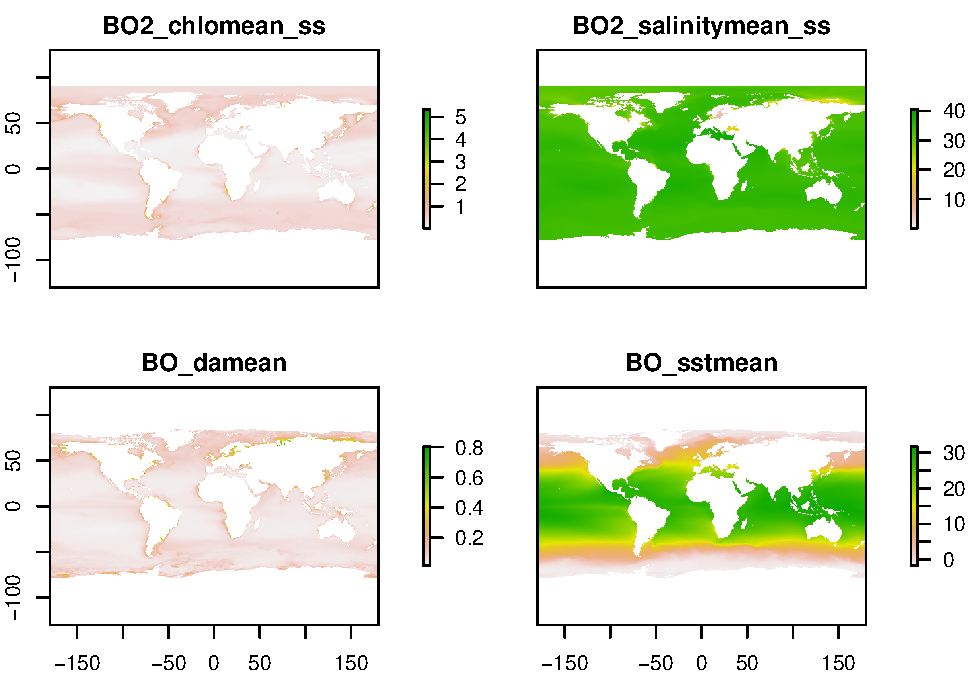
\includegraphics{_main_files/figure-latex/unnamed-chunk-33-1.pdf}

Note that the functions \texttt{dataset\_citations} and \texttt{layer\_citations} provide the bibliographic entries of the datasets and layers for proper citation:

\begin{Shaded}
\begin{Highlighting}[]
\FunctionTok{print}\NormalTok{(}\FunctionTok{dataset\_citations}\NormalTok{(}\StringTok{"Bio{-}ORACLE"}\NormalTok{))}
\end{Highlighting}
\end{Shaded}

\begin{verbatim}
## [1] "Assis J, Tyberghein L, Bosch S, Heroen V, Serrão E, De Clerck O, Tittensor D (2018). \"Bio‐ORACLE v2.0: Extending marine data layers for\nbioclimatic modelling.\" _Global Ecology and Biogeography_, *27*(3),\n277-284. doi:10.1111/geb.12693 <https://doi.org/10.1111/geb.12693>."                                 
## [2] "Tyberghein L, Heroen V, Pauly K, Troupin C, Mineur F, De Clerck O (2012). \"Bio-ORACLE: a global environmental dataset for marine species\ndistribution modelling.\" _Global Ecology and Biogeography_, *21*(2),\n272-281. doi:10.1111/j.1466-8238.2011.00656.x\n<https://doi.org/10.1111/j.1466-8238.2011.00656.x>."
\end{verbatim}

\begin{Shaded}
\begin{Highlighting}[]
\FunctionTok{print}\NormalTok{(}\FunctionTok{layer\_citations}\NormalTok{(}\StringTok{"BO2\_chlomean\_ss"}\NormalTok{))}
\end{Highlighting}
\end{Shaded}

\begin{verbatim}
## [1] "Assis J, Tyberghein L, Bosch S, Heroen V, Serrão E, De Clerck O, Tittensor D (2018). \"Bio‐ORACLE v2.0: Extending marine data layers for\nbioclimatic modelling.\" _Global Ecology and Biogeography_, *27*(3),\n277-284. doi:10.1111/geb.12693 <https://doi.org/10.1111/geb.12693>."                                 
## [2] "Tyberghein L, Heroen V, Pauly K, Troupin C, Mineur F, De Clerck O (2012). \"Bio-ORACLE: a global environmental dataset for marine species\ndistribution modelling.\" _Global Ecology and Biogeography_, *21*(2),\n272-281. doi:10.1111/j.1466-8238.2011.00656.x\n<https://doi.org/10.1111/j.1466-8238.2011.00656.x>."
\end{verbatim}

In case we are not interested on the whole area, we can crop the raster objects to the area of interest.

For example, we can load the \texttt{study\_area} object that is a SpatialPolygonsDataFrame that has been created previously and defines the extent of our spatial data and we can crop the rasterStack to the same extent:

\begin{Shaded}
\begin{Highlighting}[]
\FunctionTok{load}\NormalTok{(here}\SpecialCharTok{::}\FunctionTok{here}\NormalTok{ (}\StringTok{"data"}\NormalTok{, }\StringTok{"spatial"}\NormalTok{, }\StringTok{"study\_area.RData"}\NormalTok{))}

\NormalTok{mylayers }\OtherTok{\textless{}{-}} \FunctionTok{crop}\NormalTok{(myBioracle.layers, }\FunctionTok{extent}\NormalTok{(study\_area))}

\FunctionTok{plot}\NormalTok{(mylayers)}
\end{Highlighting}
\end{Shaded}

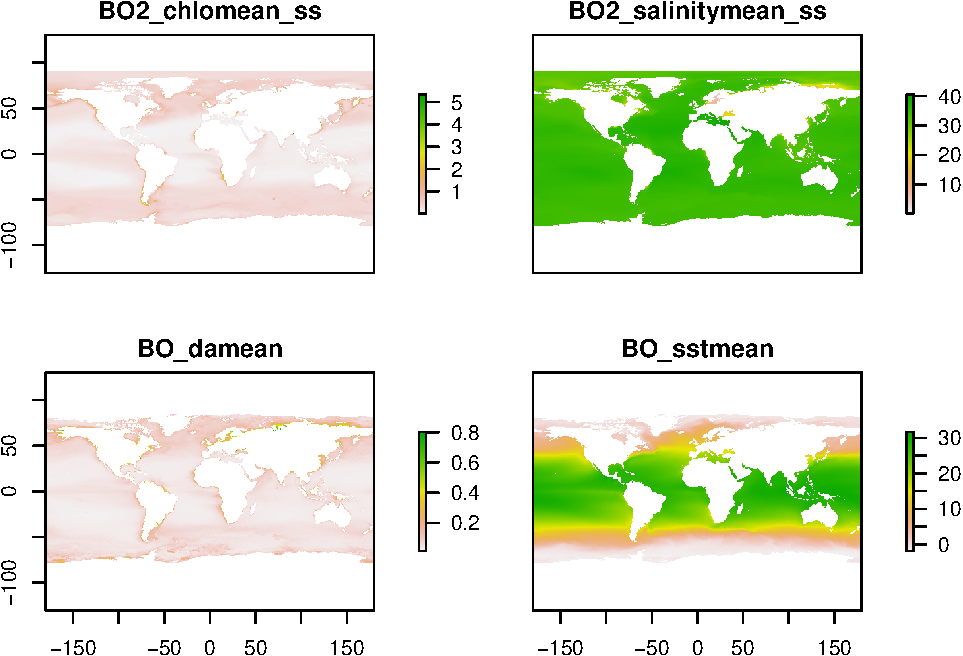
\includegraphics{_main_files/figure-latex/unnamed-chunk-35-1.pdf}

To facilitate subsequent access, the rasterStack with the downloaded data is saved in a local folder:

\begin{Shaded}
\begin{Highlighting}[]
\FunctionTok{writeRaster}\NormalTok{(mylayers, }\AttributeTok{filename=}\StringTok{"data/env/mylayers.tif"}\NormalTok{, }\AttributeTok{options=}\StringTok{"INTERLEAVE=BAND"}\NormalTok{, }\AttributeTok{overwrite=}\ConstantTok{TRUE}\NormalTok{)}
\end{Highlighting}
\end{Shaded}

\hypertarget{prepare-the-final-dataset}{%
\section{Prepare the final dataset}\label{prepare-the-final-dataset}}

In this chapter we first, extract environmental data associated to the presence-pseudoabsence data, we explore the data we got, we check correlation between variables and we calculate the Variance Inflation Factor (VIF) to make a selection of the variables we are going to use in the model.

First we load a list of required libraries.

\begin{Shaded}
\begin{Highlighting}[]
\NormalTok{requiredPackages }\OtherTok{\textless{}{-}} \FunctionTok{c}\NormalTok{(}
  \CommentTok{\#GENERAL USE LIBRARIES {-}{-}{-}{-}{-}{-}{-}{-}\#}
  \StringTok{"here"}\NormalTok{, }\CommentTok{\# Library for reproducible workflow}
  \StringTok{"rstudioapi"}\NormalTok{,  }\CommentTok{\# Library for reproducible workflow}
  
  \CommentTok{\#EXTRACT ENVIRONMENTAL DATA AND PLOTS}
  \StringTok{"sp"}\NormalTok{, }\CommentTok{\# spatial data}
  \StringTok{"raster"}\NormalTok{, }\CommentTok{\#spatial data}
  \StringTok{"dplyr"}\NormalTok{,}
  \StringTok{"tidyr"}\NormalTok{,}
  \StringTok{"ggplot2"}\NormalTok{,}
  \StringTok{"ggcorrplot"}\NormalTok{,}
  
  \CommentTok{\#CORRELATION ANALYSIS}
  \StringTok{"GGally"}\NormalTok{, }\CommentTok{\#correlation analysis}
  \StringTok{"HH"} \CommentTok{\#calculate VIF}
\NormalTok{    )}
\end{Highlighting}
\end{Shaded}

We run a function to install the required packages that are not in our system and load all the required packages.

\begin{Shaded}
\begin{Highlighting}[]
\NormalTok{install\_load\_function }\OtherTok{\textless{}{-}} \ControlFlowTok{function}\NormalTok{(pkg)\{}
\NormalTok{  new.pkg }\OtherTok{\textless{}{-}}\NormalTok{ pkg[}\SpecialCharTok{!}\NormalTok{(pkg }\SpecialCharTok{\%in\%} \FunctionTok{installed.packages}\NormalTok{()[, }\StringTok{"Package"}\NormalTok{])]}
  \ControlFlowTok{if}\NormalTok{ (}\FunctionTok{length}\NormalTok{(new.pkg))}
    \FunctionTok{install.packages}\NormalTok{(new.pkg, }\AttributeTok{dependencies =} \ConstantTok{TRUE}\NormalTok{)}
  \FunctionTok{sapply}\NormalTok{(pkg, require, }\AttributeTok{character.only =} \ConstantTok{TRUE}\NormalTok{)}
\NormalTok{\}}

\FunctionTok{install\_load\_function}\NormalTok{(requiredPackages)}
\end{Highlighting}
\end{Shaded}

\begin{verbatim}
##       here rstudioapi         sp     raster      dplyr      tidyr    ggplot2 
##       TRUE       TRUE       TRUE       TRUE       TRUE       TRUE       TRUE 
## ggcorrplot     GGally         HH 
##       TRUE       TRUE       TRUE
\end{verbatim}

We define some overall settings.

\begin{Shaded}
\begin{Highlighting}[]
\CommentTok{\# General settings for ggplot (black{-}white background, larger base\_size)}
\FunctionTok{theme\_set}\NormalTok{(}\FunctionTok{theme\_bw}\NormalTok{(}\AttributeTok{base\_size =} \DecValTok{16}\NormalTok{))}
\end{Highlighting}
\end{Shaded}

\hypertarget{extract-environmental-data-associated-to-presence-absence-data}{%
\section{Extract environmental data associated to presence-absence data}\label{extract-environmental-data-associated-to-presence-absence-data}}

Once we have prepared our species distribution data (occurrences and pseudo-absences) and the environmental rasters, we need to merge both sources of data. First, we load the objects created in previous sections:

\begin{Shaded}
\begin{Highlighting}[]
\CommentTok{\#load presence{-}absence data}
\FunctionTok{load}\NormalTok{(here}\SpecialCharTok{::}\FunctionTok{here}\NormalTok{ (}\StringTok{"data"}\NormalTok{, }\StringTok{"outputs\_for\_modelling"}\NormalTok{, }\StringTok{"PAdata.RData"}\NormalTok{))}

\CommentTok{\# load environmental rasters}
\NormalTok{mylayers}\OtherTok{\textless{}{-}}\FunctionTok{stack}\NormalTok{(here}\SpecialCharTok{::}\FunctionTok{here}\NormalTok{ (}\StringTok{"data"}\NormalTok{, }\StringTok{"env"}\NormalTok{, }\StringTok{"mylayers.tif"}\NormalTok{))}
\end{Highlighting}
\end{Shaded}

Now we can extract the environmental data associated to each of the species data points using the function \texttt{extract} from the \texttt{raster} package. The method employed is \texttt{bilinear} that returns the interpolated value from the four nearest raster cells.

\begin{Shaded}
\begin{Highlighting}[]
\NormalTok{raster\_ex }\OtherTok{\textless{}{-}}\NormalTok{ raster}\SpecialCharTok{::}\FunctionTok{extract}\NormalTok{(}\AttributeTok{x=}\NormalTok{mylayers, }\AttributeTok{y=}\NormalTok{PAdata[,}\FunctionTok{c}\NormalTok{(}\StringTok{"LON"}\NormalTok{,}\StringTok{"LAT"}\NormalTok{)], }\AttributeTok{method=}\StringTok{"bilinear"}\NormalTok{, }\AttributeTok{na.rm=}\ConstantTok{TRUE}\NormalTok{, }\AttributeTok{df=}\NormalTok{T) }

\FunctionTok{colnames}\NormalTok{(raster\_ex)[}\SpecialCharTok{{-}}\DecValTok{1}\NormalTok{]}\OtherTok{\textless{}{-}}\FunctionTok{c}\NormalTok{(}\StringTok{"BO2\_chlomean\_ss"}\NormalTok{, }\StringTok{"BO2\_salinitymean\_ss"}\NormalTok{, }\StringTok{"BO\_damean"}\NormalTok{ ,}\StringTok{"BO\_sstmean"}\NormalTok{)}

\FunctionTok{head}\NormalTok{(raster\_ex)}
\end{Highlighting}
\end{Shaded}

\begin{verbatim}
##   ID BO2_chlomean_ss BO2_salinitymean_ss BO_damean BO_sstmean
## 1  1      1.20410309            35.42666 0.1973854   16.99439
## 2  2      1.20410309            35.42666 0.1973854   16.99439
## 3  3      0.08455528            36.43070 0.0290000   25.52963
## 4  4      1.20410309            35.42666 0.1973854   16.99439
## 5  5      0.72283228            34.20426 0.0817736   15.21486
## 6  6      1.20410309            35.42666 0.1973854   16.99439
\end{verbatim}

We merge the presence/absence data and the environmental data:

\begin{Shaded}
\begin{Highlighting}[]
\NormalTok{data }\OtherTok{\textless{}{-}} \FunctionTok{cbind}\NormalTok{(PAdata, raster\_ex)}
\end{Highlighting}
\end{Shaded}

We can conduct some quick checks on the new dataset:

\begin{Shaded}
\begin{Highlighting}[]
\FunctionTok{dim}\NormalTok{(data)}
\end{Highlighting}
\end{Shaded}

\begin{verbatim}
## [1] 29806    10
\end{verbatim}

\begin{Shaded}
\begin{Highlighting}[]
\FunctionTok{str}\NormalTok{(data)}
\end{Highlighting}
\end{Shaded}

\begin{verbatim}
## 'data.frame':    29806 obs. of  10 variables:
##  $ scientificName     : chr  "Thunnus alalunga" "Thunnus alalunga" "Thunnus alalunga" "Thunnus alalunga" ...
##  $ LON                : num  18.5 18.5 -76.6 18.5 -69.3 ...
##  $ LAT                : num  -34.4 -34.4 28.4 -34.4 39.9 ...
##  $ YEAR               : num  2004 2004 2000 2000 2000 ...
##  $ occurrenceStatus   : num  1 1 1 1 1 1 1 1 1 1 ...
##  $ ID                 : num  1 2 3 4 5 6 7 8 9 10 ...
##  $ BO2_chlomean_ss    : num  1.2041 1.2041 0.0846 1.2041 0.7228 ...
##  $ BO2_salinitymean_ss: num  35.4 35.4 36.4 35.4 34.2 ...
##  $ BO_damean          : num  0.1974 0.1974 0.029 0.1974 0.0818 ...
##  $ BO_sstmean         : num  17 17 25.5 17 15.2 ...
\end{verbatim}

\begin{Shaded}
\begin{Highlighting}[]
\FunctionTok{head}\NormalTok{(data)}
\end{Highlighting}
\end{Shaded}

\begin{verbatim}
##      scientificName      LON      LAT YEAR occurrenceStatus ID BO2_chlomean_ss
## 1  Thunnus alalunga  18.4972 -34.3569 2004                1  1      1.20410309
## 5  Thunnus alalunga  18.4972 -34.3569 2004                1  2      1.20410309
## 8  Thunnus alalunga -76.6000  28.4000 2000                1  3      0.08455528
## 10 Thunnus alalunga  18.4972 -34.3569 2000                1  4      1.20410309
## 11 Thunnus alalunga -69.3100  39.8800 2000                1  5      0.72283228
## 12 Thunnus alalunga  18.4972 -34.3569 2001                1  6      1.20410309
##    BO2_salinitymean_ss BO_damean BO_sstmean
## 1             35.42666 0.1973854   16.99439
## 5             35.42666 0.1973854   16.99439
## 8             36.43070 0.0290000   25.52963
## 10            35.42666 0.1973854   16.99439
## 11            34.20426 0.0817736   15.21486
## 12            35.42666 0.1973854   16.99439
\end{verbatim}

\begin{Shaded}
\begin{Highlighting}[]
\FunctionTok{summary}\NormalTok{(data)}
\end{Highlighting}
\end{Shaded}

\begin{verbatim}
##  scientificName          LON               LAT               YEAR      
##  Length:29806       Min.   :-97.805   Min.   :-82.187   Min.   :2000   
##  Class :character   1st Qu.:-69.221   1st Qu.:-29.933   1st Qu.:2001   
##  Mode  :character   Median :-28.967   Median : 24.006   Median :2002   
##                     Mean   :-31.118   Mean   :  7.678   Mean   :2003   
##                     3rd Qu.:  2.933   3rd Qu.: 38.250   3rd Qu.:2004   
##                     Max.   : 67.648   Max.   : 89.418   Max.   :2013   
##                                                         NA's   :14903  
##  occurrenceStatus       ID        BO2_chlomean_ss   BO2_salinitymean_ss
##  Min.   :0.0      Min.   :    1   Min.   :0.01585   Min.   : 0.1632    
##  1st Qu.:0.0      1st Qu.: 7452   1st Qu.:0.08960   1st Qu.:34.5032    
##  Median :0.5      Median :14904   Median :0.24648   Median :35.4267    
##  Mean   :0.5      Mean   :14904   Mean   :0.42505   Mean   :35.2388    
##  3rd Qu.:1.0      3rd Qu.:22355   3rd Qu.:0.68378   3rd Qu.:36.2156    
##  Max.   :1.0      Max.   :29806   Max.   :3.44767   Max.   :39.2467    
##                                   NA's   :98        NA's   :98         
##    BO_damean         BO_sstmean    
##  Min.   :0.02180   Min.   :-1.705  
##  1st Qu.:0.03505   1st Qu.:14.852  
##  Median :0.05039   Median :18.898  
##  Mean   :0.07833   Mean   :18.117  
##  3rd Qu.:0.08800   3rd Qu.:25.373  
##  Max.   :0.69655   Max.   :30.663  
##  NA's   :139       NA's   :139
\end{verbatim}

The new dataset has 29806 rows and 10 columns, and there are 139 NA's in the environmental dataset. We remove the points with NA's:

\begin{Shaded}
\begin{Highlighting}[]
\NormalTok{data }\OtherTok{\textless{}{-}}\NormalTok{ data }\SpecialCharTok{\%\textgreater{}\%} 
\NormalTok{  dplyr}\SpecialCharTok{::}\FunctionTok{select}\NormalTok{ (}\SpecialCharTok{{-}}\NormalTok{YEAR) }\SpecialCharTok{\%\textgreater{}\%} \CommentTok{\#we remove year column because pseudoabsences miss this info}
  \FunctionTok{na.omit}\NormalTok{()}
\end{Highlighting}
\end{Shaded}

We check again the dataset:

\begin{Shaded}
\begin{Highlighting}[]
\FunctionTok{dim}\NormalTok{(data)}
\end{Highlighting}
\end{Shaded}

\begin{verbatim}
## [1] 29661     9
\end{verbatim}

\begin{Shaded}
\begin{Highlighting}[]
\FunctionTok{summary}\NormalTok{(data) }
\end{Highlighting}
\end{Shaded}

\begin{verbatim}
##  scientificName          LON               LAT          occurrenceStatus
##  Length:29661       Min.   :-97.805   Min.   :-77.508   Min.   :0.0000  
##  Class :character   1st Qu.:-69.330   1st Qu.:-29.933   1st Qu.:0.0000  
##  Mode  :character   Median :-28.946   Median : 24.088   Median :1.0000  
##                     Mean   :-31.138   Mean   :  7.792   Mean   :0.5024  
##                     3rd Qu.:  2.938   3rd Qu.: 38.242   3rd Qu.:1.0000  
##                     Max.   : 67.241   Max.   : 83.660   Max.   :1.0000  
##        ID        BO2_chlomean_ss   BO2_salinitymean_ss   BO_damean      
##  Min.   :    1   Min.   :0.01585   Min.   : 0.1632     Min.   :0.02180  
##  1st Qu.: 7416   1st Qu.:0.08954   1st Qu.:34.5100     1st Qu.:0.03504  
##  Median :14831   Median :0.24526   Median :35.4267     Median :0.05037  
##  Mean   :14865   Mean   :0.42527   Mean   :35.2420     Mean   :0.07833  
##  3rd Qu.:22313   3rd Qu.:0.68457   3rd Qu.:36.2163     3rd Qu.:0.08800  
##  Max.   :29806   Max.   :3.44767   Max.   :39.2467     Max.   :0.69655  
##    BO_sstmean    
##  Min.   :-1.705  
##  1st Qu.:14.853  
##  Median :18.899  
##  Mean   :18.120  
##  3rd Qu.:25.374  
##  Max.   :30.663
\end{verbatim}

The resulting dataset has 29661. We save this dataset in a local file to work on it in subsequent steps.

\begin{Shaded}
\begin{Highlighting}[]
\FunctionTok{save}\NormalTok{(}\AttributeTok{list=}\StringTok{"data"}\NormalTok{, }\AttributeTok{file=}\StringTok{"data/outputs\_for\_modelling/PAdata\_with\_env.RData"}\NormalTok{)}
\end{Highlighting}
\end{Shaded}

\hypertarget{exploratory-plots-of-environmental-variables}{%
\section{Exploratory plots of environmental variables}\label{exploratory-plots-of-environmental-variables}}

Before starting the modelling process, we are going to explore the individual variables in the dataset.

We can explore the distributions of each of the environmental variables by looking at the violin and boxplots and at the histograms and density plots as follows:

\begin{Shaded}
\begin{Highlighting}[]
\NormalTok{tmp }\OtherTok{\textless{}{-}}\NormalTok{ data[, }\FunctionTok{c}\NormalTok{(}\StringTok{"BO2\_chlomean\_ss"}\NormalTok{,}\StringTok{"BO2\_salinitymean\_ss"}\NormalTok{,}\StringTok{"BO\_damean"}\NormalTok{,}\StringTok{"BO\_sstmean"}\NormalTok{)]}
\NormalTok{tmp }\OtherTok{\textless{}{-}} \FunctionTok{pivot\_longer}\NormalTok{(}\AttributeTok{data=}\NormalTok{tmp, }\AttributeTok{cols=}\FunctionTok{everything}\NormalTok{()) }

\FunctionTok{ggplot}\NormalTok{(}\AttributeTok{data=}\NormalTok{tmp, }\FunctionTok{aes}\NormalTok{(}\AttributeTok{x=}\NormalTok{name, }\AttributeTok{y=}\NormalTok{value)) }\SpecialCharTok{+} 
  \FunctionTok{geom\_boxplot}\NormalTok{()}\SpecialCharTok{+}
  \FunctionTok{facet\_wrap}\NormalTok{(}\SpecialCharTok{\textasciitilde{}}\NormalTok{name, }\AttributeTok{scales=}\StringTok{"free"}\NormalTok{)}
\end{Highlighting}
\end{Shaded}

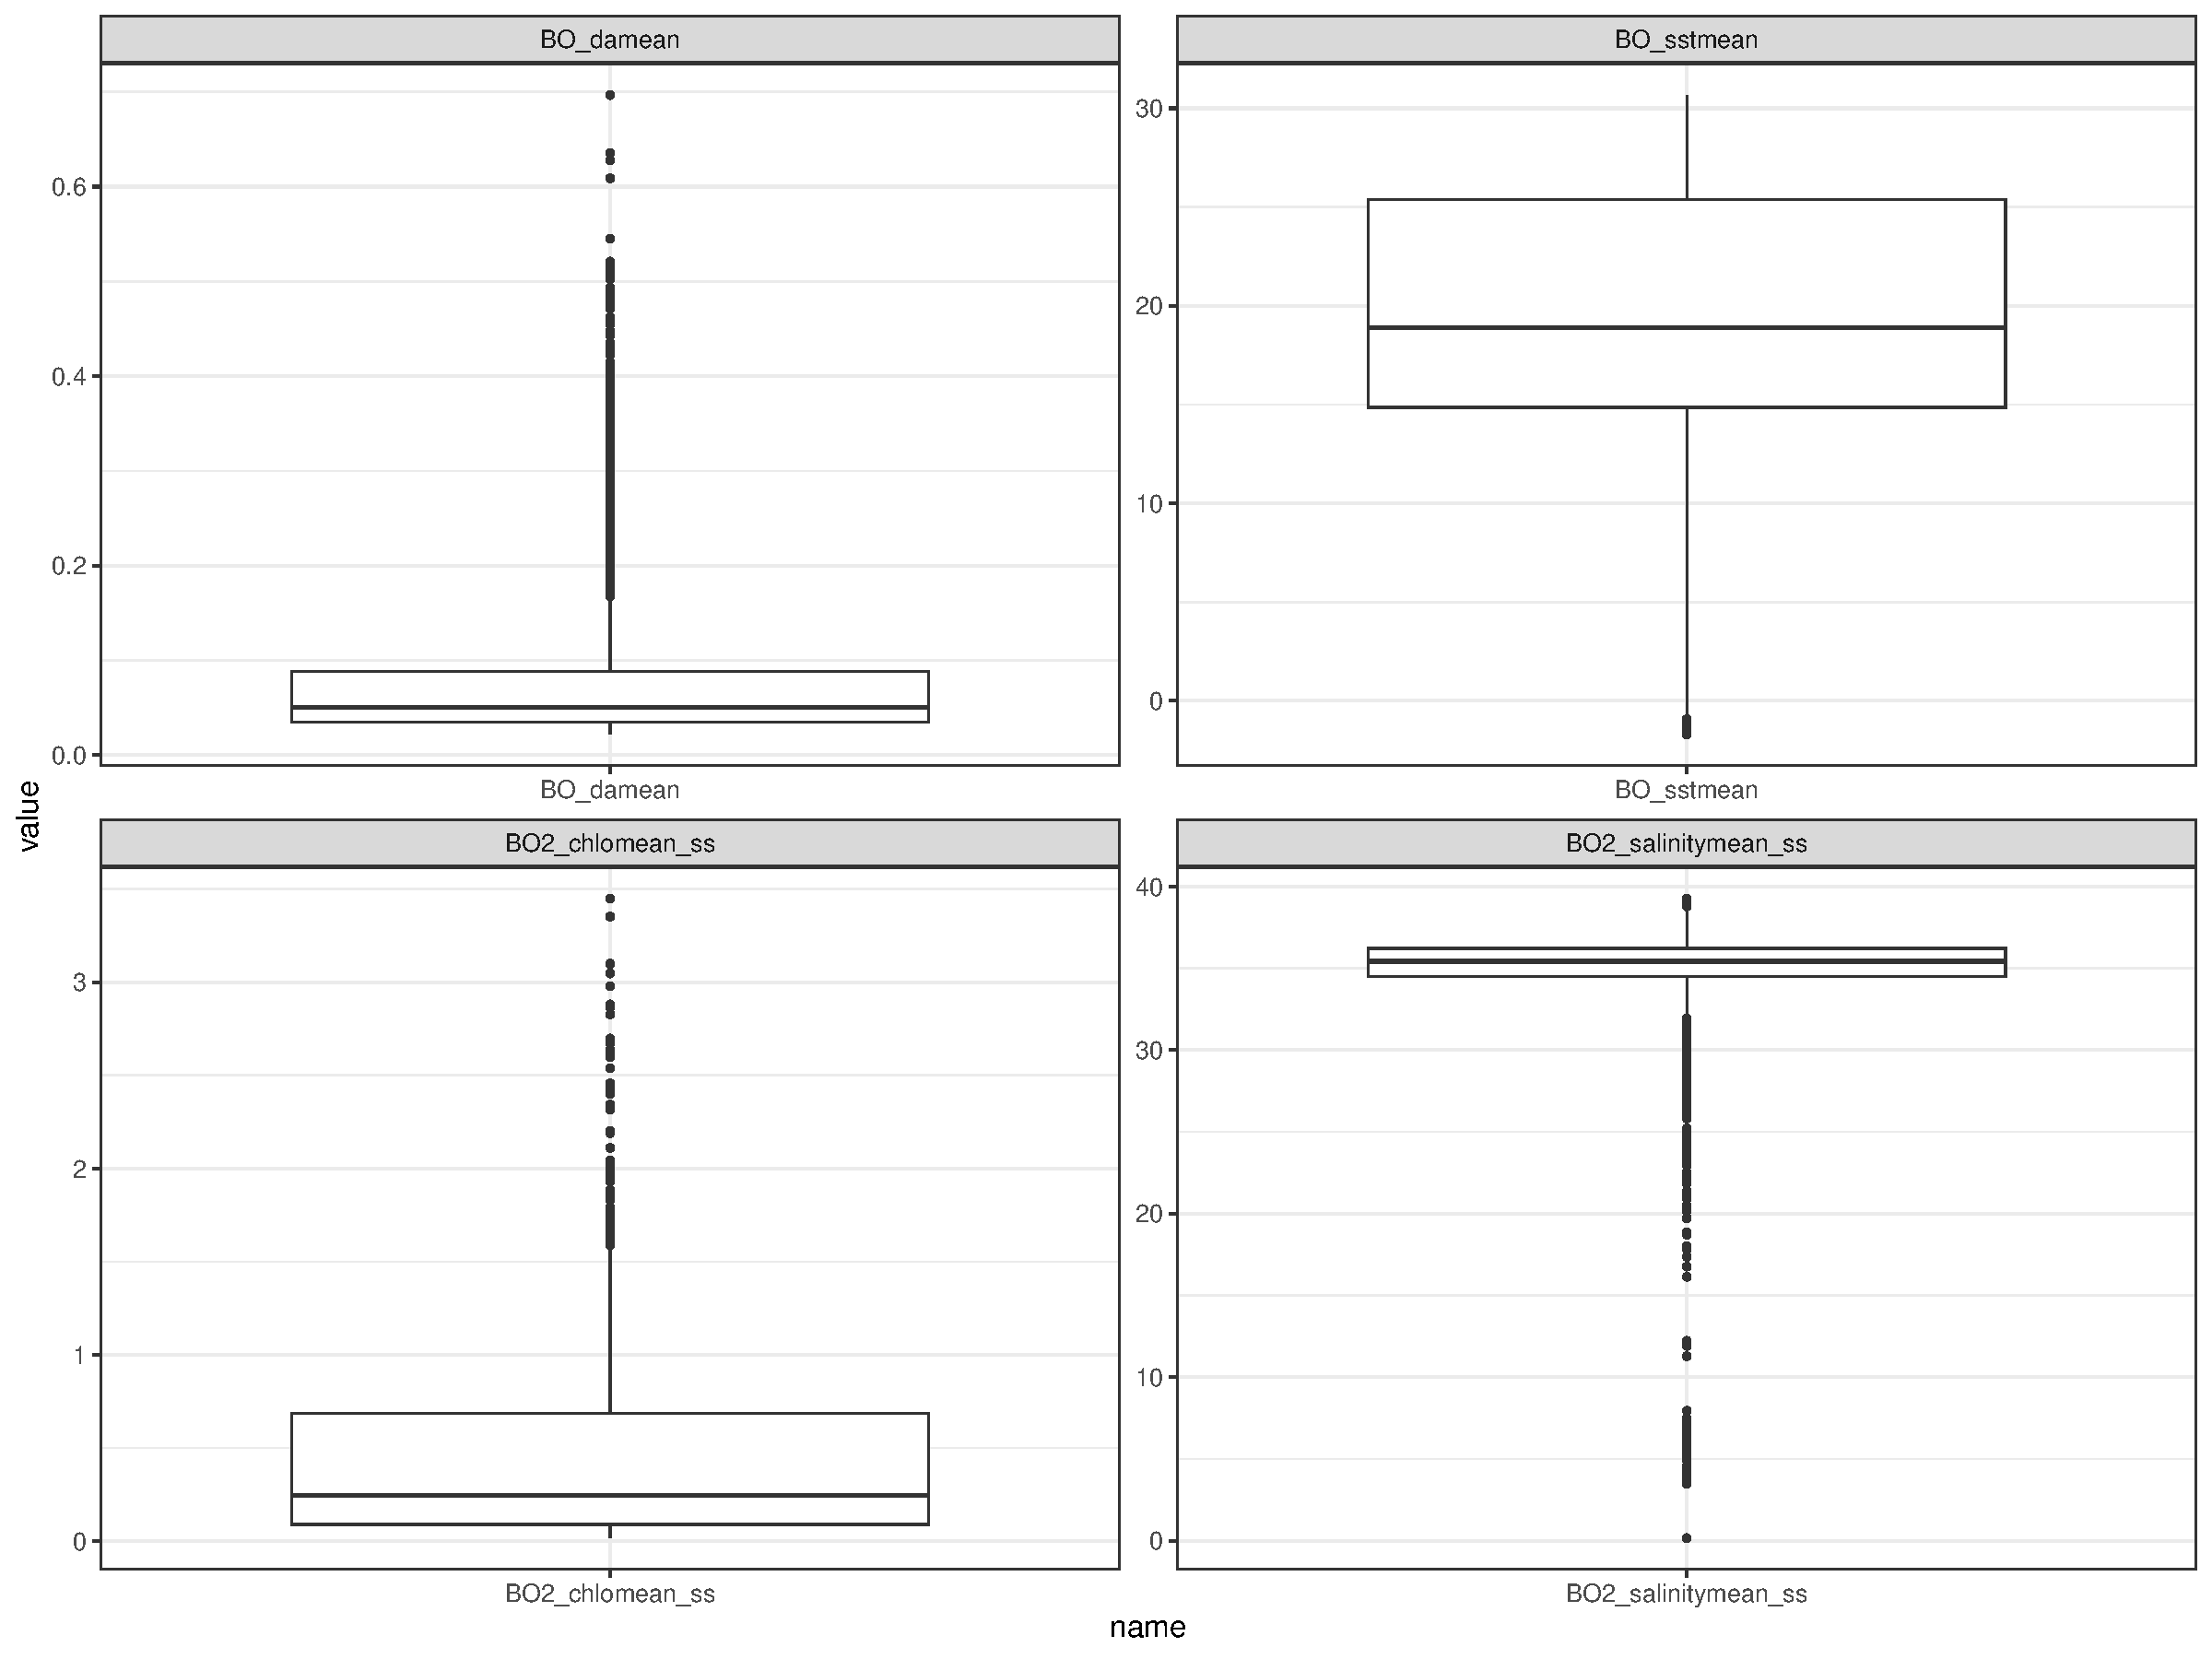
\includegraphics{_main_files/figure-latex/unnamed-chunk-47-1.pdf}

\begin{Shaded}
\begin{Highlighting}[]
\FunctionTok{ggplot}\NormalTok{(}\AttributeTok{data=}\NormalTok{tmp, }\FunctionTok{aes}\NormalTok{(}\AttributeTok{x=}\NormalTok{name, }\AttributeTok{y=}\NormalTok{value)) }\SpecialCharTok{+} 
  \FunctionTok{geom\_violin}\NormalTok{(}\AttributeTok{fill=}\StringTok{"red"}\NormalTok{, }\AttributeTok{alpha=}\FloatTok{0.3}\NormalTok{)}\SpecialCharTok{+}
  \FunctionTok{geom\_boxplot}\NormalTok{(}\AttributeTok{width=}\FloatTok{0.1}\NormalTok{)}\SpecialCharTok{+}
  \FunctionTok{facet\_wrap}\NormalTok{(}\SpecialCharTok{\textasciitilde{}}\NormalTok{name, }\AttributeTok{scales=}\StringTok{"free"}\NormalTok{)}
\end{Highlighting}
\end{Shaded}

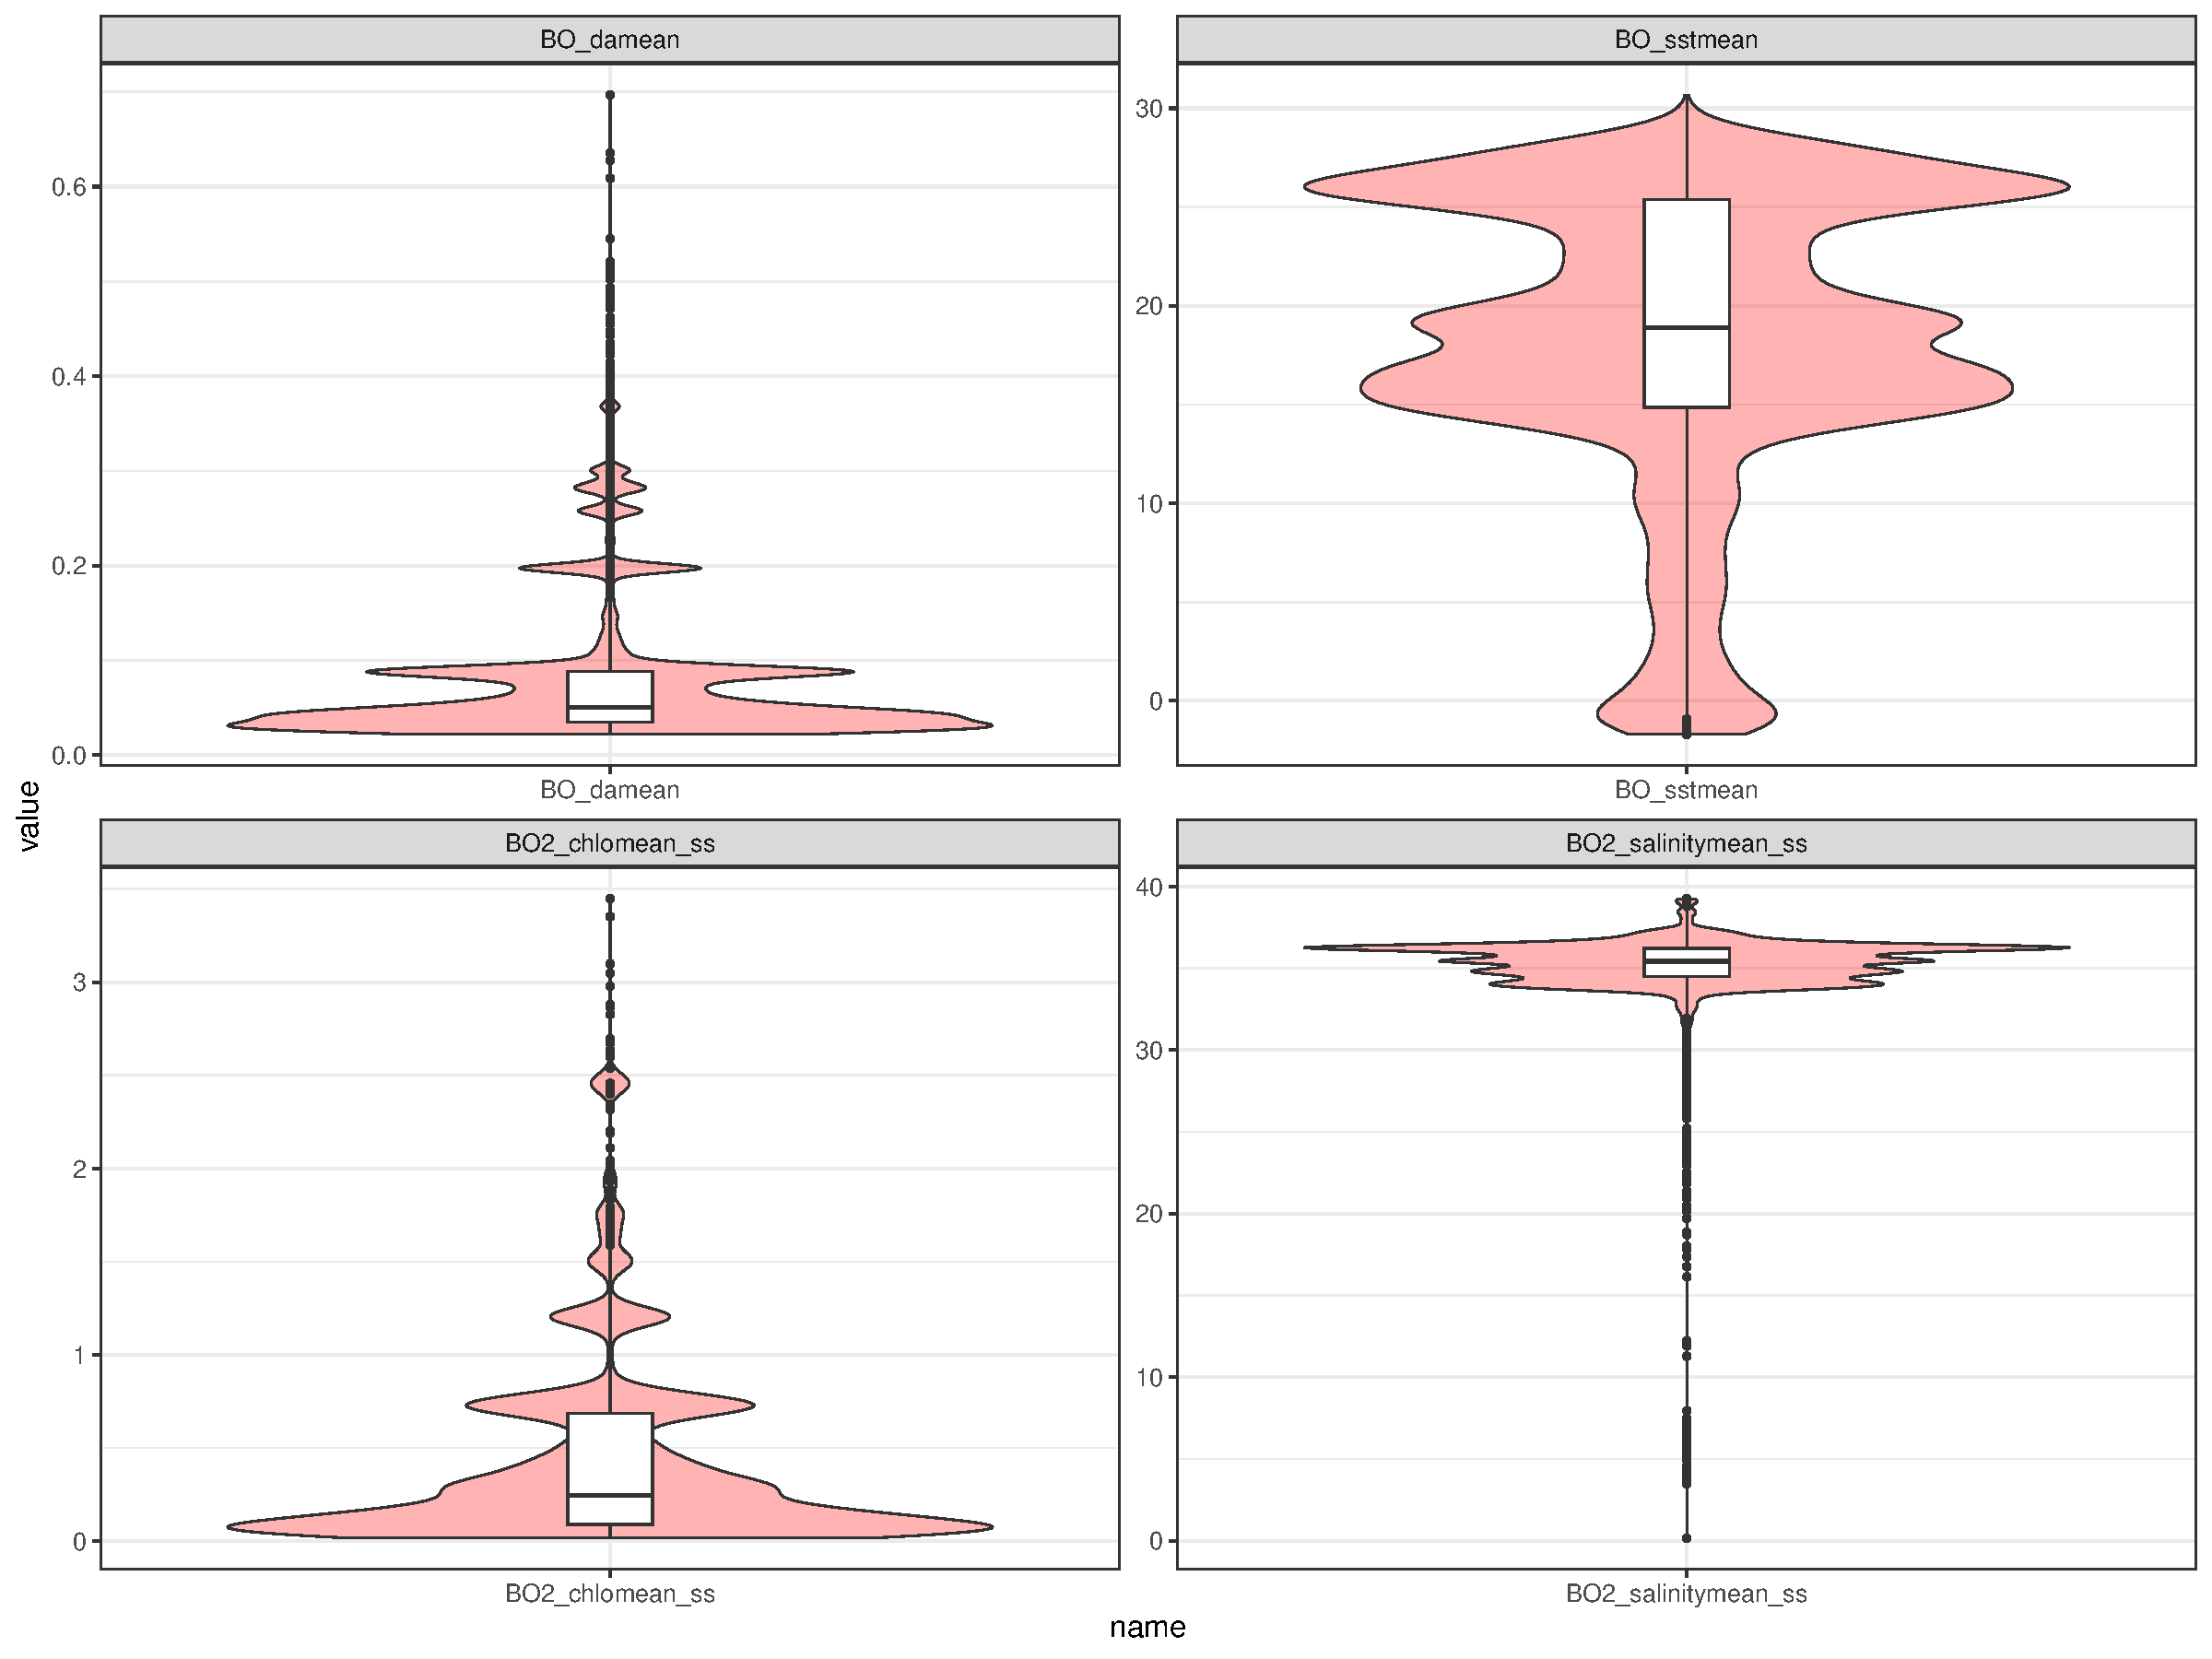
\includegraphics{_main_files/figure-latex/unnamed-chunk-47-2.pdf}

\begin{Shaded}
\begin{Highlighting}[]
\FunctionTok{ggplot}\NormalTok{(}\AttributeTok{data=}\NormalTok{tmp, }\FunctionTok{aes}\NormalTok{(}\AttributeTok{x=}\NormalTok{value)) }\SpecialCharTok{+} 
  \FunctionTok{geom\_histogram}\NormalTok{(}\FunctionTok{aes}\NormalTok{(}\AttributeTok{y=} \FunctionTok{after\_stat}\NormalTok{(density)), }\AttributeTok{colour=}\DecValTok{1}\NormalTok{, }\AttributeTok{fill=}\StringTok{"red"}\NormalTok{, }\AttributeTok{alpha=}\FloatTok{0.3}\NormalTok{)}\SpecialCharTok{+}
  \FunctionTok{geom\_density}\NormalTok{(}\AttributeTok{lwd=}\DecValTok{1}\NormalTok{)}\SpecialCharTok{+}
  \FunctionTok{facet\_wrap}\NormalTok{(}\SpecialCharTok{\textasciitilde{}}\NormalTok{name, }\AttributeTok{scales=}\StringTok{"free"}\NormalTok{)}
\end{Highlighting}
\end{Shaded}

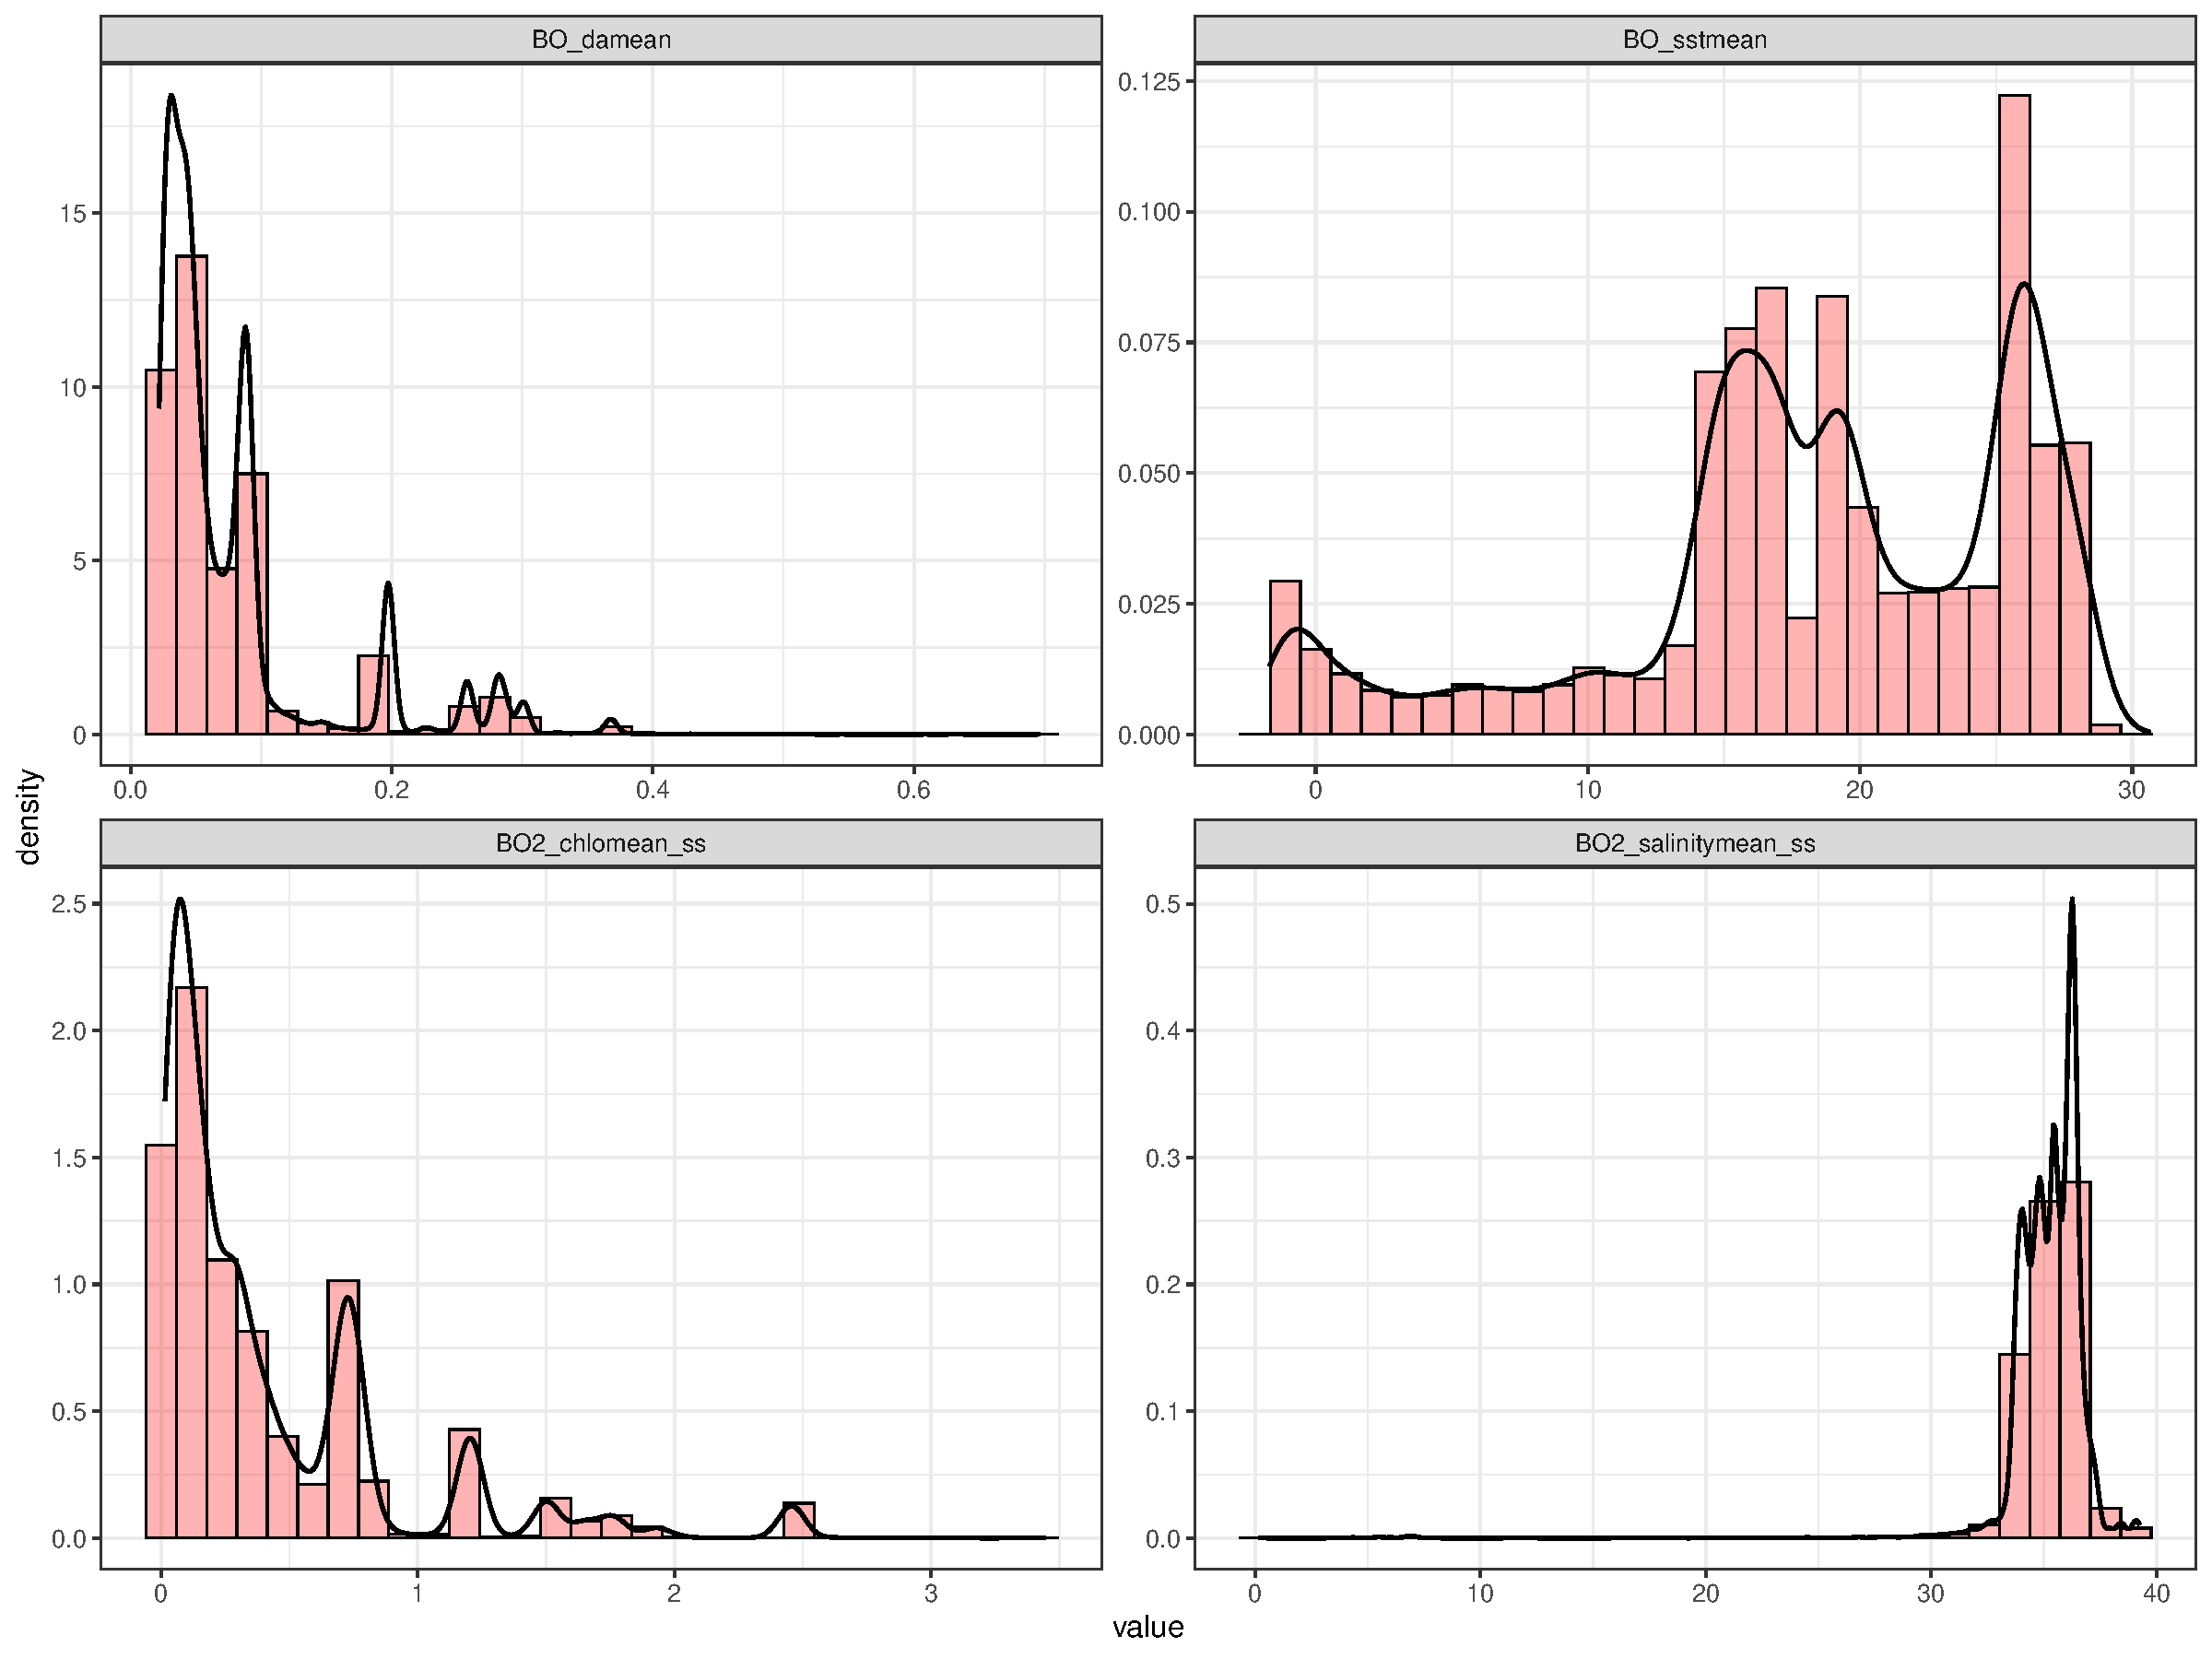
\includegraphics{_main_files/figure-latex/unnamed-chunk-47-3.pdf}

\hypertarget{exploratory-plots-of-environmental-variables-depending-on-presenceabsence-data}{%
\section{Exploratory plots of environmental variables depending on presence/absence data}\label{exploratory-plots-of-environmental-variables-depending-on-presenceabsence-data}}

To analyse if there are preferences for certain ranges of the environmental variables, we compare the distribution of the environmental variables for presence and absence data:

\begin{Shaded}
\begin{Highlighting}[]
\NormalTok{tmp }\OtherTok{\textless{}{-}}\NormalTok{ data[, }\FunctionTok{c}\NormalTok{(}\StringTok{"LON"}\NormalTok{, }\StringTok{"LAT"}\NormalTok{, }\StringTok{"BO2\_chlomean\_ss"}\NormalTok{,}\StringTok{"BO2\_salinitymean\_ss"}\NormalTok{,}\StringTok{"BO\_damean"}\NormalTok{,}\StringTok{"BO\_sstmean"}\NormalTok{,}\StringTok{"occurrenceStatus"}\NormalTok{)]}
\NormalTok{tmp }\OtherTok{\textless{}{-}} \FunctionTok{pivot\_longer}\NormalTok{(}\AttributeTok{data=}\NormalTok{tmp, }\AttributeTok{cols=}\SpecialCharTok{!}\NormalTok{occurrenceStatus) }

\FunctionTok{ggplot}\NormalTok{(}\AttributeTok{data=}\NormalTok{tmp, }\FunctionTok{aes}\NormalTok{(}\AttributeTok{x=}\FunctionTok{factor}\NormalTok{(occurrenceStatus), }\AttributeTok{y=}\NormalTok{value, }\AttributeTok{fill=}\FunctionTok{factor}\NormalTok{(occurrenceStatus), }\AttributeTok{group=}\FunctionTok{factor}\NormalTok{(occurrenceStatus))) }\SpecialCharTok{+} 
  \FunctionTok{geom\_violin}\NormalTok{(}\AttributeTok{alpha=}\FloatTok{0.3}\NormalTok{)}\SpecialCharTok{+}
  \FunctionTok{geom\_boxplot}\NormalTok{(}\AttributeTok{fill=}\StringTok{"white"}\NormalTok{, }\AttributeTok{width=}\FloatTok{0.1}\NormalTok{)}\SpecialCharTok{+}
  \FunctionTok{facet\_wrap}\NormalTok{(}\SpecialCharTok{\textasciitilde{}}\NormalTok{name, }\AttributeTok{scales=}\StringTok{"free"}\NormalTok{)}\SpecialCharTok{+}
  \FunctionTok{theme}\NormalTok{(}\AttributeTok{legend.position =} \StringTok{"bottom"}\NormalTok{,}\AttributeTok{legend.background =} \FunctionTok{element\_rect}\NormalTok{(}\AttributeTok{fill =} \StringTok{"white"}\NormalTok{, }\AttributeTok{colour =} \ConstantTok{NA}\NormalTok{))}
\end{Highlighting}
\end{Shaded}

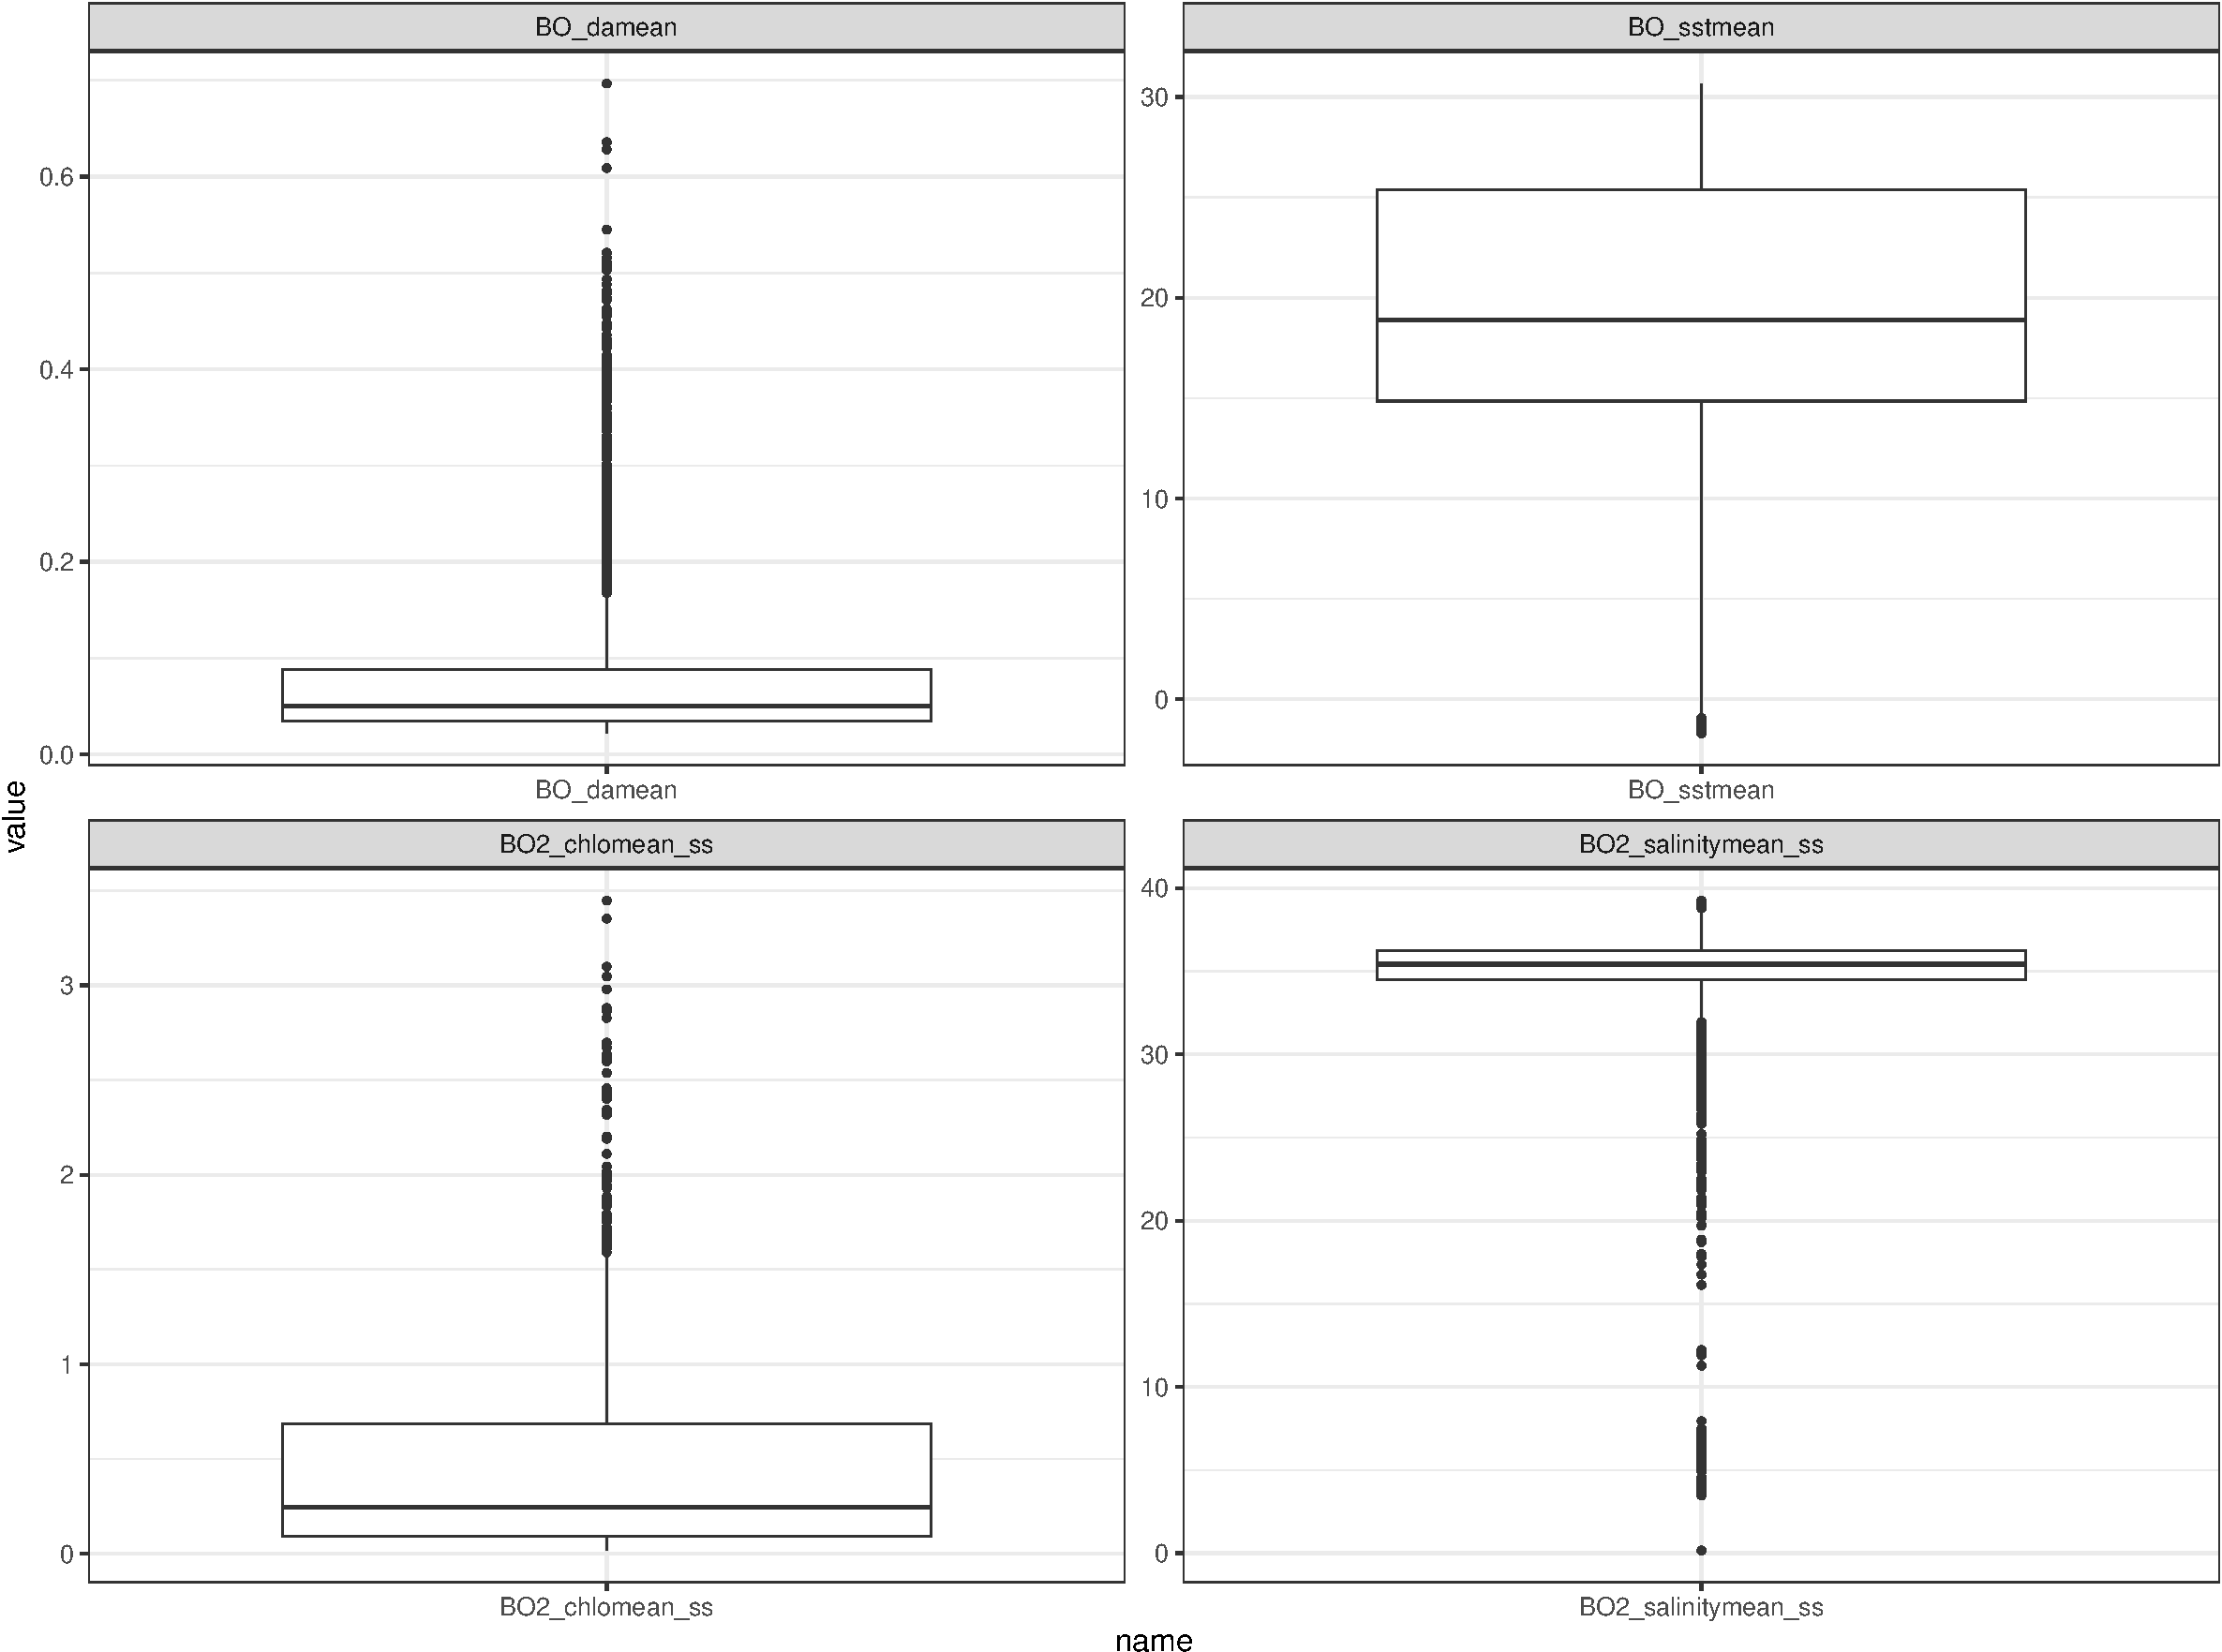
\includegraphics{_main_files/figure-latex/unnamed-chunk-48-1.pdf}

\begin{Shaded}
\begin{Highlighting}[]
\FunctionTok{ggplot}\NormalTok{(}\AttributeTok{data=}\NormalTok{tmp, }\FunctionTok{aes}\NormalTok{(}\AttributeTok{x=}\NormalTok{value, }\AttributeTok{fill=}\FunctionTok{factor}\NormalTok{(occurrenceStatus), }\AttributeTok{group=}\FunctionTok{factor}\NormalTok{(occurrenceStatus))) }\SpecialCharTok{+} 
  \FunctionTok{geom\_density}\NormalTok{(}\AttributeTok{lwd=}\DecValTok{1}\NormalTok{, }\AttributeTok{alpha=}\FloatTok{0.3}\NormalTok{)}\SpecialCharTok{+}
  \FunctionTok{facet\_wrap}\NormalTok{(}\SpecialCharTok{\textasciitilde{}}\NormalTok{name, }\AttributeTok{scales=}\StringTok{"free"}\NormalTok{)}\SpecialCharTok{+}
  \FunctionTok{theme}\NormalTok{(}\AttributeTok{legend.position =} \StringTok{"bottom"}\NormalTok{,}\AttributeTok{legend.background =} \FunctionTok{element\_rect}\NormalTok{(}\AttributeTok{fill =} \StringTok{"white"}\NormalTok{, }\AttributeTok{colour =} \ConstantTok{NA}\NormalTok{))}
\end{Highlighting}
\end{Shaded}

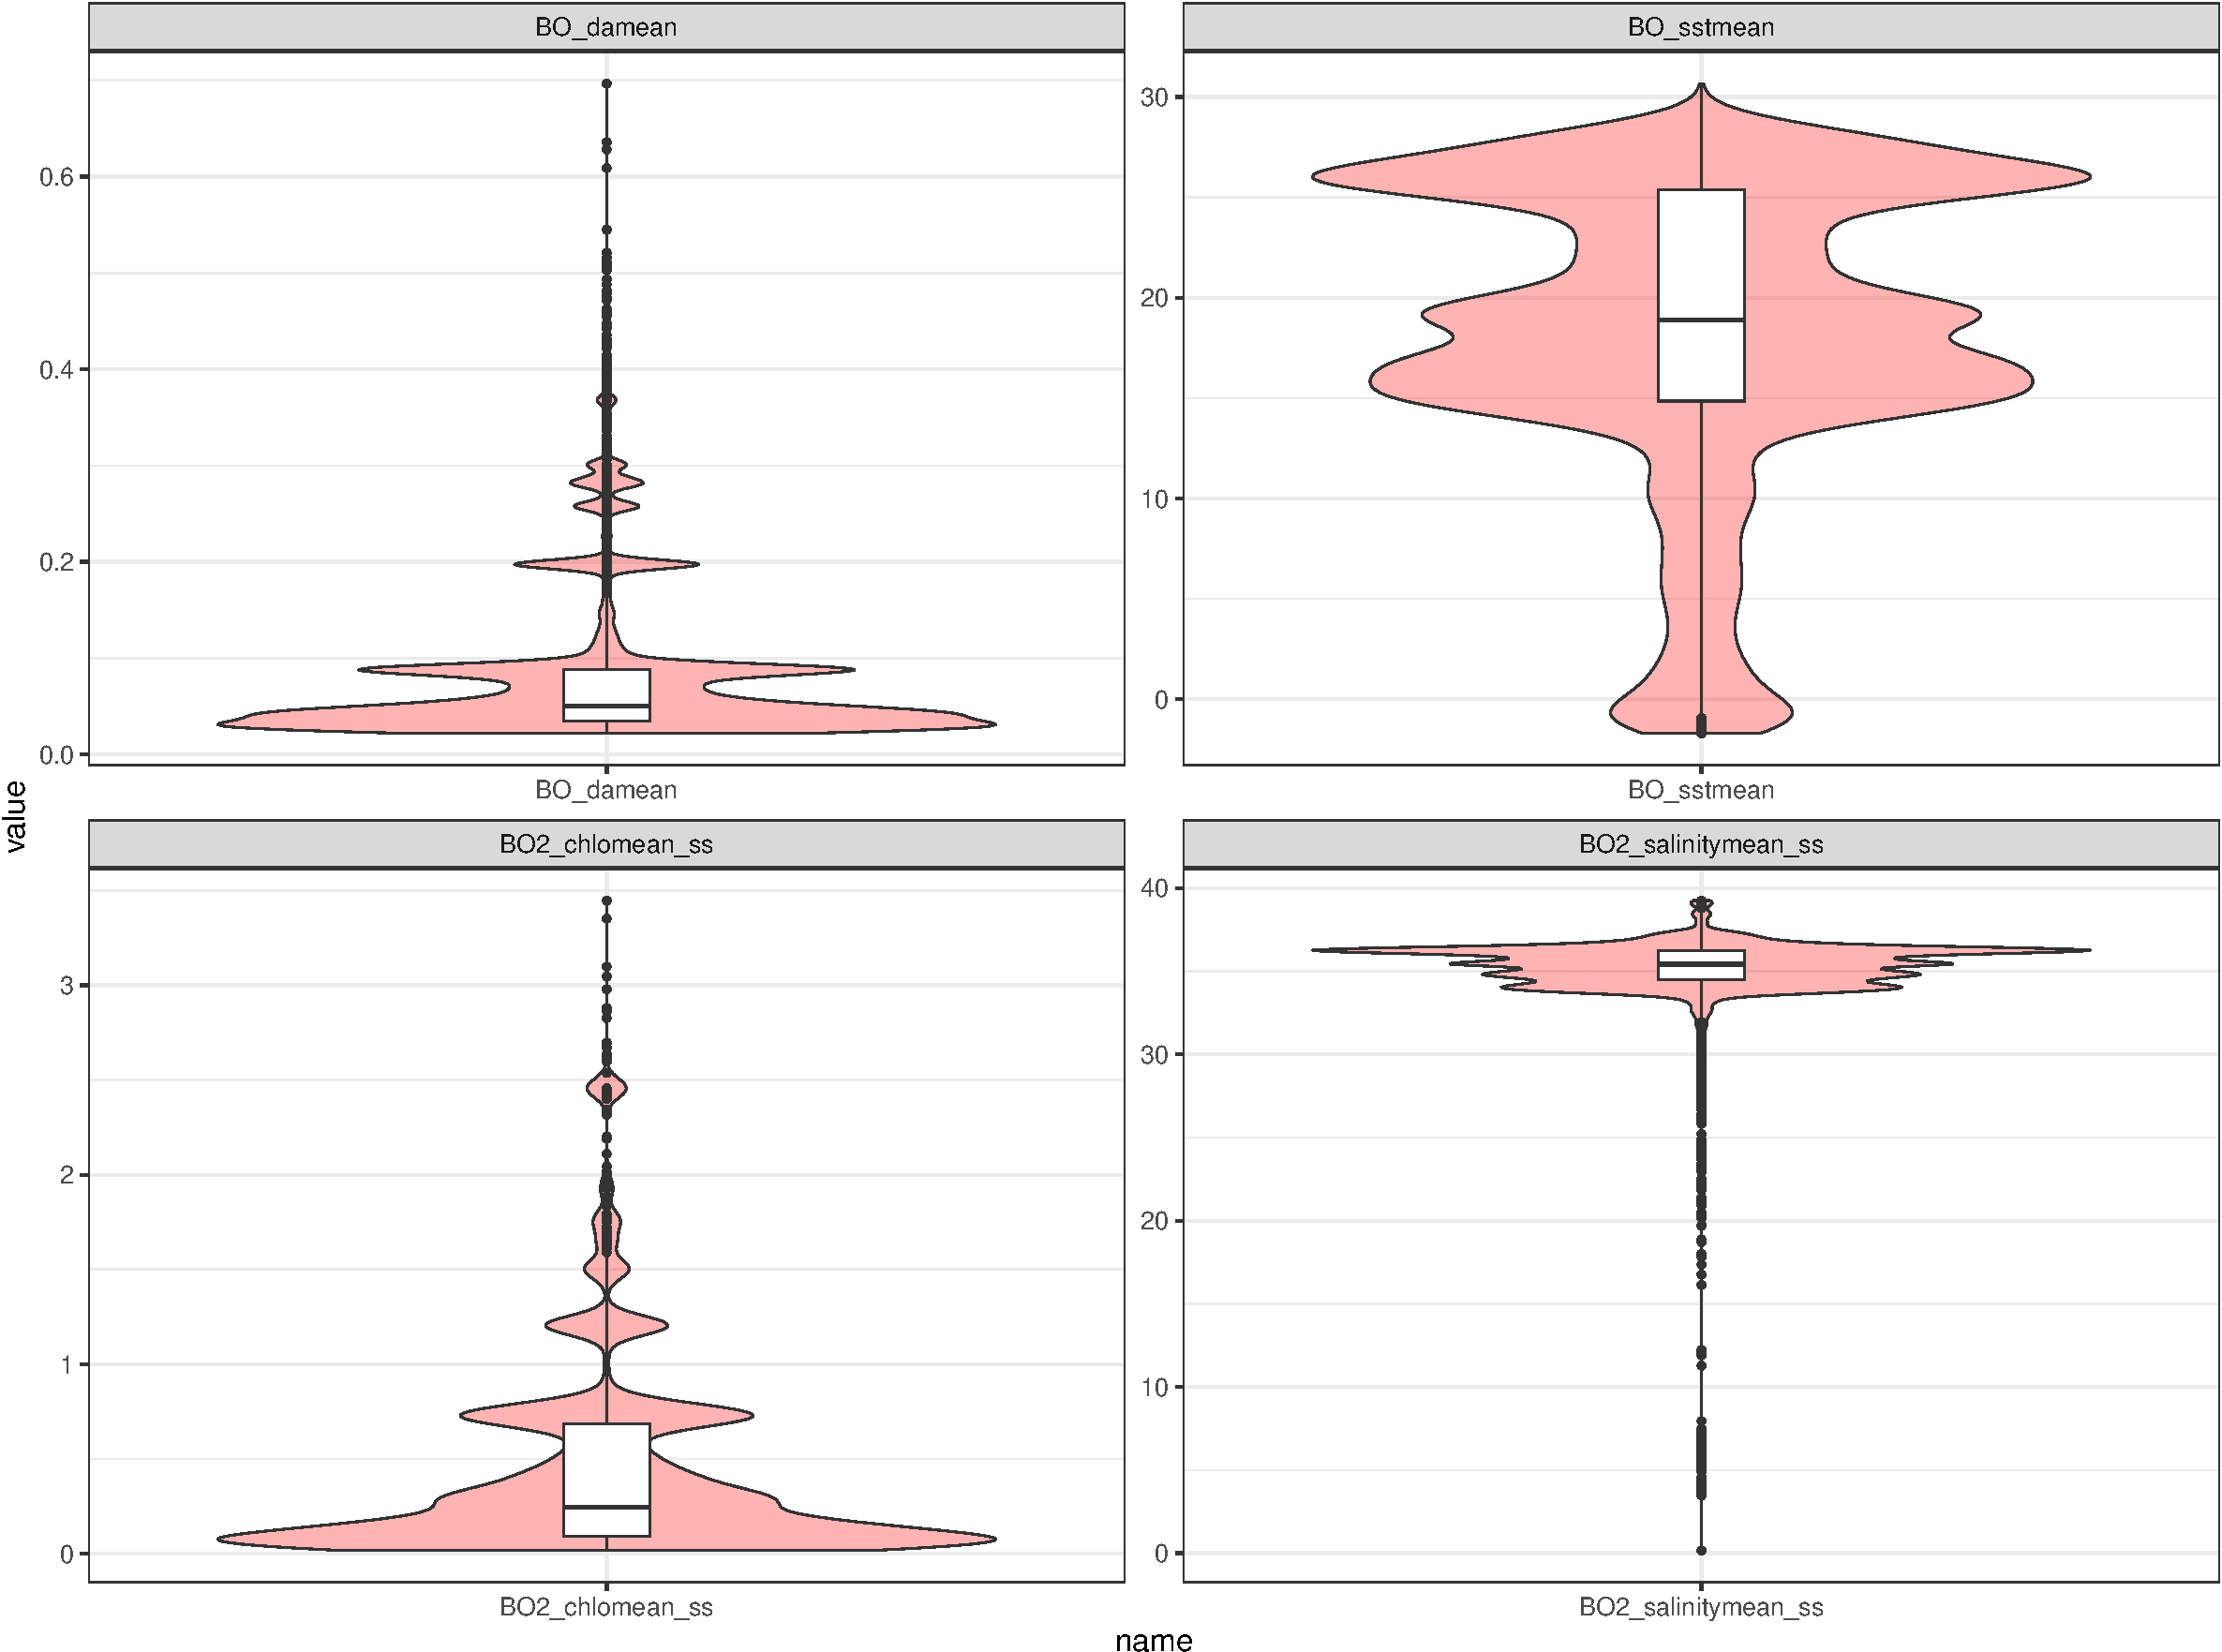
\includegraphics{_main_files/figure-latex/unnamed-chunk-48-2.pdf}

\hypertarget{correlation-analysis}{%
\section{Correlation analysis}\label{correlation-analysis}}

Some of the environmental variables can be correlated. The \texttt{GGally} package allows to easily produce pairplots of the variables and their correlation.

\begin{Shaded}
\begin{Highlighting}[]
\NormalTok{tmp }\OtherTok{\textless{}{-}}\NormalTok{ data[, }\FunctionTok{c}\NormalTok{(}\StringTok{"LON"}\NormalTok{,}\StringTok{"LAT"}\NormalTok{,}\StringTok{"BO2\_chlomean\_ss"}\NormalTok{,}\StringTok{"BO2\_salinitymean\_ss"}\NormalTok{,}\StringTok{"BO\_damean"}\NormalTok{,}\StringTok{"BO\_sstmean"}\NormalTok{)]}

\FunctionTok{ggpairs}\NormalTok{(tmp) }\CommentTok{\#this takes some minutes}
\end{Highlighting}
\end{Shaded}

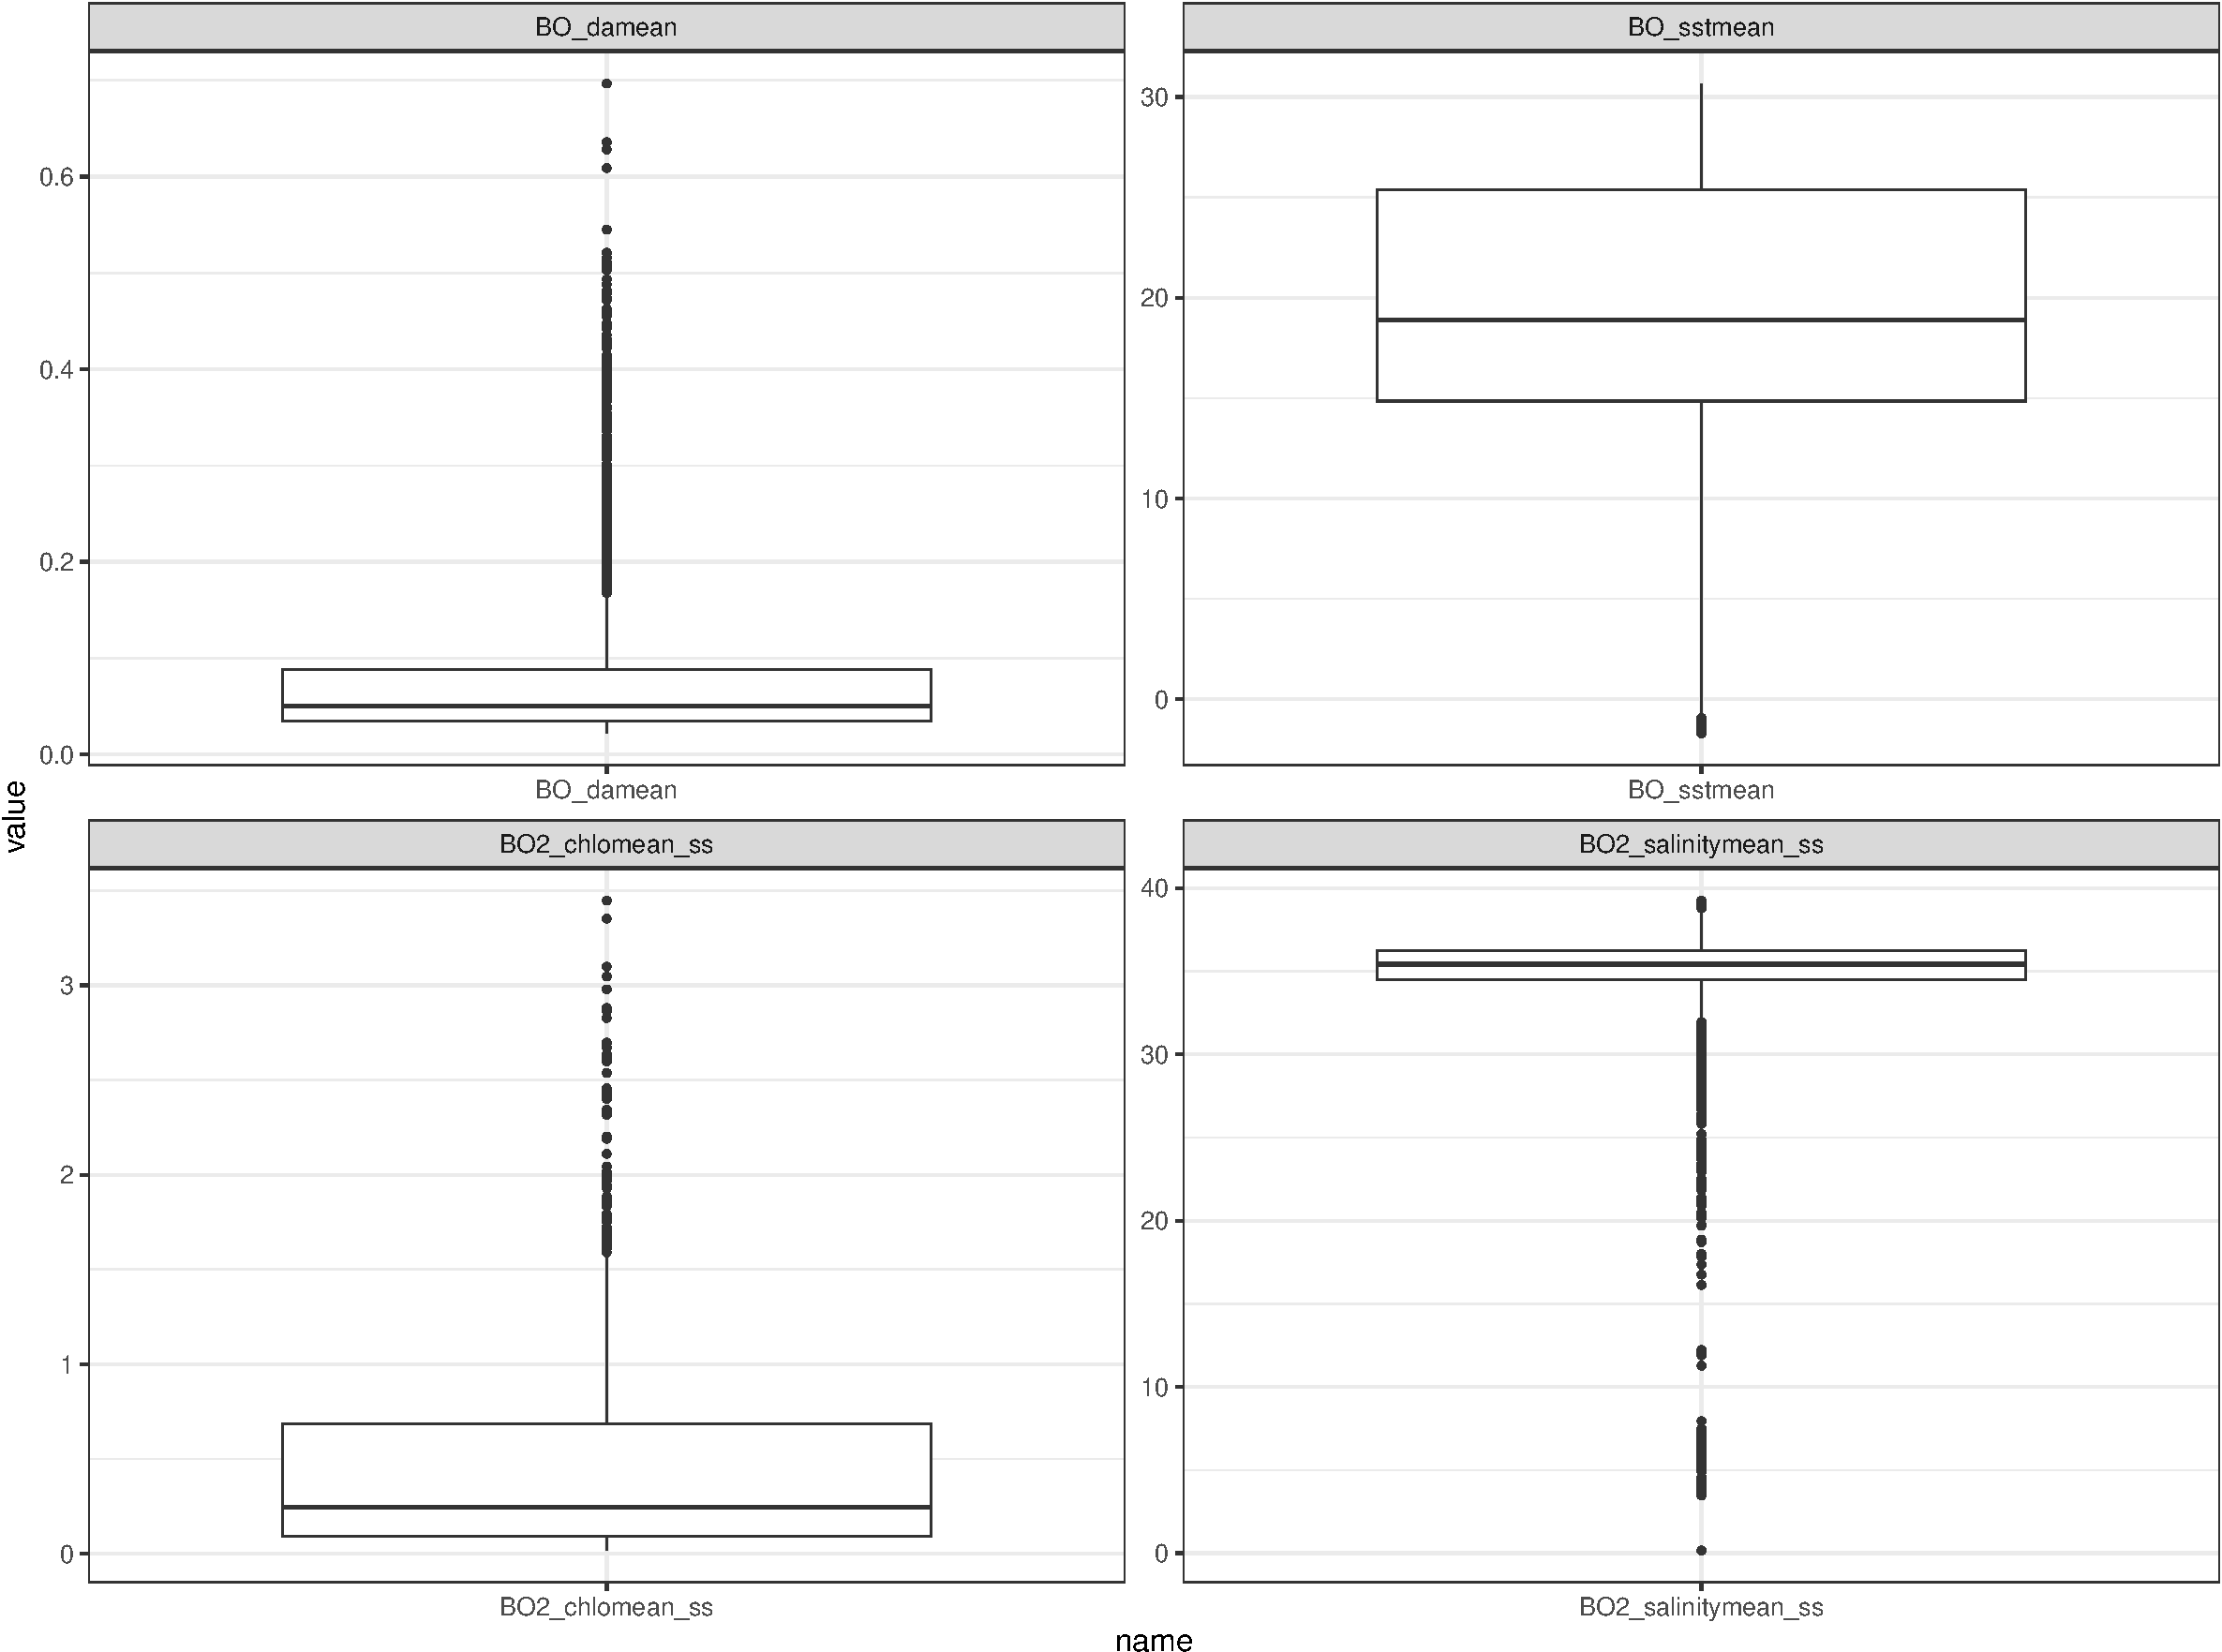
\includegraphics{_main_files/figure-latex/unnamed-chunk-49-1.pdf}

A more detailed analysis of the potential correlations can be conducted using the package \texttt{ggcorrplot}:

\begin{Shaded}
\begin{Highlighting}[]
\NormalTok{mat }\OtherTok{\textless{}{-}} \FunctionTok{cor}\NormalTok{(tmp, }\AttributeTok{use=}\StringTok{"complete.obs"}\NormalTok{) }
\NormalTok{p.mat }\OtherTok{\textless{}{-}} \FunctionTok{cor\_pmat}\NormalTok{(tmp)}

\FunctionTok{ggcorrplot}\NormalTok{(mat, }\AttributeTok{type =} \StringTok{"lower"}\NormalTok{, }\AttributeTok{lab=}\NormalTok{T, }\AttributeTok{p.mat =}\NormalTok{ p.mat)}
\end{Highlighting}
\end{Shaded}

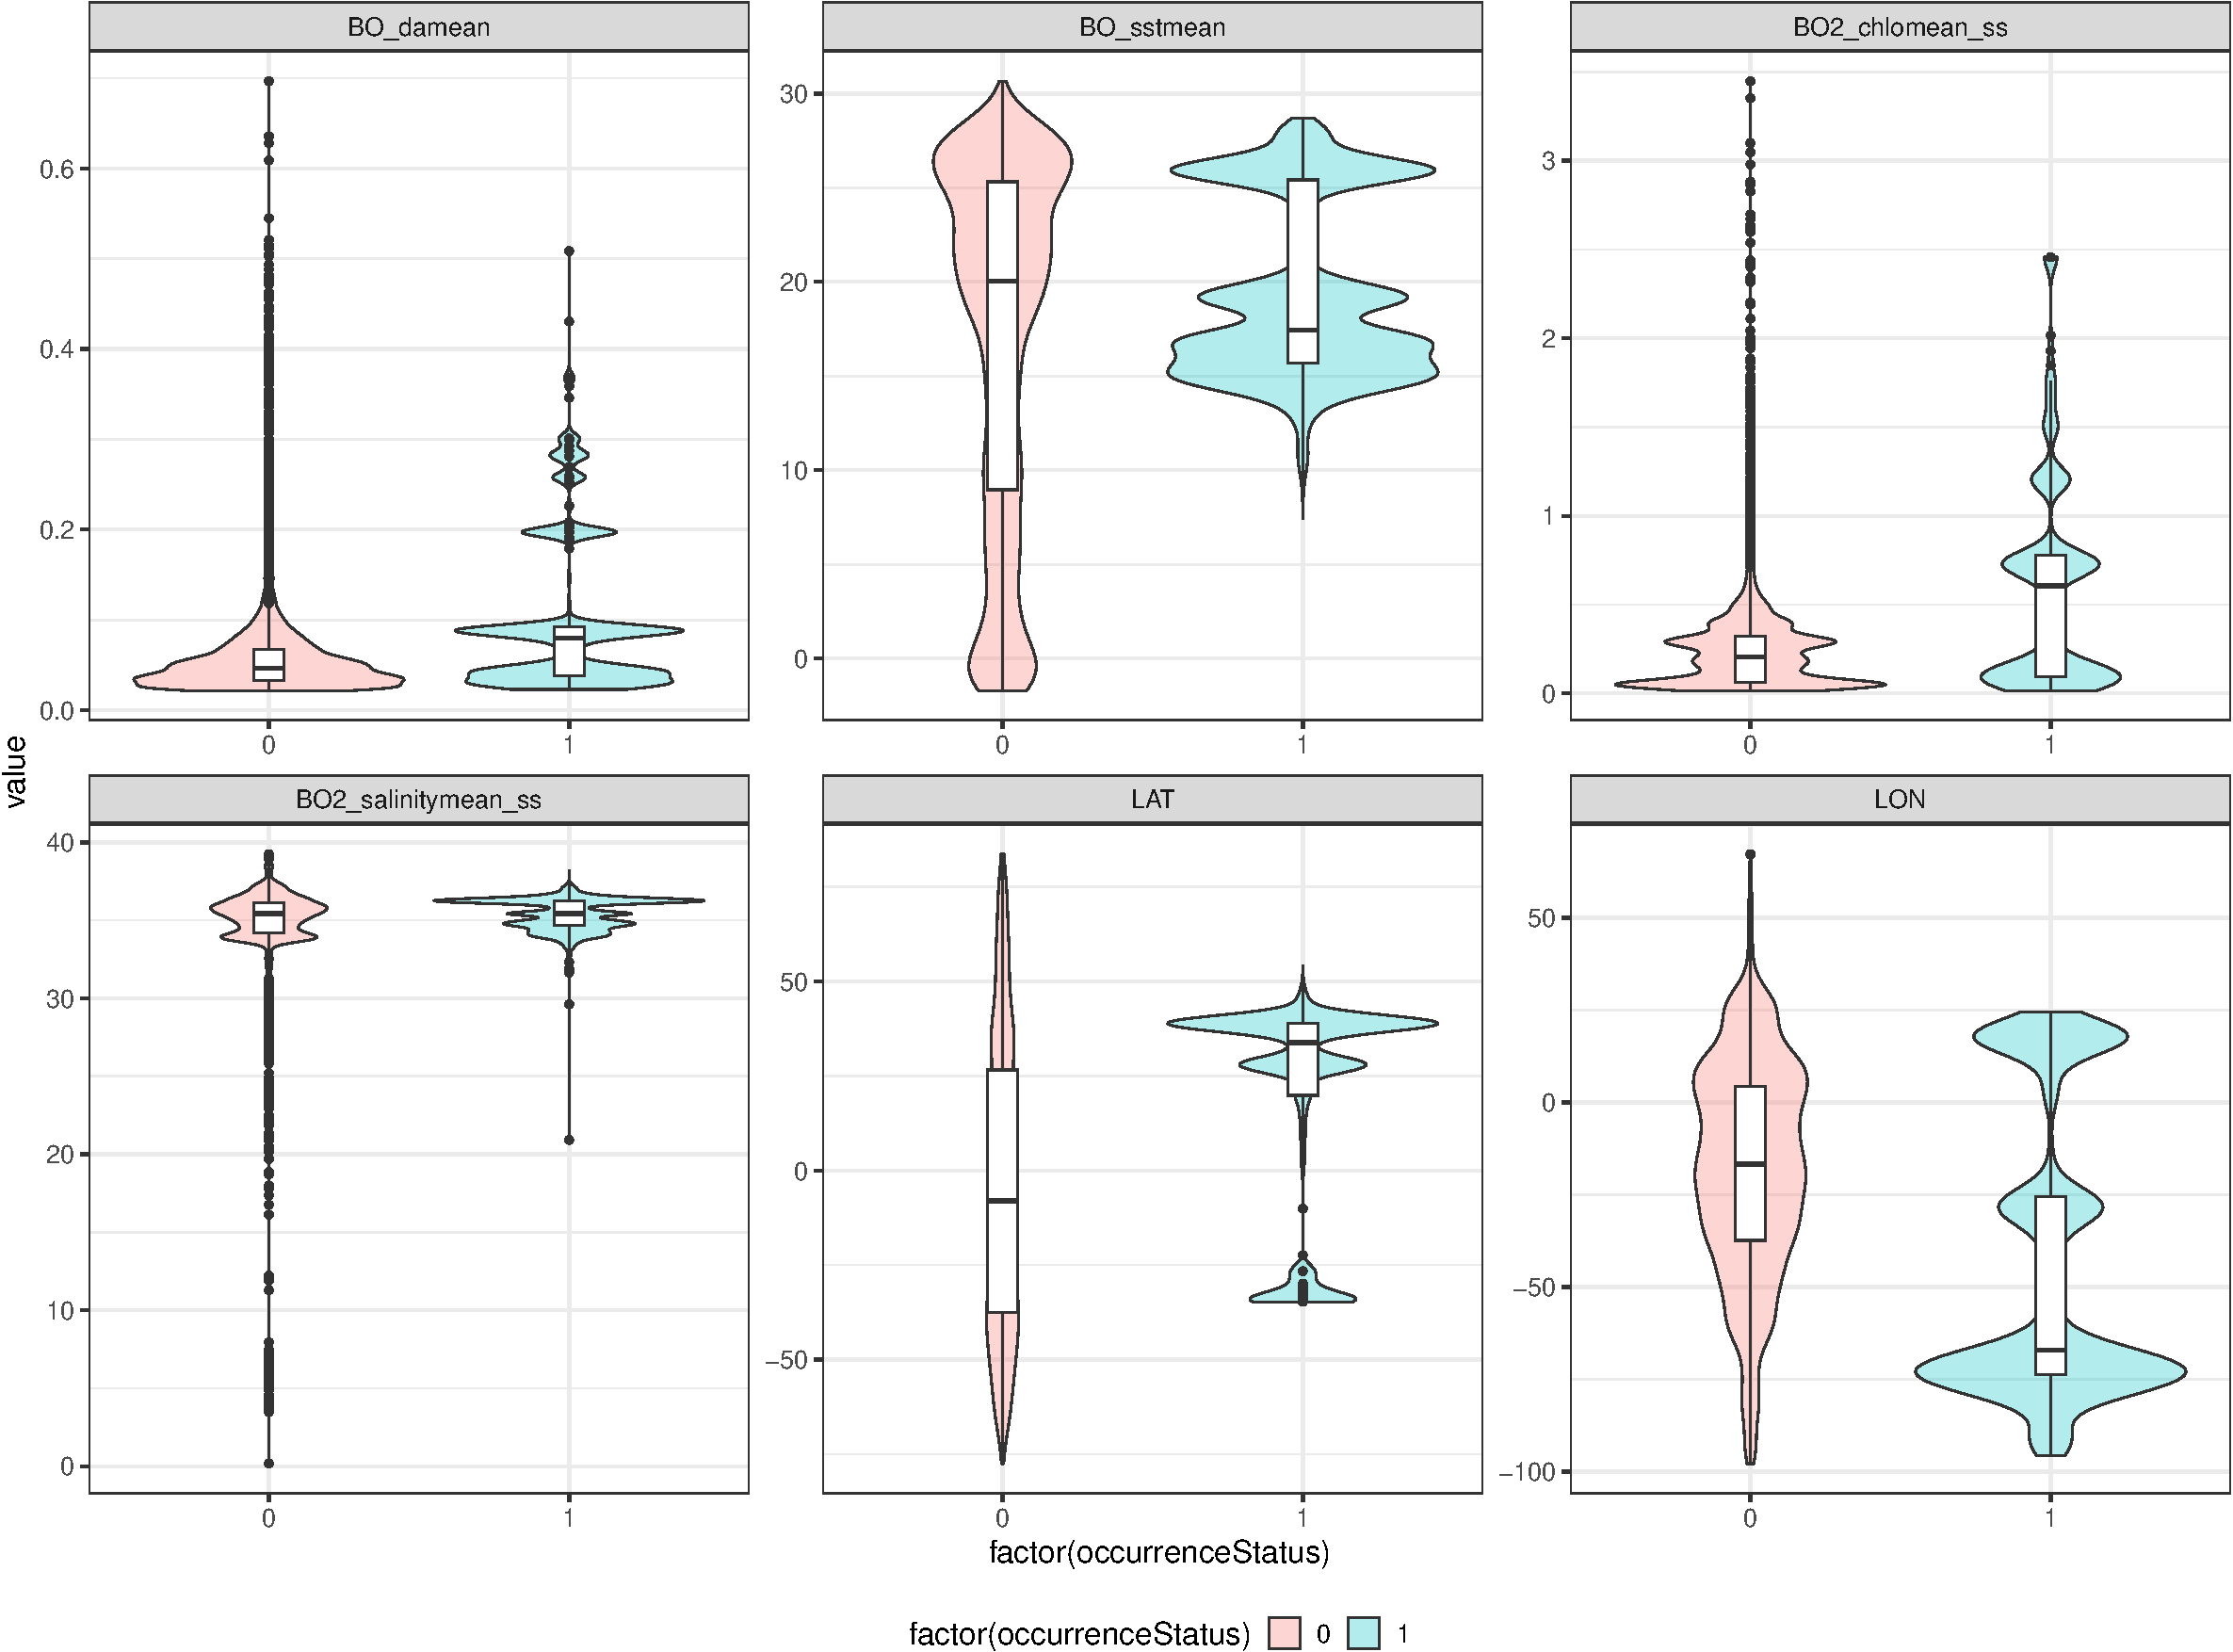
\includegraphics{_main_files/figure-latex/unnamed-chunk-50-1.pdf}

\hypertarget{variance-inflation-factor-vif}{%
\section{Variance Inflation Factor (VIF)}\label{variance-inflation-factor-vif}}

Furthermore, multicollinearity in regression analysis can be explored using the VIF (Variance Inflation Factor). The value of the VIF statistics indicate the level of multicollinearity with the rest of the variables:

\begin{itemize}
\tightlist
\item
  VIF equal to 1 = variables are not correlated
\item
  VIF between 1 and 5 = variables are moderately correlated
\item
  VIF greater than 5 = variables are highly correlated
\end{itemize}

There are several packages in \texttt{R} that allows to calculate the VIF statistics. In this case we use the package \texttt{HH}:

\begin{Shaded}
\begin{Highlighting}[]
\CommentTok{\# select variables for VIF calculation}
\NormalTok{v.table }\OtherTok{\textless{}{-}}\NormalTok{ data }\SpecialCharTok{\%\textgreater{}\%} 
\NormalTok{  dplyr}\SpecialCharTok{::}\FunctionTok{select}\NormalTok{ (BO2\_salinitymean\_ss, BO\_sstmean, BO2\_chlomean\_ss, BO\_damean)}

\CommentTok{\# get VIF results}
\NormalTok{out.vif }\OtherTok{\textless{}{-}} \FunctionTok{vif}\NormalTok{(v.table)}
\FunctionTok{sort}\NormalTok{(out.vif)}
\end{Highlighting}
\end{Shaded}

\begin{verbatim}
##          BO_sstmean BO2_salinitymean_ss     BO2_chlomean_ss           BO_damean 
##            1.375837            1.493366            5.270639            5.478410
\end{verbatim}

We remove the variable that has the highest VIF value and we test again the multicollinearity:

\begin{Shaded}
\begin{Highlighting}[]
\NormalTok{v.table }\OtherTok{\textless{}{-}}\NormalTok{ v.table }\SpecialCharTok{\%\textgreater{}\%} 
\NormalTok{  dplyr}\SpecialCharTok{::}\FunctionTok{select}\NormalTok{ (}\SpecialCharTok{{-}}\NormalTok{BO\_damean)}

\CommentTok{\#  get new VIF results}
\NormalTok{out.vif }\OtherTok{\textless{}{-}} \FunctionTok{vif}\NormalTok{(v.table)}
\FunctionTok{sort}\NormalTok{(out.vif)}
\end{Highlighting}
\end{Shaded}

\begin{verbatim}
##     BO2_chlomean_ss BO2_salinitymean_ss          BO_sstmean 
##            1.136295            1.222233            1.300901
\end{verbatim}

Now all the variables have VIF values that are acceptable. So, we proceed to remove BO\_damean (Diffuse attenuation coefficient at 490 nm). And save the selected variables for the next modelling stages:

\begin{Shaded}
\begin{Highlighting}[]
\NormalTok{data }\OtherTok{\textless{}{-}}\NormalTok{ data }\SpecialCharTok{\%\textgreater{}\%}\NormalTok{ dplyr}\SpecialCharTok{::}\FunctionTok{select}\NormalTok{ (}\SpecialCharTok{{-}}\NormalTok{BO\_damean)}
\end{Highlighting}
\end{Shaded}

We save the dataset as our output for modelling

\begin{Shaded}
\begin{Highlighting}[]
\FunctionTok{save}\NormalTok{(}\AttributeTok{list=}\StringTok{"data"}\NormalTok{, }\AttributeTok{file=}\StringTok{"data/outputs\_for\_modelling/PAdata\_with\_env.RData"}\NormalTok{)}
\end{Highlighting}
\end{Shaded}

\hypertarget{shape-constrained-generalized-additive-models}{%
\section{Shape Constrained-Generalized Additive Models}\label{shape-constrained-generalized-additive-models}}

In order to fit SDM in agreement with the ecological niche theory, the proposed Shape-Constrained Generalized Additive Models (SC-GAMs) in \citep{citores_etal_2020} are fitted in this section. SC-GAMs are based on Generalized Additive Models, allowing us to impose shape-constraints to the linear predictor function. The R package SCAM implements the general framework developed by \citep{pya_etal_2015} using shape-constrained P-splines. Monotonicity and concavity/convexity constraints can be imposed on the sign of the first and/or the second derivatives of the smooth terms. For fitting Species Distribution Models in agreement with the ecological niche theory, we imposed concavity constraints (\(f''(x) \le 0\)), so that the response can presents at most a single mode.

Alternatively, the R package \texttt{mboost} fits SC-GAMs using boosting methods. We are not going to develop this alternative here.

First we load the list of required libraries.

\begin{Shaded}
\begin{Highlighting}[]
\NormalTok{requiredPackages }\OtherTok{\textless{}{-}} \FunctionTok{c}\NormalTok{(}
  \CommentTok{\#GENERAL USE LIBRARIES {-}{-}{-}{-}{-}{-}{-}{-}\#}
  \StringTok{"here"}\NormalTok{, }\CommentTok{\# Library for reproducible workflow}
  \StringTok{"rstudioapi"}\NormalTok{,  }\CommentTok{\# Library for reproducible workflow}
  \StringTok{"stringr"}\NormalTok{,}
  \StringTok{"RColorBrewer"}\NormalTok{,  }
  \StringTok{"ggplot2"}\NormalTok{,}
  \StringTok{"dplyr"}\NormalTok{,}
  
  \CommentTok{\#SPATIAL DATA {-}{-}{-}{-}{-}{-}{-}{-}\#}
  \StringTok{"rgdal"}\NormalTok{,}
  \StringTok{"fields"}\NormalTok{,}
  \StringTok{"maps"}\NormalTok{ ,}
  \StringTok{"raster"}\NormalTok{,}

  \CommentTok{\#MODEL FIT {-}{-}{-}{-}{-}{-}{-}{-}\#}
  \StringTok{"scam"}\NormalTok{,}
  \StringTok{"plotmo"}\NormalTok{,}
  \StringTok{"SDMTools"}\NormalTok{,}
  \StringTok{"pkgbuild"}\NormalTok{,}
  \StringTok{"dismo"}
\NormalTok{  )}
\end{Highlighting}
\end{Shaded}

We run a function to install the required packages that are not in our system and load all the required packages.

\begin{Shaded}
\begin{Highlighting}[]
\NormalTok{install\_load\_function }\OtherTok{\textless{}{-}} \ControlFlowTok{function}\NormalTok{(pkg)\{}
\NormalTok{  new.pkg }\OtherTok{\textless{}{-}}\NormalTok{ pkg[}\SpecialCharTok{!}\NormalTok{(pkg }\SpecialCharTok{\%in\%} \FunctionTok{installed.packages}\NormalTok{()[, }\StringTok{"Package"}\NormalTok{])]}
  \ControlFlowTok{if}\NormalTok{ (}\FunctionTok{length}\NormalTok{(new.pkg))}
    \FunctionTok{install.packages}\NormalTok{(new.pkg, }\AttributeTok{dependencies =} \ConstantTok{TRUE}\NormalTok{)}
  \FunctionTok{sapply}\NormalTok{(pkg, require, }\AttributeTok{character.only =} \ConstantTok{TRUE}\NormalTok{)}
\NormalTok{\}}

\FunctionTok{install\_load\_function}\NormalTok{(requiredPackages)}
\end{Highlighting}
\end{Shaded}

\begin{verbatim}
##         here   rstudioapi      stringr RColorBrewer      ggplot2        dplyr 
##         TRUE         TRUE         TRUE         TRUE         TRUE         TRUE 
##        rgdal       fields         maps       raster         scam       plotmo 
##         TRUE         TRUE         TRUE         TRUE         TRUE         TRUE 
##     SDMTools     pkgbuild        dismo 
##         TRUE         TRUE         TRUE
\end{verbatim}

Install and load SDMTools. You need to manually install RTools installed: \url{https://cran.r-project.org/bin/windows/Rtools/history.html}

\begin{Shaded}
\begin{Highlighting}[]
\CommentTok{\# find\_rtools()}
\CommentTok{\# }
\CommentTok{\# install.packages("remotes")}
\CommentTok{\# remotes::install\_version("SDMTools", version = "1.1{-}221.2")}
\end{Highlighting}
\end{Shaded}

We define some overall settings.

\begin{Shaded}
\begin{Highlighting}[]
\CommentTok{\# General settings for ggplot (black{-}white background, larger base\_size)}
\FunctionTok{theme\_set}\NormalTok{(}\FunctionTok{theme\_bw}\NormalTok{(}\AttributeTok{base\_size =} \DecValTok{16}\NormalTok{))}
\end{Highlighting}
\end{Shaded}

\hypertarget{model-fit}{%
\section{Model fit}\label{model-fit}}

We set the working directory to the folder where the current script is located and we load the dataset (PAdata\_with\_env.Rdata) containing the presence-absence data together with the environmental data.

\begin{Shaded}
\begin{Highlighting}[]
\FunctionTok{load}\NormalTok{(here}\SpecialCharTok{::}\FunctionTok{here}\NormalTok{ (}\StringTok{"data"}\NormalTok{, }\StringTok{"outputs\_for\_modelling"}\NormalTok{, }\StringTok{"PAdata\_with\_env.Rdata"}\NormalTok{))}
\end{Highlighting}
\end{Shaded}

To fit a logistic regression model in the SC-GAMs framework, we use the scam function, where we set the binomial family with the logit link function. Our response variable is the presence-absence data and the selected three explanatory variables are the SST, chlorophyll and salinity. Each variable is included in the model through an spline function where the concavity constraint is set using bs=``cv''. The details about this option can be found in the section ``Constructor for concave P-splines in SCAMs'' of the SCAM manual (\url{https://cran.r-project.org/web/packages/scam/scam.pdf}). The number of knots (k) is fixed at 8 in this example for a good balance between flexibility and computation time.

\textbf{UNIVARIATE MODELS}

Before fitting the model with the selected three environmental variables, we can fit univariate model as follows.

We fit the univariate model for SST, we print the summary of the model fit, and look at the fitted curve in the response scale.

\begin{Shaded}
\begin{Highlighting}[]
\NormalTok{model\_sst }\OtherTok{\textless{}{-}} \FunctionTok{scam}\NormalTok{ (occurrenceStatus }\SpecialCharTok{\textasciitilde{}}  \FunctionTok{s}\NormalTok{(BO\_sstmean, }\AttributeTok{k=}\DecValTok{8}\NormalTok{,}\AttributeTok{bs=}\StringTok{"cv"}\NormalTok{), }\AttributeTok{family=}\FunctionTok{binomial}\NormalTok{(}\AttributeTok{link=}\StringTok{"logit"}\NormalTok{), }\AttributeTok{data=}\NormalTok{data)}
\FunctionTok{summary}\NormalTok{(model\_sst)}
\end{Highlighting}
\end{Shaded}

\begin{verbatim}
## 
## Family: binomial 
## Link function: logit 
## 
## Formula:
## occurrenceStatus ~ s(BO_sstmean, k = 8, bs = "cv")
## 
## Parametric coefficients:
##             Estimate Std. Error z value Pr(>|z|)    
## (Intercept)  -47.180      2.182  -21.62   <2e-16 ***
## ---
## Signif. codes:  0 '***' 0.001 '**' 0.01 '*' 0.05 '.' 0.1 ' ' 1
## 
## Approximate significance of smooth terms:
##               edf Ref.df Chi.sq p-value    
## s(BO_sstmean)   2      2   1111  <2e-16 ***
## ---
## Signif. codes:  0 '***' 0.001 '**' 0.01 '*' 0.05 '.' 0.1 ' ' 1
## 
## R-sq.(adj) =  0.2607   Deviance explained = 23.1%
## UBRE score = 0.066363  Scale est. = 1         n = 29661
\end{verbatim}

\begin{Shaded}
\begin{Highlighting}[]
\FunctionTok{plotmo}\NormalTok{(model\_sst,}\AttributeTok{level =} \FloatTok{0.95}\NormalTok{, }\AttributeTok{pt.col=}\DecValTok{8}\NormalTok{)}
\end{Highlighting}
\end{Shaded}

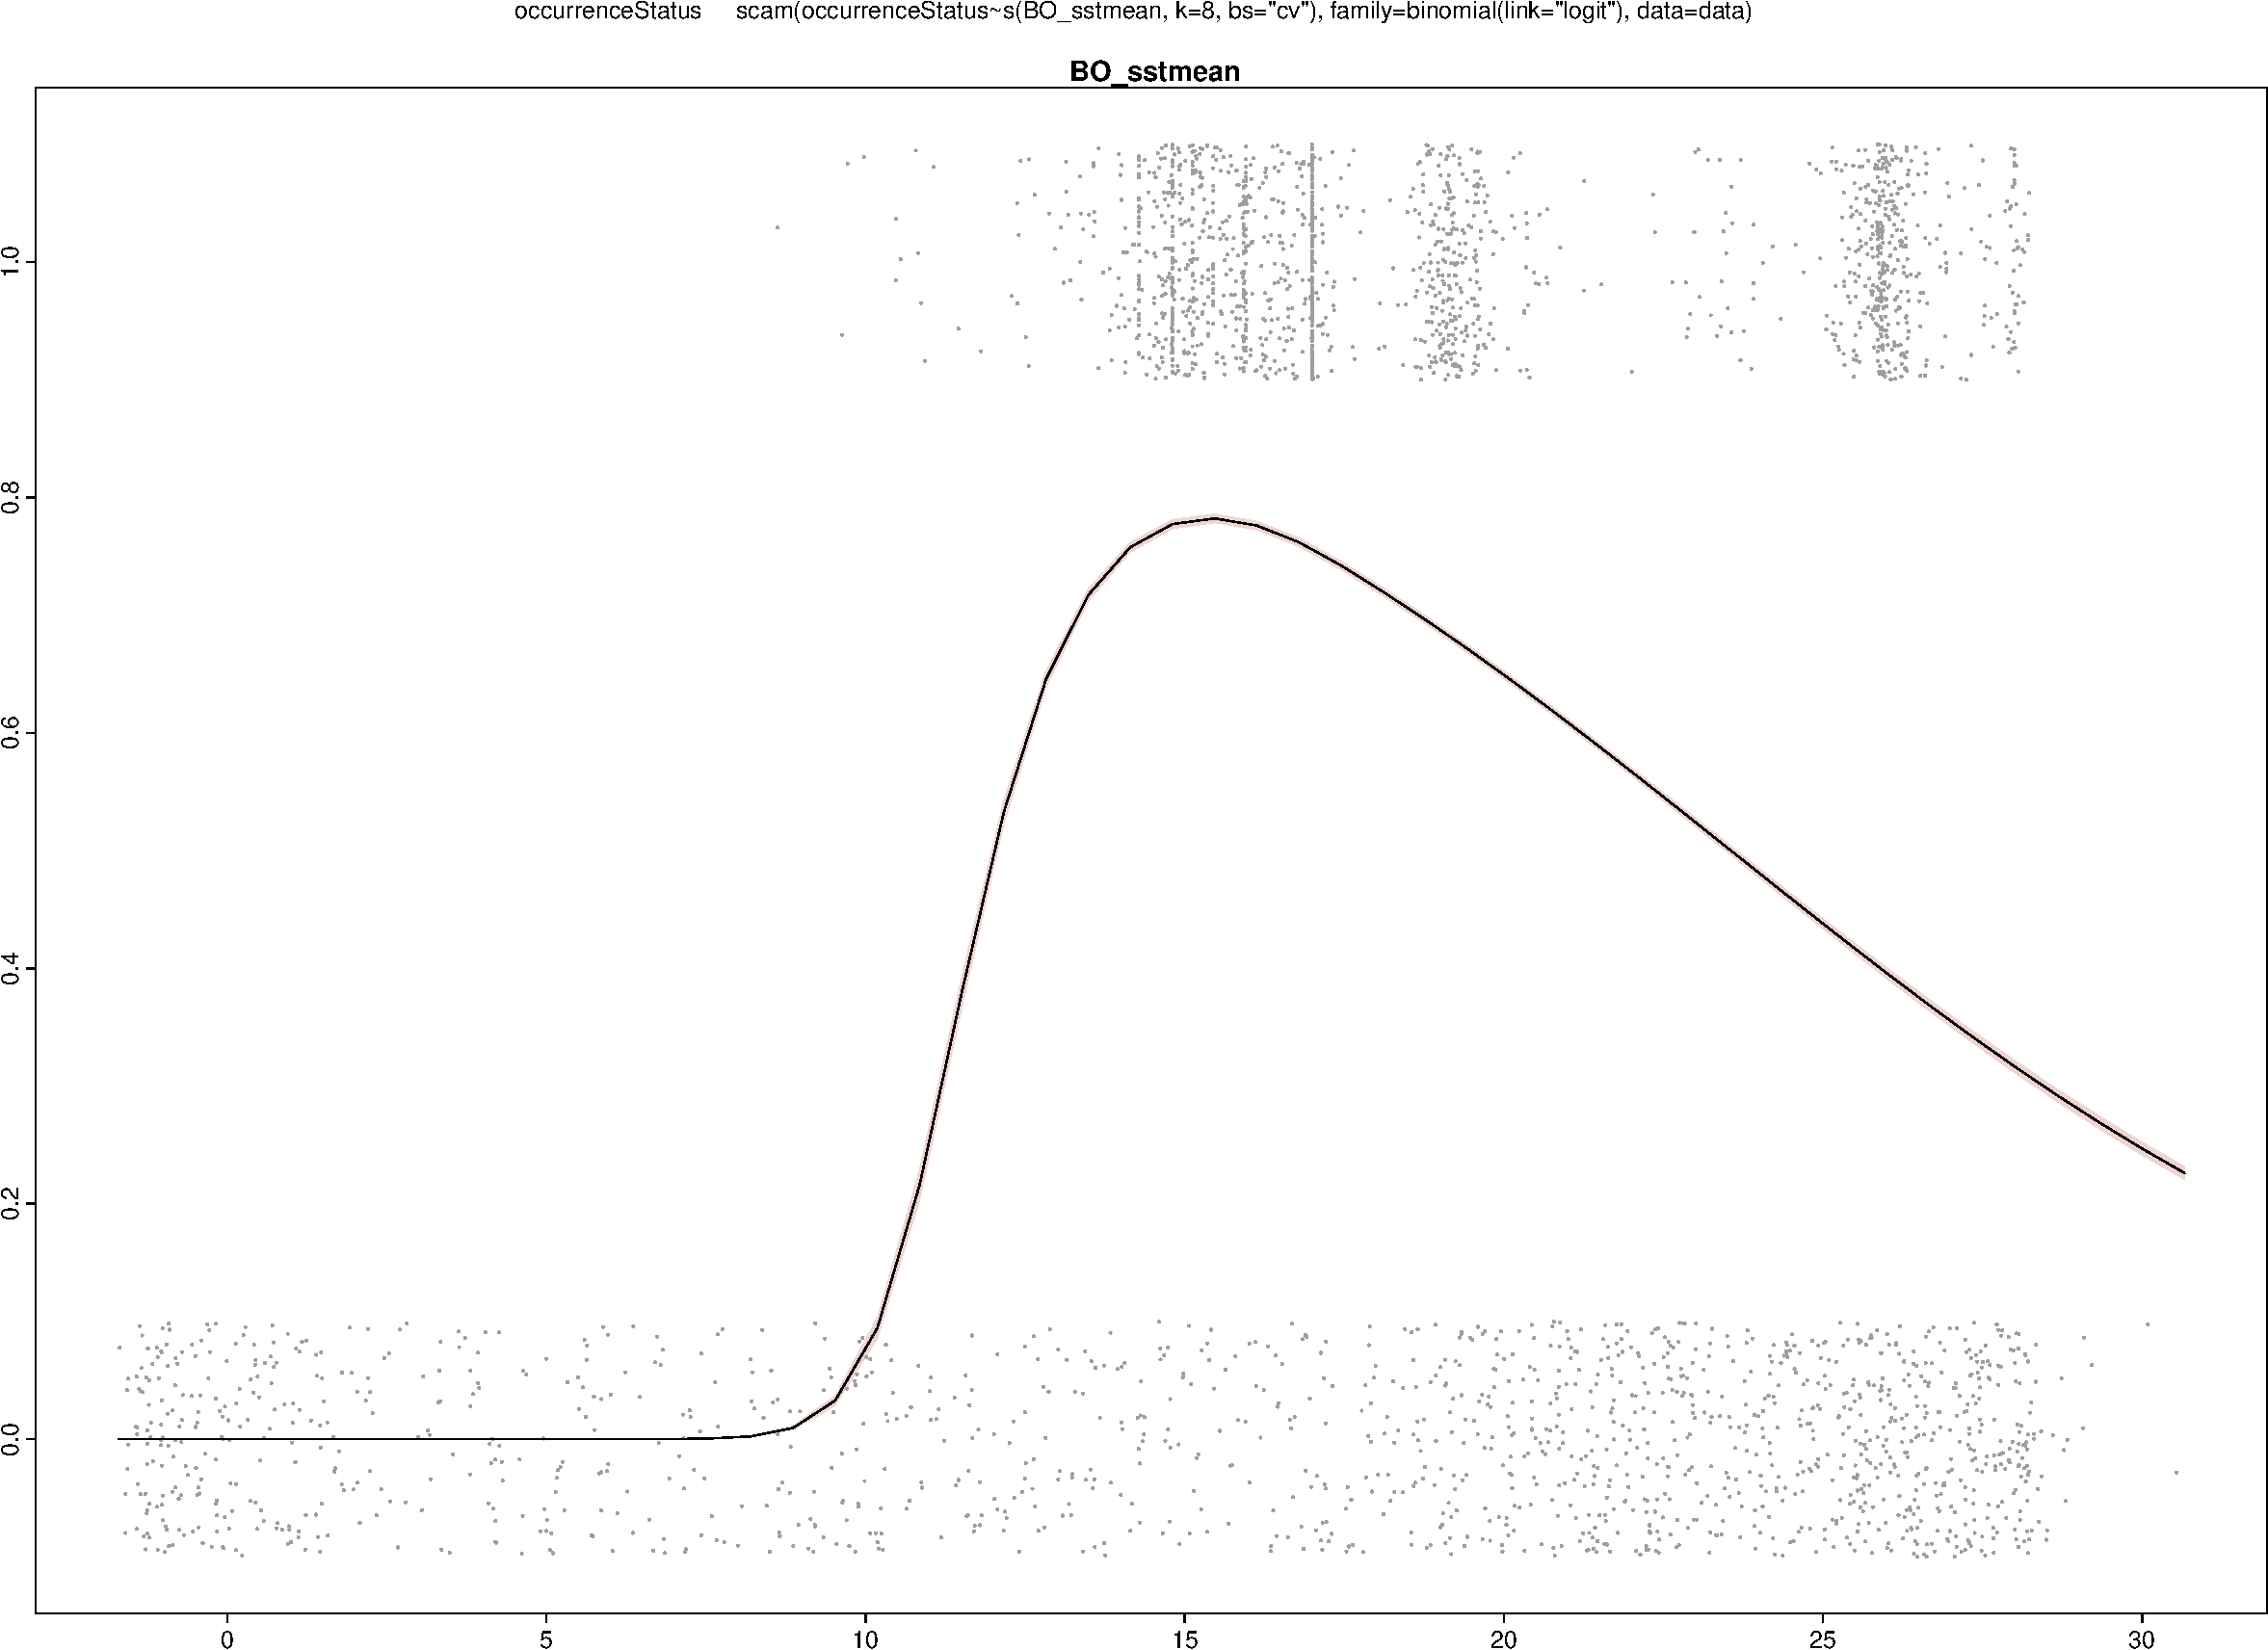
\includegraphics{_main_files/figure-latex/unnamed-chunk-60-1.pdf}

We repeat the same steps for the rest of the variables.

\begin{Shaded}
\begin{Highlighting}[]
\NormalTok{model\_chl }\OtherTok{\textless{}{-}} \FunctionTok{scam}\NormalTok{ (occurrenceStatus }\SpecialCharTok{\textasciitilde{}}  \FunctionTok{s}\NormalTok{(BO2\_chlomean\_ss, }\AttributeTok{k=}\DecValTok{8}\NormalTok{,}\AttributeTok{bs=}\StringTok{"cv"}\NormalTok{), }\AttributeTok{family=}\FunctionTok{binomial}\NormalTok{(}\AttributeTok{link=}\StringTok{"logit"}\NormalTok{), }\AttributeTok{data=}\NormalTok{data)}
\FunctionTok{summary}\NormalTok{(model\_chl)}
\end{Highlighting}
\end{Shaded}

\begin{verbatim}
## 
## Family: binomial 
## Link function: logit 
## 
## Formula:
## occurrenceStatus ~ s(BO2_chlomean_ss, k = 8, bs = "cv")
## 
## Parametric coefficients:
##             Estimate Std. Error z value Pr(>|z|)    
## (Intercept)  -2.3878     0.0417  -57.27   <2e-16 ***
## ---
## Signif. codes:  0 '***' 0.001 '**' 0.01 '*' 0.05 '.' 0.1 ' ' 1
## 
## Approximate significance of smooth terms:
##                    edf Ref.df Chi.sq p-value    
## s(BO2_chlomean_ss)   1      1   3263  <2e-16 ***
## ---
## Signif. codes:  0 '***' 0.001 '**' 0.01 '*' 0.05 '.' 0.1 ' ' 1
## Rank: 7/8
## 
## R-sq.(adj) =  0.1546   Deviance explained = 12.4%
## UBRE score = 0.21423  Scale est. = 1         n = 29661
\end{verbatim}

\begin{Shaded}
\begin{Highlighting}[]
\FunctionTok{plotmo}\NormalTok{(model\_chl,}\AttributeTok{level =} \FloatTok{0.95}\NormalTok{, }\AttributeTok{pt.col=}\DecValTok{8}\NormalTok{)}
\end{Highlighting}
\end{Shaded}

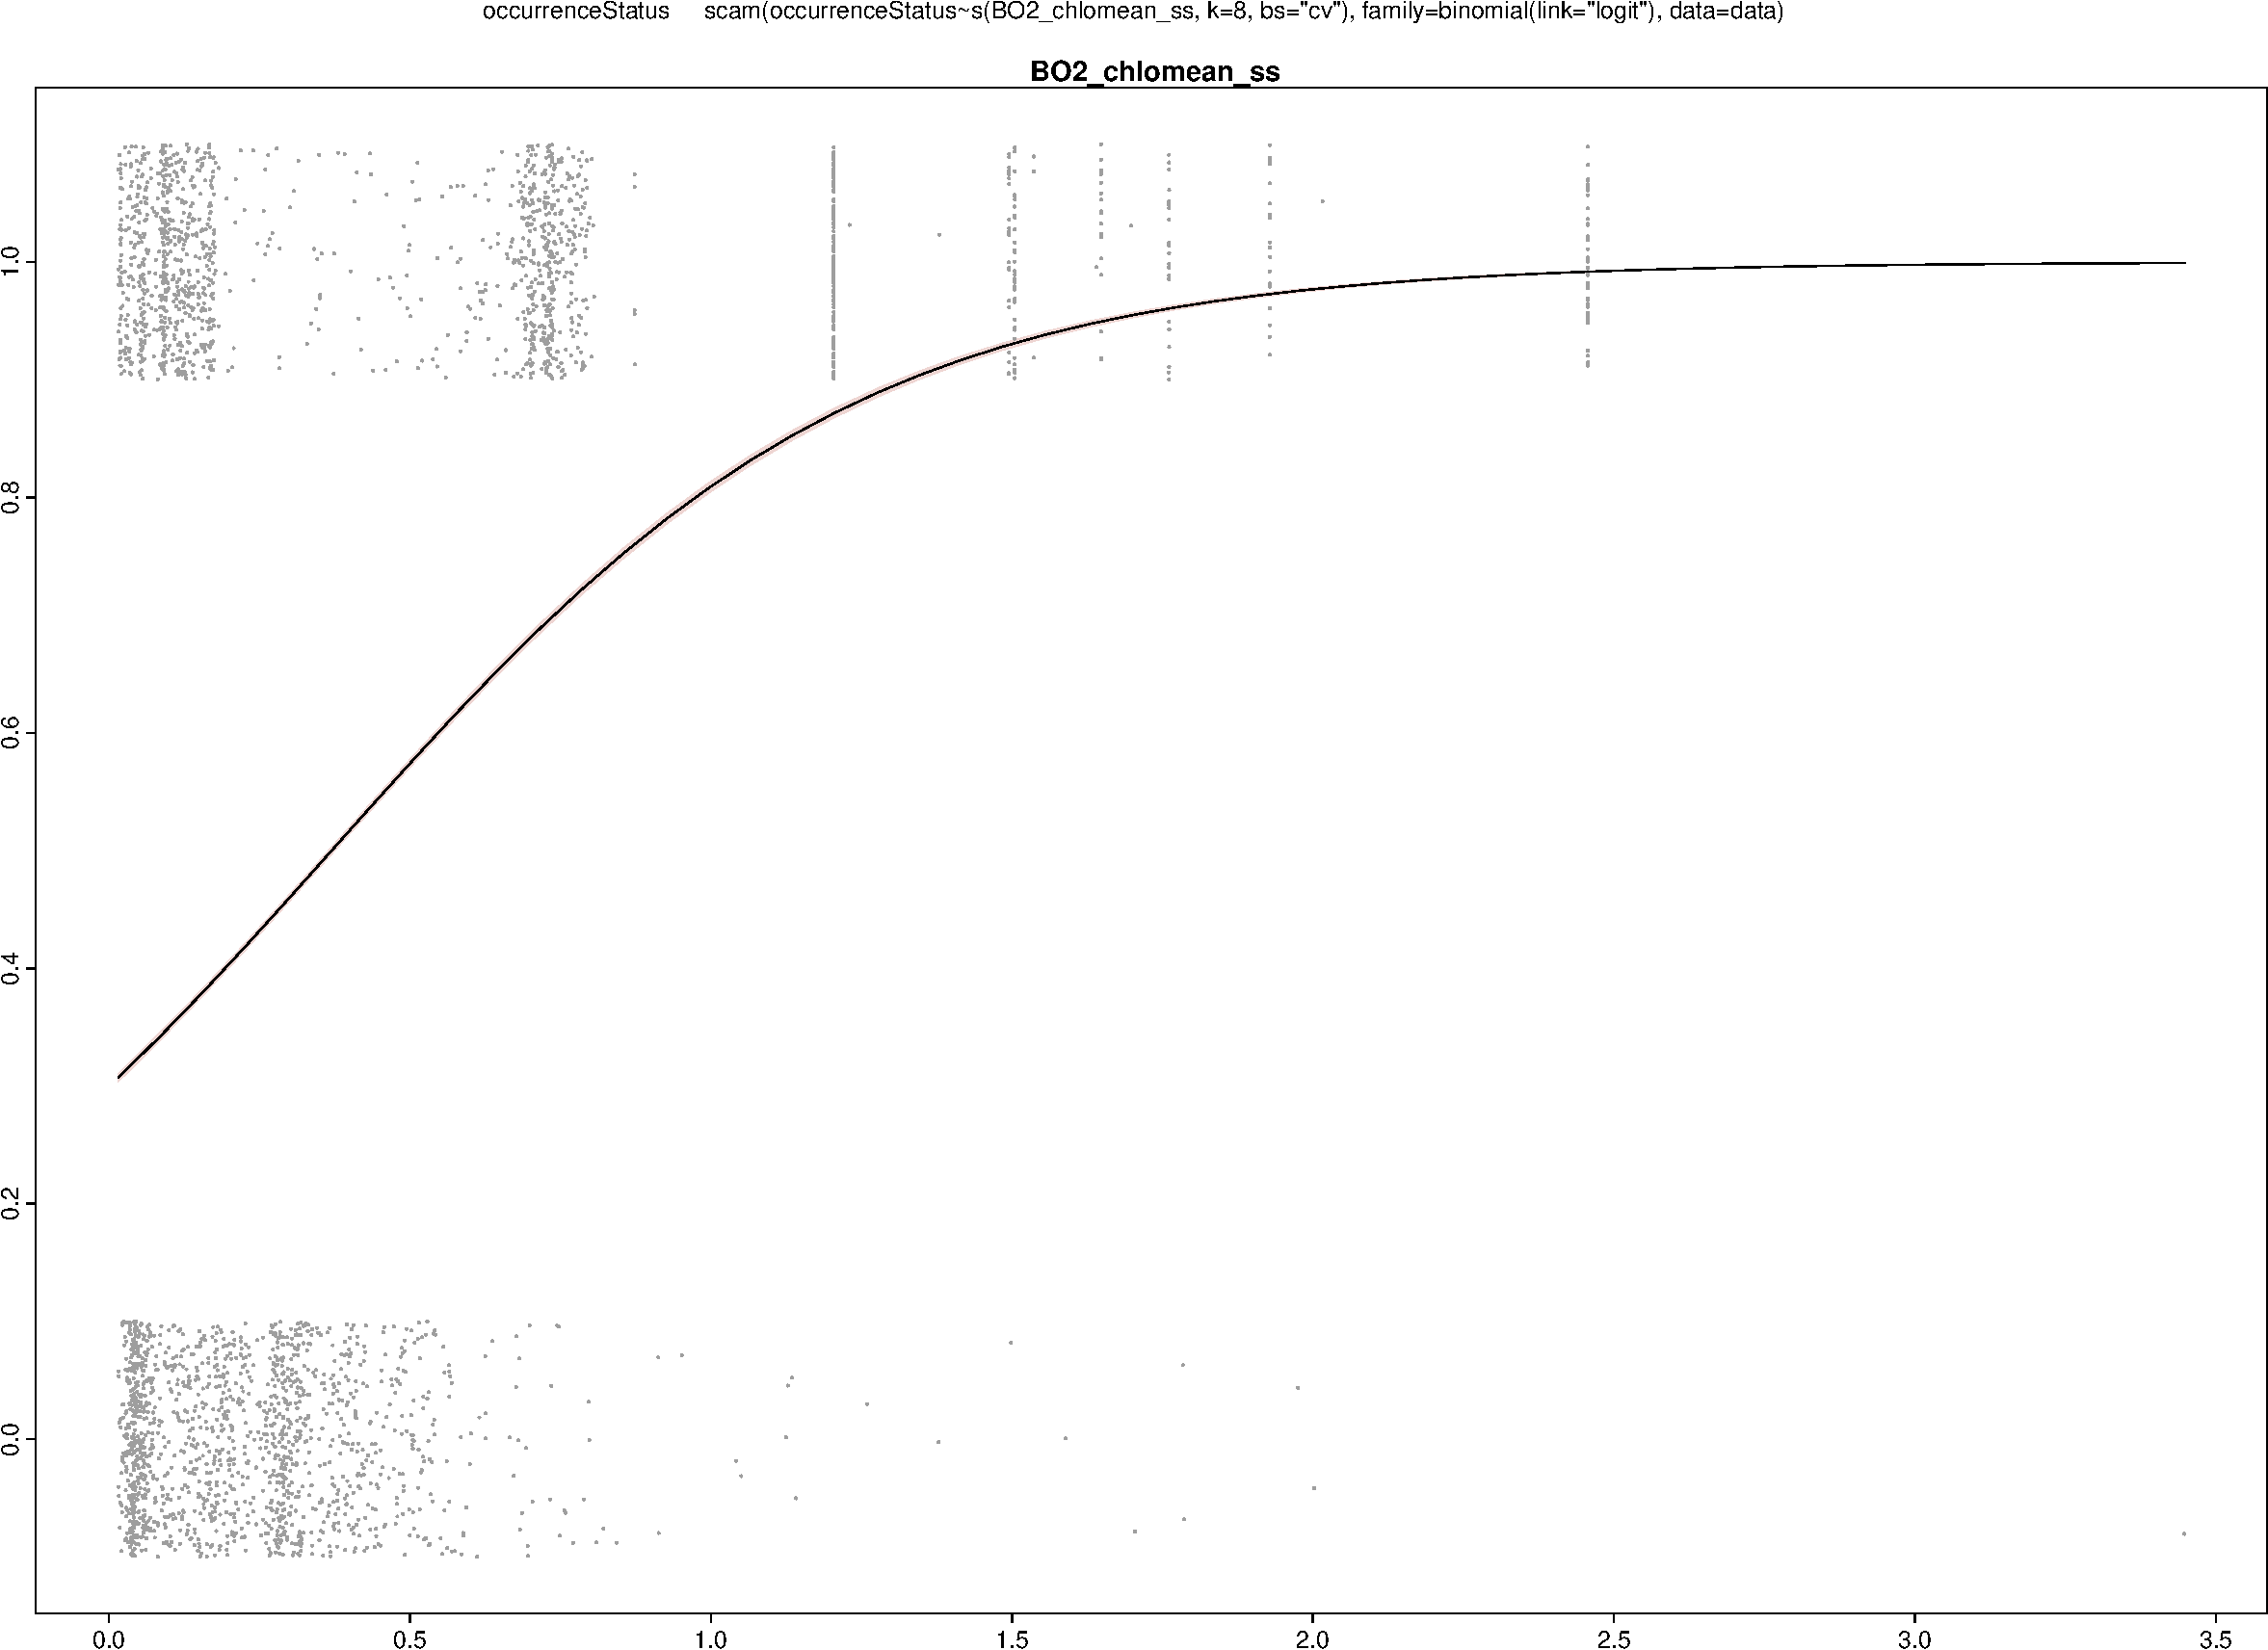
\includegraphics{_main_files/figure-latex/unnamed-chunk-61-1.pdf}

Due to convergence issues, sometimes it is necessary to fix the smoothing parameter (sp) at small value, i.e.~\(10^{-5}\), as here when introducing salinity as an explanatory variable. If no value is provided, the smoothing parameter is estimated within the model.

\begin{Shaded}
\begin{Highlighting}[]
\NormalTok{model\_sal }\OtherTok{\textless{}{-}} \FunctionTok{scam}\NormalTok{ (occurrenceStatus }\SpecialCharTok{\textasciitilde{}}  \FunctionTok{s}\NormalTok{(BO2\_salinitymean\_ss, }\AttributeTok{k=}\DecValTok{8}\NormalTok{,}\AttributeTok{bs=}\StringTok{"cv"}\NormalTok{), }\AttributeTok{family=}\FunctionTok{binomial}\NormalTok{(}\AttributeTok{link=}\StringTok{"logit"}\NormalTok{), }\AttributeTok{data=}\NormalTok{data,}\AttributeTok{sp=}\FloatTok{0.00001}\NormalTok{)}
\FunctionTok{summary}\NormalTok{(model\_sal)}
\end{Highlighting}
\end{Shaded}

\begin{verbatim}
## 
## Family: binomial 
## Link function: logit 
## 
## Formula:
## occurrenceStatus ~ s(BO2_salinitymean_ss, k = 8, bs = "cv")
## 
## Parametric coefficients:
##             Estimate Std. Error z value Pr(>|z|)    
## (Intercept)  -50.076      1.853  -27.02   <2e-16 ***
## ---
## Signif. codes:  0 '***' 0.001 '**' 0.01 '*' 0.05 '.' 0.1 ' ' 1
## 
## Approximate significance of smooth terms:
##                        edf Ref.df Chi.sq p-value    
## s(BO2_salinitymean_ss)   2      2  913.1  <2e-16 ***
## ---
## Signif. codes:  0 '***' 0.001 '**' 0.01 '*' 0.05 '.' 0.1 ' ' 1
## 
## R-sq.(adj) =  0.0514   Deviance explained = 4.38%
##   Scale est. = 1         n = 29661
\end{verbatim}

\begin{Shaded}
\begin{Highlighting}[]
\FunctionTok{plotmo}\NormalTok{(model\_sal,}\AttributeTok{level =} \FloatTok{0.95}\NormalTok{, }\AttributeTok{pt.col=}\DecValTok{8}\NormalTok{)}
\end{Highlighting}
\end{Shaded}

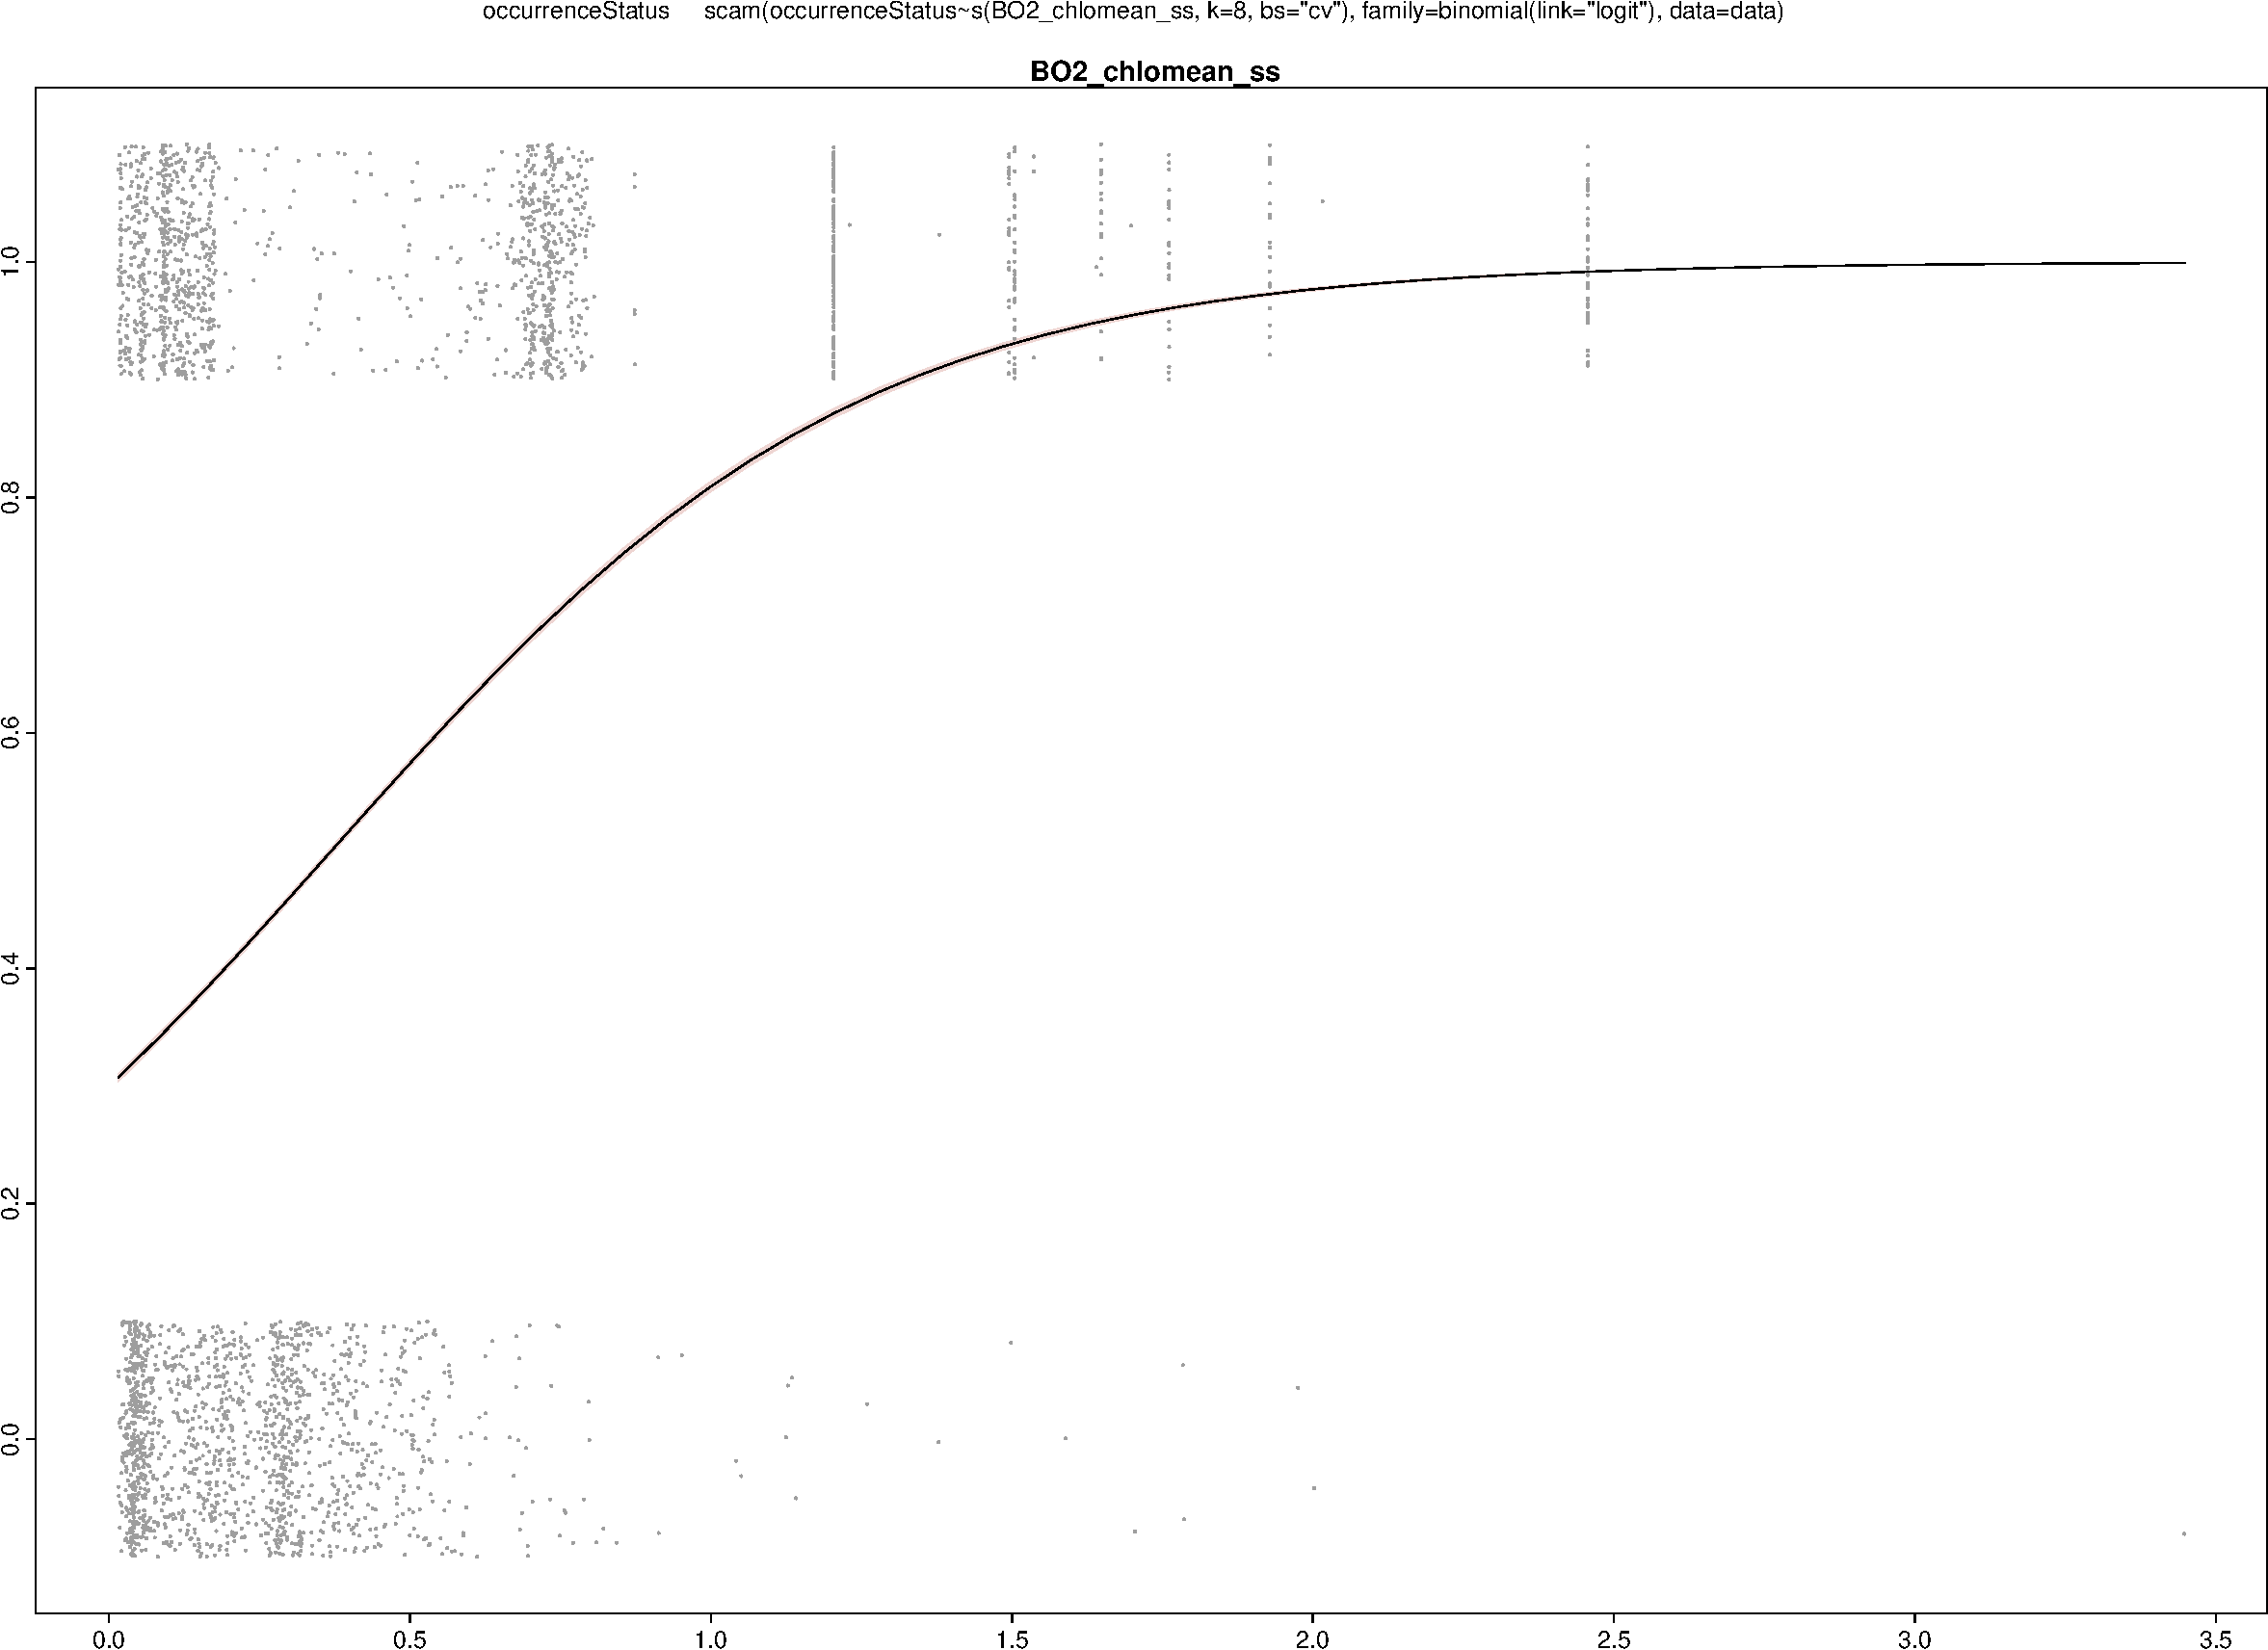
\includegraphics{_main_files/figure-latex/unnamed-chunk-62-1.pdf}

\textbf{MODEL WITH ALL VARIABLES}

Now we fit the model including the three selected variables.

\begin{Shaded}
\begin{Highlighting}[]
\NormalTok{model }\OtherTok{\textless{}{-}} \FunctionTok{scam}\NormalTok{ (occurrenceStatus }\SpecialCharTok{\textasciitilde{}}  \FunctionTok{s}\NormalTok{(BO\_sstmean, }\AttributeTok{k=}\DecValTok{8}\NormalTok{,}\AttributeTok{bs=}\StringTok{"cv"}\NormalTok{)}\SpecialCharTok{+} \FunctionTok{s}\NormalTok{(BO2\_salinitymean\_ss, }\AttributeTok{k=}\DecValTok{8}\NormalTok{,}\AttributeTok{bs=}\StringTok{"cv"}\NormalTok{)}\SpecialCharTok{+}\FunctionTok{s}\NormalTok{(BO2\_chlomean\_ss, }\AttributeTok{k=}\DecValTok{8}\NormalTok{,}\AttributeTok{bs=}\StringTok{"cv"}\NormalTok{), }\AttributeTok{family=}\FunctionTok{binomial}\NormalTok{(}\AttributeTok{link=}\StringTok{"logit"}\NormalTok{), }\AttributeTok{data=}\NormalTok{data,}\AttributeTok{sp=}\FunctionTok{rep}\NormalTok{(}\FloatTok{0.00001}\NormalTok{,}\DecValTok{3}\NormalTok{))}
\FunctionTok{summary}\NormalTok{(model)}
\end{Highlighting}
\end{Shaded}

\begin{verbatim}
## 
## Family: binomial 
## Link function: logit 
## 
## Formula:
## occurrenceStatus ~ s(BO_sstmean, k = 8, bs = "cv") + s(BO2_salinitymean_ss, 
##     k = 8, bs = "cv") + s(BO2_chlomean_ss, k = 8, bs = "cv")
## 
## Parametric coefficients:
##             Estimate Std. Error z value Pr(>|z|)
## (Intercept)   -56.08      45.69  -1.227     0.22
## 
## Approximate significance of smooth terms:
##                          edf Ref.df Chi.sq p-value    
## s(BO_sstmean)          3.936  3.999  772.6  <2e-16 ***
## s(BO2_salinitymean_ss) 2.001  2.001  191.4  <2e-16 ***
## s(BO2_chlomean_ss)     3.985  4.003 1820.7  <2e-16 ***
## ---
## Signif. codes:  0 '***' 0.001 '**' 0.01 '*' 0.05 '.' 0.1 ' ' 1
## 
## R-sq.(adj) =  0.3488   Deviance explained = 31.9%
##   Scale est. = 1         n = 29661
\end{verbatim}

\begin{Shaded}
\begin{Highlighting}[]
\FunctionTok{plotmo}\NormalTok{(model,}\AttributeTok{level =} \FloatTok{0.95}\NormalTok{, }\AttributeTok{pt.col=}\DecValTok{8}\NormalTok{)}
\end{Highlighting}
\end{Shaded}

\begin{verbatim}
##  plotmo grid:    BO_sstmean BO2_salinitymean_ss BO2_chlomean_ss
##                    18.89921            35.42666       0.2452632
\end{verbatim}

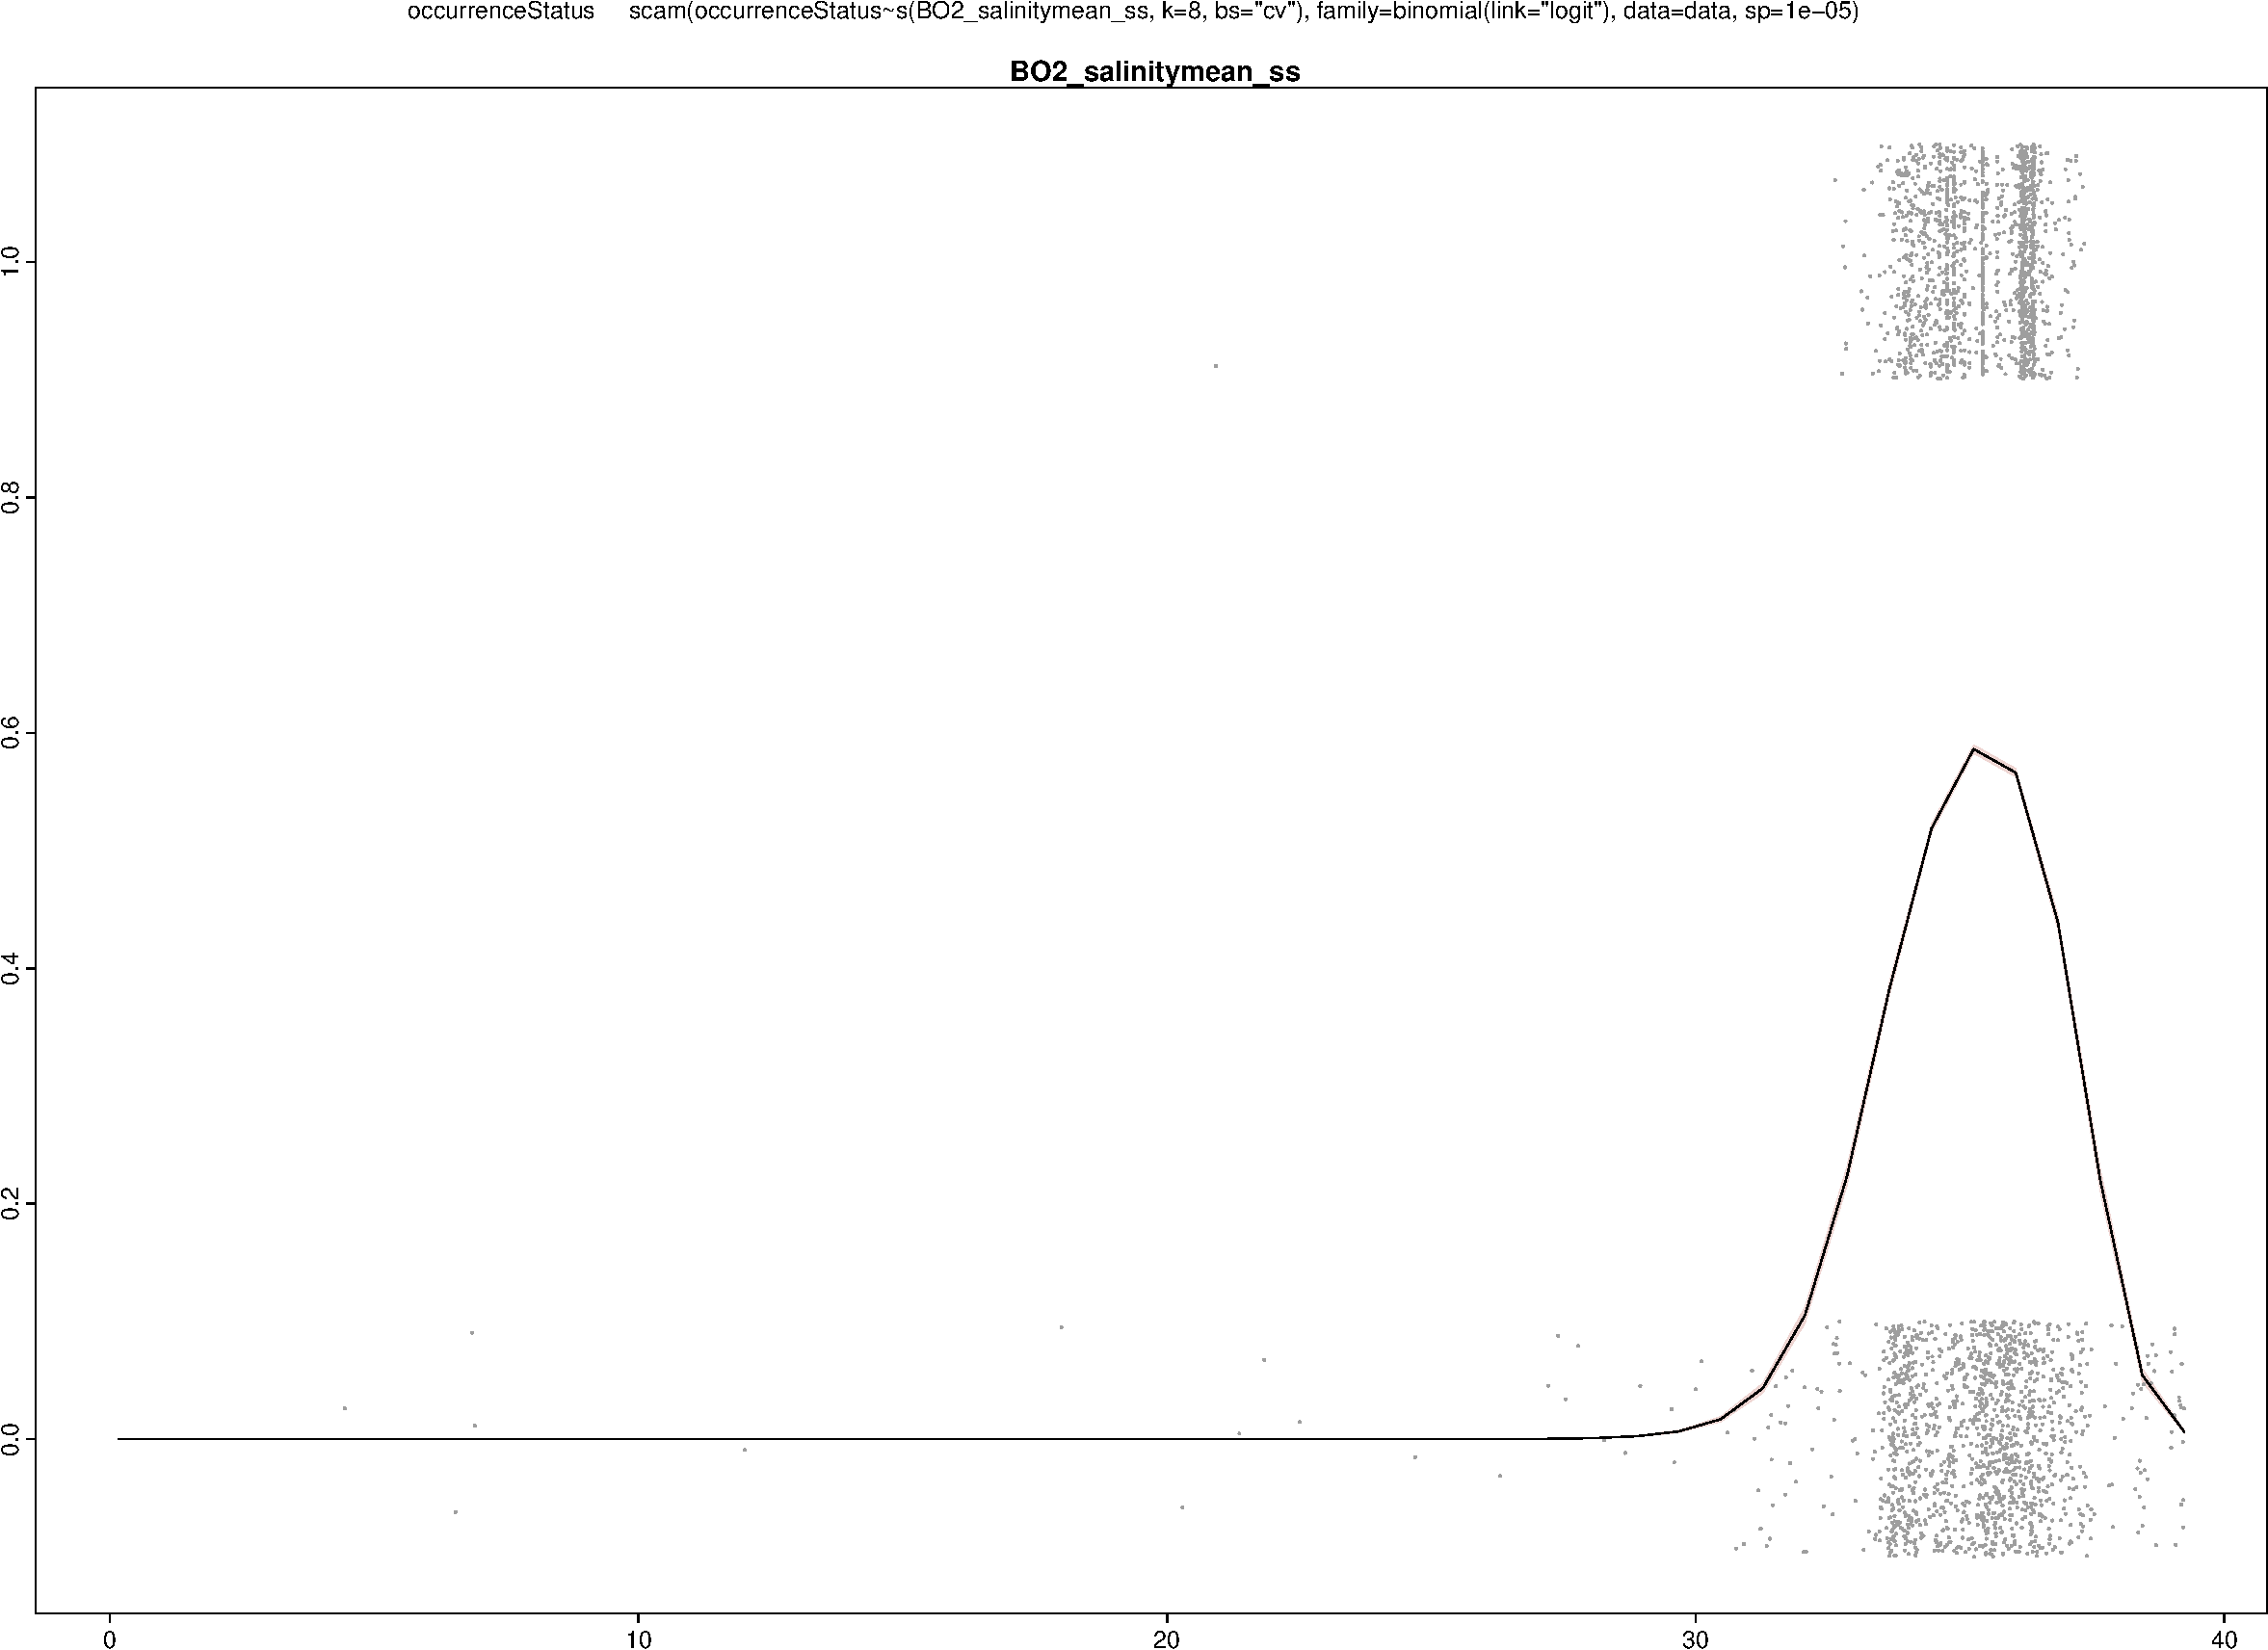
\includegraphics{_main_files/figure-latex/unnamed-chunk-63-1.pdf}

We can see in the summary of the fit, that all included variables are statistically significant (with p\textless0.05) and present a unimodal response curve.

For a more detailed check of the fitting, we can use the scam.check function:

\begin{Shaded}
\begin{Highlighting}[]
\FunctionTok{scam.check}\NormalTok{(model)}
\end{Highlighting}
\end{Shaded}

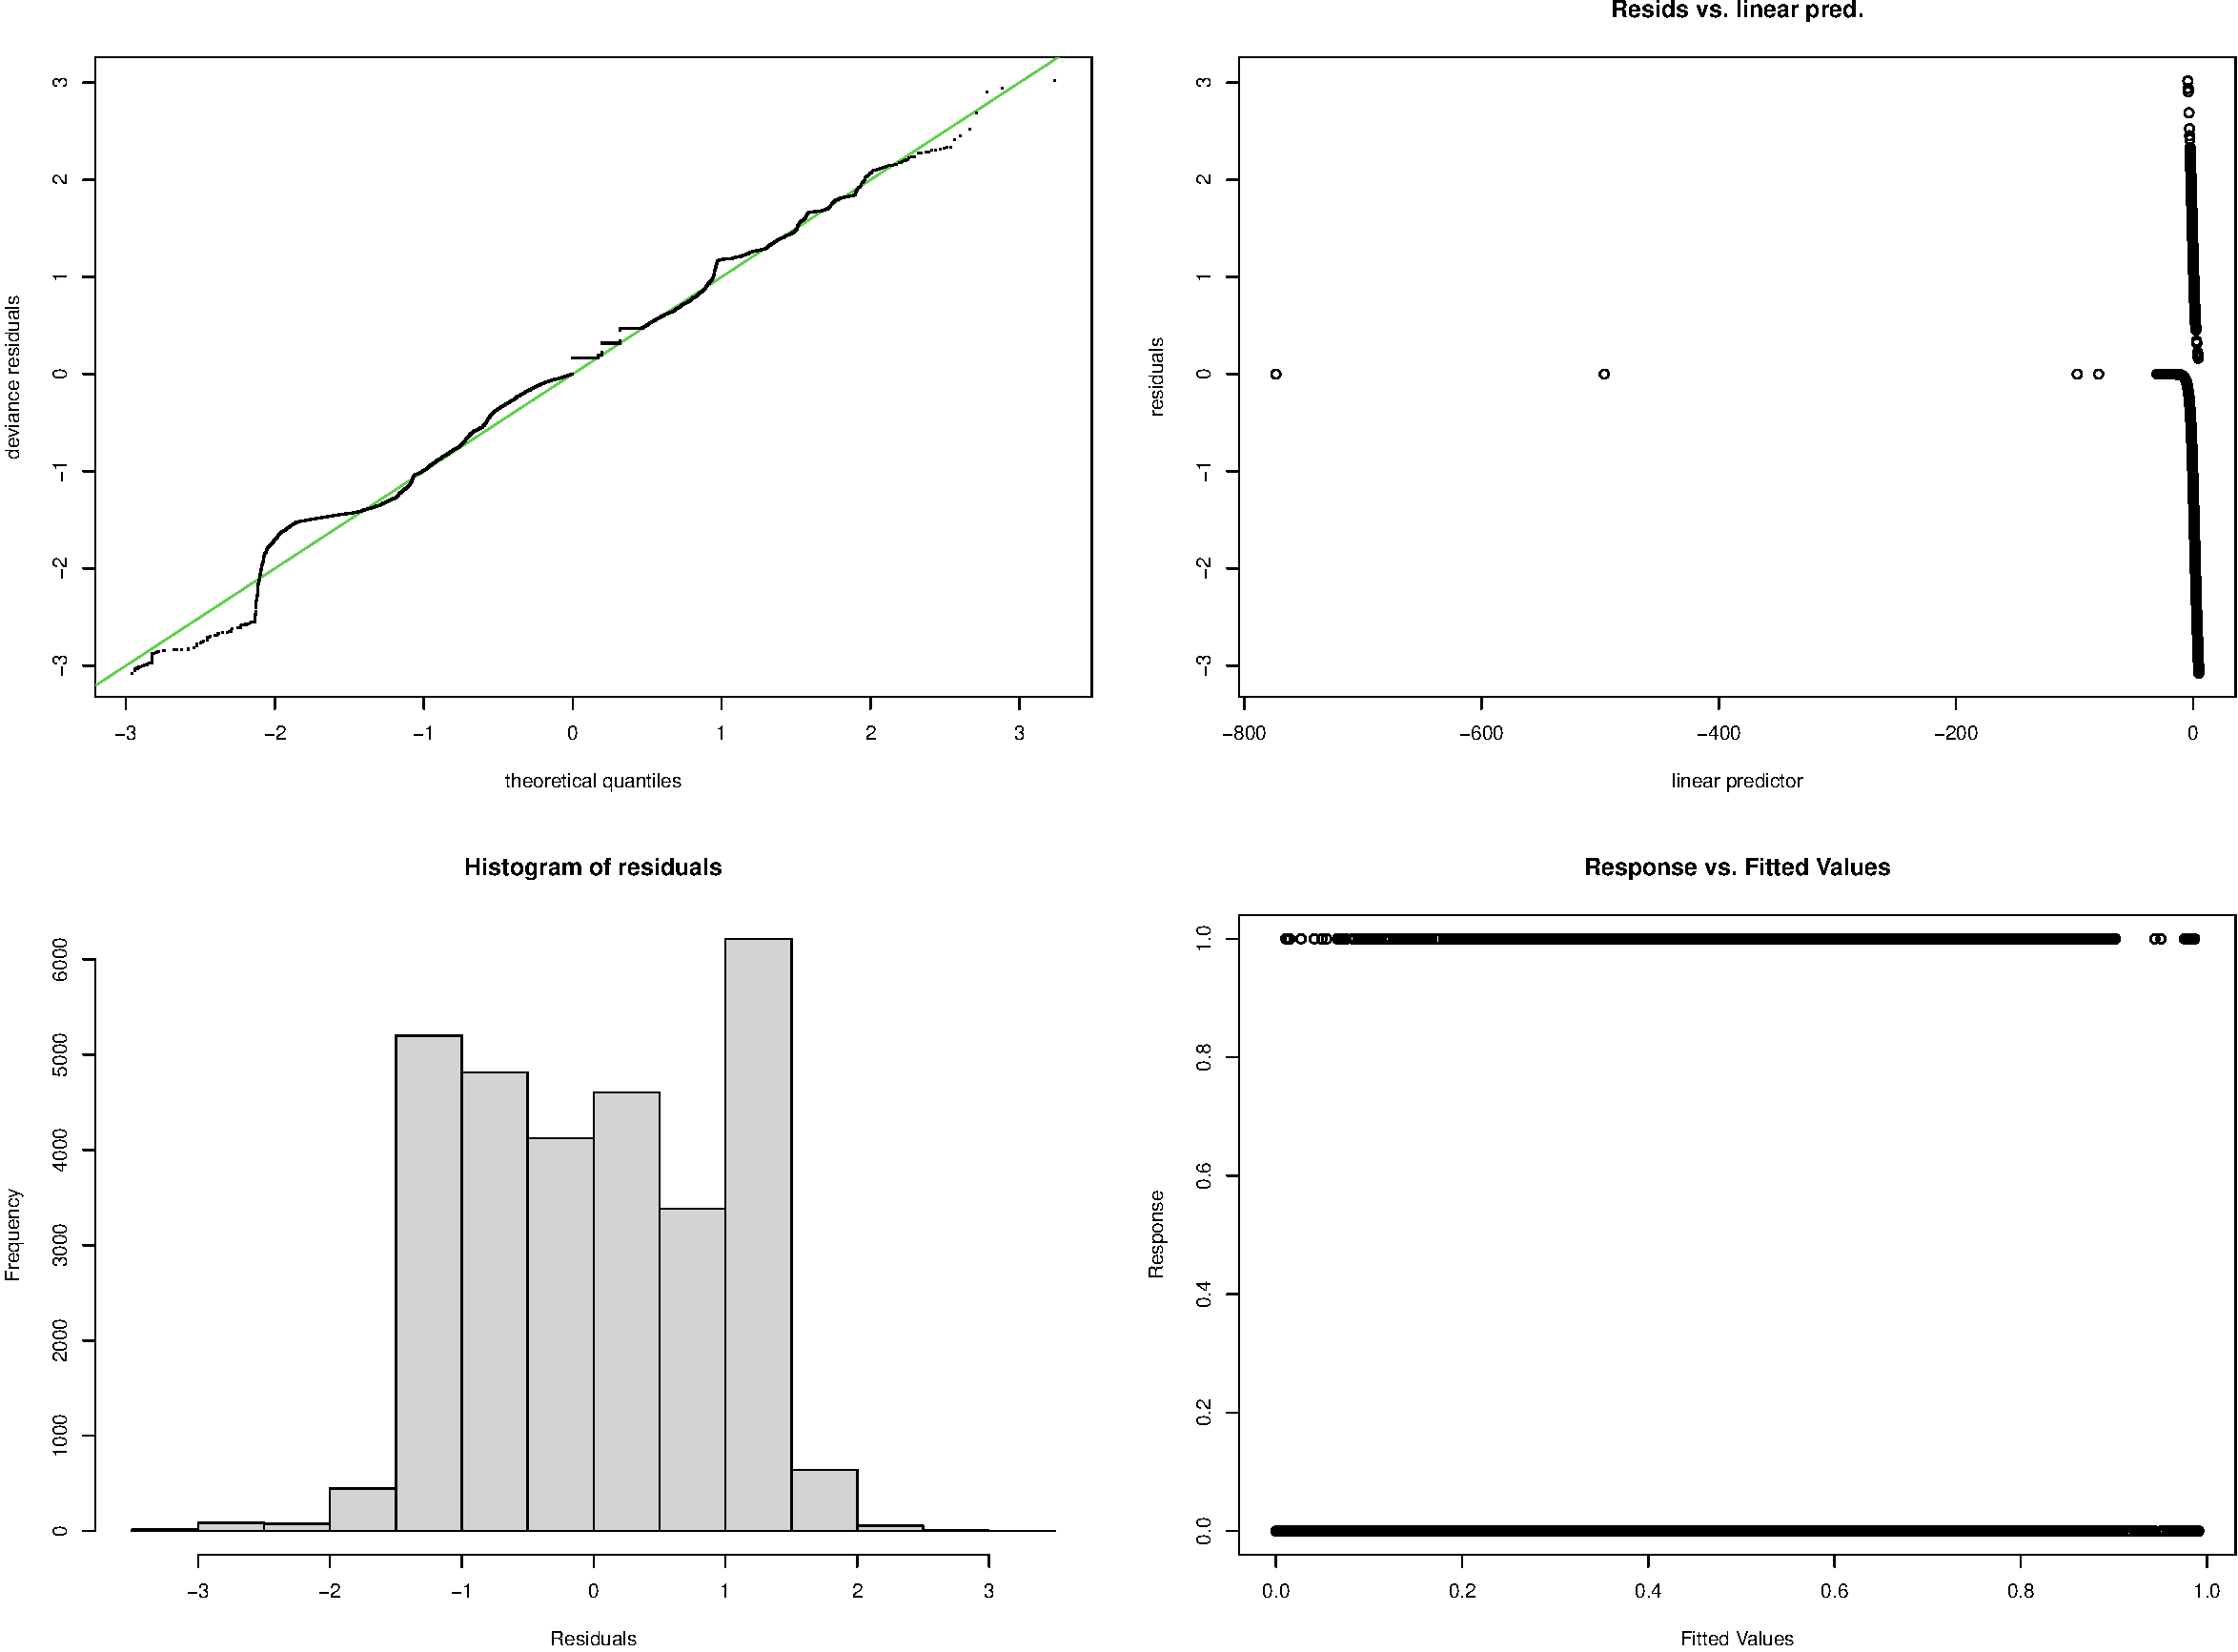
\includegraphics{_main_files/figure-latex/unnamed-chunk-64-1.pdf}

\begin{verbatim}
## 
## Method: UBRE   Optimizer: NA newton
## The optimal smoothing parameter(s): 1e-05 1e-05 1e-05 .
\end{verbatim}

\hypertarget{model-selection}{%
\section{Model selection}\label{model-selection}}

When several explanatory variables are available, a variable selection process can be carried out. Here we provide as an example, a function that performs forward variable selection (modsel.scam) based on the significance of variables and AIC values of the fits.

\begin{Shaded}
\begin{Highlighting}[]
\FunctionTok{source}\NormalTok{(}\StringTok{"function/function\_scam\_selection\_optimized.R"}\NormalTok{)}
\end{Highlighting}
\end{Shaded}

We save the names of the variables we want to introduce for the variable selection process as a vector:

\begin{Shaded}
\begin{Highlighting}[]
\NormalTok{vars }\OtherTok{\textless{}{-}} \FunctionTok{c}\NormalTok{(}\StringTok{"BO\_sstmean"}\NormalTok{,}
          \StringTok{"BO2\_salinitymean\_ss"}\NormalTok{,}
          \StringTok{"BO2\_chlomean\_ss"}\NormalTok{)}
\end{Highlighting}
\end{Shaded}

The default AIC tolerance is 2 and there is not a limit on selected terms in this example. These options can be modified through aic.tol and vmax arguments in the function. The number of knots and the sp can be also modified.

\begin{Shaded}
\begin{Highlighting}[]
\NormalTok{model\_SCGAM }\OtherTok{\textless{}{-}} \FunctionTok{try}\NormalTok{(}\FunctionTok{modsel.scam}\NormalTok{(}\AttributeTok{basef=}\StringTok{"occurrenceStatus \textasciitilde{} 1"}\NormalTok{, }\AttributeTok{vars=}\NormalTok{vars, }\AttributeTok{dat=}\NormalTok{data,}\AttributeTok{sp=}\FloatTok{0.00001}\NormalTok{), }\AttributeTok{silent=}\NormalTok{T)  }
\end{Highlighting}
\end{Shaded}

\begin{verbatim}
## [1] "Fitting models with 1 terms"
##   occurrenceStatus ~ 1+s(BO_sstmean,m=2,bs='cv',k=8) 
##   occurrenceStatus ~ 1+s(BO2_salinitymean_ss,m=2,bs='cv',k=8) 
##   occurrenceStatus ~ 1+s(BO2_chlomean_ss,m=2,bs='cv',k=8) 
## [1] "Fitting models with 2 terms"
##   occurrenceStatus ~ 1+s(BO_sstmean,m=2,bs='cv',k=8)+s(BO2_salinitymean_ss,m=2,bs='cv',k=8) 
##   occurrenceStatus ~ 1+s(BO_sstmean,m=2,bs='cv',k=8)+s(BO2_chlomean_ss,m=2,bs='cv',k=8) 
## [1] "Fitting models with 3 terms"
##   occurrenceStatus ~ 1+s(BO_sstmean,m=2,bs='cv',k=8)+s(BO2_chlomean_ss,m=2,bs='cv',k=8)+s(BO2_salinitymean_ss,m=2,bs='cv',k=8)
\end{verbatim}

We check results of the selected model, such as, selected variable names:

\begin{Shaded}
\begin{Highlighting}[]
\NormalTok{model\_SCGAM}\SpecialCharTok{$}\NormalTok{svars}
\end{Highlighting}
\end{Shaded}

\begin{verbatim}
## [1] "BO_sstmean"          "BO2_chlomean_ss"     "BO2_salinitymean_ss"
\end{verbatim}

AICs of the fitted models:

\begin{Shaded}
\begin{Highlighting}[]
\FunctionTok{sapply}\NormalTok{(model\_SCGAM}\SpecialCharTok{$}\NormalTok{smod, AIC)}
\end{Highlighting}
\end{Shaded}

\begin{verbatim}
##                null          BO_sstmean     BO2_chlomean_ss BO2_salinitymean_ss 
##            41120.17            31629.43            28388.33            28032.06
\end{verbatim}

Explained deviance of fitted models:

\begin{Shaded}
\begin{Highlighting}[]
\FunctionTok{sapply}\NormalTok{(model\_SCGAM}\SpecialCharTok{$}\NormalTok{smod, }\ControlFlowTok{function}\NormalTok{(x) }\FunctionTok{summary}\NormalTok{(x)}\SpecialCharTok{$}\NormalTok{dev.expl)}
\end{Highlighting}
\end{Shaded}

\begin{verbatim}
##                null          BO_sstmean     BO2_chlomean_ss BO2_salinitymean_ss 
##        3.539048e-16        2.309134e-01        3.100285e-01        3.187874e-01
\end{verbatim}

Formulas of the fitted models:

\begin{Shaded}
\begin{Highlighting}[]
\FunctionTok{lapply}\NormalTok{(model\_SCGAM}\SpecialCharTok{$}\NormalTok{smod, formula)}
\end{Highlighting}
\end{Shaded}

\begin{verbatim}
## $null
## occurrenceStatus ~ 1
## <environment: 0x000002667cc23298>
## 
## $BO_sstmean
## occurrenceStatus ~ 1 + s(BO_sstmean, m = 2, bs = "cv", k = 8)
## <environment: 0x000002667cc23298>
## 
## $BO2_chlomean_ss
## occurrenceStatus ~ 1 + s(BO_sstmean, m = 2, bs = "cv", k = 8) + 
##     s(BO2_chlomean_ss, m = 2, bs = "cv", k = 8)
## <environment: 0x000002667cc23298>
## 
## $BO2_salinitymean_ss
## occurrenceStatus ~ 1 + s(BO_sstmean, m = 2, bs = "cv", k = 8) + 
##     s(BO2_chlomean_ss, m = 2, bs = "cv", k = 8) + s(BO2_salinitymean_ss, 
##     m = 2, bs = "cv", k = 8)
## <environment: 0x000002667cc23298>
\end{verbatim}

Summaries of the fitted models:

\begin{Shaded}
\begin{Highlighting}[]
\FunctionTok{lapply}\NormalTok{(model\_SCGAM}\SpecialCharTok{$}\NormalTok{smod, summary)}
\end{Highlighting}
\end{Shaded}

\begin{verbatim}
## $null
## 
## Family: binomial 
## Link function: logit 
## 
## Formula:
## occurrenceStatus ~ 1
## <environment: 0x000002667cc23298>
## 
## Parametric coefficients:
##             Estimate Std. Error z value Pr(>|z|)
## (Intercept) 0.009777   0.011613   0.842      0.4
## 
## 
## R-sq.(adj) =      0   Deviance explained = 3.54e-14%
##   Scale est. = 1         n = 29661
## 
## 
## $BO_sstmean
## 
## Family: binomial 
## Link function: logit 
## 
## Formula:
## occurrenceStatus ~ 1 + s(BO_sstmean, m = 2, bs = "cv", k = 8)
## <environment: 0x000002667cc23298>
## 
## Parametric coefficients:
##             Estimate Std. Error z value Pr(>|z|)    
## (Intercept)   -47.30       3.12  -15.16   <2e-16 ***
## ---
## Signif. codes:  0 '***' 0.001 '**' 0.01 '*' 0.05 '.' 0.1 ' ' 1
## 
## Approximate significance of smooth terms:
##               edf Ref.df Chi.sq p-value    
## s(BO_sstmean)   2      2  987.3  <2e-16 ***
## ---
## Signif. codes:  0 '***' 0.001 '**' 0.01 '*' 0.05 '.' 0.1 ' ' 1
## 
## R-sq.(adj) =  0.2607   Deviance explained = 23.1%
##   Scale est. = 1         n = 29661
## 
## 
## $BO2_chlomean_ss
## 
## Family: binomial 
## Link function: logit 
## 
## Formula:
## occurrenceStatus ~ 1 + s(BO_sstmean, m = 2, bs = "cv", k = 8) + 
##     s(BO2_chlomean_ss, m = 2, bs = "cv", k = 8)
## <environment: 0x000002667cc23298>
## 
## Parametric coefficients:
##             Estimate Std. Error z value Pr(>|z|)
## (Intercept)   -40.38      89.57  -0.451    0.652
## 
## Approximate significance of smooth terms:
##                      edf Ref.df Chi.sq p-value    
## s(BO_sstmean)      3.978  4.004  938.3  <2e-16 ***
## s(BO2_chlomean_ss) 4.002  4.005 2374.3  <2e-16 ***
## ---
## Signif. codes:  0 '***' 0.001 '**' 0.01 '*' 0.05 '.' 0.1 ' ' 1
## 
## R-sq.(adj) =  0.3399   Deviance explained =   31%
##   Scale est. = 1         n = 29661
## 
## 
## $BO2_salinitymean_ss
## 
## Family: binomial 
## Link function: logit 
## 
## Formula:
## occurrenceStatus ~ 1 + s(BO_sstmean, m = 2, bs = "cv", k = 8) + 
##     s(BO2_chlomean_ss, m = 2, bs = "cv", k = 8) + s(BO2_salinitymean_ss, 
##     m = 2, bs = "cv", k = 8)
## <environment: 0x000002667cc23298>
## 
## Parametric coefficients:
##             Estimate Std. Error z value Pr(>|z|)
## (Intercept)   -56.08      45.69  -1.227     0.22
## 
## Approximate significance of smooth terms:
##                          edf Ref.df Chi.sq p-value    
## s(BO_sstmean)          3.936  3.999  772.6  <2e-16 ***
## s(BO2_chlomean_ss)     3.985  4.003 1820.7  <2e-16 ***
## s(BO2_salinitymean_ss) 2.001  2.001  191.4  <2e-16 ***
## ---
## Signif. codes:  0 '***' 0.001 '**' 0.01 '*' 0.05 '.' 0.1 ' ' 1
## 
## R-sq.(adj) =  0.3488   Deviance explained = 31.9%
##   Scale est. = 1         n = 29661
\end{verbatim}

The last model of the list, is the selected one. Which in this case contains the considered three variables.

\begin{Shaded}
\begin{Highlighting}[]
\NormalTok{selected\_model }\OtherTok{\textless{}{-}}\NormalTok{ model\_SCGAM}\SpecialCharTok{$}\NormalTok{smod[[}\FunctionTok{length}\NormalTok{(model\_SCGAM}\SpecialCharTok{$}\NormalTok{smod)]]}
\end{Highlighting}
\end{Shaded}

We save the selected model

\begin{Shaded}
\begin{Highlighting}[]
\FunctionTok{save}\NormalTok{(}\AttributeTok{list=}\StringTok{"selected\_model"}\NormalTok{, }\AttributeTok{file=}\StringTok{"models/selected\_model.RData"}\NormalTok{)}
\end{Highlighting}
\end{Shaded}

Note that there are multiple options and criteria for model selection that are not reviewed here. Any model selection technique used for GAMs can be used also for SC-GAMs.

\hypertarget{model-validation}{%
\chapter{Model validation}\label{model-validation}}

In this section, model validation is performed in order to assess the predictive performance of the selected model. This validation is conducted via k-fold cross-validation. The data set is divided into k equally sized groups \citep{hijmans_2012}, using a percentage of randomly selected observations to run the model and the remaining for validation, iteratively for each fold.

First we load the list of required libraries.

\begin{Shaded}
\begin{Highlighting}[]
\NormalTok{requiredPackages }\OtherTok{\textless{}{-}} \FunctionTok{c}\NormalTok{(}
  \CommentTok{\#GENERAL USE LIBRARIES {-}{-}{-}{-}{-}{-}{-}{-}\#}
  \StringTok{"here"}\NormalTok{, }\CommentTok{\# Library for reproducible workflow}
  \StringTok{"rstudioapi"}\NormalTok{,  }\CommentTok{\# Library for reproducible workflow}
  \StringTok{"stringr"}\NormalTok{,}
  \StringTok{"RColorBrewer"}\NormalTok{,  }
  \StringTok{"ggplot2"}\NormalTok{,}
  \StringTok{"dplyr"}\NormalTok{,}
  \StringTok{"tidyverse"}\NormalTok{,}
  \StringTok{"R.utils"}\NormalTok{,}
  \StringTok{"ggpubr"}\NormalTok{,}
  \StringTok{"hrbrthemes"}\NormalTok{,}
  
  \CommentTok{\#SPATIAL DATA {-}{-}{-}{-}{-}{-}{-}{-}\#}
  \StringTok{"rgdal"}\NormalTok{,}
  \StringTok{"fields"}\NormalTok{,}
  \StringTok{"maps"}\NormalTok{ ,}
  \StringTok{"raster"}\NormalTok{,}

  \CommentTok{\#MODEL FIT {-}{-}{-}{-}{-}{-}{-}{-}\#}
  \StringTok{"scam"}\NormalTok{,}
  \StringTok{"plotmo"}\NormalTok{,}
  \StringTok{"SDMTools"}\NormalTok{,}
  \StringTok{"pkgbuild"}\NormalTok{,}
  \StringTok{"dismo"}
\NormalTok{  )}
\end{Highlighting}
\end{Shaded}

We run a function to install the required packages that are not in our system and load all the required packages.

\begin{Shaded}
\begin{Highlighting}[]
\NormalTok{install\_load\_function }\OtherTok{\textless{}{-}} \ControlFlowTok{function}\NormalTok{(pkg)\{}
\NormalTok{  new.pkg }\OtherTok{\textless{}{-}}\NormalTok{ pkg[}\SpecialCharTok{!}\NormalTok{(pkg }\SpecialCharTok{\%in\%} \FunctionTok{installed.packages}\NormalTok{()[, }\StringTok{"Package"}\NormalTok{])]}
  \ControlFlowTok{if}\NormalTok{ (}\FunctionTok{length}\NormalTok{(new.pkg))}
    \FunctionTok{install.packages}\NormalTok{(new.pkg, }\AttributeTok{dependencies =} \ConstantTok{TRUE}\NormalTok{)}
  \FunctionTok{sapply}\NormalTok{(pkg, require, }\AttributeTok{character.only =} \ConstantTok{TRUE}\NormalTok{)}
\NormalTok{\}}

\FunctionTok{install\_load\_function}\NormalTok{(requiredPackages)}
\end{Highlighting}
\end{Shaded}

\begin{verbatim}
##         here   rstudioapi      stringr RColorBrewer      ggplot2        dplyr 
##         TRUE         TRUE         TRUE         TRUE         TRUE         TRUE 
##    tidyverse      R.utils       ggpubr   hrbrthemes        rgdal       fields 
##         TRUE         TRUE         TRUE         TRUE         TRUE         TRUE 
##         maps       raster         scam       plotmo     SDMTools     pkgbuild 
##         TRUE         TRUE         TRUE         TRUE         TRUE         TRUE 
##        dismo 
##         TRUE
\end{verbatim}

We define some overall settings.

\begin{Shaded}
\begin{Highlighting}[]
\CommentTok{\# General settings for ggplot (black{-}white background, larger base\_size)}
\FunctionTok{theme\_set}\NormalTok{(}\FunctionTok{theme\_bw}\NormalTok{(}\AttributeTok{base\_size =} \DecValTok{16}\NormalTok{))}
\end{Highlighting}
\end{Shaded}

We load output from the selected model saved in the previous step.

\begin{Shaded}
\begin{Highlighting}[]
\FunctionTok{load}\NormalTok{(here}\SpecialCharTok{::}\FunctionTok{here}\NormalTok{ (}\StringTok{"models"}\NormalTok{, }\StringTok{"selected\_model.Rdata"}\NormalTok{))}
\end{Highlighting}
\end{Shaded}

\hypertarget{optimum-threshold}{%
\section{Optimum threshold}\label{optimum-threshold}}

We generate a data frame with the data used in the selected model and we add the predicted values.

\begin{Shaded}
\begin{Highlighting}[]
  \CommentTok{\#PAdata\_enviroment used in the selected model}
\NormalTok{  data}\OtherTok{\textless{}{-}}\NormalTok{selected\_model}\SpecialCharTok{$}\NormalTok{model}

  \CommentTok{\# Predict }
\NormalTok{  scgam.pred }\OtherTok{\textless{}{-}} \FunctionTok{predict}\NormalTok{(selected\_model, }\AttributeTok{newdata=}\NormalTok{data, }\AttributeTok{type=}\StringTok{"response"}\NormalTok{)}
  
  \CommentTok{\# Add the prediction to the data object}
\NormalTok{  data}\SpecialCharTok{$}\NormalTok{scgam.pred }\OtherTok{\textless{}{-}} \FunctionTok{as.vector}\NormalTok{(scgam.pred)}
  \FunctionTok{head}\NormalTok{(data)}
\end{Highlighting}
\end{Shaded}

\begin{verbatim}
##    occurrenceStatus BO_sstmean BO2_chlomean_ss BO2_salinitymean_ss scgam.pred
## 1                 1   16.99439      1.20410309            35.42666  0.9804524
## 5                 1   16.99439      1.20410309            35.42666  0.9804524
## 8                 1   25.52963      0.08455528            36.43070  0.4238477
## 10                1   16.99439      1.20410309            35.42666  0.9804524
## 11                1   15.21486      0.72283228            34.20426  0.8449155
## 12                1   16.99439      1.20410309            35.42666  0.9804524
\end{verbatim}

The threshold for presence-absence classification for each species is obtained as the values maximizing sensitivity plus specificity \citep{jimenez_etal_2007}. If the result was a range (instead of a single value), we would select the mean value of the range.

\begin{Shaded}
\begin{Highlighting}[]
  \CommentTok{\# Optimizing the threshold probability}
\NormalTok{  obs }\OtherTok{\textless{}{-}}\NormalTok{ data}\SpecialCharTok{$}\NormalTok{occurrenceStatus}
\NormalTok{  predSCGAM\_P }\OtherTok{\textless{}{-}}\NormalTok{ data}\SpecialCharTok{$}\NormalTok{scgam.pred}
  
  \CommentTok{\# threshold optimizing}
\NormalTok{  myoptim }\OtherTok{\textless{}{-}} \FunctionTok{optim.thresh}\NormalTok{ (obs,predSCGAM\_P)}
\NormalTok{  myoptim}
\end{Highlighting}
\end{Shaded}

\begin{verbatim}
## $min.occurence.prediction
## [1] 0.01156124
## 
## $mean.occurence.prediction
## [1] 0.6642745
## 
## $`10.percent.omission`
## [1] 0.36
## 
## $`sensitivity=specificity`
## [1] 0.44
## 
## $`max.sensitivity+specificity`
## [1] 0.42
## 
## $maxKappa
## [1] 0.42
## 
## $max.prop.correct
## [1] 0.42
## 
## $min.ROC.plot.distance
## [1] 0.42
\end{verbatim}

\begin{Shaded}
\begin{Highlighting}[]
  \CommentTok{\# select the threshold that maximizes the sum of sensitivity and specificity }
\NormalTok{  myThreshold }\OtherTok{\textless{}{-}} \FunctionTok{as.numeric}\NormalTok{((myoptim[[}\StringTok{"max.sensitivity+specificity"}\NormalTok{]]))}
\end{Highlighting}
\end{Shaded}

Accuracy indicators, such as AUC (Area Under the Receiver Operating Characteristic---ROC---curve), sensitivity (true predicted presences) and specificity (true predicted absences) are first computed for the all observations.

\begin{Shaded}
\begin{Highlighting}[]
  \CommentTok{\# Accuracy values with all observations}
  \FunctionTok{accuracy}\NormalTok{ (obs, predSCGAM\_P, }\AttributeTok{threshold=}\NormalTok{myThreshold)}
\end{Highlighting}
\end{Shaded}

\begin{verbatim}
##   threshold       AUC omission.rate sensitivity specificity prop.correct
## 1      0.42 0.7415229     0.1985506   0.8014494   0.6815964    0.7418159
##      Kappa
## 1 0.483323
\end{verbatim}

\begin{Shaded}
\begin{Highlighting}[]
  \CommentTok{\# Create confusion matrix with all observations}
  \FunctionTok{confusion.matrix}\NormalTok{(obs, predSCGAM\_P, }\AttributeTok{threshold=}\NormalTok{myThreshold)}
\end{Highlighting}
\end{Shaded}

\begin{verbatim}
##     obs
## pred     0     1
##    0 10059  2959
##    1  4699 11944
## attr(,"class")
## [1] "confusion.matrix"
\end{verbatim}

\hypertarget{k-fold-validation}{%
\section{k-fold validation}\label{k-fold-validation}}

In this case we use a 5-fold cross-validation.

\begin{Shaded}
\begin{Highlighting}[]
  \CommentTok{\# Number of groups}
\NormalTok{  k }\OtherTok{\textless{}{-}} \DecValTok{5} 
  \CommentTok{\# Generate groups}
\NormalTok{  groups}\OtherTok{\textless{}{-}}\FunctionTok{kfold}\NormalTok{(data, k, }\AttributeTok{by=}\NormalTok{data}\SpecialCharTok{$}\NormalTok{occurrencestatus)}
\end{Highlighting}
\end{Shaded}

The model is run for each of the 5 random subset (with a 20\% of the observations) and indicators are then computed using the remaining 80\% of the observations. Indicators are the averaged across folds.

\begin{Shaded}
\begin{Highlighting}[]
  \CommentTok{\# Initialise the confusion matrix and the accuracy table: }
\NormalTok{  myCM }\OtherTok{\textless{}{-}} \ConstantTok{NULL} 
\NormalTok{  myACC }\OtherTok{\textless{}{-}} \ConstantTok{NULL}
  
  \CommentTok{\# get the formula of the selected model  }
\NormalTok{  formula }\OtherTok{\textless{}{-}} \FunctionTok{summary}\NormalTok{(selected\_model)[[}\StringTok{"formula"}\NormalTok{]]}
  
  \CommentTok{\# get the smoothing parameters of the selected model  }
\NormalTok{  sp }\OtherTok{\textless{}{-}}\NormalTok{ selected\_model}\SpecialCharTok{$}\NormalTok{sp}

  \CommentTok{\# loop for each group k}
  \ControlFlowTok{for}\NormalTok{ (j }\ControlFlowTok{in} \DecValTok{1}\SpecialCharTok{:}\NormalTok{k) \{}
    \CommentTok{\# Preparation of Training Sites}
\NormalTok{    p\_Training }\OtherTok{\textless{}{-}}\NormalTok{ data[groups }\SpecialCharTok{!=}\NormalTok{ j,]}
    
    \CommentTok{\# Model fit}
\NormalTok{    selected\_model.sp.j }\OtherTok{\textless{}{-}} \FunctionTok{scam}\NormalTok{ (formula, }\AttributeTok{family=}\FunctionTok{binomial}\NormalTok{(}\AttributeTok{link=}\StringTok{"logit"}\NormalTok{),}\AttributeTok{data=}\NormalTok{p\_Training, }\AttributeTok{sp=}\FunctionTok{c}\NormalTok{(sp))}
    
    \CommentTok{\# Predict Model}
\NormalTok{    p\_validacion}\OtherTok{\textless{}{-}}\NormalTok{data[groups }\SpecialCharTok{==}\NormalTok{ j,]}
    
\NormalTok{    selected\_model.sp.j.pred }\OtherTok{\textless{}{-}} \FunctionTok{predict}\NormalTok{(selected\_model.sp.j, }\AttributeTok{newdata=}\NormalTok{p\_validacion, }\AttributeTok{type=}\StringTok{"response"}\NormalTok{)}
\NormalTok{    p\_validacion}\SpecialCharTok{$}\NormalTok{Pred }\OtherTok{\textless{}{-}}\NormalTok{ selected\_model.sp.j.pred}
    
    \CommentTok{\# Confussion matrix and accuracy table for fold j}
\NormalTok{    obs }\OtherTok{\textless{}{-}}\NormalTok{ p\_validacion}\SpecialCharTok{$}\NormalTok{occurrenceStatus}
\NormalTok{    predSCGAM }\OtherTok{\textless{}{-}}\NormalTok{ p\_validacion}\SpecialCharTok{$}\NormalTok{Pred}
\NormalTok{    myCM }\OtherTok{\textless{}{-}} \FunctionTok{rbind}\NormalTok{(myCM, }\FunctionTok{as.numeric}\NormalTok{(}\FunctionTok{confusion.matrix}\NormalTok{(obs, predSCGAM, }\AttributeTok{threshold=}\NormalTok{myThreshold)))}
\NormalTok{    myACC }\OtherTok{\textless{}{-}} \FunctionTok{rbind}\NormalTok{(myACC, }\FunctionTok{accuracy}\NormalTok{(obs, predSCGAM, }\AttributeTok{threshold=}\NormalTok{myThreshold))}
\NormalTok{  \} }
  
  \CommentTok{\# Mean values across k{-}folds}
\NormalTok{  validation\_summary}\OtherTok{\textless{}{-}}\FunctionTok{cbind}\NormalTok{(}\AttributeTok{Threshold=}\NormalTok{myThreshold,}
                            \AttributeTok{mean\_AUC=}\FunctionTok{mean}\NormalTok{(myACC}\SpecialCharTok{$}\NormalTok{AUC),}
                            \AttributeTok{mean\_Omision=}\FunctionTok{mean}\NormalTok{(myACC}\SpecialCharTok{$}\NormalTok{omission.rate),}
                            \AttributeTok{mean\_sensitivity=}\FunctionTok{mean}\NormalTok{(myACC}\SpecialCharTok{$}\NormalTok{sensitivity),}
                            \AttributeTok{mean\_specificity=}\FunctionTok{mean}\NormalTok{(myACC}\SpecialCharTok{$}\NormalTok{specificity),}
                            \AttributeTok{mean\_Prop.Corr=}\FunctionTok{mean}\NormalTok{(myACC}\SpecialCharTok{$}\NormalTok{prop.correct))}

\NormalTok{  validation\_summary}
\end{Highlighting}
\end{Shaded}

\begin{verbatim}
##      Threshold mean_AUC mean_Omision mean_sensitivity mean_specificity
## [1,]      0.42 0.725464    0.2399716        0.7600284        0.6908995
##      mean_Prop.Corr
## [1,]      0.7256674
\end{verbatim}

We save the validation summary object.

\begin{Shaded}
\begin{Highlighting}[]
\FunctionTok{save}\NormalTok{(validation\_summary, }\AttributeTok{file =}\NormalTok{ here}\SpecialCharTok{::}\FunctionTok{here}\NormalTok{(}\StringTok{"models/validation\_summary.RData"}\NormalTok{))}
\end{Highlighting}
\end{Shaded}

\hypertarget{prediction-and-maps}{%
\chapter{Prediction and maps}\label{prediction-and-maps}}

In this chapter we predict from the fitted model and produce final SDMs maps.

First we load a list of required libraries.

\begin{Shaded}
\begin{Highlighting}[]
\NormalTok{requiredPackages }\OtherTok{\textless{}{-}} \FunctionTok{c}\NormalTok{(}
  \CommentTok{\#GENERAL USE LIBRARIES {-}{-}{-}{-}{-}{-}{-}{-}\#}
  \StringTok{"here"}\NormalTok{, }\CommentTok{\# Library for reproducible workflow}
  \StringTok{"rstudioapi"}\NormalTok{,  }\CommentTok{\# Library for reproducible workflow}
  \StringTok{"ggplot2"}\NormalTok{, }\CommentTok{\#for plotting}
  \StringTok{"tidyverse"}\NormalTok{, }
  \StringTok{"rgdal"}\NormalTok{, }\CommentTok{\# to work with Spatial data}
  \StringTok{"raster"}\NormalTok{, }\CommentTok{\#spatial }
  \StringTok{"maps"}\NormalTok{, }\CommentTok{\#world map}
  \StringTok{"maptools"}\NormalTok{, }\CommentTok{\#plotting world map}
  \StringTok{"RColorBrewer"}\NormalTok{, }\CommentTok{\#color palette}
  \StringTok{"scam"}\NormalTok{, }\CommentTok{\#sdm models under the ecological niche theory framework}
  \StringTok{"ggpubr"}
\NormalTok{  )}
\end{Highlighting}
\end{Shaded}

We run a function to install the required packages that are not in our system and load all the required packages.

\begin{Shaded}
\begin{Highlighting}[]
\NormalTok{install\_load\_function }\OtherTok{\textless{}{-}} \ControlFlowTok{function}\NormalTok{(pkg)\{}
\NormalTok{  new.pkg }\OtherTok{\textless{}{-}}\NormalTok{ pkg[}\SpecialCharTok{!}\NormalTok{(pkg }\SpecialCharTok{\%in\%} \FunctionTok{installed.packages}\NormalTok{()[, }\StringTok{"Package"}\NormalTok{])]}
  \ControlFlowTok{if}\NormalTok{ (}\FunctionTok{length}\NormalTok{(new.pkg))}
    \FunctionTok{install.packages}\NormalTok{(new.pkg, }\AttributeTok{dependencies =} \ConstantTok{TRUE}\NormalTok{)}
  \FunctionTok{sapply}\NormalTok{(pkg, require, }\AttributeTok{character.only =} \ConstantTok{TRUE}\NormalTok{)}
\NormalTok{\}}

\FunctionTok{install\_load\_function}\NormalTok{(requiredPackages)}
\end{Highlighting}
\end{Shaded}

\begin{verbatim}
##         here   rstudioapi      ggplot2    tidyverse        rgdal       raster 
##         TRUE         TRUE         TRUE         TRUE         TRUE         TRUE 
##         maps     maptools RColorBrewer         scam       ggpubr 
##         TRUE         TRUE         TRUE         TRUE         TRUE
\end{verbatim}

We define some overall settings.

\begin{Shaded}
\begin{Highlighting}[]
\CommentTok{\# General settings for ggplot (black{-}white background, larger base\_size)}
\FunctionTok{theme\_set}\NormalTok{(}\FunctionTok{theme\_bw}\NormalTok{(}\AttributeTok{base\_size =} \DecValTok{16}\NormalTok{))}
\end{Highlighting}
\end{Shaded}

\hypertarget{prepare-environmental-data.}{%
\section{Prepare environmental data.}\label{prepare-environmental-data.}}

In previous steps (see Chapter 2), we have defined the study area that defines the extent of our spatial data. We load the \texttt{study\_area} object that is a SpatialPolygonsDataFrame class:

\begin{Shaded}
\begin{Highlighting}[]
\FunctionTok{load}\NormalTok{(here}\SpecialCharTok{::}\FunctionTok{here}\NormalTok{ (}\StringTok{"data"}\NormalTok{, }\StringTok{"spatial"}\NormalTok{, }\StringTok{"study\_area.RData"}\NormalTok{))}
\end{Highlighting}
\end{Shaded}

And we load the rasterStack with the downloaded environmental data.

\begin{Shaded}
\begin{Highlighting}[]
\NormalTok{mylayers}\OtherTok{\textless{}{-}}\FunctionTok{stack}\NormalTok{(}\StringTok{"data/env/mylayers.tif"}\NormalTok{)}
\end{Highlighting}
\end{Shaded}

We transform the environmental data set first into a data frame, and then into a SpatialDataFrame.

\begin{Shaded}
\begin{Highlighting}[]
\NormalTok{env\_dataframe }\OtherTok{\textless{}{-}}\NormalTok{ raster}\SpecialCharTok{::}\FunctionTok{as.data.frame}\NormalTok{(mylayers, }\AttributeTok{xy=}\ConstantTok{TRUE}\NormalTok{)}

\FunctionTok{summary}\NormalTok{(env\_dataframe)}
\end{Highlighting}
\end{Shaded}

\begin{verbatim}
##        x                y            mylayers_1        mylayers_2     
##  Min.   :-97.79   Min.   :-82.96   Min.   :0.0       Min.   : 0.1     
##  1st Qu.:-56.23   1st Qu.:-39.73   1st Qu.:0.1       1st Qu.:33.8     
##  Median :-14.67   Median :  3.50   Median :0.3       Median :34.6     
##  Mean   :-14.67   Mean   :  3.50   Mean   :0.3       Mean   :34.4     
##  3rd Qu.: 26.90   3rd Qu.: 46.73   3rd Qu.:0.4       3rd Qu.:35.6     
##  Max.   : 68.46   Max.   : 89.96   Max.   :3.6       Max.   :40.7     
##                                    NA's   :1501044   NA's   :1501044  
##    mylayers_3        mylayers_4     
##  Min.   :0.0       Min.   :-1.8     
##  1st Qu.:0.0       1st Qu.: 1.9     
##  Median :0.0       Median :15.1     
##  Mean   :0.1       Mean   :13.7     
##  3rd Qu.:0.1       3rd Qu.:24.1     
##  Max.   :1.0       Max.   :32.3     
##  NA's   :1652879   NA's   :1652879
\end{verbatim}

\begin{Shaded}
\begin{Highlighting}[]
\FunctionTok{names}\NormalTok{(env\_dataframe) }\OtherTok{\textless{}{-}} \FunctionTok{c}\NormalTok{(}\StringTok{"x"}\NormalTok{, }\StringTok{"y"}\NormalTok{, }\StringTok{"BO2\_chlomean\_ss"}\NormalTok{, }\StringTok{"BO2\_salinitymean\_ss"}\NormalTok{, }\StringTok{"BO\_damean"}\NormalTok{, }\StringTok{"BO\_sstmean"}\NormalTok{)}
\end{Highlighting}
\end{Shaded}

\hypertarget{projection}{%
\section{Projection}\label{projection}}

We load the selected model and predict into the whole environmental data.

\begin{Shaded}
\begin{Highlighting}[]
\CommentTok{\#Load SC{-}GAM model}
\FunctionTok{load}\NormalTok{(here}\SpecialCharTok{::}\FunctionTok{here}\NormalTok{(}\StringTok{"models"}\NormalTok{, }\StringTok{"selected\_model.Rdata"}\NormalTok{))}

\CommentTok{\# predicting }
\NormalTok{predict }\OtherTok{\textless{}{-}} \FunctionTok{predict}\NormalTok{(selected\_model,}\AttributeTok{newdata=}\NormalTok{env\_dataframe,}\AttributeTok{type =}\StringTok{"response"}\NormalTok{,}\AttributeTok{se.fit=}\NormalTok{T)         }

\NormalTok{env\_dataframe}\SpecialCharTok{$}\NormalTok{fit}\OtherTok{\textless{}{-}}\NormalTok{predict}\SpecialCharTok{$}\NormalTok{fit}
\NormalTok{env\_dataframe}\SpecialCharTok{$}\NormalTok{se.fit}\OtherTok{\textless{}{-}}\NormalTok{predict}\SpecialCharTok{$}\NormalTok{se.fit}

\FunctionTok{save}\NormalTok{(env\_dataframe, }\AttributeTok{file=}\StringTok{"results/projection.Rdata"}\NormalTok{)}
\end{Highlighting}
\end{Shaded}

\hypertarget{mapping}{%
\section{Mapping}\label{mapping}}

\begin{Shaded}
\begin{Highlighting}[]
\CommentTok{\#load PA data}
\FunctionTok{load}\NormalTok{(here}\SpecialCharTok{::}\FunctionTok{here}\NormalTok{ (}\StringTok{"data"}\NormalTok{, }\StringTok{"outputs\_for\_modelling"}\NormalTok{, }\StringTok{"PAdata\_with\_env.Rdata"}\NormalTok{))}


\NormalTok{proj\_map }\OtherTok{\textless{}{-}}\FunctionTok{ggplot}\NormalTok{()}\SpecialCharTok{+}
  \FunctionTok{geom\_raster}\NormalTok{(}\AttributeTok{data=}\FunctionTok{subset}\NormalTok{(env\_dataframe),}
              \FunctionTok{aes}\NormalTok{(x,y,}\AttributeTok{fill=}\NormalTok{fit)) }\SpecialCharTok{+}
  \FunctionTok{scale\_fill\_gradient2}\NormalTok{(}\AttributeTok{low=}\StringTok{"blue"}\NormalTok{, }
                       \AttributeTok{mid=}\StringTok{"orange"}\NormalTok{,}
                       \AttributeTok{high=}\StringTok{"red"}\NormalTok{,}
                       \AttributeTok{midpoint =} \FloatTok{0.5}\NormalTok{,}
                       \AttributeTok{limits =} \FunctionTok{c}\NormalTok{(}\DecValTok{0}\NormalTok{,}\DecValTok{1}\NormalTok{)) }\SpecialCharTok{+}
  \FunctionTok{ggtitle}\NormalTok{(}\StringTok{"Occurrence probabilty Thunnus alalunga"}\NormalTok{)}\SpecialCharTok{+} 
  \FunctionTok{geom\_point}\NormalTok{(}\AttributeTok{data=}\FunctionTok{subset}\NormalTok{(data,occurrenceStatus}\SpecialCharTok{==}\DecValTok{1}\NormalTok{),}
             \FunctionTok{aes}\NormalTok{(LON,LAT),}
             \AttributeTok{col=}\DecValTok{1}\NormalTok{,}
             \AttributeTok{size=}\FloatTok{0.3}\NormalTok{) }\SpecialCharTok{+}
  \FunctionTok{theme\_pubclean}\NormalTok{(}\AttributeTok{base\_size =} \DecValTok{14}\NormalTok{)}\SpecialCharTok{+}
  \FunctionTok{theme}\NormalTok{(}\AttributeTok{panel.background =} \FunctionTok{element\_blank}\NormalTok{(),}
        \AttributeTok{plot.title =} \FunctionTok{element\_text}\NormalTok{(}\AttributeTok{face =} \StringTok{"italic"}\NormalTok{), }
        \CommentTok{\#text = element\_text(size = 14), }
        \AttributeTok{axis.text.x =} \FunctionTok{element\_text}\NormalTok{(}\AttributeTok{size =} \DecValTok{10}\NormalTok{),}
        \AttributeTok{axis.text.y =} \FunctionTok{element\_text}\NormalTok{(}\AttributeTok{size =} \DecValTok{10}\NormalTok{),}
        \AttributeTok{legend.position=}\StringTok{"right"}\NormalTok{) }\SpecialCharTok{+}
  \FunctionTok{labs}\NormalTok{(}\AttributeTok{y=}\StringTok{"latitude"}\NormalTok{, }\AttributeTok{x =} \StringTok{"longitude"}\NormalTok{)}
  
\FunctionTok{print}\NormalTok{(proj\_map)}
\end{Highlighting}
\end{Shaded}

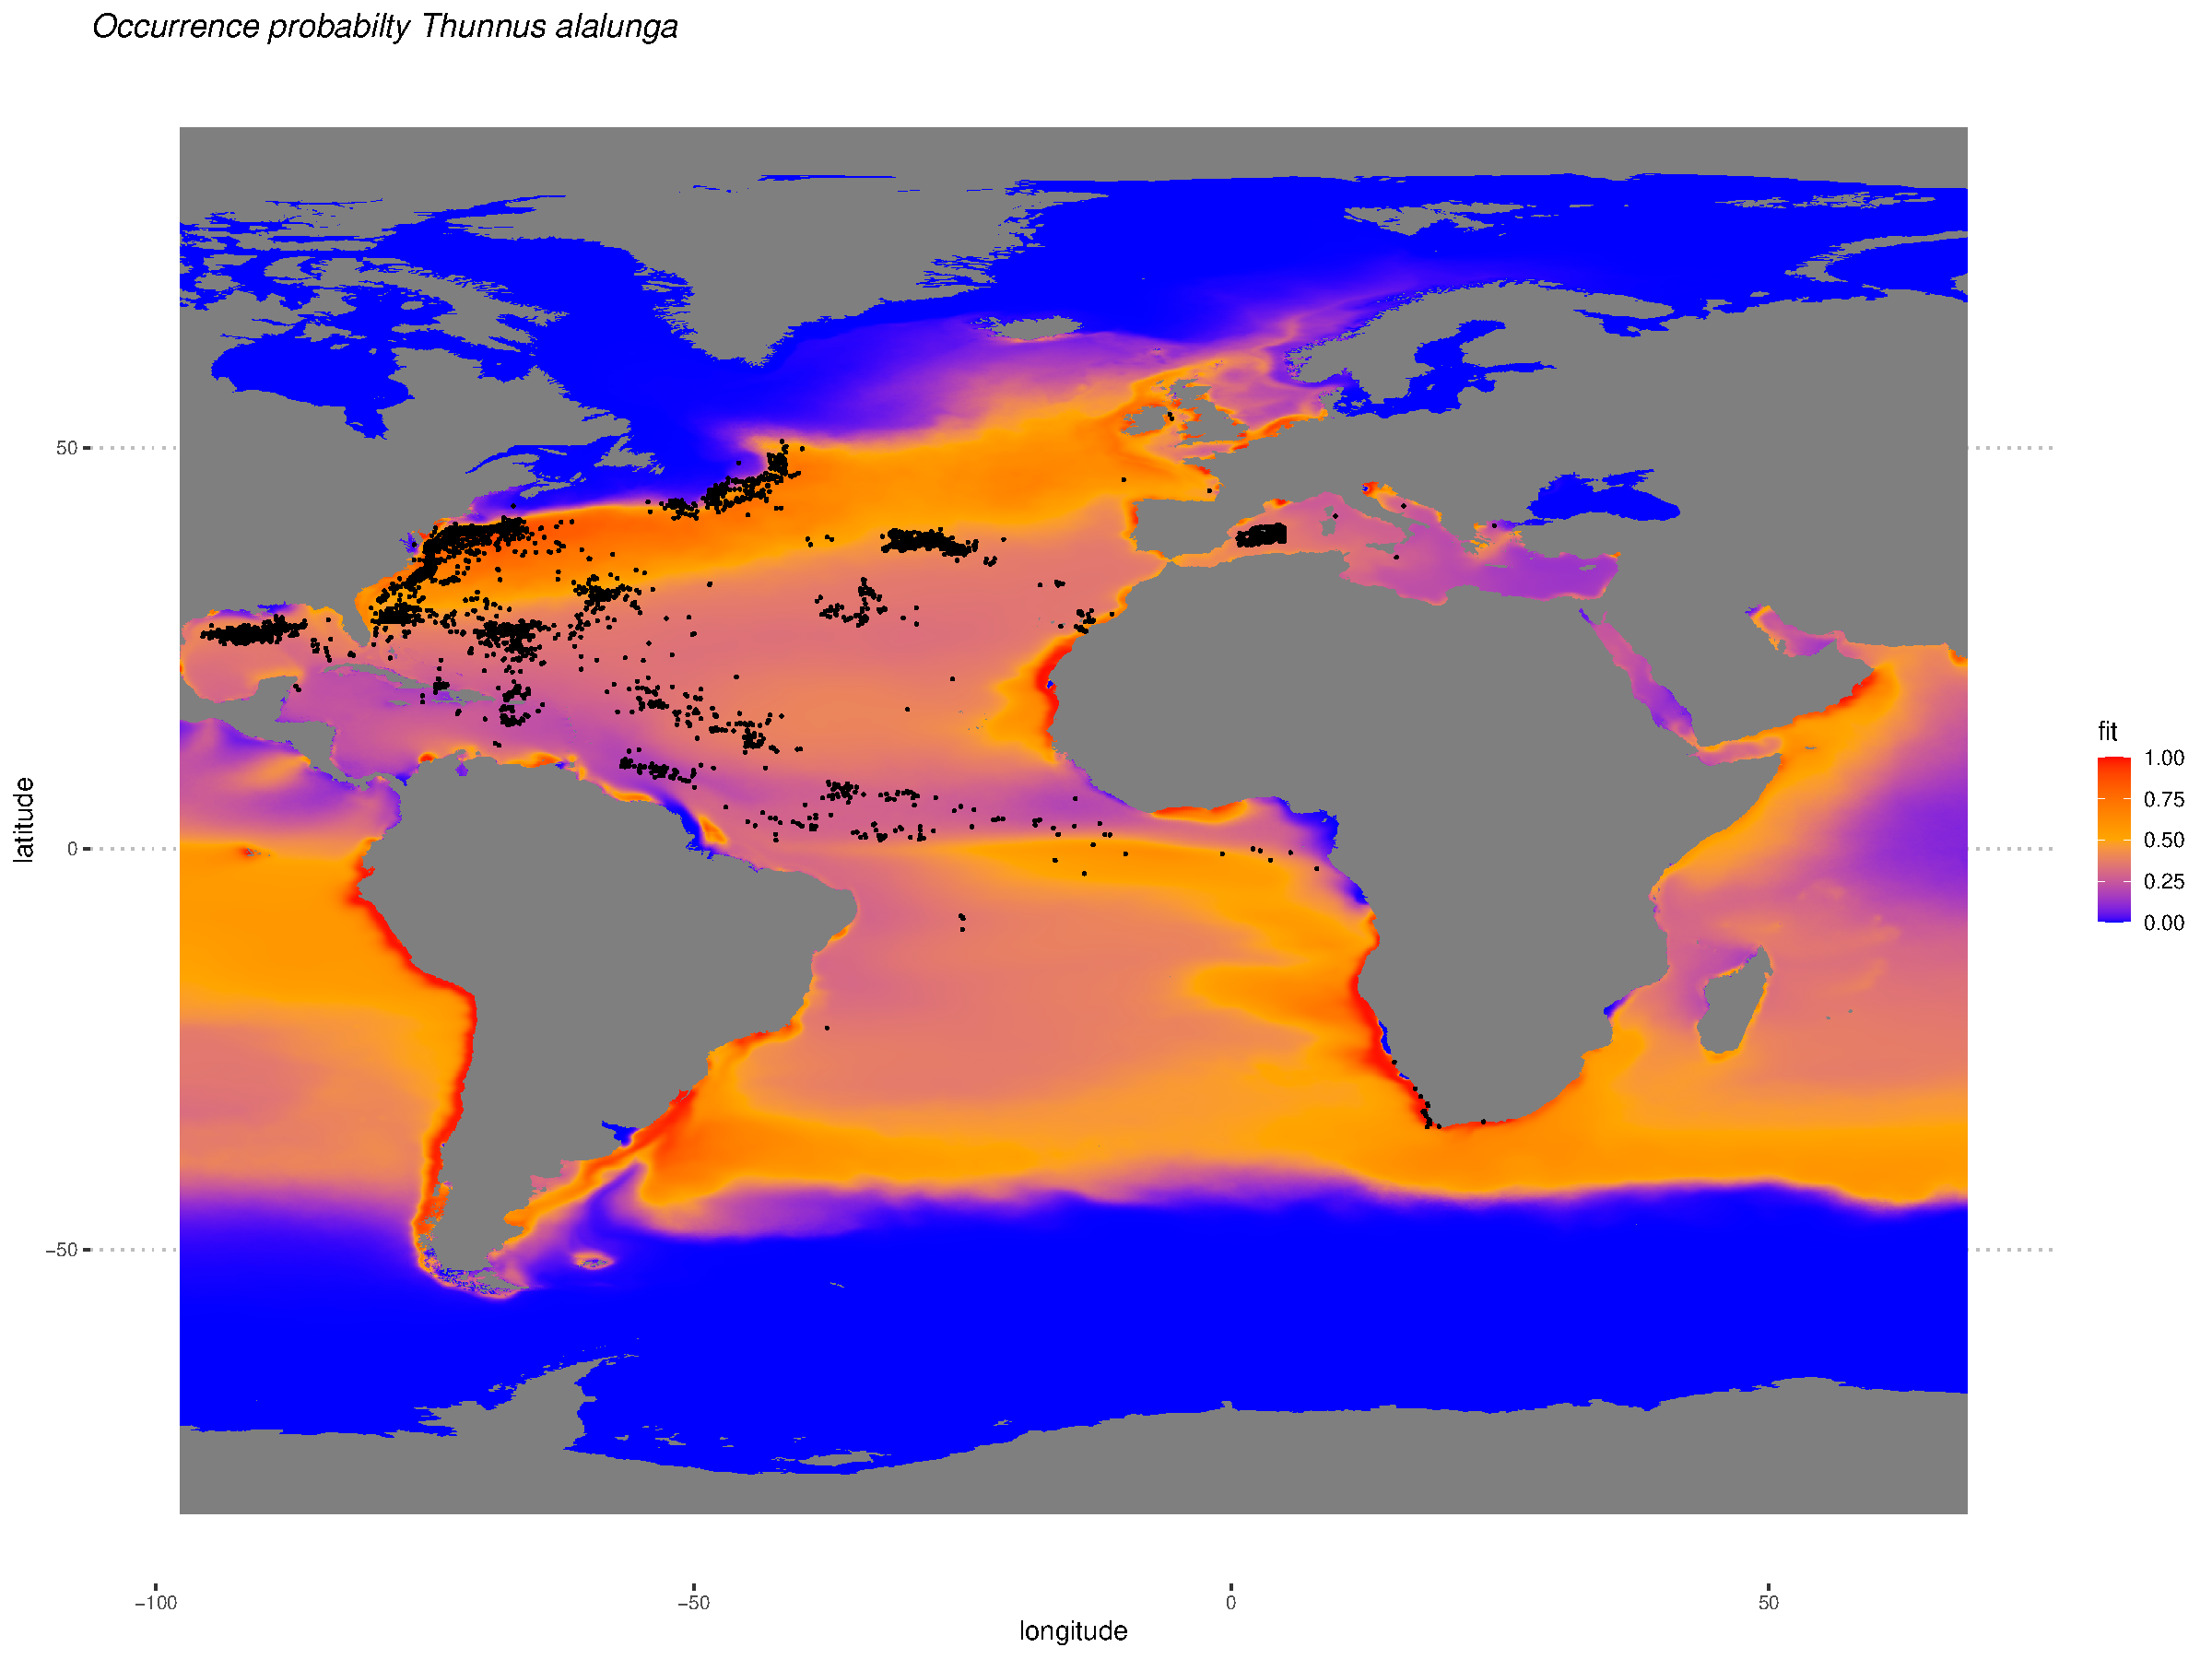
\includegraphics{_main_files/figure-latex/unnamed-chunk-92-1.pdf}

We finally save the projection map.

\begin{Shaded}
\begin{Highlighting}[]
\FunctionTok{ggsave}\NormalTok{(}\AttributeTok{filename=} \StringTok{"Thunnus\_alalunga\_proj\_map.tif"}\NormalTok{, }
        \AttributeTok{plot=}\NormalTok{proj\_map, }
        \AttributeTok{device=}\StringTok{"tiff"}\NormalTok{,}
        \AttributeTok{path=}\NormalTok{here}\SpecialCharTok{::}\FunctionTok{here}\NormalTok{ (}\StringTok{"plots"}\NormalTok{, }\StringTok{"projections"}\NormalTok{), }
        \AttributeTok{height=}\DecValTok{22}\NormalTok{, }\AttributeTok{width=}\DecValTok{30}\NormalTok{,}
        \AttributeTok{units=}\StringTok{"cm"}\NormalTok{, }\AttributeTok{dpi=}\DecValTok{300}\NormalTok{)}
\end{Highlighting}
\end{Shaded}


  \bibliography{references.bib}

\end{document}
